%
% Unless otherwise indicated, the copyright in this material is 
% owned by Joerg Evermann. This material is licensed to you under the 
% Creative Commons by-attribution non-commercial license (CC BY-NC 4.0)}
%
\documentclass{book}

\usepackage[x11names]{xcolor}
\usepackage[most]{tcolorbox}
\usepackage{physics}
\usepackage{wrapfig}
\usepackage{pgf}
\usepackage[english]{babel}
\usepackage[latin1]{inputenc}
\usepackage{times}
\usepackage[T1]{fontenc}
\usepackage{fancyvrb}
\usepackage{multicol}
\usepackage{multirow}
\usepackage{tabularx}
\usepackage{amsmath}
\usepackage{amssymb}
\usepackage{bbm}
\usepackage{alltt}
\usepackage{placeins}
\usepackage{enumitem}
\usepackage{subcaption}
\usepackage{gensymb}
\usepackage{titlepic}
\usepackage{parskip}
\usepackage{imakeidx}
\makeindex[intoc]
\usepackage{hyperref}
\hypersetup{
    colorlinks=true,
    linkcolor=blue,
    filecolor=magenta,      
    urlcolor=blue,
}
\usepackage{subcaption}
%\usepackage{subfigure}
\usepackage{placeins}
\usepackage{minted}
%\usepackage{graphicx}
\newminted{cypher}{autogobble,label=cypher,numbers=left,stepnumber=2,bgcolor=Gray0!25!white,breakbytoken,samepage=true,frame=single}
\newminted{R}{autogobble,label=R,numbers=left,stepnumber=2,bgcolor=Gray0!25!white,breakbytoken,samepage=true,frame=single}
\newminted{xml}{autogobble,label=XML,numbers=left,stepnumber=2,bgcolor=Gray0!25!white,breakbytoken,samepage=true,frame=single}
\newminted{bash}{autogobble,label=bash,numbers=left,stepnumber=2,bgcolor=Gray0!25!white,breakbytoken,samepage=true,frame=single}
\newminted{html}{autogobble,label=HTML,numbers=left,stepnumber=2,bgcolor=Gray0!25!white,breakbytoken,samepage=true,frame=single}
\newminted{js}{autogobble,label=JavaScript,numbers=left,stepnumber=2,bgcolor=Gray0!25!white,breakbytoken,samepage=true,frame=single}
\newminted{sql}{autogobble,label=SQL,numbers=left,stepnumber=2,bgcolor=Gray0!25!white,breakbytoken,samepage=true,frame=single}
\newminted{text}{autogobble,label=Text,numbers=left,stepnumber=2,bgcolor=Gray0!25!white,breakbytoken,samepage=true,frame=single}
\newminted{json}{autogobble,label=JSON,numbers=left,stepnumber=2,bgcolor=Gray0!25!white,breakbytoken,samepage=true,frame=single,escapeinside=||}
\newminted{python}{autogobble,label=Python,numbers=left,stepnumber=2,bgcolor=Gray0!25!white,breakbytoken,python3,samepage=true,frame=single}
\AtBeginEnvironment{minted}{%
  \renewcommand{\fcolorbox}[4][]{#4} \footnotesize}
\AtEndEnvironment{minted}{%
  \normalsize}

\definecolor{code}{gray}{0.95}
\definecolor{alert}{RGB}{238,224,229} % LavenderBlush2 

\newtcolorbox{exercisebox}{enhanced,colback=Gray0!25!white,colframe=Gray0!60!black,title={Hands-On Exercise},fonttitle=\large,leftrule=10mm,overlay={\node[anchor=north west,outer sep=1pt] at (frame.west) {
\includegraphics[width=8mm]{../hand2.png}};}}

\newtcolorbox{resourcebox}{enhanced,colback=LightSteelBlue1!25!white,colframe=LightSteelBlue1!60!black,title={Resources},fonttitle=\large,leftrule=10mm,overlay={\node[anchor=north west,outer sep=0.5pt] at (frame.west) {
\includegraphics[width=8mm]{../book.png}};}}

\newtcolorbox{alertbox}{enhanced,colback=OrangeRed1!25!white,colframe=OrangeRed1!60!black,title=Important,fonttitle=\large,leftrule=10mm,overlay={\node[anchor=north west,outer sep=0.5pt] at (frame.west) {
\includegraphics[width=8mm]{../attention2.png}};}}

\newtcolorbox{infobox}{enhanced,colback=DarkSeaGreen1!25!white,colframe=DarkSeaGreen1!60!black,title=Tip,fonttitle=\large,leftrule=10mm,overlay={\node[anchor=north west,outer sep=0.5pt] at (frame.west) {
\includegraphics[width=8mm]{../tip1a.png}};}}

\newtcolorbox{pseudocodebox}{enhanced,colback=code,colframe=code!50!black}

\renewcommand\floatpagefraction{.95}
\renewcommand\topfraction{.95}
\renewcommand\bottomfraction{.95}
\renewcommand\textfraction{.05}   

\newcommand{\argmax}{\operatorname*{argmax}}
\newcommand{\argmin}{\operatorname*{argmin}}
\newcommand{\Ident}{\operatorname{I}}

\author{Joerg Evermann}
\date{}


\title{Business Analytics}
\author{Joerg Evermann\\
Memorial University of Newfoundland}
\titlepic{\includegraphics[width=\textwidth]{cover1a.png}}

\begin{document}

\frontmatter 

\maketitle

\vfill
\begin{center}
\includegraphics[height=.5in]{by-nc.png}

Unless otherwise indicated, the copyright in this material is owned by Joerg Evermann. This material is licensed to you under the \href{https://creativecommons.org/licenses/by-nc/4.0/}{Creative Commons by-attribution non-commercial license (CC BY-NC 4.0)}
\end{center}

\tableofcontents
\listoffigures
\listoftables

\chapter{Preface}
%
% Unless otherwise indicated, the copyright in this material is 
% owned by Joerg Evermann. This material is licensed to you under the 
% Creative Commons by-attribution non-commercial license (CC BY-NC 4.0)}
%
\section*{Why this book?}

This book is originally intended as material for the BUSI 4720 undergraduate course on Business Analytics. This course is a core, required course for the Bachelor of Commerce program at Memorial University of Newfoundland, Canada. As students receive only a single course in business analytics, and this course is in the fourth and final year of the program, the material coverage is intentionally broad, and covers aspects that may be outside some narrower conceptions of analytics. Additionally, students taking the course generally have little to no exposure to computer applications or statistical software, necessitating a rather comprehensive approach that not only introduces computer and programming basics, such as data and data types that students may encounter in business analytics, but also covers introduction to R and Python as well as a brief coverage of relational and graph databases, that are typically not considered part of business analytics. On the other hand, this course also contains advanced topics, such as interpretable machine learning, analytics at industrial scale, reinforcement and MLOps, that are not usually found in a business analytics course. However, these topics are gaining importance and it is essential that students have at least some exposure to them. In summary, the book was written because no other single book offers the necessary broad perspective. 

The book is written from an applied perspective. I believe that students, even business students, should not only be able to talk about analytics, but must also be able to do analytics. This means that, together with the concepts, every chapter also contains R or Python code showing how the concepts can be applied. Looking at this from another perspective, I believe students must not rely solely on software tools and statistical libraries, but it is crucial that they understand, at least in principle and at an intuitive level, how these tools work. This is necessary to allow an informed use of tools, to be able to select the appropriate tool for a given situation, and to be aware of the shortcomings, drawbacks, boundary conditions, and other limitations of tools. In short, formulas in this book are to explain what happens ''behind the scenes'' of the code, and code is in this book to show how formulas can be applied; both are necessary.

\section*{Why these tools?}

The focus on R and Python, over commercially available tools, is due to multiple reasons. First, the use of open-source software makes the material more easily accessible to students, independent of the availability of campus-wide licenses, or the use of limited ''evaluation'' licenses for some commercial tools. A second reason is the cross-platform nature of these software tools. Computing hardware in practice, and in the classroom, is a heterogeneous mix of different chip sets (Intel, Apple/ARM) and different operating systems (Windows, MacOS, Linux, etc.) so that is essential to work with software tools that are available and interoperable across these hardware and operating system platforms. A third reason is that R and Python are widely used in production environments. They tend to be more flexible than commercial offerings, and are also at the forefront of new developments in the area of business analytics. New methods and techniques are typically implemented directly by their inventor in open-source libraries and packages for R or Python, before they mature and are included in commercial offerings. The focus on command line tools is to avoid the complexities of graphical user interfaces that tend to change more rapidly than application programming interfaces (APIs), it is focus on the essentials and not be distracted by graphical environments. Scripting with command line tools generally also leads to better replicability of analyses and easier integration into production environments. For example, while it is all well and good to explore customer purchasing predictions on a small data set using the desktop edition of SPSS (a commercial, graphical, statistics software application), implementing real-time dynamic pricing in the global web-based ordering system will require the model to be implemented and integrated with very different tools.

\section*{Instructors: How to use this book?}

For instructors, the book is written for a 24 class semester of 75 minutes each (the chapter on visualization should be covered in two classes), with two classes dedicated to mid-term exams. If time is short, some of the later, more advanced chapters could be omitted, for example, the two chapters on reinforcement learning, and/or the chapter on MLOps. A slide set for 22 classes is available, as is a question bank of multiple-choice questions for each chapter, e.g. for quizzes. Each chapter also contains a set of short hands-on exercises that can be used during class to keep students engaged or can form the basis for a computer lab setting. Also available is a set of example exam questions. Given the extensive set of online materials on programming in general, and data science and data analytics in particular, ranging from the traditional \href{Stack Overflow}{https://stackoverflow.com/} site, to Google and YouTube, to the most recent ChatGPT or other LLMs, it is easy for students to complete any technical homework assignment or course project using such tools. Instructors should therefore focus on data and results interpretation and use new or unpublished data sets, if they wish to set such assessment or evaluation exercises at all. Consequently, the example exam questions are long-answer questions that focus on conceptual understanding of the material, and less on technical programming skills.

\section*{Students: How to study?}

For students, accompanying this book is a virtual machine with all required software installed and data sets provided. I recommend that students at least run the provided example code to get some ''hands-on'' with the tools. The best way to learn and understand is to experiment and modify the examples. See what happens when parameters or functions are changed. Ask yourself: Does the result match my expectation? Why or why not? Another way to work with the examples is to make sure you recognize the code elements in the formulas and vice versa. If the formula contains an $X$, where is this specified in the code or where does it appear in the output? Ensure that you can recognize and make the connection between the conceptual or mathematical level and the implementation in software.

Each chapter contains hands-on exercises. These are relatively simple exercises that build directly on the code presented in a section and require only minor changes or adaptations. These exercises invite experimentation with the code and trying different options. They are highly recommended to further your understanding.

Every chapter also contains a number of review questions. These are there to help check your own understanding. At least read and think about the questions, even if you do not write out any answers. 

Many chapters contain pointers to textbooks that formed the basis for the material in this book, and all contain links to online references. These are valuable in that they provide additional, deeper information. And because those resources are written by different authors, they may be easier to understand; at the very least they can provide a different and complementary perspective on the material in this book. Many textbooks that have been used to inform this book are popular or classic textbooks in their own right. Many could form the basis of a somewhat more narrowly conceived course on business analytics. In short, they make for excellent complementary reading and are highly recommended. The vast majority of them are also freely available on the internet.

Additionally, a wealth of information is available in various formats on the internet. This begins with Wikipedia pages, which provide a good introduction to many topics, and material from Wikimedia Commons has been used extensively in this book. Since all the tools used in this book are open-source tools, their web sites provide not only the code, but more importantly, also provide documentation in the form of tutorials, introductions, and detailed programming descriptions. These are all excellent resources. Many researchers and teachers in the area of machine learning have made their materials freely available, for example in their blogs or in YouTube videos and entire YouTube channels. Many of these researchers are active at the forefront of machine learning and are excellent teachers. These resources are valuable resources and provide more depth than offered in this book. At the same time, the current popularity of the topic has also led to some questionable material on the internet, and caution should be exercised when searching for material. Begin your internet search with a trusted source, for example Wikipedia, a well-known researcher, or material from a university instructor active in the field. 

\section*{What about ChatGPT?}

Absolutely consider using your favourite large language model (LLM) for studying this material. For example, ChatGPT is quite good at explaining things. Ask it to explain a code fragment that you copy and paste into it. Ask it to translate R code to Python code or vice versa. Ask it to simplify code for you. Ask it to check code for mistakes. Other ways to engage your favourite LLM are to ask it to quiz you on the material; copy and paste the material into it and then ask it to generate questions and wait for your answer, then to evaluate and correct your answers. Yet another use of an LLM is to a ask it to evaluate and correct your answers to the review questions, provide both the question and your answer to the LLM.
 
These are valuable ways in which you can further your understanding, but keep in mind that LLMs are simply statistical models that predict the most likely next word in the output. As such, they cannot truly reason, they have no intelligence (at least in terms of how we conceive human intelligence) and they make mistakes without being aware of them. So, be careful when you engage them. However, the beauty of using an LLM with computer code is that you can run the code and verify that it does what you expect it to do. 

\chapter{About the Author}
%
% Unless otherwise indicated, the copyright in this material is 
% owned by Joerg Evermann. This material is licensed to you under the 
% Creative Commons by-attribution non-commercial license (CC BY-NC 4.0)}
%

Dr. Joerg Evermann is an associate professor at the Faculty of Business Administration at Memorial University of Newfoundland. He received his PhD in Information Systems in 2003 from the University of British Columbia. Prior to joining Memorial University in 2007, Dr. Evermann was a lecturer in Information Systems with the School of Information Management at the University of Wellington, New Zealand. 

Dr. Evermann's interests are in business process management, statistical methods, and information integration. Dr. Evermann has published his research in more than 80 peer-reviewed publications. His work has appeared in high-quality journals, such as European Journal of Marketing, Decision Support Systems, IEEE Transactions on Software Engineering, IEEE Transactions on Knowledge and Data Engineering, IEEE Transactions on Services Computing, Journal of Business Research, Organizational Research Methods, Structural Equation Modeling, Journal of the AIS, Information systems, and Information Systems Journal. Dr. Evermann has presented his work at international conferences, such as ICIS, AMCIS, CAiSE, ER, among others. He is an associate editor for the Communications of the AIS (CAIS) and the Business Information Systems Engineering (BISE) journals and serves regularly on the program committee of the BPM, ICPM, CBI and AI4BPM conferences and workshops.



\mainmatter

\graphicspath{{class01/}}
\chapter{Introduction}
%
% Unless otherwise indicated, the copyright in this material is 
% owned by Joerg Evermann. This material is licensed to you under the 
% Creative Commons by-attribution non-commercial license (CC BY-NC 4.0)}
%


\section*{Learning Goals}

After reading this chapter, you should be able to:

\begin{itemize}
   \item Differentiate between methods, techniques, and tools.
   \item Describe different types of analytics and their respective goals.
   \item Describe the difference between supervised and unsupervised machine learning.
   \item Describe the different aims of statistics and analytics despite the fact that they often use the same mathematical models.
   \item List some popular software tools for business analytics, and be able to describe why they are widely used and what they are used for.
   \item Use a Linux system using the Terminal window and command line for basic file and folder management.
\end{itemize}

\section{Introduction}

This section describes some of the terminology around the rapidly expanding field of data analytics, business analytics, data science, statistics, machine learning and AI (artificial intelligence). 

\emph{Data analytics} (or simply 'analytics') refers to the broad collection of methods, techniques, and tools to allow humans to make sense of information for purposes of understanding and decision making. Business analytics is the application of data analytics to operational, tactical, or strategic management in businesses and other organizations. Examples are the use of visualization of human resource performance data, trend analysis of outbound logistics costs, prediction of customer demand, fraud analysis of financial transactions, and others.

Data analytics as a broad field is closely related to a range of other fields, such as data management (how best to collect, store, access, and use data in a variety of format), visualization (how best to present data in an easy-to-understand format to generate insights or persuade stakeholders), machine learning (how to train computers to classify data and to make predictions), or text analysis (how to extract meaningful information from natural-language text information). Some argue that these fields are within analytics, but others view them as separate but strongly interrelated. For example, text analysis and machine learning overlap when training computers to predict customer behaviour based on social media post data. Text analysis can provide certain features that characterize or summarize a text, and may be used as input for machine learning. Machine learning models can exploit text-specific features, such as the sentence structure, in making predictions. Training machine learning systems also requires a very large amount of data, so advanced data management techniques are required in order to store and provide this data in an efficient way. 

\emph{Artificial Intelligence (AI)} is a field with a long and varied history, going back to the 1960s. Originally, AI was used for symbolic computations, where researchers attempted to explicitly describe and model human reasoning processes in a computer. In the late 1990s and early 2000s, AI has morphed to focus on statistical models and has most recently become dominated by artificial neural networks (ANN) and deep neural networks (DNN), a field called deep learning. Artificial neural networks, while inspired by the human brain, are essentially statistical models for classification and regression, akin to the simple linear or logistic regression. But whereas the simplest linear regression model may describe a small dataset of hundreds to thousands of observations using just two parameters (the slope and intercept), ANN and DNN are non-linear and highly complex with millions or even billions of parameters and are often trained on billions of observations. However, the main ideas are the same in that the model is trained on or fitted to a data set. 

More recently, since about 2020, \emph{generative AI}, that is, AI models and systems that are used to generate text, images, audio or video in response to user input has become synonymous with AI. The rise in popularity of systems such as ChatGPT, Dall-E, and many others, has led to many people equating AI with generative AI.

While \emph{machine learning} may sometimes be viewed synonymously with ANN or DNN, the field of machine learning is broader than just neural network models and concerns the development of methods to make predictions for new observations. Traditional statistical techniques for regression and classification, such as decision trees or support vector machines, are considered part of machine learning, and therefore also part of data analytics. However, these statistical models sometimes take a back seat role compared to ANNs because of the power and flexibility of the latter. 

Machine learning and AI are also sometimes viewed synonymously. However, as noted above, there are subfields of AI that are not concerned with machine learning and prediction. First, research into symbolic reasoning is still ongoing. Second, methods such as reinforcement learning, which focuses not on making predictions, but on prescribing optimal courses of action, are considered part of machine learning and AI.

\emph{Big Data} was an important topic in the early 2000s and 2010s but is now often considered a sub-field of data analytics or data science. The motivation for Big Data was the recognition that the volume of data produced and available for analysis has been growing exponentially since the 1990s. This has spurred the development of advanced data management methods, techniques, and tools, such as distributed file systems and databases. The velocity of data, that is, its rate of production, has also increased greatly since the 1990s. Processing the data often has to occur in real-time, leading to development of techniques and tools that can analyze data ''on-the-fly'' (''stream processing'').

Finally, the term \emph{data science} is often used in a less applied and more scientific or research and developmental way than the term data analytics, to characterize the development, rather than application, of methods, techniques, and tools.

\section{Methods, Techniques, and Tools}

In the context of data science and data analytics, methods, techniques, and tools play distinct roles in the process of extracting insights from data. \emph{Methods} encompass overarching approaches and strategies, providing a systematic framework for tasks such as data exploration, modeling, and analysis. These high-level methodologies guide data scientists in formulating a structured plan for addressing specific challenges or achieving analytical goals.

\emph{Techniques} in data science are the specific procedures and practices employed within the broader methodological framework. These practical and detailed approaches are applied to handle particular aspects of the data analysis process. For instance, in exploratory data analysis, techniques like histograms or scatter plots are used to visually inspect data distributions or relationships between variables and in classification, a naive Bayes classifier is considered a specific technique.

\emph{Tools} in data science refer to the instruments and software applications that facilitate the practical application of methods and techniques. These can range from programming languages like Python and R, statistical packages such as Pandas and SciPy, to visualization tools like Shiny or Matplotlib. The selection of appropriate tools is crucial for efficiently executing data science tasks and optimizing the workflow.

\section{Types of Analytics}

There are different ''types'' of analytics that have different aims. 

\paragraph*{Descriptive Analytics} describes ''what is''. It typically provides summaries of the data, makes comparisons between different types of entities or measurements, may identify historical trends, or provide rankings of observations or measurements. An example is the identification and comparison of current and historical costs to manufacture different widgets in different plants. Another example are the identification of the top-grossing sales people in the organization for specific product types, or calculating the the mean cycle time of the order-to-cash business process for different time periods. Descriptive analytics is therefore important in a business context and organizations expend a great deal of money, time, and effort on technologies such as report generating tools to support this type of analytics. 

\paragraph*{Predictive Analytics} describes ''what may be'' in the future. It typically builds a \emph{model} based on past data to predict future cases/events/outcomes. As a simple example, consider a linear regression model that predicts the overall spending of a customer from their income. One can build a linear model with parameters for the intercept and slope and then train the model on customers whose spending and income are known. Training means to determine the two parameters of the model so that they model best fits the data. Given a trained model, one can then predict the overall spending of a new customer given their income. Of course, the models can be much more complex than a simple linear regression, and often have tens, hundreds, thousands, or even millions of parameters, but the principle of model-based predictive analytics remains the same.

\paragraph*{Prescriptive Analytics} describes ''what should be done''. Similar to predictive analytics, a model is usually built from  past data. However, the model must now also consider which actions can be taken (and were taken for the past training data). In reinforcement learning, a popular prescriptive analytics technique, one assumes that an \emph{agent} can observe the state of an \emph{environment}, can take \emph{actions} based on the observed state, and receives a (positive or negative) reward from the environment after taking an action. Actions may change the state of the environment. The agent must learn to identify those actions in each state that give it the maximum rewards. The optimal actions are called a \emph{policy} and can then be used to prescribe which action to take in which state.

\paragraph*{Visual Analytics} describes the use of graphs (plots, diagrams) to visualize information for exploring data and gaining insight. Visual analytics makes use of the human ability to visually identify trends, make comparisons, etc. In effect, this type of analytics supports humans in their tasks. It employs no mathematical or statistical models. However, humans may identify features of the data such as trends, comparisons, etc. with visual analytics that may then be tested with statistical models or form the basis on which to build predictive or prescriptive analytics models. 

\section{Machine Learning}

In the context of analytics, machine learning (sometimes simply called ''learning'') can be divided into supervised and unsupervised learning. \emph{Supervised learning} is typically based on a parameterized statistical or mathematical model. For example, a simple linear regression is based on two parameters, the slope and intercept. Models are trained (that is, parameters are estimated) by adjusting the model parameters so that the model's output (e.g. the predicts value ''$\hat{y}$ in a linear regression) for each given input (e.g. the ''x'' value in a linear regression) matches the actually observed outcome (the ''y'' value in a linear regression). Supervised learning assumes that a correct/observed outcome is available for all inputs. Linear regression is a very simple supervised learning approach with a simple statistical model; on the other extreme there are generative pre-trained transformer (GPT) models that predict words for generating text, and which contain billions of parameters and non-linear relationships among them.

\emph{Unsupervised learning} on the other hand does not require outcome values and only requires ''input'' (''x'') values. Typical unsupervised learning tasks are clustering and dimensionality reduction. For example, one may form clusters of widgets at the end of a production line based on how similar the widgets are on different characteristics that were measured by sensors. These clusters could then, for example, be interpreted as quality grades. Similarly, customers may be clustered based on their past transactions or purchases. Different marketing strategies may then be applied to each cluster. The aim of dimensionality reduction is to be able to describe a data set with many variables by using only a few variables. Imagine that having hundreds of different characteristics of widgets. One might then wish to simplify and identify fewer, perhaps as few as two or three, combinations of the original characteristics that provide the same information about the widgets.

\section{Analytics is not Statistics}

Analytics and statistics use the same kinds of mathematical models. However, ''traditional'' \emph{statistics} focuses on sample and population characteristics, such asmeans, slopes, intercepts, and others, of a sample or a population that are represented as parameters of a mathematical model. Statistics aims to identify and explain the data generating mechanism, i.e. the ''real world'' or population. In particular, \emph{inferential statistics} is used to generalize from a sample to a population. Importantly, statistics is typically not concerned with individual cases or individual observations.

In contrast, data analytics, especially predictive analytics, focuses on predicting the outcome of an individual case or observation. Analytics is pragmatic, in that models are considered useful tools and do not need to faithfully describe the ''real world'' or the data generating mechanism, as long as they make good predictions or are otherwise useful for their purpose. Consequently, there is no inference from sample to population, because the model does not claim to describe a population. The quality of a model is determined not by its fit with the observed data, but by its precision or accuracy when predicting specific observations. 

\section{Tools used in this Course}

The software used in this course is open-source and free software. Open-source software (OSS)\index{Open-source software}\index{OSS|see{Open-source software}} embodies a collaborative approach to software development, allowing users to access, modify, and distribute the source code freely\footnote{\url{https://en.wikipedia.org/wiki/Open-source_software}}. This approach promotes transparency, enabling users to inspect the code, modify, adapt, fix and extend it, and contribute to its improvement. 

Free software\index{Free software}, as defined by the Free Software Foundation (FSF), goes beyond accessibility, emphasizing users' fundamental freedoms to run, study, modify, and share the software\footnote{\url{https://en.wikipedia.org/wiki/Free_software}}. Contrary to the common misconception, "free" in this context pertains to freedom, not necessarily zero cost. The ethical philosophy behind free software underscores the importance of user control over technology. 

The term FOSS\index{Free and open-source software}\index{FOSS|see{Free and open-source software}}, or Free and Open-Source Software\footnote{\url{https://en.wikipedia.org/wiki/Free_and_open-source_software}}, serves as an inclusive label encompassing both the principles of free software and the collaborative nature of open-source software. FOSS encourages a shared approach to software development, emphasizing not only the technical benefits of open code but also the ethical imperative of user freedom and community-driven innovation.

Free and Open-Source Software (FOSS) \emph{licenses} are legal agreements that govern the use, modification, and distribution of open-source software. These licenses play a crucial role in preserving the core principles of freedom, transparency, and collaboration within the open-source community. Common characteristics of FOSS licenses are:

\paragraph*{Freedom to Use} FOSS licenses grant users the freedom to use the software for any purpose without any restrictions.

\paragraph*{Freedom to Study} Users have the right to access and study the source code of the software. This transparency allows for a deeper understanding of how the software functions.

\paragraph*{Freedom to Modify} FOSS licenses typically allow users to modify the source code according to their needs. This encourages innovation, customization, and adaptation of the software.

\paragraph*{Freedom to Share} Users can distribute both the original and modified versions of the software, fostering a collaborative environment. This freedom to share is fundamental to the open-source philosophy.

\paragraph*{Copyleft Licenses} Some FOSS licenses, such as the GNU General Public License (GPL), include copyleft provisions. Copyleft ensures that any derivative works or modifications are also subject to the same open-source terms. This prevents the software from being incorporated into proprietary projects without maintaining open-source characteristics.

\paragraph*{Permissive Licenses} On the other hand, permissive licenses, like the MIT License and the Apache License, allow for more flexibility. They permit the use of the software in proprietary projects without imposing the requirement to open-source the derived code.

While a lot of free and open-source software used to be developed by individuals, increasingly FOSS is developed by companies whose business model rests either on providing paid support for such tools, or on providing paid hosted versions of the software, or on providing non-free extensions for their FOSS software. In other cases, companies provide software developer time to important projects that benefit themselves.

\begin{table}
\small
\centering

\begin{tabular}{l|l|l} \hline
R & 4.1.2 & \url{www.r-project.org}\\ 
dplyr & 1.1.3 & \url{www.tidyverse.org} \\
tidyr & 1.3.0 & \url{www.tidyverse.org} \\
ggplot2 & 3.4.4 & \url{www.tidyverse.org} \\
Python & 3.8 & \url{www.python.org} \\
numpy & 1.24.4 & \url{numpy.org} \\
pandas & 2.0.3 & \url{pandas.pydata.org} \\
plotly & 5.18.0 & \url{plotly.com} \\ 
tensorflow & 2.13.1 & \url{www.tensorflow.org} \\
Postgres & 16.0-1 & \url{www.postgresql.org} \\
pgAdmin4 & 7.8 & \url{www.pgadmin.org} \\
PyCharm & 2023.2.3 & \url{www.jetbrains.com/pycharm/} \\
Jupyterlab & 4.0.7-1 & \url{//github.com/jupyterlab/jupyterlab-desktop} \\
Neo4J & 5.14.0 & \url{www.neo4j.com} \\ \hline
\end{tabular}
\caption[Software used in this book]{Software used in this course}
\label{tab:software}
\end{table}

\subsection*{The R System}

\begin{wrapfigure}{l}{1in}
\begin{center}
\includegraphics[height=.5in]{R_logo.png}
\end{center}
\end{wrapfigure}
R is is a programming language and free software environment designed for statistical computing and graphics. 

The history of R begins in the early 1990s at the University of Auckland, New Zealand. Ross Ihaka and Robert Gentleman, two statisticians, set out to create a programming language that would make data analysis and visualization more accessible. They released the first version of R in 1995, and it quickly gained traction within the academic community.

Over the years, R evolved and expanded its capabilities, thanks to the collaborative efforts of statisticians, data scientists, and programmers worldwide. The Comprehensive R Archive Network (CRAN) was established to serve as a hub for R packages, fostering a community-driven approach to software development.

The open-source nature of R played a pivotal role in its success. As more people embraced it, R became not just a statistical tool but a versatile platform for data analysis, machine learning, and graphical exploration. Its popularity soared in both academic and industry settings, with businesses recognizing its potential for extracting meaningful insights from data.

R continues to thrive as a dynamic and evolving tool in the world of data science. Its rich ecosystem of packages and active community ensure that it remains at the forefront of statistical computing and analysis. 

One of the key hubs of the R community is the Comprehensive R Archive Network (CRAN), where thousands of R packages are hosted. These packages cover a vast array of topics, from basic statistical functions to cutting-edge machine learning algorithms. The "open-source" ethos is strong here, with contributors from around the globe actively developing and maintaining packages.

Stack Overflow\footnote{\url{https://stackoverflow.com/collectives/r-language}} and other online forums serve as virtual interchanges of ideas where R users exchange knowledge and troubleshoot problems.

The tidyverse\footnote{\url{https://www.tidyverse.org/}} is a comprehensive collection of R packages that share a common philosophy and syntax, designed to streamline and enhance the data analysis workflow. Developed by Hadley Wickham and his collaborators, the tidyverse promotes a principled approach to data manipulation, visualization, and exploration. Key components are:

\paragraph*{ggplot2} A sophisticated and flexible plotting system, ggplot2 enables the creation of intricate and publication-ready visualizations. Its grammar of graphics approach provides a consistent framework for constructing a wide range of plots.

\paragraph*{dplyr} This package serves as a cornerstone for data manipulation, offering a set of succinct and expressive verbs for tasks such as filtering, grouping, summarizing, and joining datasets. Its syntax facilitates a more intuitive and readable coding style.

\paragraph*{tidyr} Complementing dplyr, tidyr focuses on reshaping and tidying data. It provides functions like `gather()` and `spread()` to efficiently restructure datasets, ensuring they adhere to the principles of tidy data.

\paragraph*{readr} A fast and user-friendly package for reading and parsing data from various file formats. readr's emphasis on speed and consistency makes it a reliable choice for importing datasets seamlessly.

The tidyverse's cohesive design and interoperability between packages make it a popular choice for data scientists and analysts seeking an efficient and coherent ecosystem for their R-based projects.

\subsection*{Python}

Python\footnote{\url{www.python.org}}, conceived by Guido van Rossum in the late 1980s and released in 1991, has evolved into a versatile and influential programming language. Known for its readability and clean syntax, Python prioritizes simplicity and ease of use, making it accessible to both beginners and seasoned developers. The Python Software Foundation now oversees its development, ensuring that it remains free, open, and continually improved by a global network of contributors.

\begin{wrapfigure}{l}{1.5in}
\begin{center}
\includegraphics[height=.5in]{python-logo.png}
\end{center}
\end{wrapfigure}

One of Python's key strengths is its versatility. It serves as a general-purpose language, excelling in web development, data analysis, artificial intelligence, scientific computing, and more. Its extensive standard library and a rich ecosystem of third-party packages contribute to its adaptability across diverse domains.

Python's readability, enforced by the use of indentation for block delimiters, facilitates code comprehension and maintenance. This, coupled with a strong emphasis on code readability and maintainability, has contributed to its popularity among developers.

Python's adoption in data science has surged, with libraries such as NumPy, pandas, and scikit-learn forming the backbone of numerous data analytics and machine learning projects.

The language's cross-platform compatibility, supported by its interpreted nature, allows developers to write code once and run it on various operating systems without modification. This, combined with a vast and active community, ensures that Python remains at the forefront of technological advancements.

In the Python ecosystem, packages play a crucial role in extending the language's functionality and addressing specific programming needs. Python packages are collections of modules, scripts, and other resources that facilitate the development of reusable and modular code. Pip (Package Installer for Python) is the default package installer for Python, allowing users to easily install, upgrade, and manage Python packages. It simplifies the process of fetching and installing packages from the Python Package Index (PyPI) and other repositories. PyPI is the official repository for Python packages, hosting a vast collection of open-source Python software.

\paragraph*{NumPy} NumPy, short for Numerical Python, is a fundamental library in the Python ecosystem for numerical computing. Developed to facilitate array operations, mathematical functions, and linear algebra capabilities, NumPy provides a foundation for scientific and data-intensive applications.

Launched in 2005 by Travis Olliphant, NumPy has become a cornerstone in the Python data science stack. Its core feature is the ndarray, a multidimensional array object that enables efficient manipulation of large datasets. NumPy's array-oriented computing paradigm enhances performance and readability, making it a preferred choice for numerical tasks.

\paragraph*{Pandas} Pandas, a Python library introduced in 2008 by Wes McKinney, is an important tool in data manipulation and analysis. Designed to provide high-performance, easy-to-use data structures, Pandas simplifies the handling of structured data and time series.

At its core are two primary data structures: the Series, a one-dimensional labeled array, and the DataFrame, a two-dimensional table with labeled axes. These structures, built on top of NumPy arrays, empower users to perform a range of operations from basic data cleaning to complex analytics, with a concise and expressive syntax.

Pandas can handle missing data gracefully and offers easy to use tools for reshaping, grouping, and aggregating data. Its integration with other Python libraries, coupled with efficient indexing and alignment features, makes it a good choice for data scientists, analysts, and researchers working with heterogeneous and large datasets.

\paragraph*{Tensorflow and Keras} 

\begin{wrapfigure}{r}{1.5in}
\begin{center}
\includegraphics[height=1in]{Tensorflow_logo.png}
\end{center}
\end{wrapfigure}

TensorFlow is an open-source machine learning framework initially developed by the Google Brain team. It provides a comprehensive set of tools and libraries for building and deploying machine learning models. TensorFlow facilitates the creation of artificial neural networks and other machine learning models through a flexible and scalable platform. 

Keras is an open-source high-level neural networks API written in Python. Originally developed as an independent library, it has become an integral part of TensorFlow, serving as its official high-level programming interface. Keras simplifies the process of building, training, and deploying neural networks, making it accessible to developers of different skill levels. While Keras is designed to be user-friendly and concise, TensorFlow provides a more extensive and low-level framework for those requiring greater flexibility in model design and customization. 

\paragraph*{PyCharm} 

\begin{wrapfigure}{r}{1in}
\begin{center}
\includegraphics[height=.5in]{PyCharm_icon.png}
\end{center}
\end{wrapfigure}

PyCharm by JetBrains is an integrated development environment (IDE) for Python developers. PyCharm Community is its free and open-source version. The IDE includes a code editor with syntax highlighting, code completion, and error checking, supporting developers in writing clean and efficient code. PyCharm's code navigation and refactoring tools facilitate easy exploration and improvement of code bases. The built-in debugger and seamless integration with testing frameworks like pytest enhance debugging and testing capabilities. PyCharm also supports version control systems, including Git and Mercurial, promoting collaborative development. PyCharm has a user-friendly interface, continuous updates, and active support.

\paragraph*{Jupyter, JupyterLab, JupyterLab Desktop} 

\begin{wrapfigure}{r}{1in}
\begin{center}
\includegraphics[height=.5in]{Jupyter_logo.svg.png}
\end{center}
\end{wrapfigure}

Jupyter Notebooks are interactive computing environments that allow users to create and share documents containing live code, equations, visualizations, and narrative text. Originally developed for Python, Jupyter Notebooks support multiple programming languages through various kernels. The notebooks are structured as a series of cells, where each cell can contain code, markdown text, or rich media elements. Users can execute code cells interactively, see immediate outputs, and create a seamless blend of code and documentation.

JupyterLab is an extensible web-based interactive computing environment developed by the Jupyter Project. It serves as the next-generation interface for Jupyter Notebooks, offering a more versatile and powerful environment. JupyterLab provides a flexible and modular interface where users can arrange documents, notebooks, terminals, and custom components in a tabbed layout. It supports multiple Jupyter Notebooks simultaneously and allows for drag-and-drop functionality to rearrange and organize the workspace. JupyterLab's extensibility comes from its plugin system, enabling users to add new features and customize the environment to suit their workflows.

JupyterLab Desktop refers to the stand alone application version of JupyterLab that runs on a user's desktop rather than in a web browser. It offers the same rich features as the web-based version but provides a stand alone application that can be launched independently. JupyterLab Desktop enhances user accessibility and convenience, providing a familiar desktop application experience for working with Jupyter Notebooks and other interactive computing tasks.

\subsection*{PostgreSQL}

\begin{wrapfigure}{l}{1in}
\begin{center}
\includegraphics[height=.5in]{postgresql-logo.png}
\end{center}
\end{wrapfigure}

PostgreSQL is an open-source relational database management system (RDBMS) whose history goes back to the mid-1980s when a team led by Michael Stonebraker at the University of California, Berkeley laid the foundation for what would later become PostgreSQL.

PostgreSQL has been characterized by standards compliance, extensibility, and robustness. Over the years, it has evolved into a feature-rich and reliable database system that caters to a wide range of applications. One of PostgreSQL's key strengths lies in its extensibility and support for custom data types, operators, and functions. This flexibility empowers developers to model and store data in ways that suit the specific needs of their applications. Furthermore, PostgreSQL boasts support for advanced indexing techniques, complex queries, and transactional consistency, making it well-suited for high-performance and mission-critical environments.

The commitment to data integrity is a hallmark of PostgreSQL. It provides support for ACID (Atomicity, Consistency, Isolation, Durability) properties, ensuring the reliability of transactions. Additionally, features like point-in-time recovery and built-in replication mechanisms contribute to the system's resilience and availability.

\subsection*{Neo4j}

\begin{wrapfigure}{l}{2in}
\begin{center}
\includegraphics[height=.5in]{neo4jlogo.png}
\end{center}
\end{wrapfigure}

Neo4j is a graph database management system, designed to handle and store data in a graph structure rather than in traditional tables. In Neo4j, data is represented as nodes, edges, and properties. Nodes typically represent entities such as people, businesses, accounts, or any other item you might find in a dataset. Relationships provide the connections between these nodes, akin to how foreign keys work in relational databases, but with a more natural and direct approach to represent how items are related. This structure makes it particularly efficient for querying complex and deeply interconnected data.

One of the key strengths of Neo4j is its powerful query language, Cypher, which allows for expressive and efficient querying and manipulation of the graph data. Cypher is designed to be intuitive and readable, focusing on the clarity of expressing what data to retrieve or how to manipulate the data, rather than how to navigate the structure. This makes it easier to model complex relationships and query them efficiently. Neo4j is a popular choice for applications that require complex data relationships and network analysis, such as social networks, recommendation systems, and fraud detection.

\section{Ubuntu Linux}

\begin{wrapfigure}{l}{1.5in}
\begin{center}
\includegraphics[height=.5in]{Ubuntu-logo.png}
\end{center}
\end{wrapfigure}

Ubuntu Linux, developed and distributed by Canonical Ltd., has emerged as a popular distribution within the Linux ecosystem since its first release in 2004. Through its commitment to ease-of-use and pragmatic approach to hardware compatibility, Ubuntu has played a significant role in popularizing Linux as a viable alternative to proprietary operating systems. The operating system's development is steered by a global community of contributors who collaborate on various aspects, from bug fixes to the introduction of new features.

One distinguishing feature of Ubuntu is its emphasis on regular and predictable release cycles. This approach ensures that users have access to the latest software updates, security patches, and improvements. Ubuntu's Long Term Support (LTS) releases, occurring every two years, provide a support window of 5 years, offering stability and reliability for enterprises and users seeking a more predictable environment.

The desktop edition of Ubuntu employs the GNOME desktop environment, providing an intuitive and user-friendly interface. Ubuntu's package management system, APT, simplifies the installation and removal of software packages. It uses the ''apt'' command line tool or the ''Synaptic'' graphical interface to APT. The extensive and well-maintained software repositories contribute to Ubuntu's versatility, allowing users to access a rich ecosystem of applications without the need for extensive manual configurations. Because Ubuntu is based on Debian, it can use Debian packages and packages in the Debian package format.

\begin{center}
\includegraphics[height=3in]{screenshot1.png}
\end{center}

As a multi-user operating system, Ubuntu provides support for file permissions for each user, user home directories, and user privileges. User home directories are typically located in \texttt{/home/<userName>/} and the \texttt{sudo} (''\underline{s}uper\underline{u}ser do'') command may be used to execute commands as super user (equivalent to the ''root'' user in Linux terminology).
 
\begin{wrapfigure}{r}{1.in}
\begin{center}
\includegraphics[height=.5in]{Virtualbox_logo.png}
\end{center}
\end{wrapfigure}
 
\section{Virtual Machines}
 
Virtualization with virtual machines\index{Virtual machine}\index{Virtualization|see{Virtual machine}} allows users to create an run virtual computers on their own computers, enabling the installation and operation of multiple operating systems simultaneously. The ''real'' system that is running the virtualization software application is called the host system or host operating system, while the virtual computer running inside the virtualization software is called the guest system, or guest operating system. In effect, the virtualization software pretends to be an actual computer to the guest system, and the guest system is a complete operating system, such as Windows or Linux.

VirtualBox is a free and open-source virtualization software application developed by Oracle. VirtualBox is available for host systems with an Intel or AMD processor, running Windows, MacOS, or Linux operating systems. VirtualBox supports a wide range of guest operating systems, including various versions of Windows, Linux distributions, MacOS, BSD, and others. VirtualBox provides "Guest Additions," which are additional software packages that can be installed on the guest operating system. These additions enhance the performance and integration between the host and guest systems, providing features like seamless mouse integration, shared folders, and improved graphics support. 

VMWare Fusion is a proprietary virtualization software owned by Broadcom. VMWare Fusion is available for Apple Mac computers running either Intel processors (before circa 2021) or the later Apple M1, M2 or M3 processors (after circa 2021). Similar to VirtualBox, it allows users to create and run virtual machines on their computer and provides a way to share folders from the host system to the guest system, and to copy and paste from host to guest and vice versa. \\
 
\begin{alertbox}
Virtual machine files for use with VirtualBox and VMWare Fusion may be provided by your instructor that contains an Ubuntu system with all required software installed. If you wish to use this, you must install VirtualBox or VMWare Fusion on your computer, then download the corresponding virtual machine file and import it into the virtualization software application.  \\

The username is \textbf{busi4720} and the password is \textbf{busi4720}. Whenever a password is required, you should enter \textbf{busi4720}.
\end{alertbox}
  
\begin{alertbox}
If you do NOT wish to use the VirtualBox Appliance, you should download and install all software to your computer from the sources indicated in Table~\ref{tab:software} in (at least) the versions indicated in the table.
\end{alertbox}
 
\section{The Ubuntu Command Line (also for Mac Users)}

This tutorial provides a very brief introduction to the Ubuntu command line (''terminal''). The command line, also called a ''shell'' is by default the ''bash'' shell (Bourne-again shell; a pun on the earlier Bourne shell)\index{Bash|see{Bourne-again shell}}\index{Bourne-again shell}. In Ubuntu, you can open the Terminal application using the key combination \fcolorbox{black}{lightgray}{Ctrl-Alt-T}, or by selecting the Terminal application icon from the side bar or the application list. You can also open a Terminal from the file browser. \\

\noindent \emph{Note:} The default shell in the MacOS terminal is the ''zsh'' and behaves slightly differently from the bash shell. You can work with a ''bash'' shell by typing the \texttt{bash} command in a MacOS terminal.

\begin{resourcebox}
The following are further beginner-level tutorials on using the command line on Ubuntu (or any other Linux distribution):
\begin{itemize}
\item \href{https://ubuntu.com/tutorials/command-line-for-beginners}{Ubuntu command line for beginners}
\item \href{https://www.digitalocean.com/community/tutorials/a-linux-command-line-primer}{Linux command line primer}
\item \href{https://www.digitalocean.com/community/tutorial-series/getting-started-with-linux}{Getting started with Linux}
\end{itemize}
\end{resourcebox}


Bash will show you a \emph{command prompt} that indicates your username (''busi4720''), the name of the computer (''busi4720vm'') and your current working directory (''$\sim$'') followed by the dollar sign ''\$''.

\noindent\underline{P}rint the \underline{w}orking \underline{d}irectory by typing the \texttt{pwd} command and then pressing the \fcolorbox{black}{lightgray}{Return} or \fcolorbox{black}{lightgray}{Enter} key:
\begin{bashcode}
busi4720@busi4720vm:~$ pwd
/home/busi4720
\end{bashcode}

\noindent\underline{M}a\underline{k}e a folder/\underline{dir}ectory with the \texttt{mkdir} command (in your current working directory):
\begin{bashcode}
busi4720@busi4720vm:~$ mkdir someFolder
\end{bashcode}
\noindent\underline{C}hange the working \underline{d}irectory to the folder you have just created with the \texttt{cd} command. Note how the Bash command prompt indicates your new working directory. 


\begin{bashcode}
busi4720@busi4720vm:~$ cd someFolder
busi4720@busi4720vm:~/someFolder$ cd ..
busi4720@busi4720vm:~$ cd ~
\end{bashcode}

\noindent The following special characters can be used when specifying folders/directories and paths:\\

\begin{tabular}{l|l} \hline
\texttt{$\sim$} & User home directory \\
\texttt{.} & Current directory \\
\texttt{..} & Upwards in the directory tree \\
\texttt{/} & Root of directory tree \\ \hline
\end{tabular} \\

\noindent Here are some tips that make working with the shell a lot easier:

\begin{itemize}
  \item Autocompletion of file names is available with the ''\fcolorbox{black}{lightgray}{Tab}'' key. When multiple file names exist that match what you have entered so far, you can enter further characters of a file name to disambiguate and press the \fcolorbox{black}{lightgray}{Tab} key again for further autocompletion. 
  \item You can recall earlier commands with the ''\fcolorbox{black}{lightgray}{Up Arrow}'' key. By default, the shell stores the last 1000 commands.
  \item You can search earlier commands with the ''\fcolorbox{black}{lightgray}{Ctrl-R}'' key. You are then prompted to search by typing in characters to find commands. The shell finds the most recent command that contains the  characters you entered. At any time you can press \fcolorbox{black}{lightgray}{Ctrl-R} again to find earlier matches to your command search. 
  \item Because the usual keys \fcolorbox{black}{lightgray}{Ctrl-X}, \fcolorbox{black}{lightgray}{Ctrl-C}, \fcolorbox{black}{lightgray}{Ctrl-V} for cutting, copying, and pasting text have different functions in the shell, you can cut, copy, and paste with the \fcolorbox{black}{lightgray}{Ctrl-Shift-X}, \fcolorbox{black}{lightgray}{Ctrl-Shift-C}, and \fcolorbox{black}{lightgray}{Ctrl-Shift-V} keys.
\end{itemize}

\noindent\underline{L}i\underline{s}t folder/directory contents using the \texttt{ls} command. The option \texttt{-l} for the command indicates that you would like to see long results. 

\scriptsize
\begin{bashcode}
busi4720@busi4720vm:~$ ls -l ~/Applications
total 8
drwxrwxr-x 7 busi4720 busi4720 4096 Nov  8 12:05 arcadedb-23.10.1
drwxr-xr-x 8 busi4720 busi4720 4096 Nov  7 11:45 pycharm-community-2
\end{bashcode}
\normalsize

\noindent The results show the total size in kB, and a list of entries:
\begin{itemize}
  \item Type of entry (''d'' = directory)
  \item Permissions for owner of the file (''rwx''), users in the same user group as the owner (''r-x'') and other users (''r-x''): \texttt{r} indicates read access, \texttt{w} indicates write access, \texttt{x} indicates permission to run the application or enter/view a directory (with \texttt{cd} or \texttt{ls}), and a \texttt{-} indicates the lack of the corresponding permission. 
  \item Names of owner and groups (''busi4720'')
  \item Size (in bytes)
  \item Last modification date and time
  \item File or directory name
\end{itemize}

\noindent Print a string of text using the \texttt{echo} command:
\begin{bashcode}
$ echo "To be or not to be"
To be or not to be
\end{bashcode}

\noindent Redirect the output of the \texttt{echo} command to a file using the \emph{redirect} symbol ''\texttt{>}''. You can redirect the output of any command this way. Use \texttt{>>} to redirect and append, instead of overwriting a file.
\small
\begin{bashcode}
$ echo "To be or not to be" > someFile.txt
$ ls -l someFile.txt
-rw-rw-r-- 1 busi4720 busi4720 19 Nov  8 14:50 someFile.txt
\end{bashcode}
\normalsize

\noindent Print contents of a file (''con\underline{cat}enate'') using the \texttt{cat} command. You can concatenate multiple files by specifying them all (this is why the command is called ''concatenate''):
\begin{bashcode}
$ cat someFile.txt
To be or not to be
\end{bashcode}

\noindent If you would like to see the contents of a file page by page or line by line, use the \texttt{less} command (a pun on ''less is more'' and the earlier ''more'' command that did the same). You will be shown the contents and can navigate up and down with the usual arrow keys.

\begin{bashcode}
$ less someFile.txt
\end{bashcode}

\noindent \underline{C}o\underline{p}y a file using the \texttt{cp} command:
\begin{bashcode}
$ cp someFile.txt someCopy.txt
\end{bashcode}

\noindent \underline{M}o\underline{v}e a file to a new location (folder/directory) using the \texttt{mv} command:
\begin{bashcode}
$ mv someCopy.txt ~/someFolder
\end{bashcode}

\noindent Renaming is moving. When you want to rename a file, move it to a new file name:
\begin{bashcode}
$ mv someFile.txt newName.txt
\end{bashcode}

\noindent \underline{R}e\underline{m}ove (delete) a file using the \texttt{rm} command:
\begin{bashcode}
$ rm someFolder/someFile.txt
\end{bashcode}

\noindent Remove a directory recursively (i.e. remove all its contents first):
\begin{bashcode}
$ rm -r ~/someFolder
\end{bashcode}

\begin{alertbox}Use the \texttt{rm} command very carefully! You could inadvertently delete all your files. The shell will delete files and folders immediately and irrevocably. There is no ''undoing'' this.\end{alertbox}

\noindent View the command line \underline{history} with the \texttt{history} commands. Remember that you can redirect this output to a file if you wish or use a pipe to pipe it into the less command (see below).
\begin{bashcode}
$ history
    1  echo "To be or not to be"
    2  echo "To be or not to be" > someFile.txt
    3  ls -l someFile.txt
    4  less someFile.txt 
    5  cat someFile.txt
...
\end{bashcode}

\noindent Management of file permissions is done using the \texttt{chmod} command. You can gran and revoke read, write, and execute permissions for yourself, your group members, and other users. Remove write permission for yourself by using the \texttt{-w} option and specifying the filename:
\begin{bashcode}
$ chmod -w newName.txt
\end{bashcode}

\noindent Add write permissions using the \texttt{+w} option:
\begin{bashcode}
$ chmod +w newName.txt
\end{bashcode}

\noindent Add execute permissions using the \texttt{+x} option:
\begin{bashcode}
$ chmod +x newName.txt
\end{bashcode}

\noindent If you are stuck on how to use a command or wish to see all its options and capabilities, you can get the \underline{man}ual for a command using the \texttt{man} command:
\begin{bashcode}
$ man ls
\end{bashcode}

\noindent If you can't quite remember which command to use, you can search for commands using keywords with the \texttt{apropos} command:
\begin{bashcode}
busi4720@busi4720vm:~$ apropos python
keyring (1)          - Python-Keyring command-line utility
pdb3 (1)             - the Python debugger
pdb3.10 (1)          - the Python debugger
pip (1)              - A tool for installing and managing Python p...
pip3 (1)             - A tool for installing and managing Python p...
py3compile (1)       - byte compile Python 3 source files
py3versions (1)      - print python3 version information
pydoc3 (1)           - the Python documentation tool
pydoc3.10 (1)        - the Python documentation tool
pygettext3 (1)       - Python equivalent of xgettext(1)
pygettext3.10 (1)    - Python equivalent of xgettext(1)
python (1)           - an interpreted, interactive, object-oriente...
python3.10-config (1) - output build options for python C/C++ exte...
python3 (1)          - an interpreted, interactive, object-oriente...
...
\end{bashcode}

\noindent You can see a list of all processes currently running using the \texttt{ps} command. The results show the process identifier (PID), the console from which you started the process, the computing time it has consumed, and the command that was used to start the process. Add the \texttt{a} and \texttt{x} option to see \emph{all} the processes running on your computer, not just the processes you have started.
\begin{bashcode}
$ ps ax
    PID TTY          TIME CMD
   3024 pts/0    00:00:00 bash
   3151 pts/0    00:00:00 ps
\end{bashcode}

\noindent The \texttt{grep} command is useful to find something in a file or input stream. Use it as in the following example in a pipe:
\begin{bashcode}
$ cat newName.txt | grep be
$ ls -l | grep .txt
$ history | grep .txt
\end{bashcode}

\noindent \emph{Note:} The vertical bar is called a \emph{''pipe''}\index{Pipe}, it pipes the output of one command as input into the next one

The following are a set of connected exercises to help you practice your command line skills. Do them in the order listed.

\begin{exercisebox}

\begin{enumerate}
\item Navigation and Listing
\begin{enumerate}[nosep]
	\item Open the terminal and use the \texttt{pwd} command to print the current working directory.
	\item Use \texttt{ls} to list the contents of the current directory.
	\item Create a new directory named "Exercise1" using \texttt{mkdir}.
	\item Navigate into the "Exercise1" directory using \texttt{cd}.
\end{enumerate}
\item File Manipulation
\begin{enumerate}[nosep,resume*]
	\item Create a new file named "file1.txt" inside the "Exercise1" directory using \texttt{touch}.
	\item Use \texttt{cat} to display the contents of "file1.txt".
	\item Append the text "Hello, Bash!" to "file1.txt" using \texttt{echo} and \texttt{>>}.
	\item Display the updated contents of "file1.txt" using \texttt{cat}.
\end{enumerate}
\item Removing and Renaming
\begin{enumerate}[nosep,resume*]
	\item Remove "file1.txt" using the \texttt{rm} command.
	\item Create a copy of the "Exercise1" directory named "Exercise1\_backup" using \texttt{cp -r}.
	\item Remove the original "Exercise1" directory using \texttt{rm -r}.
\end{enumerate}
\item Directory Manipulation
\begin{enumerate}[nosep,resume*]
	\item Recreate the "Exercise1" directory.
	\item Create three subdirectories inside "Exercise1" named "Subdir1", "Subdir2", and "Subdir3" using \texttt{mkdir}.
	\item List the contents of "Exercise1" to verify the creation of subdirectories.
\end{enumerate}
\item Searching and Filtering
\begin{enumerate}[nosep,resume*]
	\item Create a file named "keywords.txt" inside "Exercise1" and add some random text.
	\item Use \texttt{grep} to search for a specific word (e.g., "Bash") in "keywords.txt".
	\item Create a new file named "filtered.txt" and use \texttt{grep} to filter lines containing the word you searched for in "keywords.txt".
\end{enumerate}
\item Process Management
\begin{enumerate}[nosep,resume*]
	\item Use \texttt{ps} to display information about the current processes running on your system.
	\item Use \texttt{ps aux | grep bash} to filter and display information about Bash processes.
\end{enumerate}
\item Cleanup
\begin{enumerate}[nosep,resume*]
	\item Remove the entire "Exercise1" directory and its contents using \texttt{rm -r}.
	\item Confirm that the "Exercise1" directory no longer exists by listing the contents of the current directory.
\end{enumerate}
\end{enumerate}
\end{exercisebox}

\section{Review Questions}

\paragraph*{General}
\begin{enumerate}[nosep]
	\item What is the definition of ''data analytics''? What is "business analytics"?
	\item What is the relationship between data management and analytics?
	\item Give examples of areas related to analytics and their relationships.
	\item Why is text analysis mentioned in connection with machine learning?
	\item What are artificial neural networks (ANN) and deep neural networks (DNN), and how are they the same and how are they different from linear regression models?
	\item In what way does AI include areas beyond machine learning?
	\item Characterize Big Data and its focus.
	\item Provide an example that illustrates areas of AI outside of data analytics.
	\item Define techniques in the context of data science.
    \item Provide an example of a technique used in exploratory data analysis.
	\item Mention a few examples of tools used in data science.
	\item Explain the relationship between methods and techniques in data science.
	\item Provide examples of tasks or challenges that high-level methodologies (methods) might address in data science.
	\item Summarize the roles of methods, techniques, and tools in the context of data science.
\end{enumerate}
\paragraph*{Types of Analytics}
\begin{enumerate}[nosep,resume*]
	\item What is the primary purpose of descriptive analytics? Give an example of how it might be used in a business context?
	\item Explain how predictive analytics differs from descriptive analytics. Illustrate with an example how a simple linear regression model can be used in predictive analytics.
    \item Describe prescriptive analytics and how it differs from predictive analytics. 
    \item What is visual analytics and how does it support human tasks in data analysis? Discuss how it can contribute to other types of analytics.
    \item Compare and contrast predictive and prescriptive analytics in terms of their approach and end goals. How do they both utilize past data?
    \item If a company wants to understand its sales performance over the last five years, which type of analytics would be most appropriate and why?
    \item Imagine a scenario where a company needs to decide on future marketing strategies. Which type of analytics would be most beneficial for them and how might it be implemented?
\end{enumerate}
\paragraph*{Learning}
\begin{enumerate}[nosep,resume*]
	\item What is supervised learning in machine learning, and how does it differ from unsupervised learning?
	\item Describe how a simple linear regression model works in supervised learning. What are the key parameters in this model?
    \item Compare the simplicity of a linear regression model with the complexity of a model like GPT in supervised learning. What are the key differences?
    \item Provide examples of tasks that are typically performed using unsupervised learning.
	\item How is clustering used in unsupervised learning, and can you give an example of its application in a business context?
	\item Explain the concept of dimensionality reduction in unsupervised learning and its potential benefits.
\end{enumerate}



\graphicspath{{class02/}}
\chapter{Data, Data Types, Data Quality}
%
% Unless otherwise indicated, the copyright in this material is 
% owned by Joerg Evermann. This material is licensed to you under the 
% Creative Commons by-attribution non-commercial license (CC BY-NC 4.0)}
%
\section*{Learning Goals}

After reading this chapter, you should be able to:
\begin{itemize}
  \item List and describe the primitive data types of numbers, characters and strings, dates and times, and the standards and options for their representation or serialization.
  \item Characterize and differentiate among structured data types in R and Python, such as lists, vectors, sets, etc. 
  \item List and describe structured data, such as tables, documents, and graphs, including standardized serialization and exchange formats.
  \item List and describe unstructured data formats and identify use cases in business analytics. For text data, be able to apply regular expressions and string edit distances for basic text analysis.
  \item Identify relevant questions to ask with respect to the quality of a data set. Describe the importance of data provenance in ensuring data quality.
  \item Describe the process and different activities for data cleaning, that is, for improving data quality.
  \item Identify useful external data sources. 
\end{itemize}

\section{Introduction}

Business analytics is the use of data for understanding, description, prediction, prescription and decision making. Hence, it is important to understand the different types of data and the variety of formats in which they can exist. 

This section first introduces primitive data types, such as numbers and text. There are many complexities to be aware of that can make analytics challenging. Next, complex data types are introduced, such as tables, documents, and graphs, which are useful in describing complex information, such as customer purchase history in tables, product descriptions in documents, or supply chain logistics in a graph. Then, unstructured data in the form of text, images, and audio/video information is explained. Data in these formats may be market information from financial reports (text), quality control photos taken on a manufacturing line (images), or video captured inside the chemical reactors of an oil refinery.

In the second section, you will learn about data quality, data cleaning, and data provenance. It is important to understand potential problems with the data you use, how to identify them, and how to address them. Data provenance, that is, understanding where the data was collected or created, and how it was processed, is important because errors or biases may be introduced at various stages of the processing and handling pipeline.

The final section introduces different data sources. While most data for business analytics is internally produced by an organization, there is a vast amount of external information available to use and to combine with internal data for richer business analytics. 

\section{Data Types}

\subsection{Primitive Types}

Primitive data types are basic types of data built into programming languages and other software systems such as statistics and analytics tools. They represent the simplest forms of data and serve as the building blocks for constructing more complex data structures.

\begin{table}
\renewcommand{\arraystretch}{1.25}

\begin{tabularx}{\textwidth}{l|X} \hline
char 			& Individual Characters\\
string			& A string of characters\\
byte			& 1 byte, $-128 \ldots 127$ or one ASCII characters \\
int (16 bit)	& ''Short'', Integer numbers, $-32,768 \ldots 32,767$ \\ 
int (32 bit)	& ''Long'', Integer numbers, $-2,147,483,648 \ldots 2,147,483,647$ \\
int (64 bit)	& Integer numbers, $-9,223,372,036,854,775,808 \ldots$ $9,223,372,036,854,775$ \\
float			& Decimal numbers, 6 to 7 significant digits, ''single precision'' \\
double			& Decimal numbers, 15 to 16 significant digits, ''double precision'' \\
boolean			& Logical, true/false, 1 or 0 \\ \hline
\end{tabularx} 
\caption{Primitive Data Types}
\label{tab:primitive}
\end{table}

Table~\ref{tab:primitive} shows a list of common data types. However, not all software systems use the same names, and not all systems make the same distinctions. For example, the R system uses the terms \texttt{numeric} (which is actually a double type) and \texttt{integer} (which is a 32 bit integer).

Additionally, it is important in statistics and analytics to indicate the lack of a value, that is, a ''missing value''. Different systems use different special names for this. The R statistical system uses the term ''\texttt{NA}'', while the Python programming languages uses ''\texttt{None}'' and the SQL database language uses the term ''\texttt{Null}''. Moreover, the meaning of these in practice can be ambiguous and says nothing about the reason for the missingness. For example, is the value not appropriate to the thing measured (e.g. in a table of geometric objects, the diameter value is simply not appropriate for two-dimensional object)? Was it missed during data collection? Was it withheld during data collection? Was it removed during initial analysis as an outlier?

\subsubsection*{Numbers} 

As Table~\ref{tab:primitive} indicates, decimal numbers can be represented using different numbers of bytes with different precisions. Integer numbers are relatively straightforward\index{Integer}. Here, a number is simply represented as its equivalent \emph{binary number}\index{Binary number} (base 2, with digits 0 to 1), often with the first bit indicating the sign (positive/negative).

To represent decimal numbers, computers use the floating point representation\index{Floating point number} defined by the IEEE 754 standard\footnote{\url{https://en.wikipedia.org/wiki/IEEE_754}}. Figure~\ref{fig:ieee754} shows how decimal numbers are represented in binary form. A \texttt{float}, or single precision number occupies 4 bytes (32 bits): 1 bit for the sign, 8 bits for an exponent, and 23 bits for the fraction (also called ''significand'' or ''mantissa''). With this, a \texttt{float} has a precision of approximately 6 to 7 decimal digits and a range at full precision between $\pm 1.18 \times 10^{-38}$ \ldots $\pm 3.4 \times 10^{38}$. 

\begin{figure}[h]
\centering
\begin{subfigure}[t]{\textwidth}
\centering
\includegraphics[width=.9\textwidth]{ieee75432.png}\\ \vspace{5mm}
\scriptsize{\url{https://commons.wikimedia.org/wiki/File:Float_example.svg}}
\caption{32 bit float}
\end{subfigure}
\begin{subfigure}[t]{\textwidth}
\centering
\includegraphics[width=\textwidth]{ieee754.png}
\scriptsize{\url{https://commons.wikimedia.org/wiki/File:IEEE_754_Double_Floating_Point_Format.svg}}
\caption{64 bit double}
\end{subfigure}
\caption{Floating Point Numbers (IEEE 754 Standard)}
\label{fig:ieee754}
\end{figure}

A \texttt{double}, i.e. a double precision number, occupies 8 bytes (64 bits): 1 bit for the sign, 11 bits for an exponent and 52 bits for the fraction. It has a precision of 15 to 16 decimal digits and a range at full precision between $\pm 2.23 \times 10^{-308}$ \ldots $\pm 1.80 \times 10^{308}$. 

\subparagraph*{Example:} Consider the number 0.15625 in the top of Figure~\ref{fig:ieee754}. Its IEEE 754 float representation can be understood as follows:
\begin{enumerate}
	\item First, convert $0.15625$ to binary, which is $0.00101_2$ ($1/8+1/32$).
	\item Rewrite in normalized scientific notation: $1.01_2 \times 2^{-3}$.
	\item Sign Bit: 0.15625 is positive, so the sign bit is 0.
	\item Exponent: The actual exponent is $-3$, and the biased exponent is $-3+127=124$, which is $01111100_2$ in binary.
	\item Fraction (significand, mantissa): The fraction is the normalized value without the leading 1, so it is $010000000000000000000000_2$ (23 bits).
\end{enumerate}

Combining these components as shown in Fig.~\ref{fig:ieee754} leads to the number ''01011111 00010000 00000000 00000000'', written in 4 bytes of 8 bits each.

While the IEEE 754 standard defines how computers store decimal numbers internally, when exchanging information, numbers are printed as plain text. Such ''printing as plain text'' is called ''\emph{serialization}'', because the data are written as a series of characters or bytes. Writing out decimal numbers is fraught with complexities due to different idiosyncratic styles of writing or formatting numbers, depending on the application or the locale (that is, the dominant rules in the location of the user). 

\begin{table}[h]
\renewcommand{\arraystretch}{1.25}
\centering

\begin{tabular}{r|l} \hline
\textbf{Format} & \textbf{Comment} \\ \hline
-1023476.56 & \\
-1023476,56 & some locales use comma as decimal separator \\
-1,023,476.56 & some locales use comma for grouping \\
-1.023.475,56 & some locales use comma as sep and points to group \\
(1,023,476.56) & some applications use brackets for negation \\
-1 023 476.56 & some locales use space for grouping \\
-1.02347656e+06 & ''scientific notation'' \\
-1023.47656e+03 & also ''scientific notation'' \\ \hline
\end{tabular}
\caption{Serializing Numbers to Text}
\label{tab:floatingpointtext}
\end{table}

The most frequent variations occur with respect to the decimal point (some locales, for example in Europe, use a comma instead), the grouping of digits (some locales group thousands, millions, etc. with spaces, points, commas, and other characters), writing negative numbers (in accounting, negatives are often put in parentheses instead of using a minus sign), and ''scientific notation'', which specifies numbers as coefficients and exponent for powers of 10 (for example $1.234e+3 = 1.234 \times 10^3 = 1234$; $1.234e-2 = 1.234 \times 10^{-2} = 0.01234$). Table~\ref{tab:floatingpointtext} shows examples of some idiosyncratic ways of writing the same number. 

\begin{tcolorbox}[colback=alert]
It is important to verify the number format in any data set, and to transform it into one that is readable and usable by the chosen business analytics tool. 
\end{tcolorbox}

\subsubsection*{Characters \& Strings}

There exist a multitude of writing systems beyond the Latin alphabet, using many different symbols. Symbols can represent consonants, consonant-vowel sequences, phonemes, words or morphemes, or syllables, leading to a vast range of symbols across the written languages of the world. 

The Unicode system\footnote{\url{https://home.unicode.org/}}\index{Unicode} was developed to address the limitations of earlier encoding systems and to enable consistent, universal representation of text from all the world's writing systems. Before Unicode, there were different encoding systems, such as ASCII (American Standard Code for Information Interchange), which could only represent a limited set of characters (primarily used in the English language). This led to difficulties in representing text in languages with larger character sets or different scripts. 

\begin{wrapfigure}{l}{1in}
\begin{center}
\includegraphics[height=.5in]{unicode.png}
\end{center}
\end{wrapfigure}
The Unicode Consortium was founded in 1988 and incorporated in 1991 with the goal of developing a universal character encoding standard. Unicode was standardized in 1998 as ISO/IEC standard 10646 and its popular UTF-8 encoding was standardized as RFC 2279\footnote{\url{https://datatracker.ietf.org/doc/html/rfc2279}}. Over the years, Unicode has been expanded and refined to include a wider array of characters, symbols, and scripts. This includes not only modern languages but also historic scripts, mathematical symbols, emojis, and more. By providing a unique identifier for every character, regardless of the computer system, software application, or programming language, Unicode solves the problem of inconsistent encoding and ensures that text appears consistently across different systems and devices. It has become the standard for modern software and internet protocols and  is fundamental for web content, databases, applications, and more. The latest version of Unicode as of this writing (v15.1) contains 149,813 characters for different 161 scripts, including 3782 emojis\footnote{\url{https://www.unicode.org/versions/stats/}}. 

UTF-8 (Unicode Transformation Format -- 8-bit)\index{UTF-8}\index{Unicode transformation format} is the most common method for representing Unicode characters. It uses between one and four bytes to represent a character and is backwards compatible with ASCII because the initial 127 Unicode characters are identical to the corresponding ASCII characters. 

\subparagraph*{Example:} Consider the word ''Inuktitut''. This word is written in the Inuktitut writing system as 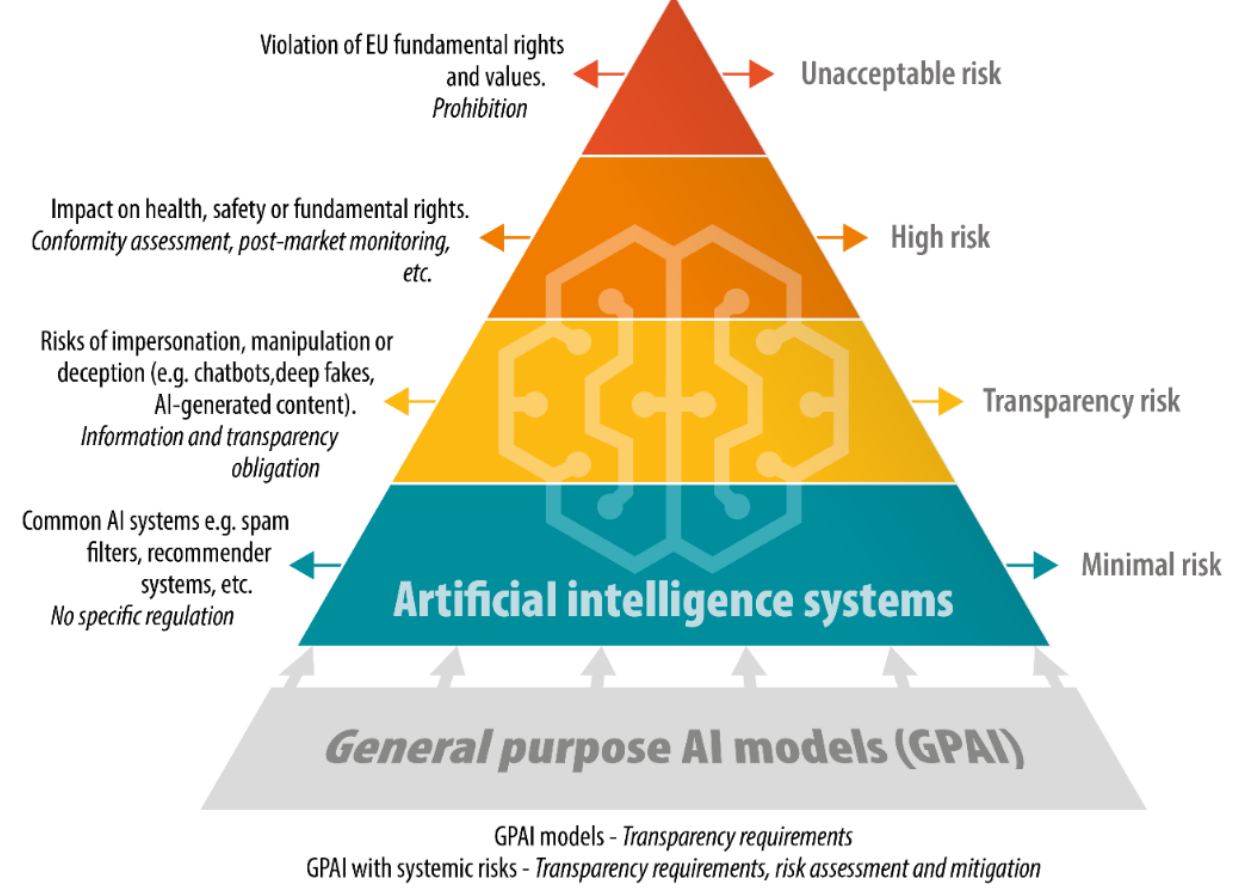
\includegraphics[height=1.5\fontcharht\font`\B]{screen2.png}, which contains six symbols (the Inuktitut writing system is not alphabetic, it is syllabic)\footnote{Using \url{https://www.inuktitutcomputing.ca/Transcoder/index.php} and \url{https://www.compart.com/en/unicode/}}. The corresponding Unicode character numbers (''codepoints'') are: U+1403, U+14C4, U+1483, U+144E, U+1450, U+1466. These are given as \emph{hexadecimal numbers}, using a base of 16 with digits from 0 to F. In text documents this may be written as \textbackslash u1403 \textbackslash u14c4 \textbackslash u1483 \textbackslash u144e \textbackslash u1450 \textbackslash u1466 when the document is read/parsed by an appropriate software tool that can understand this way of writing Unicode characters. 

The corresponding decimal (base 10, with digits from 0 to 9) Unicode character numbers are 5123, 5316, 5251, 5198, 5200, 5222. These are used when the text is written for web content in HTML as HTML entities, such as ''\&amp;\#5123; \&amp;\#5316; \&amp;\#5251; \&amp;\#5198; \&amp;\#5200; \&amp;\#5222;''.

Using UTF-8, each of these six characters can be encoded in 3 bytes. These are usually written in hexadecimal form, indicated by the ''0x'' prefix. Hexademical form is a base 16 system and uses ''numbers'' between 0 and F, that is, it uses 0, 1, 2, 3, 4, 5, 6, 7, 8, 9, A, B, C, D, E, and F as numbers. For example, 0xE1 is 14 (the ''E'') times 16 (the first digit) + 1 times 1 (the second digit), yielding 225. 0x. 

The sequence of Unicode characters for the word ''Inuktitut'' becomes 0xE1 0x90 0x83 (first symbol) 0xE1 0x93 0x84 (second symbol) 0xE1 0x92 0x83 (third symbol) 0xE1 0x91 0x8E (fourth symbol) 0xE1 0x91 0x90 (fifth symbol) 0xE1 0x91 0xA6 (sixth symbol). 

As a business analyst, you may come across data that contains Unicode characters either spelled out in the ''\textbackslash uXXXX'' form, or UTF-8 encoded in byte sequences, or in the HTML format. While you do not need to understand the technical details of Unicode and its different encodings, you should be aware that data in this format is common and you need to know how to deal with it when you encounter it. This includes using a Unicode-aware data storage and management system, using a Unicode-aware business analytics tool, and using a Unicode-aware visualization or report-writing tool.

\begin{tcolorbox}[colback=code]
\subsubsection*{Hands-On Exercise}
\begin{itemize}
	\item Choose your favourite emoji
	\item Determine its Unicode number (''codepage'')
	\item Determine its UTF-8 encoding
\end{itemize}
\end{tcolorbox}

\subsubsection*{Dates and Times}

The world has largely standardized on the Gregorian calendar for secular and commercial use, while other calendar systems exist now only for religious or traditional purposes. However, as with written numbers, written dates show a bewildering variety of forms, depending on the locale and other traditions.

Complexities are introduced by 12 hour (AM/PM) versus 24 hour time formats (''14:30'' is ''2:30PM''), different time zones across the world, leap seconds and leap years, week numbering (does it start with the first full week?), different written formats for the sequence of days, months, and years (is ''06-07-09'' June 7, 2009 or July 6, 2009, or July 9, 2006?), different separators between years, dates, and months (''06/07/09'' and ''06-07-09''), and the difficult arithmetic when using years, months, and days. 

The ISO 8601\footnote{\url{https://en.wikipedia.org/wiki/ISO_8601}} (first published in 1988) and RFC 3339\footnote{\url{https://datatracker.ietf.org/doc/html/rfc3339}} (published in 2002) standards define how dates\index{Date} and times\index{Time} should be written. Table~\ref{tab:iso8601} shows a summary of the ISO 8601/RFC3339 rules (the italicized forms are in ISO 8601 but not in RFC 3339). However, these standards are by no means universally followed and reading/parsing date and time data remains a difficult and complex task in many business analytics settings. 

Even within the ISO 8601 standard, there are numerous ways to express the same date or time, such that June 13, 2024 can be written as an ordinal date (''2024-165'') or a week date (''2024-W24-4'') and the time of T13:45:30 can be written as ''T13:45.500'' or as ''T1345.500''. 

\begin{tcolorbox}[colback=alert]
For a business analyst, it is important to verify the format of dates and times in any data set, especially when the data comes from different or external sources.
\end{tcolorbox}

\begin{table}
\centering
\renewcommand{\arraystretch}{1.25}

\begin{tabular}{l|l} \hline
	Calendar dates & YYYY-MM-DD  \\ \hline
	\textit{Ordinal dates} & \textit{YYYY-DDD} \\ \hline
	\textit{Week dates} & \textit{YYYY-Www-d} \\ \hline
	\multirow{5}{*}{Times} & Thh:mm:ss.sss \textit{(or Thhmmss.ss)} \\
	& Thh:mm:ss \textit{(or Thhmmss)} \\
	& \textit{Thh:mm.mmm or Thhmm.mmm} \\
	& \textit{Thh:mm or Thhmm} \\
	& \textit{Thh.hhh} \\ \hline
	\multirow{2}{*}{Time Zones} & <time>Z or <time>$\pm$hh:mm or \\
	& \textit{(<time>$\pm$hhmm or <time>$\pm$hh)} \\ \hline
	Combined & <date>T<time> \\
	Periods & PnYnMnDTnHnMnS or P<date>T<time> \\ \hline
\end{tabular} \\ \vspace{.5\baselineskip}

\small The \textit{italicized} forms are in ISO 8601 but not in RFC 3339
\caption{ISO 8601 / RFC 3339 Rules for Dates and Times}
\label{tab:iso8601}
\end{table}

\begin{tcolorbox}[colback=alert]
A year is a leap year if it can be divided by four and (cannot be divided by 100 but can be divided by 400). Formally: \\
\small
\texttt{(year \% 4 == 0) and (year \% 100 != 0 or year \% 400 == 0)}
\normalsize
\end{tcolorbox}
 
\begin{tcolorbox}[colback=code]
\paragraph*{Hands-On Exercise} 

\textit{\textbf{\vspace{3mm} \\The territory of Nunavut was created on April 1st, 1999. \vspace{3mm}}}

\begin{itemize}
	\item Express the date in RFC 3339
	\item Calculate the number of days since the creation of Nunavut
	\item Assume that a ceremony took place at 3PM that day in Iqaluit and express this date-time in RFC 3339
	\item Assume the ceremony lasted for 125 minutes and express this duration in RFC 3339
\end{itemize}
\end{tcolorbox}

\subsubsection*{Collections}

Collections\index{Collection (data type)} can store multiple instances of primitive data, often heterogeneous. Different collection types have different characteristics in terms of whether they are 

\begin{itemize}
\item ordered or unordered, 
\item homogeneous (same primitive types) or heterogeneous (different primitive types), 
\item unique or allow duplicates, 
\item mutable (can be changed) or immutable (cannot be changed). 
\end{itemize}

Different software tools offer different kinds of structured types and unfortunately the terminology is not necessarily consistent across software tools. Table~\ref{tab:structured} provides a summary of structured types in Python and R, with examples and key characteristics of the type.

\begin{table}
\renewcommand{\arraystretch}{1.25}
\footnotesize
\centering

\begin{tabular}{l|l|l} \hline
\multicolumn{3}{c}{\textbf{Python}} \\ \hline
list\index{List (in Python)} & \texttt{[1, 2, "a", "b", 2]} & mutable, ordered \\
tuple\index{Tuple (in Python)} & \texttt{(1, 2, "a", "b", 2)} & immutable \\
set\index{Set (in Python)} & \texttt{\{1, 2, "a", "b"\}} &  mutable, unordered, unique \\
dict\index{Dictionary (in Python)} & \texttt{\{"make": "Ford", "year": 2023\}} & mutable \\ \hline
\multicolumn{3}{c}{\textbf{R}} \\ \hline 
list\index{List (in R)} & \texttt{list(1, 2, "a", "b", 2)} & mutable, ordered \\
vector\index{Vector (in R)} & \texttt{c(1, 2, 3)} & mutable, same primitive type \\
factor\index{Factor (in R)} & \texttt{as.factor(c("Hot", "Med", "Cold"))} & ordered\\
matrix\index{Matrix (in R)} & \texttt{matrix(c(1, 2, 3, 4), nrow=2)} & \\
array\index{Array (in R)} & \texttt{array(c(1, 2, 3), c(4, 5, 6))} \\ \hline
\end{tabular}
\caption{Structured data types (''collection types'') in Python and R}
\label{tab:structured}
\end{table}

\FloatBarrier
\subsection{Structured Data}

Data that you encounter in business analytics is built on the primitive and collection data types described in the previous section. We distinguish between structured data, such as tables, key-value pairs, documents, or graphs, and unstructured data, such as text, images, and audio/video data. The latter are called unstructured because these data essentially come as simply a sequence of characters or bytes. Information must first be identified in them and extracted from them, before it can be used for analytics. 

\subsubsection*{Tables}

Table data\index{Table} refers to a method of organizing data in a structured, tabular format, where the data is arranged in rows and columns. Each \emph{row} in a table represents a single record or entry. For instance, in a table of customer data, each row could represent a different customer. \emph{Columns}, sometimes called \emph{fields}, represent different attributes or characteristics or features of a record. In the customer data example, columns might represent attributes of a customer such as their name, address, and purchase history. The intersection of a row and a column is called a cell. Each \emph{cell} contains a single piece of data for a particular attribute of a record. For example, the cell at the intersection of the ''Name'' column and the third row might contain the name of the third customer. Cells may be of simple type or be themselves of structured types, such as sets or lists or even other tables. Tables often have a \emph{header row} at the top, which contains the names of the columns. These headers provide context for what each column in the table represents. Table~\ref{tab:exampletable} shows an example table with a header row that names the columns, three rows of data in three columns that use simple data types (strings and integers). Some tables may also have an \emph{index column} as the first column with row numbers. 

\begin{table}[b]
\centering
\renewcommand{\arraystretch}{1.25}

\begin{tabular}{l|r|r} \hline
\textbf{Name} & \textbf{Area} & \textbf{Population} \\ \hline
Canada & 9,984,670 & 38,781,292  \\
Nigeria & 923,768 & 223,804,632 \\
Germany & 357,600 & 83,294,633 \\ \hline
\end{tabular}
\caption{Example Table}
\label{tab:exampletable}
\end{table}

\paragraph*{CSV Files}

While table data is familiar from spreadsheet systems such as Microsoft Excel or LibreOffice Calc, these tools often store table data in a format that is unique to their system and difficult to read with other tools. This is because spreadsheet tables can contain formulas, formatting instructions such color and font, and other information besides the actual data.

The standard format for storing and exchanging tabular data (i.e. the \emph{serialization format}) is the comma-separated value file (''CSV'' file) \index{Comma-separated values}\index{CSV|see{Comman-separated values}} that is standardized in RFC 4180\footnote{\url{https://datatracker.ietf.org/doc/html/rfc4180}}. Tabular data is stored in a plain text format, without formatting instructions or formatting information, that makes it easy to read and write with different software tools, such as statistics and analytics software, spreadsheet applications, or database management systems. 

CSV files are plain text files, typically encoded in ASCII or UTF-8. Every line contains one row of the table, and fields within a row are separated by commas (although sometimes other, non-standard delimiters such as semicolon are used). Fields are typically of a primitive data type although the interpretation of the field content is left to the software tool reading the CSV file. The CSV file may contain an optional header as the first line, with the same format as the data lines of the file. Every line is ended by a line break using the sequence of  \texttt{CR} and \texttt{LF} characters\footnote{These stand for ''carriage return'' and ''line feed'', respectively, and are a hold-over from the era of mechanical typewriters where the paper carriage needed to be returned to the start of a line and then advanced by one line. \texttt{CR} and \texttt{LF} are represented by ASCII/UTF-8 codes 13 and 10, respectively. Hence, the CSV line break conforms to the Microsoft Windows convention of line breaks. MacOS and Linux use only the LF character for line breaks.}. Every line must contain the same number of fields and fields are allowed to be empty, but must still be separated by a comma. The content of each field may be enclosed by double quotes (although sometimes other, non-standard quotes like single quotes are used). The following is a CSV serialization of Table~\ref{tab:exampletable}:

\begin{textcode}
"Name", "Area", "Population" CR LF
"Canada", "9984670", "38781292" CR LF
"Nigeria", "923768", "223804632" CR LF
"Germany", "357600", "83294633" CR LF
\end{textcode}

While the CSV format is standardized, not all data sets necessarily conform fully to the standard. You may encounter different field delimiters, such as semicolons, tabs, carets (''\^{}'') or others. Line breaks may not use the Microsoft Windows convention of \texttt{CR LF} but instead use only the \texttt{LF} character as is typical on MacOS and Linux/Unix systems. Not all fields may be quoted and you may encounter a mix of double quotes and single quotes even in the same CSV file. Additionally, the field contents themselves, such as numbers and dates, may themselves not be standards compliant and exhibit a range of different notations, as discussed above. For a business analyst, it is important to recognize these variations and be able to address them prior to further data analysis.

\begin{tcolorbox}[colback=code]
\subsubsection*{Hands-On Exercise} 

\begin{itemize}
	\item Search the internet for a CSV file of the population and areas of all countries of the world
	\item Examine the CSV file and answer the following questions:
	\begin{itemize}
		\item What is the delimiter?
		\item Which fields are quoted, and how?
		\item What is the line ending character(s)?
		\item What is the number format?
		\item What is the date format (if there are dates)?
	\end{itemize}
	\item Import the CSV file into your favourite spreadsheet tool
	\begin{itemize}
		\item Does it recognize all information correctly? If not, what is not imported well?
	\end{itemize}
	\item Export the CSV file from your tool under a different name.
	\begin{itemize}
		\item Do you get an identical file to the one you imported? If not, what has changed?
	\end{itemize}
\end{itemize}
\end{tcolorbox}

\paragraph*{Relational Databases}

Tabular data is also the basis for relational database management systems (RDBMS). Tables in these systems are called relations\footnote{After the mathematical concept of a relation as a subset of a cross-product.}\index{Relation}\index{Relational database management system}. Records, i.e. rows of a relation, are uniquely identified by \emph{primary keys}\index{Primary key}. These may be ''natural'' primary keys, such as a combination of fields (also called ''attributes'' in RDBMS) or artificial/synthetic primary keys. For example, in some applications one may assume that the combination of first name, last name, date of birth, and postal code uniquely identifies a person and is used as a primary key. However, it is generally safer to assign artificial primary keys, such as consecutive numbers, to records. 

One key characteristic of data in an RDBMS is that fields in one table can refer to primary key fields in another table. For example, the product numbers for an order in the order table must refer to product numbers of products in the products table. The referring fields are called ''\emph{foreign keys}''. Foreign-key relationships ensure \emph{referential integrity}\index{Referential integrity}\index{Foreign-key relationship}, a form of validity of the data. They also allow an RDBMS to easily retrieve related records from different relations. Figure~\ref{fig:relationkeys} shows an example of keys in a relational database.

\begin{figure}
\centering
\includegraphics[height=1.5in]{Relational_key.png}

\scriptsize{\url{https://commons.wikimedia.org/wiki/File:Relational_key_SVG.svg}}
\caption{Keys in a relational database}
\label{fig:relationkeys}
\end{figure}

Data \emph{normalization}\index{Normalization (in a relational database management system)} in an RDBMS refers to reducing data redundancy. For example, if a customer can have multiple addresses, rather than using multiple address fields in the customer relation or having multiple customer records for a customer (one for each address), normalization will create a table to store addresses where each address refers back to a particular customer using a foreign-key relationship. Normalizing the relations and thereby reducing redundancy makes data storage more efficient and also reduces the potential for inconsistent data, leading to higher data integrity. RDBMS typically use the structured query language (SQL) for retrieving information. 

Prominent RDBMS examples are Oracle RDBMS\footnote{\url{https://www.oracle.com/ca-en/database/}}, a proprietary system for on-premises installation; the PostgreSQL\footnote{\url{https://www.postgresql.org/}} open-source RDBMS system for on-premises installation; and Amazon RDS\footnote{\url{https://aws.amazon.com/rds/}}, Google BigQuery\footnote{\url{https://cloud.google.com/bigquery}}, and Azure SQL\footnote{\url{https://azure.microsoft.com/en-ca/products/azure-sql/database}} which are cloud-based systems on AWS, Google Cloud, and Microsoft Azure, respectively.

\begin{tcolorbox}[colback=code]
\subsubsection*{Hands-On Exercise} 

\begin{itemize}
	\item Assume that products are identified by a product code and have attributes such as description, weight, and price. 
	\item Assume that suppliers are identified by a supplier number and have attributes such as name and address.
	\item Assume that each product is available from exactly one supplier (but a supplier can supply multiple products).
\end{itemize}

\vspace{.5\baselineskip}
Write example relations and identify foreign-key relationships for referential integrity, similar to Figure~\ref{fig:relationkeys}
\end{tcolorbox}


\subsubsection*{Key-Value Data Stores}

Key-value data stores\index{Key-value data store} are a type of non-relational (NoSQL\footnote{NoSQL is term to describe non-relational database models. It does not mean ''no SQL'', but means ''Not only SQL.''}) database that organize data as a collection of key-value pairs. In this model, each data item is stored as a key, along with an associated value. Keys may have multiple components, in an ordered list of ''\emph{minor keys}''. The associated value is not interpreted by the data store, and can contain anything that is meaningful to the application, from primitive data types to collections to complex documents to images or video data. Figure~\ref{fig:keyvalue} shows an example of the key-value model of data storage.

\begin{figure}[h]
\centering
\includegraphics[height=1.25in]{KeyValue.png}
\scriptsize{\url{https://commons.wikimedia.org/wiki/File:KeyValue.PNG}}
\caption{Key Value Data Store}
\label{fig:keyvalue}
\end{figure}

Important characteristics of key-value stores the extremely simple data model: every item is stored as a key and its corresponding value. The keys are unique identifiers. Due to their simple structure, key-value databases allow faster data insertion, updating, and retrieval when compared to more complex relational databases. Unlike relational databases, key-value stores do not have predefined relations with foreign-key relationships. This means that the values associated with keys can be changed dynamically, and different keys can have values of different types. This makes key-value stores more flexible than other databases. On the other hand, they lose the data integrity advantages that come from a predefined schema and the referential integrity based on relationships between multiple tables. Key-value stores are more efficient at storing information than RDBMS because empty table cells do not need to be stored. Key-value stores are also easier to scale and distribute among multiple computers, due to their simple data model. On the other hand, key-value stores are limited in terms of their data querying and analysis capabilities. They are not inherently designed for complex queries, such as joining data across different keys. 

Example key-value data stores include Redis\footnote{\url{https://redis.io/}}, an open-source, in-memory key-value store. Amazon DynamoDB\footnote{\url{https://aws.amazon.com/dynamodb/}} is a proprietary scalable NoSQL database service available on the AWS cloud. Google BigTable\footnote{\url{https://cloud.google.com/bigtable}} and Azure CosmosDB\footnote{\url{https://cosmos.azure.com/}} are key-value stores offered on the Google cloud and the Microsoft Azure cloud. Facebook's RocksDB, Google's LevelDB\footnote{\url{https://github.com/google/leveldb}} and the Apache Cassandra\footnote{\url{https://cassandra.apache.org/}} and HBase\footnote{\url{https://hbase.apache.org/}} projects offer open-source systems for on-premises installation.

\subsubsection*{Documents (JSON)}

When speaking about documents in the context of structured data, we do not mean unstructured text (as a series of characters) but a structured collection of elements. The JavaScript Object Notation (JSON)\index{JavaScript object notation}\index{JSON|see{JavaScript object notation}} is a lightweight data-interchange format that is easy for humans to read and write, and also easy for machines to parse and generate. It is software tool independent. Originally developed for exchanging data between web servers and web browser client applications, it has emerged as a popular way of describing and exchanging many different kinds of data for a variety of purposes in many different applications. JSON was standardized in RFC 8259\footnote{\url{https://datatracker.ietf.org/doc/html/rfc8259}} in 2017.

JSON documents are plain text documents encoded in UTF-8 and consist of key-value pairs where the key or name is a string and the separator is a colon. Values may be strings (enclosed by single or double quotes), numbers, boolean values (''\texttt{true}'' or ''\texttt{false}''), or the special value ''\texttt{null}''. Values are either objects or arrays. \emph{JSON objects} are unordered collections of zero or more key-value pairs and are delimited by ''\{'' and ''\}''. Figure~\ref{fig:json1} shows an example of a JSON object with key-value pairs and nested objects. \emph{JSON arrays} are ordered sequences of zero or more values and are delimited by ''['' and '']''. Arrays contain values but no keys and, because they are ordered, elements can be accessed by position. Figure~\ref{fig:jason2} shows an example of a JSON array, i.e. a list of values, in this example a list of objects.

\begin{figure}[h]
\begin{jsoncode}
{
  "Image": {
    "Width": 1060,
    "Height": 400,
    "Title": "Skyline of Iqaluit, Nunavut",
    "Url": 
"https://upload.wikimedia.org/wikipedia/commons/b/b4/Iqaluit_skyline.jpg",
    "Legal": {
      "Copyrighted": true,
      "License": "GNU Free Documentation License",
      "Inception": "2010-03-24",
      "Author": "Aaron Lloyd"
     },
  }
}
\end{jsoncode}
\caption{JSON Example -- Complex Object}
\label{fig:json1}
\end{figure}

\begin{figure}
\begin{jsoncode}
[
  {
    "Latitude":  56.536389,
    "Longitude": -61.718889,
    "City":      "Nain",
    "Province":  "NL",
    "Postal":    "A0P",
    "Country":   "Canada"
  },
  {
    "Latitude":  53.512778,
    "Longitude": -60.135556,
    "City":      "Sheshatshiu",
    "Province":  "NL",
    "Postal":    "A0P",
    "Country":   "Canada"
  }
]
\end{jsoncode}
\caption{JSON Example -- List of Objects}
\label{fig:jason2}
\end{figure}

\begin{tcolorbox}[colback=code]
\subsubsection*{Hands-On Exercise} 

Describe yourself in a JSON object:
\begin{itemize}
	\item Identify information about yourself, such as names, addresses, dates, relationships (work, school, uni), etc.
	\item Structure the information in JSON Objects and Arrays 
	\item Use nested structures, e.g. objects in arrays, or arrays in objects, or objects in objects, etc.
\end{itemize}
\end{tcolorbox}

\subsubsection*{Documents (XML)}

XML\footnote{\url{https://www.w3.org/TR/2008/REC-xml-20081126/}}, for ''eXtensible Markup Language''\index{Extensible markup language}\index{XML|see{Extensible markup language}}, is a flexible and versatile serialization format that plays an important role in the storage and transmission of data. It is a text-based format that allows for the creation of custom tags (tags are used to describe and delimit data elements), providing a means to define and structure data in a way that is both machine-readable and human-readable. Unlike HTML (the Hypertext Markup Language that describes web pages), which has a predefined set of tags for web page layout, XML does not prescribe any specific tags, allowing users to create tags tailored to their specific application.

XML's development began in the late 1990s by an XML Working Group under the auspices of the World Wide Web Consortium (W3C). XML 1.0 was officially recommended by the W3C in February 1998. It quickly gained widespread adoption due to its simplicity, extensibility, and ability to work seamlessly across different systems and platforms. XML has become a cornerstone technology in numerous domains, from web services and APIs to configuration files and data interchange formats.

An XML document is composed of \emph{elements}\index{Element (in XML)}. XML elements are described by matching opening and closing \emph{tags}\index{Tag (in XML)}, between which simple text content or other XML elements may be placed. Elements in turn may have \emph{attributes}\emph{Attribute (in XML)}. Attributes are specified in the opening tag of an element and may contain simple, quoted text data only. This hierarchical organization can represent complex data relationships and nested structures. 

XML files are human-readable and self-descriptive in nature; the names of elements and attributes used in the document indicate that type or meaning of the data they describe, enhancing the understanding and interpretation of the data's structure and meaning. Additionally, XML is platform-independent and language-neutral, making it a universally accepted standard for data interchange across different systems and applications. 

XML element and attribute names may be defined within a \emph{namespace}\index{Namespace (in XML)}. This allows mixing elements with the same name but different namespaces in the same document and removes ambiguity that could arise from identically named elements that describe different data or content. For example when mixing customer and product information in an order document, both the customer and the product may have a ''name'' element and different namespaces for the two ''name'' elements helps to tell them apart. Namespaces are declared using the special \texttt{xmlns} attribute and are typically defined by a URI (Uniform Resource Identifier), typically a URL (Uniform Resource Locator). These URI/URL are for identification purposes and do not need to describe an actually existing resource.

The following example describes the Innu people of northern Canada in the form of an XML document. The element names, like \texttt{People, History, Culture} are self-descriptive and human-readable. Note that each opening tag (such as \texttt{<Traditions>}) is matched by a corresponding closing tag (such as \texttt{</Traditions>}. Empty elements that do not contain any content are defined using a single tag (for example, the \texttt{<geo:Location.../>} element). Some elements contain attributes, such as the \texttt{Name} attribute of the \texttt{GeneralInformation} element. Attributes must be quoted character strings.

Namespaces are declared at the root element of the document: The \texttt{xmlns:geo} and \texttt{xmlns:hist} are namespace declarations. They are used to distinguish between geographical (geo) and historical (hist) data. Notice how element and attribute names may be prefixed by a namespace (such as the \texttt{<hist:History>} element or the \texttt{geo:Country} attribute. The \texttt{xmlns} declaration defines the default namespace that applies to all elements and attributes without an explicit namespace.

Notice that elements with the same name may be repeated. For example, there are multiple \texttt{Period} elements in the \texttt{History} element, each with their own \texttt{hist:era} attribute to specify the era. This allows one to represent lists or sets of elements. 

\begin{samepage}
\begin{xmlcode}
<People
      xmlns="https://www.example.com/peoples"
      xmlns:geo="http://www.example.com/geo" 
      xmlns:hist="http://www.example.com/history">
    <GeneralInformation 
            Name="Innu" Language="Innu-aimun">
        <geo:Location geo:Country="Canada" 
                  geo:Regions="Labrador, Quebec" />
    </GeneralInformation>
    <hist:History>
        <hist:Period hist:era="Pre-Colonial">
            <Description>
                Nomadic lifestyle, primarily 
                hunting and fishing.
            </Description>
        </hist:Period>
        <hist:Period hist:era="Post-Colonial">
            <Description>
                Impact of colonization, 
                including displacement and 
                cultural changes.
            </Description>
        </hist:Period>
    </hist:History>
    <Culture>
        <Traditions>
            <Tradition>
                Hunting and fishing as cultural 
                and subsistence activities.
            </Tradition>
            <Tradition>
                Use of the tepee for temporary 
                shelter.
            </Tradition>
        </Traditions>
        <Art>
            <Form>Drum making</Form>
            <Form>Clothing with intricate beadwork
            </Form>
        </Art>
    </Culture>
    <Challenges>
        Issues like land rights, cultural preservation
    </Challenges>
</People>
\end{xmlcode}
\end{samepage}

Given the similarities between JSON and XML it is not surprising that one can readily be transformed into the other. An equivalent JSON document of the above XML document could be as follows:

\begin{samepage}
\begin{jsoncode}
"Innu": {
	"@xmlns:geo": "http://www.example.com/geo",
	"@xmlns:hist": "http://www.example.com/history",
	"GeneralInformation": {
		"@Name": "Innu",
		"@Language": "Innu-aimun",
		"Location": {
			"@geo:Country": "Canada",
			"@geo:Regions": "Labrador, Quebec"
		}
	},
	"History": {
		"Period": [
			{
				"@hist:era": "Pre-Colonial",
				"Description": "Nomadic lifestyle, 
				     primarily hunting and fishing."
			},
			{
				"@hist:era": "Post-Colonial",
				"Description": "Impact of colonization, 
				     including displacement and 
				     cultural changes."
			}
		]
	},
	"Culture": {
		"Traditions": {
			"Tradition": [
				"Hunting and fishing as cultural and 
				     subsistence activities.",
				"Use of the tepee for temporary shelter."
			]
		},
		"Art": {
			"Form": [
				"Drum making",
				"Clothing with intricate beadwork"
			]
		}
	},
	"CurrentStatus": {
		"Challenges": "Issues like land rights, 
		     cultural preservation, etc."
	}
}
\end{jsoncode}
\end{samepage}

In this example, XML namespaces are represented as properties with names prefixed by ''@''. This does not imply any special meaning or treatment in JSON, but makes it easier for the computer to read and parse (''understand'') the document. XML elements with attributes are represented as JSON objects, while repeated elements are represented as JSON arrays. 

In comparing XML to JSON, it is evident that both formats are human as well as machine readable. It is also clear that XML is more verbose or lengthy. This is an advantage in that it makes it very self-descriptive, but a disadvantage in that XML documents are larger than corresponding JSON documents. In contrast, JSON is more compact or lightweight, and not quite as self-descriptive as an XML document. XML supports more complex structures than JSON through is attributes, namespaces, and a larger selection of possible data types for simple content. 

While XML can be strictly defined using XML Schema there is not yet a well-adopted means for specifying JSON documents. This means that JSON documents cannot be validated against a set of rules or constraints, possibly leading to data quality issues, but, on the other hand, may be used more flexibly.

\begin{tcolorbox}[colback=code]
\subsubsection*{Hands-On Exercise} 

Describe yourself in an XML document:
\begin{itemize}
	\item Identify information about yourself, such as names, addresses, dates, relationships (work, school, uni), etc.
	\item Structure the information in Elements and Attributes 
	\item Use nested elements where appropriate
\end{itemize}
\end{tcolorbox}

\paragraph*{Document Databases}

Document databases\index{Document database}, a type of NoSQL databases, are designed to store, retrieve, and manage document-oriented information, typically in the form of JSON or BSON (Binary JSON) documents. Unlike traditional relational data\-bases that store data in rows and columns, document databases handle data in a more flexible, semi-structured way. They are designed for handling large volumes of diverse data that does not fit into a tabular format. Document databases may be thought of as nested key-value data stores where all keys are strings. Their fundamental unit of storage is the document. Unlike relational databases, document databases usually do not have a predefined schema. Each document in a collection can have its own unique structure, with different fields, data types, and sizes. This makes them more flexible than RDBMS. Document databases often offer query languages that are designed to handle complex queries on document data, including searching within documents and aggregating data across multiple documents. 

Typical use cases for document databases are content management, where different types of content need to be stored and retrieved efficiently, catalogs and product data, where each product may have different attributes and structures, and real-time analytics of Internet-of-Things (IoT) sensor data, where large volumes of unstructured and semi-structured data are generated.

Prominent examples of document databases are MongoDB\footnote{\url{https://www.mongodb.com/}} and ArangoDB \footnote{\url{https://arangodb.com/}} which are partially proprietary system for on-premises installation or cloud-based use; Apache CouchDB\footnote{\url{https://couchdb.apache.org/}} which is a fully open-source system; and AWS DocumentDB\footnote{\url{https://aws.amazon.com/documentdb/}} which is a cloud-based system on the Amazon AWS cloud. 

\subsubsection*{Graphs}

Graphs\index{Graph} consist of \emph{nodes}\index{Node} (also called \emph{vertices}\index{Vertex|see{Node}}) and \emph{edges}\index{Edge (in a graph)} (also called \emph{arcs}\index{Arc|see{Edge (in a graph)}} or \emph{relationships}\index{Relationship (in a graph)|see{Edge (in a graph}}) that connect two nodes. Edges may be directed or undirected. Both nodes and edges may be labelled or typed. For example, different node types may be used to represent customers and products; different edge types may represent a customer ordering a product, a customer returning a product, a customer obtaining a quote about a product, etc. Graph data is found in social networks (between people, events, topics, etc.), in logistics networks (between suppliers, customers, warehouses, distribution centers, etc.), in financial networks (between organizations, accounts, etc.), in biological networks, and in many other contexts.

\begin{figure}[h]
\centering
\includegraphics[height=2in]{GraphDatabase_PropertyGraph.png}
\scriptsize{\url{https://commons.wikimedia.org/wiki/File:GraphDatabase_PropertyGraph.png}}
\caption{Property Graph Example}
\label{fig:propertygraph}
\end{figure}

Graph data is either in the form of property graphs or RDF graphs (''Resource Description Framework''). \emph{Property graphs} are a graph data model where each node and edge can have a set of properties (key-value pairs) that describe the attributes of the entity represented by the node. Edges can also have properties, which can describe attributes of the relationship. For example, a node representing a person might have properties like \texttt{name: ''John Doe''} and \texttt{age: 30}. An edge representing a friendship relationship might have a property like \texttt{since: 2010}. Property values may be simple data types or complex ones like JSON documents. Figure~\ref{fig:propertygraph} shows an example property graph. 
    
In contrast to property graphs, RDF\footnote{\url{https://www.w3.org/RDF/}} graphs\index{Resource description framework}\index{RDF|see{Resource description framework}} do not allow properties on nodes and edges. Instead, they describe information in subject--predicate--object triples. What might be an ''age'' property in a property graph can be described in RDF as the triple \texttt{JohnDoe -- has age -- 30}. In an RDF graph, subjects and objects have unique identifiers (URIs, uniform resource identifiers\footnote{\url{https://www.w3.org/TR/webarch/\#identification}} that are typically defined in the form of URL as defined in RFC 2616\footnote{\url{https://www.ietf.org/rfc/rfc2616.txt}}), or are literal values such as strings or numbers. Figure~\ref{fig:rdfgraph} shows and example RDF graph.

\begin{figure}[h]
\centering
\includegraphics[height=3in]{rdf.png}
\scriptsize{\url{https://commons.wikimedia.org/wiki/File:Rdf_graph_for_Eric_Miller.png}}
\caption{RDF Graph Example}
\label{fig:rdfgraph}
\end{figure}

While graphs could be modelled or described in table (relational) form, or as key-value pairs, graph databases provide powerful, intuitive, and efficient graph-specific queries\footnote{Source: Wang, Y., Li, Y., Fan, J., Ye, C., \& Chai, M. (2021). A survey of typical attributed graph queries. World Wide Web, 24, 297-346}. Figure~\ref{fig:graphqueries} shows an overview of different query types:

\begin{itemize}
	\item \emph{Path queries}: Reachability of nodes, shortest-path between nodes
	\item \emph{Subgraph queries}: Exact or approximate match of a smaller graph in a larger one
	\item \emph{Aggregate queries}: Aggregating nodes or properties along paths
	\item \emph{Similarity search}: Similarity of nodes or edges using path-based approaches, graph embedding-based approaches
	\item \emph{Keyword search}: Tree-based semantics, subgraph-based semantics
	\item \emph{Natural language query answering}: Identifying edges or nodes
\end{itemize}

\begin{figure}
\includegraphics[width=\textwidth]{screen3.png}
\scriptsize
Source: Wang, Y., Li, Y., Fan, J., Ye, C., \& Chai, M. (2021). A survey of typical attributed graph queries. World Wide Web, 24, 297-346.
\caption{Graph Queries}
\label{fig:graphqueries}
\end{figure}

Prominent examples of graph database management systems are JanusGraph\footnote{\url{https://janusgraph.org/}}, a fully open-source system for on-premises installation; ArangodDB\footnote{\url{https://arangodb.com/}}, Neo4J\footnote{\url{https://neo4j.com/}}, and OrientDB\footnote{\url{https://orientdb.org/}} which are partially open-source for on-premises installation; AWS Neptune\footnote{\url{https://aws.amazon.com/neptune/}} on the Amazon AWS cloud, and CosmosDB\footnote{\url{https://azure.microsoft.com/en-ca/products/cosmos-db}} on Microsoft Azure cloud. 

While there does not exist a standardized serialization format for property graph data interchange, PG-JSON and GraphSON are two recent proposals to describe property graphs in a JSON object, shown in Figure~\ref{fig:pgjson} and Figure~\ref{fig:graphson}.

\begin{figure}[h]
\begin{jsoncode}
{
  "nodes":[
    {
     "id":101,
     "labels":["Person"],
     "properties":{"name":["Alice"], "age":[15], "country":["USA"]}
    },
    {
     "id":102,
     "labels":["Person", "Student"],
     "properties":{"name":["Bob"], "country":["Japan", "Germany"]}
    }
  ],
  "edges":[
    {
     "from":101,
     "to":102,
     "undirected":true,
     "labels":["sameSchool", "sameClass"],
     "properties":{"since":[2012]}
    },
    {
     "from":102,
     "to":101,
     "labels":["likes"],
     "properties":{"since":[2015]}
    }
  ]
}
\end{jsoncode}

\caption{PG-JSON Example}
\label{fig:pgjson}

\end{figure}

\begin{figure}[h]
\begin{subfigure}[c]{0.48\textwidth}
\begin{jsoncode}
{ 
"graph": {
  "mode":"NORMAL",
  "vertices": [
    {
      "name": "lop",
      "lang": "java",
      "_id": "3",
      "_type": "vertex"
    },
    {
      "name": "vadas",
      "age": 27,
      "_id": "2",
      "_type": "vertex"
    },
    {
      "name": "marko",
      "age": 29,
      "_id": "1",
      "_type": "vertex"
    },
    {
      "name": "peter",
      "age": 35,
      "_id": "6",
      "_type": "vertex"
    },
|\ldots|
\end{jsoncode}
\end{subfigure}
\hfill
\begin{subfigure}{0.48\textwidth}
\begin{jsoncode}
  "edges": [
    {
      "weight": 1,
      "_id": "10",
      "_type": "edge",
      "_outV": "4",
      "_inV": "5",
      "_label": "created"
    },
    {
      "weight": 0.5,
      "_id": "7",
      "_type": "edge",
      "_outV": "1",
      "_inV": "2",
      "_label": "knows"
    },
    {
      "weight": 0.400,
      "_id": "9",
      "_type": "edge",
      "_outV": "1",
      "_inV": "3",
      "_label": "created"
    },
|\ldots|
\end{jsoncode}
\end{subfigure}
\caption{GraphSON Example}
\label{fig:graphson}
\end{figure}
\FloatBarrier

In contrast, multiple standardized RDF graph serializations are defined\footnote{Examples taken from \url{https://en.wikipedia.org/wiki/Resource_Description_Framework}}. The ''Turtles'' format (Terse RDF Triples)\index{Terse RDF Triples}\index{Turtles|see{Terse RDF Triples}} is the most compact representation and most easy to read for humans. The following example describes the RDF graph in Figure~\ref{fig:rdfgraph}. It defines three prefixes of URIs to identify resources. These resources form the subjects, predicates, and objects of the RDF triples.

\begin{textcode}
@prefix eric:    <http://www.w3.org/People/EM/contact#> .
@prefix contact: <http://www.w3.org/2000/10/swap/pim/contact#> .
@prefix rdf:     <http://www.w3.org/1999/02/22-rdf-syntax-ns#> .

eric:me contact:fullName "Eric Miller" .
eric:me contact:mailbox <mailto:e.miller123(at)example> .
eric:me contact:personalTitle "Dr." .
eric:me rdf:type contact:Person .
\end{textcode}

\noindent The equivalent N-Triples representation is still reasonably compact, but easier for computers to read and parse. Here, the URI prefixes are embedded in the subjects, predicates, and objects:

\begin{textcode}
<http://www.w3.org/People/EM/contact#me> 
 <http://www.w3.org/2000/10/swap/pim/contact#fullName> 
  "Eric Miller" .

<http://www.w3.org/People/EM/contact#me>
 <http://www.w3.org/2000/10/swap/pim/contact#mailbox> 
  <mailto:e.miller123(at)example> .

<http://www.w3.org/People/EM/contact#me>
 <http://www.w3.org/2000/10/swap/pim/contact#personalTitle> 
  "Dr." .
 
<http://www.w3.org/People/EM/contact#me>
 <http://www.w3.org/1999/02/22-rdf-syntax-ns#type>
  <http://www.w3.org/2000/10/swap/pim/contact#Person> .
\end{textcode}

\begin{samepage}
\noindent Finally, the RDF/XML serialization uses the XML language to describe RDF triples. It is quite verbose: 

\begin{xmlcode}
<?xml version="1.0" encoding="utf-8"?>
<rdf:RDF xmlns:contact="http://www.w3.org/2000/10/swap/pim/contact#" 
xmlns:eric="http://www.w3.org/People/EM/contact#" 
xmlns:rdf="http://www.w3.org/1999/02/22-rdf-syntax-ns#">
  <rdf:Description rdf:about="http://www.w3.org/People/EM/contact#me">
    <contact:fullName>Eric Miller</contact:fullName>
  </rdf:Description>
  <rdf:Description rdf:about="http://www.w3.org/People/EM/contact#me">
    <contact:mailbox rdf:resource="mailto:e.miller123(at)example"/>
  </rdf:Description>
  <rdf:Description rdf:about="http://www.w3.org/People/EM/contact#me">
    <contact:personalTitle>Dr.</contact:personalTitle>
  </rdf:Description>
  <rdf:Description rdf:about="http://www.w3.org/People/EM/contact#me">
    <rdf:type rdf:resource="http://www.w3.org/2000/10/swap/pim/contact#Person"/>
  </rdf:Description>
</rdf:RDF>
\end{xmlcode}
\end{samepage}

\begin{tcolorbox}[colback=code]
\subsubsection*{Hands-On Exercise}

Document yourself in a Turtle:
\begin{itemize}
	\item Identify information about yourself, such as names, addresses, dates, relationships (work, school, uni), etc.
	\item Structure the information in Turtle triples
	\item Make up appropriate prefixes and appropriate verbs/predicates
\end{itemize}
\end{tcolorbox}

\subsection{Unstructured Data}

\subsection*{Text}

Text\index{Text} refers to written language in some writing system and is provided as a string of characters or a file containing bytes that encode the text in Unicode UTF-8 or some other format. Text data in business analytics does not normally contain formatting instructions, such as font sizes or font styles, or mixed tables or images, as might be common in word processing systems. Instead, it refers to plain text only. 

Text analysis is the process of extracting meaningful information from unstructured text data. Typical text analysis tasks are named entity recognition, co-reference analysis, event extraction, sentiment analysis, and document clustering. Named entity recognition identifies names of persons, organizations, or places, and expressions of time, quantity, or monetary amounts in a text. It is useful for content classification and data extraction. 

Co-reference analysis involves identifying when two or more expressions in a text refer to the same entity. This task is crucial for understanding the context and for maintaining the continuity of subjects throughout the text. For example, in the sentence ''Alice drove her car. She parked it near the mall,'' co-reference analysis links ''She'' to ''Alice'' and ''it'' to ''Alice's car.''. Co-reference analysis helps in understanding the text flow and the relationships between various entities.
    
Event and relationship extraction  is about identifying instances of specific types of events in text and the entities associated with them. An event can be anything that happens or is described as happening. For example, in ''The company acquired a startup for \$1 million in 2021,'' event extraction would identify the acquisition event, involving the company, the startup, the amount of \$1 million, and the time 2021. This task is useful for information monitoring or historical data analysis. 

Sentiment analysis involves identifying and categorizing opinions expressed in a piece of text, especially to determine whether the writer's attitude towards a particular topic, product, etc., is positive, negative, or neutral. It is widely used in social media monitoring, brand monitoring, customer service, and market research.

Document clustering is a method to categorize documents into groups (or clusters) based on their similarity. It is useful for news aggregation, organizing web search results, discovering prevalent topics or themes and grouping of similar documents to make it easier to find relevant information.

The history of text mining approaches has evolved through several stages. In the 1950s and 1960s, text mining began with symbolic approaches, involving rule-based systems. These systems, which relied on handcrafted linguistic rules, attempted to encode human language knowledge into a format readable by computers. Their reliance on extensive domain knowledge and manual rule creation made them inflexible and unable to adapt to language variations and new data.

The late 1980s and 1990s saw a shift towards statistical methods in text mining, driven by the growing availability of digital text data and computational power. This period was characterized by the use of machine learning models like Naive Bayes, Decision Trees, and Support Vector Machines. The era of corpus linguistics also emerged, enabled by the availability of large text corpora, allowing for the statistical analysis of real-world text data. Techniques like Latent Semantic Analysis (LSA) and Latent Dirichlet Allocation (LDA) were developed for topic modeling and document classification. 

The 2010s marked a revolution in text mining with the advent of deep learning and neural networks, which provided the ability to learn complex patterns in large datasets. Recurrent Neural Networks (RNNs) and variants like LSTMs became popular for handling sequential text data. The development of attention mechanisms and transformer models in the 2020s, such as Google's BERT or OpenAI's ChatGPT, represented yet another significant advancement.

\begin{tcolorbox}[colback=code]
\subsubsection*{Hands-On Exercises}
 
\begin{enumerate}
	\item Identify a specific business problem that can be addressed by analyzing text data
	\item What text data would you need to address the problem?
	\item What would you wish to do with the text data?
	\item Where might you get this text data?
\end{enumerate}
\end{tcolorbox}

\subsubsection*{Regular Expressions (RegEx)}

Regular expressions (often abbreviated as regex or regexp) are a tool for pattern matching within text\index{Regular expression}\index{Regex|see{Regular expression}}. They enable the specification of complex search patterns in a concise and flexible manner. Regular expressions are widely used for searching, editing, or manipulating text and data. For example, the following regular expression matches any number, including one in scientific notation\footnote{Source: \url{https://en.wikipedia.org/wiki/Regular\_expression}}:

\noindent \mintinline[bgcolor=code,frame=single,framesep=10pt]{text}{
[+-]?(\d+(\.\d*)?|\.\d+)([eE][+-]?\d+)?.}

\begin{table}[h]
\small
\centering

\renewcommand{\arraystretch}{1.25}
\begin{tabularx}{\textwidth}{c|X} \hline
{\bf Metacharacter} & {\bf Description} \\ \hline \hline
\^{ } & Matches start of text \\ \hline
. & Matches any character; matches the dot character when used within brackets \\ \hline
$[$ $]$ & Matches any of the characters in the brackets; - can be used to specify ranges of characters \\ \hline
$[$\^{ } $]$ & Matches any character not in the brackets \\ \hline
\$ & Matches the end of text \\ \hline
( ) & Marked subexpression \\ \hline
\textbackslash n & Matches the n-th marked subexpression \\ \hline
* & Matches the preceding element zero or more times \\ \hline
\{m,n\} & Matches the preceding element at least m and not more than n times \\ \hline
\end{tabularx} \\
\vspace{.5\baselineskip}

{\footnotesize Adapted from \url{https://en.wikipedia.org/wiki/Regular_expression}} 

\caption{Basic Regular Expressions}
\label{tab:regexbasic}
\end{table}

\begin{table}[h]
\small 
\centering

\renewcommand{\arraystretch}{1.25}

\begin{tabularx}{\textwidth}{c|X} \hline
{\bf RegEx} & {\bf Matches} \\ \hline \hline
.at & ''hat'', ''cat'', ''bat'', ''4at'', etc. \\ \hline
$[$hc$]$at & ''hat'', ''cat'' \\ \hline
$[$\^{ }b$]$ & all strings matched by .at except ''bat'' \\ \hline
$[$\^{ }bc$]$ & all strings matched by .at except ''bat'' and ''cat'' \\ \hline
\^{ }$[$bc$]at$ & ''bat'' and ''cat'' at start of text \\ \hline
$[$bc$]at$\$ & ''bat'' and ''cat'' at end of text \\ \hline
\textbackslash $[$.\textbackslash$]$ & any single charater surrounded by $[$ and $]$, e.g. ''$[$a$]$'', ''$[$7$]$'', etc. \\ \hline
s.* & character ''s'' followed by zero or more characters, e.g. ''s'', ''saw'', ''s3w96.7'', etc. \\ \hline
\end{tabularx} \\
\vspace{.5\baselineskip}

{\footnotesize Adapted from \url{https://en.wikipedia.org/wiki/Regular_expression}} 

\caption{Basic Regular Expression Examples}
\label{tab:regexbasicexamples}
\end{table}

Regular expressions are specified using \emph{meta characters}\index{Meta character}, i.e. characters that describe other characters. Table~\ref{tab:regexbasic} shows the metacharacters for basic regular expressions as defined by the POSIX standard. All other characters are treated as literal characters. With these definitions, you can understand the examples shown in Table~\ref{tab:regexbasicexamples}.

Extended regular expressions add optionality and choice operators to set of basic regex meta characters, as shown in Table~\ref{tab:regexex}. Table~\ref{tab:regexexexamples} shows examples for using these operators.

\begin{table}
\small
\centering

\renewcommand{\arraystretch}{1.25}
\begin{tabularx}{\textwidth}{c|X} \hline
{\bf Meta character} & {\bf Description} \\ \hline \hline
? & Matches preceding element zero or one time \\ \hline
+ & Matches preceding element one or more times \\ \hline
| & Matches either the expression before or after the choice operator \\ \hline
\end{tabularx} \\
\vspace{.5\baselineskip}

{\footnotesize Adapted from \url{https://en.wikipedia.org/wiki/Regular_expression}}

\caption{Extended Regular Expressions}
\label{tab:regexex}
\end{table}

\begin{table}
\small
\centering
\renewcommand{\arraystretch}{1.25}

\begin{tabularx}{\textwidth}{c|X} \hline
{\bf RegEx} & {\bf Matches} \\ \hline \hline
$[$hc$]$?at & ''at'', ''hat'', ''cat'' \\ \hline
$[$hc$]$*at & ''at'', ''hat'', ''cat'', ''chat'', ''chchchat'', etc. \\ \hline
$[$hc$]$+at & ''hat'', ''cat'', ''chat'', ''chchchat'', etc. \\ \hline
cat | dog & ''cat'' or ''dog'' \\ \hline
\end{tabularx}  \\
\vspace{.5\baselineskip}

{\footnotesize Adapted from \url{https://en.wikipedia.org/wiki/Regular_expression}} 

\caption{Extended Regular Expression Examples}
\label{tab:regexexexamples}
\end{table}

Over the years, different types or ''dialects'' of regular expressions have been developed for or within different programming languages. One popular dialect is that used in the Perl programming language or the Vim text editor. One important way in which they differ is in the character classes they provide as shortcuts for specifying a set of characters to match. Table~\ref{tab:regexclasses} shows an excerpt of the most frequently used character classes. 

\begin{table}
\small
\centering
\renewcommand{\arraystretch}{1.25}
\begin{tabular}{l|l|l|l} \hline
                  & \textbf{Perl/Vim} & \textbf{ASCII} & \textbf{POSIX} \\ \hline \hline
Digits            & \textbackslash d & [0-9]  & [:digit:]  \\
Non-digits        & \textbackslash D & [\textasciicircum 0-9] & \\
Lowercase letters & \textbackslash l & [a-z] & [:lower:] \\
Uppercase letters & \textbackslash u & [A-Z] & [:upper:] \\
Alphanumeric chars & \textbackslash w & [A-Za-z0-9\_] & \\
Non-word chars    & \textbackslash W & [\textasciicircum A-Za-z0-0\_] & \\
Whitespace        & \textbackslash s & [ \textbackslash t\textbackslash r\textbackslash n\textbackslash v\textbackslash f] & [:space:] \\
Non-whitespace    & \textbackslash S & [\textasciicircum{ } \textbackslash t\textbackslash r\textbackslash n\textbackslash v\textbackslash f] & \\ \hline
\end{tabular}
\caption{Character classes in Regular Expressions}
\label{tab:regexclasses}
\end{table}

Regular expressions are a fundamental tool in text processing and manipulation, offering a robust and efficient method for pattern matching and string analysis. Their versatility makes them an essential skill in many programming and data-related tasks. Regular expressions are available in all programming languages and statistics and analytics software tools and allow a basic level of text processing and manipulation.

\begin{tcolorbox}[colback=code]
\subparagraph*{Hands-On Exercise} 
\begin{enumerate}
	\item Specify a RegEx to match Canadian postal codes:
\end{enumerate}
\url{https://www.canadapost-postescanada.ca/cpc/en/support/articles/addressing-guidelines/postal-codes.page} 
\begin{enumerate}
	\setcounter{enumi}{1}
	\item Specify a RegEx to match a full RFC 3339 date with timezone, such as ''2023-11-14T20:42:53-04:30''
	\item \emph{Challenge}: Specify a RegEx that matches any ISO 8601 date-time format
\end{enumerate}
\end{tcolorbox}

\subsubsection*{Levenshtein Distance}

The Levenshtein distance\index{Levenshtein distance} is a metric of similarity of two text fragments. It is a type of string--edit distance, in that it measures the lowest number of \emph{insertion}, \emph{deletion} and \emph{substitution} operations of individual characters to transform one text fragment into the other. The operations may be equally weighted or be differentially weighted, for example to penalize deletion operations more than insertion operations. The recursive definition is shown in Figure~\ref{fig:levenshtein}. 

As an example, consider the two strings ''kitten'' and ''sitting''. The (unweighted) Levenshtein distance between the two is 3. In the first edit, the ''k'' is substituted with an ''s'', then the ''e'' is substituted with an ''i'' and finally a ''g'' is inserted at the end.

\begin{figure}
\centering
\includegraphics[width=0.75\textwidth]{screen6.png} \\

\scriptsize
\url{https://en.wikipedia.org/wiki/Levenshtein_distance}
\caption{Levenshtein Distance}
\label{fig:levenshtein}
\end{figure}


\begin{tcolorbox}[colback=code]
\subparagraph*{Hands-On Exercise} 
Determine the Levenshtein distances between the following:
\begin{enumerate}
  \item Last five digits of your student number and ''12345''
  \item The words ''Nunavut'' and ''Nunatsiavut''
  \item The words ''Inuktitut'' and ''Innuttitut''
  \item The words ''Mikak'' and ''Micock''
\end{enumerate}
\end{tcolorbox}


\subsection*{Images}

Image data is the representation of visual information in a digital format.There are two primary types of image formats: vector and raster. 

\begin{wrapfigure}{l}{1.5in}
\begin{center}
\includegraphics[height=1in]{Persian_sand_CAT.jpg}
\scriptsize\url{https://commons.wikimedia.org/wiki/File:Persian_sand_CAT.jpg}
\end{center}
\end{wrapfigure}

Vector images\index{Image!Vector}\index{Vector image|see{Image!Vector}} represent images as sets of graphical primitives such as lines, polygons, and curves (vectors) using their mathematical description. Common vector image formats are SVG\footnote{\url{https://www.w3.org/TR/SVG2/}} (Scalable Vector Graphics), PDF (Portable Document Format) and EPS (Encapsulated Postscript). Vector images can be scaled to any size without losing quality, as the mathematical formulas for the graphical primitives adapt and scale to the new size.

Raster images\index{Image!Raster}\index{Raster image|see{Image!Raster}} are composed of a grid of pixels (''picture element''), where each pixel has a color value. These are also known as bitmap images. The quality of raster images is dependent on their resolution. Scaling up a raster image can lead to a loss in quality, known as pixelation. Common formats are JPEG, and PNG, which use a lossy compression, that is, in reducing the file size, image detail may be lost. In contrast, the TIFF format uses lossless compression, retaining the full information of an image. 

Image data in analytics is typically in a raster format using the RGB colorspace, which describes colours in terms of their red, green, and blue components\footnote{Another widely used colour space is CMYK, where a pixel's color is described in terms of its cyan, magenta, yellow, and black components.}. Hence, each pixel is described by 3 bytes (color components range from 0 to 255) and a full image can be thought of conceptually as  a $3 \times X \times Y$ array of values between 0 and 255. For image analytics, images in a compressed format such as JPEG, PNG or TIFF must be decompressed to the full set of $X \times Y$ pixels, and the three RGB values are usually scaled to a range between 0 and 1.

Typical image analysis tasks include object detection and counting, object classification, image segmentation, and image retrieval. Object classification or image classification categorizes an entire image, or specific objects within an image, into predefined classes. This is commonly used for social media analysis or applications like photo tagging. Object detection involves identifying and locating objects within an image. This task goes beyond merely recognizing what objects are present; it also determines where they are in the image. Typically, object detection algorithms output a bounding box for each detected object, specifying its coordinates within the image. Object detection is widely used in applications such as surveillance, face detection, and autonomous vehicles. Image segmentation divides an image into multiple segments with the aim of simplifying or changing the representation of an image into a form that is more meaningful and easier to analyze. Image segmentation is used in medical imaging, machine vision, and object tracking. Image retrieval involves searching and retrieving images from a large database based on the content of the images themselves. It typically involves extracting features like color, texture, and shape from the images and using these features to find similar images in a database. 

Business applications of image analysis include robotics, character and handwriting recognition in documents for process automation, security (identity verification, fraud detection, etc.) and manufacturing (defect detection, etc.).

\begin{tcolorbox}[colback=code]
\subsubsection*{Hands-On Exercise} 

\begin{enumerate}
	\item Identify a specific business problem that can be addressed by analyzing image data
	\item What image data would you need to address the problem?
	\item What would you wish to do with the image data?
	\item Where might you get this image data?
\end{enumerate}
\end{tcolorbox}

\subsection*{Video}

Video data consists of a sequence of images (''frames'') displayed at a certain rate (frame rate) to create the illusion of motion. Accompanying audio tracks are synchronized with these frames. Video data can be complex due to the need to balance quality, resolution, compression, and file size. Conceptually, video is a series of image \emph{frames} in raster image format, i.e. a $T \times 3 \times X \times Y$ array of RGB values between 0\ldots255 (where $T$ refers to the set of frames over time).

However, in practice, video data is heavily compressed in video files as specified by different video formats. Each format has its compression techniques and algorithms, impacting the video's quality, size, and playback compatibility. A video \emph{codec} (compressor-decompressor) is a software or hardware tool that compresses (encodes) and decompresses (decodes) digital video in a particular format to reduce file size and bandwidth requirements for storage or transmission. Popular video formats (codecs)\index{Video codec} are H.264, H.265, AVC, and AV1. A video \emph{container format}\index{Container format!Video}\index{Video container format|see{Container format!Video}} is a file format that can contain various types of data, including video, audio, subtitles, and metadata. The container format determines how the data streams are organized and synchronized to each other. Popular container formats include MPEG-4, MKV, AVI, VOB and WebM.

Typical video analytics tasks include object detection, object recognition, object motion detection, object or background dynamic masking/blurring, event detection and classification (errors, exceptions), and activity detection and classification. Object detection in video involves identifying and locating objects within a frame or series of frames. This task typically recognizes and tracks multiple objects over time, often in real-time. Object recognition goes a step beyond detection to classify the detected objects into predefined categories, such as identifying specific types of vehicles, animals, or other objects within a video. Motion detection involves identifying moving objects in the video. It is crucial in surveillance systems to detect unusual or suspicious movements or to track the movement of specific objects or people over time. Dynamic masking or blurring is used to obscure or protect portions of the video image, such as faces or license plates, to maintain privacy or comply with regulations. Event detection involves identifying specific events within a video, such as errors, exceptions, accidents, or other significant incidents. Classification categorizes these events into predefined types to facilitate appropriate responses or further analysis.  Activity detection involves recognizing and categorizing the actions or behaviors of objects or people in the video, such as walking, running, or using machinery. This can be used in various settings, from analyzing customer behavior in retail to monitoring patient activities in healthcare.

\begin{tcolorbox}[colback=code]
\subsubsection*{Hands-On Exercise} 
\begin{enumerate}
	\item Identify a specific business problem that can be addressed by analyzing video data
	\item What video data would you need to address the problem?
	\item What would you wish to do with the video data?
	\item Where might you get this video data?
\end{enumerate}
\end{tcolorbox}

\section{Metadata}

\emph{Metadata}\index{Metadata} is often described as ''data about data.'' It provides information about, or documentation of, other data managed within an application or data store. Metadata is crucial for understanding, managing, and using the actual data effectively.

Metadata can describe authorship and ownership of the data, e.g. who created or owns it. It can also describe licensing and legal information, such as what one is allowed to do with a data set, what purposes it may be used for, whether it may be copied or redistributed, etc. Metadata can also provide information about when, where, and how data was collected or processed. It can specify the meaning of fields in tabular data, or of properties in graph databases. Metadata can be used to describe validation rules for data. Finally, metadata may be technical information, for example, describing the encoding or serialization format of the data. 

Some data formats allow meta-data to be embedded within them, such as popular image or video formats. For other data formats, such as CSV files, metadata may be provided as a separate document or simply as a text file.

\begin{tcolorbox}[colback=code]
\subsubsection*{Hands-On Exercise} 
\begin{enumerate}
	\item With your cell phone camera, take a selfie
	\item Identify the meta-data that your phone camera embedded in this photo
\end{enumerate}
\end{tcolorbox}

\section{Data Quality and Data Provenance}

\paragraph*{Data quality}\index{Data quality} refers to the condition or fitness of data to serve its intended purpose in a given context. Poor data quality will lead to poor predictions, prescriptions, and decisions. Data quality has a long history both in research and practice\footnote{For a seminal academic reference, see Richard Y. Wang \& Diane M. Strong (1996) Beyond Accuracy: What Data Quality Means to Data Consumers, Journal of Management Information Systems, 12:4, 5-33, DOI: 10.1080/07421222.1996.11518099}. There are many dimensions to data quality, depending on the kind of data and the purpose for which the data is intended. Different authors and sources will list different dimensions; Table~\ref{tab:dataquality} gives an overview of the most important aspects of data quality. 

Achieving, maintaining and ensuring data quality is a continuous process that involves regular monitoring, cleaning, standardization, and validation of data. Because of its importance, and the significant effort involved in it, data quality management is often a centrally located responsibility of the Chief Information Officer (CIO) or other senior management of an organization. Typically, organizations aim to have procedures and policies into place that govern data quality and how to achieve and maintain it.  

\begin{table}[h]
\centering
\renewcommand{\arraystretch}{1.25}

\begin{tabular}{l|l} \hline
\textbf{Dimension} & \textbf{Example Considerations} \\ \hline \hline
Accuracy & Error rate for numerical data\\
Availability & Cost or ease of retrieval or collection or licensing \\
Completeness & Incomplete data may lead to bias \\
Conformity & Conforms to internal and/or external standards \\
Consistency & Free from internal contradictions \\
Integrity & Complies with validation rules, data types, and schema \\
Precision & Measurement precision of values \\
Relevance & Usefulness for purpose \\
Reliability & Consistency of repeated data points \\
Timeliness & Latency, currency, ''age'' \\
Traceability & Auditable provenance, verifiable source \\ \hline
\end{tabular} \\
\vspace{.5\baselineskip}
\footnotesize Based in part on: Richard Y. Wang \& Diane M. Strong (1996) Beyond Accuracy: What Data Quality Means to Data Consumers, Journal of Management Information Systems, 12:4, 5-33, DOI: 10.1080/07421222.1996.11518099 

\caption{Data Quality Dimensions}

\label{tab:dataquality}
\end{table}

\paragraph*{Data provenance}\index{Data provenance} refers to the documentation or tracing of the origins, lineage, and lifecycle of data. It encompasses recording information of the inputs, entities, systems, and processes that influence the data of interest, providing a record of the data and its origins. Data provenance is crucial for understanding the context, derivation, and rationale behind the data, making it an essential aspect of data management and an important prerequisite for data quality.

Source tracking identifies where the data comes from, including the original source of the data and any intermediate sources. Tracking data transformation or processing keeps a record of how the data has been altered, transformed, or processed from its original state. This includes changes in format, structure, or content. Tracking of ownership and responsibility documents who has handled or managed the data throughout its lifecycle. Versioning information keeps track of different versions or states of the data over time.

Provenance information helps in assessing the reliability and trustworthiness of data. Knowing the source and history of data can establish confidence in its accuracy and validity. Data provenance also provides transparency into the data's history, ensuring accountability for the data's quality and integrity. Understanding the provenance of data can aid in identifying when and where errors were introduced into the dataset. This facilitates more effective error correction and data cleansing.

Figure~\ref{fig:provenancedm} shows a recommendation by the World Wide Web Consortium (W3C) of the basic elements of a framework to maintain data provenance records. Agents are associated with activities that use or create data entities. In turn, data entities are derived from other data entities, and are attributed to agents, e.g. as creators. Figure~\ref{fig:provenanceexample} shows an example diagram of a provenance record using this framework. The figure shows agents playing the roles of contributor and editor with respect to an editing activity of a data object that was generated by the editing activity. 

\begin{figure}[h]
\centering
\includegraphics[height=2.5in]{Prov_dm-essentials.png}

\scriptsize{\url{https://commons.wikimedia.org/wiki/File:Prov_dm-essentials.png}}
\caption{Data Provenance Framework Basics}
\label{fig:provenancedm}
\end{figure}


\begin{figure}[h]
\centering
\includegraphics[width=.8\textwidth]{screen5.png}

\scriptsize{url{https://www.w3.org/TR/prov-dm/\#dfn-provenance}}
\caption{Data Provenance Framework Example}
\label{fig:provenanceexample}
\end{figure}

Data provenance is about asking and answering questions related to the data and all that happened to it. Important questions include:
\begin{itemize}
	\item How was the data collected? What errors could have occurred?
	\item Who collected the data? Is it a trustworthy source?
	\item When were the data collected? Are they still valid?
	\item Are all the data collected? Are the data biased?
	\item Can the data collection be verified/audited/repeated?
	\item How was the data processed? What mistakes could have been made? 
	\item Was anything omitted or added?
	\item Who processed the data? Is it a trustworthy party?
	\item Can the processing be verified/audited/repeated?	
	\item What do different data fields mean? 
	\item What are the units of measurement? 
	\item What is the level of aggregation?
	\item Were data sources combined? Are the different sources consistent with each other and of the same quality?
	\item Are the data accurate? How high are the error rates and the levels of precision?
	\item Can the data be validated? What are the validation rules for the data? Was the data validated?
	\item How can errors be detected and/or corrected?
	\item Are the data usable in a technical and legal way?
\end{itemize}


\section{Data Cleaning and Validation}

Data cleaning\index{Data cleaning} is a critical step in the data analysis process and contributes to high quality. It involves the identification of errors and inconsistencies in the data and their correction. Data correction can mean different things in different situations, from simply omitting erroneous data, to ''clipping'' numerical data within certain ranges, standardizing or normalizing textual data (for example all lowercase, word stemming, etc.), imputing missing data (for example, by using the mean or some more sophisticated method), etc. The ultimate aim is improve the data quality and therefore the quality of the analysis results themselves. Data cleaning typically involves a number of steps:

\begin{enumerate}
\item \emph{Auditing}

This step identifies anomalies and inconsistencies. It requires a thorough understanding not only of the data but also how the data was collected, and what the data is intended to describe or represent, that is, the domain. Only then can errors be identified (e.g. based on plausibles mistakes during data collection) and the internal consistency of the data (e.g. based on what is plausible in the domain) be evaluated. 

\item \emph{Validation}

Ensure data conforms to rules and constraints. This requires first identifying any rules for data coding or data consistency constraints that should apply. Next, data that violates these rules and constraints can be identified. Example of data validation rules are\index{Data validation}:

\begin{itemize}
 \item Encoding or serialization rules, e.g. with Regex 
 \begin{itemize}
   \item \emph{Example:} Are all phone numbers of the format\\
   \colorbox{code}{\texttt{\footnotesize \Verb_^([0-9]{3})[ -]?[0-9]{3}[ -]?[0-9]{4}$_}}
 \end{itemize}
 \item Data type constraints
 \begin{itemize}
   \item \emph{Example}: Are all sales prices numbers?
 \end{itemize}
 \item Range constraints
 \begin{itemize}
   \item \emph{Examples}: Are prices $> 0$? Are sales numbers $< 1000$?
 \end{itemize}
 \item Cross-field validation
 \begin{itemize}
   \item \emph{Example}: If province is NL, then phone area code must be 709 or 879
 \end{itemize}
\end{itemize}

\item \emph{Cleaning} 

Clearning involves the transformation and correction of data, including identifying how to deal with missing values. This may also include bringing data to standardized formats, e.g. transforming numbers, dates, standardizing abbreviations and spelling, etc. Numerical data may be clipped or constrained to certain ranges, and inconsistencies between different data items must be resolved.
\begin{itemize}
	\item \emph{Data Transformation:} Convert data into required format or structure. For example,
	\begin{itemize}
	  \item One row for each observation, case, or event
	  \item Create case or event identifiers
	\end{itemize}
	\item \emph{Data Imputation}: Replacing missing values with estimated or default values, or removing missing values entirely. Be mindful that:
	\begin{itemize}
	  \item Missing values may have different meanings
	  \item Data removal may bias data
	  \item Estimating values may introduce errors
	\end{itemize}
	\item \emph{Data Correction:} Correct or remove erroneous data
	\begin{itemize}
	  \item Importantly, data correction requires access to correct data, which may not be available or must be provided by other, secondary sources.
	\end{itemize}
\end{itemize}

\item \emph{Duplicate Removal:} Ensure uniqueness of data. Duplicates may be real duplicates or simply the result of different spelling or abbreviations or other data entry mistakes. In any case, duplicates can bias analysis results that rely on sums, counts, variances or other statistics. Consider the following example of names:
 \begin{itemize}
   \item \emph{Example}: Rebekah Uqi Williams (Commissioner of Nunavut (2020--2021)
   \item \emph{Abbreviations}: Rebekah U. Williams; Rebekah Williams, R.U. Williams
   \item \emph{Order}: Williams, Rebekah Uqi; Williams, Rebekah U.; Williams, R., \ldots
   \item \emph{Spelling}: Rebekah; Rebecca; Rebeccah; Rebeckah; Rebecka, \ldots
   \item \emph{Misspellings}: Reebkah, Rebkah, Wililams, Willaims, \ldots
 \end{itemize}

\item \emph{Harmonization:} Merge datasets from different sources and ensure consistent formats and scales. For example, standardize date and number formats, standards units of measure, etc.

\item \emph{Standardization:} Bring data into a standard format. Chapter 2 showed that standards exist in many areas for many data types. It is important for further analysis to ensure data complies with standards, to be able to easily, efficiently and effectively use tools for further analysis. 

\item \emph{Quality Assessment:} Ensure cleaning has been effective. Re-assess the resulting data set on data quality aspects.
\end{enumerate}

\begin{tcolorbox}[colback=alert]
Cleaning, transformation, and correction of data is \emph{subjective} and requires a domain or business expert with  \emph{expert knowledge} of the data and its provenance, the metadata, the validation rules, and the application domain.
\end{tcolorbox}

\begin{tcolorbox}[colback=alert]
In practice, cleaning, transformation, and correction of data takes approximately 80\% of a data analyst's time, while actual analysis takes only 20\% of their time. This is sometimes called ''data wrangling''.
\end{tcolorbox}


\begin{tcolorbox}[colback=code]
\subsubsection*{Hands-On Exercise} 
\begin{enumerate}
	\item Identify data on the consumer price index (excluding living and transportation expenses) for Newfoundland \& Labrador for the last 10 years
	\begin{itemize}
		\item How was it collected? By who? When?
		\item How was it processed? By who? What was done to it?
		\item Is there meta-data available for it?
		\item How do you assess the quality of the data on the data quality dimensions?
		\item Under what license is it available to you to use?
	\end{itemize}
	\item Identify some IoT devices or sensors in your household
	\begin{itemize}
		\item What information can they measure?
		\item How and when is the information being collected? By who?
		\item How could the information be erroneous or biased?
		\item How would you assess the quality of the data?
	\end{itemize}
\end{enumerate}
\end{tcolorbox}

\section{Review Questions}

\paragraph*{Data Types}
\begin{enumerate}[nosep]
	\item What is the equivalent of R's \texttt{numeric} data type in Python?
	\item Explain the difference between R's \texttt{integer} and Python's \texttt{int} data type.
	\item What term does the R statistical system use to indicate a missing value?
	\item How does Python represent a missing value?
	\item What is the term used by SQL to denote a missing value?
	\item If you are working with both Python and R, what considerations should you keep in mind regarding data types when transferring data between these two languages?
	\item Give an example where a data type in R might not have a direct equivalent in Python or SQL.
	\item Discuss the potential issues that might arise when working with missing values in data analysis.
	\item Provide an example of a scenario where the meaning of a missing value can be ambiguous. How might this ambiguity impact data analysis?
	\item In a dataset, you find that some entries are marked as \texttt{NA} in R, \texttt{None} in Python, and \texttt{Null} in SQL. How would you interpret these values?
	\item What steps could you take to handle missing values before performing any statistical analysis?
\end{enumerate}
\paragraph*{Number Formats}
\begin{enumerate}[nosep,resume*]
	\item Describe how integer numbers are represented in binary form. What does the first bit indicate?
	\item How many bytes does a \texttt{float} (single precision number) occupy? Break down its composition in terms of sign, exponent, and fraction.
	\item Discuss some of the complexities involved in writing out decimal numbers as plain text.
	\item How do decimal point representations differ in various locales?
	\item Explain how negative numbers and scientific notation are represented differently in various contexts.
	\item Why is it important to verify the number format in a dataset before using it with a business analytics tool?
\end{enumerate}
\paragraph*{Text Format}
\begin{enumerate}[nosep,resume*]
    \item Explain the purpose of the Unicode system and how it addresses the limitations of earlier encoding systems like ASCII.
    \item Discuss the variety of characters, symbols, and scripts included in the latest version of Unicode (v15.1).
    \item How does UTF-8 ensure backward compatibility with ASCII?
    \item Why is it important for a business analyst to be aware of Unicode and its different encodings?
    \item Discuss the implications of using Unicode-aware data storage, management, analytics, and visualization tools in a business setting.
\end{enumerate}
\paragraph*{Date Formats}
\begin{enumerate}[nosep,resume*]
    \item Explain the challenges in handling different time zones in a global context.
    \item How do ISO 8601 and RFC 3339 standards differ from each other?
    \item Describe the variety of formats and separators used in writing dates across different locales.
    \item Explain the challenges involved in performing arithmetic operations with years, months, and days due to their different lengths and conventions.
    \item Discuss the implications of not universally accepting standards like ISO 8601 and RFC 3339 in data management and analytics.
\end{enumerate}
\paragraph*{Collection Types}
\begin{enumerate}[nosep,resume*]
    \item Define what a collection data type is and explain how it differs from primitive data types.
    \item Describe the characteristics of a list in Python and compare it with the list in R.
    \item Discuss the structure and usage of dictionaries in Python. 
    \item Describe the properties of a vector in R and how it differs from a list.
    \item Discuss the significance of mutable and immutable data types, providing examples from Python and R.
\end{enumerate}
\paragraph*{Tabular Formats}
\begin{enumerate}[nosep,resume*]
    \item Explain the CSV (Comma-Separated Values) file format. What are its key characteristics?
    \item According to RFC 4180, what are the standard conventions for formatting a CSV file?
    \item Discuss the common variations and deviations you might encounter in CSV files that do not strictly adhere to the RFC 4180 standard.
    \item How are line breaks typically represented in CSV files, and what are the common variations?
    \item What challenges might you face when working with CSV files that do not conform to standards, and how could you address these challenges?
\end{enumerate}
\paragraph*{Document Formats}
\begin{enumerate}[nosep,resume*]
    \item Define JSON and XML and explain their primary purpose in data interchange.
    \item What are the commonalities and differences between JSON and XML? When would you prefer one over the other?
    \item Describe the structure of a JSON document in terms of key-value pairs.
    \item What types of values can be stored in a JSON document?
    \item Explain how objects are represented in JSON. What delimits an object?
    \item Describe how arrays are represented in JSON and how they differ from objects.
    \item How can an array be nested within a JSON object, and vice versa?
    \item What is the purpose of a namespace in XML documents? Provide an example.
    \item How do elements and attributes differ in XML? In which situation would you choose an element? In which situation would you choose an attribute?
\end{enumerate}
\paragraph*{Text Data}
\begin{enumerate}[nosep,resume*]
    \item What is text analysis and why is it important in extracting information from unstructured text data?
    \item Describe named entity recognition and its application in content classification and data extraction.
    \item Explain co-reference analysis and provide an example of how it helps in understanding text.
    \item Discuss event and relationship extraction in text analysis, providing an example.
    \item Describe sentiment analysis and its significance in areas like social media monitoring and market research.
    \item What is document clustering and how is it used to organize and categorize text data?
    \item Compare and contrast the symbolic, statistical, and deep learning approaches in text mining.
    \item Discuss the impact of deep learning and neural networks on the field of text analytics, specifically mentioning models like RNNs, LSTMs, and transformers.
\end{enumerate}
\paragraph*{Regular Expressions}
\begin{enumerate}[nosep,resume*]
    \item Define regular expressions and explain their primary purpose in text processing.
    \item What are meta characters in the context of regular expressions?
    \item Give examples of basic meta characters in regular expressions and explain their functions.
    \item Describe the additional capabilities provided by extended regular expressions.
    \item How do regular expressions differ from literal text searching?
    \item Provide an example of a regular expression pattern and explain what it matches.
    \item Discuss the challenges or limitations associated with using regular expressions.
\end{enumerate}
\paragraph*{Image Data}
\begin{enumerate}[nosep,resume*]
    \item What are the two primary types of image formats? Describe the main characteristics of each.
    \item Explain the concept of vector images. What are some common formats of vector images?
    \item How do vector images maintain quality when scaled to different sizes? Provide a brief explanation.
    \item Define raster images and explain how they are structured.
    \item What is the main limitation of scaling raster images, and why does this limitation occur?
    \item List some common raster image formats and mention whether they use lossy or lossless compression.
    \item How are pixels represented in a typical raster image in terms of RGB values? 
    \item What are some common tasks involved in image analysis? Briefly describe each task.
    \item Discuss the application of image analysis in business, providing at least three examples.
\end{enumerate}
\paragraph*{Video Data}
\begin{enumerate}[nosep,resume*]
    \item What does a video frame represent in terms of data structure? Explain the notation \( T \times 3 \times X \times Y \) in this context.
    \item Discuss the role and importance of compression in video data. 
    \item What is a video codec? Give examples of popular video codecs and their general applications.
    \item Explain the purpose of a video container format and list some common container formats.
    \item Describe the concept of object detection in video analytics and how it differs from object recognition.
    \item What is motion detection in video and why is it important in surveillance systems?
    \item Discuss the purpose and applications of dynamic masking or blurring in videos.
    \item Define event detection in video analytics and give examples of events that might be detected.
    \item Explain activity detection in video and its potential applications in various industries.
\end{enumerate}
\paragraph*{Metadata}
\begin{enumerate}[nosep,resume*]
    \item Define metadata and explain its significance in data management and utilization.
    \item Describe how metadata can provide information about authorship and ownership of data.
    \item Explain how metadata can be used to detail the collection and processing of data.
    \item Give examples of technical information that metadata might describe.
\end{enumerate}
\paragraph*{Data Quality}
\begin{enumerate}[nosep,resume*]
    \item Define data quality and explain why it is important in data management.
    \item List and describe the various dimensions of data quality.
    \item Discuss the processes involved in maintaining high data quality.
    \item How does poor data quality affect predictions, prescriptions, and decisions?
    \item Explain the concept of data cleansing and its role in data quality management.
\end{enumerate}
\paragraph*{Data Provenance}
\begin{enumerate}[nosep,resume*]
    \item Define data provenance and its significance in the context of data management.
    \item What types of information are typically included in data provenance records?
    \item Explain how data provenance contributes to the reliability and trustworthiness of data.
    \item Discuss the role of data provenance in error detection and correction in datasets.
    \item Provide examples of questions that are important to ask when evaluating data provenance.
\end{enumerate}
\paragraph*{Data Sources}
\begin{enumerate}[nosep,resume*]
	\item What are some examples of data-rich products, and what kind of data can they provide?
	\item Discuss the role of web-server logs and other technical logs as sources of data.
	\item What are the typical ways data is directly collected from humans for business purposes?
\end{enumerate}
\paragraph*{Data Licensing}
\begin{enumerate}[nosep,resume*]
	\item Define data licenses and their importance in the context of data management.
	\item Distinguish between open data licenses and proprietary licenses.
	\item Explain the steps one should take to ensure compliance with data licenses.
\end{enumerate}

\section{Hands-On Exercises}

\paragraph*{Number Formats}
\begin{enumerate}[nosep]
	\item Convert the decimal number 25 to its binary equivalent. Indicate the sign bit.
	\item Convert the binary number 1101011 to its decimal equivalent.
	\item Write the number 1234567.89 in four different formats, considering decimal points, digit grouping, and negative number representation.
	\item Convert $5.12e3$ and $-3.04e-2$ to their regular decimal forms in two different locale styles.
	\item Given a dataset with numbers in European format (comma as decimal separator), write a pseudo-code to convert them to the American format (dot as decimal separator).
	\item Create a small program in a language of your choice to detect and convert scientific notation to standard decimal notation.
\end{enumerate}
\paragraph*{Character Formats}
\begin{enumerate}[nosep,resume*]
	\item Use an online Unicode character table (like \url{https://www.unicode.org/charts/}) to find the Unicode characters for the letters in your name in a non-Latin script (e.g., Cyrillic, Greek, Arabic). Write the Unicode code points for these characters in both hexadecimal and decimal formats.
	\item Choose a word in a language that uses non-ASCII characters. Find the Unicode code points for each character of the word. Convert these code points into UTF-8 encoded byte sequences. You can use online tools or write a simple program to do this.
\end{enumerate}
\paragraph*{Date Formats}
\begin{enumerate}[nosep,resume*]
    \item Research a non-Gregorian calendar system (e.g., Hebrew, Islamic, or Chinese calendar). Convert today's date from the Gregorian calendar to your chosen calendar system. Discuss the key differences and similarities between the two calendar systems.
    \item Choose three cities in different time zones. Convert 12:00 PM in your local time to the time in each of these cities. Discuss how time zone differences impact global communication and business.
    \item Write a program or script to determine if a given year is a leap year in the Gregorian calendar. Test your program with a set of years, including at least one century year.
    \item Write the current date and time in the formats specified by both ISO 8601 and RFC 3339. Discuss why such standardizations are important in data management and international communications.
    \item Calculate the number of days between your birth date and today using a date arithmetic tool or programming library. Discuss the challenges you might face when calculating durations involving months and years due to their varying lengths.
\end{enumerate}
\paragraph*{Structured Data}
\begin{enumerate}[nosep,resume*]
    \item Create a list with different data types, append a new element, and modify an element. Perform similar operations with a list in R.
    \item Create a tuple in Python, attempt to modify it, convert it to a list, modify the list, and then convert it back to a tuple.
    \item Create a dictionary in Python, add, modify, and retrieve values from it.
    \item Create numeric and character vectors in R and apply various functions to them.
    \item Convert a character vector in R into a factor and reorder its levels.
    \item Create a matrix in R, access its elements, and perform matrix multiplication.
    \item Convert one structured data type into another in both Python and R.
\end{enumerate}
\paragraph*{Tabular Formats}
\begin{enumerate}[nosep,resume*]
    \item Manually create a CSV file using a text editor. Include a header row and at least 4 rows of data. Ensure that your CSV adheres to the RFC 4180 standard.
    \item Write a simple program or script in a language of your choice (like Python or R) to read the CSV file you created and print out each row. Handle potential errors like missing fields or incorrect formatting.
    \item Modify your CSV file to include a non-standard delimiter (like a semicolon) and mixed quotes. Adjust your program or script to correctly parse this modified CSV file.
    \item Extend your CSV file by adding a column that includes complex data types (like lists or sets). Modify your parsing program to correctly interpret and display these complex data types.
\end{enumerate}
\begin{samepage}
\paragraph*{Document Formats}
\begin{enumerate}[nosep,resume*]
    \item Create a JSON object that represents a book, including properties such as title, author, publication year, and genre. Validate the JSON object using an online JSON validator.
    \item Extend the book JSON object to include a nested object for the author, with properties like name, birth year, and nationality. Validate and format the updated JSON object.
    \item Create a JSON array representing a book series, containing several book objects. Validate the JSON array to ensure proper formatting.
    \item Take a simple dataset (e.g., a CSV file with student records) and convert it to a JSON format. Validate the converted JSON data.
\end{enumerate}
\end{samepage}
\paragraph*{Regular Expressions}
\begin{enumerate}[nosep,resume*]
    \item Write a regular expression to match email addresses in a text. Test your expression on a set of sample strings to check its accuracy.
    \item Create a regular expression using meta characters to match any date in the format ``dd/mm/yyyy''. Validate your RegEx with various date strings.
    \item Write a RegEx to find all the hyperlinks (URLs) in a given HTML document.
    \item Develop a RegEx to identify phone numbers in different formats (e.g., 123-456-7890, (123) 456-7890). Test the RegEx for various phone number formats to ensure its versatility.
    \item Choose a programming language and use its RegEx library to split a paragraph into sentences. Ensure that the RegEx correctly handles periods used in abbreviations.
\end{enumerate}
\paragraph*{Levenshtein Distance}
\begin{enumerate}[nosep,resume*]
    \item Determine the Levenshtein distance between "intention" and "execution".
    \item What is the Levenshtein distance between a string and an empty string? Verify your answer using the strings "algorithm" and "".
    \item Compute the distance between two identical strings, such as "database" and "database".
    \item Given a list of words, ["apple", "apply", "apology", "propel"], find the word with the smallest Levenshtein distance to "aply".
\end{enumerate}
\paragraph*{Data Sources}
\begin{enumerate}[nosep,resume*]
    \item Identify various internal data sources within a hypothetical or real organization (e.g., sales, HR). Discuss the types of data each source provides and its potential use in analytics.
    \item Research and compare two different data licenses (e.g., a Creative Commons license and a proprietary license). Summarize the key permissions and restrictions of each license. Discuss the potential implications of these licenses on data usage in a business context.
    \item Study a real case where data licensing played a critical role in a project or product. Identify the licensing issues that were involved and how they were addressed. Reflect on the lessons learned and how they apply to data management practices.
\end{enumerate}



\graphicspath{{class03/}}
\chapter{Managing Tabular Data with Relational Databases}
%
% Unless otherwise indicated, the copyright in this material is 
% owned by Joerg Evermann. This material is licensed to you under the 
% Creative Commons by-attribution non-commercial license (CC BY-NC 4.0)}
%
\section*{Learning Goals}

After reading this chapter, you should be able to:
\begin{itemize}
   \item Understand the concept of tables in relational databases, including primary keys and foreign keys.
   \item Use SQL to create a set of related tables in a relational database.
   \item Understand the main elements of information retrieval from a relational database with SQL.
   \item Use SQL to filter information using the WHERE clause of a SELECT statement.
   \item Use SQL to retrieve information a set of related tables, using the JOIN clause and understand the different types of joins.
   \item Use SQL to group information using the GROUP BY and HAVING clause with different aggregation functions.
\end{itemize}

\section{Introduction}

The relational database model, developed by Edgar F. Codd in 1970, is a fundamental approach in data organization and management. It structures data in tables, or relations, comprising rows and columns, where each row signifies a record, and each column denotes a field within the record. This model is grounded in principles like tables, primary keys for unique record identification, foreign keys for inter-table relationships, and data integrity through constraints. The Structured Query Language (SQL) significantly improved the usability of data management with relational databases.

The 1970s marked the theoretical development of the relational model, focusing on data independence and efficient access. The 1980s witnessed its commercialization with the advent of relational database management systems (RDBMS) such as Oracle, IBM DB2, and Microsoft SQL Server, which became staples in enterprise applications. The 1990s saw the internet's rise bring scalability and distribution challenges to the forefront, leading to the popularity of open-source RDBMS like PostgreSQL and MySQL.

In the 2000s, with the onset of Big Data and the advent of NoSQL databases, the relational model faced new challenges. However, it continued to evolve, adapting features to handle non-relational data and integrating with cloud services. Relational databases have maintained their relevance and are extensively used in various sectors, including cloud computing, mobile applications, and big data analytics. The relational database model's focus on simplicity, flexibility, and accuracy has solidified its standing as a cornerstone in data management.

The relational database model offers several benefits and advantages, making it a popular choice for a variety of data management needs. One of its primary strengths is the simplicity of its design, which organizes data into tables, making it intuitive and easy to understand. This tabular structure facilitates efficient data retrieval and manipulation, especially with the use of SQL, a powerful and standardized query language that enhances the accessibility and handling of data.

Another significant advantage is data integrity. The relational model enforces rules through primary and foreign keys, ensuring that relationships between data are logically maintained and that the data remains consistent and accurate. This is crucial for applications where data reliability is paramount.

The model's flexibility is also a key benefit. It can easily accommodate changes in the database structure without disrupting the existing data. This adaptability makes it suitable for a wide range of applications, from small-scale projects to large, complex enterprise systems.

Moreover, relational databases support ACID (Atomicity, Consistency, Isolation, Durability) properties of transactions (that is, updates to the data), guaranteeing reliable transaction processing and robust data management, especially in multi-user environments. This ensures that even in the event of system failures or concurrent data access, the integrity of the data is maintained.

The relational model's widespread adoption has led to a rich ecosystem of tools and technologies, providing users with extensive support and resources. This includes advanced features like indexing, which enhances performance, and comprehensive security measures for data protection.

\section{Constraints and Data Types}

In relational database management systems (RDBMS), constraints are essential for ensuring the integrity of the data. Constraints can be categorized into two main types: column constraints and table constraints. Additionally, each table column is of a certain primitive data type, allowing only certain types of values to inserted. Constraints and typing ensure data quality, in that data conforms to expected rules. Table~\ref{tab:datatypes} shows an overview over commonly used datatypes. 

\begin{table}
\renewcommand{\arraystretch}{1.25}
\begin{tabularx}{\linewidth}{l|X} \hline
\textbf{Name} & \textbf{Description} \\ \hline
bigint & signed eight-byte integer \\
bit varying (\emph{varbit}) &	variable-length bit string\\
boolean & logical Boolean (true/false)\\
character varying (varchar) & variable-length character string\\
date &	calendar date (year, month, day)\\
double precision (\emph{float8}) & double precision floating-point number (8 bytes)\\
integer (\emph{int}, \emph{int4}) &	signed four-byte integer\\
interval & time span\\
\emph{json} & 	textual JSON data\\
\emph{jsonb} &	binary JSON data, decomposed\\
\emph{money} & currency amount\\
\emph{numeric} (decimal) & exact numeric of selectable precision\\
real (\emph{float4}) & single precision floating-point number (4 bytes)\\
smallint (\emph{int2}) & signed two-byte integer\\
\emph{text} &	variable-length character string\\
time & time of day (no time zone)\\
time with time zone (\emph{timetz}) & time of day, including time zone\\
timestamp & date and time (no time zone)\\
timestamp with time zone, (\emph{timestamptz}) & date and time, including time zone\\ \hline
\end{tabularx}
 (\footnotesize Source: \url{https://www.postgresql.org/docs/current/datatype.html})
\caption[Primitive Data Types in SQL and PostgreSQL]{Primitive Data Types in SQL and PostgreSQL with aliases in parentheses. \emph{Emphasized} entries are not contained in the SQL standard, they are PostgreSQL extensions.}
\label{tab:datatypes}
\end{table}

Columns constraints are rules that are applied to individual columns, while table constraints apply to combinations of columns or the entire table. Many constraints can be specified both for a single column as well as a combination of columns. 

\begin{itemize}
\item The \emph{NOT NULL}\index{Constraint!Not null}\index{Not null constraint|see{Constraint!Not null}} constraint can only be applied to individual columns and prevents NULL values from being entered into a column, ensuring that every record has a value for that column. 
\item The \emph{UNIQUE}\index{Constraint!Unique}\index{Unique constraint|see{Constraint!Unique}} constraint ensures that all values in a column are distinct, preventing duplicate entries. The UNIQUE constraint can also be used at the table level to ensure that a specific combination of values across different columns is unique for all records in the table. 
\item The \emph{CHECK}\index{Constraint!Check}\index{Check constraint|see{Constraint!Check}} constraint can be applied at the column level or at the table level. The CHECK constraint allows specifying a condition that each value in a column must satisfy. At the table level, it allows for more complex conditions that involve multiple columns. 
\item The \emph{PRIMARY KEY}\index{Constraint!Primary key}\index{Primary key constraint|see{Constraint!Primary key}} constraint is a combination of NOT NULL and UNIQUE, uniquely identifying each record in a table. The PRIMARY KEY constraints can also be applied at the table level to specify that a combination of columns uniquely identifies each record. 
\item The \emph{FOREIGN KEY}\index{Constraint!Foreign key}\index{Foreign key constraint|see{Constraint!Foreign key}} constraint is used to link columns in different tables, establishing a relationship between them. It ensures that values in a column or combination of columns must exist in the referenced colum or combination of columns. The referenced columns may be in the same table, so that the constraint expresses a \emph{unary} relationship\index{Unary relationship}, or in another table, so that the constraint expresses a \emph{binary} relationship\index{Binary relationship}. Together with NOT NULL constraints, this allows the repsentation of optional or mandatory relationships. 
\end{itemize}

\section{Introduction to SQL and PostgreSQL}

Despite its name, SQL\index{Structured query language}\index{SQL|see{Structured query language}} serves as a language not only for querying but for data definition, data manipulation, data access control, transaction control, and querying. SQL has been standardized by the American National Standards Institute (ANSI) and the International Organization for Standardization (ISO), ensuring a consistent syntax and set of features across different database systems. However, many database systems extend standard SQL with proprietary extensions to enhance functionality and performance. Despite these variations, the core elements of SQL remain widely consistent, contributing to its status as the lingua franca of database management. 

This section covers only the most basic aspects of SQL, insofar as they are necessary to understand the relational database schema and to use SQL to query data for descriptive data analytics. The most important SQL commands are listed in Table~\ref{tab:sql}. For more further information, consult the relevant sections of the PostgreSQL documentation on data definition\footnote{\url{https://www.postgresql.org/docs/current/ddl.html}}, data manipulation\footnote{\url{https://www.postgresql.org/docs/current/dml.html}}, data queries\footnote{\url{https://www.postgresql.org/docs/current/queries.html}} and primitive data types\footnote{\url{https://www.postgresql.org/docs/current/datatype.html}}.

\begin{table}
\renewcommand{\arraystretch}{1.25}
\centering

\begin{tabular}{l|l} \hline
CREATE TABLE & Create a new table with specified columns and constraints \\ 
DROP TABLE & Deletes a table and all its contents \\
INSERT & Inserts a row of data values into a table \\
UPDATE & Updates/modifies data values in a table \\
SELECT & Retrieves data values from one or more tables \\ \hline
\end{tabular}
\caption{Basic SQL Commands}
\label{tab:sql}
\end{table}

\begin{wrapfigure}{l}{1in}
\begin{center}
\includegraphics[height=.5in]{postgresql-logo.png}
\end{center}
\end{wrapfigure}

The PostgreSQL RDBMS (relational database management system) is installed in the course virtual machine or can be downloaded from the PostgreSQL website\footnote{\url{https://www.postgresql.org/download/}}. A DBMS is typically a background computer application without a user interface. It is typically used by other computer applications, such as accounting software to store financial information, a logistics management software to store information about shipments, a customer relationship management system to store information about customers and marketing campaigns, etc. 

End users can interact with a DBMS using administration software, such as the basic ''psql'' command line software or a graphical application like ''pgAdmin'' or ''DBeaver''. The desktop version of pgAdmin and DBeaver are installed in the course virtual machine, or can be downloaded from their websites\footnote{\url{https://www.pgadmin.org/download/}, \url{https://dbeaver.io/download/}}. They provide easy-to-use tools for creating tables and querying data, but this section focuses on using the SQL language instead.

A DBMS runs on a single computer (''server'') or, if the amount of data is very large, distributes the data across a cluster of multiple computers. Different DBMS differ in their performance, the ease with which data can be distributed, and the scalability to very large clusters. However, from the users perspective, these technical considerations are largely invisible. \emph{When connecting to a DBMS that runs on your own computer, use the computer name ''localhost''}.

A DBMS can manage multiple databases\index{Database management system}\index{DBMS|see{Database management system}}. \emph{A database named ''busi4720'' has already been created in your course virtual machine, using the CREATE DATABASE command}. pgAdmin and DBeaver also have the ability to show the SQL command that creates every element in a DBMS, including databases, tables, and constraints. This is useful to understand exactly what elements are contained in a database or in a table and any constraints imposed upon them.

Every database can have multiple schema\index{Schema!in relational database}. A schema is a collection of tables with their columns and constraints, as well as related elements such as functions, procedures, triggers, views and others. In PostgreSQL, every database contains the schema ''public''. This is the default schema and is used when no other schema is specified. 

\begin{figure}
\centering
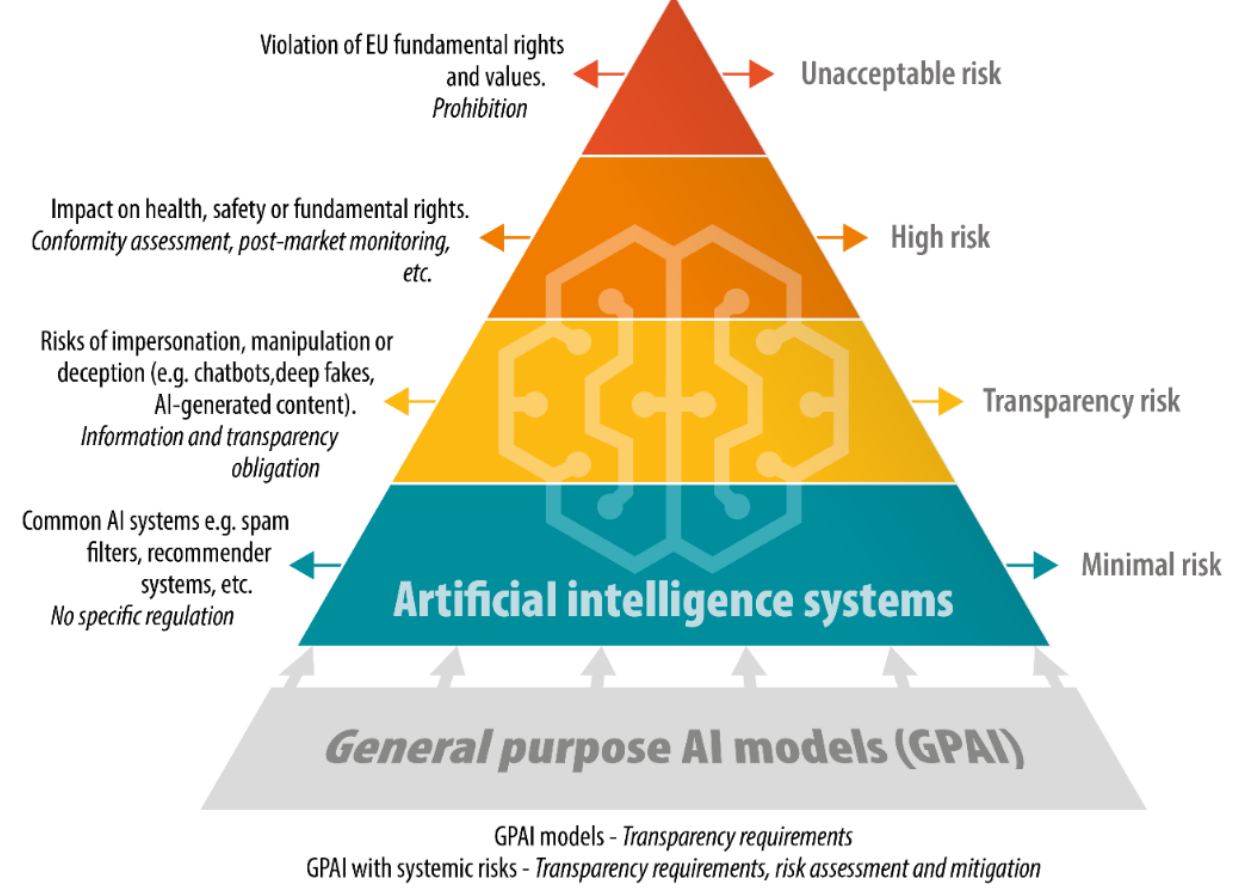
\includegraphics[width=.9\textwidth]{screen2.png}
\caption{pgAdmin Query tool}
\label{fig:querytool}
\end{figure}

When the pgAdmin application is initially launched, it will connect to the DBMS that is running on the local machine (''localhost'') with the username ''busi4720'' (its password is ''busi4720'') and will show an ''Object Explorer'' in the left part of the application. This allows navigation and exploration of the contents of this DBMS, as shown in Figure~\ref{fig:querytool}.

\begin{figure}
\centering
\includegraphics[width=.9\textwidth]{screen4.png}
\caption{DBeaver database tool}
\label{fig:dbeaver}
\end{figure}

Similarly, when the DBeaver application is first started, it will also conncect to the DBMS that is running on the local machine and will show a ''Database Navigator'' in the left part of the application window (Figure\ref{fig:dbeaver}. Navigate the contents of the DBMS to the ''busi4720'' database and the ''public'' schema.

\begin{figure}
\centering
\includegraphics[width=.9\textwidth]{screen3.png}
\caption{psql command line tool}
\label{fig:psql}
\end{figure}

The basic ''psql'' command line tool can be started by by typing \texttt{psql} into a terminal window. The course virtual machine is configured to provide automatic access to the ''busi4720'' database. The database connection can be confirmed by executing the \texttt{\textbackslash conninfo} command in psql. Use psql options to specify other connections using the template \texttt{psql -d dbname -h hostname -u username}. Figure~\ref{fig:psql} shows the psql command line tool in a terminal window.

\begin{tcolorbox}[colback=alert]
\noindent \emph{The examples and exercises in the remainder of this chapter refer to the ''busi4720'' database.}
\end{tcolorbox}

\section{Data Definition in SQL}

\begin{tcolorbox}[colback=code]
\paragraph*{Tip:} SQL commands are traditionally written in upper case letters and this is done here as well. However, SQL is not case sensitive, so that capitalization does not actuallly matter. Traditionally, an SQL command must end with a semicolon. This is done here as well, although some DBMS may no longer require this. 
\end{tcolorbox}

For this example, assume that your database will be used to store information about products. The CREATE TABLE data definition command in SQL\index{Data definition language!SQL} is used to create tables, their columns, and constraints. This first example creates a simple table with three columns to store product data.

\begin{tcolorbox}[colback=code]
Enter the SQL commands in the code block below.
\begin{itemize}
   \item In psql, press \colorbox{lightgray}{RETURN} to execute
   \item In DBeaver, press \colorbox{lightgray}{CTRL-RETURN} to execute
   \item In pgAdmin, press \colorbox{lightgray}{F5} to execute.
\end{itemize}
\end{tcolorbox}

\begin{samepage}
\begin{sqlcode}
CREATE TABLE products (
  pcode integer,
  name  varchar(100) NOT NULL,
  price float4,
  PRIMARY KEY (pcode) 
);
\end{sqlcode}
\end{samepage}

The table contains a column named ''pcode'' (to store the product code) that is of integer type, that is, it can contain whole numbers only. The table has a column called ''name'' of characters with a varying length and a maximum length of 100 characters to store product names. Additionally, a column NOT NULL constraint has been defined for this column, ensuring that a name always exists for a product. The table has a column named ''price'' that is of a single precision floating point type (4 bytes), that is, it can hold decimal point numbers to store product prices. The final line of the SQL command created a primary key constraint on the single column ''pcode'' to ensure that the product code must not be NULL and must be unique, ensuring that each row in the table represents a distinct product. Note that column ''price''may be NULL, that is, may not contain values, because no NOT NULL constraints have been specified. This may be useful for example when the price has not been decided on or will be calculated later.

The following SQL code block creates a table for suppliers. The table has a similar structure to the products table and similar NOT NULL and PRIMARY KEY constraints.

\begin{samepage}
\begin{sqlcode}
CREATE TABLE suppliers (
  scode integer,
  name  varchar(100) NOT NULL,
  city  varchar(100),
  PRIMARY KEY (scode) 
);
\end{sqlcode}
\end{samepage}

After creating tables with the data definition part of the SQL language, the data manipulation commands of SQL can be used to insert or update values in the tables. The following SQL code block inserts two rows into each of the tables that were just created. Enter the following SQL commands in the Query tool:

\begin{samepage}
\begin{sqlcode}
INSERT INTO products VALUES (1, 'Hex Bolt', 1.99);
INSERT INTO products VALUES (2, 'Round Bolt', 2.99);

INSERT INTO suppliers VALUES (1, 'Bolts Inc', 'HVGB');
INSERT INTO suppliers VALUES (2, 'Hardware Co', 'Cartwright');
\end{sqlcode}
\end{samepage}

The values for each row must be specified in the order in which the columns of the table are defined. For the ''products'' table this is first the product code, followed by the name, and finally the price. For the ''suppliers'' table, this is first the supplier code, then the name and then the city. There are many different variations on the basic INSERT statement; consult the official documentation using the links in the earlier footnote.

After inserting the values, a basic SELECT statement, which is the core querying command in SQL, checks that the data is actually in the tables. Run the commands in the following SQL code block one at a time to see each command's results:

\begin{samepage}
\begin{sqlcode}
SELECT * FROM products;
SELECT * FROM suppliers;
\end{sqlcode}
\end{samepage}

This is the simplest form of a SELECT statement, the asterisk (''*'') instructs SQL to retrieve all columns. Later examples will illustrate ways to retrieve only some columns, and many other variants on the SELECT statement.

The two tables allow capturing information about products and information about suppliers, but they do not allow capturing which supplier supplies which product. In order to do this, the two tables need to be related by a foreign key relationship. 

For the following example, assume that suppliers can supply many products, but a product may be supplied by only one supplier (or no supplier at all). This is called a \emph{one-to-many relationship}. The following SQL code block alters the tables, retaining the existing data, and then updates the information in the new ''supplier'' column for the ''products'' table:

\begin{samepage}
\begin{sqlcode}
ALTER TABLE products ADD COLUMN supplier integer;
ALTER TABLE products ADD FOREIGN KEY (supplier) REFERENCES suppliers;

UPDATE products SET supplier = 1 WHERE pcode = 1;
UPDATE products SET supplier = 1 WHERE pcode = 2;
\end{sqlcode}
\end{samepage}

The first SQL statement above adds a new column to the existing products table in which to record the supplier of the product. The second line creates a foreign key reference from the supplier column in the products table to the primary key of the suppliers table; the primary is the ''scode'' column (see SQL code above). This ensures that only those suppliers can be recorded in the products table that actually exist in the suppliers table. 

The third and fourth line update the data in the products table and set the value of the supplier column for different products. The two products have the same supplier which reflects the assumption that a supplier may supply multiple products. On the other hand, only one supplier can be recorded for each product, and this too reflects the above assumption. This expresses the \emph{one-to-many relationship}. Moreover, the value of the supplier column in the products table may be NULL. In fact, after altering the table to add this column, all its values were NULL. A NULL value reflects the fact that a product has no supplier.

As an alternative to altering the existing products table, drop the products table to delete it and re-create it. Then insert some values. The following SQL code block uses the DROP TABLE command of SQL to delete the products table and all its contents.

\begin{samepage}
\begin{sqlcode}
DROP TABLE products;

CREATE TABLE products (
  pcode    integer,
  name     varchar(100),
  price    float4,
  supplier integer,
  PRIMARY KEY (pcode),
  FOREIGN KEY (supplier) REFERENCES suppliers 
);
  
INSERT INTO products VALUES(1, 'Hex Bolt', 1.99, 1);
INSERT INTO products VALUES(2, 'Round Bolt', 2.99, 1);
INSERT INTO products VALUES(3, 'Square Bolt', 3.99, NULL);
\end{sqlcode}
\end{samepage}

The above SQL code achieves the same as altering the table but in the process deletes all data in the products table. When possible, it is therefore preferable to use multiple ALTER TABLE statements instead of DROP and CREATE statements. 

Note the following important points about the tables so far:
\begin{itemize}
  \item There are products that have no supplier (the ''square bolt'')
  \item There are suppliers that supply many products (supplier 1)
  \item There are suppliers that do not supply products (supplier 2)
\end{itemize}

In the products table as altered or re-created to this point, it is possible that a product has no supplier. However, in some applications it may be necessary to enforce that it is mandatory for products to have a supplier. This is done by adding a NOT NULL constraint, either by altering the table again, as in the following SQL code block, or by re-creating it with the appropriate constraint added.

\begin{sqlcode}
ALTER TABLE products ALTER COLUMN supplier SET NOT NULL;
\end{sqlcode}

Adding constraints can only be done when the constraint is already satisfied. This means that in this example, none of the values of the supplier columns can be NULL when adding the constraint. If a new constraint is violated, the DBMS will show an error and the constraint will not be added.

When re-creating the table, the NOT NULL column constraint can be defined in the CREATE TABLE statement:

\begin{samepage}
\begin{sqlcode}
DROP TABLE IF EXISTS products;

CREATE TABLE products (
  pcode    integer,
  name     varchar(100),
  price    float4,
  supplier integer NOT NULL,
  PRIMARY KEY (pcode),
  FOREIGN KEY (supplier) REFERENCES suppliers 
);
\end{sqlcode}
\end{samepage}

So far, the assumption was that each product can has one supplier. However, in many settings, products have multiple suppliers, and suppliers supply multiple products, that is, there is a \emph{many-to-many relationship} between the two. Expressing many-to-many relationships requires a third table that explicitly represents the relationship, here the ''supplies'' relatinship between products and suppliers. The following SQL code first removes the existing tables, then re-creates tables to express a many-to-many relationship instead.

\begin{samepage}
\begin{sqlcode}
DROP TABLE IF EXISTS products;
DROP TABLE IF EXISTS suppliers;

CREATE TABLE products (
  pcode integer,
  name  varchar(100),
  PRIMARY KEY (pcode) );

CREATE TABLE suppliers (
  scode integer,
  name  varchar(100),
  city  varchar(100),
  PRIMARY KEY (scode) );
  
CREATE TABLE supplies (
  scode  integer NOT NULL,
  pcode  integer NOT NULL,
  price  float4 NOT NULL,
  PRIMARY KEY (scode, pcode),
  FOREIGN KEY (scode) REFERENCES suppliers,
  FOREIGN KEY (pcode) REFERENCES products );
\end{sqlcode}
\end{samepage}

Note that the tables must be dropped in the right order: ''products'' first, then ''suppliers'' because the products depend on the suppliers due to the foreign key constraint\footnote{Use the CASCADE keyword to drop dependent tables automatically but use with care.}. The IF EXISTS part is a safeguard to prevent an error if the table does not exist when attempting to drop it.

The primary key of the supplies table is a \emph{compound key}\index{Compound key}, that is, it consists of a combination of columns. The supplies table is related by two FOREIGN KEY constraints both to the products and suppliers table so that only products and suppliers that already exist can be recorded here (and thereby related to each other). The price column is no longer in the products table, but has been moved to the supplies table, because each supplier may supply a product at a different price. The following example data shows this:

\begin{samepage}
\begin{sqlcode}
INSERT INTO products VALUES (1, 'Hex Bolt');
INSERT INTO products VALUES (2, 'Round Bolt');

INSERT INTO suppliers VALUES (1, 'Bolts Inc', 'HVGB');
INSERT INTO suppliers VALUES (2, 'Hardware Co', 'Cartwright');

INSERT INTO supplies VALUES(1, 1, 1.99);
INSERT INTO supplies VALUES(1, 2, 2.49);
INSERT INTO supplies VALUES(2, 1, 2.99);
INSERT INTO supplies VALUES(2, 2, 1.79);
\end{sqlcode}
\end{samepage}

\noindent To clean up after these exercises, drop all tables if they are no longer required:

\begin{samepage}
\begin{sqlcode}
DROP TABLE supplies;
DROP TABLE products;
DROP TABLE suppliers;
\end{sqlcode}
\end{samepage}

\paragraph*{Summary} In summary, a \emph{one-to-many relationships} requires a foreign key from the ''many'' table that references the ''one'' table and its primary key. In the first example above, a supplier supplies many products but a product has one supplier (or none, depending on whether a NOT NULL constraint has been specified). In contrast, a \emph{many-to-many relationship} requires a table that explicitly represents the relationship. Foreign keys from this table reference the participating, original, ''main'' tables and their primary keys. In the second example above, a supplier supplies many products and a product can be supplied by many suppliers. 

In fact, this type of relationship can be extended in a straightforward way to three or more tables. For example, a supplier supplies many products from many warehouses, a product may be supplied by many suppliers from many warehouses, and a warehouse may contain many products from many suppliers. 

\begin{tcolorbox}[colback=code]
\subsubsection*{Hands-On Exercise}
\begin{enumerate}
  \item Consider the following information:
	\begin{itemize}
	  \item A book has an ISBN number and a title. 
	  \item An author has a name and an address. 
	  \item An author can write many books, and a book can be written by multiple authors. A book is written in a certain year.
	\end{itemize}
  \item Write the CREATE TABLE statements with the necessary FOREIGN KEY statements, and execute them on PostgreSQL
  \begin{itemize}
    \item Use appropriate datatypes for the columns
    \item Create an appropriate PRIMARY KEY for all tables
  \end{itemize}
  \item Use INSERT statements to create some example data.
  \item Use SELECT statements to ensure your data exists.
\end{enumerate}
\end{tcolorbox}

\section{SQL Queries}

\subsection*{Basic Queries with the SELECT Statement}

The SELECT statement in SQL is used to query and retrieve data from one or more tables in a database. The basic structure of a SELECT statement allows specification of which columns of data you want to retrieve and from which tables. A SELECT statement has multiple clauses or parts that are used to specific different characteristics of the information to retrieve:

\begin{samepage}
\begin{itemize}
 \item \texttt{SELECT}: Which columns to query (use the asterisk ''\texttt{*}'' to select all).
 \item \texttt{FROM}: Which tables to query from.
 \item \texttt{JOIN}: How to combine data from multiple tables based on related columns.
 \item \texttt{WHERE}: Conditions on field values used to filter the retrieved records.
 \item \texttt{GROUP BY}: Groups within which to aggregate data using an aggregate function such as \texttt{sum()}, \texttt{count()}, or \texttt{max()}.
 \item \texttt{HAVING}: Conditions on group aggregate values. Similar to WHERE but for aggregates within each group.
 \item \texttt{ORDER BY}: How to sort the resulting records in either ascending or descending order.
 \item \texttt{LIMIT}: Limit on how many results to return.
\end{itemize}
\end{samepage}

To demonstrate the basic use of SQL queries to retrieve information from a relational database, it is best to begin with a simple example, that of the 1:Many relationship between products and suppliers set up earlier. The following SQL commands (re-)create this example with a few more rows of data in the products table:

\begin{samepage}
\begin{sqlcode}
-- Drop tables if they exist
DROP TABLE IF EXISTS products;
DROP TABLE IF EXISTS suppliers;

-- Set up tables with 1:Many relationship:
CREATE TABLE suppliers (
scode integer,
name varchar(100),
city varchar(100),
PRIMARY KEY (scode) );

CREATE TABLE products (
pcode	integer,
name	varchar(100),
price	float4,
scode   integer,
PRIMARY KEY (pcode),
FOREIGN KEY (scode) REFERENCES suppliers );
\end{sqlcode}
\end{samepage}

\begin{samepage}
\begin{sqlcode}
-- Insert some data:
INSERT INTO SUPPLIERS VALUES (1, 'Bolts Inc', 'HVGB');
INSERT INTO SUPPLIERS VALUES (2, 'Hardware Co', 'Cartwright');

INSERT INTO products VALUES(1, 'Hex Bolt A', 1.99, 1);
INSERT INTO products VALUES(2, 'Round Bolt 1', 2.99, 1);
INSERT INTO products VALUES(3, 'Square Bolt B', 3.99, 1);
INSERT INTO products VALUES(4, 'Hex Bolt B', 2.99, 1);
INSERT INTO products VALUES(5, 'Round Bolt 2', 1.99, 2);
INSERT INTO products VALUES(6, 'Square Bolt 7', 3.49, 2);
\end{sqlcode}
\end{samepage}

With this data, the simplest SQL query contains only the SELECT and the FROM clauses to retrieve a set of columns from a single table. The following SQL code uses the asterisk (''\texttt{*}'') to select all columns and returns all rows from the products table:

\begin{sqlcode}
SELECT * FROM products;
\end{sqlcode}

The WHERE clause filters the selected rows. The next example returns only products for supplier 1, that is, those rows in the products table where ''scode=1''. Multiple conditions can be surrounded in parentheses and combined with the keywords AND and OR.

\begin{sqlcode}
SELECT * FROM products WHERE scode = 1;
\end{sqlcode}

The following SQL code selects only a few named columns from the products table and also filters the retrieved rows by price:

\begin{sqlcode}
SELECT name, supplier FROM products WHERE price < 3;
\end{sqlcode}

The ORDER BY clause is used to order the result, possibly by using multiple columns and with specified ascending or descending direction. The following SQL code block selects all columns and returns all rows from the products table ordered first ascending by price, and then, when the price is the same, descending by name:

\begin{sqlcode}
SELECT * FROM products ORDER BY price ASC, name DESC;
\end{sqlcode}

The LIMIT clause can be used to limit the number of returned rows. This is often useful in combination with the ORDER BY clause to select the largest or smallest values. The following example demonstrates this by retrieving the name of the cheapest three products from the products table:

\begin{sqlcode}
SELECT name FROM products ORDER BY price ASC LIMIT 3;
\end{sqlcode}

The JOIN clause combines information from two or more tables. This is done by specifying either a common column, or an explicit join condition if the corresponding column names in the two tables are different. The following SQL code shows an example of retrieving all columns from the products table and their corresponding rows from the suppliers table using an INNER JOIN clause USING the common column ''scode'':

\begin{sqlcode}
SELECT * FROM products INNER JOIN suppliers USING (scode);
\end{sqlcode}

If multiple common columns are needed to find corresponding rows, they can be specified in parentheses simply be expanding the above example of the USING clause.

The following two SQL expressions are essentially equivalent to the one above and to each other. Instead of the USING clause for common columns, the first expression explicitly specifies the join condition with the ON clause, while the second expression completely omits the JOIN clause and instead specifies both tables in the FROM clause and uses a condition in a WHERE clause to select corresponding rows in the two tables:

\begin{samepage}
\begin{sqlcode}
-- (Almost) Equivalent:
SELECT * FROM products 
    INNER JOIN suppliers ON products.scode=suppliers.scode;

SELECT * FROM products, suppliers 
    WHERE products.scode=suppliers.scode;
\end{sqlcode}
\end{samepage}

In the above JOIN examples, both the products and suppliers table contain a column ''name''. It is often useful to rename columns for clarity. The following example shows how this can be done using the AS keyword. It also demonstrates how the ambiguity of columns with the same name in different tables can be resolved by using the form ''table.column'' to select columns:

\begin{samepage}
\begin{sqlcode}
-- Rename columns for clarity:
SELECT products.name AS "Product", 
       price AS "Price", 
       suppliers.name AS "Supplier", 
       city AS "Location"
    FROM products INNER JOIN suppliers USING (scode);
\end{sqlcode}
\end{samepage}

The previous two examples used the ''INNER JOIN'', the most commonly used type of join between two tables. Table~\ref{tab:sqljoins} shows a list of other possible join types. 

The INNER JOIN selects only those rows that have a corresponding row or rows in the other table, and vice versa. The LEFT OUTER join selects all rows from table T1, even those that do not have a corresponding row in table T2. For the missing corresponding rows, it simply returns NULL values. The RIGHT OUTER join does the same thing but from the perspective of table T2. That is, it returns all rows of T2, but for those rows that do not have a corresponding entry in table T1, it returns NULL values. The FULL OUTER join is a combination of the LEFT OUTER and RIGHT OUTER joins.

\begin{table}
\centering

\renewcommand{\arraystretch}{1.5}
\small
\begin{tabularx}{.8\textwidth}{l|X} \hline
INNER & Selects only rows from T1 that have corresponding row in T2 and vice versa. \\
LEFT OUTER & Selects all rows from T1, if T2 does not have a corresponding row, NULL values are inserted. \\
RIGHT OUTER & Select all rows from T2, if T1 does not have a corresponding row, NULL values are inserted. \\
FULL OUTER & Selects all rows from T1, T2. If the other table is missing corresponding row, NULL values are inserted. \\ \hline
\end{tabularx}

\caption{Types of Joins between two tables T1 and T2 in SQL}
\label{tab:sqljoins}
\end{table}

The GROUP BY clause of an SQL query is used in combination with aggregate functions for grouping information and calculating aggregate values. The easiest aggregation is to simply count the number of rows or entries for each group using the ''count(.)'' function, shown in the first example that selects the number of products for each supplier, that is, the count of rows in table products grouped by supplier code:

\begin{samepage}
\begin{sqlcode}
-- Select the number of products for each supplier
SELECT scode, count(*) from products GROUP BY scode;
\end{sqlcode}
\end{samepage}

To also include the names of the suppliers requires joining the suppliers table, as shown below:
\begin{samepage}
\begin{sqlcode}
-- Add the name of suppliers by joining suppliers table
SELECT suppliers.name, count(*)
    FROM suppliers INNER JOIN products USING (scode)
    GROUP BY scode;
\end{sqlcode}
\end{samepage}

The SQL code below illustrates another aggregate function, the average (''AVG'') and also shows that the aggregates can be used in the ORDER BY clause. The query returns the mean price of products for each suppliers, ordered descending by mean price:

\begin{samepage}
\begin{sqlcode}
-- Mean price of products for each supplier, ordered descending
SELECT suppliers.name, AVG(price)
    FROM suppliers INNER JOIN products USING (scode)
    GROUP BY scode
    ORDER BY AVG(price) DESC;
\end{sqlcode}
\end{samepage}

Finally, the HAVING clause is a filter clause like the WHERE clause, but instead of filtering the rows in a table, it filters the groups in a GROUP BY clause. The following SQL query returns only suppliers for which the average price of their products is less than 2.8:

\begin{samepage}
\begin{sqlcode}
-- Find only suppliers for which average price less than 2.80:
SELECT suppliers.name, AVG(price)
    FROM suppliers INNER JOIN products USING (scode)
    GROUP BY scode
    HAVING AVG(price) < 2.8;
\end{sqlcode}
\end{samepage}

Besides COUNT() and AVG() functions, SQL provides other aggregate functions, shown in Table~\ref{tab:sqlaggregates}. However, many of these are specific to various relational database management systems, like PostgreSQL. 

\begin{table}
\centering

\renewcommand{\arraystretch}{1.5}
Standard SQL: \\

\small
\begin{tabular}{l|l|l|l|l} \hline
\
MIN() & MAX() & COUNT() & SUM() & AVG() \\ \hline
\end{tabular}

\normalsize

\vspace{\baselineskip}
PostgreSQL (excerpt):\\

\small
\begin{tabular}{l|l|l} \hline
CORR() & STDDEV() & VARIANCE() \\
MODE() & PERCENTILE() & REGR\_SLOPE() \\
REGR\_R2() & RANK() & DENSE\_RANK() \\ \hline
\end{tabular}

\caption{Frequently Used Aggregation Functions}
\label{tab:sqlaggregates}
\end{table}

\noindent To clean up after these exercises, drop all tables if they are no longer required:

\begin{samepage}
\begin{sqlcode}
DROP TABLE products;
DROP TABLE suppliers;
\end{sqlcode}
\end{samepage}

\subsection*{Relational Diagrams}

The previous section has presented the basics of the relational database model, focusing on how tables are related by foreign key relationships. Tables and their relationships are often graphically shown in a \emph{relational diagram}\index{Relational diagram}. Such diagrams are often called ''\emph{ER Diagrams}\footnote{Technically, the two are not quite the same.}''\index{ER diagram|see{Entity-relationship diagram}} or ''Entity-Relationship Diagrams''\index{Entity-relationship diagram}. A graphical representation of the database structure is useful for understanding the data and for writing queries to extract data from the table or tables of the database. 

In many software tools, including in pgAdmin, the database developer can use relational diagrams to create tables, instead of writing CREATE TABLE statements. In the reverse, relational diagrams can also be automatically created from an existing database and its tables. 

\begin{tcolorbox}[colback=code]
\subsubsection*{Hands-On Exercise}

In the pgAdmin Object Explorer, right-click on the ''busi4720'' database, then select ''ERD for Database'' to create a relational diagram. \\

In the DBeaver Database Navigator, select the ''busi4720'' database, then right-click on its ''public'' schema and select ''View Diagram'' to create the diagram.
\end{tcolorbox}

\noindent The resulting diagram will look similar to the one in Figure~\ref{fig:pagila}. (If you did not clean up the tables you created in the above SQL exercises, these will be present in the diagram as well).

\begin{figure}
\centering

\includegraphics[width=.95\textwidth]{pagila2dbeaver.png}
\caption{Relational diagram of the Pagila demo database}
\label{fig:pagila}
\end{figure}


\subsection*{The Pagila Database}

The diagram shows the structure of the \emph{Pagila} database\footnote{\url{https://github.com/devrimgunduz/pagila}, \\
\url{https://github.com/devrimgunduz/pagila/blob/master/LICENSE.txt}}, a demonstration database originally developed for teaching and development of the MySQL RDBMS under the name Sakila\footnote{\url{https://dev.mysql.com/doc/sakila/en/}, \\
\url{https://dev.mysql.com/doc/sakila/en/sakila-license.html}}. Pagila is designed as a sample database to illustrate database concepts and is based on a fictional DVD rental store. It consists of multiple tables for film and actor information, customer data, store inventory, and rental transactions. Here is an overview of the key tables in the Pagila database:

\begin{itemize}
  \item \emph{actor}: Stores details about actors, including their first and last names.
  \item \emph{film}: Contains information about movies, such as title, release year, language, rental duration, rental rate, length, replacement cost, rating, and special features.
  \item \emph{film\_actor}: A junction table that establishes a many-to-many relationship between the films and actors. It links each film to its actors.
  \item \emph{category}: Lists different genres or categories of films.
  \item \emph{film\_category}: Another junction table that connects films to their respective categories.
  \item \emph{language}: Stores languages in which the films are available.
  \item \emph{customer}: Contains customer information, including names, email addresses, addresses, and store ID where they are registered.
  \item \emph{address}: Holds address details, including city, postal code, phone number, and other address components.
  \item \emph{city}: Contains information about cities, linked to the addresses.
  \item \emph{country}: Stores country information, which is linked to cities.
  \item \emph{store}: Includes data about the DVD rental stores, such as the store's address and the staff.
  \item \emph{inventory}: Contains information about the store's inventory, including which film copies are available at which store.
  \item \emph{rental}: Records details about rental transactions, including rental and return dates, inventory, and customer information.
  \item \emph{payment}: Tracks payments made by customers for rentals, including amount and payment date.
  \item \emph{staff}: Contains information about the store staff, including their names, email addresses, and the store they work in.
\end{itemize}

Each table is designed with primary keys for unique identification and foreign keys to establish relationships with other tables. This structure allows for complex queries across multiple tables, facilitating a wide range of analyses, from inventory management to customer behavior tracking. The Pagila database is a good example of a real-world database schema and offers a good data set for practicing SQL queries.

\subsection*{Advanced SQL Query Examples}

The following examples show queries for the Pagila database to illustrate different features of the SELECT statement. Instead of describing every option in detail, to understand SQL it is useful to execute the queries and learn by modifying the queries and observing changes in the results. 

\paragraph{Example:} Find all actors and the films they appeared in, ordered by film category and year, for those films that are rated PG

\begin{samepage}
\begin{sqlcode}
SELECT concat(left(actor.first_name, 1), '. ', 
           actor.last_name) AS Actor, 
       category.name AS Category, 
       film.title, 
       film.release_year
  FROM film_actor
  INNER JOIN actor USING (actor_id)
  INNER JOIN film USING (film_id)
  INNER JOIN film_category USING (film_id)
  INNER JOIN category USING (category_id)
  WHERE film.rating = 'PG'
  ORDER BY actor.last_name, 
           actor.first_name, 
           category.name ASC, 
           film.release_year DESC, 
           film.title ASC;
\end{sqlcode}
\end{samepage}

Running this query will retrieve 1143 records from the Pagila database. 

The \texttt{SELECT} clause specifies only a few columns to retrieve. Note that column names are prefixed by the table name, as in ''actor.first\_name'' to make them unambiguous when multiple tables contain columns with the same name. Some columns are also given \emph{aliases} using the keyword \texttt{AS}. This is useful to give the results more meaningful and shorter names. The first item to be selected is the result of a \emph{function}: The \texttt{concat()} function concatenates text, and the \texttt{left()} function extracts the left part of some text. Refer to the PostgreSQL documention linked to in the footnote above for a complete reference to available functions. 

The \texttt{FROM} clause specifies a single table ''film\_actor'' to which other tables are joined using the \texttt{INNER JOIN} keyword. The \texttt{JOIN} clause specifies the common join column with the \texttt{USING} keyword. The join columns typically correspond to the columns related by a foreign key relationship. In the Pagila database, foreign keys are always single columns, as are primary keys. However, one can imagine that combinations of two or more columns serve as primary keys and as foreign keys. Then, multiple columns are specified in the USING clause.

An \texttt{INNER JOIN}\index{Join (in SQL)} is a type of join that matches records from two tables if they both have the same value in their join columns, and only if they both have non-null values in their join columns. In contrast, a \texttt{LEFT OUTER JOIN} would also include records from the left table that have a NULL value in their join columns, a \texttt{RIGHT OUTER JOIN} would also includes records from the right table that have a NULL value in their join columns, and a \texttt{FULL OUT JOIN} is the combination of a \texttt{LEFT OUTER JOIN} and a \texttt{RIGHT OUTER JOIN}.

Compare the \texttt{FROM} and \texttt{JOIN} clauses to the relational diagram in Figure~\ref{fig:pagila} and notice how it allows you to ''navigate'' from one table to another table along the foreign key relationships that link each table.

The \texttt{WHERE} clause in the above example selects those films whose rating is equal to the text ''PG''. Multiple logical conditions can be combined with the \texttt{AND}, \texttt{OR}, \texttt{NOT} keywords and parentheses.

The \texttt{ORDER BY} clause specifies the ordering of the results. In this case, ordering is first done by actor last name. When actors have the same last name, ordering is done by first name. Within the same last and first names, ordering is done by category name, in ascending order, as indicated by the \texttt{ASC} keyword (The default ordering is always ascending, but it is sometimes useful to explicitly indicate this). Next, results are sorted by film release year in descending order, then again by film title in ascending order.

The \texttt{JOIN \ldots USING} clause assumes that the columns have the same name in both tables. When this is not the case, this short form is not available and joins must be specified manually. Recall that the join ensures that the join columns in both tables have the same value, which can also be specified in a \texttt{WHERE} clause as a set of conditions. The following query is equivalent to the previous one, but without the \texttt{JOIN} clauses:

\begin{samepage}
\begin{sqlcode}
SELECT concat(left(actor.first_name, 1), '. ', 
           actor.last_name) AS Actor, 
       category.name AS Category, 
       film.title, 
       film.release_year
  FROM film_actor, film, actor, film_category, category
  WHERE actor.actor_id = film_actor.actor_id AND
        film.film_id = film_actor.film_id AND
        film_category.film_id = film.film_id AND
        category.category_id = film_category.category_id AND
        film.rating = 'PG'
  ORDER BY actor.last_name, 
           actor.first_name, 
           category.name ASC, 
           film.release_year DESC, 
           film.title ASC;
\end{sqlcode}
\end{samepage}

When writing the query without \texttt{JOIN} keywords, the required tables must all be included in the \texttt{FROM} clause; it does not matter in which order they are listed there.

\paragraph{Example:} Find the most popular actors in the rentals in each city

\begin{samepage}
\begin{sqlcode}
SELECT city.city, 
       concat(actor.first_name, '. ', actor.last_name) AS actor_name,
       count(rental.rental_id) AS Number_Rentals
  FROM rental
  INNER JOIN inventory USING (inventory_id)
  INNER JOIN store USING (store_id)
  INNER JOIN address USING (address_id)
  INNER JOIN city USING (city_id)
  INNER JOIN film USING (film_id)
  INNER JOIN film_actor USING (film_id)
  INNER JOIN actor USING (actor_id)
  GROUP BY city.city, actor.actor_id
  HAVING count(rental.rental_id) >= 300
  ORDER BY city ASC, 
           Number_Rentals DESC, 
           actor_name ASC;
\end{sqlcode}
\end{samepage}

Running this query will retrieve 22 records from the Pagila database.

This query uses the \texttt{GROUP BY} clause to group data. First, data is grouped by the city name, then, within each city, data is grouped by actor identification. Grouping allows, and in fact requires, the use of \emph{aggregate functions}. This query uses the \texttt{count()} function to count the number of rentals in each group, that is, for each combination of city and actor. This query also includes a \texttt{HAVING} clause to return only those groups for which the count of rentals is greater than or equal to 300. 

\paragraph*{Example:} Find the customers who spent the most, with their phone numbers and cities, the cities their store is in, and the number of rentals with the highest total rental payments for each film category, grouped by city of the rental store.

\begin{sqlcode}
SELECT category.name AS category_name, 
       store_city.city AS store_city,
       customer.customer_id, 
       concat(customer.first_name, ' ', 
           customer.last_name) AS customer_name,
       cust_city.city AS customer_city,
       cust_address.phone AS customer_phone,
       count(rental.rental_id) AS num_rentals,
       sum(amount) AS total_amount
 FROM city AS cust_city, city AS store_city, 
      address AS cust_address, address AS store_address, 
      store, rental
 INNER JOIN payment USING (customer_id)
 INNER JOIN customer USING (customer_id)
 INNER JOIN inventory USING (inventory_id)
 INNER JOIN film USING (film_id)
 INNER JOIN film_category USING (film_id)
 INNER JOIN category USING (category_id)
 WHERE store.store_id = inventory.store_id
   AND store_address.address_id = store.address_id
   AND store_city.city_id = store_address.city_id
   AND cust_address.address_id = customer.address_id
   AND cust_city.city_id = cust_address.city_id
 GROUP BY category.name, customer.customer_id, 
         cust_address.address_id, cust_city.city, store_city.city
 HAVING sum(amount) IN (
  SELECT sum(amount) AS maxamount
   FROM store, address, city AS inner_city, rental
   INNER JOIN payment USING (customer_id)
   INNER JOIN customer USING (customer_id)
   INNER JOIN inventory USING (inventory_id)
   INNER JOIN film USING (film_id)
   INNER JOIN film_category USING (film_id)
   INNER JOIN category AS inner_category USING (category_id)
   WHERE inner_category.name = category.name AND
         inner_city.city = store_city.city AND
         store.store_id = inventory.store_id AND
         address.address_id = store.address_id AND
         inner_city.city_id = address.city_id
   GROUP BY inner_category.name, inner_city.city, 
            customer.customer_id
   ORDER BY inner_category.name ASC, inner_city.city, 
            maxamount DESC
   LIMIT 1 )
 ORDER BY category.name ASC, store_city ASC;
\end{sqlcode}

This query will return 33 records from the Pagila database.

This complex query is actually two queries as it includes a \emph{subquery}\index{Subquery} within the \texttt{HAVING} clause! Starting in the \texttt{FROM} clause, notice that some tables are included twice in this query, under different \emph{aliases} or names, using the \texttt{AS} keyword. This is because the query retrieves the city that the customers live in, as well as the city that the store is located in. As cities are linked to addresses, the address table is also included twice. 

Some joins are done using the \texttt{JOIN} keyword on common columns, while joining the address and city tables is done in the \texttt{WHERE} clause because the column names ''city\_id'' and ''address\_id'' are ambiguous as the tables are included multiple times. 

The \texttt{GROUP BY} keyword groups the results by category, customer, address, customer city, and store city. This is necessary to be able to the select the customer city and address: Only columns that are groupbed by can be retrieved or selected and aggregated, for example by using the \texttt{sum()} function used in this query. 

As the query seeks to retrieve the maximum amount spent, the \texttt{HAVING} clause is used to select just this maximum by ensuring that the sum of payment amounts is equal to the result of the subquery. This subquery is very similar to the ''outer'' query, but returns only the sum of payment amounts, ordered by this amount in descending order and limited to the first result. That is, the subquery returns the maximum sum of payment amounts. The subquery is linked to the outer query by two conditions in its \texttt{WHERE} clause: \texttt{inner\_category.name = category.name} and \texttt{inner\_city.city == store\_city.city}. These two conditions ensure that the maximum sum of payments computed in the subquery is done for the same grouping that the outer query is considering.

Because of the subquery, running this query is expensive in terms of computing time.

\paragraph*{Example:}
Get the total rental revenue and number of rentals for each store by month


\begin{samepage}
\begin{sqlcode}
SELECT city.city, 
       extract(year from payment_date) AS year, 
       extract(month from payment_date) AS month, 
       sum(amount) as dollars, 
       count(rental.rental_id) as rentals
FROM payment, rental, inventory, store, address, city
WHERE payment.rental_id = rental.rental_id AND
      rental.inventory_id = inventory.inventory_id AND
      inventory.store_id = store.store_id AND
      store.address_id = address.address_id AND
      address.city_id = city.city_id
GROUP BY city.city, 
         extract(year from payment_date), 
         extract(month from payment_date)
ORDER BY city.city, 
         extract(year from payment_date), 
         extract(month from payment_date);
\end{sqlcode}
\end{samepage}

Running this query will return 14 results.

This query shows the use of a date function in PostgreSQL. The \texttt{extract()} function can extract part of a date. In the example, it is used to extract the year and the month. Both are also used in the \texttt{GROUP BY} and in the \texttt{ORDER BY} clause. 

\paragraph*{Example:} Get the top 5 and the bottom 5 grossing customers by year


\begin{samepage}
\begin{sqlcode}
( SELECT concat(customer.first_name, ' ', 
                customer.last_name) AS customer_name,
       extract(year from payment_date) AS year, 
       sum(amount) as dollars,
       'Top-5' as note
FROM payment, customer
WHERE payment.customer_id = customer.customer_id
GROUP BY extract(year from payment_date),
         customer.customer_id
ORDER BY dollars desc
LIMIT 5
) UNION (
SELECT concat(customer.first_name, ' ', 
              customer.last_name) AS customer_name,
       extract(year from payment_date) AS year, 
       sum(amount) as dollars,
       'Bottom-5' as note
FROM payment, customer
WHERE payment.customer_id = customer.customer_id
GROUP BY extract(year from payment_date),
         customer.customer_id
ORDER BY dollars asc
LIMIT 5 ) ORDER BY dollars DESC;
\end{sqlcode}
\end{samepage}

This query combines the results of two simple queries with the UNION keyword. Both queries must return the same columns in order to be combined in this way. Because the results are mathematically sets, they are not intrinsically ordered; this is why the set that results from the UNION operation is ordered again.

\emph{Set operations} can be used to combine results from multiple queries. These are specified by the \texttt{UNION}, \texttt{INTERSECT}, and \texttt{EXCEPT} keywords and do exactly as their name indicates: They return the union, the intersection, or the complement of two result sets. The inputs to each operation sets must have the same set of columns.

PostgreSQL can easily import and export data for further analysis. The pgAdmin application can export query results to CSV files (there is a button in the query toolbar). Alternatively, one can use the \emph{COPY} command as in the following example.

\begin{samepage}
\begin{sqlcode}
COPY (SELECT * FROM customer) 
  TO '/tmp/filename.csv' 
  WITH (FORMAT CSV, HEADER);
\end{sqlcode}
\end{samepage}

Similarly, PostgreSQL can easily import data from CSV files using the copy command:

\begin{samepage}
\begin{sqlcode}
COPY customer 
  FROM '/tmp/filename.csv' 
  WITH (FORMAT CSV, HEADER);
\end{sqlcode}
\end{samepage}

Addtionally, PostgreSQL can import and export JSON files; see the documentation for details.

\begin{tcolorbox}[colback=code]
\subsubsection*{Hands-On Exercise}
\begin{enumerate}
  \item Find the names and the rental numbers of the top 5 customers who rented the most films
  \begin{itemize}
    \item \textbf{Tip}: Join tables ''rental'', ''customer'', use the ''count()'' function
  \end{itemize}
  \item Calculate the rental revenue per customer. Who are the top 5? Bottom 5?
  \begin{itemize}
    \item \textbf{Tip}: Join tables ''rental'', ''customer'', ''payment'', use the ''sum()'' function
  \end{itemize}
  \item Calculate the average rental revenue per customer for each store
  \begin{itemize}
    \item \textbf{Tip}: Join tables ''rental'', ''customer'', ''payment'', ''inventory'', use the ''avg()'' function
  \end{itemize}
  \item Calculate the rental counts for each country of customer. Are there countries with no rentals?
  \begin{itemize}
    \item \textbf{Tip}: Join tables ''rental'', ''customer'', ''address'', ''city'', ''country'', use the ''count()'' function
  \end{itemize}
  \item Find all films with a single actor
  \begin{itemize}
    \item \textbf{Tip}: Join tables ''film'', ''film\_actor'', use the ''count()'' function in a HAVING clause
  \end{itemize}
  \item Create tables to represent a part-of hiearchy. For example, a product may be a part of another product, and prodcuts may have multiple parts.
  \begin{itemize}
    \item \textbf{Tip}: You need only one table
  \end{itemize}
\end{enumerate}
\end{tcolorbox}

\section{Review Questions}

\begin{enumerate}[nosep]
	\item What is a relational database, and who developed the relational model?
	\item Explain the role of primary keys and foreign keys in relational databases.
	\item What is SQL and what are its main purposes?
	\item List and describe at least four data types commonly used in SQL.
	\item Explain the difference between the \texttt{varchar} and \texttt{text} data types in PostgreSQL.
	\item What are the ACID properties in relational databases and what is their purpose?
	\item Define and give an example of each of the following constraints:
	\begin{enumerate}[label=\Alph*.]
		\item NOT NULL
		\item UNIQUE
		\item PRIMARY KEY
		\item FOREIGN KEY
		\item CHECK
	\end{enumerate}
	\item How do relational databases handle relationships between tables? Give examples.
	\item What are some of the challenges relational databases faced with the advent of Big Data?
    \item What is PostgreSQL and what type of system is it?
    \item What is the purpose of the ``psql'' and ``pgAdmin'' tools in the context of PostgreSQL?
    \item When connecting to a DBMS running on your own computer, what hostname should you use?
    \item Define a ``schema'' in the context of a PostgreSQL database. What is the default schema in PostgreSQL?
\end{enumerate}

    
\section{Additional SQL Exercises}

\textbf{Database Schema:} 
\begin{itemize}
    \item \textbf{Table:} Employees
    \item \textbf{Columns:} EmployeeID, FirstName, LastName, Role, Department
\end{itemize}

\noindent \textbf{Task:} Write a SQL query to select the first and last names of all employees in the 'Sales' department. \\

\noindent \textbf{Database Schema:}
\begin{itemize}
    \item \textbf{Table:} Products
    \item \textbf{Columns:} ProductID, ProductName, Price, Category, StockQuantity
\end{itemize}

\noindent \textbf{Task:} Write a SQL query to select the ProductName and Price for all products in the 'Electronics' category.\\

\noindent \textbf{Database Schema:}
\begin{itemize}
    \item \textbf{Table:} Books
    \item \textbf{Columns:} BookID, Title, Author, PublishYear, Price
\end{itemize}

\noindent \textbf{Task:} Write a SQL query to select all columns from the Books table and sort the results by PublishYear in descending order.\\

\noindent \textbf{Database Schema:}
\begin{itemize}
    \item \textbf{Table:} Orders
    \item \textbf{Columns:} OrderID, CustomerName, OrderDate, TotalAmount
\end{itemize}

\noindent \textbf{Task:} Write a SQL query to select the OrderID and TotalAmount for orders where the TotalAmount is greater than 100. Sort the results by TotalAmount in ascending order.\\

\noindent \textbf{Database Schema:}
\begin{itemize}
    \item \textbf{Table:} Students
    \item \textbf{Columns:} StudentID, Name, Major
\end{itemize}

\noindent \textbf{Task:} Write a SQL query to select all distinct majors from the Students table.\\

\noindent \textbf{Database Schema:} 
\begin{itemize}
    \item \textbf{Table:} Customers
    \item \textbf{Columns:} CustomerID, FirstName, LastName, Email
    \item \textbf{Table:} Orders
    \item \textbf{Columns:} OrderID, CustomerID, OrderDate, TotalAmount
\end{itemize}

\noindent \textbf{Task:} Write a SQL query to select all orders with the corresponding customer's first and last name. Join the Customers and Orders tables on CustomerID.\\

\noindent \textbf{Database Schema:}
\begin{itemize}
    \item \textbf{Table:} Authors
    \item \textbf{Columns:} AuthorID, Name
    \item \textbf{Table:} Books
    \item \textbf{Columns:} BookID, Title, AuthorID
    \item \textbf{Table:} Publishers
    \item \textbf{Columns:} PublisherID, Name
    \item \textbf{Table:} BookPublishers
    \item \textbf{Columns:} BookID, PublisherID
\end{itemize}

\noindent \textbf{Task:} Write a SQL query to select the title of the book, the name of the author, and the name of the publisher. This will require joining the Books, Authors, and BookPublishers tables, and then joining the resulting table with Publishers.\\

\noindent \textbf{Database Schema:}
\begin{itemize}
    \item \textbf{Table:} Employees
    \item \textbf{Columns:} EmployeeID, FirstName, LastName, Department
    \item \textbf{Table:} Sales
    \item \textbf{Columns:} SaleID, EmployeeID, SaleAmount, SaleDate
\end{itemize}

\noindent \textbf{Task:} Write a SQL query to select each employee's first name, last name, and total sales amount. This requires a join between Employees and Sales tables and the use of the SUM aggregate function on SaleAmount.\\

\noindent \textbf{Database Schema:}
\begin{itemize}
    \item \textbf{Table:} Products
    \item \textbf{Columns:} ProductID, ProductName, Price
    \item \textbf{Table:} Orders
    \item \textbf{Columns:} OrderID, ProductID, Quantity
\end{itemize}

\noindent \textbf{Task:} Write a SQL query to select all products, along with the quantity ordered for each product. Use a LEFT JOIN to ensure that all products are listed, even if they have not been ordered.\\

\noindent \textbf{Database Schema:}
\begin{itemize}
    \item \textbf{Table:} Students
    \item \textbf{Columns:} StudentID, Name, Major
    \item \textbf{Table:} Enrollments
    \item \textbf{Columns:} CourseID, StudentID, Grade
\end{itemize}

\noindent \textbf{Task:} Write a SQL query to select the names of students and their grades who are enrolled in a specific course (e.g., 'Biology 101'). This requires a join between the Students and Enrollments tables and a WHERE clause to filter by the CourseID.\\

\noindent \textbf{Database Schema:} 
\begin{itemize}
    \item \textbf{Table:} Employees
    \item \textbf{Columns:} EmployeeID, FirstName, LastName, Salary, DepartmentID
    \item \textbf{Table:} Departments
    \item \textbf{Columns:} DepartmentID, DepartmentName
\end{itemize}

\noindent \textbf{Task:} Write a SQL query to select the first name and last name of employees who earn more than the average salary in their respective departments. This will require a subquery in the WHERE clause to calculate the average salary per department.\\

\noindent \textbf{Database Schema:}
\begin{itemize}
    \item \textbf{Table:} Movies
    \item \textbf{Columns:} MovieID, Title, ReleaseYear, Genre
    \item \textbf{Table:} Ratings
    \item \textbf{Columns:} RatingID, MovieID, Reviewer, Stars
\end{itemize}

\noindent \textbf{Task:} Write a SQL query to select the title of movies that have an average rating higher than the overall average rating of all movies. This will require a complex subquery to first calculate the average rating for each movie, and another subquery to calculate the overall average rating.\\


\graphicspath{{class04/}}
\chapter{Managing Graph Data with Graph Databases}
%
% Unless otherwise indicated, the copyright in this material is 
% owned by Joerg Evermann. This material is licensed to you under the 
% Creative Commons by-attribution non-commercial license (CC BY-NC 4.0)}
%
\section*{Learning Goals}

After reading this chapter, you should be able to:
\begin{itemize}
   \item Understand property graphs and the concept of nodes and edges.
   \item Understand when graph databases are preferrable over relational databases.
   \item Define basic graphs using Cypher.
   \item Create graph structures appropriate for different types of queries. 
   \item Translate a relational database schema into a graph database definition.
   \item Retrieve information from a graph database using Cypher, including filtering and aggregation of information.
\end{itemize}

\section{Introduction}

Graph databases are one type of \emph{NoSQL} databases, an acronym for ''Not Only SQL''. NoSQL databases emerged as a response to the limitations of traditional relational database systems and the evolving needs of modern applications. The concept and the term ''NoSQL'' gained prominence in the late 2000s, but its roots can be traced back to earlier innovations in database technology.

The rise of the internet and web applications in the 1990s and 2000s led to unprecedented amounts of data and new types of data that did not fit neatly into the rows and columns of relational databases. Companies like Google and Amazon faced challenges in scaling their databases to meet the demands of huge amounts of web traffic and large, unstructured data sets. This led to the development of new database systems like Google's Bigtable and Amazon's Dynamo, which laid the groundwork for NoSQL databases.

NoSQL\index{NoSQL database} databases were designed to overcome the scalability, performance, and flexibility limitations of traditional relational databases. Unlike relational databases that use a fixed table structure, NoSQL databases utilize a variety of data models, including key-value, document, and graph formats. This diversity allows them to handle a wide array of data types and structures efficiently.

Key benefits of NoSQL databases include their ability to scale horizontally across many servers, offering significant advantages in handling large-scale, high-volume applications and big data. They also deliver high performance, particularly with large volumes of data and concurrent read/write operations, due in part to their typical emphasis on eventual data consistency over strict ACID compliance (atomicity, consistency, isolation, and durability of database transactions).

The schema-less nature of NoSQL databases provides more agility in application development. Developers can iterate quickly without needing to restructure databases every time the application evolves. This flexibility is especially valuable in agile software development environments and for applications dealing with diverse, unstructured, or rapidly evolving data sets.

Moreover, many NoSQL databases natively support modern data formats like JSON, aligning well with current web and mobile applications. This can simplify the development process, as the same data format can be used throughout the application stack.

However, the strenghts of NoSQL databases also bring some drawbacks. The lack of a fixed schema means that data integrity cannot be ensured using typing of columns, primary keys on unique identifiers, or referential integrity with foreign keys. NoSQL databases also do not typically make correctness guarantees for concurrent transactions that come from the ACID properties of relational databases. Instead, they guarantee that eventually the data will be consistent, but applications and users may occasionally see inconsistent data. Generally NoSQL databases are less suitable for high-volume concurrent update transaction processing; these application types are better supported by relational databases. Instead, NoSQL databases are better suited for applications that may require complex queries but relatively infrequent updates, few concurrent update transactions, and updates of single data elements at a time.

Graph databases\index{Graph database} are designed to store and query relationships in data. They represent data as nodes, akin to entities in a relational database, and relationships between these nodes. This structure is particularly suited for handling complex, interconnected data and is highly efficient in scenarios where relationships are as important as the data itself. Graph databases gained significant traction driven by the increasing complexity of data and the limitations of relational databases in efficiently handling highly connected or networked data. The proliferation of social networks, recommendation systems, and other applications dealing with complex relationships between data entities spurred the development of graph databases.

Unlike relational databases that require computationally intensive join operations to establish connections between data in different tables, graph databases are designed to store relationships as first-class objects. This means that queries on interconnected data are faster and more efficient, as they exploit the direct connections between nodes. Additionally, graph databases are schema-less or have flexible schemas, allowing for more agility in adapting to changing data requirements.

\section{Use Cases}

Graph databases have become increasingly important in various industries due to their ability to efficiently model and query complex relationships and interconnected data that arise in those applications. 

In \emph{fraud detection}, graph databases are used to uncover patterns that are indicative of fraudulent activities. They can map complex transaction networks and identify unusual patterns, such as circular transactions or abnormally close relationships between entities, that might signal fraud. The ability to quickly traverse and analyze complex networks of data helps in real-time detection and prevention of fraud.

For \emph{IT infrastructure monitoring}, graph databases offer a way to model complex networks of servers, devices, and applications. They can track the relationships and dependencies between various components of an IT system. This is invaluable for root cause analysis, where understanding the impact of an issue in one part of the system on the rest is crucial for quick resolution.

Graph databases power \emph{recommender engines} by capturing and analyzing relationships between users, their preferences, and products. They can efficiently traverse these relationships to generate personalized recommendations based on a user's past behavior and the behavior of similar users.

In \emph{social media}, graph databases are used to model the complex relationships between users, their friends, and their activities. They help in understanding social dynamics, optimizing content delivery, and enhancing user engagement by providing insights into how users are connected and how information flows through these networks.

For \emph{supply chain management}, graph databases can model the entire supply chain network, including suppliers, production facilities, distribution centers, and retail outlets. This aids in optimizing routes, managing inventories, and identifying vulnerabilities in the supply chain, such as single points of failure.

In the \emph{financial sector}, graph databases are utilized for risk assessment, compliance, customer service, and understanding client relationships. They help in mapping and analyzing complex networks of transactions and customer relationships, which is critical for identifying risks, ensuring compliance with regulations, and offering personalized financial services.

In \emph{life sciences}, graph databases play a significant role in drug discovery, genomics, and protein analysis. They are used to model complex biological systems and relationships, such as gene interactions, protein pathways, and patient data, assisting in research and the development of personalized medicine.

In each of these domains, the key advantage of graph databases lies in their ability to naturally represent complex networks and relationships. This allows for more intuitive data modeling, faster querying, and the extraction of insights that would be difficult or impossible to obtain with traditional relational databases.

\section{Graph Database Languages}

In contrast to the standardized SQL language for relational databases, graph databases use various query languages designed to leverage their unique structure and efficiently handle complex queries that involve interconnected data. One of the more prominent ones is the Cypher language\index{Cypher (query language)}, introduced and primarily used in the Neo4j graph database system since 2011 but opened for use in other systems in 2015 as the openCypher project. It is a declarative language\footnote{A declarative query language allows the user to specify \emph{what} data to retrieve. In contrast, an imperative/procedural query language requires the user to specify \emph{how} to retrieve data.}, known for its expressive and readable syntax tailored for describing patterns in graphs. Cypher allows for easy querying of nodes, relationships, and paths and includes powerful features for filtering, pattern matching, and aggregating data.

Another notable query language is Gremlin\index{Gremlin (query language)}, part of the Apache TinkerPop graph computing framework. Development began in 2009 and is ongoing. Gremlin is versatile and functional, allowing for imperative and declarative querying across different graph databases. It is known for its flexibility and ability to execute both simple and complex traversals, making it suitable for a wide range of applications.

SPARQL\index{SPARQL protocol and RDF query language} (a recursive acronym for ''SPARQL Protocol and RDF Query Language'') is a query language used primarily for querying RDF (Resource Description Framework) data, often found in semantic web applications. Its development is overseen and standardized by the W3C (World Wide Web Consortium), beginning in 2008 with a major update in 2013. It is particularly suited to querying and manipulating data stored in RDF format, and is widely used in applications that require linking diverse data sources, such as knowledge graphs.

Additionally, some graph databases support SQL-like query languages with extensions to handle graph-specific structures. These languages make it easier for users familiar with SQL to transition to graph databases. An example is GraphQL, developed by Facebook in 2015. 

The lack of a standard query language in the graph database realm has led to fragmentation. This fragmentation can pose challenges for users and developers, such as a steeper learning curve and difficulty in transitioning between different graph database systems. In response, the forthcoming standardized GQL\index{Graph query language}\index{GQL|see{Graph query language}} (Graph Query Language) is a new graph query language specifically designed for interacting with graph databases. The development of GQL is overseen by ISO/IEC JTC 1, the same joint technical committee responsible for the SQL standard. Its design is expected to draw on the strengths of existing languages, offering robust features for graph traversal, pattern matching, and manipulation of graph structures while maintaining readability and ease of use. A first version of the GQL standard was expected for 2023.

\section{The Neo4j Graph Database Management System}

Cypher is the query language for Neo4j, one of the most popular graph database systems. It was specifically designed for querying the graph data in Neo4j, making it easy to work with complex graph structures. Cypher's syntax is intuitive and expressive, focusing on the clarity of graph patterns and drawing inspiration from SQL and other declarative query languages. Its pattern matching approach was styled after the SPARQL language. Key characteristics and features of Cypher include:

\begin{itemize}
\item \emph{Graph Pattern Matching}: Cypher provides the ability to expressively describe graph patterns. It uses a syntax where nodes and relationships in the graph are depicted using parentheses (representing nodes) and arrows (representing relationships). This makes it visually intuitive to understand the queries and the graph patterns they represent.

\item \emph{Rich Filtering Capabilities}: Cypher includes robust filtering capabilities, enabling users to write queries that can filter nodes and relationships based on various criteria, including properties and patterns.

\item \emph{Aggregation and Sorting}: Like SQL, Cypher allows for aggregating data, performing calculations, and sorting results. It provides functions for counting, summing, averaging, and other common aggregations.

\item \emph{Pathfinding and Graph Algorithms}: Cypher can handle common graph queries such as shortest path, reachable nodes, and more.

\item \emph{Subqueries and Joins}: Cypher supports subqueries and various forms of joins, enabling complex queries that can span multiple parts of the graph.

\item \emph{Extensibility}: Cypher can be extended with user-defined procedures and functions, allowing for custom logic and advanced processing capabilities.
\end{itemize}

Similar to SQL queryies, Cypher queries have multiple clauses, specifying a ''query pipeline'' for selecting, filtering, and sorting data. Unlike SQL, Cypher queries allow graph reading and graph updating in the same Cypher statement. 

Neo4j offers a number of options for running the Neo4j database management system, among them a limited developer version called ''Neo4j desktop'' and a free, open-source community edition that is usually accessed through a web interface (''Neo4j browser''). Table~\ref{tab:neo4jinfo} provides links to useful documentation of the Neo4j database and the Cypher language.

\begin{tcolorbox}[colback=alert]
The community edition is installed in the course virtual machine and enabled to run when the machine is started. You can access Neo4j Browser (Figure~\ref{fig:neo4jbrowser}) at \url{http://localhost:7474} with the username ''\textbf{neo4j}'' and the password ''\textbf{busi4720}''. 
\end{tcolorbox}

\begin{table}
\renewcommand{\arraystretch}{1.5}
\centering
\small
\begin{tabular}{l|l} \hline
Getting Started & \url{https://neo4j.com/docs/getting-started/} \\ 
Cypher Manual & \url{https://neo4j.com/docs/cypher-manual} \\
Graph Data Science & \url{https://neo4j.com/docs/graph-data-science} \\ 
APOC Library & \url{https://neo4j.com/docs/apoc/current/} \\ 
Use Cases & \url{https://neo4j.com/use-cases/} \\
Resources & \url{https://neo4j.com/resources/} \\
\hline
\end{tabular}
\caption{Neo4j Documentation}
\label{tab:neo4jinfo}
\end{table}

\begin{figure}
\centering
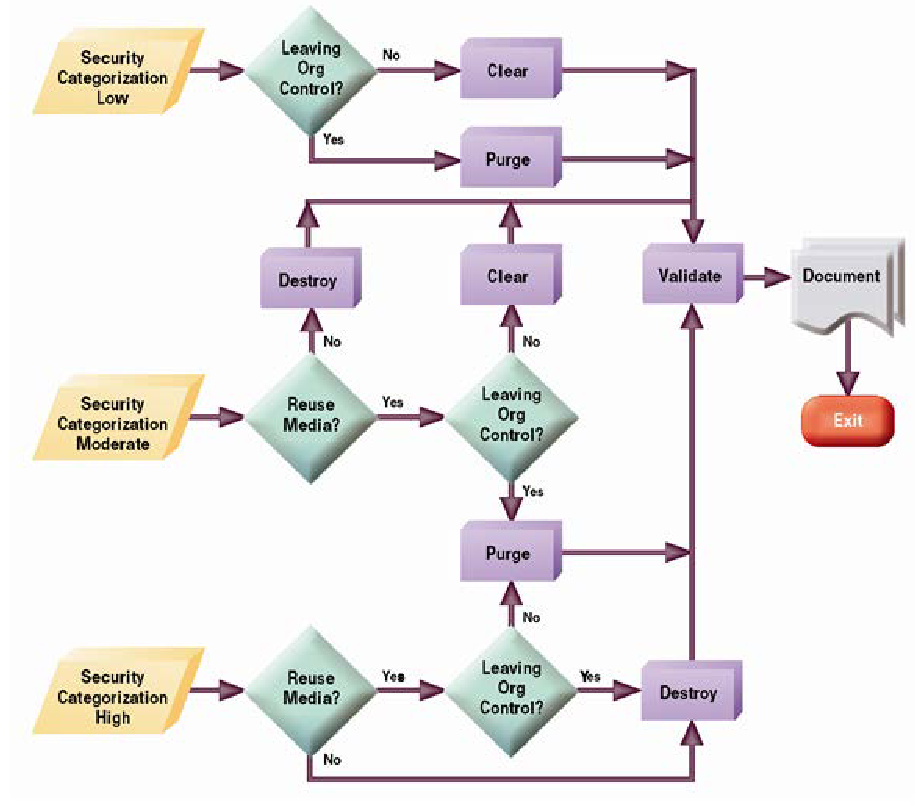
\includegraphics[width=.75\textwidth]{screen1.png}
\caption{Neo4j Browser interface}
\label{fig:neo4jbrowser}
\end{figure}

\section{Introduction to Cypher}

\paragraph*{Nodes}
Figure~\ref{fig:sample-cypher} shows how nodes and relationships are represented in the Cypher syntax. In Neo4j, nodes\index{Node (in Neo4j)} may be labelled with zero, one, or more labels. Labels\index{Label (in Neo4j)} are not types; a label does not specify anything about the information associated with a node, it merely serves to categorize or classify nodes. Nodes may have properties\index{Property (in Neo4j)}, specified as key--value pairs in JSON syntax. Graph nodes are written with normal round parentheses, with the set of their properties in curly brackets. Both the variable name for the node and the node labels are optional.

\begin{cyphercode}
(variable : Label1:Label2:Label3 ... {k1:v1, k2:v2, k3:v3 ....})
\end{cyphercode}


\begin{figure}
\centering
\includegraphics[width=.75\textwidth]{sample-cypher.png}
\scriptsize{\url{https://neo4j.com/docs/getting-started/_images/sample-cypher.svg}}
\caption{Sample Cypher syntax}
\label{fig:sample-cypher}
\end{figure}

\paragraph*{Relationships} Relationships\index{Relationship (in Neo4j)} are directed connections between two nodes. Unlike nodes, relationships only have a single label. But like nodes, they can have properties specified as key--value pairs in JSON syntax. Relationships are written as ''lines'' between nodes, directed or undirected, with an optional variable name and relationship label in square brackets. 

\begin{samepage}
\begin{cyphercode}
// Undirected, used in pattern
()-[variable : Label]-()  
// Directed 
()-[variable : Label]->() 
// Directed
()<-[variable : Label]-() 
// Unlabelled, no variable
()-[]-()    
()-->()
()<--()
\end{cyphercode}
\end{samepage}

\begin{tcolorbox}[colback=alert]
\emph{Only directed relationships can be created in a Neo4j graph, but undirected relationships can be used in a pattern to query a graph}. \\

Directionality of relationships is important and matters for querying a graph. A directed relationship \texttt{-->} will match a directed pattern \texttt{-->} or an undirected pattern \texttt{--} but not \texttt{<--}. 
\end{tcolorbox}

\paragraph*{Path}
A path\index{Path (in Neo4j)} in Neo4j is a sequence of alternating nodes and relationships, beginning and ending with a node.

\paragraph*{Patterns and Querying}

Graph patterns\index{Pattern (in Cypher)} are used with the MATCH query keyword and describe either a node or a path that is to be searched for in the graph. When an instance of a pattern is found, any variable names in the pattern are bound to the corresponding nodes and relationship in the graph and the bound pattern is returned in the result set.

For example, consider the following simple pattern matching query. The \texttt{MATCH} clause specifies the pattern to match. The pattern here is a node, indicated by the use of round parentheses, and only a variable name \texttt{n} is specified, no labels or property values. This means that this pattern matches all nodes in the graph database and returns them in the variable names \texttt{n}.

\begin{cyphercode}
MATCH (n)
\end{cyphercode}

The next pattern matching query adds a label \texttt{Person} to the node specification. This means the pattern matches only those nodes that are labelled as Person and returns them in the variable named \texttt{p}.

\begin{cyphercode}
MATCH (p:Person)
\end{cyphercode}

Patterns can include property values to match. The following pattern matches all Person nodes that contain an attribute \texttt{name} with value 'Joe' and returns them in the variable \texttt{p}.

\begin{cyphercode}
MATCH (p:Person {name: 'Joe'})
\end{cyphercode}


\section{Defining Graphs in Cypher}

Nodes or relationships in a graph can be created using the MERGE or CREATE statements in Cypher. As the name indicates, CREATE will create a node or relationship. In contrast, MERGE will check whether the node or relationship exists and only create it when it does not yet exist in the graph. Consider the example graph shown in Figure~\ref{fig:johnsallyexample}. The following Cypher codes creates this graph:

\begin{figure}[h]
\centering
\includegraphics[width=.75\textwidth]{screen4.png} \\

\scriptsize{\url{https://neo4j.com/docs/getting-started/_images/modeling_johnsally_properties-arr.svg}}
\caption{Example graph}
\label{fig:johnsallyexample}
\end{figure}

\begin{samepage}
\begin{cyphercode}
// Create nodes
MERGE (j:Person {name: "John"})
  ON CREATE SET j.age = 27
MERGE (s:Person {name: "Sally"})
  ON CREATE SET s.age = 32
MERGE (b:Book {title: "Graph Databases"})
  ON CREATE SET b.authors = ["Jim Webber", "Ian Robinson"]
  
// Create relationships
MERGE (j)-[rel1:IS_FRIENDS_WITH]->(s)
  ON CREATE SET rel1.since = "01/09/2013"
MERGE (j)-[rel2:HAS_READ]->(b)
  ON CREATE SET rel2.on = "02/03/2013", rel2.rated = 5
MERGE (s)-[rel3:HAS_READ]->(b)
  ON CREATE SET rel3.on = "02/09/2013", rel3.rated = 4
\end{cyphercode}
\end{samepage}

Note that the six \texttt{MERGE} statements in the above code block are logically related, so that variable names, for example \texttt{j, b} and \texttt{s}, in one \texttt{MERGE} clause can be used to refer to a new node or relationship in a later \texttt{MERGE} clause. While using variable names in a \texttt{MERGE} clause is not mandatory, it is more efficient than having to later query the graph data for a particular node when creating subsequent relationships. The \texttt{ON CREATE SET} clause in the above statements sets one or more property values (separated by commas) of the newly created nodes and relationships. Note that some properties are lists, such as the \texttt{authors} property, indicated by the square brackets of the JSON notation. 

The following \texttt{MATCH} queries can be used to view all nodes and relationships, irrespective of their labels. The first \texttt{MATCH} clause matches all nodes and returns them, the second \texttt{MATCH} clause matches all relationships between any two nodes and returns the relationships, the final query matches any two nodes that are connected by a relationship and returns the set of triples of first node, second node, and relationship.

\begin{samepage}
\begin{cyphercode}
// Query nodes
MATCH (n) RETURN n    
                
// Query relationships
MATCH ()-[r]-() RETURN r              

// Query both together
MATCH (n1)-[r]-(n2) RETURN n1, r, n2  
\end{cyphercode}
\end{samepage}

\noindent The Neo4j Browser interface allows graph visualization and visual exploration of nodes, relationships, and their properties, as shown in Figure~\ref{fig:neo4jgraphviz}.

\begin{figure}[h]
\centering
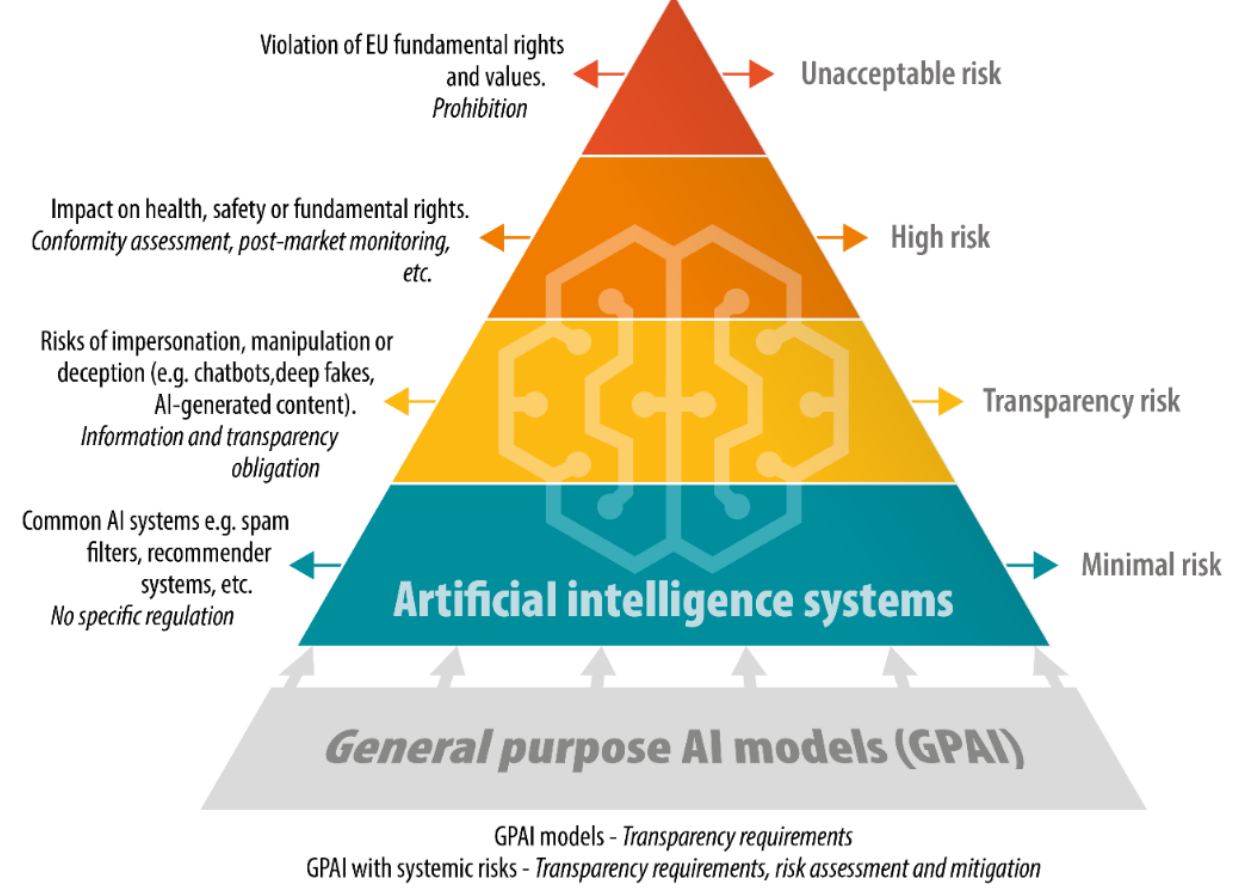
\includegraphics[width=.8\textwidth]{screen2.png}
\caption{Graph Visualization and Exploration in Neo4j Browser}
\label{fig:neo4jgraphviz}
\end{figure}

\begin{tcolorbox}[colback=code]
\subsubsection*{Hands-On Exercise}

Consider the following description:

\begin{quote}
''You are completing the course BUSI 4720 in this semester with a final grade of 100. BUSI 4720 is part of the BCom program where it is offered in the 4th year. BUSI 4720 carries 3 credit hours of academic credit. It is a course on the topic of Business Analytics.''
\end{quote}

Define a graph in Cypher that represents this description:
\begin{enumerate}
  \item Identify nodes, relationships, and properties of nodes and relationships
  \item Use CREATE or MERGE statements to create nodes first, then relationships
  \item Use MATCH to verify your graph is correct.
\end{enumerate}
\end{tcolorbox}

To remove nodes and relationships from a graph, use the \texttt{MATCH} query clause together with a \texttt{DELETE} clause. For example, to clean and remove the Person and Book nodes and relationships between Person and Book nodes created in the previous exercise, use the following Cypher statements:

\begin{cyphercode}
MATCH (:Person|Book)-[r]-(:Person|Book) DELETE r;
MATCH (n:Person|Book) DELETE n;
\end{cyphercode}

To remove \emph{all} relationships and nodes, irrespective of their label, omit node or relationship labels, as in the following Cypher code block. Use with care as this deletes all data in the graph database.

\begin{cyphercode}
MATCH ()-[r]-() DELETE r;
MATCH (n) DELETE n;
\end{cyphercode}

\section{Graph Data Modeling}

When defining a graph, one frequent question is whether to model something as a property of a node or as a relationship to a node. While there is no generally right or wrong answer to this question, the choice of data model depends on the queries to be run against the data, that is, the type of questions that will be asked.

\subsection*{Nodes versus Relationships}

Consider the two graph models in Figures~\ref{fig:propertymodel} and \ref{fig:relationshipmodel}. Both depict the same fact, that there exists a movie with title ''The Matrix'' in two genres, ''Action'', and ''Sci-Fi''. Figure~\ref{fig:propertymodel} models the genres as a property of list type, that contains multiple entries in the list. In contrast, Figure~\ref{fig:relationshipmodel} models the genres as nodes and the fact that the movie is in a genre as a relationship between the movie node and a genre node.

\begin{figure}
\centering
\begin{subfigure}{0.48\textwidth}
    \includegraphics[width=.95\textwidth]{screen5.png}
    \scriptsize{\url{https://neo4j.com/docs/getting-started/\_images/modeling\_genre\_property-arr.svg}}
    \caption{Model as property}
    \label{fig:propertymodel}
\end{subfigure}
\hfill
\begin{subfigure}{0.48\textwidth}
    \includegraphics[width=.95\textwidth]{screen6.png}
    \scriptsize{\url{https://neo4j.com/docs/getting-started/\_images/modeling\_genre\_node-arr.svg}}
    \caption{Model as relationship}
    \label{fig:relationshipmodel}
\end{subfigure}
\hfill
\caption{Equivalent graph models of movie genres}
\label{fig:equivalentmodels}
\end{figure}

The graph model in Figure~\ref{fig:propertymodel} is particularly useful to find the genres for a particular movie, that is, it is useful for queries that focus on the nodes and their properties. However, this model makes it difficult, cumbersome, and inefficient to find movies that share genres. The system has to consider all pairs of movies, and then for each pair of movies iterate through each of their property lists. The following two queries exemplify this. The first query simply filters the Movie nodes for a particular title and returns the genre attribute of the Movie node. 

The second query first identifies all pairs of Movie nodes in the \texttt{MATCH} clause, then uses the \texttt{WHERE} clause to filter those pairs that share entries in their genre attribute. Recall that the genre attributes are lists, so \texttt{x IN m1.genre WHERE x IN m2.genre} checks every element of the second list for every element of the first list. 

\begin{samepage}
\begin{cyphercode}
// find the genres for a particular movie
MATCH (m:Movie {title:"The Matrix"})
RETURN m.genre;

// find which movies share genres
MATCH (m1:Movie), (m2:Movie)
WHERE any(x IN m1.genre 
          WHERE x IN m2.genre)
AND m1 <> m2
RETURN m1, m2;
\end{cyphercode}
\end{samepage}

The graph model in Figure~\ref{fig:relationshipmodel} on the other hand requires a more complex query to find the genres of the movie. However, while more complex, it no less efficient than the corresponding query for the other model above. On the other hand, the query to find movies that share genres becomes easier, more intuitive to write, and more computationally efficient, as the following Cypher queries show.

The first query uses \texttt{MATCH} to first select movies and filter on the movie name, then for that movie \texttt{m} it traverses the \texttt{IN\_GENRE} relationship to identify all related Genre nodes \texttt{g} in order to return their names. The second query is more intuitive than the corresponding query for the other model. It finds two Movie nodes \texttt{m1} and \texttt{m2} that both have an \texttt{IN\_GENRE} relationship that points to the same Genre node \texttt{g}. 

\begin{samepage}
\begin{cyphercode}
// find the genres for a particular movie
MATCH (m:Movie {title:"The Matrix"}),
      (m)-[:IN_GENRE]->(g:Genre)
RETURN g.name;

// find which movies share genres
MATCH (m1:Movie)-[:IN_GENRE]->(g:Genre),
      (m2:Movie)-[:IN_GENRE]->(g)
RETURN m1, m2, g
\end{cyphercode}
\end{samepage}

In summary, neither way of modeling the facts is better or worse, but the two options are more suitable to different types of queries and data to be retrieved.

\begin{figure}
\centering
\begin{subfigure}{\textwidth}
    \centering
    \includegraphics[width=.5\textwidth]{screen7.png} \\
    \scriptsize{\url{https://neo4j.com/docs/getting-started/_images/modeling_airport_flights-arr.svg}}
    \caption{Airports and their relationship}
    \label{fig:flexiblegraph1}
\end{subfigure}
\hfill
\begin{subfigure}{\textwidth}
    \centering
    \includegraphics[width=.75\textwidth]{screen8.png} \\
    \scriptsize{\url{https://neo4j.com/docs/getting-started/_images/modeling_airport_flight_dates-arr.svg}}
    \caption{Modeling days as relationship labels}
    \label{fig:flexiblegraph2}
\end{subfigure}
\hfill
\caption{Graph models of airports and flights}
\label{fig:airportmodels}
\end{figure}

\subsection*{Labels versus Attributes} 

Consider the two graph models in Figures~\ref{fig:flexiblegraph1} and \ref{fig:flexiblegraph2}. The two models demonstrate the flexibility of modeling connected data and using labels to simplify queries and make them more efficient.

Figure~\ref{fig:flexiblegraph1} shows \texttt{Airport} nodes connected by \texttt{:FLYING\_TO} relationships that indicate that a flight exists from one to the other airport. Information about flights is modelled as properties of the relationship. However, noting that multiple flights may be offered each day, it is clear that a flight node is required to represent each of those flights, with a node property that represents the date of the flight. However, when querying such a model for flights on a particular date, the system must examine all flight nodes, and then filter those with the appropriate property value for the data. 

A more efficient model is that shown in Figure~\ref{fig:flexiblegraph2}. Here, the date of the flight is modelled as a label for the relationship between \texttt{Airport} and \texttt{AirportDay} nodes, which allows the system to easily select only those flights that occur on a certain date without having to examine all flight nodes. 

This example shows again that the queries to be run against the data have a strong impact on how best to model your data, here affecting the decision whether to model data as an attribute or a label.

\subsection*{Relational Model and Graph Model}

The relational data model consists of tables, their columns, and foreign key relationships that link tables (Figure~\ref{fig:relationalgraph1}). It is straightforward to translate such a model to a graph model using the following translation heuristics:

\begin{itemize}
  \item Table names become node labels
  \item Rows of data become nodes
  \item Columns become node properties
  \item Foreign keys become relationships between nodes
  \item Join tables become relationships between nodes; their properties become relationship properties
  \item Null values do not become properties, they are omitted entirely
\end{itemize}

\begin{figure}
\centering
\begin{subfigure}{\textwidth}
    \centering
    \includegraphics[width=.75\textwidth]{screen9.png} \\
    
    \scriptsize{\url{https://neo4j.com/docs/getting-started/_images/relational_model.svg}}
    \caption{A relational model}
    \label{fig:relationalgraph1}
\end{subfigure}
\hfill
\begin{subfigure}{\textwidth}
\centering
\includegraphics[height=2in]{screen10.png} \\

\scriptsize{\url{https://neo4j.com/docs/getting-started/_images/relational_graph_model-arr.svg}}
    \caption{An equivalent graph model}
    \label{fig:relationalgraph2}
\end{subfigure}
\hfill
\caption{Transforming relational data to graph data}
\label{fig:relationalgraph}
\end{figure}

Applying these heuristics to the example in Figure~\ref{fig:relationalgraph1} leads to the graph model in Figure~\ref{fig:relationalgraph2}. The table names ''Employee'' and ''Department'' have become node labels for two different categories of nodes. Each row in the employee table (for example, employee 815 with name Alice) is represented as a node with label \texttt{Person}, and each department (for example, department 111 with name 4Future) is a node with label \texttt{Department}. The column names, the ''name'' column in the Employees table and the ''deptName'' column in the Departments table, have become properties of the corresponding nodes. The ''Dept\_Members'' table joins employees and departments and has been transformed into the relationship with label \texttt{BELONGS\_TO} between \texttt{Person} and \texttt{Department} nodes. The ''Dept\_Members'' table had no columns other than those participating in the foreign key relations, but if it had, those columns would be attributes on the \texttt{BELONGS\_TO} relationship.

Applying these heuristics should only be considered as an initial translation. As seen above, some or all properties may well be represented as nodes in their own right (Figure~\ref{fig:equivalentmodels}) or be modelled as relationship labels (Figure~\ref{fig:airportmodels}), depending on the type of queries expected to be run against the graph data.

\paragraph*{Pagila Database Example} As an example, each table of the Pagila relational database from the previous chapter was exported from PostgreSQL to a CSV file. These CSV files can be imported into Neo4j with the following set of Cypher expressions. Note that not all data is imported in this example, and a more compact representation of the statements is possible. 

\begin{tcolorbox}[colback=alert]
The Pagila database is already imported into the Neo4j Community Edition in the course virtual machine.
\end{tcolorbox}

\FloatBarrier

\begin{cyphercode}
load csv with headers from 'file:///actor.csv' as row 
merge (actor:Actor {actorID: row.actor_id})
on create set actor.firstName = row.first_name 
on create set actor.lastName = row.last_name;

load csv with headers from 'file:///address.csv' as row
merge (address:Address {addressID: row.address_id})
on create set address.address = row.address
on create set address.district = row.district
on create set address.postalCode = row.postal_code
on create set address.phone = row.phone;

load csv with headers from 'file:///category.csv' as row
merge (category:Category {categoryID: row.category_id})
on create set category.name = row.name;

load csv with headers from 'file:///city.csv' as row
merge (city:City {cityID: row.city_id})
on create set city.city = row.city;

load csv with headers from 'file:///country.csv' as row
merge (country:Country { countryID: row.country_id})
on create set country.country = row.country;

load csv with headers from 'file:///customer.csv' as row
merge (customer:Customer { customerID: row.customer_id})
on create set customer.firstName = row.first_name
on create set customer.lastName = row.last_name
on create set customer.email = row.email;

load csv with headers from 'file:///film.csv' as row
merge (film:Film { filmID: row.film_id})
on create set film.title = row.title
on create set film.releaseYear = toInteger(row.release_year)
on create set film.rentalDuration = toInteger(row.rental_duration)
on create set film.rentalRate = toFloat(row.rental_rate)
on create set film.length = toInteger(row.length)
on create set film.rating = row.rating;

load csv with headers from 'file:///inventory.csv' as row
merge (inventory:Inventory { inventoryID: row.inventory_id });

load csv with headers from 'file:///language.csv' as row
merge (language:Language { languageID: row.language_id })
on create set language.name = row.name;

load csv with headers from 'file:///payment.csv' as row
merge (payment:Payment { paymentID: row.payment_id } )
on create set payment.amount = toFloat(row.amount)
on create set payment.paymentDate = row.payment_date;

load csv with headers from 'file:///rental.csv' as row
merge (rental:Rental { rentalID: row.rental_id } )
on create set rental.rentalDate = row.rental_date
on create set rental.returnDate = row.return_date;

load csv with headers from 'file:///staff.csv' as row
merge (staff:Staff { staffID: row.staff_id }) 
on create set staff.firstName = row.first_name
on create set staff.lastName = row.last_name
on create set staff.email = row.email;

load csv with headers from 'file:///store.csv' as row
merge (store:Store { storeID: row.store_id });
//
// Foreign keys
//
load csv with headers from 'file:///address.csv' as row
match (address:Address { addressID: row.address_id} )
match (city:City { cityID: row.city_id} )
merge (address)-[r:ADDRESS_CITY]->(city);

load csv with headers from 'file:///city.csv' as row
match (city:City { cityID: row.city_id} )
match (country:Country { countryID: row.country_id } )
merge (city)-[r:COUNTRY_OF_CITY]->(country);

load csv with headers from 'file:///customer.csv' as row
match (customer:Customer { customerID: row.customer_id} )
match (store:Store {storeID: row.store_id} )
match (address:Address { addressID: row.address_id} )
merge (customer)-[r1:CUSTOMER_STORE]->(store)
merge (customer)-[r2:CUSTOMER_ADDRESS]->(address);

load csv with headers from 'file:///film.csv' as row
match (language:Language { languageID: row.language_id} )
match (film:Film { filmID: row.film_id} )
merge (film)-[r:FILM_LANGUAGE]->(language);

load csv with headers from 'file:///inventory.csv' as row
match (inventory:Inventory { inventoryID: row.inventory_id} )
match (film:Film { filmID: row.film_id} )
match (store:Store { storeID: row.store_id} )
merge (store)-[r1:STORE_INVENTORY]->(inventory)
merge (film)-[r2:FILM_INVENTORY]->(inventory);

load csv with headers from 'file:///payment.csv' as row
match (payment:Payment { paymentID: row.payment_id} )
match (customer:Customer { customerID: row.customer_id} )
match (staff:Staff { staffID: row.staff_id} )
match (rental:Rental { rentalID: row.rental_id} )
merge (payment)-[r1:PAYMENT_CUSTOMER]->(customer)
merge (payment)-[r2:PAYMENT_STAFF]->(staff)
merge (payment)-[r3:PAYMENT_RENTAL]->(rental);

load csv with headers from 'file:///rental.csv' as row
match (rental:Rental {rentalID: row.rental_id} )
match (inventory:Inventory {inventoryID: row.inventory_id} )
match (customer:Customer {customerID: row.customer_id} )
match (staff:Staff {staffID: row.staff_id} )
merge (rental)-[r1:RENTAL_INVENTORY]->(inventory)
merge (rental)-[r2:RENTAL_CUSTOMER]->(customer)
merge (rental)-[r3:RENTAL_STAFF]->(staff);

load csv with headers from 'file:///staff.csv' as row
match (staff:Staff {staffID: row.staff_id} )
match (address:Address {addressID: row.address_id} )
match (store:Store {storeID: row.store_id} )
merge (staff)-[r1:STAFF_ADDRESS]->(address)
merge (staff)-[r2:STAFF_STORE]->(store);

load csv with headers from 'file:///store.csv' as row
match (store:Store {storeID: row.store_id} )
match (staff:Staff {staffID: row.manager_staff_id} )
match (address:Address {addressID: row.address_id} )
merge (store)-[r1:STORE_MANAGER]->(staff)
merge (store)-[r2:STORE_ADDRESS]->(address);
//
// Join tables for foreign keys
//
load csv with headers from 'file:///film_actor.csv' as row
match (actor:Actor {actorID: row.actor_id} )
match (film:Film {filmID: row.film_id} )
merge (actor)-[r:ACTS_IN]->(film);

load csv with headers from 'file:///film_category.csv' as row
match (film:Film {filmID: row.film_id} )
match (category:Category {categoryID: row.category_id} )
merge (film)-[r:FILM_CATEGORY]->(category);
\end{cyphercode}

Importing the Pagila database takes about 10 minutes and will yield a graph that can be explored visually using Neo4j Browser using the following Cypher command that calls a built-in function for visualizing the database schema. A screen shot of the visual explorer is shown in Figure~\ref{fig:pagilagraph}.

\begin{cyphercode}
CALL db.schema.visualization()
\end{cyphercode}


\begin{figure}
\includegraphics[width=\textwidth]{screen13.png}
\caption{The Pagila database in Neo4j Browser}
\label{fig:pagilagraph}
\end{figure}

\begin{tcolorbox}[colback=alert]
When importing from files, or exporting to files, Neo4j Community Edition uses the the \texttt{/var/lib/neo4j/import/} directory on the server. Files to import must be placed in that directory, and exported files will be created there. Additionally, any scripts to be run by calling \texttt{CALL apoc.cypher.runFile()} must be located in that directory.
\end{tcolorbox}

\section{Graph Queries with Cypher}

This section introduces the syntax of Cypher queries using example queries for the Pagila database as imported in the previous section.

\paragraph*{Example:}
Find actors by last name, limit to 10.

\begin{samepage}
\begin{cyphercode}
MATCH (a:Actor) 
RETURN a.firstName, a.lastName
ORDER BY a.lastName DESC
LIMIT 10;
\end{cyphercode}
\end{samepage}

The Cypher code above shows basic node label matching in the \texttt{MATCH} clause, returning a selection of node properties using the \texttt{RETURN} clause, ordering and limiting the result set using the \texttt{ORDER BY} and \texttt{LIMIT} clause, which are analogous to the SQL clauses with the same names.

\paragraph*{Example:} Find films whose title starts with a 'T' and that have a rental rate less than 3, sort by film title, limit to 10.

\begin{samepage}
\begin{cyphercode}
MATCH (f:Film {rating: "PG"})
WHERE (f.title STARTS WITH "T") AND (f.rentalRate < 3)
RETURN f.title, f.rating, f.rentalRate
ORDER BY f.title ASC LIMIT 10;
\end{cyphercode}
\end{samepage}

The Cypher code above introduces note matching on labels and properties and filterung using a \texttt{WHERE} clauses. Two conditions are combined using the \texttt{AND} word. Note that the matching on the rating property value of 'PG' could also have been incorportated into the \texttt{WHERE} clause, but not all WHERE clause conditions can always be moved to the node property specification in the \texttt{MATCH} clause and queries may be more readable when using a \texttt{WHERE} clause. 

\paragraph*{Example:} Find rental datas and customer names of customers that live in India.

\begin{samepage}
\begin{cyphercode}
MATCH (r:Rental) 
        -[:RENTAL_CUSTOMER]->(c) 
        -[:CUSTOMER_ADDRESS]->() 
        -[:ADDRESS_CITY]->()
        -[:COUNTRY_OF_CITY]->(ct {country: "India"})
RETURN c.firstName, c.lastName, r.rentalDate LIMIT 5
\end{cyphercode}
\end{samepage}

This example introduces matching of paths that contain multiple nodes and multiple relationships. In the above query, the types or labels or nodes and relationships are specified, but because no properties of the intermediate nodes or relationships are to be returned, they do not need to be bound to query variables.


\begin{tcolorbox}[colback=code]
\subsubsection*{Hands-On Exercise}

Write a Cypher query to find all customers that have rented a film with rating ''PG'':

\begin{enumerate}
  \item Explore the graph visually in Neo4j browser, note the relationship types (see Figure~\ref{fig:explorerelationships})
  \item Consider the path from customer to film via rental and inventory
  \item Design a pattern that starts with a customer node and ends with a film node
  \item Define an appropriate \texttt{WHERE} clause of property restrictions in node patterns
\end{enumerate}
\end{tcolorbox}

\begin{figure}
\includegraphics[width=\textwidth]{screen14.png}
\caption{Exploring relationships among nodes in Neo4j Browser}
\label{fig:explorerelationships}
\end{figure}

\paragraph*{Example:} Find the mean and standard deviation of rental payments by country.

\begin{samepage}
\begin{cyphercode}
MATCH (p:Payment) 
        -[:PAYMENT_RENTAL]->(r:Rental) 
        -[:RENTAL_CUSTOMER]->(c) 
        -[:CUSTOMER_ADDRESS]->() 
        -[:ADDRESS_CITY]->()
        -[:COUNTRY_OF_CITY]->(ct)
WITH ct, 
     avg(p.amount) AS amountMean, 
     stDev(p.amount) AS amountSD
RETURN ct.country, amountMean, amountSD
ORDER BY amountMean DESC LIMIT 5
\end{cyphercode}
\end{samepage}

This example introduces \textbf{aggregation}. In contrast to aggregation in SQL where grouping variables must be declared in the \texttt{GROUP BY} cluase, grouping in Cypher is implicit and uses all non-aggregated variables. In the following example, the non-aggregated variables is \texttt{ct} (the country). The query also introduces the aggregation functions \texttt{avg()} and \texttt{stDev()} that compute the average and standard deviation, respectively. More information of aggregation functions can be found in the Neo4j documentation\footnote{\url{https://neo4j.com/docs/cypher-manual/current/functions/aggregating/}}.

\paragraph*{Example:} Find the sets of last names of the movie cast, and the total number of actors.

\begin{samepage}
\begin{cyphercode}
MATCH (a:Actor)-[:ACTS_IN]->(f:Film) 
RETURN f.title, 
       collect(a.lastName) AS cast, 
       count(*) AS numActors;
\end{cyphercode}
\end{samepage}

This example introduces aggregation into collections (lists) using the \texttt{collect()} function. The query returns a list of actor last names as cast, together with the count of actors that act in each movie. Grouping happens implicitly for each variable not aggregated. In this example, that is the variable \texttt{f}, representing the film.

\paragraph*{Example:} Find the set of film titles by rental customer and the number of rentals.

\begin{samepage}
\begin{cyphercode}
MATCH (f:Film)-[:FILM_INVENTORY]-()
      -[:RENTAL_INVENTORY]-(r:Rental)
      -[:RENTAL_CUSTOMER]->(c:Customer)
RETURN c.lastName, 
       collect(f.title) AS filmRentals, 
       count(*) AS numRentals;
\end{cyphercode}
\end{samepage}

This example also uses aggregation with collection and a slightly more complex graph pattern in the \texttt{MATCH} clause\footnote{From \url{https://neo4j.com/docs/getting-started/cypher-intro/results/}}.

\paragraph*{Example:} Find the set of rental customers for each film and the rental count.

\begin{samepage}
\begin{cyphercode}
MATCH (f:Film)-[:FILM_INVENTORY]-()
      -[:RENTAL_INVENTORY]-(r:Rental)
      -[:RENTAL_CUSTOMER]->(c:Customer)
RETURN DISTINCT f.title, 
      collect(c.lastName" "+left(c.firstName,1)+".") AS custNames, 
      count(*) as rentalCount
\end{cyphercode}
\end{samepage}

This example introduces string functions and operators. Strings can be concatenated with the ''+'' operator. The function \texttt{left(., n)} returns the leftmost segment of $n$ characters of the string. In contrast to the last query, here the collection creates a list of customers, grouped by films, rather than films, grouped by customer. The query also introduces the DISTINCT key word that limits the result set to unique values of a variable.

\paragraph*{Example:} Find the customers who rent films that are in inventory at multiple stores.

\begin{samepage}
\begin{cyphercode}
MATCH (c:Customer)<-[:RENTAL_CUSTOMER]-(r:Rental)
       -[:RENTAL_INVENTORY]-()
       -[:FILM_INVENTORY]-(f:Film) 
WITH c, count{ 
  MATCH (f)-[:FILM_INVENTORY]-()
        -[:STORE_INVENTORY]-(s:Store) 
  RETURN DISTINCT s.storeID } AS storeNum
WHERE storeNum > 1
RETURN DISTINCT 
  c.lastName+" "+left(c.firstName,1)+"." AS custName, 
  storeNum
\end{cyphercode}
\end{samepage}

This example introduces \emph{sub-queries} and the \texttt{WITH clause}. The \texttt{WITH} clause introduces elements that will be passed to subsequent clauses. In this example, the result of the subquery within the \texttt{\{ \ldots \}} function is passed on in the variable \texttt{storeNum} in the ''outer'' query. This is then used in the \texttt{WHERE} clause of the outer query.

\paragraph*{Example:} Find Christian Akroyd's co-actors.

\begin{samepage}
\begin{cyphercode}
MATCH (a:Actor {firstName:"CHRISTIAN", lastName:"AKROYD"}) 
      -[:ACTS_IN]->(f:Film)<-[:ACTS_IN]-(coActors) 
RETURN coActors.firstName+" "+coActors.lastName AS Name;
\end{cyphercode}
\end{samepage}

This query example emphasizes path matching from a given node. Note the second \texttt{ACTS\_IN} relationship is traversed in reverse order, it's arrow points ''left''.

\paragraph*{Example:} Movies and actors up to 2 ''hops'' away from Christian Akroyd.

\begin{cyphercode}
MATCH (a:Actor {firstName:"CHRISTIAN", lastName:"AKROYD"})
      -[:ACTS_IN*1..2]-(others:Actor) 
RETURN distinct others;
\end{cyphercode}

This query introduces \emph{quantified relationships}. In the example, the \texttt{ACTS\_IN} relationship may be traversed between 1 and 2 two times on the way to other actor nodes. Note that no Film nodes or other relationships need to be specified here.

\paragraph*{Example:} The shortest path of an acts-in relationship between Christian Akroyd and Charlize Dench.

\begin{samepage}
\begin{cyphercode}
MATCH path=shortestPath( 
  (a1:Actor {firstName:"CHRISTIAN", lastName:"AKROYD"}) 
  -[:ACTS_IN*]-(a2:Actor {firstName:"CHARLIZE", lastName:"DENCH"})) 
RETURN path;
\end{cyphercode}
\end{samepage}

This query introduces the use of \emph{built-in functions}. In this case, the built-in function \texttt{shortestPath()} is a graph-theoretic function that computes the shortest path along \texttt{ACTS\_IN} relationships between two specific nodes. Graph databases are particularly useful and efficient for queries on such graph-theoretic functions, which are very difficult to express in SQL.

\paragraph*{Example:} Find actors that Christian Akroyd hasn't yet worked with, but his co-actors have. Extend Christian Akroyd's co-actors, to find co-co-actors who haven't worked with him.

\begin{samepage}
\begin{cyphercode}
MATCH (a1:Actor {firstName:"CHRISTIAN", lastName:"AKROYD"})
         -[:ACTS_IN]->(m)<-[:ACTS_IN]-(coActors),
      (coActors)-[:ACTS_IN]->(m2)<-[:ACTS_IN]-(cocoActors)
WHERE NOT (a1)-[:ACTS_IN]->()<-[:ACTS_IN]-(cocoActors) 
      AND a1 <> cocoActors
RETURN cocoActors.firstName+" "+
       cocoActors.lastName AS Recommended, 
       count(*) AS Strength 
ORDER BY Strength DESC
\end{cyphercode}
\end{samepage}

This query example introduces the use of multiple patterns in the \texttt{MATCH} clause that are separated by commas and are related in the sense that variables in one can be used in the other and refer to the same node or relationship. The two patterns in the \texttt{MATCH} clause are connected through the shared variable \texttt{coActors}. Note also that traversal direction of the various relationships. Finally, this example also introduces the use of patterns in the \texttt{WHERE} clause, allowing more complex filters on the results. The patterns in the \texttt{WHERE} clause are also logically related to the patterns in the \texttt{MATCH} clause, in this example they share the variable \texttt{cocoActors}.

\paragraph*{Example:} Find someone who can introduce Christian Akroyd to Susan Davis.

\begin{samepage}
\begin{cyphercode}
MATCH (a1:Actor {firstName:"CHRISTIAN", lastName:"AKROYD"})
        -[:ACTS_IN]->(m)<-[:ACTS_IN]-(coActors),
      (coActors)-[:ACTS_IN]->(m2)
        <-[:ACTS_IN]-(a2:Actor {firstName:"SUSAN", lastName:"DAVIS"})
RETURN a1, m, coActors, m2, a2
\end{cyphercode}
\end{samepage}

The example is similar to the one above with its use of multiple path patterns in the \texttt{MATCH} clause. The query finds common co-actors of two named actors. Note the traversal directions of the relationships.

\begin{tcolorbox}[colback=code]
\subsubsection*{Hands-On Exercises}

The following hands-on exercises are designed to familiarize you with the Cypher language and use the Pagila database.

\begin{enumerate}[nosep]
	\item Are there two customers that have the same address?
	\item Which customers have rented the same set of films?
	\item Find all films with a single actor
	\item Calculate the rental revenue per customer. Who are the top 5? Bottom 5?
	\item Calculate the rental counts for each country of customer. Are there countries with no rentals?
	\item Create a graph that represents a product hierarchy.
\end{enumerate}
\end{tcolorbox}

\section{Review Questions}

\begin{enumerate}[nosep]
	\item What is a graph database, and how does it differ from traditional relational databases?
	\item Describe the different data models used in NoSQL databases. How does the graph model specifically cater to certain types of data and applications?
	\item Explain how data is represented in a graph database. What are nodes and relationships?
	\item List and explain the key benefits of using graph databases over traditional relational databases.
	\item How do graph databases handle relationships differently, and why is this advantageous for certain applications?
	\item Give examples of specific industries or applications where graph databases are particularly useful. Explain why a graph database is chosen over other types of databases in these scenarios.
	\item What are some of the prominent query languages used with graph databases? Briefly describe their unique features.
	\item How does Cypher, the query language for Neo4j, compare to SQL in terms of syntax and capabilities?
	\item Discuss the characteristics of Cypher as a query language. How does it enable efficient querying and manipulation of graph data?
	\item Reflect on a scenario or a problem where you think a graph database would be more effective than a traditional relational database. Explain your reasoning.
    \item Describe what a node represents in Neo4j and how it is represented in Cypher syntax.
    \item Explain how properties are associated with nodes in Neo4j. Give an example using Cypher syntax.
	\item Discuss the significance of relationship directionality in Neo4j. What is the difference between directed and undirected relationships in querying?
	\item Define what a 'pattern' is in Cypher and its role in querying the graph database.
	\item Provide an example of a simple Cypher pattern and explain what it matches in the graph.
	\item Differentiate between the `CREATE` and `MERGE` statements in Cypher. Under what circumstances would you use each?
	\item Give an example of how to create a node with multiple labels and properties using Cypher.
	\item How would you create a relationship between two nodes, including setting properties on the relationship?
	\item Explain the difference between modeling data as a property of a node versus as a separate node connected by a relationship. Give an example to illustrate your point.
	\item In the context of Neo4j, why might it be more efficient to model certain data as relationships between nodes rather than as properties of a single node? Provide an example where this is the case.
	\item Given a graph model where movie genres are modeled as properties of a movie node, what are the limitations of this approach when trying to find movies with shared genres?
	\item Describe the process of translating a relational data model into a graph model in Neo4j.
\end{enumerate}




\graphicspath{{class05/}}
\chapter{Introduction to Data Management with R}
%
% Unless otherwise indicated, the copyright in this material is 
% owned by Joerg Evermann. This material is licensed to you under the 
% Creative Commons by-attribution non-commercial license (CC BY-NC 4.0)}
%
\section*{Learning Goals}

After reading this chapter, you should be able to:
\begin{itemize}
   \item Create and manipulate basic data structures in R, including arrays, matrices, and data frames.
   \item Create summary information from R data frames and other data structures.
   \item Use the Tidyverse packages to retrieve information from R data frames, including filtering, grouping, and aggregation of information.
   \item Use SQL to operate on R data frames to retrieve information, including filtering, grouping, and aggregation of information.
\end{itemize}


\section*{Sources and Further Reading}

The material in this chapter is based on the following sources. 

\begin{resourcebox}
Venables, W.N., Smith, D.M. and the R Core Team (2024) An Introduction to R.  \\

\footnotesize
\url{https://cran.r-project.org/doc/manuals/r-release/R-intro.pdf}\normalsize
\end{resourcebox}

This tutorial is a good, easy, and comprehensive introduction to R. It covers the most important aspects of R in 100 pages. It is continuously updated by the R team for new versions of R and new features. Chapters 1 through 7 cover the initial material in this module. 

\begin{resourcebox}
Wickham, H., Cetinkaya-Rundel, M., and Grolemund, G. (2023) R for Data Science. O'Reilly Media, Inc. \\

\footnotesize\url{https://r4ds.hadley.nz/}\normalsize
\end{resourcebox}

This is a free, open-source book directly from the authors of the popular and widely-used Tidyverse libraries. With many examples, and easy-to-understand descriptions, the book provides a solid foundation for business analytics with R. It provides sections on data import, data transformation, data visualization, and data communication, each with multiple chapters. This is a highly relevant resource for anyone doing data science in R.

\begin{resourcebox}
Posit (2024) Cheatsheet. \\

\footnotesize\url{https://posit.co/resources/cheatsheets/}\normalsize
\end{resourcebox}

Posit is the maker of the popular RStudio programming environment for R, the shiny library for building web applications and graphical dashboards with R, and a number of other open-source and proprietary tools around the R system. Posit provides a number of very helpful ''cheatsheets'' that are one-page summaries of various R libraries. The ''cheatsheets'' useful for this module is the one on the dplyr package for data transformation.


\section{Introduction}

R is a statistical software system and programming language known for its robust capabilities in data analysis, visualization, and statistical computing. It was originally developed in the early 1990s by Ross Ihaka and Robert Gentleman at the University of Auckland, New Zealand. Drawing inspiration from the S language developed at Bell Laboratories, R was designed to be a powerful and flexible tool for data analysis and statistical modeling.

One of the key advantages of R is its open-source nature, making it freely available to users worldwide. This accessibility has created a vibrant community of users and developers, continuously enhancing its functionality through comprehensive packages and extensions. The Comprehensive R Archive Network (CRAN) is a repository of these packages, offering tools for a myriad of data analysis tasks.

R's popularity stems not only from its wide range of statistical techniques, including linear and nonlinear modeling, time-series analysis, classification, clustering, and others, but also from its exceptional capabilities in data visualization. The software provides an integrated suite of tools for data manipulation, calculation, and graphical display, making it an invaluable asset for statisticians, researchers, and data scientists.

Moreover, R's programming language aspect allows for automation and customization in data analysis, which is highly beneficial for complex and repetitive tasks. Its compatibility with various data formats and integration with other programming languages and tools further enhances its versatility.

\section{Using R}

R is a command-line oriented software, that is, users type commands to perform calculations or call functions of R packages. A sequence of R commands can be assembled in a \emph{script file}, so that they may be re-run when necessary. The advantage of this type of software over one with a graphical user interface is in the repeatability and replicability of the work. Ideally, data analysts will assemble an R script file for their entire data analysis, from reading the raw data sets to the finished statistical analyses and visualizations, so that all details of the analysis are available for replication and evaluation.

\begin{figure}
\centering
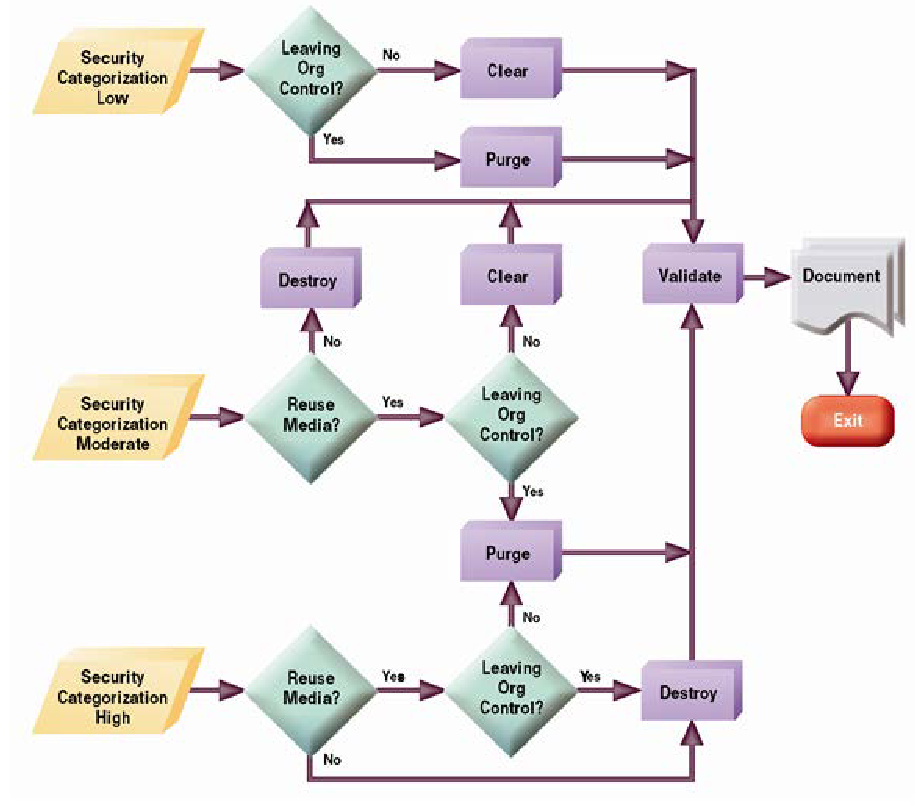
\includegraphics[width=.8\textwidth]{screen1.png}
\caption{The R command line interface}
\label{fig:r}
\end{figure}

The R system can be launched simply by invoking the \texttt{R} command from the terminal window, as shown in Figure~\ref{fig:r}. R will display its version information and prompt for command entry with a \texttt{>} prompt. 

To install R on Microsoft Windows or on MacOS, download the installation files from CRAN (Comprehensive R Archive Network) at \url{https://cran.r-project.org} and follow the instructions. R on Microsoft Windows and R on MacOS will show their command prompts inside a window but otherwise function similarly to R on Ubuntu that is installed in the course virtual machine.

\begin{infobox}
To make using R more efficient, consider doing the following:

\begin{itemize}
    \item Use the {\footnotesize\colorbox{lightgray}{up-arrow}} key to retrieve earlier commands.
    \item The \texttt{history()} function shows your command history.
    \item Use a notepad app to assemble and edit your commands easily, then copy/paste to R for execution.
    \item Use a notepad app for your results, copy/paste from R.
    \item The Ubuntu terminal uses {\footnotesize\colorbox{lightgray}{SHIFT-CTRL-X}}, {\footnotesize\colorbox{lightgray}{SHIFT-CTRL-C}}, {\footnotesize\colorbox{lightgray}{SHIFT-CTRL-V}} for cut/copy/paste.
    \item Use multiple terminal and R windows (e.g. one for executing commands, one for reading help documentation or for listing files).
    \item Don't update packages in the middle of a project.
    \item Ensure you have a \emph{repeatable, automatable script} for your entire data analysis at the end of a project.
\end{itemize}
\end{infobox}

\section{R Basics}

The most basic way to use R is to simply use it as a calculator, as shown in the following R code example. Type ''\texttt{1+1}'' at the ''\texttt{>}'' prompt, then press the \colorbox{lightgray}{RETURN} key to execute the statement. R will respond on the following line with the result:

\begin{Rcode}
> 1+1
[1] 2
\end{Rcode}

A \emph{variable} in R is a named storage space for numbers, characters, strings, and other data elements. Traditionally, values are assigned to variables using the \texttt{<-} operator, but one may also use the more ''normal'' assignment operator \texttt{=}. Using the \texttt{<-} assignment operator helps to clearly distinguish assignment from equality testing, which uses \texttt{==}. 

The following R code example introduces the R function called \texttt{print()} that does as its name suggests. Most data types and data structures that can be assigned to variables have a useful print function associated to them, so that on the interactive R command line you can simply type their name to get their value. In interactive mode, R calls the \texttt{print()} function automatically. In an R script that you execute from file, you will have to explicitly use the \texttt{print} function.

\begin{Rcode}
> a <- 3
> b <- 2
> print(a * b)
[1] 6
> a
[1] 3
\end{Rcode}

R has special symbols to denote infinity (\texttt{inf}) and results that are not a number (\texttt{NaN}):

\begin{Rcode}
> 2 / 0
[1] Inf
> 0 / 0
[1] NaN
\end{Rcode}

\noindent The boolean logical operators \emph{and} and \emph{or} are represented by the operators \texttt{\&} and \texttt{|} shown in the R code block below.

\begin{Rcode}
> TRUE & FALSE
FALSE
> TRUE | FALSE
TRUE
\end{Rcode}

\begin{infobox}
The boolean constants \texttt{TRUE} and \texttt{FALSE} can be abbreviated by \texttt{T} and \texttt{F}
\end{infobox}

Character strings in R are enclosed in single or double quotes (but not mixed quotes!). Two useful functions are \texttt{paste()} which pastes its arguments together with an optional separator between them and returns a characters string, and the \texttt{strsplit()} function which accepts a string (or vector of strings) to split, and a separator character that identifies where to split the string. It returns a list of vectors of strings.

\begin{Rcode}
> label1 = 'I Love R'
> label2 = 'and BUSI 4760'
> paste(label1, label2, sep=' ')
> strsplit('Hello World! My first string', ' ')
\end{Rcode}

Because you can assign arbitrary values to variables in R, R provides functions to test the type of the value and to coerce, that is, to change, the type of a value.

\begin{Rcode}
# Check whether it is numeric
is.numeric(2)
# Check whether it is an integer number
is.integer(3.14)
# Make it an integer
as.integer(3.14)
# Make it a character string
as.character(3.14)
# Make it a character string
as.character(TRUE)
# Make it a number
as.numeric('3.1415')
\end{Rcode}

\section{The R Environment}

The collection of variables, functions, and libraries that exists in R at any one time is called the R \emph{workspace}. The functions \texttt{ls()} and \texttt{rm()}, named after their Unix bash shell equivalents, list and remove objects from the R workspace.

\begin{Rcode}
# Show objects in workspace
> ls()
[1] "a"          "b"
# Remove one object
> rm(b)
> ls()
[1] "a"
\end{Rcode}

R comes with a built-in user manual that one can access with the \texttt{help()} function or simply the \texttt{?} operator. Help is available on any function in R, as shown in the following example. For added convenience, R provides a web browser interface to its help pages that is started by \texttt{help.start()}.

\begin{Rcode}
help()
help(lm)
?lm
??lm
help.start()
\end{Rcode}

R has a current working directory where it reads and writes files from and to. On Ubuntu Linux, this is the directory from which the \texttt{R} command was issued. R provides functions to get the working directory (\texttt{getwd()}), to set (change) it (\texttt{setwd()}, and to list the files in the working directory (\texttt{list.files()}):

\begin{Rcode}
# Get the working directory
getwd()
# Set the working directory
setwd('DataSets')
getwd()
# List files in working directory
list.files()
\end{Rcode}

\begin{infobox}It is often more convenient to change the working directory in the terminal, prior to invoking \texttt{R}.
\end{infobox}

A collection of related functions is called a \emph{library} in R. While some libraries come with the base R system, other packages will need to be downloaded and installed. The CRAN (Comrehensive R Archive Network) provides libraries in convenient form. To install packages from CRAN, use the \texttt{install.packages()} function with the name (or a vector of names) of packages to install from CRAN. Once installed, libraries can be attached to the R workspace with the \texttt{library()} function, which makes its functions and any data sets it contains available for use. 

\begin{Rcode}
# Install the tidyverse library
install.packages('tidyverse')
# Load/attach the tidyverse library
library(tidyverse)
# List all installed packages
installed.packages()
\end{Rcode}

It is sometimes useful to assemble a series of related R commands for a particular data analysis task in a script file. Script files are useful to ensure that the analysis can be repeated. The \texttt{source()} function will read and execute a file containing R commands. As noted earlier, in a script file, you will need to use the \texttt{print()} function to print the values of variables.

\begin{Rcode}
source('MyFirstScript.R')
\end{Rcode}

Finally, the \texttt{quit()} function ends an R session. When using \texttt{quit()} without arguments, R will ask whether to save the workspace image. R stores its \emph{workspace} in each directory in a file called ''.RData'' and will read it when restarted from that directory. R also stores its \emph{command history} in each directory in a file called ''.Rhsitory'' and will read it when restarted from that directory.

\begin{Rcode}
quit()
\end{Rcode}

\section{Vectors}

A common structured data type in R is a \emph{vector}\index{Vector (in R)}. A vector in R contains elements of the same data type and is ordered. When assigning elements of different datatypes to a vector, R will coerce the types of all elements to a common datatype.

\begin{Rcode}
> v <- c(1, 'a', TRUE)
> v
[1] "1"    "a"    "TRUE"
> v <- c(1, 2, 3, 4)
> v*3
[1]  3  6  9 12
\end{Rcode}

In the above example, R automatically determined that multiplication with a scalar is an element-wise operation and applies it to each element of the vector. 

Useful functions to create vectors are the sequence function \texttt{seq()}, which accepts the lower and upper limit and a step size as parameter, and the repetition function \texttt{rep()} which repeats its first argument the number of times specified by its second argument.

\begin{Rcode}
# Generate a sequence
s <- seq(0, 6, by=.5)
print(s)
# Repeat a value
r <- rep(3.5, 5)
print(r)
\end{Rcode}

R provides useful functions for numerical vectors, to find their length, their maximum and minimum value, the square root of their values, as well as the variance and standard deviation of the elements. R automatically determines whether functions are applied to the whole vector, like \texttt{var()} or \texttt{sd()}, or whether functions are applied element-wise to each element, like \texttt{sqrt()}. Vector concatenation, using the \texttt{c()} function, automatically ''flattens'' the vectors.

\begin{Rcode}
length(v)
max(v)
min(v)
sqrt(v)
var(v)
sd(v)
# Vectors get flattened
vv <- c(v, c(7, 8, 9), v)
print(vv)
\end{Rcode}

The most common way to select elements from vectors is by \emph{indexing} with a boolean vector. In the following example, the expression \texttt{vv < 5} yields a vector of boolean values (true or false). Indexing the variable \texttt{vv} with that vector determines which elements of \texttt{vv} to select (those elements for which the corresponding entry is true).

\begin{Rcode}
vv < 5
vv[vv < 5]
vv[vv < 5] <- vv[vv < 5] + 5
\end{Rcode}

Vectors can also be indexed numerically, selecting elements by their position. This is also called ''Slicing''. R allows you select a sequence of values with the \texttt{:} operator, and the exclusion of elements, or sequences of elements, using \texttt{-}. The first line in the following example selects elements at positions 3 through 7, the second line selects elemnts \emph{except} those at positions 3 through 7.

\begin{Rcode}
# Indexing is inclusive
vv[3:7]
vv[-(3:7)]
\end{Rcode}

\begin{alertbox}
\begin{itemize}
   \item R begins indexing positions with 1, while other programming languages begin at 0.
   \item Indexing in R is inclusive, that is, both the start and end index are included.
\end{itemize}
\end{alertbox}

\emph{Missing values} are designated by the special symbol \texttt{NA}. The \texttt{is.na()} function can be used to identify and select \texttt{NA} and then filter them. When an aggregation function encounters a \texttt{NA}, it will normally return a \texttt{NA}, so it is important to remove or replace \texttt{NA} values before analyzing the data. Many functions offer an option to remove \texttt{NA} values prior to applying them, as shown for the \texttt{sum()} function in the following R code block. 

\begin{Rcode}
# Introduce a missing value
v[3] <- NA
# Missing value arithmetic
v*3
# Testing for missing values
is.na(v)
# Missing values in aggregate functions
sum(v)
sum(v, na.ram=TRUE)
\end{Rcode}

Important string functions are \texttt{grep()} and \texttt{agrep()}. The \texttt{grep()} function checks whether each string in a vector of strings contains a substring that matches a regular expression, and returns the indices of strings in the vector that match the pattern. The first use of \texttt{grep()} in the following R code block matches a phone number, the second use of \texttt{grep()} matches a Canadian postal code.

\begin{Rcode}
# Match/find North American phone numbers
> grep('^([0-9]{3})[ -]?[0-9]{3}[ -]?[0-9]{4}$', 
    c('709 864 5000', 'abc def 9999', '709-865-5000'))
[1] 1 3
# Match/find Canadian postal codes
> grep('[A-V][0-9][A-V] [0-9][A-V][0-9]', 
    c('A0P 1L0', '0AB L2K', 'A0X 1Z0'))
[1] 1
\end{Rcode}

The \texttt{agrep()} function calculates the Levenshtein distance between a regular expression and a vector of strings and returns the indices of those strings that are within a certain distance. The Levenshtein distance is defined as the sum of insertions, deletions, and substitutions of characters to transform one string into another.

\begin{Rcode}
# Match/find strings up to Levenshtein distance of 3
> agrep('apple', 
    c('apricot', 'banana', 'grape', 'pineapple'), 
    max.distance=3)
[1] 1 3 4
\end{Rcode}

\section{Arrays, Matrices, and DataFrames}

R \emph{arrays}\index{Array (in R)} are multi-dimensional objects that can hold any primitive data type, usually numerical. A \emph{matrix}\index{Matrix (in R)} is simply a two-dimensional array. The following example shows how indexing (''Slicing'') generalizes from vectors to matrices and arrays simply by indexing each dimension with the same syntax as used for vectors. The \texttt{array()} function creates multi-dimensional arrays from existing data, the \texttt{dim()} function returns the number of dimensions of an array.

A few important things to note in the following R code block example:
\begin{itemize}
   \item The first dimension is the row, the second is the column
   \item Initially, the array is created from a range of numbers between 1 and 20, and the \texttt{dim} argument specifies the dimensionality. 
   \item R fills arrays by column, unless otherwise specified
   \item A dimension need not be slided or indexed, as in \texttt{a[,2]} or \texttt{a[,2:4]} which do not subset the first dimension (rows). The result is that all rows are returned in these examples. 
   \item Reversing the index reverses the result that is returned, as in \texttt{a[3:1,2:4]} which reverses the indexing of the first dimension (rows). 
\end{itemize}

\begin{Rcode}
# Default is to fill by column
a <- array(1:20, dim=c(4,5))
a
# Result:
#      [,1] [,2] [,3] [,4] [,5]
# [1,]    1    5    9   13   17
# [2,]    2    6   10   14   18
# [3,]    3    7   11   15   19
# [4,]    4    8   12   16   20
# Indexing is inclusive and starts at 1
a[,2]
a[,2:4]
a[3,2:4]
a[3:1,2:4]
\end{Rcode}

Constructing a \emph{matrix} with the \texttt{matrix()} function is similar to constructing an array, but instead of providing the dimensionality with \texttt{dim}, one must provide either the number of rows or columns (\texttt{nrow} or \texttt{ncol}) and how to fill the matrix from the elements provided using the \texttt{byrow} argument; by default, R fills arrays and matrices by column. 

The \texttt{t()} function returns the transpose of a matrix, that is, it reverses rows and columns. Binding (combining) two matrices together by columns with \texttt{cbind()} or by rows with \texttt{rbind()} requires compatible dimensions, that is, same number of rows for \texttt{cbind()} or same number of columns for \texttt{rbind()}.

\begin{Rcode}
b <- matrix(20:1, nrow=5, byrow=T)
b
# Result:
#      [,1] [,2] [,3] [,4]
# [1,]   20   19   18   17
# [2,]   16   15   14   13
# [3,]   12   11   10    9
# [4,]    8    7    6    5
# [5,]    4    3    2    1
# Test if it is a matrix
is.matrix(b)
is.matrix(a)
# Transpose
t(b)
# Bind (combine) by columns
cbind(a, t(b))
# Bind (combine) by rows
rbind(t(a), b)
\end{Rcode}

A \emph{data frame}\index{Data frame!in R} is the most widely used data structure for data analytics and statistics in R. It is essentially a table with a set of columns whose elements are of the same type. Columns are named and columns can be selected using the \texttt{\$} symbol. Useful functions on data frames are \texttt{summary()}, \texttt{head()} and \texttt{tail()}. 

The following R code block creates a variable \texttt{x} as a vector of 50 normally distributed random values using the \texttt{rnorm()} function. The variable \texttt{y} is created from vector \texttt{x} and then adds a normally distributed random variable. The two are then combined into a data frame with the \texttt{data.frame()} function. The \texttt{colnames()} function retrieves the column names, but can also change/update the column names. The \texttt{nrow()} and \texttt{ncol()} functions return the number of rows and columns, \texttt{head()} and \texttt{tail()} return the first few or last few rows, and \texttt{cov()} is an example of a statistical function that returns the covariance matrix of all columns in the data frame.

\begin{Rcode}
# Create a vector of 50 normally distributed random variables
x <- rnorm(50)
# Create another vector with random variables
y <- 2*x + rnorm(50)
# Create a data frame from the two vectors
data <- data.frame(x, y)
#  Get the column names
colnames(data)
# Update the column names
colnames(data) <- c('Pred', 'Crit')
# Get the number of rows and columns
nrow(data)
ncol(data)
# Get the "Pred" column of the data frame
data$Pred
# Print a summary
summary(data)
# Print first and last rows
head(data)
tail(data)
# Calculate the covariance matrix
cov(data)
\end{Rcode}

Data frames may be written to CSV files and read from CSV files, as shown in the following R code block. The functions \texttt{write.csv()} and \texttt{read.csv()} have a range of options for reading/writing files with or without header lines, with different separators, for skipping rows, for different decimal points, for whitespace stripping, etc. Consult the R built-in help system for details.

\begin{Rcode}
# Write CSV file into current working directory
# Omit the row names
write.csv(data, 'data.csv', row.names=FALSE)
# Read the data from the current working directory
new.data <- read.csv('data.csv')
\end{Rcode}

\begin{exercisebox}
These hands-on exercises are designed to familiarize you with the Tidyverse packages, especially the dplyr package. Use these exercises with the Pagila CSV data set.

\begin{enumerate}[nosep]
    \item Create an array with $3$ columns and $50$ rows of random numbers with mean of $2$ and standard deviation of $4$ (use the \texttt{rnorm()} function)
   \item Create a dataframe from the array and name the columns as ''A'', ''B'', ''C''
   \item ''Clip'' the values so that all values lie between $-3$ and $+7$
   \item Summarize the data
   \item Print the pairwise covariance matrix of the three columns in the data frame
   \item Find the square root of each of the diagonal entries of the covariance matrix, compare this to the standard deviation of 4. Tip: Use the \texttt{diag()} function.
   \item Save the data frame in a CSV file using your first name as file name (file ending '.csv')
\end{enumerate}
\end{exercisebox}

\section{Tidyverse}

The Tidyverse is a collection of R libraries designed for data science that share an underlying design philosophy, grammar, and data structures. Developed by Hadley Wickham and others, the Tidyverse libraries are built to work together seamlessly, making data science tasks more straightforward and intuitive. At the core of Tidyverse's philosophy is the concept of ''tidy data,'' which arranges data in a structured way that simplifies analysis. This structure involves organizing data into rows and columns where each variable is a column, each observation is a row, and each type of observational unit forms a table.

Key libraries in the Tidyverse include \emph{ggplot2} for data visualization, \emph{dplyr} for data manipulation, \emph{tidyr} for data tidying, \emph{readr} for reading data, \emph{purrr} for functional programming, and \emph{tibble} for providing a better version of a table data structure. In particular, ggplot2 allows for complex and aesthetically pleasing visualizations using a layered grammar of graphics (hence the name), while dplyr provides a set of tools for efficiently manipulating datasets, such as filtering rows, selecting columns, and aggregating data. Tidyr helps in transforming messy data into a tidy format, making it easier to analyze and visualize. Table~\ref{tab:tidyverse} contains a summary of the libraries.

\begin{table}
\centering

\renewcommand{\arraystretch}{1.25}
\begin{tabular}{l|l} \hline
dplyr & Manipulate data \\
forcats & Work with categorical variables (factors) \\
ggplot2 & Grammar of Graphics \\
lubridate & Date and time parsing and arithmetic \\
purrr & Functional programming \\
readr & Read files in various formats \\
stringr & Work with character strings \\
tibble & A tibble is better than a table \\
tidyr & Make data tidy \\ \hline
\end{tabular}
\caption{Tidyverse packages for R}
\label{tab:tidyverse}
\end{table}

Tidyverse also emphasizes readability and expressiveness in code, which not only makes data analysis easier to write but also easier to read and understand. It has become a popular choice among data scientists and statisticians for its ease of use, efficiency, and the cohesive way it handles data analysis tasks. The integration of these packages under the Tidyverse umbrella simplifies the process of data manipulation, exploration, and visualization, greatly enhancing the productivity and effectiveness of data analysis in R.

Loading and attaching the \texttt{tidyverse} library in R, using the \texttt{library(tidyverse)} function, loads all the associated core packages, as shown in Figure~\ref{fig:tidyverse}.

\begin{figure}
\centering
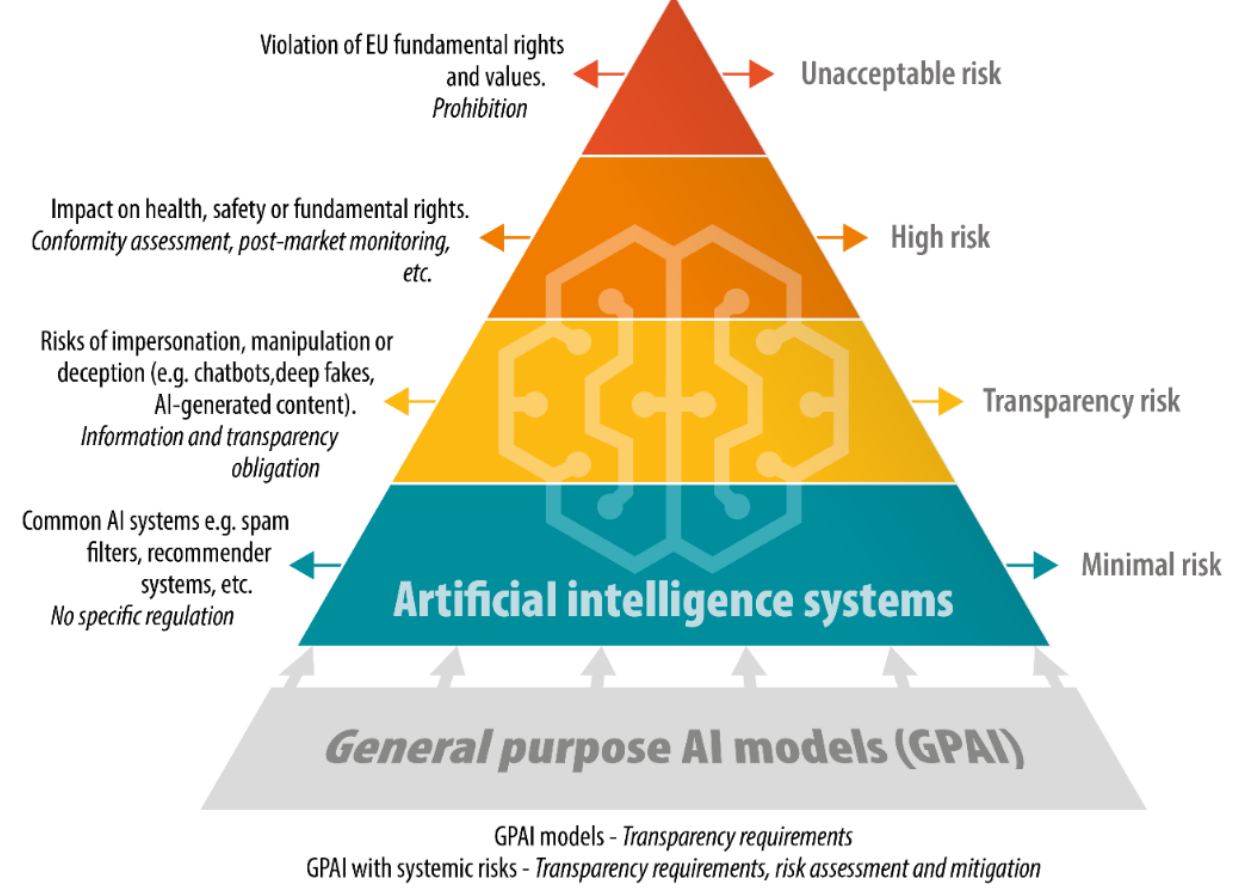
\includegraphics[width=\textwidth]{screen2.png}
\caption{Attaching the tidyverse packages in R}
\label{fig:tidyverse}
\end{figure}

\subsection*{Tidyverse Basics}

This subsection introduces basic ideas of data manipulation with the Tidyverse package, primarily using the dplyr package. A simple data set is used to illustrate basic functionality. The example dataset for this section is the Fuel Consumption Ratings for battery electric vehicles, provided the Government of Canada through its Open Government Portal\footnote{\scriptsize\url{https://open.canada.ca/data/en/dataset/98f1a129-f628-4ce4-b24d-6f16bf24dd64}}. The dataset contains the variables shown in Table~\ref{tab:fueldatachapter5}.

\begin{table}[h]
\centering
\renewcommand{\arraystretch}{1.25}

\begin{tabularx}{.9\linewidth}{|l|l|X|} \hline
  {\bf Column} & {\bf Data Type} & {\bf Definition} \\ \hline \hline
  Make & Categorical (string) & Manufacturer \\ 
  Model & Categorical (string) & Model name\\
  Year & Numeric & Model year \\
  Category & Categorical (string) & Small, Midsize, Large, Pickup, SUV, Station Wagon, etc. \\
  City & Numeric & Consumption in l/100km equiv. \\
  Hwy & Numeric & Consumption in l/100km equiv. \\
  Comb & Numeric & Consumption in l/100km equiv. \\
  Range & Numeric & Driving range in km \\ \hline
\end{tabularx}
\caption{Fuel efficiency data set variables}
\label{tab:fueldatachapter5}
\end{table}

\paragraph*{Reading Data:} When reading CSV files with readr, the data is stored in a \emph{tibble}\index{Tibble}, not a data frame. A tibble provides a number of extensions and convenience operations that make it much more capable than a data frame. When using data frames with any dplyr function, they are automatically converted to tibbles. 

The following R code reads a CSV file using the \texttt{read\_csv()} function from the Tidyverse readr library (not the \texttt{read.csv()} function from basic R!) and prints the first few lines and a summary. 

When reading CSV files with readr, the data is stored in a \emph{tibble}\index{Tibble}, not a data frame. A tibble provides a number of extensions and convenience operations that make it much more capable than a data frame. When using data frames with any dplyr function, they are automatically converted to tibbles. The output looks slightly different than that for data frames, but accomplishes essentially the same things.

\begin{Rcode}
# Read CSV into a Tibble
data <- read_csv('https://evermann.ca/busi4720/fuel.csv')
# Examine the data
# Dimensions (rows, columns)
dim(data)
# Column names
colnames(data)
# Summary
summary(data)
\end{Rcode}

The functionality in the dplyr library is intended to mirror SQL queries from the earlier module on relational databases. The main dplyr ''verbs'' used in the examples are summarized in Table~\ref{tab:dplyr}. The examples below will illustrate each of these ''verbs'' or functions and also show the equivalement SQL statements. 

\begin{table}
\centering
\renewcommand{\arraystretch}{1.25}

\begin{tabularx}{\textwidth}{l|X} \hline
\multicolumn{2}{c}{Basic} \\ \hline
\texttt{filter} & filters by row \\
\texttt{select} & selects columns to retain \\
\texttt{mutate} & creates new columns \\
\texttt{rename} & renames columns \\
\texttt{distinct} & finds unique values \\
\texttt{arrange} & sorts data rows \\
\texttt{relocate} & moves data columns \\
\texttt{group\_by} & groups data \\
\texttt{summarize} & compute aggregate information \\
\texttt{print} & prints a tibble \\  \hline
\multicolumn{2}{c}{Advanced} \\ \hline
\texttt{nest} & nests data, tibbles in tibbles \\
\texttt{full\_join} & Joins tibbles (also \texttt{outer join}, \texttt{left\_join}, \texttt{inner\_join}, \texttt{right\_join}) \\ \hline
\end{tabularx}
\caption{Important dplyr functions}
\label{tab:dplyr}
\end{table}

The tidyverse libraries make extensive use of the \emph{pipe}\index{Pipe} operator in R. The pipe operator allows chaining of function calls and plugs the result of one function as the first argument into the next function. 

\paragraph*{Filtering:} The example below starts with the tibble that was read earlier and pipes it into the \texttt{filter()} function. The filter function specifies two conditions, filtering data by vehicle Make and vehicle model Year. The output of the \texttt{filter} function is piped into the \texttt{print()} function. 

\begin{Rcode}
# Pipe a data frame or tibble into a filter and print results
data |> 
  filter(Make=='Ford', Year==2023) |> 
  print()

# Equivalent without pipe and boolean operator in filter
filter(data, Make=='Ford' & Year==2023)
\end{Rcode}

The \texttt{filter()} function is similar to the \texttt{WHERE} clause in an SQL SELECT statement and the above R code is equivalent to the following SQL statement:

\begin{sqlcode}
SELECT * 
   FROM data 
   WHERE Make=='Ford' AND Year==2023;
\end{sqlcode}

\paragraph*{Selection:} The following example adds the \texttt{select()} function to select specific columns from the data set:

\begin{Rcode}
# Pipe a data frame or tibble into a filter,
# select specific columns and print results
data |> 
  filter(Make=='Ford', Year==2023) |> 
  select(Model, Category, Range) |>
  print()
\end{Rcode}

There is no equivalent SQL clause for the \texttt{select()} function because the selection of result columns occurs in the main SELECT clause, as illustrated in the following equivalent SQL statement:

\begin{sqlcode}
SELECT Model, Category, Range 
   FROM data 
   WHERE Make=='Ford' AND Year==2023;
\end{sqlcode}

\paragraph*{Column Creation:} The next example shows the use the \texttt{mutate()} function to create a new column that expresses the range of a vehicle for highway driving. It involves a calculation using the Hwy fuel economy, the Comb combined fuel economy and the Range. The \texttt{mutate()} function is added into the above data manipulation pipeline:

\begin{Rcode}
# Pipe a data frame or tibble into a filter,
# create a new calculated column,
# select specific columns and print results
data |> 
  filter(Make=='Ford', Year==2023) |> 
  mutate(HwyRange = Range * Comb / Hwy) |>
  select(Model, Category, Range, HwyRange) |>
  print()
\end{Rcode}

An equivalent SQL statement constructs the new column in the main SELECT clause:

\begin{sqlcode}
SELECT Model, Category, Range, (Range*Comb)/Hwy AS HwyRange 
   FROM data 
   WHERE Make=='Ford' AND Year==2023;
\end{sqlcode}

\paragraph*{Renaming:} The example below shows renaming of columns using the \texttt{rename()} function. The Range column is renamed to be the CombRange column. While \texttt{mutate()} creates an additional columns, \texttt{rename()} does not and only renames an existing column. It is therefore more efficient for renaming.

\begin{Rcode}
# Pipe a data frame or tibble into a filter,
# create new calculated columns,
# rename an existing column,
# select specific columns and print results
data |> 
  filter(Make=='Ford', Year==2023) |> 
  mutate(HwyRange = Range * Comb / Hwy) |>
  mutate(CityRange = Range * Comb / City) |>
  rename(CombRange = Range) |>
  select(Model, Category, CombRange, CityRange, HwyRange) |>
  print()
\end{Rcode}

An equivalent SQL statement constructs the new column in the main SELECT clause using the AS keyword:

\begin{sqlcode}
SELECT Model, Category, 
      Range AS CombRange,
      (Range*Comb)/Hwy AS HwyRange, 
      (Range*Comb)/City As CityRange
   FROM data 
   WHERE Make=='Ford' AND Year==2023;
\end{sqlcode}

\paragraph*{Distinct Values:} The \texttt{distinct()} function can be used to find the set of unique values of a column. For example, the following R code identifies the unique vehicle Makes and Models in the data set. 

\begin{Rcode}
# Pipe a data frame or tibble into a filter,
# select distinct value combinations and print results
data |> 
  distinct(Make, Model) |>
  print()
\end{Rcode}

SQL uses the DISTINCT keyword for this purpose as well, illustrated in the following example:

\begin{sqlcode}
SELECT DISTINCT Make, Model 
  FROM data;
\end{sqlcode}

\paragraph*{Ordering:} The dplyr \texttt{arrange()} function is used to order data by values, in ascending or descending order. The following example illustrates this by adding the \texttt{arrange()} function to the data processing pipeline. The \texttt{arrange()} function orders the data first by vehicle Category in ascending order (the default ordering), then, for equal values of Model, by Range in descending order (using the \texttt{desc()} function:

\begin{Rcode}
# Pipe a data frame or tibble into a filter,
# select specific columns,
# order the data and print results
data |> 
  filter(Make=='Ford', Year==2023) |> 
  select(Model, Category, Range) |>
  arrange(Category, desc(Range)) |>
  print()
\end{Rcode}

An equivalent SQL statement uses the ORDER BY clause with the keywords ASC or DESC to indicate the direction of ordering:

\begin{sqlcode}
SELECT Model, Category, Range
   FROM data 
   WHERE Make=='Ford' AND Year==2023
   ORDER BY Category ASC, Range DESC;
\end{sqlcode}

\paragraph*{Relocating Columns:} The function \texttt{relocate()} can be used to specify the order in which columns are returned. The following code example rearranges the column order before printing by adding the \texttt{relocate()} function to the data processing pipeline:

\begin{Rcode}
# Pipe a data frame or tibble into a filter,
# select specific columns,
# order the data,
# move columns and print results
data |> 
  filter(Make=='Ford', Year==2023) |> 
  select(Model, Category, Range) |>
  arrange(Category, desc(Range)) |>
  relocate(Category, Range) |>
  print()
\end{Rcode}

SQL does not require a function or keyword in the SELECT statements. There, columns are returned in the order in which they are specified in the SELECT clause:

\begin{sqlcode}
SELECT Category, Range, Model
   FROM data 
   WHERE Make=='Ford' AND Year==2023
   ORDER BY Category ASC, Range DESC;
\end{sqlcode}

\paragraph*{Grouping and Summarizing:} The \texttt{group\_by()} function can be used to group data in preparation for computing aggregate information. It is typically used with the \texttt{summarize()} function that calculates aggregates. 

The following example shows how to compute mean fuel efficiency data, grouped by vehicle Make and vehicle Category. It adds both a \texttt{group\_by()} and a \texttt{summarize()} function into the data processing pipeline. The summarized data is then filtered again, it is sorted by vehicle Category and mean combined fuel economy, and the columns are then reordered so that vehicle Category and mean combined economy are the first two columns.

\begin{Rcode}
# Pipe a data frame or tibble into a filter,
# group the data
# summarize the data,
# filter the summary information,
# order the data,
# relocate columns and print results
data |> 
  filter(Year==2023) |> 
  group_by(Make, Category) |>
  summarize(meanCity = mean(City), 
            meanHwy = mean(Hwy),
            meanComb = mean(Comb),
            maxRange = max(Range),
            nVehicle = n()) |>
  filter(nVehicle > 1) |>
  arrange(Category, meanComb) |>
  relocate(Category, meanComb) |>
  print()
\end{Rcode}

The equivalent SQL statement also uses the GROUP BY clause. Summary information is defined in the main SELECT clause. The second \texttt{filter()} function in the R code refers to aggregate information, so that the equivalent clause in SQL is the HAVING clause:

\begin{sqlcode}
SELECT Category, 
       AVG(Comb) AS meanComb,
       Make,
       AVG(City) AS meanCity,
       AVG(Hwy) AS meanHwy,
       MAX(Range) AS maxRange,
       COUNT(*) AS nVehicle
   FROM data 
   WHERE Year==2023
   GROUP BY Make, Category
   HAVING COUNT(*) > 1
   ORDER BY Category ASC, meanComb ASC;
\end{sqlcode}

\section{Advanced Tidyverse for Data Analysis}

This section focuses on the use of dplyr to analyze data from a set of CSV files representing the data of the Pagila database. The Pagila database\footnote{\url{https://github.com/devrimgunduz/pagila}, \\
\url{https://github.com/devrimgunduz/pagila/blob/master/LICENSE.txt}} is a demonstration database originally developed for teaching and development of the MySQL RDBMS under the name Sakila\footnote{\url{https://dev.mysql.com/doc/sakila/en/}, \\
\url{https://dev.mysql.com/doc/sakila/en/sakila-license.html}}. Pagila is designed as a sample database to illustrate database concepts and is based on a fictional DVD rental store. It originally consists of several tables organized into categories like film and actor information, customer data, store inventory, and rental transactions. For this section, the Pagila data was summarized in a few related CSV files. The following R code block reads the data and coerces data types as required.

\begin{Rcode}
rentals <- read_csv('http://evermann.ca/busi4720/rentals.csv')
rentals$rating <- as.factor(rentals$rating)
rentals$language <- as.factor(rentals$language)
rentals$customer_address <- as.integer(rentals$customer_address)
rentals$customer_store <- as.integer(rentals$customer_store)
rentals$rental_staff <- as.integer(rentals$rental_staff)
rentals$payment_staff <- as.integer(rentals$payment_staff)
rentals$rental_duration <- as.integer(rentals$rental_duration)

actors <- 
  read_csv('https://evermann.ca/busi4720/actors.categories.csv')
  
addresses <- read_csv('https://evermann.ca/busi4720/addresses.csv')
addresses$phone <- as.character(addresses$phone)
\end{Rcode}

The following paragraphs show further examples of data analysis with Tidyverse and introduce additional dplyr functions or additional ways to use the dplyr functions. These example data processing pipelines mirror the example in the previous module on SQL. Only new aspects of the examples are explained.

\paragraph*{Example:} Find all films and the actors that appeared in them, ordered by film category and year, for those films that are rated PG.

\begin{Rcode}
rentals |> 
  full_join(actors, by='title', 
    suffix=c('_customer', '_actor'), 
    relationship='many-to-many') |>
  filter(rating == 'PG') |>
  mutate(actor = 
    paste(last_name_actor, ', ', first_name_actor, sep='')) |>
  rename(year=release_year) |>
  select(actor, title, category, year) |>
  distinct(actor, title, category, year) |>
  group_by(category, year, title) |> 
  nest() |>
  arrange(category, year, title) |>
  relocate(category, year, title) |>
  print(n=Inf, width=Inf)
\end{Rcode}

This R code joins the rentals data with the actors data using a full join. The join is performed on the title column that is common to both data frames/tibbles. The \texttt{suffix} argument adds distinct suffixes to column names from each data frame to avoid name clashes. The \texttt{relationship='many-to-many'} indicates the nature of the join.

The \texttt{mutate()} function creates a new column named actor, which concatenates the actor's last name and first name, separated by a comma and a space.

The data is grouped by category, year, and title, using the \texttt{group\_by()} function, and the \texttt{nest()} function is used to create a nested data frame, i.e. a data frame where the actors for each group are in a list-valued column.

\paragraph*{Example:} Find the most popular actors in the rentals in each city.

This R code block below involves combining multiple data frames and then manipulating and summarizing the data. It builds on the rental and actor tibbles from the previous example and adds address information.

\begin{Rcode}
full_data <- 
  rentals |> 
    inner_join(addresses, by=c('customer_address'='address_id')) |>
    inner_join(actors, by='title',
      suffix=c('_customer', '_actor'),
      relationship='many-to-many')
       
full_data |> 
  mutate(actor = 
    paste(last_name_actor, ', ', first_name_actor, sep='')) |>
  group_by(city, actor) |>
  summarize(count=n()) |>
  mutate(ranking = min_rank(desc(count))) |>
  filter(ranking < 4) |>
  arrange(city, ranking, actor) |>
  print(n=25)
\end{Rcode}

The analysis starts by reading a CSV file containing address information into a tibble. An inner join is performed between the rental data and the address data, matching them on a specified key in each data frame, that is, the cusomter\_address in the rentals data frame must be equal to the address\_id in the addresses data frame. 

This is followed by another inner join with the actors data frame. No join key/column is specified as the join is done on columns that have the same name in both data frames. This second join involves a many-to-many relationship and adds suffixes to to distinguish columns with the same name in the two data frames.

The data is grouped by city and actor and a new summary column is created that counts the number of occurrences (records) for each group. To create rankings, a new column is added that ranks the groups based on their count value in descending order. The \texttt{min\_rank()} function allows ties in the ranking, use \texttt{rank()} to break ties with gaps in ranking or \texttt{dense\_rank()} to break ties with no gaps in ranking. The data is then filtered to include only those records with a ranking less than 4, focusing on the top three ranks for each group.


\paragraph*{Example:} Find the customers who spend the most on rentals, with their phone numbers and cities, and the number of rentals with the higest total rental payments for each category grouped by rental duration.

\begin{Rcode}
full_data |>
   mutate(customer= paste(first_name_customer, last_name_customer)) |>
   select(customer, amount, rental_duration, category, phone, city) |>
   group_by(category, rental_duration, customer ) |>
   mutate(payments=sum(amount), num_rentals=n()) |>
   select(-amount) |>
   group_by(category, rental_duration) |>
   mutate(ranking = min_rank(desc(payments))) |>
   slice(which.min(ranking)) |>
   print(n=Inf, width=Inf)
\end{Rcode}

In this example, there is no \texttt{summarize()} function after the \texttt{group\_by()} function because \texttt{summarize()} omits all non-grouped columns, but the example requires phone numbers and cities of customers. Either these would need to be included somehow in the \texttt{summarize()} function, or, as is done in this R code, summary columns are created using the \texttt{mutate()} function instead.  Also note the ''negative'' argument to the \texttt{select()} function, which is used to remove the ''amount'' column. The data processing pipeline uses multiple \texttt{group\_by()} statements with different aggregate functions (\texttt{sum()}, \texttt{n()}, \texttt{min\_rank()}) for the different groups. Finally, the R code uses \texttt{slice()} to select the rows with the smallest ranks.

\paragraph*{Example:} Get the total rental revenue, number of rentals, and the mean and standard deviation of the rental amounts for each country.

\begin{Rcode}
full_data |>
  group_by(country) |>
  summarize(revenue=sum(amount), 
            numrentals=n(),
            mean_amount=mean(amount),
            sd_amount=sd(amount)) |>
  arrange(desc(mean_amount),
          desc(revenue)) |>
  print(n=Inf, width=Inf)  
\end{Rcode}

The R code for this query demonstrates a number different aggregate summary functions, \texttt{sum()}, \texttt{n()}, \texttt{mean()} and \texttt{sd()} (standard deviation). It also shows how to use the \texttt{desc()} function to arrange or sort data in decreasing order.

\paragraph*{Example:} Get the top 5 and the bottom 5 grossing customers for each quarter.

\begin{Rcode}
full_data |>
  mutate(customer=paste(first_name_customer,last_name_customer)) |>
  mutate(q=as.character(quarter(rental_date, with_year=T))) |>
  select(customer, q, amount, rental_date) |>
  group_by(q, customer) |>
  mutate(payments=sum(amount)) |>
  select(-amount) |>
  distinct(customer, q, payments) |>
  group_by(q) |>
  mutate(rank_top = min_rank(desc(payments))) |>
  mutate(rank_bot = min_rank(payments)) |>
  filter(rank_top <= 5 | rank_bot <= 5) |>
  arrange(q, desc(payments)) |>
  relocate(q, customer, payments, rank_top, rank_bot) |>
  print(n=Inf, width=Inf)
\end{Rcode}

The code for this query again does not use a \texttt{summarize()} function. It also shows the use of the \texttt{quarter()} function from the ''lubridate'' library. The lubridate library contains a large range of date and time related functions. Two ranking columns are created using the \texttt{mutate()} and the \texttt{min\_rank()} functions, once in descending order to get the top ranks, and again in ascending order to get the bottom ronks. The code uses \texttt{filter()} instead of \texttt{slice()} to select the top and bottom 5 ranks (using a boolean ''or'' operator), uses \texttt{arrange()} to sort the data, and then uses \texttt{relocate()} to re-arrange the order of columns prior to printing.

\paragraph*{Example:} Find the set of film titles by rental customer and the total number rentals for each customer.

\begin{Rcode}
full_data |>
  mutate(customer=paste(first_name_customer,last_name_customer)) |>
  select(customer, title) |>
  nest(titles=title) |>
  rowwise() |> 
  mutate(rentals=nrow(titles)) |>
  mutate(unique_titles=list(distinct(titles))) |>
  select(-titles) |>
  arrange(customer) |>
  print(n=Inf, width=Inf)
\end{Rcode}

The code for this query works with nested data, that is, data with columns that contain lists, created using the \texttt{nest()} function. In this example, \texttt{nest(titles=title)} creates a columns called ''titles'' that contains a list of all the elements of the ''title'' column for each customer. The R code also demonstrates row-wise operations. Both \texttt{mutate()} functions after \texttt{rowwise()} function operate by row. Specifically, the first use of the \texttt{mutate()} function creates a new column ''rentals'' which contains the number of rows in the titles column \emph{for each row} (recall that the ''titles'' column contains lists of film title). Similarly, the second use of the \texttt{mutate()} function creates a new column ''unique\_title''that contains a list of distinct film titles from the ''titles'' column \emph{for each row}.

\section{SQL and R}

The ''sqldf'' library in R allows users to perform SQL queries on R data frames. Essentially, it provides a bridge between SQL and R\index{SQL!in R}. This integration allows users who are familiar with SQL to leverage its powerful querying capabilities directly on R data structures, without the need to switch between different tools or environments.

One of the main advantages of ''sqldf'' is its ability to handle large data frames more efficiently than some of R's native functions. By utilizing SQL queries, users can perform complex data manipulations and aggregations with ease. The package supports various SQL commands including SELECT, JOIN, ORDER BY, and GROUP BY, among others, enabling a wide range of data operations that are familiar to SQL users.

Under the hood, ''sqldf'' operates by temporarily converting data frames into databases, typically by creating an in-memory SQLite database, or, alternatively, using an existing database connection to any of a variety of RDBMS such as PostgreSQL. It then creates a table for each data frame, moves the data to the database tables, and executes SQL statements. It then moves the result set back into R as a data frame. This seamless process allows for a smooth integration of SQL's data processing capabilities within the R environment.

''sqldf'' is particularly useful for R users who are already comfortable with SQL syntax and for complex data manipulation tasks that might be more cumbersome or less intuitive in R's native syntax. Its ability to handle data frames as if they were SQL tables makes it a highly valuable tool for data analysts and statisticians who work with large datasets and require the flexibility and power of SQL within the R programming environment.

The following R code block shows a very simple example. Note that the SQL \texttt{FROM} clause recognizes data frame names; any columns used in the SQL query must be named columns from those data frames.

\begin{Rcode}
library(sqldf)
result_df <- sqldf('select distinct(title) from full_data')
\end{Rcode}

When faced between the choice of data analytics using an SQL RDBMS or R/Tidyverse, there are a number of issues to consider:

\begin{itemize}
 \item \emph{Size of data}: R is limited by the amount of main memory of the computer. While large computers may offer 128GB or more, modern RDBMS can scale massively larger, in particular when distributing databases across a cluster of computers.
 \item \emph{Access speed}: RDBMS have sophisticated indexing of tables and query planners that optimize complex queries for performance. While a dplyr analysis pipeline can also be optimized by carefully considering the order of function calls, the onus is on the data analyst to do this, while an RDBMS offer this ''out-of-the-box''.
 \item \emph{Currency}: Using an RDBMS means that analytics can be performed on operational data, that is, the most current and up-to-date data. In contrast, the use of R involves first exporting data from the operational system and then analyzing it at a later time. However, while tempting, it is not generally recommended to perform complex analytics on an operational database, as it can significantly affect performance. 
 \item \emph{Transactions}: An RDBMS ensures consistent views of data across multi-user, concurrent updates. This means that, when using an operational database, the analysis sees consistent data, whereas an exported snapshot of the data may not necessarily be consistent, depending on the export mechanism.
 \item \emph{Tools}: R has tools for statistical analysis and visualization, beyond mere reporting. So far, we have considered only simple descriptive analytics. However, when the data is to be used for sophisticated statistics or predictive analytics, it is no longer possible to do this on RDBMS.
\end{itemize}

\noindent These issues motivate the following recommendations:
\begin{itemize}
 \item Do not ''hit'' operational RDBMS for heavy-weight or frequent analytics. While it may be fine to do the occasional summary analytics on an operational database, this should not be normally done. 
 \item Regularly export consistent data from RDBMS. If up-to-date data is needed, automate the export from the database to occur at regular intervals. However, note also that exporting data has a performance impact on operational databases. 
 \item Sometimes, SQL may be the more intuitive language to specify the required analysis. In these cases, use separate in-memory or on-disk RDBMS for analytics (e.g. with \texttt{sqldf}) if desired/required. 
 \item Finally, if the size of data is too large to handle in R, consider distributed tools such as Hadoop/Spark that are made for Big Data analytics.
\end{itemize}

\begin{exercisebox}

These hands-on exercises are designed to familiarize you with the Tidyverse packages, especially the dplyr package. Use these exercises with the Pagila CSV data set.

\begin{enumerate}[nosep]
  \item Find all films with a rating of 'PG'
  \item List all customers who live in Canada (with their address)
  \item Find the average \emph{actual} rental duration for all films
  \begin{itemize}
     \item This requires date arithmetic, use the \texttt{lubridate} package
  \end{itemize}
  \item Find the average overdue time for each customer
  \begin{itemize}
     \item This requires date arithmetic, use the \texttt{lubridate} package
  \end{itemize}
  \item List all films that have never been rented
  \item List the names of actors who have played in more than 15 films
\end{enumerate}
\end{exercisebox}


\graphicspath{{class06/}}
\chapter{Introduction to Data Management with Python}
%
% Unless otherwise indicated, the copyright in this material is 
% owned by Joerg Evermann. This material is licensed to you under the 
% Creative Commons by-attribution non-commercial license (CC BY-NC 4.0)}
%
\section*{Learning Goals}

After reading this chapter, you should be able to:
\begin{itemize}
   \item Create and manipulate basic data structures in Python, includings lists, tuples, and dictionaries.
   \item Create and manipulate arrays using the Numpy package for Python, in particular, be able to use slicing to retrieve portions of an array.
   \item Create and manipulate series and data frames in the Pandas package for Python.
   \item Compute summary information and to retrieve portions of a Pandas data frame.
   \item Use Pandas to retrieve information from multiple data frames, including filtering, grouping, and aggregation of information.
\end{itemize}

\section{Introduction}

Python is a high-level, interpreted programming language known for its simplicity and readability. It was created by Guido van Rossum and first released in 1991. Python's design philosophy emphasizes code readability through the use of significant\footnote{''Significant'' in this context does not mean lots, it means that spaces at the beginning of a line, that is, line indentations, have meaning and Python code does not work the same way without those spaces.} whitespace. This unique approach has contributed to Python becoming one of the most popular programming languages in the world.

Python's standard library of functions is large and comprehensive, covering a range of programming needs including web development, data analysis, artificial intelligence, scientific computing, and more. Its simplicity and versatility allow programmers to express concepts in fewer lines of code compared to languages like C++ or Java. Additionally, Python supports multiple programming paradigms, including procedural, object-oriented, and functional programming.

One of the biggest advantages of Python is its strong community support and the vast availability of third-party packages, which extend its capabilities even further. Frameworks like Django for web development, Pandas for data analysis, and TensorFlow for machine learning are just a few examples of Python's extensive ecosystem.

Python's popularity can be attributed to its wide range of applications in various fields, such as web development, data science, artificial intelligence, scientific computing, and scripting. It's often used in academic and research settings due to its ease of learning and its ability to handle complex calculations and data manipulation. Major tech companies and organizations use Python, showcasing its reliability and robustness.

In terms of benefits, Python is known for its efficiency, reliability, and speed of development. It is often used for rapid prototyping and iterative development. Python's syntax is clean and its code is generally more readable and maintainable compared to many other programming languages. This readability makes it easier for developers to work on projects collaboratively.

Overall, Python's combination of versatility, simplicity, and powerful libraries makes it a preferred choice for both beginners and experienced developers across diverse fields. Its continued evolution and adaptation to new technologies and paradigms ensure its relevance in the fast-paced world of software development.

\begin{tcolorbox}[colback=code]
\paragraph*{Intro Tutorial:} 

A very good introduction to Python can be found at \url{https://python.swaroopch.com/}, or, as a downloadable PDF, at \url{https://github.com/swaroopch/byte-of-python/releases/}
\end{tcolorbox}

\section{Python versus R}

Python and R are two of the most popular programming languages used in data science, each with its unique strengths and applications. Python, known for its general-purpose nature, offers a more comprehensive approach to busienss analytics, allowing not just data analysis and visualization, but also the integration of data science processes into web applications, production systems, and more. Its simplicity and readability make it a go-to language for a wide range of developers, including those who are not primarily data scientists.

Python's extensive libraries like Pandas for data manipulation, NumPy for numerical computations, Matplotlib and Seaborn for data visualization, and Scikit-learn for machine learning make it a powerful tool for business analytics. Moreover, Python's capabilities in machine learning and deep learning, with libraries like TensorFlow and PyTorch, make it a preferred choice for cutting-edge applications in AI.

On the other hand, R, originally designed for statistical analysis, is highly specialized in statistical modeling and data analysis. It offers a rich ecosystem of packages for statistical procedures, classical statistical tests, time-series analysis, and data visualization. R is particularly favored for its advanced statistical capabilities and its powerful graphics for creating well-detailed and high-quality plots.

The choice between Python and R often comes down to the specific requirements of the project and the background of the business analytics team. Python is generally more versatile and better suited for integrating business analytics into larger production applications. It is also the more popular choice for machine learning projects. R, meanwhile, is excellent for pure statistical analysis and visualizing complex data sets. It's often preferred in academia and research settings where complex statistical methods are more commonly required.

Both languages have strong community support and a wealth of resources, making them continually evolving tools in the field of business analytics. Many business analysts are proficient in both, choosing the one that best fits the task at hand. In collaborative settings, it's not uncommon to see teams utilizing both Python and R, leveraging the strengths of each to achieve more comprehensive and powerful data analysis outcomes.

\section{Using Python}

The Interactive Python Shell, Jupyter Notebooks, and PyCharm IDE represent different environments for Python development, each with distinct features and use cases.

\paragraph*{Interactive Python Shell} The Python shell is the most basic and straightforward environment for Python programming. Users can type Python code and see the results instantly. The simplicity is the primary advantages of the Python shell. The immediate feedback makes it excellent for experimentation, learning Python syntax, and quick tests. There is no need for creating files or setting up a project environment. This feature is especially beneficial for beginners who are just starting to learn Python, as it provides a straightforward way to test out new concepts and functions without the overhead of more complex development environments. Figure~\ref{fig:pythonshell} shows a screenshot of the Python shell.

\begin{figure}
\centering
\includegraphics[width=.75\textwidth]{screen3.png}
\caption{The Interactive Python Shell}
\label{fig:pythonshell}
\end{figure}

While the Python shell supports all the features of the Python language. However, it lacks advanced features found in full-fledged Integrated Development Environments (IDEs), such as code completion, debugging tools, or project management, which are essential for larger projects. Its simplicity is both a strength and a limitation: while it is easy to use, it might not be the best choice for larger programming projects.

On Unbuntu Linux, simply type \texttt{python} in a terminal window to launch the Python shell. On Windows and MacOS systems, you will find applications to launch the Python shell in a window. The shell prompts you for commands with the \texttt{> > >} prompt. Simply enter the command and press the \colorbox{lightgray}{ENTER} key to execute a command. Use the \texttt{quit()} function to exit the shell. The Python shell remembers your previous commands, so you can use the up and down arrow keys to recall commands and edit them. The Python shell also performs code completion using the \colorbox{lightgray}{TAB} key, which helps speed up coding and reduce typing errors. Similar to an R session, you should use a notepad editor application to assemble commands and then copy/paste them into the Python shell, as copy/paste results into a notepad editor. This makes editing long commands easier and ensures that your analysis will be repeatable.


\paragraph*{Jupyter Notebooks} Jupyter notebooks offer a more interactive and versatile platform, particularly favored in data science and academic research. Jupyter Notebooks allow users to create and share documents that can contain ''cells'' where each cell may contain Python code, text (using Markdown), equations (using LaTeX), or visualizations. This mix of Python code, documentation, description, and results makes it ideal for data exploration, visualization, and complex analyses where explaining the process is as important as the code itself, allowing for a narrative approach to coading. While Jupyter Notebooks support various programming languages, they are predominantly used with Python. Figure~\ref{fig:jupyter} shows a screenshot of a Jupyter notebook in the JupyterLabs Desktop environment.

\begin{figure}
\centering
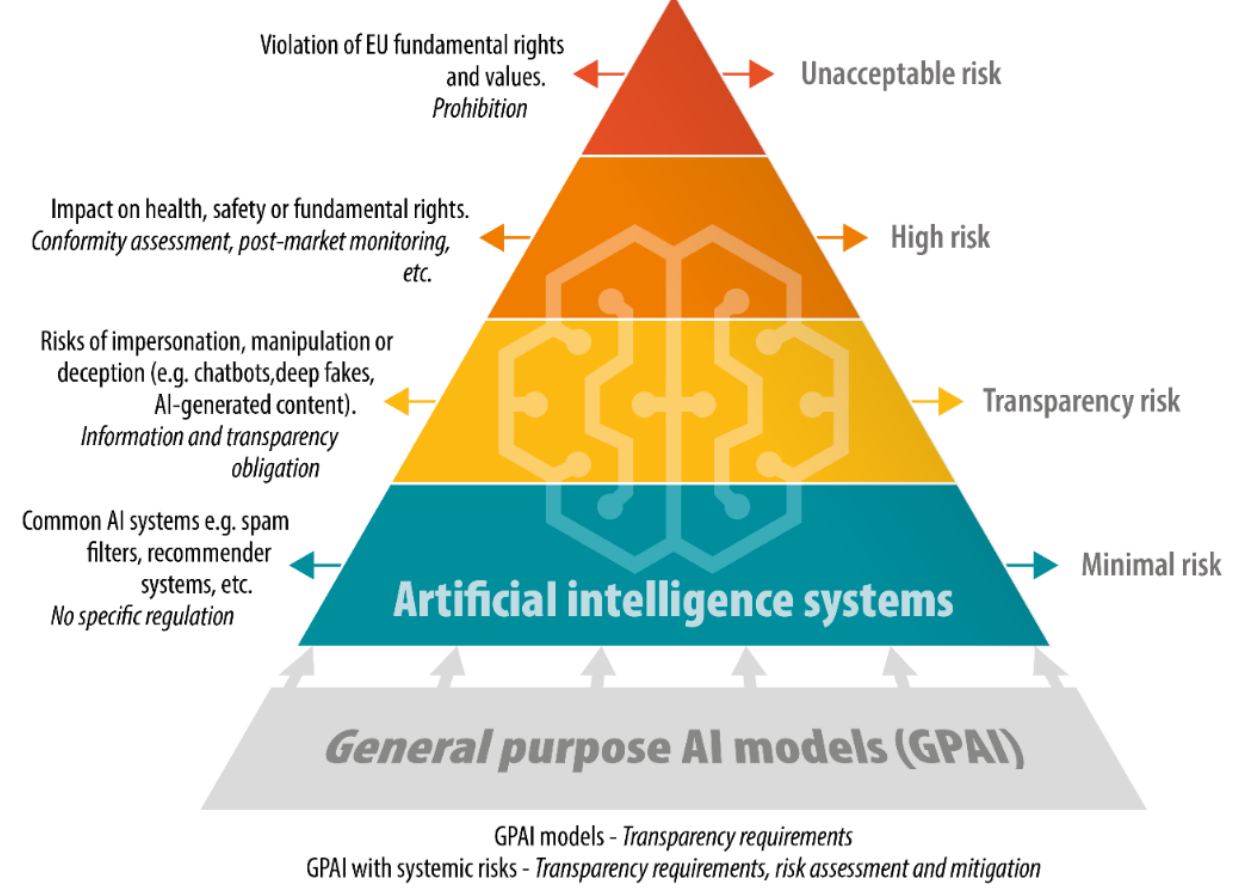
\includegraphics[width=.75\textwidth]{screen2.png}
\caption{Jupyter Notebook}
\label{fig:jupyter}
\end{figure}

The immediate feedback upon code execution helps in quick hypothesis testing and data manipulation. Furthermore, the integration of rich media alongside code makes Jupyter Notebooks an excellent tool for creating comprehensive documentation, tutorials, and educational materials.

Notebooks can be easily shared, making them popular in collaborative projects. The ability to see the code, along with its output and accompanying explanation, in a single document enhances understanding and teamwork. Jupyter Notebooks run in a web browser, offering platform independence and eliminating the need for complex software application setups.

When working with Jupyter Notebooks, the term ''kernel'' denotes a particular version of the Python programming language and environment (i.e. Python packages, etc.) that runs your code. You can enter code in an empty cell and press \colorbox{lightgray}{CTRL-ENTER} to execute code in the cell. A cell can contain multiple lines of code. Jupyter Notebook cells can be merged, split, moved, copied, and deleted, and you can save, import, and export notebooks, among much other, advanced functionality.

\paragraph{PyCharm IDE:} The PyCharm Integrated Development Environment (IDE) is a full-featured software development environment designed specifically for Python. It offers a wide range of tools and features for professional software development, including code completion, debugging, project management, version control integration, and a powerful code editor. PyCharm is more suited for larger and more complex software projects. Its sophisticated environment, while powerful, might be overwhelming for beginners or for those who require a simple platform for exploratory data analysis. Figure~\ref{fig:pycharm} shows a screenshot of the PyCharm IDE.

\begin{figure}
\centering
\includegraphics[width=.75\textwidth]{screen4.png}
\caption{PyCharm Integrated Development Environment (IDE)}
\label{fig:pycharm}
\end{figure}

One of the key strengths of PyCharm is its intelligent code editor, offering features like code completion, code inspections, and automated refactoring. These features greatly enhance productivity and reduce the likelihood of programming errors. Additionally, PyCharm includes an integrated debugger and testing support, simplifying the process of diagnosing and fixing issues in programming code. The IDE also offers seamless integration with version control systems like Git, which is essential for collaborative development and code management.

In summary, while the Interactive Python Shell is best for quick, simple tasks and learning the basics, Jupyter Notebooks are ideal for business analytics projects that benefit from an interactive, explanatory, and exploratory approach. PyCharm is the most suitable for comprehensive software development, offering robust tools and features for managing complex codebases. The choice among these depends largely on the specific requirements of the project and the preferences of the developer.

%\FloatBarrier

\section{Python Basics}

The basic Python code in the following example prints a character string. The \texttt{print} function in Python is very versatile and provides different ways to print the values of multiple variables. In particular, character strings have a \texttt{format} function that can be used to substitute the \texttt{\{\}} placeholders with values, either by index/number, by name, or by position, as shown in the following Python code block that defines two variables, \texttt{age} and \texttt{name} and prints their values in a variety of ways:

\begin{samepage}
\begin{pythoncode}
print('hello world')

age = 19
name = 'Malina'
print('{0} is {1} years old'.format(name, age))
print('{name} is {age} years old'.format(name=name,age=age))
print('{} is {} years old'.format(name, age))
print(f'{name} is {age} years old')
print(name+' is '+str(age)+' years old')
\end{pythoncode}
\end{samepage}

\noindent Because Python commands can get quite long, Python allows for backslashes to break long lines and continue the command on the following line. While not needed in this case, the following code block illustrates how to use them:

\begin{samepage}
\begin{pythoncode}
print('This is a very long \
string and needs a second line')
i = \
5
print(i)
\end{pythoncode}
\end{samepage}

\noindent Multiline character strings are enclosed in triple quotes, and the line breaks form part of the string, as shown in the following example. Note that the \texttt{print(s)} function prints the line breaks in the character string.

\begin{samepage}
\begin{pythoncode}
s = '''This is line 1
and here is line 2
and now this is line 3'''
print(s)
\end{pythoncode}
\end{samepage}

\noindent As with R, you can use Python interactively as a calculator. It provides the usual arithmetic operators and comparison operators The \texttt{//} operator is for integer division with floor (rounding down), the \texttt{\%} operator is the modulus (remainder) operator. Boolean values are \texttt{True} and \texttt{False} in Python and \emph{cannot} be abbreviated (unlike in R). The following Python code block illustrates typical usage:

\begin{samepage}
\begin{pythoncode}
2 + 2
2**4
13 // 3
-13 // 3
13 % 3
-25.5 % 2.25
3 < 5
3 > 5
3 == 5
(3 < 5) and (4 < 2)
(3 < 5) or not (4 < 2)
\end{pythoncode}
\end{samepage}

\noindent The next code example shows some useful string functions. The \texttt{startwith()} function does what its name suggests and returns a boolean (True or False) value. The \texttt{find()} function returns either the first position of a string in another string, or -1 if the string is not found. 
\begin{samepage}
\begin{pythoncode}
language = 'Innuktitut'
if language.startswith('Innu'):
    print('Yes, the string starts with "Innu"')
if 'u' in language:
    print('Yes, it contains the string "u"')
if language.find('nuk') != -1:
    print('Yes, it contains the string "nuk"')
\end{pythoncode}
\end{samepage}

The \texttt{join()} and \texttt{split()} functions for character strings do as the their names suggest and work with Python lists, illustrated in the code block below:

\begin{samepage}
\begin{pythoncode}
# Joining and Splitting    
delimiter = '_*_'
mylist = ['Nain', 'Hopedale', 'Makkovik', 'Rigolet']
mystring = delimiter.join(mylist)
print(mystring)
thelist = mystring.split(delimiter)
print(thelist)
\end{pythoncode}
\end{samepage}

\begin{tcolorbox}[colback=alert]
\paragraph{Important:} Note the use of leading whitespace or indentation in the lines after the \texttt{if} statement in the above code. In Python, this \emph{whitespace is required for defining the program logic}! In the above example, the indented lines indicate the extent of the program block to be executed after the \texttt{if} statement. The normal leading whitespace is four spaces. 
\end{tcolorbox}

\emph{Lists}\index{List} in Python are ordered collections of items, and use square brackets \texttt{[]} as delimiters. Lists are mutable, i.e. their contents can be changed. Lists may contain items of different data types, including other lists or structured data types. Useful list functions are \texttt{len()} which returns the number of items in a list, \texttt{append()}, which adds items to the end of the list, and \texttt{sort()}, which sorts by value (only for compatible data types in the list). Items can be removed by position using the \texttt{del()} or by value using the \texttt{remove()} functions.

\begin{samepage}
\begin{pythoncode}
# Inuit deities
gods = ['Sedna', 'Nanook', 'Akna', 'Pinga']
print('There are', len(gods), 'deities:')
for god in gods:
    print(god, end=' ')

# Appending to a list
gods.append('Amaguq')
print('\nThe list of deities is now', gods)

# Sorting a list
gods.sort()
print('The sorted list is', gods)

# Removing items from a list
print('The first deity is', gods[0])
olditem = gods[0]
del gods[0]
print('I removed', olditem)
print('The list is now', gods)
gods.remove('Pinga')
print('The list is now', gods)
\end{pythoncode}
\end{samepage}

\noindent The above example also shows the use of Python comments, beginning with \texttt{\#} to the end of the line. The example also shows iteration (''repeating'') with the \texttt{for} statement. Similar to the earlier example illustrating the \texttt{if} statement, note the required indentation (leading whitespace) in the line(s) after the \texttt{for} statement to indicate the extent of the code block that is repeated.

\emph{Tuples}\index{Tuple (in Python)} in Phython are also ordered collections of items, but they are immutable, i.e. their contents cannot be changed. Tuples use round brackets \texttt{()} as delimiters.

\begin{samepage}
\begin{pythoncode}
# Inuit Nunangat
regions = ('Inuvialuit', 'Nunavut', 'Nunavik', 'Nunatsiavut')
print('Number of regions is', len(regions))

all_regions = 'NunatuKavummiut', 'Kalaallit', 'Inupiaq', regions
print('Number of all Inuit regions:',len(all_regions))
print('All Inuit regions are', all_regions)
print('Regions in Inuit Nunangat are', all_regions[3])
print('First region in Inuit Nunangat is', all_regions[3][1])
print('Number of all Inuit regions is', \
    len(all_regions)-1+len(all_regions[3]))
\end{pythoncode}
\end{samepage}

\begin{tcolorbox}[colback=alert]
\paragraph*{Important:} Indexing in Python is zero based, that is, the first element in a list or tuple is number 0, while the last element is number \texttt{len()} - 1. This is in contrast to R, where indexing starts at 1.
\end{tcolorbox}

\emph{Dictionaries}\index{Dictionary (in Python)}\index{Dict|see{Dictionary (in Python)}} (or short, ''dicts'') in Python are key-value pairs that map one element to another. In other programming languages, this data structure is also called a \emph{map} or an \emph{associative array}\index{Associative array|see{Dictionary (in Python)}} (because it associates keys with their values). Python uses curly brackets \texttt{\{\}} as delimiters; the keys and values are separated using \texttt{:}. The value for a key is retrieved using the square bracket operator \texttt{[]}. Keys and values may be any data type.

\begin{samepage}
\begin{pythoncode}
# Largest citites
c = {
    'Inuvialuit': 'Inuvik',
    'Nunavut': 'Iqaluit',
    'Nunavik': 'Kuujjuaq',
    'Nunatsiavut': 'Nain' 
}
print("Nunavik's largest city is", c['Nunavik'])
\end{pythoncode}
\end{samepage}

Keys and values can be retrieved separately using the function \texttt{keys()} and \texttt{values()}. Dicts are mutable, as the following example shows by removing an entry with \texttt{del} and adding another entry.

\begin{samepage}
\begin{pythoncode}
# Retrieving keys and values
print(list(c.keys()))
print(list(c.values()))

# Deleting a key-value pair
del c['Nunavut']
print('\nThere are {} cities left\n'.format(len(c)))
for region, city in c.items():
    print('{} is largest city of {}'.format(city, region))

# Adding a key-value pair
c['Nunavut'] = 'Iqaluit'
if 'Nunavut' in c:
    print("\nNunavut's largest city is", c['Nunavut'])
\end{pythoncode}
\end{samepage}

A useful function to create dicts from two lists is the \texttt{zip()} function, shown below. The \texttt{zip()} function creates an iterator over fixed-length tuples that are passed into the dictionary creation function \texttt{dict()} as key--value tuples:

\begin{samepage}
\begin{pythoncode}
towns = ['Hopedale', 'Makkovik', 'Nain', 'Postville', 'Rigolet']
pops = [596, 365, 1204, 188, 327]
pop_by_town = dict(zip(towns, pops))
print(pop_by_town)
\end{pythoncode}
\end{samepage}

In Python, lists, tuples, and character strings are examples of \emph{sequences}\index{Sequence (in Python)}. All sequences provide membership tests using \texttt{in} or \texttt{not in} operators, as shown in some of the examples above. Sequences also provide integer indexing and slicing.  Note that the end index in a slicing expression is \emph{not inclusive}, that is, the slice extends up to but does not include the final index. This makes it easy to write a slice like \texttt{[:len(a)]} where \texttt{a} is some sequence (rather than having to write \texttt{[:len(a)-1]} as one would in R or other programming languages where the end index is inclusive).

The following code shows some examples for slicing\index{Slicing} tuples. Note the negative end index in the third example. A negative end index iterates from the end of a sequence forwards''. The slice \texttt{regions[1:-1]} extends from the second element to the third of the four elements. 

\begin{samepage}
\begin{pythoncode}
regions = ('Inuvialuit', 'Nunavut', 
           'Nunavik', 'Nunatsiavut')
# Slicing on a tuple
print('Item 1 to 3 is', regions[1:3])
print('Item 2 to end is', regions[2:])
print('Item 1 to -1 is', regions[1:-1])
print('Item start to end is', regions[:])
\end{pythoncode}
\end{samepage}

Slicing in Python is more advanced than slicing in R as not only the beginning and end index can be specified, but also the step size, as shown in the next Python code block. The final example slices backwards.

\begin{samepage}
\begin{pythoncode}
# Slicing with step
print(regions[::1])
print(regions[::2])
print(regions[::3])
print(regions[::-1])
\end{pythoncode}
\end{samepage}

Character strings are also sequences, and they support slicing or indexing the same way as other sequences in Python.

\begin{samepage}
\begin{pythoncode}
language = 'Innuktitut'
# Slicing on a string 
print('characters 1 to 3 is', language[1:3])
print('characters 2 to end is', language[2:])
print('characters 1 to -1 is', language[1:-1])
print('characters start to end is', language[:])
\end{pythoncode}
\end{samepage}

\noindent In the above example, pay careful attention to the use of negative indices in the slicing expressions, both for the index as well as the step size.

\begin{tcolorbox}[colback=code]
\paragraph*{Tip:} To read and execute Python statements from a file, use the expression \texttt{exec(open('filename.py').read())}
\end{tcolorbox}

\begin{tcolorbox}[colback=code]
\subsubsection*{Hands-On Exercise}
\begin{enumerate}
    \item Create a \emph{list} containing the numbers 1 to 10. Use list slicing to create a sublist with only the even numbers.
    \item Using a \texttt{for} loop, sum all the items in the list.
    \item Using a \texttt{for} loop, iterate over the list and print each number squared.
    \item Write a program to append the square of each number in the range [1:5] to a new list.
\end{enumerate}
\end{tcolorbox}

\begin{tcolorbox}[colback=code]
\subsubsection*{Hands-On Exercise}
\begin{enumerate}
    \item Create a \emph{tuple} with different data types (string, int, float).
    \item Demonstrate how tuples are immutable by attempting to change its first element.
    \item Write a program to convert the tuple into a list.
\end{enumerate}
\end{tcolorbox}

\begin{tcolorbox}[colback=code]
\subsubsection*{Hands-On Exercise}
\begin{enumerate}
    \item Create a \emph{dictionary} with at least three key-value pairs, where the keys are strings and the values are numbers.
    \item Write a Python script to add a new key-value pair to the dictionary and then print the updated dictionary.
    \item Create a nested dictionary, that is, a dictionary whose values are dictionaries, and demonstrate accessing elements at various levels.
\end{enumerate}
\end{tcolorbox}

\section{NumPy}

NumPy, short for Numerical Python, is an essential package for the Python programming language, widely used for scientific computing and data analysis. It provides powerful numerical arrays and matrices, along with a large collection of high-level mathematical functions to operate on these arrays. The cornerstone of NumPy is its ''ndarray'' (n-dimensional array)\index{Array (in Python)} object. These arrays are more efficient than Python's built-in lists, especially for numerical operations, due to their fixed type and contiguous memory allocation.

NumPy arrays facilitate advanced mathematical and statistical operations, including linear algebra, Fourier transform, and random number generation. The ndarray object supports vectorized operations, broadcasting, and indexing capabilities. This means that operations can be applied to entire arrays without the need for explicit loops, leading to cleaner and faster code.

One of the reasons for NumPy's popularity in the scientific and data science communities is its seamless integration with other Python libraries. Libraries like Pandas for data manipulation and analysis, Matplotlib for data visualization, and SciPy for scientific computing all build upon and work in conjunction with NumPy, creating a robust ecosystem for scientific computing tasks.

\begin{tcolorbox}[colback=code]
\paragraph*{Tip:} The NumPy website provides two very good introductions, in the form of the \href{https://numpy.org/doc/stable/user/quickstart.html}{Quick Start} and the \href{
https://numpy.org/doc/stable/user/absolute_beginners.html}{NumPy for absolute beginners} tutorials.
\end{tcolorbox}

NumPy ndarrays have a set of useful properties or attributes, summarized in in Table~\ref{tab:numpydatatypes}. Note that the terminology is \emph{''axes''}, rather than \emph{''dimensions''} as in the previous chapter on R, although the \texttt{ndim} property of an ndarray uses the term ''dimension'' in its name.

\begin{table}
\centering
\renewcommand{\arraystretch}{1.25}
\begin{tabularx}{\linewidth}{l|X} \hline
\texttt{ndarray.ndim} & Number of axes \\
\texttt{ndarray.shape} & Typle describing the size of each axis (dimension)\index{Shape (of array)} \\
\texttt{ndarray.size} & Total number of elements \\
\texttt{ndarray.dtype} & The datatype of the elements, for example \texttt{numpy.int32}, \texttt{numpy.int16}, \texttt{numpy.float32}, or \texttt{numpy.float64} \\
\texttt{ndarray.itemsize} & Number of bytes for each element \\ \hline
\end{tabularx}
\caption{Attributes of NumPy ndarray}
\label{tab:numpydatatypes}
\end{table}

The following Python code block illustrates the use of these properties. Note the use of the \texttt{arange()} function to create a one-dimensional array of 15 numbers (from 0 to 14), that is then \texttt{reshape}d into a 2-dimensional array with 3 rows and 5 columns. Rows are axis 0, and columns are axis 1.

\begin{samepage}
\begin{pythoncode}
# Import the numpy package
import numpy as np

# Create an array
a = np.arange(15).reshape(3, 5)

print(a.shape)
print(a.ndim)
print(a.dtype.name)
print(a.size)
print(type(a))
\end{pythoncode}
\end{samepage}

The following Python code block shows element-wise operations and array operations on a NumPy array. Python determines automatically which functions are array functions (like \texttt{sum()}) and which ones are element-wise functions (like \texttt{sqrt()}). Note the creation of the array with the \texttt{array()} function from a list of two tuples. Note also the use of the \texttt{axis} pararmeter in the \texttt{max} function to specify whether to aggregate by row or by column. The \texttt{axis} parameter can also be applied to other functions like \texttt{sum()} or \texttt{std()}.

\begin{samepage}
\begin{pythoncode}
# Create an array from Python lists and tuples
b = np.array([(1.5, 2., 3), (4, 5, 6)])

# Elementwise operations
print(3 * b)
print(b + 5)
print(np.sqrt(b))

# Array operations
print(np.max(b))
print(np.max(b, axis=0))
print(np.max(b, axis=1))
print(np.std(b))
print(np.cov(b))
print(np.sum(b))
\end{pythoncode}
\end{samepage}

In the above example, the \texttt{std()} function without \texttt{axis} parameter computes the standard deviation of all elements in the array, while \texttt{cov} treats each \emph{row} of the array as a vector and computes their variances and covariances. To treat array columns as vectors, either transpose the array first, using the \texttt{T} operator or use the \texttt{rowvar=False} parameter for the \texttt{cov()} function. 

To create pre-initialized arrays, NumPy provides two convenience functions to create arrays filled with 0s or 1s:
\begin{samepage}
\begin{pythoncode}
# Create an array of zeros with shape (3,4)
x = np.zeros((3,4))
print(x)

# Create an array of ones with shape (2,3,4)
y = np.ones((2,3,4))
print(y)
\end{pythoncode}
\end{samepage}

In a generalization of the slicing expressions for Python sequences, each axis of a NumPy array can be sliced using the \texttt{[:]} or \texttt{[::]} expressions, as shown in the following example of a two-dimensional array\index{Slicing}. The slicing expressions for different dimensions are separated by commas.

\begin{samepage}
\begin{pythoncode}
b = np.array([[ 0,  1,  2,  3],
              [10, 11, 12, 13],
              [20, 21, 22, 23],
              [30, 31, 32, 33],
              [40, 41, 42, 43]])
print(b[2, 3])
print(b[0:5, 1])
print(b[:, 1])
print(b[1:3, :])
print(b[-1])
\end{pythoncode}
\end{samepage}

When not all axes are supposed to be sliced, one can omit initial or final unsliced axes in the slicing expression using the ellipsis ''...'' as shown in the following Python code block.

\begin{samepage}
\begin{pythoncode}
c = np.array([[[  0,  1,  2],
               [ 10, 12, 13]],
              [[100, 101, 102],
               [110, 112, 113]]])
print(c[1, ...])
print(c[1, : , : ])
print(c[..., 2])
print(c[: , : , 2])
print(c[..., : , 1])
\end{pythoncode}
\end{samepage}

NumPy arrays also provide convenient iteration of their rows and their elements. Note the use of the \texttt{flat} operator to ''flatten'' a multi-dimensional array to a single dimension in the code block below.

\begin{samepage}
\begin{pythoncode}
for row in b:
    print(row)

for element in b.flat:
    print(element)
\end{pythoncode}
\end{samepage}

NumPy provides an easy way to reshape arrays to any dimension. However, it is important to be aware of where and how the elements move during such a reshape. The order can be specified using an optional argument to \texttt{rehshape}; consult the NumPy documentation for details. The following example also demonstrates the use of the default random number generator\footnote{A random number generator in computer science is always a pseudo-random number generator that creates a sequence of numbers according to a deterministic formula (because computers are deterministic), starting from an initial ''seed'' number. The sequence is repeatable when beginning with the same seed. A good pseudo-random number generate will create sequences that are indistinguishable from true random numbers, for example, those created by rolling dice.} (rng)\index{Random number generator} in NumPy to create an array of shape \texttt{(3, 4)} filled with random numbers between 0 and 1.

\begin{samepage}
\begin{pythoncode}
# Create a random number generator with seed 1
rg = np.random.default_rng(1)

# Create an array of shape (3, 4) of random numbers
a = np.floor(10 * rg.random((3, 4)))

# Show information about the array and reshape
print(a.shape)
print(a.flatten())
print(a.reshape(6, 2))
print(a.T)
print(a.T.shape)
\end{pythoncode}
\end{samepage}

The above example uses the \texttt{flatten()} function which returns a one-dimensional array, whereas the \texttt{flat} property returns an iterator to be used in a \texttt{for} loop. The \texttt{T} property returns the transpose of the array. In two dimensions, the transpose swaps rows and columns. The NumPy transpose is also defined for more than two dimensions, the axes are transposed such that \texttt{a.T.shape==a.shape[::-1]}.

The next example illustrates concatenation or stacking operations to stack two arrays either vertically, that is, by row, or horizontally, that is, by column. The arrays must be of compatible shape for these stacking operations. 

\begin{samepage}
\begin{pythoncode}
b = np.floor(5 * rg.random((3, 4)))
print(np.vstack((a, b)))
print(np.hstack((b, a)))
\end{pythoncode}
\end{samepage}

Arrays can be indexed also by boolean arrays. For example, in the following Python code block, the expression \texttt{a < 5} constructs a boolean array whose entries are \texttt{True} when the corresponding element in \texttt{a} is less than 5. This boolean array is then used to select or index the array \texttt{a}:

\begin{samepage}
\begin{pythoncode}
a = np.array([[1, 2, 3, 4], 
              [5, 6, 7, 8], 
              [9, 10, 11, 12]])
print(a[a < 5])
print(a < 5)
print(a[a%2 == 0])
print(a%2 == 0)
\end{pythoncode}
\end{samepage}

Finally, NumPy provides easy ways to identify unique elements in an array and to count how often particular elements occur in an array. The following example also demonstrates another use of the \texttt{zip()} function, already introduced above, to construct a list of tuples.

\begin{samepage}
\begin{pythoncode}
a = np.array([11, 11, 12, 13, 14, 15, 16, 
              17, 12, 13, 11, 14, 18, 19, 20])
print(np.unique(a))

# Return the first index of a unique value
values, indices = np.unique(a, return_index=True)
print(list(zip(values, indices)))

# Return the counts of each unique value
values, counts = np.unique(a, return_counts=True)
print(list(zip(values, counts)))
\end{pythoncode}
\end{samepage}

\begin{tcolorbox}[colback=code]
\subsubsection*{Hands-On Exercises}
\begin{enumerate}
   \item Create an array with random numbers in the shape indicated by the last four digits of your student number (if your student number contains a 0, use a 1 instead)
   \item Construct a new array by swapping the first half of rows (axis 0) with the second half of rows (axis 0)
   \item Calculate all covariance matrices formed by the last two axes of your array. \emph{Tip:} Iterate over the first two axes/dimensions with a \texttt{for} loop
   \item Subtract the mean of the array from each element in the array (mean normalization)
   \item Select all elements that are greater than the overall mean
   \item Sort the selected elements from the previous step
\end{enumerate}
\end{tcolorbox}

\section{Data management with Pandas}

Pandas is a Python package widely used in data science, data analysis, and machine learning. It is known for its powerful data manipulation and analysis capabilities. It provides fast, flexible, and expressive data structures designed to make working with structured (tabular, multidimensional, potentially heterogeneous) and time series data both easy and intuitive. 

Pandas is useful for data cleaning, data transformation, and data analysis. It offers functions for reading and writing data in various formats such as CSV, Excel, JSON, and SQL databases. The Pandas package simplifies handling missing data, merging and joining datasets, reshaping, pivoting, slicing, indexing, and subsetting data. Its time series functionality is particularly robust, offering capabilities for date range generation, frequency conversion, moving window statistics, date shifting, and lagging.

The library's design and functionality are heavily influenced by data analysis needs in finance, which is evident in its powerful group-by functionality for aggregating and transforming datasets, as well as its high-performance merging and joining of datasets. As part of the broader Python scientific computing ecosystem, which includes libraries like NumPy, Matplotlib, and Scikit-learn, Pandas plays an important role in data analysis and machine learning workflows.

\begin{tcolorbox}[colback=code]
\paragraph*{Tip:}
The Pandas website provides very good \href{http://pandas.pydata.org/docs/user_guide/10min.html}{10 Minutes to Pandas} introductory tutorial for Pandas.
\end{tcolorbox}

Central to Pandas are two primary data structures: the DataFrame and the Series. A Series in Pandas is a one-dimensional array-like object that can hold any data type, including integers, floats, strings, and Python objects. A DataFrame in Pandas is a two-dimensional, size-mutable, and potentially heterogeneous tabular data structure with labeled axes (rows and columns).

The following Python code constructs a Pandas Series of random numbers\index{Series (in Pandas)}. The axis labels of a Series (and a DataFrame) are called ''index'' and allow one to name the elements. The example also shows how a Python dict can be converted into a series with named elements.

\begin{samepage}
\begin{pythoncode}
# Import the Pandas package
import pandas as pd

# Create a series from a NumPy array of random numbers
s = pd.Series(np.random.randn(5))
print(s.index)

# Provide indices (labels) when creating the series
s = pd.Series(np.random.randn(5), index=["a", "b", "c", "d", "e"])
print(s.index)

# Create a series from a Python dict that provides labels and values
d = {"a": 0.0, "b": 1.0, "c": 2.0}
print(pd.Series(d))

# Create a series from a dict and reorder the entries
print(pd.Series(d, index=["b", "c", "d", "a"]))
\end{pythoncode}
\end{samepage}

Note that in the last line of the above example, renaming or reordering the elements of the Series \texttt{d} introduces a \texttt{NaN} element for the index ''d'', because the dict contains no value for the key ''d''.

Pandas series behave largely like NumPy arrays, but note that to access their elements by numerical index, one has to use the \texttt{iloc} operator, as shown in the following Python code block. This allows slicing the same way as for Python sequences or NumPy arrays. The following example also shows that Series can behave like a Python dict, in that values for a named index (''key'') can be retrieved. Series also provide membership tests for ''keys'' using \texttt{in}. 

\begin{samepage}
\begin{pythoncode}
# Series behave like an ndarray
print(s.iloc[0])
print(s.iloc[:3])
print(s[s > s.median()])
print(s.iloc[[4, 3, 1]])
print(np.exp(s))

# Series behave like a dict
print(s['a'])
print(s['e'])
print('e' in s)
print('f' in s)

# Series have a datatype and name
s.name = 'My First Series'
print(s.dtype)
\end{pythoncode}
\end{samepage}

Pandas \emph{DataFrames} are two-dimensional objects\index{Data frame!in Pandas}. Their columns may have different data types. Conceptually, DataFrames can be considered as a dict of Pandas Series, as the following example demonstrates. 

\begin{samepage}
\begin{pythoncode}
d = {
    "one": pd.Series([1.0, 2.0, 3.0], 
                index=['a', 'b', 'c']),
    "two": pd.Series([1.0, 2.0, 3.0, 4.0], 
                index=['a', 'b', 'c', 'd'])
}
df = pd.DataFrame(d)
print(df)
print(df.index)
print(df.columns)
print(pd.DataFrame(d, index=['d', 'b', 'a'], 
                      columns=['two', 'three']))
\end{pythoncode}
\end{samepage}

Constructing the DataFrame \texttt{df} ''lines up'' the two Series on their common indices, and will introduce a ''NaN'' for index ''d'' in column ''one'', because that Series does not contain a value for ''d''. Similarly, inserting a column named ''three'' in the last line of the above example yields a column filled with ''NaN'' because the dict \texttt{d} does not contain values for the key ''three''.

DataFrame columns can be accessed using their quoted name, and will yield a Pandas Series with the usual operations. The following Python code example shows that new columns can be added simply by defining them, as in the ''flag'' column below or using the \texttt{assign()} function, which works similarly to the \texttt{mutate} function in R/dplyr. Columns can be removed using the \texttt{del} command or the \texttt{pop()} function. The latter returns the deleted column as a Series.

\begin{samepage}
\begin{pythoncode}
print(df['one'])
df['three'] = df['one'] * df['two']
df['flag'] = df['one'] > 2
print(df)

del df['two']
three = df.pop('three')
df['foo'] = 'bar'
df['one_trunc'] = df['one'][:2]
df.insert(1, 'bar', df['one'])
print(df)

# Similar to 'mutate' in R/Dplyr 
df = df.assign(four = df['one'] * np.sqrt(df['bar']))
print(df)
\end{pythoncode}
\end{samepage}

Pandas DataFrames can be index by colum, by label, by integer location, or by boolean vectors. Table\ref{tab:pandasindexing} shows an overview of the different methods and their return values.

\begin{table}[h]
\centering
\renewcommand{\arraystretch}{1.25}
\begin{tabular}{l|l|l} \hline
Select column & \texttt{df['colname']} & Series \\
Select row by label & \texttt{df.loc['label']}  & Series \\
Select row by integer location & \texttt{df.iloc[loc]} & Series \\
Slice rows & \texttt{df[::]} & DataFrame \\
Select rows by boolean vector & \texttt{df[bool]} & DataFrame \\ \hline
\end{tabular}
\caption{Methods for indexing Pandas DataFrames}
\label{tab:pandasindexing}
\end{table}

As noted earlier, Pandas automatically aligns data by indices, that is, by row and column labels, for operations on dataframes. Note how the addition of two dataframes of unequal shape introduces ''NaNs''. For convenience, NumPy operations can also be used to operate on Pandas DataFrames, which are automatically converted to NumPy ndarrays before and converted back after such an operation. 

\begin{samepage}
\begin{pythoncode}
df = pd.DataFrame(np.random.randn(10, 4), 
                  columns=["A", "B", "C", "D"])
df2 = pd.DataFrame(np.random.randn(7, 3), 
                   columns=["A", "B", "C"])
print(df + df2)

# Elementwise operators
print(df * 5 + 2)
print(1/df)
print(df**4)

# Transpose
print(df.T)

# Using Numpy functions
print(np.exp(df))
print(np.asarray(df))
\end{pythoncode}
\end{samepage}

To apply element-wise character string operations on Series or DataFrames it is useful to use the \texttt{str} property:

\begin{samepage}
\begin{pythoncode}
# String functions with 'str'
s = pd.Series(
    ["A", "B", "C", "Aaba", "Baca", np.nan, 
     "CABA", "dog", "cat"], dtype="string")
s.str.lower()
\end{pythoncode}
\end{samepage}

Pandas provides a number of useful functions to get information about the contents of a DataFrame. The \texttt{info()} function provides information about the columns and their data types, while \texttt{head()} and \texttt{tail()} print the first and last few lines of a DataFrame. 

\begin{samepage}
\begin{pythoncode}
df.info()
df.head()
df.tail(3)
\end{pythoncode}
\end{samepage}

The \emph{boolean reduction} functions \texttt{all()} and \texttt{any()} operate by column on DataFrames with boolean values. As their names suggest, \texttt{all()} returns \texttt{True} when the all entries in a column are true, whereas \texttt{any()} returns \texttt{True} if any of the entries in a column are true. The last line of the following Python code block re-applies \texttt{any()} to the Series that results from the first application of \texttt{any()}.

\begin{samepage}
\begin{pythoncode}
# Boolean reductions
(df > 0).all()
(df > 0).any()
(df > 0).any().any()
\end{pythoncode}
\end{samepage}

When making comparisons on DataFrames that include ''NaN'', it is important to realize that two ''NaNs'' are not equal when using the \texttt{==} operator, but they are equal when using the \texttt{equals} function. The following example illustrates this difference.

\begin{samepage}
\begin{pythoncode}
# NaN's are not the same
df.iloc[0,0] = np.nan
(df+df == df*2).all()
(df + df).equals(df*2)
\end{pythoncode}
\end{samepage}

Pandas provides useful functions for basic descriptive statistics and aggregation on DataFrames. In particular, the \texttt{describe()} function is useful to get a basic information on the data in a DataFrame. The \texttt{mean()} function takes as its optional first argument the axis number (0 for rows, 1 for columns) and can skip missing values when summing. Multiple aggregates can be formed using the \texttt{agg()} function. The Python code block below illustrates the use of these functions.

\begin{samepage}
\begin{pythoncode}
# Descriptive statistics
df.mean(0)
df.mean(1, skipna=False)
df_std = (df - df.mean()) / df.std()
df.describe()

# Aggregation with 'agg'
df.agg(['sum', 'mean', 'std'], 0)
\end{pythoncode}
\end{samepage}

Pandas DataFrames can be sorted by columns, and the functions \texttt{nlargest()} and \texttt{nsmallest()} can be used to select a DataFrame with only the n smallest or largest values in a given column.

\begin{samepage}
\begin{pythoncode}
# Sort by values
df.sort_values(by=['A', 'B'])
df.nsmallest(3, 'A')
df.nlargest(3, 'A')
\end{pythoncode}
\end{samepage}

A very useful way to identify or select data in a Pandas DataFrame is the \texttt{query()} function, which accepts a simplified boolean condition as argument. This allows one to write much shorter and compact selection logic, as shown in the following example. Note the two different forms of the same logical operator \texttt{\&} and \texttt{and}.

\begin{samepage}
\begin{pythoncode}
df = pd.DataFrame(np.random.rand(10, 3), 
                  columns=list('abc'))

# Pure python
df[(df['a'] < df['b']) & (df['b'] < df['c'])]

# Shorter with Query
df.query('(a < b) & (b < c)')
df.query('a < b & b < c')
df.query('a < b and b < c')
df.query('a < b < c')
\end{pythoncode}
\end{samepage}

The \texttt{query()} function can also be used for membership tests in Series and DataFrames using the \texttt{in} operator. This also is much more compact and easy to read than the pure Python \texttt{isin()} function. The following example code block shows the pure Python selection followed by equivalent selection with \texttt{query()}:

\begin{pythoncode}
df = pd.DataFrame({'a': list('aabbccddeeff'), 
                   'b': list('aaaabbbbcccc'),
                   'c': np.random.randint(5, size=12),
                   'd': np.random.randint(9, size=12)})      
                   
# Pure Python versus Query
df[df['a'].isin(df['b'])]  
df.query('a in b')  

df[~df['a'].isin(df['b'])] 
df.query('a not in b')     

df[df['b'].isin(df['a']) & (df['c'] < df['d'])]          
df.query('a in b and c < d') 

df[df['b'].isin(["a", "b", "c"])]
df.query('b == ["a", "b", "c"]')    

df[df['c'].isin([1, 2])]
df.query('[1, 2] in c')      
\end{pythoncode}

Pandas DataFrames also offer easy functions to remove duplicates. The following Python example code block shows how to identify rows that contain duplicate elements in a list of columns, and then remove the duplicates, keeping either the first or the last row. Note the different row indices in the retained results of \texttt{drop\_duplicates} and their different values columns ''c'' and ''d''.

\begin{pythoncode}
df2 = df.copy()

df2.duplicated(['a', 'b'])
df2.drop_duplicates(['a', 'b'], keep='last')
df2.drop_duplicates(['a', 'b'], keep='first')
\end{pythoncode}

Finally, Pandas provides many functions for reading and writing DataFrames from and to a variety or serialization formats and even SQL RDBMS. See the \href{https://pandas.pydata.org/docs/user_guide/io.html#}{Pandas IO user guide} for details. 

\section{The Pagila Database in Pandas}

This section the use of Pandas for descriptive data analysis using the Pagila database data as an example. The Pagila database\footnote{\url{https://github.com/devrimgunduz/pagila}, \\
\url{https://github.com/devrimgunduz/pagila/blob/master/LICENSE.txt}} is a demonstration database originally developed for teaching and development of the MySQL RDBMS under the name Sakila\footnote{\url{https://dev.mysql.com/doc/sakila/en/}, \\
\url{https://dev.mysql.com/doc/sakila/en/sakila-license.html}}. Pagila is designed as a sample database to illustrate database concepts and is based on a fictional DVD rental store. It originally consists of several tables organized into categories like film and actor information, customer data, store inventory, and rental transactions. For this chapter, the Pagila data was summarized in a few related CSV files. 

The following Python code block reads the rentals data of the Pagila database into a Pandas DataFrame using the \texttt{read\_csv()} function. It then converts the data type of some columns from character strings to datetime types so that one can use date and time operations and arithmetic later.

\begin{samepage}
\begin{pythoncode}
# Read CSV
rentals = pd.read_csv('rentals.csv')

# Convert data types
rentals['rental_date'] = \
    pd.to_datetime(rentals['rental_date'], utc=True)
rentals['return_date'] = \
    pd.to_datetime(rentals['return_date'], utc=True)
rentals['payment_date'] = \
    pd.to_datetime(rentals['payment_date'], utc=True)

# Basic information
rentals.info()
rentals.describe()
rentals.index
rentals.columns
rentals.shape
\end{pythoncode}
\end{samepage}

When working with data, it is often useful to first identify and remove missing values. The following Python code block first identifies columns (\texttt{axis=1}) in the dataset that contain any (\texttt{any()}) missing values (\texttt{isna()}). Of these filtered rentals, only some columns are selected.

\begin{samepage}
\begin{pythoncode}
filtered_rentals = rentals[rentals.isna().any(axis=1)]

selected_rentals = \
    filtered_rentals[
      ['last_name', 'rental_date', 'return_date', 'title', 'amount']]
\end{pythoncode}
\end{samepage}

\noindent When printing DataFrames, Pandas by default abbreviates the output to manageable size. The number of rows and number of columns to be printed is controlled by two Pandas options that can be set as shown in the following example, which removes any limits.

\begin{samepage}
\begin{pythoncode}
pd.set_option('display.max_rows', None)
pd.set_option('display.width', None)
\end{pythoncode}
\end{samepage}

The remainder of this section shows how Pandas can be used to provide equivalent results as obtained in the previous chapter using R/dplyr and in the chapter on relational databases with SQL. \emph{Compare the Python code to the R code and the SQL code to achieve similar results.}

\paragraph*{Example:} Find all films and the actors that appeared in them, ordered by film category and year, for those films that are rated PG.

\begin{samepage}
\begin{pythoncode}
actors = pd.read_csv('actors.categories.csv')

result = pd.merge(rentals, actors, on='title', 
             suffixes=('_customer', '_actor'), how='outer')

result = result[result['rating'] == 'PG']
result['actor'] = result['last_name_actor'] + \
                   ', ' + result['first_name_actor']
          
result.rename(columns={'release_year': 'year'}, inplace=True)

result = result[['actor', 'title', 'category', 'year']]

result.drop_duplicates(['actor', 'title', 'category', 'year'], 
          inplace=True)
          
result.sort_values(['category', 'year', 'title'], inplace=True)

grouped = result.groupby(['category', 'year', 'title'])

g_result = grouped['actor'].apply(list).reset_index()

print(g_result)
\end{pythoncode}
\end{samepage}

This Python code block above performs a series of data manipulation operations using Pandas. The operations merge, filter, transform, and group data from the Pagila movie rental dataset.

\begin{itemize}
\item \emph{Reading Data}: The code reads a CSV file named 'actors.categories.csv' into a DataFrame called ''actors''.
\item \emph{Merging DataFrames}: It then merges two DataFrames: ''rentals'' and ''actors'', based on the ''title'' column that is common to both DataFrames. The \texttt{suffixes} parameter is used to differentiate columns with the same name in both DataFrames, by adding either ''\_customer'' or ''\_actor'' to the column names. The \texttt{how='outer'} parameter ensures that all records from both DataFrames are included in the result, even if there are no matching titles in one of them.
\item \emph{Filtering Data}: After merging, the script filters the resulting DataFrame to include only rows where the ''rating'' column contains the value ''PG''.
\item \emph{Creating a New Column}: A new column, ''actor'', is created by concatenating the ''last\_name\_actor'' and ''first\_name\_actor'' columns, separated by a comma.
\item \emph{Renaming a Column}: The ''release\_year'' column is renamed to ''year''.
\item \emph{Selecting and Rearranging Columns}: The DataFrame is then reduced and rearranged to include only the columns ''actor'', ''title'', ''category'', and ''year''.
\item \emph{Dropping Duplicates}: Duplicate rows based on the combination of ''actor'', ''title'', ''category'', and ''year'' are removed. This ensures that each combination is unique in the dataset.
\item \emph{Sorting Data}: The DataFrame is sorted by ''category'', then ''year'', and finally ''title''.
\item \emph{Grouping Data and Creating a List}: The data is grouped by ''category'', ''year'', and ''title''. For each group, the ''actor'' values are aggregated into a list. This creates a list of actors for each movie title, categorized by year and category.
\item \emph{Resetting Index}: After the grouping and aggregation, the index is reset to turn the grouped data back into a regular DataFrame.
\item \emph{Printing the Final Result}: Finally, the processed DataFrame is printed.
\end{itemize}


\paragraph*{Example:} Find the most popular actors in the rentals in each city.

The Python code block below combines the data frames from the multiple CSV files that make up the Pagila data set, because the combined, full data is used for other analysis examples below.
\begin{itemize} 
\item The Python code merges the ''rentals'' DataFrame with the ''addresses'' DataFrame based on the columns ''customer\_address'' in ''rentals'' and ''address\_id'' in ''addresses'' to linking rentals with corresponding customer addresses.
\item The script then merges the resulting DataFrame with the ''actors'', based on the ''title'' column. 
\end{itemize}

\begin{samepage}
\begin{pythoncode}
addresses = pd.read_csv('addresses.csv')
addresses['phone'] = addresses['phone'].astype(str)

full_data = pd.merge(rentals, addresses, 
                     left_on='customer_address', 
                     right_on='address_id')
                 
full_data = pd.merge(full_data, actors, on='title', 
                     suffixes=('_customer', '_actor'))
\end{pythoncode}
\end{samepage}

The following Python code block performs the required analysis to on the full data constructed above, using the following steps:

\begin{itemize}
\item The code groups the data by ''city'' and ''actor'' and calculates the size of each group. This results in a count of how many times each actor's movies were rented in each city. The result is reset into a DataFrame ''grouped'' with a new column ''count'' representing these sizes.
\item Within each city, actors are ranked based on the ''count'' column, with the ranking stored in a new column ''ranking''. The \texttt{rank} method is set to \texttt{'min'}, which means actors with the same count will have the same rank, and it ranks in descending order of count.
\item The code filters the DataFrame to select the top 3 actors (or ties) in terms of rental counts in each city.
\item The filtered data is then sorted by ''city'', ''ranking'', and ''actor'' before being printed.
\end{itemize}

\begin{samepage}
\begin{pythoncode}
full_data['actor'] = full_data['last_name_actor'] + ', ' + \
                     full_data['first_name_actor']

grouped = full_data.groupby(['city', 'actor']).size() \
            .reset_index(name='count')
            
grouped['ranking'] = grouped.groupby('city')['count'] \
            .rank(method='min', ascending=False)
            
filtered = grouped[grouped['ranking'] < 4]

sorted_df = filtered.sort_values(by=['city', 'ranking', 'actor'])

print(sorted_df)
\end{pythoncode}
\end{samepage}

\paragraph*{Example:} Find the customers who spend the most on rentals, and the number of rentals with the highest total rental payments for each category grouped by rental duration.

\begin{samepage}
\begin{pythoncode}
full_data['customer'] = full_data['first_name_customer'] + ' ' + \
                        full_data['last_name_customer']

selected_data = full_data[['customer', 'amount', 'rental_duration', \
                           'category', 'phone', 'city']]

grouped_data = selected_data \
    .groupby(['category', 'rental_duration', 'customer']) \
    .agg(payments=('amount', 'sum'), num_rentals=('amount', 'count')) \
    .reset_index()
     
grouped_data['ranking'] = grouped_data \
      .groupby(['category', 'rental_duration'])['payments'] \
      .rank(method='min', ascending=False)

top_entries = grouped_data.loc[
    grouped_data.groupby(['category', 'rental_duration'])['ranking'] \
                .idxmin() ]

print(top_entries)
\end{pythoncode}
\end{samepage}

By now, it should be clear what most of the functions in the analysis accomplish. However, two important new things to note. First, the \texttt{agg()} function computes aggregates of the values in its first argument using the function in its second argument and stores the aggregate values in a new column. For example, the code below creates a new column ''payments'' with the ''sum'' of the values of the ''amount'' column of the grouped data, and a new column ''num\_rentals'' with the ''count'' of the values of the ''amount'' column. Second, the \texttt{idxmin()} function within the \texttt{loc[]} operator of the dataframe selects the smallest index, i.e. the smallest (highest) ranking when the data is grouped by category and rental duration.

\paragraph*{Example:} Get the top 5 and the bottom 5 grossing customers for each quarter.

This example demonstrates the Pandas date and time function \texttt{to\_period()}. The argument \texttt{Q} returns quarters. Other frequently used arguments are 'D' for days, 'W' for weeks, 'M' for months, 'Y' for years, 'H' for hours, and 'T' for minutes. The use of the \texttt{sort\_values()} function demonstrates ''mixed'' sorting, ascending by quarter, and descending by payments.

\begin{samepage}
\begin{pythoncode}
full_data['customer'] = full_data['first_name_customer'] + ' ' + \
                        full_data['last_name_customer']

full_data['q'] = pd.to_datetime(full_data['rental_date']).dt \
                   .to_period("Q")

selected_data = full_data[['customer', 'q', 'amount', 'rental_date']]

grouped_data = selected_data.groupby(['q', 'customer']) \
        .agg(payments=('amount', 'sum')).reset_index()

distinct_data = grouped_data \
        .drop_duplicates(['customer', 'q', 'payments'])
        
distinct_data['rank_top'] = distinct_data \
        .groupby('q')['payments'].rank(method='min', ascending=False)
    
distinct_data['rank_bot'] = distinct_data \
        .groupby('q')['payments'].rank(method='min', ascending=True)
    
filtered_data = distinct_data[(distinct_data['rank_top'] < 6) | 
                              (distinct_data['rank_bot'] < 6)]
        
sorted_data = filtered_data \
        .sort_values(by=['q', 'payments'], ascending=[True, False])
        
print(sorted_data)
\end{pythoncode}
\end{samepage}

\paragraph*{Example:} Find the set of film titles by rental customer and the total number rentals for each customer.

The code below introduces \emph{Lambda} functions. Lambda functions are unnamed, in-line functions, here it is a function that converts its parameter \texttt{x} to a set (i.e. it removes duplicates), and then converts the set to a list. The Lambda function is used as an argument to the \texttt{apply} function, that is, it is applied to all elements of the ''titles'' column in the grouped data. Recall that the ''titles'' column was introduced earlier in the script when the \texttt{list} function was applied to the ''title'' column of the grouped data and contains a list of film titles.

\begin{samepage}
\begin{pythoncode}
full_data['customer'] = \
    full_data['first_name_customer'] + ' ' + \
    full_data['last_name_customer']

selected_data = full_data[['customer', 'title']]

grouped_data = selected_data \
        .groupby('customer')['title'] \
        .apply(list) \
        .reset_index(name='titles')
        
grouped_data['rentals'] = grouped_data['titles'].apply(len)

grouped_data['unique_titles'] = grouped_data['titles'] \
        .apply(lambda x: list(set(x)))

grouped_data = grouped_data.drop(columns=['titles'])
sorted_data = grouped_data.sort_values(by='customer')

print(sorted_data)
\end{pythoncode}
\end{samepage}

\begin{tcolorbox}[colback=code]
\subsubsection*{Hands-On Exercise}

\begin{enumerate}
  \item Find all films with a rating of 'PG'
  \item List all customers who live in Canada (with their address)
  \item Find the average \emph{actual} rental duration for all films
  \begin{itemize}
     \item This requires date arithmetic
  \end{itemize}
  \item Find the average overdue time for each customer
  \begin{itemize}
     \item This requires date arithmetic
  \end{itemize}
  \item List all films that have never been rented
  \item List the names of actors who have played in more than 15 films
\end{enumerate}
\end{tcolorbox}


\graphicspath{{class07/}}
\chapter{Data Visualization in R and Python}
%
% Unless otherwise indicated, the copyright in this material is 
% owned by Joerg Evermann. This material is licensed to you under the 
% Creative Commons by-attribution non-commercial license (CC BY-NC 4.0)}
%
\section*{Learning Goals}

After reading this chapter, you should be able to:
\begin{itemize}
   \item Explain different purposes for information visualization.
   \item Identify deceptive visualization techniques and avoid such techniques in your own visualizations.
   \item Understand different types of color palettes and be able to choose a color palette for a given visualization purpose.
   \item Understand the impact of color vision deficiency and its implications for creating meaningful visualization.
   \item Select a type of plot that is appropriate for a given purpose.
   \item Create different types of plots in R and Python, including customization of colors, axes, labels, and titles.
\end{itemize}

\section{Introduction}

Data visualization, the practice of transforming information into a visual context, has become an indispensable part of modern data analysis and communication. This field intersects art and science, requiring both creativity and analytical skills to convert complex data sets into comprehensible, insightful visual representations. The motivations for visualizing data are multifaceted. Primarily, it enhances understanding by simplifying complex information, making patterns, trends, and correlations more apparent than they would be in raw data. It also aids in storytelling, where data-driven narratives can be compellingly presented to a broad audience, regardless of their expertise in data analysis.

The purpose of visualization is to simplify, summarize and abstract complex information into an easy to understand format for human consumption, for understanding, persuasion or explanation, or for decision making. Visualizations can help to compare different objects or things, they can help identify trends, patterns, and relationships. In general, visualizations help in understanding data and gaining insight into a domain or pheonomenon.

The recent history of data visualization is marked by rapid advancements fueled by technology. In the last few decades, the advent of powerful computing and sophisticated software tools has revolutionized this field. Where once it was the domain of experts and specialists, data visualization has become accessible to a broader audience. Tools ranging from simple spreadsheet applications to advanced data visualization software have democratized the creation and interpretation of visual data. The rise of big data and machine learning has further escalated the importance of data visualization. As data sets have grown in size and complexity, the need for effective visualization tools has become more pronounced, leading to innovative methods and approaches. Interactive visualizations, real-time data mapping, and the use of virtual and augmented reality are some of the cutting-edge trends redefining how we see and interact with data today. This evolution continues as we find new ways to visually interpret the vast and growing ocean of data that characterizes the digital age.

Visualization is important because humans are very good at visual pattern recognition. In fact, humans are too good at this, as they tend to also recognize patterns where none exist. This makes it easy to deceive oneself or others with data visualizations. Hence, visualization should always be undertaken with and supported by statistical data analysis.

\subsection*{Visual Discovery}

Visual discovery\index{Visual discovery} refers to the use of interactive visualization tools to uncover hidden patterns, trends, and insights in data. This approach is a crucial aspect of modern data analysis, emphasizing the power of human visual perception. Visual discovery leverages the human brain's innate ability to process visual information rapidly. By translating complex data sets into graphical representations, it enables quicker and more intuitive understanding. Users can spot trends, outliers, and patterns more easily than they could through rows of numbers or text.

Visual discovery is a highly iterative and dynamic process. Analysts rapidly create or change data visualizations, such as charts, graphs, and maps, to explore different aspects of the data. This interactivity allows for real-time exploration and analysis, making it easier to drill down into specifics or zoom out for a broader view.

Visual discovery may be purely exploratory, without any prior knowledge by the data analyst, or it may seek to confirm or verify the beliefs or hypotheses that the data analyst has formed about the particular domain. However, even this confirmation is never final, but only a way to new insights and exploration. In this process, the analyst explores the data, forms some beliefs or hypotheses based on the exploration, tries to support it with a different visualization, and updates their beliefs or hypotheses based on the later visualization.

\subsection*{Declarative Visualization (''Storytelling'')}

In contrast to visual discovery, declarative visualization\index{Declarative visualization} is purpose-driven and aims to provide explanations to a particular audience. It is \emph{not} interactive or dynamic. Visualizations are intended to affirm or support a conclusion and to convince an audience or group of stakeholders. Information is not so much explored, as it is merely presented and explained in visualization. Declarative visualization is used to support decision making and is mainly static. 

\subsection*{Operational Visualization (Monitoring)}

In operational visualization, graphs and charts are used for supervision or monitoring of the operation of a system\index{Operational visualization}. They provide system supervisors or controllers with a real-time view of the state of key system properties and are used to spot situations or trends that require intervention in the system's operation, that is, operational decision making. 

\subsection*{Quantitative Messages} 

Good visualizations are focused on the quantitative message they are intended to convey. For example, to present information about a time-series, that is, time-dependent behaviour of one or more variables, a line chart is a good type of visualization. However, that line chart would not be as useful to convey relative rankings of items or objects. For this purpose, a bar chart may be better suited. On the other hand, to describe part-whole relationships, a pie chart may be useful to show what part of the whole is contributed by its parts. Deviations from a mean or other standard, whether positive or negative, can be easily understood from a bar chart as well. To understand frequency distributions, one might use boxplots or histograms. Boxplots show median values, and measures of the ''spread'' or variability of the data. Histograms can show a one or two dimensional frequency distribution of values. To understand correlations of variables, a scatterplot is useful, where individual data points are plotted in a two or three dimensional coordinate system, often augmented with statistical information about their relationship. Finally, geographic information may use map data for visualization. This is sometimes called a ''cartogram''. Points may be overlaid on a map, or areas of a map may be colored or otherwise highlighted. In summary, it is important to consider the message to convey or the insight to be gained from a visualization when selecting the type of graph or chart.

\section{Honesty in Visualization}

For a number of reasons, it is easy to deceive with misleading visualizations. Humans are prone to see trends or patterns where none exist. A misleading visualization can use exploit this propensity in order to suggest relationships between objects or variables that do not exist. Humans recognize some aspects of visualization better, earlier, and easier than others. For example, humans recognize the length of a line easier than the area of a surface, and recognize variations in color better than they interpret textual labels. A misleading visualization can exploit these cognitive effects to make the interpreter focus on particular, misleading aspects in the visualization. Finally, because visualizations are intended to abstract from the data itself and provide a summary, visualizations may not include sufficient information about the data or its processing to allow the reader to understand what is shown, making it easy to suggest interpretations that are misleading.

Here are some general guidelines for using visualizations:
\begin{itemize}
   \item Do not deceive the target audience
   \item Do not diminish or hide relationships or trends
   \item Do not exaggerate relationships or trends
   \item Do not obfuscate, confuse, or hide information
\end{itemize}

The term ''dark pattern'' has been coined to describe the opposite of best practices in a field, practices intended to deceive, mislead, or frustrate others. There are many of such dark patterns in visualizations:

\begin{itemize}
	\item Use an inappropriate graph or chart type to hide or obfuscate relationships or trends. As noted above, different types of graph are suitable to convey different types of messages. An example is shown in Figure~\ref{fig:comparingpies} that illustrates that a bar or column chart is more useful for comparisons of objects than pie charts, so the use of a pie chart could hide or obfuscate trends that may otherwise be prominent.
	
\begin{figure}
\centering
\includegraphics[width=.8\textwidth]{screen7.png}

\scriptsize\url{https://en.wikipedia.org/wiki/Misleading_graph}
\caption{Comparing Pie Charts}
\label{fig:comparingpies}
\end{figure}

	\item \emph{Graph unrelated data to suggest non-existent relationships.} The viewer of a visualization expects that data that is graphed together has a meaningful relationship. Simply by graphing data together, the analyst suggests a relationship where none may exist.
	\item \emph{Scale multiple vertical axes to suggest correlations.} Scaling a graph with multiple vertical axes so that lines better align shows visual similarities that are not borne out by the data.
	\item \emph{Use confusing colors.} For example, a color palette whose perceived color differences do not map linearly to the actual differences in the data may be misleading. For another example, using different shades of the same color for values that are very different will visually diminish the difference.
	\item \emph{Omit summary statistics.} For example, showing only the mean or median values, e.g. in a line or bar chart, omits the uncertainty in the data. It is better to also include error bars, information about quartiles or outliers in the chart to show variability or uncertainty, especially when there is significant uncertainty about differences or absolute values.
	\item \emph{Truncate or scale axes to hide or exaggerate trend.} Truncating or scaling axes leads to increased slopes of lines or perceived differences between points or levels. This exaggerates differences or trends. Figure~\ref{fig:truncated} shows an example of how small differences (right) can be exaggerated (left) in a bar chart. Similarly, Figure~\ref{fig:aspectratios} shows how scaling or the use of different aspect ratios can be used to visually exaggerate or diminish trends or relationships between variables.
\begin{figure}
\centering
\includegraphics[width=.85\textwidth]{screen3.png} \\

\scriptsize\url{https://en.wikipedia.org/wiki/Misleading_graph}
\caption{Truncated Axes}
\label{fig:truncated}
\end{figure}
\begin{figure}
\centering
\includegraphics[width=\textwidth]{screen4.png}

\scriptsize\url{https://en.wikipedia.org/wiki/Misleading_graph}
\caption{Scaling Axes and Aspect Ratios}
\label{fig:aspectratios}
\end{figure}
	\item \emph{Scale in multiple dimensions.} The relative change or difference should be represented by a single dimension only. For example, in a bar or column chart, only the height or length of bar/column should change, not its width or area as well. This issue is often connected to the use of 3-dimensional graphics. While visually appealing, they exaggerate the apparent visual area of a foreground object, as illustrated in Figure~\ref{fig:3dpie}. A related issue is the use of images in graphs, shown in Figure~\ref{fig:imagesgraphs}. In the improper scaling, the image is enlarged in two dimensions, suggesting a larger difference than there actually exists in the data.
\begin{figure}
\centering
\includegraphics[width=.8\textwidth]{screen6.png}

\scriptsize\url{https://en.wikipedia.org/wiki/Misleading_graph}
\caption{3D Pie Charts}
\label{fig:3dpie}
\end{figure}
\begin{figure}
\centering
\includegraphics[width=.75\textwidth]{screen1.png}

\scriptsize\url{https://en.wikipedia.org/wiki/Misleading_graph}
\caption{Scaling Multiple Dimensions}
\label{fig:imagesgraphs}
\end{figure}
	\item \emph{Plot cumulative growth to hide trend.} A cumulative trend will always a positive trend, even as the contribution of individual items decreases sharply.
	\item \emph{Use maps for non-geographic data.} Maps represent geographical area, rather than population or some other variables of interest. For example, coloring a map by voter preference visually overemphasizes thinly populated but large geographic areas.
	\item \emph{Use incomplete data (''cherry-picking'')}. This includes examples such as showing only the previous year's data, instead of data for the previous five years to hide a trend, showing quarterly data instead of weekly data to hide volatility, or showing every data for every second month instead of for every month to hide specific data points or trends. Figure~\ref{fig:omitted} shows an example of this dark pattern.
	\item \emph{Use invalid data.} When data is known to be unreliable, that is, its quality is low, its uncertainty may be high, and it has a large error rate, it is misleading to use it to convey a quantitative message. 
\begin{figure}
\centering
\includegraphics[width=\textwidth]{screen5.png}

\scriptsize\url{https://en.wikipedia.org/wiki/Misleading_graph}
\caption{Incomplete Data}
\label{fig:omitted}
\end{figure}

\end{itemize}	

The comics in Figure~\ref{fig:xkcd}, taken from the popular XKCD website\footnote{All XKCD comics are copyright by their creator (\url{www.xkcd.com}) and licensed under CC-BY-NC.} shows some of these visualization dark patterns in a humorous way. 

In summary, misleading charts and visualizations can be particularly problematic because they exploit the visual nature of human perception, making the deception less noticeable. It is crucial for both creators and consumers of data visualizations to be aware of these pitfalls and to approach data representation and interpretation with a critical eye.

\begin{figure}
\centering
\begin{subfigure}{.49\textwidth}
\centering
\includegraphics[width=\textwidth]{xkcd_convincing.png}
%\caption{Label your axes}
\end{subfigure}
\hfill
\begin{subfigure}{.49\textwidth}
\centering
  \includegraphics[width=\textwidth]{xkcd_self_description.png} 
%\caption{Use meaningful data}
\end{subfigure}
\hfill
\begin{subfigure}{.49\textwidth}
\centering
  \includegraphics[width=\textwidth]{xkcd_coronavirus_charts.png}
%\caption{Use related data}
\end{subfigure}
\hfill
\begin{subfigure}{.49\textwidth}
\centering
  \includegraphics[height=3in]{xkcd_curve_fitting.png}
%\caption{Do not mislead}
\end{subfigure}
\hfill
\begin{subfigure}{.49\textwidth}
\centering
  \includegraphics[height=2in]{xkcd_y_axis_2x.png}
%\caption{Choose Your Axes Meaningfully}
\end{subfigure}
\hfill
\begin{subfigure}{.49\textwidth}
\centering
  \includegraphics[width=.9\textwidth]{xkcd_extrapolating.png}
%\caption{Be Careful when extrapolating}
\end{subfigure}
\hfill
\begin{subfigure}{.49\textwidth}
\centering
  \includegraphics[width=\textwidth]{xkcd_linear_regression.png}
%\caption{Verify trends}
\end{subfigure}
\hfill
\begin{subfigure}{.49\textwidth}
\centering
  \includegraphics[width=.9\textwidth]{xkcd_log_scale.png}
%\caption{Use Appropriate Scales (XKCD)}
\end{subfigure}
 \\ 
\tiny \scriptsize{XKCD comics are copyright by their creator (\url{www.xkcd.com}) and licensed under CC-BY-NC}

\caption{Visualization Comics by XKCD}
\label{fig:xkcd}
\end{figure}


\section{Special Types of Data and Visual Analytics}

\subsection*{Streaming Data}

Visualizing streaming data, also known as real-time data visualization, involves the dynamic representation of data that is continuously updated as new data arrives. This type of visualization is essential in contexts where timely and rapid data interpretation is critical, such as in financial trading, or network monitoring. 

Streaming data presents some specific challenges for visualization. One of the primary challenges is managing the high velocity and volume of streaming data. The system must process and visualize data quickly enough to keep up with the incoming stream. Typically, only a limited window of data is available while older data is discarded. This means that, since the focus is on real-time data, it can be challenging to provide sufficient historical context for users to understand the current data in a broader temporal perspective. Moreover, due to the highly dynamic nature of the data, presenting streaming data in a way that is not overwhelming to the user is challenging. The visualization must strike a balance between providing enough detail and overloading the user with information, in particular information about changes, and between providing responsive graphs and overloading the user with such rapid changes they lose the ability to understand the data.

\subsection*{Spatial Data}

Visualizing geospatial or geographical data involves representing information that has a spatial component on a map or in a spatial context. While this type of visualization can be powerful for revealing patterns and insights related to location and geography, it presents some unique challenges. Geospatial data is often complex and multidimensional, encompassing not only locations but also attributes like time, elevation, population density, and more. Geospatial datasets can be very large, especially with the advent of satellite imagery, IoT (Internet of Things) sensors, and other sources of big data. Moreover, the granularity of physical space can range from very small areas of a few square meters to very large areas, such as provinces or states. For example, postal-code level data can produce very large data sets, even in small jurisdictions. 

A specific problem is the choice of areal unit to use for data analysis or visualization. For example, location data points can be aggregated by counties or districts, by postal code areas, by school districtcs or school intake areas, by police or fire service coverage, or many others. Each of these different areal units will lead to different data summaries and therefore also to different visualizations. Choosing the type of area to use as the basis for visualization can have a large impact on the insights gained or the messages conveyed to the audience. A simple example is shown in Figure~\ref{fig:maup} that shows how aggregate statistics depend on the type of areal unit or boundary.

\begin{figure}
\centering
\includegraphics[width=.5\textwidth]{Maup_rate_numbers.png} \\

\small \url{https://en.wikipedia.org/wiki/File:Maup_rate_numbers.png}
\caption{Different types of spatial divisions lead to different interpretations} 
\label{fig:maup}
\end{figure}

Another particular challenge with spatial data is mapping the three-dimensional Earth onto a two-dimensional surface. This mapping inevitably involves some form of projection, which can distort spatial relationships. Choosing an appropriate map projection that minimizes distortion for the specific data and use case is a critical challenge. There are many such projections\footnote{\url{https://en.wikipedia.org/wiki/Map_projection}}, that distort or leave undistorted various properties such as lengths, areas, or angles. Figure~\ref{fig:xkcdmaps} shows some of these issues in a humorous way.

\begin{figure}
\centering
\begin{subfigure}{.49\textwidth}
\centering
  \includegraphics[width=\textwidth]{xdcd_heatmap_2x.png}
\end{subfigure}
\hfill
\begin{subfigure}{.49\textwidth}
\centering
  \includegraphics[width=\textwidth]{xkcd_bad_map_projection_madagascator.png}
\end{subfigure}
\hfill
\begin{subfigure}{.49\textwidth}
\centering
  \includegraphics[width=\textwidth]{xkcd_bad_map_projection_the_greenland_special.png}
\end{subfigure}
\hfill
%\begin{subfigure}{.49\textwidth}
%\centering
  %\includegraphics[width=\textwidth]{xkcd_bad_map_projection_time_zones.png}
%\end{subfigure}
%\hfill
\begin{subfigure}{.49\textwidth}
\centering
  \includegraphics[width=\textwidth]{xkcd_state_word_map.png}
\end{subfigure} \\ 
\tiny \scriptsize{XKCD comics are copyright by their creator (\url{www.xkcd.com}) and licensed under CC-BY-NC}

\caption{Map Visualization Comics by XKCD}
\label{fig:xkcdmaps}
\end{figure}

\subsection*{Network and Graph Data}

Visualizing network or graph data involves representing entities as nodes and the relationships between them as edges in a graphical format. This type of visualization is crucial for understanding complex structures in various fields like social network analysis, biology, computer science, and more. Typically, nodes are represented as boxes, circles, or textual labels, while edges are represented as lines or curves. Directed graphs use arrowheads on lines or curves to indicate the directionality of an edge. 

Network visualization poses several unique challenges. Networks, especially large ones, can become very complex and cluttered when visualized. As the number of nodes and edges increases, the visualization can quickly become a tangled mess, making it difficult to discern meaningful patterns or relationships.

To effectively explore graph data, especially large graphs, interactive features like zooming, panning, and highlighting are essential. Finally, graphs often contain large sets of attributes for nodes and edges. Representing these attributes effectively without cluttering the visualization or overwhelming the viewer is challenging. Techniques like color coding, sizing, or shaping nodes and edges are commonly used but require careful design.

In densely connected networks, edges can overlap, and nodes can occlude each other, leading to a loss of information and making it difficult to trace relationships or identify individual elements. Choosing an appropriate layout algorithm is therefore crucial for network visualization. There exist many different ways to visually layout a graph to make it visually clear and easy to understand and generally of high quality. 

One of the most commonly-used types of algorithms position graph vertices based on physical metaphors of attractive and repulsive forces, for example an imaginary system of physical springs, sometimes called a force-directed graph layout\index{Force-directed graph layout}. Adjacent vertices are modelled with an attractive force, while all vertices have a repulsive force. The graph layout algorithm then tries to produce a layout in which an overall energy function is minimized. Figure~\ref{fig:sna_viz} shows an example of such a graph layout.

Another commonly used graph layout algorithm is the simple circular layout, where nodes are arranged equidistantly around a circle with edges drawn as lines or arrows. Figure~\ref{fig:circular} shows an example this type of graph layout.

In an arc diagram, as shown in Figure~\ref{fig:arc}, the nodes are arranged on a straight line while edges are drawn as semicircles between nodes. In this layout, it is important to arrange the nodes to minimize the number of crossings of edge semicircles. 

A common type of layout for directed and acyclic graphs is the layered graph, typically layed out from top to bottom or from left to right. The layout begins at the root node or nodes, and increments the layer for each edge between adjacent nodes, as shown in Figure~\ref{fig:layered}.

\begin{figure}
\centering
\includegraphics[width=.75\textwidth]{sna_viz.png} \\

\scriptsize \url{https://commons.wikimedia.org/wiki/File:SocialNetworkAnalysis.png}
\caption{Force-directed graph layout example} 
\label{fig:sna_viz}
\end{figure}

\begin{figure}
\centering
\includegraphics[width=.5\textwidth]{circular.png} \\

\scriptsize \url{https://commons.wikimedia.org/wiki/File:BGP_FSM_3.svg}
\caption{Circular graph layout example} 
\label{fig:circular}
\end{figure}

\begin{figure}
\centering
\includegraphics[width=.5\textwidth]{arc.png} \\

\scriptsize \url{https://commons.wikimedia.org/wiki/File:Goldner-Harary-linear.svg}
\caption{Arc graph layout example} 
\label{fig:arc}
\end{figure}

\begin{figure}
\centering
\includegraphics[width=\textwidth]{layered.png} \\

\scriptsize \url{https://commons.wikimedia.org/wiki/File:DC\%2B\%2B\_derivatives.svg}
\caption{Layered graph layout example} 
\label{fig:layered}
\end{figure}

\noindent When assessing the quality of the graph layout, a number of considerations are important:

\begin{itemize}
  \item \emph{Number of crossings of lines or curves}. Such crossings are visually confusing and should be minimized. In fact, this is such an important criterion that graph theory has defined a planar graph as one that can be visualized in two dimensions without any line crossings. Another qual
  \item \emph{Area of the graph}. Graphs should be drawn in the minimal amount of space while still being easy to read and understand.
  \item \emph{Symmetries}. Being able to exploit symmetries in the underlying graph data and represent or highlight them in the graphical layout makes the graph visualization easier to understand. 
  \item \emph{Shape homogeneity}. A particular problem when using node labels, e.g. for names or node attributes, is the size of the node shape in the graph visualization. It is preferrable to maintain equal size, despite differences in label length. Lines should have the lowest or an equal number of bends.
  \item \emph{Angular resolution}. In graphs with many edges from nodes, it is important to draw lines in such a way that the edges can be clearly differentiated. This is very important in circular layouts, but also plays a large role in other types of graph layouts.
\end{itemize}
  

\section{Color Palettes}

The use of color in data visualization is crucial, serving not only to enhance the visual appeal of a graphic but also to improve its clarity and interpretability. Color choices in data visualizations, determined by the selected color palettes, play a significant role in distinguishing different data points or categories, setting the tone of the presentation (for example, formal versus informal presentations), ensuring accessibility for viewers with color vision deficiencies, and enhancing the overall aesthetic appeal. Desirable characteristics of color palettes are:

\begin{itemize}
   \item \emph{Range of Values}: Colorful palettes are required when many different values have to be represented and distinguished.
   \item \emph{Perceptual Unformity}: The relative perceived differences between colors in the palette should mirror the relative differences in the data values represented by the colors.
   \item \emph{Robustness to Color Vision Deficiency}: Colour vision deficiency (CFD), colloquially called ''color blindness'' impacts almost 10\% of the population and must therefore be a consideration when choosing color palettes so that the data visualization can be properly perceived and interpreted by everyone.
   \item \emph{Consistency}: When using multiple plots, their color palette should be the same or at least consistent so as not to cause confusion in interpretation and require less effort for understanding by the reader.
   \item \emph{Aesthetic Appeal}: Finally, a colour palette should also be ''pretty''.
\end{itemize}

\subsection*{Types of Color Palettes}

Color palettes can be distinguished by the number of colours they use, and whether the colors span a continuous color space or are a discrete set. 

\subsubsection*{Sequential color palettes}

Sequential color palettes\index{Colour palette!sequential}, like the one in Figure~\ref{fig:sequential}, use a single color and vary the hue or depth of the color. They are best used for data that has an inherent order, as they clearly show progression or gradation. However, they are not suitable for data that lacks a natural ordering. The \emph{monochromatic color palette} is a special case of a sequential palette. This may be suitable when it is likely that the output will be printed on media without the use of color. 

\subsubsection*{Diverging color palettes}

Diverging color palettes\index{Colour palette!diverging}, like the one in Figure~\ref{fig:diverging}, on the other hand, use two colors as anchors and use gradations either through white, as in Figure~\ref{fig:diverging}, or through black. They are ideal for emphasizing deviations from a median or mean value, or for highlighting extremes on either side of a critical midpoint. However, these palettes may be misleading if used for data without a meaningful center.

\subsubsection*{Spectral color palettes}

Spectral color palettes\index{Colour palette!spectral}, like the one in Figure~\ref{fig:spectral} use a variety of different colors without any implicit ordering. They are used to represent discrete categories without inherent ordering, and are useful for differentiating distinct groups of data. The downside is that they can become confusing with too many categories. 

Sequential and diverging color palettes may be \emph{discrete}\index{Colour palette!discrete}, like the ones shown in Figure~\ref{fig:palettes}, or \emph{continuous}\index{Colour palette!continuous}, while spectral palettes are always discrete.

\begin{figure}
\begin{subfigure}{\textwidth}
\centering
\includegraphics[width=.8\textwidth]{sequential.pdf}
\caption{Sequential color palette} 
\label{fig:sequential}
\end{subfigure}

\begin{subfigure}{\textwidth}
\centering
\includegraphics[width=.8\textwidth]{monochromatic.pdf}
\caption{Monochromatic color palette} 
\label{fig:monchromatic}
\end{subfigure}

\begin{subfigure}{\textwidth}
\centering
\includegraphics[width=.8\textwidth]{diverging.pdf}
\caption{Diverging color palette} 
\label{fig:diverging}
\end{subfigure}

\begin{subfigure}{\textwidth}
\centering
\includegraphics[width=.8\textwidth]{brewer.paired.pdf}
\caption{Spectral color palette} 
\label{fig:spectral}
\end{subfigure}

\caption{Types of Color Palettes}
\label{fig:palettes}
\end{figure}

\subsection*{Color Vision Deficiency}

The human eye contains three different types of color receptor cells, called ''S-cones'' that perceive the color blue, ''M-cones'' that perceive the color green, and ''L-cones'' that perceive the color red. Color vision deficiency (CVD)\index{Colour vision deficiency}\index{CVD|see{Colour vision deficiency}} is a biological impairment where some color receptor cells in the eye are missing, less frequent, or their function is diminished. In \emph{protanopia}\index{Protanopia}, the S-cones are missing or impaired, in \emph{deuteranopia}\index{Deuteranopia}, the M-cones are missing or impaired, and in \emph{tritanopia}\index{Tritanopia}, the L-cones are impaired. When all are missing or non-functional, one speaks of \emph{monochromatism}\index{Monochromatism}. CVD is a fairly common disability, afflicting approximately 1 in 12 men and 1 in 200 women, with an overall incidence rate in Canada of more than 5\%.

To show the different types of color deficiencies, consider the images in Figure~\ref{fig:cvd}. Figure~\ref{fig:cvd1} shows the original image as it is perceived by a person who does not suffer from CVD. The remaining four images show how the photo appears to persons with different types of CVD.

\begin{figure}
\centering
\begin{subfigure}{.75\textwidth}
\centering
\includegraphics[width=\textwidth]{photo.jpg} \\

\scriptsize Copyright Memorial University of Newfoundland 
\caption{Original Image (MUN Faculty of Education Class Room)} 
\label{fig:cvd1}
\end{subfigure}
\hfill
\begin{subfigure}{.49\textwidth}
\centering
\includegraphics[width=\textwidth]{desaturate_photo.jpg}
\caption{Monochromatism} 
\label{fig:cvd2}
\end{subfigure}
\hfill
\begin{subfigure}{.49\textwidth}
\centering
\includegraphics[width=\textwidth]{protan_photo.jpg}
\caption{Protanopia} 
\label{fig:cvd3}
\end{subfigure}
\hfill
\begin{subfigure}{.49\textwidth}
\centering
\includegraphics[width=\textwidth]{deutan_photo.jpg}
\caption{Deuteranopia} 
\label{fig:cvd4}
\end{subfigure}
\hfill
\begin{subfigure}{.49\textwidth}
\centering
\includegraphics[width=\textwidth]{tritan_photo.jpg}
\caption{Tritanopia} 
\label{fig:cvd5}
\end{subfigure}
\hfill
\caption{Simulated Color Vision Deficiencies}
\label{fig:cvd}
\end{figure}

Realizing the prevalence and the effects of CVD means that the color palette that is chosen for data visualization should be interpretable for and lead to the same interpretation even for readers with CVD. For example, the Viridis color palette available in many visualization software packages was designed with CVD readability in mind. Compare the popular ''Color Brewer Paired'' palette in Figure~\ref{fig:paired} to the Viridis palette in Figure~\ref{fig:viridis}. The figures show that the Viridis palette is readable and interpretable with any CVD condition, whereas the Paired palette is not because some colors cannot be distinguished under various CVD conditions.

\begin{figure}
\centering
  \includegraphics[width=.75\textwidth]{brewer.paired.cvd.pdf}

\caption{Example: Colourbrewer Palette ''Paired''}
\label{fig:paired}
\end{figure}

\begin{figure}
\centering
  \includegraphics[width=.75\textwidth]{viridis.plot.pdf}

\caption{Viridis Colour Palette}
\label{fig:viridis}
\end{figure}

In summary, the thoughtful application of color in data visualization is not merely an artistic decision but a strategic one. It influences how effectively the data is communicated and understood, ensuring that visualizations are not only informative and accurate, but also inclusive and engaging to a diverse audience.

\FloatBarrier

\section{Common Types of Plots}

Depending on the number of variables to visualize, whether they are discrete or continuous, and the quantitative message to convey, different types of plots may be chosen. While the list of plot types presented here is not comprehensive, and new ways of visualizing data are constantly being invented, these are widely used plot types that are available in most visualization software packages and can be created with little effort.

\begin{itemize}
   \item Plots for One Variable
   \begin{itemize}
      \item Continuous 
      \begin{itemize}
		\item {\bf Area}: Degree of change over time, or relationship of parts to aggregate
		\item {\bf Density, Dot, Frequency, Histogram}: Show frequency distribution of data
	  \end{itemize}
	  \item Discrete
		\begin{itemize}
		  \item {\bf Bar}: Connections among individual things, compare items of different groups
		  \item {\bf Pie}: Relationships of parts to aggregate
		\end{itemize}
    \end{itemize}
    \item Plots for Two Variables
    \begin{itemize}
       \item Both Continuous
			\begin{itemize}
			  \item {\bf Point}: Connections among numeric values, show multiple groups of data
			  \item {\bf Lines, Local Regression}: Relationships/correlations among multiple data series or over time
			  \item {\bf Text / Label}: Frequency of labels in content/document
			\end{itemize}
	   \item One Discrete, One Continuous
			\begin{itemize}
			  \item {\bf Column}: Correlations among things or information changes over time
			  \item {\bf Box, Dot, Violin}: Compare distributions between many groups, display spread and skew of data
			\end{itemize}
	   \item Both Discrete
			\begin{itemize}
				\item {\bf Points/Counts}: Magnitude of counts
				\item {\bf Jitter}: Plots of data points
			\end{itemize}
		\item Distributions of Two Variables
			\begin{itemize}
				\item {\bf Bin2D, Density2D, Hex}: Shows frequency of values over two continuous variables
			\end{itemize}
	\end{itemize}
	\item Plots for Three Variables
	\begin{itemize}
		\item Continuous
			\begin{itemize}
				\item {\bf Contour, Raster and Tile}: Shows relationships among three data series
			\end{itemize}
	\end{itemize}
	\item Visualizing Errors and Uncertainty
	\begin{itemize}
		\item Give a general idea of how precise a value is, or how far a value might be from the true value
		\item Typically used to augment a given visualization
		\item Common Visualization Styles:
			\begin{itemize}
			  \item Crossbar
			  \item Errorbar
			  \item Range (line, point)
			\end{itemize}  
	\end{itemize}
\end{itemize}

\section{Graphics Libraries and Frameworks}

\subsection*{R}

The R software system offers several powerful data visualization packages, each with unique features and strengths. Among the most prominent are ggplot2, Plotly for R, ggvis, and Shiny, which collectively cater to a wide range of visualization needs.

At the forefront is \emph{ggplot2}, a package based on the Grammar of Graphics, which provides a coherent system for describing and building graphs. Its strength lies in its ability to create complex, multi-layered graphics with a syntax that is both powerful and expressive. ggplot2's approach allows users to build plots layer by layer, making it easier to handle and modify the components of a graphic. Its extensive customization options and the ability to handle a wide variety of graphical forms make it popular for static graphics.

\emph{Plotly for R} integrates the functionality of the Plotly JavaScript library into R, enabling the creation of interactive, web-based graphs. This package extends the interactive capabilities of R visualizations, allowing users to produce graphics that can be zoomed, panned, and hovered over to reveal additional information. Its integration with R makes it a popular choice for adding an interactive element to data presentations, bridging the gap between static and dynamic visualizations.

\emph{ggvis}, another package in the R visualization landscape, combines the concepts of ggplot2 with the interactivity of the web. It is designed to integrate well with R's reactive programming package, Shiny, and the dplyr package, enabling a smooth workflow for interactive data exploration. ggvis focuses on web-based, interactive visualizations, providing a syntax similar to ggplot2 but with additional capabilities to interactively change the data display and explore data in real-time.

\emph{Shiny}, distinct from the traditional visualization packages, is an R package for building interactive web applications. It allows users to turn their analyses into interactive web applications without requiring HTML, CSS, or JavaScript knowledge. Shiny applications have the power to not only display complex visualizations but also to interact with the user, making it possible to dynamically change the data, the types of plots, filters, and other aspects of the visualization based on user input. This interactivity makes Shiny particularly useful for creating data dashboards, where users need to explore and interact with data in a flexible manner.

Together, these packages provide R users with a comprehensive toolkit for creating static and interactive visualizations. From detailed and layered static plots with ggplot2 to dynamic, user-driven applications with Shiny, the R ecosystem enables a vast array of data visualization possibilities, catering to both simple and complex, interactive data exploration and presentation needs.

\subsection*{Python}

The Python programming environment also offers a rich landscape of data visualization packages, each tailored to different needs and preferences.

\emph{Matplotlib} is the foundational library for data visualization in Python, offering a wide array of functionalities to create static, animated, and interactive plots. It is highly customizable and capable of creating virtually any type of chart or graph. The versatility of Matplotlib allows for detailed control over plot elements, but this can also lead to more complex code for intricate visualizations.

\emph{Seaborn} builds on Matplotlib and simplifies the creation of beautiful, informative statistical graphics. It integrates closely with Pandas, a data manipulation library in Python, and provides a high-level interface for drawing attractive and informative statistical graphics. Seaborn's strength lies in its ability to create complex visualizations like heatmaps, time series, and violin plots with relatively straightforward commands.

\emph{Plotnine} is inspired by R's ggplot2 library and brings the Grammar of Graphics to Python. It offers a similar layer-based approach to visualization, making it a familiar choice for users transitioning from R to Python. Plotnine is particularly effective for creating complex, multi-layered graphics with a syntax that emphasizes the declarative nature of the visualization process.

\emph{Plotly Express} is a high-level interface for the Plotly library, designed to make it easy to create complex, interactive, and beautifully rendered visualizations. It offers a simple syntax for creating a wide variety of chart types and is particularly adept at handling large and complex datasets. Plotly Express's strength lies in its integration with Dash, another Plotly product, for building interactive web applications.

\emph{Plotly Graph Objects} is the lower-level interface of the Plotly library, providing more granular control over the visualization elements. It's ideal for users who need to create highly customized visualizations or who require fine-tuning beyond what Plotly Express offers.

\emph{Plotly Dash} is a framework for building interactive web applications with Python (and R and Julia). Dash is unique in its ability to create richly interactive, web-based data visualizations and dashboards without requiring advanced knowledge of web development. It integrates seamlessly with Plotly's suite, allowing for the creation of sophisticated data visualization interfaces.

\emph{Bokeh}, another prominent Python library, excels in creating interactive and real-time streaming visualizations. It is particularly well-suited for web-based dashboards and applications, offering both simplicity in creating complex interactive plots and the power to handle streaming datasets.

In summary, Python's ecosystem for data visualization is diverse and robust, ranging from Matplotlib's comprehensive capabilities for static plots to the interactive and web-based functionalities of Plotly and Bokeh. Each library offers unique strengths, whether it be in creating complex statistical visualizations, interactive web applications, or real-time data streams, catering to a wide range of data visualization needs and preferences.

\subsection*{JavaScript/Web}

JavaScript, being the standard language of web development, boasts several powerful data visualization libraries that are integral for creating interactive and dynamic visualizations on the web. Among these, D3.js, Chart.js, and Google Charts are particularly noteworthy, each with their unique capabilities and strengths.

\emph{D3.js} stands out as the most sophisticated and flexible JavaScript library for data visualization. Its core strength lies in its ability to bind arbitrary data to a Document Object Model (DOM), and then apply data-driven transformations to the document. D3 allows for extremely detailed and sophisticated visualizations by giving developers direct control over the SVG or HTML output. This level of control enables the creation of complex, interactive, and highly customizable visualizations. However, this power comes with a steep learning curve and can be overkill for simpler visualizations.

\emph{Chart.js} is a more lightweight and user-friendly alternative, specifically designed for creating simple yet beautiful and interactive charts. It uses HTML5 Canvas for rendering, which makes it efficient in terms of performance. Chart.js supports a variety of chart types, including bar, line, pie, radar, and more, all of which are responsive and mobile-ready by default. Its simplicity and ease of use make it a popular choice for developers who need to implement standard charts quickly and without the complexity of D3.js.

\emph{Google Charts} provides an even simpler way of incorporating charts into web pages. It offers a wide array of chart types and is particularly known for its integration with other Google services, like Google Spreadsheets. Google Charts is designed to be easy to use, and it handles a lot of the heavy lifting behind the scenes, such as drawing the charts, which makes it an appealing option for users who prefer a more straightforward and less code-intensive approach. The downside is that it offers less customization compared to D3.js and is reliant on external Google services, which might raise privacy concerns or issues with data control.

Each of these libraries serves different needs within the web development and data visualization community. D3.js is ideal for creating complex, interactive visualizations where control and customization are paramount. Chart.js offers a balance between simplicity and functionality, suitable for standard web-based charts. Google Charts, with its ease of use and integration with Google products, is excellent for straightforward visualizations where ease of implementation is a priority. The choice among these libraries largely depends on the specific requirements of the project, the complexity of the visualizations needed, and the developer's proficiency with JavaScript and web technologies.

\section{Mapping Data to Plot Elements}

Creating a basic visualization in two dimensions, such as  bar chart, a line chart, or a bubble chart, means that data elements or data series must be mapped to visualization elements. This is the core of the visualization task, and the most fundamental choice the data analyst has to make. Table~\ref{tab:elements} shows plot elements that data variables can be mapped to. In principle, a different data variable can be mapped to each of these, resulting in potentially being able to represent more than a dozen variables in one diagram. However, in practice, the number of concurrent variables to represent should be limited to no more than 3, in order for the visualization to remain interpretable and not to require too much cognitive effort on the part of the reader.

\begin{table}[h]
\centering
\renewcommand{\arraystretch}{1.25}

\begin{tabular}{l} \hline
X, Y, Z axes \\
Colour (of points, lines, areas, shapes) \\ 
Transparency (''alpha'') \\
Patterns (within areas, shapes) \\
Size, Weight/Width (of points and lines) \\
Shape, Style (of points and lines) \\ \hline
\end{tabular}
\caption{Plot elements that can be mapped to data variables}
\label{tab:elements}
\end{table}

\section{Visualization in R using ggplot2}

This section provides an introduction to data visualization using the ggplot library in R. The example dataset for this section is the Fuel Consumption Ratings for battery electric vehicles, provided the Government of Canada through its Open Government Portal\footnote{\scriptsize\url{https://open.canada.ca/data/en/dataset/98f1a129-f628-4ce4-b24d-6f16bf24dd64}}. At the time of writing, the dataset was last updated on October 10, 2023. The dataset contains the variables shown in Table~\ref{tab:fueldata}.

\begin{table}[h]
\centering
\renewcommand{\arraystretch}{1.25}

\begin{tabularx}{\linewidth}{|l|l|X|} \hline
  {\bf Column} & {\bf Data Type} & {\bf Definition} \\ \hline \hline
  Make & Discrete & Manufacturer \\ 
  Model & Discrete & Model name\\
  Year & Numeric & Model year \\
  Category & Discrete & Small, Midsize, Large, Pickup, SUV, Station Wagon, etc. \\
  City & Numeric & Consumption in l/100km equiv. \\
  Hwy & Numeric & Consumption in l/100km equiv. \\
  Comb & Numeric & Consumption in l/100km equiv. \\
  Range & Numeric & Driving range in km \\ \hline
\end{tabularx}
\caption{Fuel efficiency data set variables}
\label{tab:fueldata}
\end{table}

\noindent Reading and preprocessing the data is straightforward in R, shown in the following code block:

\begin{samepage}
\begin{Rcode}
# Import libraries
library(tidyverse)
# Read CSV
e <- read.csv('https://evermann.ca/busi4720/fuel.csv')
# Pre-process for data types
e$Year <- as.numeric(e$Year)
e$Category <- as.factor(e$Category)
e$Fuel <- as.factor(e$Fuel)
e$City <- as.numeric(e$City)
e$Hwy <- as.numeric(e$Hwy)
e$Comb <- as.numeric(e$Comb)
e$Range <- as.numeric(e$Range)
e$Annual <- as.numeric(e$Annual)
e.clean <- e
\end{Rcode}
\end{samepage}

\noindent Next, load the required graphics libraries. A number of extensions to the core ggplot2 library have been developed to provide additional capabilities, such as radar plots, pattern fills, providing more control over scales and axes, etc.

\begin{samepage}
\begin{Rcode}
library(ggplot2)
library(ggpattern)
library(ggstream)
library(ggsci)
library(scales)
library(ggrepel)
library(ggradar)
\end{Rcode}
\end{samepage}

The core \texttt{ggplot()} function can be used in a dplyr pipeline and accepts the processed data tibble. The core argument to \texttt{ggplot()} is the ''aesthetic'' that maps plot elements to data variables. The actual plots themselves are then added through the use of various ''geoms''. Such geoms respresent commonly used plot types. The geoms ''inherit'' the aesthetic specified in \texttt{ggplot()} and can add to it by including more variables mapped to different plot elements. More than one geom can be added to a plot, allowing the analyst to overlay plot types or combine plots for multiple data series or data sets. The final graph can be saved in a variety of different image formats.

The first example below introduces the histogram geom. Histograms\index{Plot!Histogram} show the count of values in a certain range. The \texttt{ggplot()} function's aesthetic maps the ''Range'' variable of the tibble to the x axis of the plot. The argument to the \texttt{geom\_histogram()} function indcates that 50 bins should be formed, i.e. the data is divided in 50 separate regions for counting and plotting. The \texttt{ggsave()} function saves the last plot in a file with the specified height and width.

\begin{samepage}
\begin{Rcode}
e.clean |>
  ggplot(aes(x=Range)) + 
    geom_histogram(bins=50)
    
ggsave("histogram.pdf", 
       height=5, width=7.5, units='in')
\end{Rcode}
\end{samepage}

\begin{center}
\includegraphics[width=.8\textwidth]{histogram.pdf}
\end{center}

A density plot\index{Plot!Density} using the \texttt{geom\_density()} function, is similar to a histogram in that it indicates the frequency of values. However, a density plot shows a continuous probability distribution of the data values, and as such is limited in range between 0 and 1.

The example below adds a number of elements to the basic density plot. The function \texttt{labs()} allows specification of labels for all plot elements. The \texttt{geom\_vline()} geoms add vertical lines. Note that these geoms do not receive the data from the pipe, but the data is specified using the \texttt{data} argument. The aesthetics of a vertical line map the x axis intercept to a data variable. Different line types are used for the different lines. The \texttt{annotate()} function adds text annotations to the plot. Each annotation prints a label at a set of x and y coordinates in the plot, with a specific size and horizontal justification. For example, \texttt{hjust=0} means the text is left-justified. Consult the documentation for further details. 

\begin{Rcode}
# Prepare summary statistics

mean_v <- e.clean |>
   summarize(mean_v = mean(Range), 
             median_v = median(Range), 
             lower95=quantile(Range, .025), 
             upper95=quantile(Range, .975), 
             maxdensity = max(density(Range)$y))

e.clean |>
  ggplot(aes(Range)) + 
    geom_density(kernel='gaussian', 
                 fill='lightblue') + 
    labs(x = 'Range (km)', 
         y = 'Proportion of Vehicles', 
         title='Density Plot - Electric Vehicle Range', 
         subtitle='Years 2012 to 2024', 
         caption='Lower and Upper 95 percentile, \
                  median and mean') +
    geom_vline(data=mean_v, 
               aes(xintercept=mean_v), 
               linetype='dashed') +
    geom_vline(data=mean_v, 
               aes(xintercept=median_v), 
               linetype='dotdash') +
    geom_vline(data=mean_v, 
               aes(xintercept=lower95), 
               linetype='dotted') +
    geom_vline(data=mean_v, 
               aes(xintercept=upper95), 
               linetype='dotted') + 
	annotate('text', 
	   label=paste(' L95=\n ',round(mean_v$lower95),sep=''), 
	   x = mean_v$lower95, y = mean_v$maxdensity/2, 
	   size=3.5, hjust=0) +
	annotate('text', 
	   label=paste(' Med=\n ',round(mean_v$median_v),sep=''), 
	   x = mean_v$median_v, y = mean_v$maxdensity*3/4, 
	   size=3.5, hjust=0) +
	annotate('text',
	   label=paste(' Mean=\n ',round(mean_v$mean_v),sep=''), 
	   x = mean_v$mean_v, y = mean_v$maxdensity*5/8, 
	   size=3.5, hjust=0) + 
	annotate('text',
	   label=paste(' U95=\n ',round(mean_v$upper95),sep=''), 
	   x = mean_v$upper95, y = mean_v$maxdensity/2, 
	   size=3.5, hjust=0)
\end{Rcode}

\begin{center}
  \includegraphics[width=.8\textwidth]{fuel.density.pdf}
\end{center}

The next example shows how histograms and density plots can be combined. The R code fragment below indicates only the relevant changes to the previous example.

\begin{samepage}
\begin{Rcode}
...
geom_histogram(aes(y=..density..), bins=50, 
     alpha=0.5, fill='white', color='black', ) +
geom_density(kernel='gaussian', 
     alpha=0.25, fill='lightblue') + 
...
\end{Rcode}
\end{samepage}

\begin{center}
  \includegraphics[width=.8\textwidth]{fuel.histogram.pdf}
\end{center}

An area plot\index{Plot!Area} is essentially a line plot where the area under the line filled. However, in contrast to a line plot, when plotting multiple data variables in an area plot, the area plot is cumulative, that is, data are stacked on top of each other. The following example first uses dplyr functions to compute a summary statistic, and then pipes the result into the \texttt{ggplot()} function. \texttt{geom\_text()} is another way to add annotations to the data. This geom uses its own aesthetic in the example below. Note that \texttt{position='jitter'} indicates that overlapping points (i.e. points with the same data values) should be randomly moved a little bit to show them separately. 

\begin{Rcode}
e.clean %>%
  group_by(Year) %>%
  summarize(meanRange = mean(Range)) %>%
  ungroup() %>%
  ggplot(aes(Year, meanRange)) + 
    geom_area(fill='purple') +
    geom_text(aes(label=round(meanRange)), 
              size=5, position='jitter') +
    labs(x='Year', y='Mean Range (km)', 
         title='Vehicle Range by Year', 
         subtitle='Years 2012-2024')
\end{Rcode}

\begin{center}
  \includegraphics[width=.8\textwidth]{fuel.areaOneSeries.pdf}
\end{center}

The next example shows a column chart\index{Plot!Column chart}. Again, dplyr functions are used to create suitable summary statistics to plot, and the summarized data is then piped to \texttt{ggplot()}. The variable ''metric'' is mapped to the ''fill'' element of the plot, that is the color with which columns are filled. The \texttt{position='dodge'} argument to the the \texttt{geom\_col()} function indicates that columns are located next to each other, instead of being stacked on top of each other. 

This example also shows customization of the scales. Here, the fill scale (that is, the colour) is customized, first by specifying a colour palette, and then by providing labels for the different categories. The legend is automatically added to the right of the column plot.

\newpage
\begin{Rcode}
e.clean %>%
   group_by(Year) %>%
   summarize(meanCity = mean(City), meanHwy = mean(Hwy)) %>%
   ungroup() %>%
   pivot_longer(cols=c('meanCity', 'meanHwy'), 
                names_to='metric', 
                values_to='consumption') |>
   ggplot(aes(Year, consumption, fill=metric)) +
      geom_col(position='dodge') +
      scale_fill_brewer(palette="Paired") +
      scale_fill_discrete(labels=c("City", "Highway")) + 
      labs(x = 'Year', 
           y='Mean Fuel Consumption\n(l/100km equivalent)', 
           fill='', 
           title='Electric Vehicle Range', 
           subtitle='Years 2012 to 2024')
\end{Rcode}

\begin{center}
  \includegraphics[width=.8\textwidth]{fuel.columns.pdf}
\end{center}

When it is clear that a plot is likely to be printed in black and white, it may be useful to omit the use of colours and instead use different fill patterns. They are provided by the \texttt{ggpattern} package that provides the \texttt{geom\_col\_pattern} geom. As shown in the code below, the aesthetics for this geom can map data values to different aspects of a fill pattern, such as the pattern type and the pattern angle.

This example also customizes the scale for the ''pattern'' geom to provide values for the different pattern types and labels for the two data series. Note that more then the required two values for patterns are listed in the example to showcase the different options provided by the \texttt{ggpattern} package. Additionally, the \texttt{guides()} function is used to omit the legend for the pattern angle (because the same data is mapped to pattern type and pattern angle) and the \texttt{theme()} function customizes the layout of the legend.

\begin{Rcode}
e.clean %>% 
   group_by(Year) %>%
   summarize(meanCity = mean(City), 
             meanHwy = mean(Hwy)) %>%
   ungroup() %>%
   pivot_longer(
        cols=c('meanCity', 'meanHwy'), 
        names_to='metric', 
        values_to='consumption') %>%
ggplot(aes(Year, consumption)) +
  geom_col_pattern(
         aes(pattern_type=metric, pattern_angle=metric),
     pattern='polygon_tiling',
     pattern_fill='white', 
     pattern_scale=0.5,
     position='dodge',
     pattern_key_scale_factor=0.4) +
  scale_pattern_type_manual(
     values = c('hexagonal', 'rhombille', 'pythagorean', 
                'truncated_square', 'rhombitrihexagonal', 
                'truncated_trihexagonal'), 
     labels=c("City", "Highway")) + 
  labs(x = 'Year', y='Mean Fuel Consumption', 
       pattern_type='', 
       title='Electric Vehicle Range', 
       subtitle='Years 2012 to 2024') +
  guides(pattern_angle=FALSE, 
         pattern_type=guide_legend(nrow=1)) + 
  theme(legend.key.size=unit(1.5, 'cm'), 
		legend.position='bottom')
\end{Rcode}

\begin{center}
  \includegraphics[width=.8\textwidth]{fuel.columnsPatterns.pdf}
\end{center}

A box plot\index{Plot!Box plot}, also known as a box-and-whisker plot\index{Plot!Box-and-whisker plot|see{Plot!Bos plot}}, is a way of displaying the distribution of data based on 5 summary statistics: the minimum, first quartile (Q1), median, third quartile (Q3), and the maximum. A box plot provides a visual summary of the spread, central tendency, and symmetry of the data. Boxplots contain the following elements:

\begin{itemize}
\item \emph{The Box:}'index{Box (in Box plot)} The bottom and top edges of the box represent the first quartile (Q1, the 25th percentile) and the third quartile (Q3, the 75th percentile), respectively. The box therefore describes the interquartile range (IQR), i.e. the distance between the first and third quartiles.
\item \emph{The Median:} Inside the box, there is usually a line that denotes the median (the 50th percentile) of the dataset. By comparing the placement of the median line to the extent of the first and third quartiles, one can judge whether the data is skewed.
\item \emph{Whiskers:}\index{Whiskers (in Box plot)} Extending from the box are lines called whiskers. One common method is to extend the whiskers to the furthest data point within 1.5 times the IQR from the quartiles. This means that the lower whisker extends to the smallest data point greater than Q1 - 1.5 * IQR and the upper whisker extends to the largest data point less than Q3 + 1.5 * IQR.
\item \emph{Outliers:}\index{Outlier (in Box plot)} Data points that fall outside of the whiskers are often considered outliers and may be plotted as individual points.
\end{itemize}

Box plots are particularly useful for displaying the distribution of data, comparing multiple distributions, and identifying outliers.

The following example introduces the \texttt{stat\_summary()} function to add a summary statistic in the form of a text label to the plot. The label is computed by the \texttt{stat(y)} function, which in turn calls \texttt{fun.y} specified within the \texttt{stat\_summary()} function itself. The function as used in this example determines how to label the outlier points in the box plot, using the \emph{text} geom and its label.

\begin{Rcode}
e.clean %>% 
  pivot_longer(cols=c('City', 'Hwy'), 
               names_to='metric', 
               values_to='consumption') %>%
ggplot(aes(x=as.factor(Year), y=consumption, fill=metric)) +
  geom_boxplot() +
  stat_summary(
    aes(label = round(stat(y), 1)),
    geom = "text", 
    size=2,
    fun.y = function(y) {
	          o<-boxplot.stats(y)$out; 
              if(length(o)==0) NA else o}) + 
  scale_fill_brewer(palette="Paired") +
  labs(x = 'Year', 
    y='Mean Fuel Consumption\n(l/100km equivalent)', 
    fill='', 
    title='Electric Vehicle Range', 
    subtitle='Years 2012 to 2024') +
  theme(legend.key.size=unit(1, 'cm'), 
        legend.position='top')
\end{Rcode}

\begin{center}
  \includegraphics[width=.8\textwidth]{fuel.box.pdf}
\end{center}

Violin plots\index{Plot!Violin} are another way to visualize the spread and distribution of the data. Their width is determined by the frequency/distribution of data points. The following example introduces the \texttt{geom\_violin} geom and the \texttt{geom\_jitter} geom. As the name suggests, the jitter geom plots and ''jitters'' the data points, by moving them slightly to avoid overlap. The arguments provided to \texttt{geom\_jitter()} set the width, the color and size of the points, the fill color and the transparency level (''alpha''). the plot indicates the distribution of data, which is reinforced by the visual ''density'' of the individual data points in the plot.

\begin{samepage}
\begin{Rcode}
e.clean %>% 
  ggplot(aes(x=as.factor(Year), y=Comb)) +
    geom_violin(fill='lightblue') +
    geom_jitter(width=0.15, color='black', 
                size=1, fill=NA, alpha=0.5) + 
    scale_fill_brewer(palette="Paired") +
    labs(x = 'Year', 
         y='Mean Fuel Consumption\n(l/100km equivalent)', 
         fill='', 
         title='Electric Vehicle Range', 
         subtitle='Years 2012 to 2024')
\end{Rcode}
\end{samepage}

\begin{center}
  \includegraphics[width=.8\textwidth]{fuel.violin.pdf}
\end{center}

A dot plot\index{Plot!Dot} is useful for showing individual data points. In this example, the data are binned along the y axis (that is, by combined fuel economy). The stack ratio determines the horizontal separation of points.

\begin{Rcode}
e.clean %>% 
  ggplot(aes(x=as.factor(Year), y=Comb)) +
    geom_dotplot(binaxis='y', 
                 stackdir='center', 
                 stackratio=0.5,
                 binpositions='all',
                 dotsize=0.5, 
                 color='black', 
                 fill='orange') +
    scale_fill_brewer(palette="Paired") +
    labs(x = 'Year', 
         y='Mean Fuel Consumption\n(l/100km equiv)', 
         fill='', 
         title='Electric Vehicle Range', 
         subtitle='Years 2012 to 2024')
\end{Rcode}

\begin{center}
  \includegraphics[width=.8\textwidth]{fuel.dotplot.pdf}
\end{center}

Instead of using a jitter plot with a violin plot, it is sometimes better to combine a violin plot with a dot plot, as in the following example.

\begin{samepage}
\begin{Rcode}
e.clean %>% 
  filter(Year > 2019) %>%
  ggplot(aes(x=as.factor(Year), y=Comb)) +
    geom_dotplot(binaxis='y', 
                 stackdir='center', stackratio=0.5,
                 binpositions='all', dotsize=0.5, 
                 color='black', fill='orange') +
    geom_violin(color='black', fill=NA) + 
    stat_summary(fun.data=mean_sdl, 
                 fun.args=list(mult=1), 
                 size=1, color='blue', 
                 geom="pointrange") +
    scale_fill_brewer(palette="Paired") +
    labs(x = 'Year', 
         y='Mean Fuel Consumption\n(l/100km equiv)', 
         fill='', 
         title='Electric Vehicle Range', 
         subtitle='Years 2020 to 2024') +
     theme(legend.position='none')
\end{Rcode}
\end{samepage}

\begin{center}
  \includegraphics[width=.8\textwidth]{fuel.dotplotjviolinsummary.pdf}
\end{center}

A count plot\index{Plot!Count} is useful to show the count of data values as the size of a point. In the following example, the point size is determined by the count of values in each combination of ''Year'' and ''Category''. All points have the same color, and the area is scaled to a maximum size of 10 using 6 different sizes. Additionally, this examples shows further customization of the plot legend using the \texttt{theme()} function, by surrounding the legend with a black rectangle without fill (transparent). The \texttt{guides()} function omits a legend for the color. 

\begin{samepage}
\begin{Rcode}
e.clean %>% 
  ggplot(aes(as.factor(Year), as.factor(Category))) +
    geom_count(color='darkolivegreen4')+
    scale_size_area(max_size=10, n.breaks=6) + 
    scale_color_brewer(palette="Paired") +
    scale_y_discrete(
      labels=c('Compact', 'Large', 'Mid-Size', 'Pickup truck', 
               'Subcompact', 'Two-seater', 'SUV (standard)', 
               'SUV (small)', 'Station Wagon (small)')) + 
    guides(color=FALSE) +
    labs(x = 'Year',
         y='Category', 
         fill='', 
         title='Electric Vehicle Models by Category', 
         subtitle='Years 2012 to 2024') +
    theme(legend.background=element_blank(), 
          legend.box.background=element_rect(color='black',fill=NA),
          legend.key.size=unit(1, 'cm'))
\end{Rcode}
\end{samepage}

\begin{center}
  \includegraphics[width=.8\textwidth]{fuel.count.pdf}
\end{center}

A similar effect can be achieved with jitter plot, where the size of the points ''cloud'' indicates is used analogous to the size of the point. Visually, the following plot achieves a similar goal as the previous dot plot. Here, the same variable is mapped to both the x axis as well as the color element, but the \texttt{guides} function omits a legend for the colour element.

\begin{samepage}
\begin{Rcode}
e.clean %>% 
  ggplot(aes(x=as.factor(Year), 
             y=as.factor(Category), 
             color=as.factor(Year))) +
    geom_jitter(width=0.2, height=0.2) +
    scale_color_manual(values=c25) +
    scale_y_discrete(
      labels=c('Compact', 'Large', 'Mid-Size', 
               'Pickup truck', 'Subcompact',
               'Two-seater', 'SUV (std)', 
               'SUV (sm)', 'Station Wagon (sm)')) + 
    guides(color=FALSE) +
    labs(x = 'Year', 
         y='Category', 
         fill='Make', 
         title='Electric Vehicle Models by Category', 
         subtitle='Years 2012 to 2024')
\end{Rcode}
\end{samepage}

\begin{center}
  \includegraphics[width=.8\textwidth]{fuel.jitterdiscrete.pdf}
\end{center}

A points plot\index{Plot!Points|see{Plot!Bubble chart}}, sometimes called a bubble chart\index{Plot!Bubble chart}, generalizes the count plot. Whereas the count plot uses the number of data values to determine the size of the point, the points plot allows one to provide an explicit mapping for the point size. However, the following example also maps the size of the point to the count of values by ''Year'' and ''Category'', while the colour is mapped to the ''Category'' variable. 

The point size scale is continuous in the range from 0 to 20, the color scale is set to the ''tron'' colour palette, while the y axis is continuous. The colous are mapped to specific labels for displaying in the legend. Note that the legend contains information both for the size as well as the colour of the points.

\begin{samepage}
\begin{Rcode}
e.clean %>% 
  group_by(Year, Category) %>%
  summarize(totalcount=n(), meanRange=mean(Range)) %>%
  ungroup () %>%
ggplot(aes(x=as.factor(Year), y=meanRange, 
           size=totalcount, color=Category)) +
  geom_point(alpha=0.8) +
  scale_size_continuous(range=c(0, 20)) +
  scale_color_tron() + 
  scale_y_continuous(labels=scales::comma) + 
  scale_color_discrete(
     labels=c('Compact', 'Large', 'Mid-Size', 'Pickup truck', 
              'Subcompact', 'Two-seater', 'SUV (dtd)', 
              'SUV (sm)', 'Station Wagon (sm)')) + 
  labs(x = 'Year', y='Range', 
       fill='Make', size='Number of Models', 
       title='Electric Vehicles by Year and Category', 
       subtitle='Years 2012 to 2024', ) +
  guides(color=guide_legend(position='right'), 
         size=guide_legend(position='right')) +
  theme(legend.background=element_blank(), 
        legend.box.background=element_rect(color='black', fill=NA),
        legend.key.size=unit(1, 'cm')) 
\end{Rcode}
\end{samepage}

\begin{center}
  \includegraphics[width=.8\textwidth]{fuel.pointsSize.pdf}
\end{center}

The next example uses two geoms, \texttt{geom\_line()} to show a line plot\index{Plot!Line} and \texttt{geom\_point()} to also include the data points themselves. While visually not very informative in this case, the example illustrates an aesthetic that maps variables to five different plot elements. However, the same variable ''Category'' is here mapped to three different plot elements, the colour (of both points and lines), the shape of a point, and the style or type of the line. The code R fragment below omits specification of labels and theme information for the legend, which may be assumed similar to the above example.  

\begin{samepage}
\begin{Rcode}
e.clean %>% 
  filter(Year >= 2022 & Year <= 2023) %>%
  filter(Comb <= 4) %>%
  filter(Category != 'PL') %>%
  filter(Category != 'T') %>%
ggplot(aes(Comb, Range, 
           color=Category, 
           shape=Category, 
           linetype=Category)) +
  geom_line(size=1) + 
  geom_point(size=4) + 
  scale_color_manual(values=c25, 
    labels=c('Compact', 'Large', 'Mid-Size', 
             'Subcompact', 'SUV (std)', 
             'SUV (sn)', 'Station Wagon (sm)')) + 
  scale_linetype(
    labels=c('Compact', 'Large', 'Mid-Size', 
             'Subcompact', 'SUV (std)', 
             'SUV (sm)', 'Station Wagon (sm)')) + 
  scale_shape(
    labels=c('Compact', 'Large', 'Mid-Size', 
             'Subcompact', 'SUV (std)', 
             'SUV (small)', 'Station Wagon (sm)')) + 
...
\end{Rcode}
\end{samepage}

\begin{center}
  \includegraphics[width=.8\textwidth]{fuel.linesPoints.pdf}
\end{center}

To add ''steps'' to the line, one can use the \texttt{geom\_step()} instead of \texttt{geom\_line()}, as in the following example.

\begin{samepage}
\begin{Rcode}
...
     geom_step(size=1) + 
... 
\end{Rcode}
\end{samepage}

\begin{center}
  \includegraphics[width=.8\textwidth]{fuel.steps.pdf}
\end{center}

A pie chart\index{Plot!Pie chart} is produced in ggplot2 by taking a stacked bar chart, and ''bending'' it by plotting on a polar coordinate system. The following example uses the \texttt{coord\_polar()} function to specify a coordinate system where the ''y'' axis is mapped to the angle of rotation, \texttt{direction=-1} indicates clock-wise rotation and \texttt{start=0} indicates to begin the chart at the top of the ''pie''. The \texttt{geom\_text()} geom is used to specify labels and compute their position in the pie chart. It provides its own aesthetic for the label's color and position. Note that it assumes a stacked bar chart so that \texttt{position\_stack(vjust=0.5)} positions the label vertically in the center of the area. When plotted in the polar coordinate system, this translates to the label centered in the pie slice. 

\begin{samepage}
\begin{Rcode}
e.clean %>% 
  filter(Year==2023) %>%
  group_by(Make) %>% summarize(totalcount = n()) %>%
  filter(totalcount >= 5) %>%
  ungroup() %>%
ggplot(aes(x='', y=totalcount, fill=Make)) +
  geom_bar(stat='identity', 
           color='black', size=0.25, width=1) + 
  coord_polar('y', direction=-1, start=0) +
  geom_text(aes(
     label=ifelse(totalcount >= 5,totalcount,'')), 
     color='lightgrey', 
     position = position_stack(vjust=0.5)) +
  scale_y_continuous(labels=NULL) + 
  scale_color_brewer(palette="Paired") +
  labs(x = '', y = '',  fill='Make', 
       title='Electric Vehicle Offerings by Make', 
       subtitle='2023, Makes with >= 5 models') +
  theme_void() +
  theme(legend.key.size=unit(1, 'cm'))
\end{Rcode}
\end{samepage}

\begin{center}
  \includegraphics[width=.5\textwidth]{fuel.pie.pdf}
\end{center}

A donut chart\index{Plot!Donut chart} is simply a pie chart with a hole in the center. As the pie chart in ggplot2 is a ''bent'' bar chart, the hole is achieved by adding ''whitespace'' to the right of the stacked bars (that is, by moving the x axis limits), which will end up getting ''bent'' into the hole in the center (recall that the \texttt{coord\_polar()} function bends clock-wise).

\begin{samepage}
\begin{Rcode}
holesize <- 2

....

 ggplot(aes(x=holesize, y=totalcount, fill=Make)) +
   geom_col() + 
   xlim(c(0.2, holesize+0.5)) +
     
...

\end{Rcode}
\end{samepage}

\begin{center}
  \includegraphics[width=.5\textwidth]{fuel.donut.pdf}
\end{center}

A radar plot\index{Plot!Radar}, sometimes called a spiderweb plot, is useful to show a comparison of different objects on a range of variables. In R, the radar plot is produced by its own library, \texttt{ggradar}. In contrast to \texttt{ggplot}, \texttt{ggradar} requires its data in ''wide'' format, that is, rather than a single column that provides values for different categories, the values for each category must be provided in their own column. 

The following example computes some summary statistics, and scales the resulting variables to a range between 0 and 1, i.e. it standardizes them using the \texttt{mutate\_at()} function. The radar plot does not require an aesthetic specification, as it is based on the number of columns in the data frame or tibble provided from the pipe.

\begin{samepage}
\begin{Rcode}
e.clean %>% 
  filter(Year == 2023) %>% group_by(Make) %>%
  summarize(meanCity = 1/mean(City), 
            meanHwy = 1/mean(Hwy), 
            meanRange = mean(Range)/100, 
            nModels = n()) %>%
  filter(nModels >= 5) %>% ungroup() %>%
  select(-nModels) %>%
  mutate_at(vars(-Make), rescale) %>%
  ggradar(axis.labels=
             c('City', 'Highway', 'Range (100km)'), 
          values.radar='', 
          group.line.width=0.75, 
          group.point.size=3) +
  scale_color_ucscgb() +
  labs(x = '', y = '',  fill='Make', 
       title='Canadian Fuel Consumption Data', 
       subtitle='2023, Makes with more than 5 models')
\end{Rcode}
\end{samepage}

\begin{center}
  \includegraphics[width=.75\textwidth]{fuel.radar.pdf}
\end{center}

Sometimes, it is useful to compare trends of variables that use different scales. However, beware of the potential for misuse; that is, it is easy to visually suggest correlations where none exist. The following example includes three line plots (\texttt{geom\_line()}) and specifies a secondary y axis\index{Secondary axis}\index{Axis!secondary|see{Secondary axis}} using \texttt{sec.axis=sec\_axis(\ldots)}. In ggplot2, the secondary axis cannot be arbitrary but must be a scaled version of the primary axis. In this example, it is scaled by multiplying by one hundred using the formulat \texttt{~ .*100}. Accordingly the data is provided by dividing by a hundred using \texttt{mutate()}.

\begin{Rcode}
e.clean %>% 
   group_by(Year) %>%
   summarize(meanCity = mean(City), 
             meanHwy = mean(Hwy), 
             meanRange = mean(Range)) %>%
   ungroup() %>%
   mutate(meanRange2 = meanRange/100) %>%
ggplot(aes(x=Year)) +
  scale_color_manual(name='Region', 
     values=c('Mean City' = 'red', 
              'Mean Highway' = 'blue', 
              'Mean Range' = 'orange')) +
  geom_line(aes(y=meanCity, color='Mean City')) + 
  geom_line(aes(y=meanHwy, color='Mean Highway')) +
  geom_line(aes(y=meanRange2, color='Mean Range')) +
  scale_y_continuous(labels=scales::comma, 
      name="Fuel Consumption\n(l/100km equiv)", 
      sec.axis=sec_axis(~ .*100, 
                        labels=scales::comma, 
                        name="Mean Range (km)")) + 
  scale_x_continuous(breaks=seq(from=2012,to=2024,by=1)) + 
  labs(x = 'Year', color='',
       title='Canadian Fuel Consumption Data', 
       subtitle='2012 to 2024') +
  theme(legend.key.size=unit(1.5, 'cm'), 
        axis.text.x = element_text(angle=45, hjust=1))
\end{Rcode}

\begin{center}
  \includegraphics[width=.8\textwidth]{fuel.linesTwoScales.pdf}
\end{center}

So called ''trendlines'' \index{Trendline} can be added to plots easily with the \texttt{geom\_smooth} geom. Different options to compute the trendlines exist, but the most frequently used one is the local polynomial regression, where the slope of the line is determined by a regression that uses data points in the vicinity of the line, weighted by their proximity. As with any regression, there is uncertainty around the estimated slope parameter (standard deviation or variance) and this uncertainty can be visualized as well, as shown in the plot below by the gray area around the trendline. Note that the uncertainty is greater in areas where there are fewer data points, as would be expected.

\begin{samepage}
\begin{Rcode}
e.clean %>% 
  ggplot(aes(Year, Range)) +
    geom_point() +
    geom_smooth() +
    scale_y_continuous(labels=scales::comma) + 
    labs(x = 'Year', color='', y = 'Mean Range (km)', 
         title='Canadian Fuel Consumption Data', 
         subtitle='2012 to 2024')
\end{Rcode}
\end{samepage}

\begin{center}
  \includegraphics[width=.8\textwidth]{fuel.linesSmooth.pdf}
\end{center}

The next three examples augment the previous plot with indicators for the variability or spread of the data. First, a red point range indication is overlayed (\texttt{geom="pointrange"}) using the \texttt{stat\_summary()} function. This shows mean and standard deviation. Another way to visualize variability is with the error bars\index{Error bars} or cross bars. All show the same information, but in different ways: 

\begin{samepage}
\begin{Rcode}
e.clean %>% 
  ggplot(aes(Year, Range)) +
    geom_point() +
    geom_smooth() +
    stat_summary(
       fun.data=mean_sdl, 
       fun.args=list(mult=1), 
       color='red', 
       geom="pointrange") +
...
\end{Rcode}
\end{samepage}

\begin{center}
  \includegraphics[width=.8\textwidth]{fuel.linesSmoothPointRange.pdf}
\end{center}


\begin{samepage}
\begin{Rcode}
...
    stat_summary(
        fun.data=mean_sdl, 
        fun.args=list(mult=1), 
        color='red', 
        geom="errorbar") +
...
\end{Rcode}
\end{samepage}

\begin{center}
  \includegraphics[width=.8\textwidth]{fuel.linesSmoothErrorBar.pdf}
\end{center}

\begin{samepage}
\begin{Rcode}
...
    stat_summary(
        fun.data=mean_sdl, 
        fun.args=list(mult=1), 
        color='red', 
        geom="crossbar",
        width=0.4) +
...
\end{Rcode}
\end{samepage}

\begin{center}
  \includegraphics[width=.8\textwidth]{fuel.linesSmoothCrossBar.pdf}
\end{center}

The one-dimensional density plots\index{Plot!Density} seen earlier can be generalized to show the two-dimensional joint distribution of values of two variables. The following example uses two geoms for this, one to show the density lines (\texttt{geom\_density\_2d()}), and one to fill the lines in shades of color (\texttt{geom\_density\_2d\_filled()}). Additionally, individual data points are plotted using the point geom. 

\begin{samepage}
\begin{Rcode}
e.clean %>% 
  ggplot(aes(x=Hwy, y=City)) + 
    geom_point(color="black", size=1, 
               position='jitter') +
    geom_density_2d_filled(alpha=0.5) + 
    geom_density_2d(linewidth=0.25, colour='black') + 
    scale_x_continuous(labels=scales::comma) +
    labs(x = 'Highway Consumption\n(l/100km equiv)', 
         y = 'City Consumption\n(l/100km equiv)', 
         title='Density Plot-Fuel Consumption Ratings', 
         subtitle='Years 2015 to 2024') +
    theme(legend.position='none')
\end{Rcode}
\end{samepage}

\begin{center}
  \includegraphics[width=.8\textwidth]{fuel.density2d.pdf}
\end{center}

When one is interested in discretizing the two variables, one may show the frequencies or counts in a two-dimensional bin plot\index{Plot!Bin}. Again, individual data points are shown using the point geom. A somewhat different version is shown below in two-dimensional hex plot, using hexagonal tiles and a different color scale. However, the same information is visualized.

\begin{samepage}
\begin{Rcode}
e.clean %>% 
  ggplot(aes(x=Hwy, y=City)) + 
    geom_point(color="black", size=1, 
               position='jitter') +
    geom_bin2d(alpha=0.5, bins=5) + 
    scale_x_continuous(labels=scales::comma) +
    labs(x = 'Highway Consumption\n(l/100km equiv)', 
         y = 'City Consumption\n(l/100km equiv)', 
         fill='Count', 
         title='Density Plot-Fuel Consumption Ratings', 
         subtitle='Years 2012 to 2024') 
\end{Rcode}
\end{samepage}

\begin{center}
  \includegraphics[width=.8\textwidth]{fuel.bin2d.pdf}
\end{center}

\begin{samepage}
\begin{Rcode}
...
    geom_hex(alpha=0.5, bins=5) + 
    scale_fill_distiller(palette=4, direction=-1) +
...
\end{Rcode}
\end{samepage}

\begin{center}
  \includegraphics[width=.8\textwidth]{fuel.hex2d.pdf}
\end{center}

Note that the above two plots are essentially plots of two variables. If, instead of count or density, a third variable is to be shown, one can use the raster\index{Plot!Raster} geom \texttt{geom\_raster()}. This requires the aesthetic to specify a data variable mapping for the color element of the plot, as in the following example. Again, individual data points are included with the point geom.

\begin{samepage}
\begin{Rcode}
e.clean %>% 
  ggplot(aes(x=Hwy, y=City)) + 
    geom_point(color="black", size=0.5, 
               position='jitter') +
    geom_raster(aes(fill=Range), alpha=0.7, 
                interpolate=TRUE) + 
    scale_fill_distiller(palette=4, direction=-1) +
    scale_x_continuous(labels=scales::comma) +
    labs(x = 'Highway Consumption\n(l/100km equiv)', 
         y = 'City Consumption\n(l/100km equiv)', 
         fill='Range', 
         title='Raster Plot-Fuel Consumption Ratings', 
         subtitle='Years 2012 to 2024') 
\end{Rcode}
\end{samepage}

\begin{center}
  \includegraphics[width=.8\textwidth]{fuel.raster.pdf}
\end{center}

The last example shows the use of so-called ''rugs'' that show marginal distributions of the plot variables\index{Rugs (in plots)}. They can be added to different types of plots, including 3D raster plots as done here, as well as 2D bin and hex plots, or one-dimensional histograms. Rugs are added by using the \texttt{geom\_rug()} function.

\begin{samepage}
\begin{Rcode}
e.clean %>% 
  ggplot(aes(x=Hwy, y=City)) + 
    geom_point(color="black", size=0.5, 
               position='jitter') +
    geom_raster(aes(fill=Range), alpha=0.7, 
                interpolate=TRUE) + 
    geom_rug(position='jitter') + 
    scale_fill_distiller(palette=4, direction=-1) +
    scale_x_continuous(labels=scales::comma) +
    labs(x = 'Highway Consumption\n(l/100km equiv)', 
         y = 'City Consumption\n(l/100km equiv)', 
         fill='Range', 
         title='Raster Plot-Fuel Consumption Ratings', 
         subtitle='Years 2012 to 2024') 
\end{Rcode}
\end{samepage}

\begin{center}
  \includegraphics[width=.8\textwidth]{fuel.raster.rug.pdf}
\end{center}

\begin{tcolorbox}[colback=code]
\paragraph*{Hands-On Exercises}

Using the Pagila database files from the previous chapter on data analysis with R, create the following plots using ggplot2/R. Use the appropriate ggplot2 functions to add informative labels for axes, useful legends to the plots, and use suitable color palettes. 

\begin{enumerate}
   \item A histogram and/or density chart of film length by film category
   \item A column chart of the mean rental payments for films by film category
   \begin{itemize}
      \item Add error bars to this chart
   \end{itemize}
   \item A scatter plot of total rental payments by week
   \begin{itemize}
      \item Add a local regression line to this plot
   \end{itemize}
   \item A pie or donut chart of rental counts by film rating
\end{enumerate}
\end{tcolorbox}

\FloatBarrier

\section{Visualization in Python using Plotly Express}

This section demonstrates visualization in Python using Plotly Express. Plotly Express by default produces web-based, i.e. JavaScript based, interactive plots. On the Python side, the diagram is expressed in more primitive graphical descriptions, serialized in a JSON document, which is sent to the web browser, where the Plotly JavaScript library renders them. Interactivity includes the ability to zoom and pan the plot, and to hover over plot elements to get tooltip overlays, e.g. specific values of points or lines in the plots.  

The examples in this section use the same data set as the R examples above, and as much as possible try to provide similar diagrams. The first Python code fragment imports the required packages and loads the data set. 

\begin{samepage}
\begin{pythoncode}
import pandas as pd
import plotly.express as px
import plotly.io as pio
pio.kaleido.scope.mathjax = None

# Read data
fuel = pd.read_csv('https://evermann.ca/busi4720/fuel.csv')
\end{pythoncode}
\end{samepage}

\noindent The \texttt{histogram} function does as its name suggests, and produces a histogram\index{Plot!Histogram}. The figure must the shown and can be written to a file using a variety of format. By default \texttt{show()} opens the standard web browser to show the figure. In this mode, the figures are interactive, and can be manually saved to a PNG file.

\begin{samepage}
\begin{pythoncode}
# Create histogram
fig = px.histogram(fuel, x='Range', nbins=50)

# Show histogram, by default show in web browser
fig.show()

# Save figure to image
fig.write_image("px.histogram.pdf", height=500, width=750)
\end{pythoncode}
\end{samepage}

\begin{center}
    \includegraphics[width=.8\textwidth]{px.histogram.pdf}
\end{center}

Similar to the R example earlier, summary information can be added to figures. This is done using the \texttt{add\_vline()} functions, in the example below with different line styles, annotation text, and annotation positions. The example below also uses \texttt{update\_layout()} for adding a plot title and providing more informative labels for the x and y axes.

\begin{samepage}
\begin{pythoncode}
# Calculating summary statistics
mean_v = fuel['Range'].mean()
median_v = fuel['Range'].median()
lower95 = fuel['Range'].quantile(0.025)
upper95 = fuel['Range'].quantile(0.975)

# Creating the density plot
fig = px.histogram(fuel, x='Range', 
         color_discrete_sequence=['pink'])

# Adding vertical lines and annotations
fig.add_vline(x=mean_v, line_dash='dash', 
      annotation_text=f'Mean = {round(mean_v)}', 
      annotation_position='top right')
fig.add_vline(x=median_v, line_dash='dot', 
      annotation_text=f'Median = {round(median_v)}', 
      annotation_position='bottom right')
fig.add_vline(x=lower95, line_dash='dot', 
      annotation_text=f'L95 = {round(lower95)}', 
      annotation_position='top left')
fig.add_vline(x=upper95, line_dash='dot', 
      annotation_text=f'U95 = {round(upper95)}', 
      annotation_position='bottom left')

fig.update_layout(
    title='Density Plot - Years 2012 to 2024',
    xaxis_title='Range (km)',
    yaxis_title='Proportion of Vehicles')
\end{pythoncode}
\end{samepage}

\begin{center}
    \includegraphics[width=.8\textwidth]{px.histogram2.pdf}
\end{center}

The following column chart\index{Plot!Column chart} example uses the mean fuel consumption information. The \texttt{fuel\_grouped} DataFrame is prepared by aggregating within groups using the \texttt{NamedAgg()} function of Pandas dataframes, forming new columns in the DataFrame for the aggregated information. These columns are then ''melted'' using the \texttt{melt} function so that instead they become rows with names ''metric'' and ''consumption'' instead, where ''metric'' contains they type of value (city or highway fuel consumption) and ''consumption'' contains the actual numeric value.  The values in the ''metric'' column are then mapped to new values using the \texttt{map()} function on the DataFrame column. This is done so that the chart legend shows ''nice'' labels. The resulting DataFrame is then used in the \texttt{px.bar()} function to produce a bar chart with columns next to each other (\texttt{barmode='group'}), informative labels and a title. Note that labels are set in \texttt{px.bar} to ensure that tooltip labels on hover are displayed nicely. Finally the figure layout is updated with x and y axes titles.

\begin{samepage}
\begin{pythoncode}
fuel_grouped = fuel.groupby('Year').agg(
       meanCity=pd.NamedAgg('City', 'mean'),
       meanHwy=pd.NamedAgg('Hwy', 'mean')).reset_index()

fuel_long = pd.melt(fuel_grouped, 
                id_vars=['Year'], 
                value_vars=['meanCity', 'meanHwy'], 
                var_name='metric', 
                value_name='consumption')

fuel_long['metric'] = fuel_long['metric'] \
       .map({'meanCity': 'City', 'meanHwy': 'Highway'})

fig = px.bar(fuel_long, x='Year', y='consumption', 
   color='metric', barmode='group',
   labels={'consumption': 'Mean Cons\n(l/100km equiv)', 'metric': ''},
   title='Electric Vehicle Range (2012 to 2024)',
   color_discrete_map={'City': 'blue', 'Highway': 'green'})

fig.update_layout(
    xaxis_title='Year', 
    yaxis_title='Mean Cons\n(l/100km equiv)')
\end{pythoncode}
\end{samepage}

\begin{center}
  \includegraphics[width=.8\textwidth]{px.fuel.columns.pdf}
\end{center}

Patterns are easier to do in Plotly Express than in R. Below is the same plot, but using the \texttt{pattern\_shape} attribute for the fuel efficiency metric. As for the R example earlier, the sequence of pattern shapes for different categories is provided. Here too, more than the required two are shown to demonstrate the full set of options. The template is set to \texttt{simple\_white} so as not to show the grid lines or filled background that can be seen in the above plots. The \texttt{update\_yaxes()} function sets the tick labels to two significant digits, right justified. The \texttt{update\_traces()} function sets the pattern to black, the fillmode to transparent and 

\begin{samepage}
\begin{pythoncode}
fig = px.bar(fuel_long, x='Year', y='consumption',
   pattern_shape = 'metric', barmode='group',
   pattern_shape_sequence = ['.', 'x', '+', '|', '-', '/'],
   title = 'Electric Vehicle Range {2012 to 2024)',
   text_auto=True,
   template="simple_white",
   labels={'consumption': 'Mean Cons\n(l/100km equiv)', 'metric': ''})

fig.update_yaxes(tickformat=',.2r')
fig.update_traces(
      marker=dict(color='black', line_color='black', 
                  pattern_fillmode='replace'))
\end{pythoncode}
\end{samepage}

\begin{center}
  \includegraphics[width=.8\textwidth]{px.fuel.columnsPatterns.pdf}
\end{center}

A box plot\index{Plot!Box} is created using the \texttt{px.box()} function. Again, the DataFrame is first ''melted'' from wide format to long format to be able to compare city and highway fuel consumption numbers in the box plot. The example below uses the \texttt{update\_layout()} function to provide extra information for placing the legend in horizontal format at the top of the plot and centered along the x axis.

\begin{samepage}
\begin{pythoncode}
fuel_long = pd.melt(fuel, 
    id_vars=['Year'], value_vars=['City', 'Hwy'], 
    var_name='metric', value_name='consumption')

fig = px.box(fuel_long, 
         x=fuel_long['Year'].astype(str), 
         y='consumption', color='metric', 
         labels={'consumption': 'Mean Cons\n(l/100km)', 'metric': ''},
         title='Electric Vehicles (2012 to 2024)')

fig.update_layout(
         xaxis_title='Year', 
         yaxis_title='Mean Cons\n(l/100km equiv)',
         legend_title_text='', 
         legend=dict(orientation="h", 
                     yanchor="top", y=1, 
                     xanchor="center", x=0.5))
\end{pythoncode}
\end{samepage}

\begin{center}
  \includegraphics[width=.8\textwidth]{px.fuel.box.pdf}
\end{center}

A violin plot\index{Plot!Violin} is constructed similarly to a box plot. Because only the combined fuel consumption numbers are to be shown, there is no variable to be mapped to the ''color'' plot attribute, and the DataFrame does not need to be transformed first. The \texttt{update\_traces()} function is used to set the color of the ''violins'' to black and make them somewhat transparent (\texttt{opacity=0.5}). Individual points are shown with a slight jitter to make them distinguishable.

\begin{samepage}
\begin{pythoncode}
fig = px.violin(fuel, 
       x=fuel['Year'].astype(str), 
       y='Comb', box=True, 
       points='all')

fig.update_traces(jitter=0.15, pointpos=0, 
       marker=dict(color='black', size=1, opacity=0.5))

fig.update_layout(xaxis_title='Year',
       yaxis_title='Mean Consumption\n(l/100km)',
       title='Electric Vehicle (2012 to 2024)',
       legend_title_text='')
\end{pythoncode}
\end{samepage}

\begin{center}
  \includegraphics[width=.8\textwidth]{px.fuel.violin.pdf}
\end{center}

For a count plot\index{Plot!Count}, the data frame is first grouped, and the size (that is, the count of values) of each group is recorded in a new column ''counts''. This transformed data frame is then used for a scatter plot that maps the ''counts'' variable to the size of the points in the \texttt{px.scatter()} function.

\begin{samepage}
\begin{pythoncode}
count_df = fuel.groupby(['Year', 'Category']) \
   .size().reset_index(name='counts')

fig = px.scatter(count_df, 
   x='Year', y='Category', size='counts',
   color_discrete_sequence=['darkolivegreen'],
   labels={'Category': '', 'Year': 'Year', 'counts': 'Count'},
   title='EV Models by Category (2012 to 2024)')
\end{pythoncode}
\end{samepage}

\begin{center}
  \includegraphics[width=.8\textwidth]{px.fuel.count.pdf}
\end{center}

The following points \index{Plot!Points} plot is another example of the use of the \texttt{px.scatter()} function, which adds a fourth variable to the plot: The vehicle category is mapped to the color plot element. Note also that \texttt{update\_layout()} is used to provide axis title, create a legend for the ''Category'' variable (that is mapped to colour), and make the legend horizontal at the top of the plot, right-justified above the x axis.

\begin{samepage}
\begin{pythoncode}
grouped_fuel = fuel.groupby(['Year', 'Category']).agg(
    totalcount=pd.NamedAgg('Range', 'size'),
    meanRange =pd.NamedAgg('Range', 'mean')).reset_index()

fig = px.scatter(grouped_fuel, 
    x='Year', y='meanRange', size='totalcount', 
    color='Category', hover_name='Category', 
    labels={'meanRange': 'Range', 'totalcount': 'Number of Models'},
    title='EV by Year and Category (2012 to 2024)',
    size_max=20, opacity=0.8)

fig.update_layout(
    xaxis_title='Year',
    yaxis_title='Range',
    legend_title_text='Category',
    legend=dict(orientation="h", yanchor="bottom", 
                y=1.02, xanchor="right", x=1))
\end{pythoncode}
\end{samepage}

\begin{center}
  \includegraphics[width=.8\textwidth]{px.fuel.pointsSize.pdf}
\end{center}

To reduce the amount of information in the following line plot\index{Plot!Line}, the data frame is filtered to limit the data set. The \texttt{px.line()} function creates the line plot, the option \texttt{markers=True} adds the points to the lines. Again, the horizontal legend for the ''Category'' variable is moved to the top of the plot, right-justified above the x axis.

\begin{samepage}
\begin{pythoncode}
filtered_fuel = \
    fuel[(fuel['Year'] >= 2022) & (fuel['Year'] <= 2023)]
filtered_fuel = filtered_fuel[filtered_fuel['Comb'] <= 4]
filtered_fuel = \
    filtered_fuel[~filtered_fuel['Category'].isin(['PL', 'T'])]

fig = px.line(filtered_fuel, 
    x='Comb', y='Range', color='Category', 
    line_group='Category', markers=True, 
    labels={'Range': 'Range', 'Comb': 'Combined Fuel Consumption'},
    title='EV (2012 to 2024)')

fig.update_layout(
    xaxis_title='Combined Fuel Consumption',
    yaxis_title='Range',
    legend_title_text='Category',
    legend=dict(orientation="h", yanchor="bottom", 
                y=1.02, xanchor="right", x=1))
\end{pythoncode}
\end{samepage}

\begin{center}
  \includegraphics[width=.8\textwidth]{px.fuel.linesPoints.pdf}
\end{center}

Pie charts\index{Plot!Pie chart} in Plotly Express are created using the \texttt{px.pie()} function. To reduce the number of pie slices to show, the data frame is first filtered for those vehicle makes with 5 or more models and limited to the 2023 model year. The pie chart then shows the number of models for each manufacturer. Labels in the pie chart must be set individually for each pie slice using a \texttt{for} loop over the grouped DataFrame rows. For each group (row), an annotation is added to the figure using \texttt{add\_annotation} that shows the ''totalcount'' value. Finally, the figure layout is updated to show the legend at the top, right-justified above the x axis.

\begin{samepage}
\begin{pythoncode}
fuel_2023 = fuel[fuel['Year'] == 2023]
fuel_grouped = \
    fuel_2023.groupby('Make').size().reset_index(name='totalcount')
fuel_grouped = fuel_grouped[fuel_grouped['totalcount'] >= 5]

fig = px.pie(fuel_grouped, 
    names='Make', values='totalcount', hole=0,
    title='EV Offerings by Make (2023, >= 5 models)',
    labels={'totalcount': 'Number of Models'})

for i, row in fuel_grouped.iterrows():
    fig.add_annotation(text=str(row['totalcount']),
            x=row['Make'], y=row['totalcount'], 
            showarrow=False, font_color='lightgrey')

fig.update_layout(legend=dict(orientation="h", yanchor="bottom", 
    y=1.02, xanchor="right", x=1),
    showlegend=True, legend_title_text='Make')
\end{pythoncode}
\end{samepage}

\begin{center}
  \includegraphics[width=.6\textwidth]{px.fuel.pie.pdf}
\end{center}

A donut chart\index{Plot!Donut chart} is easily created simply by providing the \texttt{hole} argument to \texttt{px.pie()}, as in the following example:

\begin{samepage}
\begin{pythoncode}
...
fig = px.pie(fuel_grouped, 
    names='Make', values='totalcount', hole=0.4,
    title='EV Offerings by Make (2023, >= 5 models)',
    labels={'totalcount': 'Number of Models'})
...
\end{pythoncode}
\end{samepage}

\begin{center}
  \includegraphics[width=.6\textwidth]{px.fuel.donut.pdf}
\end{center}

A radar plot\index{Plot!Radar} is created as a line plot on a polar coordinate system, using the \texttt{px.line\_polar()} function. First, the data frame is grouped by vehicle make and aggregate statistics are computed. The grouped data is then filtered to reduce the number of information shown in the radar plot. The aggregate values are then scaled to values between 0 and 1, using the \texttt{MinMaxScaler} from the \texttt{sklearn} package. Finally, the data frame is ''melted'' into long format and then used for creating the radar plot shown below. 

\begin{samepage}
\begin{pythoncode}
from sklearn.preprocessing import MinMaxScaler

fuel_2023 = fuel[fuel['Year'] == 2023]
grouped = fuel_2023.groupby('Make').agg(
    meanCity =pd.NamedAgg('City',lambda x: 1/x.mean()),
    meanHwy  =pd.NamedAgg('Hwy',lambda x: 1/x.mean()),
    meanRange=pd.NamedAgg('Range',lambda x: x.mean()/100),
    nModels  =pd.NamedAgg('Make','size'))
grouped = grouped[grouped['nModels'] >= 5]

grouped[['meanCity', 'meanHwy', 'meanRange']] = \
   MinMaxScaler().fit_transform(
      grouped[['meanCity', 'meanHwy', 'meanRange']])

melted = grouped.reset_index().melt(
    id_vars='Make', var_name='metric',
    value_vars=['meanCity', 'meanHwy', 'meanRange'])

fig = px.line_polar(melted, 
     r='value', 
     theta='metric', 
     color='Make', 
     line_close=True,
     labels={'metric': '', 'value': '', 'Make': 'Make'},
     title='EV Data (Makes with more than 5 models)')
\end{pythoncode}
\end{samepage}

\begin{center}
  \includegraphics[width=.8\textwidth]{px.fuel.radar.pdf}
\end{center}

A scatter plot\index{Plot!Points} can be created with the \texttt{px.scatter()} function which can include trendlines computed using different methods. The most commonly used local regression estimation is specified with the \texttt{trendline='lowess'} argument, as in the example below.

\begin{samepage}
\begin{pythoncode}
fig = px.scatter(fuel, 
    x='Year', y='Range', trendline='lowess',
    labels={'Range': 'Mean Range (km)'},
    title='EV Range by Year')

fig.update_layout(xaxis_title='Year',
                  yaxis_title='Mean Range (km)')
\end{pythoncode}
\end{samepage}

\begin{center}
  \includegraphics[width=\textwidth]{px.fuel.linesSmooth.pdf}
\end{center}

Two-dimensional density plots\index{Plot!Density} can be created with the \texttt{px.density\_heatmap()} function, as shown in the following example. This example also uses the \texttt{marginal\_x} and \texttt{marginal\_y} options to add histograms for each marginal distribution along the x and y axis. Some other useful options for marginal plots are ''rug'' and ''box''. 

\begin{samepage}
\begin{pythoncode}
fig = px.density_heatmap(fuel,
    x = 'City', y = 'Hwy',
    nbinsx=20, nbinsy=20,
    color_continuous_scale=px.colors.sequential.Viridis,
    marginal_x="histogram",
    marginal_y="histogram",
    title='EV Fuel Consumption Data',
    labels={"range" : "Range", 
           "Hwy": "Highway Economy", 
            "City": "City Economy"})
\end{pythoncode}
\end{samepage}

\begin{center}
  \includegraphics[width=.8\textwidth]{px.heatmap.pdf}
\end{center}


\begin{tcolorbox}[colback=code]
\subsubsection*{Hands-On Exercises}

Using the Pagila database files from the previous chapters, create the following plots using Plotly Express/Python. Use the appropriate Plotly Express functions to add informative labels for axes, useful legends to the plots, and use suitable color palettes. 

\begin{enumerate}
   \item A histogram and/or density chart of film length by film category
   \item A column chart of the mean rental payments for films by film category
   \begin{itemize}
      \item Add error bars to this chart
   \end{itemize}
   \item A scatter plot of total rental payments by week
   \begin{itemize}
      \item Add a local regression line to this plot
   \end{itemize}
   \item A pie or donut chart of rental counts by film rating
\end{enumerate}
\end{tcolorbox}

\section{Review Questions}

The following review questions are intended to check your understanding of the material on visualization.

\begin{enumerate}[nosep]
    \item Explain the significance of data visualization in modern data analysis and communication.
    \item How does data visualization blend artistic creativity with analytical skills?
    \item List and explain the main reasons why data visualization is used.
    \item What is visual discovery in the context of data visualization?
    \item Contrast declarative visualization with visual discovery in terms of their purpose and interactivity.
    \item Define operational visualization and its role in monitoring and decision making.
    \item Explain the importance of focusing on quantitative messages in visualization. Provide examples of how different types of graphs or charts convey different types of data or relationships.
    \item Discuss some of the challenges or pitfalls that can occur in data visualization, especially regarding pattern recognition and data interpretation.
    \item Explain how the choice of a specific type of data visualization depends on the message or insight that needs to be conveyed.
    \item What are ''dark patterns'' in the context of data visualization? Provide examples of common dark patterns used to deceive or mislead viewers.
    \item How can cognitive biases be exploited in creating misleading data visualizations?
    \item Explain how scaling and truncating axes in graphs can mislead the viewer. Provide examples.
    \item How can the choice of an inappropriate graph type lead to misleading conclusions? Give specific examples.
    \item Describe how the use of color in data visualization can be misleading. What are the best practices in choosing colors for visualizations?
    \item Discuss the problems associated with using 3D elements or images in graphs. How can these elements distort the data representation?
    \item Describe the unique challenges of visualizing streaming or real-time data. How do these challenges impact the design of such visualizations?
    \item What are the specific challenges of visualizing network or graph data? How do these challenges influence the choice of visualization techniques?
    \item Describe the different types of graph layouts (force-directed, circular, arc, layered) and their use cases. What are the benefits and drawbacks of each layout?
    \item Why are interactive features like zooming, panning, and highlighting important in graph visualizations, especially for large datasets?
    \item List and explain the criteria for assessing the quality of a graph visualization. Why are these criteria important?
    \item Discuss the challenges associated with projecting three-dimensional Earth onto a two-dimensional surface in map visualizations. How do different projections affect the representation of spatial data?
    \item Discuss the techniques used to represent attributes of nodes and edges in network visualizations. How can these techniques enhance or hinder the understanding of the network?
    \item Explain how different areal units (e.g., counties, postal codes, districts) can impact the interpretation of geospatial data visualizations.
    \item Explain why color choice is crucial in data visualizations and list the desirable characteristics of color palettes.
    \item Describe sequential color palettes and discuss their appropriate use cases. Provide an example where a sequential palette is suitable.
    \item What are diverging color palettes and when are they most effectively used in data visualization? Illustrate with an example.
    \item Explain spectral color palettes and their application in visualizing data. Discuss the potential drawbacks of using spectral palettes.
    \item Discuss the importance of considering color vision deficiency (CVD) in choosing color palettes for data visualizations.
    \item How do the different types of color vision deficiencies (e.g., protanopia, deuteranopia, tritanopia) affect the perception of colors in data visualizations?
    \item Define and discuss the importance of perceptual uniformity in color palettes. How does it impact the interpretation of data?
    \item What are monochromatic color palettes and in what situations might they be preferred?
    \item What is a box plot and what are the key summary statistics it displays?
    \item Explain the concept of the interquartile range (IQR) in a box plot. How is it calculated and what does it represent?
    \item Describe the significance of the median line in a box plot. How can the median line's placement provide insights into data skewness?
    \item What do the whiskers in a box plot represent? Explain the common method for determining their length.
    \item How are outliers represented in a box plot? What criteria is typically used to classify a data point as an outlier in this context?
    \item How can you determine if a dataset is symmetric or skewed based on its box plot?
    \item Compare and contrast box plots and histograms. In what scenarios might one be preferred over the other?
    \item Compare and contrast box plots and violin plots. In what scenarios might one be preferred over the other?
\end{enumerate}


\graphicspath{{class09/}}
\chapter{Business Process Analytics}
%
% Unless otherwise indicated, the copyright in this material is 
% owned by Joerg Evermann. This material is licensed to you under the 
% Creative Commons by-attribution non-commercial license (CC BY-NC 4.0)}
%
\section*{Learning Goals}

After reading this chapter, you should be able to:
\begin{itemize}
   \item Read and understand the contents of a business process event log, differentiate between events and activities and between trace and event attributes.
   \item List and describe the aim of different types of business process analytics.
   \item Filter an event log and summarize basic statistics from an event log.
   \item Discover a business process model from an event log.
   \item Evaluate the quality of a discovered process model using fitness and precision.
   \item Mine process performance metrics from an event log.
   \item Mine organizational characteristics from an event log.   
\end{itemize}

\section{Introduction}

Business process analytics is concerned with using event data to improve the \emph{operational efficiencies} of business processes. A business process is how an organization creates value for its customers. Improvements to operations may yield better customer service and increase customer satisfaction, it may also reduce the time it takes to complete a business process, it may reduce employee workload and improve employee satisfaction, it may reduce cost, or free up capacity. 

Every organization manages and executed a multitude of business processes. An important business process in many organizations is the order-to-cash process, which is the sequence of activities that begins when a customer submits an order and ends when the money has been received and a receipt has been issued. Another important process is issue-to-resolution, which begins when a customer contacts the organization with a problem about a product or service, and ends when the problem has been resolved to the satisfaction of the customer. Business processes exist in all kinds of organizations, from for-profit manufacturing or service enterprises, to healthcare clinics and hospital, to education and government services, to non-profit and charity organizations. Typically, a business process is characterized by its \emph{business object}. For example, the business of for the order-to-cash process is the customer order, the business object for the issue-to-resolution process is the customer complaint.

\section{Business Processes and Business Process Models}

A business process\index{Business process} is defined as a \emph{sequence of activities} that are executed in a defined order to create some type of \emph{value for a customer}. Besides activities, a business process also includes the \emph{resources} that carry out activities. Resources may be human resources, that is people or employees, or they may be machines or computer systems. Resources typically play one or more \emph{roles} in organization, such as accountants, warehouse workers, service technician, etc.

A business process may also contain \emph{events}. Events can trigger or start a business process or they may occur within a business process. Typical events are customer orders arriving, customer inquiries arriving, goods or materials arriving, goods or materials being dispatched, etc. 

A business process may also contain \emph{decisions}. For example, in an order-to-cash process, a decision may need to be made how to source a part, or how to ship a part, or whether to invoice a customer, etc. In a healthcare process, decisions may involve treatment options, medical tests, or hospital admissions.

Business processes are typically defined using business process models or business process diagrams. A common way to describe processes is with the \emph{Business Process Modelling Notation (BPMN)}, the industry standard developed by the OMG (Object Management Group)\footnote{\url{https://www.omg.org/bpmn/}} and adopted as the ISO/IEC 19510 standard. Figure~\ref{fig:bpmn} shows an example of a business process model in BPMN.

\begin{figure}
\centering
\includegraphics[width=1.1\textwidth]{Figure3.12.pdf} \\

\scriptsize Source: Marlon Dumas, Marcello La Rosa, Jan Mendling, Hajo A. Reijers (2018) ''Fundamentals of Business Process Management'', 2nd edition, Springer Verlag. Figure 3.12.
\caption{Example BPMN model}
\label{fig:bpmn}
\end{figure}

In this model, the circles represent events, rectangles represent activities, diamond shapes represent ''gateways'' and arrows represent process flow \emph{dependencies}. Dependencies describe what must happen before something else can happen, or, alternatively, what can follow once something is completed. 

The diamond with the ''$\times$'' symbol represents an \emph{exclusive gateway}, which means that a decision is made and only one outgoing path can be taken by the process. For example, after the activity ''Check Stock Availability'', either the activity ''Check Raw Materials Availability'' is carried out, or the ''Retrieve product from warehouse'' activity. 

In contrast, the ''$+$'' symbol represents a \emph{parallel gateway}, which means that the process proceeds along \emph{all} outgoing paths, in any order, or possibly at the same time. For example, after the ''Confirm order'' activity, both the ''Get shipment address'' and the ''Send invoice'' activities are carried out, in any order and possibly at the same time.

Finally, the ''$\bigcirc$'' symbol represents an \emph{inclusive gateway}. The process may proceed along any number of outgoing paths. For example, after the ''Check Raw Materials Availability'' activity, the process may proceed with the ''Request raw materials from supplier 1'' activity, or the ''Request raw materials from supplier 2'' activity, or both of them.

\section{Business Process Event Logs}

A \emph{case}\index{Case (of business process} is one instance of a business process. For example, the execution of the order-to-cash process and its activities for the order number 1234 is one case (instance); executing the process for order number 2345 is another case (instance). 

A \emph{trace}\index{Trace} is the sequence of events for one case. An \emph{event}\index{Event (of business process)} in this context is usually the execution of an activity instance (for example, ''Check Stock Availability'' for order 1234) or the occurrence of an outside event (for example, ''goods have arrived at warehouse''). However, activity instances themselves can have a complicated lifecycle. Figure~\ref{fig:activitylifecycle} shows an example of the lifecycle model of the XES standard\footnote{\url{https://www.tf-pm.org/resources/xes-standard}} for event log data. The XES standard defines how event data is represented in an XML document.

Each arrow in this figure represents a lifecycle transition and each box represents a lifecycle state. For example, an activity instance is first scheduled, then assigned to a resource, then started by the resources, and finally completed successfully. However, other lifecycles are possible in the XES lifecycle model. For example a resource may be repeatedly reassigned before being started, it may be suspended and resumed, and it may be skipped or aborted. Each of these lifecycle transitions may be captured by an \emph{event} in an event log.

\begin{figure}
\centering
\includegraphics[height=2.5in]{screen1.png}

\scriptsize Source: \url{https://www.tf-pm.org/resources/xes-standard/about-xes/standard-extensions/lifecycle/standard}
\normalsize
\caption{Process Activity Lifecycle}
\label{fig:activitylifecycle}
\end{figure}

Each event may be associated with additional information, either about the particular activity instance or about the case. These are called \emph{event attributes} or \emph{case attributes}. Case attributes in an order-to-cash process instance may be name of the customer, the list of ordered products, etc. An example of an event attribute for a ''Confirm order'' activity instance completion event is the confirmation number that is generated by the activity instance. Each event is also typically associated with information about the resource that executed the activity instance that the event refers to, as well as a timestamp of when the event occurred.

An \emph{event log}\index{Event log} is a collection of one or more traces for one process. Hence, an event log describes the execution of one or more cases of the same process. Note that event logs may contain incomplete cases (e.g. cases that have not been completed when the event log was collected), may be randomly sampled from the complete event log data, etc.

Event logs are typically generated by process-aware information systems such as dedicated workflow-management systems, but many other corporate information systems, such as Enterprise Resource Planning (ERP) systems, Supply Chain Management (SCM) systems, Customer Relationship Management (CRM) systems, and other, keep track of \emph{who did what when}, which is the basic information in any event log. Additionally, event logs may be collected from any web-based information system as web-servers routinely keep log information about user interaction with the web site. 

To be usable for process analytics, the event log information from source information systems must typically be extracted, transformed and then loaded into a format that is used by process analytics software. This is known as an \emph{ETL process}: Extraction--Transformation--Load. ETL processes are required for many analytics applications that take their raw data from a variety of sources.

The standardized interchange format for event log data is the XES file format\index{Extensible event stream}\index{XES|see{Extensible event stream}}. XES stands for eXtensible Event Stream and is an XML based format. Another common format used for event log data are CSV files, where each row typically corresponds to one activity instance (not one event!). Below is an example of an XES file that uses the standard XES activity lifecycle model, defines three case attributes (''REG\_DATE'', ''AMOUNT\_REQ'', and ''concept:name'') and three event attributes (''time:timestamp'', ''lifecycle::transition'' and ''concept:name'' and then contains traces with their events. The XML code below is an excerpt of an XES file and illustrates how traces and events are encoded in XML.

\begin{xmlcode}
<?xml version="1.0" encoding="UTF-8" ?>
<log xes.version="1.0" xes.features="nested-attributes" 
    openxes.version="1.0RC7" 
    xmlns="http://www.xes-standard.org/">
  <extension name="Lifecycle" prefix="lifecycle" 
    uri="http://www.xes-standard.org/lifecycle.xesext"/>
  <extension name="Organizational" prefix="org" 
    uri="http://www.xes-standard.org/org.xesext"/>
  <extension name="Time" prefix="time" 
    uri="http://www.xes-standard.org/time.xesext"/>
  <extension name="Concept" prefix="concept" 
    uri="http://www.xes-standard.org/concept.xesext"/>
  <global scope="trace">
    <date key="REG_DATE" value="1970-01-01T00:00:00.000+01:00"/>
    <string key="AMOUNT_REQ" value="UNKNOWN"/>
    <string key="concept:name" value="UNKNOWN"/>
  </global>
  <global scope="event">
    <date key="time:timestamp" value="1970-01-01T00:00:00.000+01:00"/>
    <string key="lifecycle:transition" value="UNKNOWN"/>
    <string key="concept:name" value="UNKNOWN"/>
  </global>
  <classifier name="Activity classifier" 
     keys="concept:name lifecycle:transition"/>
  <classifier name="Resource classifier" 
     keys="org:resource"/>
  <trace>
    <date key="REG_DATE" value="2011-10-01T09:45:37.274+02:00"/>
    <string key="concept:name" value="173706"/>
    <string key="AMOUNT_REQ" value="18000"/>
    <event>
      <string key="org:resource" value="112"/>
      <string key="lifecycle:transition" value="COMPLETE"/>
      <string key="concept:name" value="A_SUBMITTED"/>
      <date key="time:timestamp" value="2011-10-01T09:45:37.274+02:00"/>
    </event>
    <event>
      <string key="org:resource" value="112"/>
      <string key="lifecycle:transition" value="COMPLETE"/>
      <string key="concept:name" value="A_PARTLYSUBMITTED"/>
      <date key="time:timestamp" value="2011-10-01T09:45:37.363+02:00"/>
    </event>
    ...
  </trace>
  ...
</log>
\end{xmlcode}

The file below is an excerpt of a CSV file that contains event log information (line breaks have been added to fit this into the width of the page but are not in the actual file). Note how ''Start Timestamp'' and ''Complete Timestamp'' exist for each row. This means that one row captures two events, the starting and the completion of an activity instance. 

\begin{textcode}
Case ID,Start Timestamp,Complete Timestamp,Activity,Resource,Role
339,2011/02/16 14:31:00.000,2011/02/16 15:23:00.000,
    Create Purchase Requisition,Nico Ojenbeer,Requester
339,2011/02/17 09:34:00.000,2011/02/17 09:40:00.000,
    Analyze Purchase Requisition,Maris Freeman,Requester Manager
339,2011/02/17 21:29:00.000,2011/02/17 21:52:00.000,
    Amend Purchase Requisition,Elvira Lores,Requester
339,2011/02/18 17:24:00.000,2011/02/18 17:30:00.000,
    Analyze Purchase Requisition,Heinz Gutschmidt,Requester Manager
\end{textcode}

\section{Types and Goals of Process Analytics}

The diagram in Figure~\ref{fig:processanalytics} shows four important activities in process analytics. Automated process discovery discovers a process model from an event log. This is useful to understand how a process is actually executed. The discovered process can then be analyzed for weaknesses or compared to a normative process model, e.g. as part of an audit. Many organizations also do not have well-defined processes, so that automated discovery is an important first step in understanding their own operations in detail.

\begin{figure}
\centering
\includegraphics[width=.9\textwidth]{Chapter-11-Figure-03.pdf}\\
\vspace{3mm}\hrule\vspace{2mm}
\scriptsize{Source: Marlon Dumas, Marcello La Rosa, Jan Mendling, Hajo A. Reijers (2018) ''Fundamentals of Business Process Management'', 2nd edition, Springer Verlag. Figure 11.3}
\caption{Overview of Process Analytics with Event Logs}
\label{fig:processanalytics}
\end{figure}

Conformance checking compares an event log to a given input process model. It checks whether the actual operations, as captured in the event log, conform to or comply with a normative process model, a set of business rules, or a set of process constraints. This is typically done as part of an audit to demonstrate compliance, for example in the financial services industry, healthcare, or for quality management certifications. 

Performance mining enhances a process model (which could be an automatically discovered one) with information about the duration of activities and waiting times between activities, as captured in an event log. From there, process analysts can identify bottlenecks in the process, that is, activities where cases have to wait to be processed, activities that take a long time, activities with high variability in their processing time, or similar process problems. Further information can then be collected to identify the causes of and remedies for these problems.

Finally, variants analysis compares two different event logs of the same or similar processes to understand differences in execution. This may be useful when organizations execute the same business processes in different locations, or in different business units. This could be used to identify best practices for an organization.

In addition to these four, process prediction has become an important aspect of business process analytics. Process prediction uses an event log to train a statistical model in order to predict the future course or outcome of a currently running case. Typical prediction targets are the remaining time to completion of the case, the most likely next activity, the probability of a negative or positive outcome, the waiting time before the next activity starts, etc. Process prediction is useful to allow process managers to proactively intervene in a case before a problem arises, or before a case becomes late or overdue. Process prediction can also serve to provide information to customers about the how their case will likely be handled or completed.

Overall, the purposes of process analytics are multiple:
\begin{itemize}
   \item Discover actual operations
   \item Check actual process against desired process
   \item Identify operational (performance) problems
   \item Improve operational processes
   \item External compliance analysis and reporting
   \item Identify implicit or de-facto organizational groups and relationships 
   \item Support, reinforce, or break organizational relationships
\end{itemize}

\section{Process Analytics Tools}

Since the inception of the field of process analytics circa early 2000s, a range of commercial and open-source tools have been developed to support process analysts. Among the widely-used commercial tools are Celonis, Signavio, Fluxicon, ARIS and Apromore.

\paragraph*{Celonis}
Celonis\footnote{\url{https://www.celonis.com/}} is a leading process mining software that excels in helping organizations analyze and optimize their business processes through powerful data visualization and analytics. This tool extracts and leverages data from various IT systems to provide real-time insights into process performance, identify bottlenecks, and uncover inefficiencies. Celonis facilitates extensive process discovery, conformance checking, and predictive modeling, empowering users to drive significant improvements in process efficiency and effectiveness. Its capabilities are enhanced by features like machine learning and automation, making Celonis a pivotal tool for enterprises aiming to execute large-scale digital transformation strategies and achieve operational excellence.


\paragraph*{Signavio Process Manager}
Signavio\footnote{\url{https://www.signavio.com/}} Process Miner, part of the Signavio Business Transformation Suite, enables organizations to analyze and optimize business processes by visualizing actual workflows and identifying deviations from ideal models. This tool automatically generates process models from data logs, performs conformance checks to ensure regulatory compliance, and analyzes process performance metrics such as duration, frequency, and costs. Its integration with Signavio's broader suite allows for a seamless workflow from process discovery through modeling to execution, making it a valuable tool for continuous process improvement and alignment across organizational departments.

\paragraph*{Fluxicon Disco}
Fluxicon Disco\footnote{\url{https://www.fluxicon.com/}} is a user-friendly process mining software that excels in providing fast and intuitive insights into business processes. It is designed for ease-of-use, allowing users to quickly load data and start analyzing with minimal setup. Disco supports a range of features including automated process discovery, performance analysis, and bottleneck identification, making it ideal for users seeking immediate and actionable insights. With its strong focus on visual analytics, Fluxicon Disco offers detailed, interactive process maps and a variety of filters to explore process variations and issues efficiently. This tool is popular among both academic researchers and industry professionals for its simplicity and powerful analytical capabilities.

\paragraph*{ARIS}
ARIS Process Mining\footnote{\url{https://aris.com/process-mining/}} is a robust tool designed to help organizations discover, measure, and analyze their business processes in order to identify inefficiencies and optimize performance. It enables users to visualize complex process flows and pinpoint deviations, bottlenecks, and vulnerabilities by extracting data from IT systems and reconstructing the actual processes that take place. ARIS offers comprehensive analytics capabilities, including conformance checking, root cause analysis, and simulation for predicting process behavior and outcomes. This integration with digital transformation initiatives makes ARIS an important tool for businesses aiming to achieve operational excellence and continuous improvement in their processes.

\paragraph*{Apromore}
Apromore\footnote{\url{https://apromore.com/}} is a leading cloud-based process mining tool known for its sophisticated analytics capabilities and user-friendly interface. It provides advanced process mining techniques such as automated process discovery, conformance checking, and predictive analytics. Apromore is designed to handle large and complex datasets efficiently, offering deep insights into business processes to help organizations identify inefficiencies, ensure compliance, and enhance operational performance. Its collaborative features support multi-user environments, making it a good choice for enterprises aiming to undertake continuous process improvement and drive operational excellence through detailed data-driven insights.

Among the widely-used open-source tools are ProM (a system for research) and BupaR (for R) and PM4PY (for Python).

\paragraph*{ProM}
ProM\footnote{\url{https://github.com/promworkbench}} is a versatile open-source process mining tool that stands out for its extensive range of plugins supporting a diverse array of process mining tasks, including discovery, analysis, and enhancement of business processes. Developed primarily for academic and research purposes, ProM offers functionalities for detailed process discovery, conformance checking, and social network analysis among others. It is highly regarded for its flexibility, allowing researchers and professionals to experiment with new algorithms and techniques through its modular and extensible architecture. ProM's ability to handle various types of event logs and its rich collection of tools make it a good choice for in-depth process mining investigations and experiments.

\paragraph*{bupaR}
bupaR\footnote{\url{https://bupar.net/}} is an R-based open-source library specifically designed for process mining and business process analysis. It offers a comprehensive suite of tools that enable users to perform detailed process discovery, conformance checking, and performance analysis directly within the R programming environment. bupaR leverages the extensive data manipulation and visualization capabilities of R, allowing users to integrate process analysis with statistical and predictive analytics seamlessly. This makes it a good choice for statisticians and data scientists looking to conduct in-depth process analysis, create interactive process visualizations, and derive actionable insights from process data, all within the familiar and powerful R ecosystem.

\paragraph*{PM4Py}
PM4Py\footnote{\url{https://processintelligence.solutions/pm4py}} is a Python library that offers a comprehensive suite of process mining tools, making it a powerful resource for performing process discovery, conformance checking, and process enhancement. Tailored for the Python ecosystem, PM4Py facilitates the analysis of complex process data by integrating seamlessly with popular data science tools such as pandas and numpy. Its capabilities extend to generating process models from event logs, analyzing process performance, and providing insights into workflow efficiencies and bottlenecks. Ideal for both academic research and practical applications, PM4Py is known in the process mining community for its accessibility, scalability, and the ease with which users can implement and customize process mining algorithms.

\section{Process Mining in Python with PM4Py}

This section illustrates process analytics using the PM4Py framework for Python. In a first step, we import an event log in CSV format into a Pandas data frame\footnote{The event log is originally taken from here: \url{http://files.fluxicon.com//Datasets/Purchasing-Example.csv}}. This event log is a fictitous log of a purchasing or procurement process. There are no case or event attributes other than the basic information aboutr activity names, resources, and timestamps.

\begin{pythoncode}
import pandas as pd
import pm4py

# Load the event log and parse date columns
log = pd.read_csv('https://evermann.ca/busi4720/PurchasingExample.csv', 
   parse_dates=['Start Timestamp', 'Complete Timestamp'], 
   infer_datetime_format=True)
\end{pythoncode}

In order for any process analytics tool to work with event log data, it must know which column in the data set is the case identifier, so that it knows which events belong to each case. It must also know what the name of the activity of each event is, the correct timestamp for sequentially ordering events within a case, and the resource that executed the activity referred to by the event. PM4Py by default uses attribute names similar to those in the XES file above, although others can be explicitly specified. The following Python code block defines the expected columns in the data set with the appropriate names and types.

\begin{pythoncode}
# Tell PM4PY about which columns represent case ID, activity name, 
# and timestamp. Case ID and activity. Names must be string type
log['case:concept:name']=log['Case ID'].astype('string')
log['concept:name']=log['Activity'].astype('string')
log['time:timestamp']=log['Complete Timestamp']
log['org:resource']=log['Resource']
\end{pythoncode}

Reading an XES file into PM4Py is also easy, but because it does not use the Pandas library, XES files must be on a local filesystem (although they may be compressed). As illustrated above, an XES file contains sufficient meta-data to identify case ID, event name, timestamp, and resource, so that these need not be specified upon import.

\begin{pythoncode}
log2 = pm4py.read_xes('BPI_Challenge_2012.xes.gz')
\end{pythoncode}

\subsection*{Basic Log Information}

Basic event log statistics can of course be computed through Pandas data frame operations as in the first two lines of the following example code block, but PM4Py provides easy-to-use functions. The following Python code block shows the number of cases, number of events, the set of all start activities of traces, the set of all end activity of traces, case durations, and trace and event attributes. The last two are only applicable to event logs in XES format.

\begin{pythoncode}
# Number of traces/cases
num_cases = len(log['Case ID'].unique())
# Number of events
num_events = log.shape[0]

pm4py.get_start_activities(log)
pm4py.get_end_activities(log)

pm4py.get_all_case_durations(log)

# Useful only or XES-based event logs
pm4py.get_event_attributes(log)
pm4py.get_trace_attributes(log)
\end{pythoncode}

\subsection*{Variants}

To perform a variant analysis, the log must be separated into sets of traces (''sub-logs'') for which every trace contains the same sequence of events, called a \emph{variant}\index{Variant}. The PM4Py function \texttt{split\_by\_process\_variant()} returns an iterator over the variants and their associated sub-logs, where each variant is the list of activity names in the order in which they were executed in that variant. Each sub-log can then be analyzed separately, for example in compliance analysis or performance mining, allowing deeper insights and also a comparative analysis of processes.

\begin{pythoncode}
pm4py.get_variants(log)
# Returns a dict with keys and values
list(variants.keys())
list(variants.values())

# Split the log into sub-logs
for variant, subdf in pm4py.split_by_process_variant(log):
    print(variant)
    print(subdf)  
\end{pythoncode}

\subsection*{Process Discovery}

The basic output of process discovery is a dependency graph\index{Dependency graph}, also called a directly-follows graph\index{Directly-follows graph|see{Dependency graph}} (DFG)\index{DFG|see{Directly-follows graph}} or process map. This graph simply shows how often one activity is directly followed by another activity in the traces of the log. The PM4Py function \texttt{discovery\_dfg()} returns the directly-follows-graph and also the set of start and end events. This graph can then be visualized using the \texttt{view\_dfg()} function, as shown in Figure~\ref{fig:dfg}, and saved to a file using the \texttt{save\_vis\_dfg()} function. This is illustrated in the following Python code lbock.

\begin{pythoncode}
dfg, start, end = pm4py.discover_dfg(log)

pm4py.view_dfg(dfg, start, end, rankdir='LR')

pm4py.save_vis_dfg(dfg=dfg,
    start_activities=start, end_activities=end, 
    file_path='dfg.png', rankdir='TB')
\end{pythoncode}

To show the usefulness of even this basic process visualization, consider the following observations. First, the example DFG in Figure~\ref{fig:dfg} shows that all 608 traces in the log start with the same activity (''Create Purchase Requisition''). The activity ''Analyze Request for Quotation'' is carried out 1107 times, suggesting that some cases require this activity multiple times, as is also evident from the loops between this activity and the activities ''Amend Request for Quotation Requester'' and ''Amend Request for Quation Requester Manager''. This iteration suggests re-work to fix errors in the original quotation. Eliminating these errors may improve the overall process performance. 

Second, the DFG shows that 131 cases end after the request for quotation is analyzed, suggesting that these requests are not approved for purchasing. This implies wasted effort and a process analyst may wish to identify ways to reduce these unsuccessful purchase requisitions. 

Third, note that there are 10 cases where the activity ''Release Supplier's Invoice'' is skipped. This may indicate a potential compliance problem and a process analyst may wish to identify which cases skipped this activity and why they did so, or were allowed to do so.

\begin{figure}
\centering
\includegraphics[width=.9\textwidth]{dfg.png}
\caption{Directly-Follows-Graph}
\label{fig:dfg}
\end{figure}

A DFG is not a process model in the sense of the example BPMN model in Figure~\ref{fig:bpmn}, as it is missing gateways and decisions. A range of algorithms have been developed over the years to discover BPMN models from event logs. PM4Py provides the Inductive Miner and the Heuristics Net Miner. 

\begin{exercisebox}
Use the event log from \small\url{https://evermann.ca/busi4720/BPI_Challenge_2012.csv}\normalsize
\begin{enumerate}
   \item Read the data into a Pandas data frame using \texttt{read\_csv()}. Parse the \texttt{Start Timestamp} and \texttt{Complete Timestamp} columns as dates.
   \item Create the \texttt{case:concept:name}, \texttt{concept:name}, \texttt{time:timestamp}, \texttt{org:resource} columns as in the example above.
   \item Create and visualize a directly-follows-graph (DFG)
   \item How many variants are there? What is the most frequent variant?
\end{enumerate}
\end{exercisebox}

The Inductive Miner\index{Inductive miner} works by repeatedly ''cutting'' the DFG for an event log to identify subsets of activities that represent exclusive choice, parallelism, sequence, or loops. For example, as Figure~\ref{fig:inductive} shows, when there are sets of activities that are not connected by each other, and have distinct pre- and post-sets of activities, then this may indicate an exclusive choice between these sets. Similarly, a sequence of activities is characterized by the absence of ''backwards'' connections in the DFG, and parallelism is indicated by a set of arrows that fully connects two sets of activities with a common post-set. 

\begin{figure}
\includegraphics[width=\textwidth]{screen2.png}
\scriptsize 
Source: Leemans, S.J.J., Fahland, D., van der Aalst, W.M.P. (2013). Discovering Block-Structured Process Models from Event Logs - A Constructive Approach. In: Colom, JM., Desel, J. (eds) Application and Theory of Petri Nets and Concurrency. PETRI NETS 2013. Lecture Notes in Computer Science, vol 7927. Springer, Berlin, Heidelberg.
\caption{Principles of the Inductive Miner}
\label{fig:inductive}
\end{figure}

PM4Py provides the function \texttt{discover\_bpmn\_inductive} which produces a BPMN model that can be viewed and saved. An example is shown in Figure~\ref{fig:inductive_example}.

\begin{pythoncode}
bpmn_model = pm4py.discover_bpmn_inductive(log, noise_threshold=0.5)

pm4py.view_bpmn(bpmn_model, rankdir='LR')

pm4py.save_vis_bpmn(bpmn_model, file_path='bpmn.png', rankdir='TB')
\end{pythoncode}

\begin{figure}
\centering
\includegraphics[height=7.25in]{bpmn.png}
\caption{Model discovered by the Inductive Miner}
\label{fig:inductive_example}
\end{figure}

In contrast, the Heuristics Net Miner \index{Heuristic net miner} focuses on frequencies in the DFG to identify sequences, parallelism, and loops. For example, a sequence between activities ''a'' and ''b'' by values larger than a threshold for the following proportion where the relation $a > b$ indicates the number of times $b$ follows $a$ in the DFG. Similar expressions exist to identify parallelism and loops. The thresholds are configurable; lower thresholds lead to the inclusion of more detail in the final model.

\begin{align*}
a \Rightarrow b = \left( \frac{
| a > b| - |b > a|}{
| a > b| + |b > a| + 1}\right)
\end{align*}
 
The PM4Py function \texttt{discover\_petri\_net\_heuristics} provides the Heuristics Net Miner. It returns a Petri net (a type of process model) that can be converted to a BPMN model for viewing and saving. An example is shown in Figure~\ref{fig:heuristics_example}.

\begin{pythoncode}
petri_net, initial_marking, final_marking = \
    pm4py.discover_petri_net_heuristics(log, 
        dependency_threshold=0.6,
        and_threshold=0.65,
        loop_two_threshold=0.4)
        
pm4py.view_petri_net(petri_net)
        
bpmn_model2 = pm4py.convert_to_bpmn(petri_net, 
    initial_marking, final_marking)
    
pm4py.view_bpmn(bpmn_model2)
pm4py.save_vis_bpmn(bpmn_model2, 'bpmn2.png', rankdir='TB')
\end{pythoncode}

\begin{figure}
\centering
\includegraphics[height=7.25in]{bpmn2.png}
\caption{Model discovered by the Heuristics Net Miner}
\label{fig:heuristics_example}
\end{figure}

Once a model is automatically discovered from a log, the analyst must assess its quality. There are four aspects of model quality with respect to an event log:

\begin{itemize}
   \item \textbf{Fitness}: Can the model generate all traces in log?\index{Fitness}
   \item \textbf{Precision}: Does the model only generate traces in log?\index{Precision!in process discovery}
   \item \textbf{Generalization}: Can the model generalize to ''sensible'' traces not seen in log?
   \item \textbf{Complexity}: Is the model too complex to understand?
\end{itemize}

Quality assessment often focuses mainly on the calculation of fitness and precision, and two different techniques have been developed for this.

In \emph{token-based replay}\index{Token-based replay fitness}, each trace of an event log is replayed on the discovered process model using what is known as \emph{token semantics}. This discovers missing and surplus tokens, which represent model activities that cannot be executed, or model activities that are executed too often. Both cases indicate a mismatch between the model and the trace. The statistics of interest are the percentage of traces that fit the model perfectly, and the average fitness of all traces in the log.

\emph{Alignment-based fitness}\index{Alignment-based fitness} uses sequence alignment methods to align the model and each trace in an event log. It counts the the number of ''synchronous moves'' where an activity is both in a trace and the model, the number of ''move on log'' where an activity is in a trace but not in the model, and the number of ''move on model'' where an activity is in the model but not in the trace. The statistics of interest are also the percentage of traces that fit the model perfectly, and the average fitness of all traces.

Note that the results of the two types of analysis are not necessarily the same for all models and for all event logs.

PM4Py provides functions to compute fitness and precision using both methods. For this, PM4Py uses the Petri net type of process model. As we noted above, this can be transformed into a BPMN model for visualization. 

\begin{pythoncode}
petri_net, initial_marking, final_marking = \
    pm4py.discover_petri_net_inductive(log, noise_threshold=0.5)

fitness_alignments = pm4py.fitness_alignments(log,
    petri_net, initial_marking, final_marking)
print(fitness_alignments)

fitness_tbr = pm4py.fitness_token_based_replay(log, 
    petri_net, initial_marking, final_marking)
print(fitness_tbr)

precision_alignments = pm4py.precision_alignments(log,
    petri_net, initial_marking, final_marking)
print(precision_alignments)

precision_tbr = pm4py.precision_token_based_replay(log, 
    petri_net, initial_marking, final_marking)
print(precision_tbr)
\end{pythoncode}

\subsection*{Log Filtering}

Filtering an event log prior to analysis is useful for three reasons. First, it allows the analyst to focus on a subset of the log information. For example, an analyst may wish to examine all traces of the order-to-cash process for domestic customers, or for business customers. Or an analyst may wish to examine only those cases that show some compliance problem. 

Second, filtering allows the analyst to split the event log in order to identify differences or similarities. For example, filtering the log of the order-to-cash process for domestic customers allows the analyst to identify differences in how domestic and overseas customer orders are processed. 

Third, filtering simplifies automatically discovered models. Many automatic discovery algorithms produce very complex models when the actual processes are complex or when there is a large amount of variation or noise in the event log. Noise does not necessarily mean invalid data, but data that appears infrequently or could be considered very atypical. Such noise, when included in the event log for process discovery, can ''clutter up'' the resulting model, making it difficult or impossible to understand.

PM4Py provides a number of different filters, with a few examples shown in Table~\ref{tab:pm4py_filters}. Information on other filters can be found on the PM4Py website.

\begin{table}
\small
\renewcommand{\arraystretch}{1.1}
\begin{tabularx}{\textwidth}{l|X} \hline 
\texttt{filter\_activities\_rework} & Keep cases where the specified activity occurs at least $n$ times \\
\texttt{filter\_case\_size} & Keep cases having a length between $n$ and $m$ events \\
\texttt{filter\_case\_performance} & Keep cases having a duration between $n$ and $m$ seconds \\
\texttt{filter\_directly\_follows\_relation} & Keep cases where $A$ is followed immediately by $B$ \\
\texttt{filter\_end\_activities} & Keep cases that end with the specified activity \\
\texttt{filter\_event\_attribute\_values} & Keep cases or events in cases that satisfy the specified condition \\ 
\texttt{filter\_eventually\_follows\_relation} & Keep cases where $A$ is eventually followed by $B$ \\
\texttt{filter\_start\_activities} & Keep cases that start with the specified activity \\
\texttt{filter\_time\_range} & Keep events occurring between two timestamps \\
\texttt{filter\_trace\_attribute\_values} & Keep cases that satisfy the specified condition \\ \hline
\end{tabularx}
\caption{Example event log filter functions in PM4Py}
\label{tab:pm4py_filters}
\end{table}


The following exercises are designed to be used with the event log in the running examples above. Tips are provided to guide you and to provide links to the documentation for important functions to use.

\begin{exercisebox}

\subsubsection*{Basic Log Information}

\begin{enumerate}
    \item What are the different types of activities in the log?
    \begin{itemize}
       \item Use the Pandas \href{https://pandas.pydata.org/docs/reference/api/pandas.unique.html}{\texttt{unique()}} function
    \end{itemize}
    \item How often does each activity occur in the log?
    \begin{itemize}
       \item Use the Pandas \href{https://pandas.pydata.org/pandas-docs/stable/reference/api/pandas.Series.value_counts.html}{\texttt{value\_counts()}} function
    \end{itemize}
    \item Filter the log for complete cases, that is, retain only those cases that end with activity ''Pay invoice''.
    \begin{itemize}
       \item Use \href{https://processintelligence.solutions/static/api/2.7.11/generated/pm4py.filtering.filter_end_activities.html}{\texttt{pm4py.filtering.filter\_end\_activities}}
    \end{itemize}
    \item Plot the case durations for the complete cases. What do you notice?
    \begin{itemize}
       \item Use \href{https://processintelligence.solutions/static/api/2.7.11/generated/pm4py.stats.get_all_case_durations.html}{\texttt{pm4py.stats.get\_all\_case\_durations}}
       \item Put case durations into a \texttt{pd.DataFrame}
       \item 1 day = 86400 seconds
       \item Use \href{https://plotly.com/python/histograms/}{\texttt{px.histogram}} or \\ \href{https://processintelligence.solutions/static/api/2.7.11/generated/pm4py.vis.view_case_duration_graph.html}{\texttt{pm4py.vis.view\_case\_duration\_graph}}
    \end{itemize}
    \item What is the mean case duration?
    \begin{itemize}
       \item Use the Pandas \href{https://pandas.pydata.org/docs/reference/api/pandas.DataFrame.mean.html}{\texttt{mean()}} function on the result of the previous exercise
    \end{itemize}
\end{enumerate}
\end{exercisebox}

\begin{exercisebox}

\subsubsection*{Automatic Process Discovery}

\begin{enumerate}
    \item Using the mean case duration identified in the previous exercise, split the log on the mean case duration; that is, one sub-log should contain traces that are shorter than the mean, the other sub-log should contain cases that take longer than the mean.
    \begin{itemize}
       \item Use \href{https://processintelligence.solutions/static/api/2.7.11/generated/pm4py.filtering.filter_case_performance.html}{\texttt{pm4py.filtering.filter\_case\_performance}}
    \end{itemize}
    \item Discover BPMN models for each partial log and compare them. How do they differ?
    \item Discover a BPMN model from the total log. How does it differ from the models discovered for the partial logs?
    \item Calculate and compare the fitness and precision values of the models discovered from the partial log and the total log.
\end{enumerate}
\end{exercisebox}

\begin{exercisebox}

\subsubsection*{Performance Analysis}

\begin{enumerate}
   \item What is the activity with the longest mean time? Activities taking a long time may be a bottleneck in the process flow.
   \begin{itemize}
       \item Create a new column as the difference between the 'Complete Timestamp' and 'Start Timestamp' columns.
       \item Use the Pandas \href{https://pandas.pydata.org/docs/reference/api/pandas.DataFrame.groupby.html}{\texttt{groupby()}} and \href{https://pandas.pydata.org/docs/reference/api/pandas.DataFrame.mean.html}{\texttt{mean()}} functions to group the data frame by activity.
   \end{itemize}
   \item What is the mean number of activities for each case? Long cases with many activities may indicate problems or overly complex processes.
   \begin{itemize}
       \item Calculate the number of activities for each case using the Pandas \href{https://pandas.pydata.org/docs/reference/api/pandas.DataFrame.groupby.html}{\texttt{groupby()}} and \href{https://pandas.pydata.org/docs/reference/api/pandas.DataFrame.count.html}{\texttt{count()}} functions on the dataframe
   \end{itemize}
   \item Which activities are carried out more than once for some case? Repeated activities may indicate re-work or fixing of mistakes.
   \begin{itemize}
       \item Calculate the number of instances for each case for each activity using the Pandas \href{https://pandas.pydata.org/docs/reference/api/pandas.DataFrame.groupby.html}{\texttt{groupby()}} and \href{https://pandas.pydata.org/docs/reference/api/pandas.DataFrame.count.html}{\texttt{count()}} functions on the dataframe
   \end{itemize}
\end{enumerate}
\end{exercisebox}

\begin{exercisebox}
\subsubsection*{Conformance Analysis}

The following exercises are designed to be used with the event log in the running examples above. Tips are provided to guide you and to provide links to the documentation for important functions to use.

\begin{enumerate}
   \item Are there cases that contain activity ''Pay invoice'' but do not contain activity ''Send invoice''? Non-compliant cases may represent a problem with controls and compliance.
   \begin{itemize}
      \item Use \href{https://processintelligence.solutions/static/api/2.7.11/generated/pm4py.filtering.filter_eventually_follows_relation.html}{\texttt{filter\_eventually\_follows\_relationship}}
   \end{itemize}
\end{enumerate}
\end{exercisebox}

\section{Performance Mining}

Performance mining\index{Performance mining} is that aspect of process analytics that analyzes the temporal performance of a process. Information of interest are the durations of the activities (\emph{service time}\index{Service time}), the \emph{waiting times}\index{Waiting time} between activities, and the overall case durations. For each of those, different summary statistics are useful, such as the mean, median, standard deviation, maximum and minimum. 

The easiest and most interpretable way to do this in PM4Py is to annotate the DFG with this information. For example, the following Python code block calculates the median waiting times between activities and shows them in the DFG. The annotated DFG is shown in Figure~\ref{fig:performance_dfg}. Because the example event log did not contain start and end times for each activity, it is not possible to show the service times on the DFG, that is, the duration of the activities.

\begin{pythoncode}
perf_dfg, start_activities, end_activities = \
    pm4py.discover_performance_dfg(log)
    
pm4py.view_performance_dfg(perf_dfg, 
    start_activities, end_activities, 
    aggregation_measure='median')

pm4py.save_vis_performance_dfg(perf_dfg, 
    start_activities, end_activities, 
    file_path='perfdfg.png', rankdir='TB')
\end{pythoncode}

This example shows a few problems with the process. For example, the median wait time between creating a request for quotation and analyzing it is 6 days. If the request needs to be amended, it then has to wait another 8 to 10 days to be analyzed again. These long wait times indicate performance problems in the process. This may stem from a lack of resources, or insufficient prioritization, or other process issues, that needs be investigated in detail by the process analyst. 

\begin{figure}
\centering

\includegraphics[height=7.25in]{perfdfg.png}
\caption{DFG annotated with median waiting times}
\label{fig:performance_dfg}
\end{figure}

Another useful tool in process performance analysis is the \emph{dotted chart}\index{Dotted chart}. An example dotted chart is shown in Figure~\ref{fig:dotted_chart}. The horizontal axis represents the time stamp of each activity or event, while the vertical axis represents the case ID -- each row in the diagram contains the events of one trace. The colors correspond to different types of activities. The following Python code produces the example in Figure~\ref{fig:dotted_chart}.

\begin{pythoncode}
perf_dfg, start_activities, end_activities = \
    pm4py.discover_performance_dfg(log)
    
pm4py.view_performance_dfg(perf_dfg, 
    start_activities, end_activities, 
    aggregation_measure='median')
    
pm4py.save_vis_performance_dfg(perf_dfg, 
    start_activities, end_activities, 
    file_path='perfdfg.png', rankdir='TB')
\end{pythoncode}

\begin{figure}
\centering
\includegraphics[width=.8\textwidth]{dottedchart.png}
\caption{Example of a Dotted Chart}
\label{fig:dotted_chart}
\end{figure}

A dotted chart can be used to show batching of activities, that is, activities in different cases that are not spread out in time but are executed at the same time. This may indicate that some cases have to wait for the next batch to be processed, leading to potential delays. A dotted chart can also show different variants, by visually highlighting different types of performance. In the example of Figure~\ref{fig:dotted_chart}, it is clear that many cases are finished quickly, while others take a long time. In particular, the cases that arrive early or very late in the log tend to be those that finish quickly. 

A dotted chart can also be useful to examine the case arrival rates. In the example in Figure~\ref{fig:dotted_chart} it is clear that early in time, cases arrive more frequently than later in time (the curve is steeper there). This may indicate a shift in the demand for a particular product or service. 

A performance spectrum graph\index{Performance spectrum graph}, like the one in Figure~\ref{fig:perf_spectrum} shows the wating times between two activities, the one at the top and the one at the bottom. The horizontal axis represents time. Lines that are slanted or run diagonally at an angle indicate a long waiting time. A performance spectrum can also show when lines are ''bunched together'' or ''sparsely distributed'', indicating variations in the rate at which one activity finishes or the next activity begins. The following Python code block produces the graph in Figure~\ref{fig:dotted_chart}.

\begin{pythoncode}
pm4py.view_performance_spectrum(log,
    ['Send invoice', 'Pay invoice'])

pm4py.save_vis_performance_spectrum(log,
    ['Send invoice', 'Pay invoice'],
    'perfspectrum.png') 
\end{pythoncode}

\begin{figure}
\centering
\includegraphics[width=.9\textwidth]{perfspectrum.png}
\caption{Example of a Performance Spectrum}
\label{fig:perf_spectrum}
\end{figure}

To indicate when a process that delivers a service is in high demand and requires high capacity, the distribution of events over time should be considered. This can be done by day-of-the-week, by month-of-the-year, or by week-of-the-year, as the following PM4Py functions show. An example of event distribution by week-of-the-year is shown in Figure~\ref{fig:event_distribution}.

\begin{pythoncode}
pm4py.view_events_distribution_graph(log, 'days_week')
pm4py.view_events_distribution_graph(log, 'days_month')
pm4py.view_events_distribution_graph(log, 'months')
pm4py.view_events_distribution_graph(log, 'weeks')
\end{pythoncode}

The example in Figure~\ref{fig:event_distribution} shows that this process is very busy early in the year, in approximately the first quarter, but not at all in the last quarter of the year, except for some activity in the final week of the year. This uneven demand requires adequate capacity planning over of the organization and an organization may decide to identify ways to smooth out the demand. 

\begin{figure}
\centering
\includegraphics[width=.7\textwidth]{eventsdistribution.png}
\caption{Event distribution over time}
\label{fig:event_distribution}
\end{figure}

Plotting the events over time for the entire log as a probability density shows similar characteristics. Figure~\ref{fig:events_per_time} plots the frequency (technically, a probability kernel density) of event occurrence, produced by the following Python code.

\begin{pythoncode}
pm4py.view_events_per_time_graph(log)
pm4py.save_vis_events_per_time_graph(log, 'eventspertime.png')
\end{pythoncode}

\begin{figure}
\centering
\includegraphics[width=.7\textwidth]{eventspertime.png}
\caption{Events per time graph}
\label{fig:events_per_time}
\end{figure}

\FloatBarrier
\section{Organizational Mining}

Organizational mining focuses on the resources and their roles in a process. It uses the data in an event log to identify how resources and roles work together to execute process instances. 

A simple way to focus on organizational roles or resources is to construct a DFG, but using the resource or role information for the nodes of the graph, instead of the activity names. The DFG then expresses how often one resource or role follows another in the execution of the cases; in other words, how often one resource or role passes work to another (or to itself). The following Python code block produces the \emph{handover-of-work network}\index{Handover-of-work network} shown in Figure~\ref{fig:handover}. Notice how the same PM4Py function for the DFG discovery is used, but a different data frame column is specified for the ''activity\_key'' parameter.

\begin{pythoncode}
dfg, start, end = pm4py.discover_dfg(log, activity_key='Role')

pm4py.view_dfg(dfg, start, end, rankdir='LR')

pm4py.save_vis_dfg(dfg=dfg,
    start_activities=start, 
    end_activities=end, 
    file_path='handover.png', rankdir='TB')
\end{pythoncode}

\begin{figure}
\centering
\includegraphics[width=.66\textwidth]{handover.png}
\caption{Example handover-of-work network}
\label{fig:handover}
\end{figure}

A similar analysis can be performed using the PM4Py function \\ \texttt{discover\_working\_together\_network()}, as shown in the following Python code and in Figure~\ref{fig:workingtogether}. Note that this graph is normally interactive.

\begin{pythoncode}
sna_graph = pm4py.discover_working_together_network(log,
   resource_key='Role')
pm4py.view_sna(sna_graph, variant_str='pyvis')   
pm4py.view_sna(sna_graph, variant_str='networkx')   
\end{pythoncode}

\begin{figure}
\centering
\includegraphics[width=.66\textwidth]{screen4.png}
\caption{Example working-together network}
\label{fig:workingtogether}
\end{figure}

Yet another analysis focuses on identifying resources that perform the same sets of activities. This is useful for identifying implicit roles or resources with similar skills.

\begin{pythoncode}
roles = pm4py.discover_organizational_roles(log)
print(roles)
\end{pythoncode}

Another way to achieve this goal is with the following Python code, which produces the activity-based resource similarity graph in Figure~\ref{fig:resource_similarity}. The graph shows four clusters of resources that are similar to each other within their cluster, i.e. they perform similar sets of activities in this process. 

\begin{pythoncode}
sna_graph = pm4py.discover_activity_based_resource_similarity(log)

pm4py.view_sna(sna_graph, variant_str='networkx')
pm4py.view_sna(sna_graph, variant_str='pyvis')

pm4py.save_vis_sna(sna_graph, 'ressimilarity.png',
    variant_str='networkx')
\end{pythoncode}

\begin{figure}
\centering
\includegraphics[width=.66\textwidth]{screen3.png}
\caption{Activity-based resource similarity graph}
\label{fig:resource_similarity}
\end{figure}

\section{Review Questions}

The following review questions help you evaluate your understanding of this material.

\begin{enumerate}[nosep]
    \item What is business process analytics and why is it important in improving operational efficiencies?
    \item Define a business process. What are the typical elements that constitute a business process?
    \item What roles do resources play in a business process? Provide examples.
    \item What is the Business Process Modeling Notation (BPMN)? Why is it widely used?
    \item Explain the symbols used in BPMN to represent events, activities, gateways, and dependencies.
    \item Describe the function of an exclusive gateway in a BPMN diagram. Provide an example from the given material.
    \item Explain what a parallel gateway is and provide an example of how it is used in business process modeling.
    \item What is an inclusive gateway? Give an example of its application in a business process.
    \item Given a simple process scenario, draw a BPMN diagram using appropriate symbols for events, activities, and gateways.
    \item Define a ''case'' in the context of a business process. Provide an example.
    \item What is a ''trace''? How does it relate to a case?
    \item Explain the term ''event'' in process mining. What might an event signify in a business process event log?
    \item Describe the typical lifecycle of an activity in a business process. Refer to the XES standard lifecycle model.
    \item What are some possible states and transitions an activity might go through during its lifecycle?
    \item Differentiate between ''event attributes'' and ''case attributes.'' Provide examples of each.
    \item Why is it important to associate events with resources and timestamps?
    \item Define an ''event log.'' What kind of information does it typically contain?
    \item What is the XES file format?
    \item How does a CSV file format differ from an XES file when used for storing event log data?
    \item Explain what is meant by automated process discovery in process analytics. Why is it considered a crucial initial step for many organizations?
    \item Define conformance checking. What are its typical uses in process analytics?
    \item Discuss how conformance checking can demonstrate compliance with normative process models or business rules during audits.
    \item Describe what is meant by performance mining in the context of process analytics.
    \item Identify and explain the types of problems that performance mining can help to uncover within a process.
    \item What is variants analysis, and why might it be useful for organizations that operate in multiple locations or business units?
    \item Provide examples of insights that can be gained from performing variants analysis on business processes.
    \item Explain the concept of process prediction and its importance in process analytics.
    \item Discuss potential applications and provide examples of process prediction in managing business processes and customer relations.
\end{enumerate}

The following questions are specific to PM4Py but the main concepts apply to other process analytics software tools as well.

\begin{enumerate}[nosep,resume*]

    \item Describe the role of the following columns in the process analytics context and why they need to be specified:
    \begin{itemize}
        \item Case identifier
        \item Activity name
        \item Timestamp
        \item Resource
    \end{itemize}
    \item How does PM4Py determine which columns represent the case ID, activity name, timestamp, and resource in the event log data? Include a brief explanation of how these columns are transformed or defined in the provided Python code.
    \item Compare and contrast the processes of loading event logs from CSV files and XES files into PM4Py. Discuss the advantages and disadvantages of using each file format.
    \item What Python code would you use to calculate the number of cases and the number of events in an event log? Explain what each line of code does.
    \item Describe the purpose of the following PM4Py functions:
    \begin{itemize}
        \item \texttt{get\_start\_activities()}
        \item \texttt{get\_end\_activities()}
        \item \texttt{get\_all\_case\_durations()}
    \end{itemize}
    \item How does the \texttt{split\_by\_process\_variant()} function in PM4Py work? Describe what it returns and how these returns can be used in process analysis.
    \item Explain what a directly-follows graph (DFG) is and its importance in process discovery.
    \item Discuss the observations that can be made from a DFG (e.g., start activities, end activities, loops, and possible re-work).
    \item Compare the Inductive Miner and Heuristics Net Miner provided by PM4Py in terms of how they process a DFG to discover BPMN models.
    \item Define the four aspects of model quality in process mining.
    \item Describe how token-based replay and alignment-based fitness methods work to assess the fitness of a process model.
    \item Explain how precision differs from fitness in the context of process model quality and why both are important.
    \item Explain the importance of filtering an event log before conducting process analysis. Include three reasons why filtering might be necessary.
    \item Describe how filtering can help an analyst focus on specific aspects of a process. Provide examples of different subsets an analyst might focus on within an event log.
    \item What types of filters might an analyst use to refine an event log before analysis? Provide examples or scenarios where specific filters would be particularly useful.
    \item Explain what performance mining in process analytics entails and why it is important.
    \item Discuss the types of information typically analyzed in performance mining, such as service time, waiting times, and overall case durations. Why are these metrics important?
    \item Review the purpose of a dotted chart in performance analysis. How does this visualization help in identifying batching of activities or case arrival rates?
    \item Describe what a performance spectrum graph shows and how it can be used to identify performance issues between two activities.
    \item How can the distribution of events over time be used to inform capacity planning in an organization?
    \item Consider the tools and methods described (DFG, dotted chart, performance spectrum, event distribution graphs). Discuss how each can contribute to a comprehensive performance analysis of a business process.
    \item Explain the concept of organizational mining and its importance in understanding process execution within an organization.
    \item Describe what a handover-of-work or working-together network is. What does this type of network reveal about the interactions between roles or resources?
    \item Review the usefulness of analyzing resources that perform similar sets of activities. How does identifying implicit roles or skills similarity benefit an organization?
\end{enumerate}


\graphicspath{{class11/}}
\chapter{Introduction to Supervised Machine Learning}
%
% Unless otherwise indicated, the copyright in this material is 
% owned by Joerg Evermann. This material is licensed to you under the 
% Creative Commons by-attribution non-commercial license (CC BY-NC 4.0)}
%
\section*{Learning Goals}

After reading this chapter, you should be able to:
\begin{itemize}
   \item Explain the difference in focus and aims between explanation and prediction.
   \item Explain the decomposition of error into bias, variance, and irreducible error.
   \item Explain the connection between bias, variance, and degrees of freedom or flexibility of a model.
   \item Recognize and mitigate overfitting and underfitting of regression and classification models.
   \item Compute a confusion matrix from a trained classifier given a decision criterion.
   \item Calculate precision, recall, specificity, accuracy and related metrics from a confusion matrix.
   \item Summarize the performance of a classifier as a ROC curve and its AUC.
   \item Calculate cross-entropy and KL divergence to evaluate the performance of a multinomial classifier.
   \item Select and apply appropriate resampling methods to evaluate the prediction error of a trained model.
\end{itemize}

\section*{Sources and Further Reading}

The material in this chapter is based on the following sources. They are freely available. Consult them for additional information.

\begin{tcolorbox}[colback=alert]
Gareth James, Daniel Witten, Trevor Hastie and Robert Tibshirani: \emph{An Introduction to Statistical Learning with Applications in R}. 2nd edition, corrected printing, June 2023. (ISLR2) \\

\url{https://www.statlearning.com} \\

Chapters 2, 3, 4, 5
\end{tcolorbox}

The book by James et al. provides an easy introduction to machine learning at the introductory undergraduate level. It focuses on applications, not mathematics, and contains many exercises using R. Concepts are well explained and illustrated. There is a similar book available by the same authors with applications in Python. 

\begin{tcolorbox}[colback=alert]
Trevor Hastie, Robert Tibshirani, and Jerome Friedman: \emph{The Elements of Statistical Learning}. 2nd edition, 12th corrected printing, 2017. (ESL) \\

\url{https://hastie.su.domains/ElemStatLearn/} \\

Chapters 2, 3, 4, 7
\end{tcolorbox}

The book by Hastie et al. still sets the standard for statistical learning. It is widely used and cited. It's treatment is more technical than the previous book and there are no exercises in R or Python. However, it covers the concepts in more depth (and a few more formulas). However, it is still very accessible even to an undergraduate audience.

\begin{tcolorbox}[colback=alert]
Kevin P. Murphy: \emph{Probabilistic Machine Learning -- An Introduction}. MIT Press 2022. \\

\url{https://probml.github.io/pml-book/book1.html} \\

Chapters 4, 6, 9, 10, 11
\end{tcolorbox}

Murphy's book is available under a creative commons license. It is a somewhat more technical treatment of the material, but with many illustrations and examples. It is quite comprehensive in its coverage and targeted at the advanced undergraduate or graduate student. 

\section{Introduction}

\emph{Supervised machine learning}\index{Supervised machine learning} is the training or fitting of statistical models for prediction tasks when the correct target outcome is known. It is called ''training'' because we train a statistical model to make predictions for future observations based on past data. It is also called ''fitting'' because, for parametric models, that is models with parameters, we adjust the model parameters to ensure the model output is a good fit with the known, correct target outcome; that is, we fit the model to the data. 

Depending on the application area and research discipline, different terminology may be used. In this chapter, the term \emph{inputs}\index{Input (of prediction model)} is used for variables used to make a prediction, and the term \emph{outputs}\index{Output} is used for the predicted variables. Other terms for inputs are \emph{predictors}\index{Predictor}, \emph{independent variables}\index{Independent variable|see{Predictor}}, and \emph{features}\index{Feature|see{Predictor}} although there are fine but important distinctions that are covered later. Other terms for outputs are \emph{targets}\index{Target|see{Output}}, \emph{responses}\index{Response|see{Output}}, and \emph{dependent variables}\index{Dependent variable|see{Output}}.

Many methods in supervised learning are \emph{parametric methods} that assume a functional relationship of the form\index{Parametric model} 

\begin{align*}
y = f(x) + \epsilon
\end{align*}

\noindent where the function $f$ is approximated by a function $\hat{f}$ that is characterized by a set of parameters. The values for these parameters are learned or estimated in order to optimally fit the model to the existing training data. Once the optimal parameters are estimated, the fitted or trained model can be used to predict the output for new inputs.

On the other hand, \emph{non-parametric methods} do not assume a functional form. They can therefore be more flexible. 

Depending on the type of output, one distinguishes regression from classification. In \emph{regression analysis}\index{Regression}, the output is quantitative, typically real-valued. The quality of a model is measured by the numeric differences between actual and predicted output. Figure~\ref{fig:regression_chap11} shows an example of a regression model that predicts the output ''Wage'' from the inputs ''Age'', ''Year'', and ''Education Level''. Note that one of the inputs is quantitative while the other two are categorical (although both ''Year'' and ''Education Level'' could conceivably be treated also as quantitative in another model).

\begin{figure}
\centering
\includegraphics[width=.85\textwidth]{Figures_Chapters_1-6/Chapter1/1_1.pdf} \\
\scriptsize Source: ISLR2 Figure 1.1
\caption{Example regression model}
\label{fig:regression_chap11}
\end{figure}

There are many different regression metrics, some parametric, some non-parametric. The highlighted entries in the list are covered in this and the following chapter; later chapters will also cover neural network regression and regression trees. 

\begin{itemize}
\item \textbf{Parametric Methods}
\begin{itemize}
   \item \textbf{Linear Regression}
   \item \textbf{Ridge and Lasso Regression}
   \item Principal components regression
   \item Non-linear regression
   \item \textbf{Neural networks}
\end{itemize}
\item \textbf{Non-Parametric Methods}
\begin{itemize}
  \item \textbf{K-Nearest-Neighbours (KNN)}
  \item Regression trees
  \item Smoothing splines
  \item Multivariate adaptive regression splines
  \item Kernel regression
\end{itemize}
\end{itemize}

In contrast, the output of \emph{classification} is categorical or qualitative\index{Classification}. The quality of a model is measured by the proportion of correct classifications (accuracy) and related metrics. Figure~\ref{fig:classification} shows an example of a classification model where the binary output ''Today's Direction'' (of the stock market) is to be predicted from the inputs ''Yesterday'', ''Two Days Previous'', and ''Three Days Previous''. Note that all three inputs are qualitative, although quantitative inputs can also be used in classification.

\begin{figure}
\centering
\includegraphics[width=.75\textwidth]{Figures_Chapters_1-6/Chapter1/1_2.pdf} \\
\scriptsize Source: ISLR2 Figure 1.2
\caption{Example classification model}
\label{fig:classification}
\end{figure}

There are many different classification methods, most of which are parametric, except for decision trees and KNN. The highlighted methods are covered in this and the following chapter; decision trees and neural networks are covered in later chapters.

\begin{itemize}
   \item Decision trees
   \item Random forests
   \item Bayesian networks
   \item Support vector machines
   \item \textbf{Neural networks}
   \item \textbf{Logistic regression}
   \item \textbf{Naive Bayes}
   \item Probit model
   \item Genetic programming
   \item \textbf{K-Nearest-Neighbours (KNN)}
\end{itemize}

\section{Explanation and Prediction}

\emph{Explanation} and \emph{prediction} both use statistical models. However, they differ in their goals and methods. Explanation seeks to understand the \emph{causal mechanisms} in the world, that is, understand why a particular output is observed for a given input. The statistical model is intended to represent, or be isomorphic to (have the same form as), the causal processes. Explanation is often concernced with \emph{theory testing}. Model parameters are assumed to represent the strength of a causal effect hypothesized by some theory. Scientists use a \emph{representative sample} of observations to \emph{infer} the value of a parameter in the larger population in order to support or reject a causal theory. Explanation aims for relatively simple models, e.g. linear ones, that can be understood and interpreted by humans. Explanation is \emph{retrospective}, that is, backward looking. It uses the observed data in the sample to fit a model, but does not normally collect additional data to further verify the fit of that model on other data. In other words, explanation is concerned with most closely fitting a model to a single sample, which is assumed to be representative of the population. This is called ''bias minimization'', a term explained in more depth later. 

In contrast, prediction is not concerned with causal processes or with models that represent or are isomorphic to causal relationships in the world. A predictive model that produces accurate predictions is satisfactory even if it does not represent the true causal relationship. In other words, prediction is concerned withe \emph{association}, not with causation. In contrast to explanation, prediction does not know the concepts of population, sample, and inference from sample values to population values. Instead, prediction uses the term ''training data'' and requires that the training data be representative of future observations for which predictions are to be made, not of some larger population. In that sense, prediction is \emph{prospective}, that is, forward looking. Prediction focuses on individual observations, rather than the fit of the entire model. Moreover, because the models are not intended to represent causal relationships and theories, they may be more complex and need not be humanly understandable or interpretable. Instead of focusing on fitting a statistical model to a single set of observations, as is done in explanation, prediction recognizes the variability that is introduced by different sets of training data. This is termed variance, a concept explained in more depth later. Prediction tries to minimize both the bias and the variance in order to learn models that accurately predict future, yet unseen observations.

Table~\ref{tab:predictexplain} provides a summary of the differences between explanation and prediction. 

\begin{table}
\centering
\renewcommand{\arraystretch}{1.25}

\begin{tabular}{c|c} \hline
\textbf{Explanation} & \textbf{Prediction} \\ \hline
Causation & Association \\
Theory & Data \\
Retrospective & Prospective \\
Bias & Variance \\ \hline
\end{tabular} \\
\vspace{5mm}
\small{Based on: Shmueli, G. (2010). To Explain or To Predict?. Statistical Science, 25, 289-310.}
\caption{Differences between explanation and prediction}
\label{tab:predictexplain}
\end{table}

\begin{tcolorbox}[colback=code]
\subsubsection*{Hands-On Exercise}

For each of the following problems, decide if it is a prediction or inference/explanation problem:
\begin{enumerate}
   \item How do real estate prices vary with location and age?
   \item What is the most important predictor of real estate prices?
   \item What is the expected sales price for a house at 310 Elizabeth Ave?
   \item Is the month of the sale an important predictor of real estate prices?
   \item Calculate the difference in expected sales prices for the house at 310 Elizabeth Avenue when sold in August and February
   \item When should a house be sold to achieve the best price?
\end{enumerate}
\end{tcolorbox}

\section{Bias and Variance in Regression Analysis}

The predictive quality of a regression model is typically evaluated by the \emph{mean squared error} (MSE)\index{Mean squared error}\index{MSE|see{Mean squared error}} or the \emph{mean absolute error} (MAE)\index{Mean absolute error}\index{MAE|see{Mean absolute error}}. The error of the model in predicting the correct output, that is, the difference between prediction and true output, is often called the \emph{loss function}\index{Loss function}, which is to be minimized for optimal fit. The mean absolute error is sometimes preferred because it is more robust to the presence of outliers as it does not square the difference between prediction and target; other \emph{loss functions} are the \emph{mean absolute percentage error}\index{Mean absolute percentage error}\index{MAPE|see{Mean absolute percentage error}} or the \emph{Huber loss}\index{HUber loss}\index{Loss function!Huber}. The Huber loss function, shown in Figure~\ref{fig:huber}, combines a square error for small values with an absolute error for larger values, making it also robust to outliers. 

\begin{align*}
\operatorname{MSE} &= \frac{1}{n}\sum_{i=1}^n (y_i - \hat{f}(x_i))^2 \\
\operatorname{MAE} &= \frac{1}{n}\sum_{i=1}^n |y_i - \hat{f}(x_i)| \\
\operatorname{MAPE} &= \frac{1}{n}\sum_{i=1}^n | \frac{y_i - \hat{f}(x_i)}{y_i}| \\
L_{\text{Huber}} &= \begin{cases} \frac{1}{2}(y - \hat{f}(x))^2 & \text{for}\, |y-\hat{f}(x)| \leq \delta \\
\delta (|y - \hat{f}(x)| - \frac{1}{2}\delta) & \text{otherwise} \end{cases}
\end{align*}

\noindent The parameter $\delta$ for the Huber loss function can be freely chosen.

\begin{figure}
\centering
\includegraphics[width=.75\textwidth]{huber.png}
\scriptsize \url{https://commons.wikimedia.org/wiki/File:Huber_loss.svg}
\caption{Huber loss function versus squared error}
\label{fig:huber}
\end{figure}

Importantly, the focus of evaluating the quality of a model should not be on the training data itself, but on how well it performs on data that were not used for training. For example, a model is trained on past stock market information, but is used to predict future stock performance; a model is trained on previous patient information, but is used to predict future patient outcomes; a model is trained on past real estate prices but is used to predict future closing prices. 

A typical strategy is then to separate \emph{test data} from the \emph{training data} in the form of a \emph{holdout sample}. The model is fitted to the training data and then evaluated on the test data.

\begin{tcolorbox}[colback=LavenderBlush2]
Low error on training data does NOT imply low errors on test data.
\end{tcolorbox}

Consider the regression model shown in Figure~\ref{fig:freedom}. The left panel shows a set of observed $x$ and $y$ values generated from the true relationship (black line) by adding some random error. The left panel also shows three different functions that are fitted to this data. The diagonal orange line represents a simple linear regression model with only $x$ and an intercept as predictors, that is, it only has two parameters. The blue and green lines represent smoothing regression splines with different levels of flexibility.

\begin{figure}[b]
\centering
\includegraphics[width=.9\textwidth]{Figures_Chapters_1-6/Chapter2/2_9.pdf} \\

\scriptsize Source: ISLR2 Fig 2.9
\caption{Fit versus flexibility of a model}
\label{fig:freedom}
\end{figure}

It is evident that the orange line fits neither the observed data very well, nor is it close to the true function, the black line. It lacks sufficient \emph{flexibility} to both approximate the data and the true model. It has been \emph{underfitted}\index{Underfitting}.

It is evident from the left panel in Figure~\ref{fig:freedom} that the green line fits the observed data better than the blue line, but it is also clear that the green line does not fit the true model, represented by the black line, as well as the blue line does. If one were to generate another sample of observations from the black line by adding random errors, the green line is unlikely to fit this new sample very well. In other words, the green line model has been fitted to the particular characteristics, or idiosyncrasies of this one set of training data: the model has been \emph{overfitted}\index{Overfitting}.

The right panel of Figure~\ref{fig:freedom} shows the training data error (gray line) and the test data error (red line) for the three models indicated by the coloured squares (and others in between). The underfitting orange model shows both a large training error as well as a large test error on a holdout sample. In contrst, the green overfitted model shows a very small training error but a large test error on the independent test or holdout data set. The blue model does not show the smallest training error but it does show the smallest testing error.

While Figure~\ref{fig:freedom} has been created with non-parametric smoothing spline models, in parametric models, such as linear regression and others, the flexibility of the model to adapt itself to the training data is a function of the number of parameters that can be freely adjusted. For example, a regression model with only an intercept and the variable $x$ as predictor will have two parameters: the slope and the intercept and is therefore less flexible than a model with intercept and predictors $x$, $x^2$ and $x^3$. Figure~\ref{fig:polynomial_chap11} shows an example with parametric models. the top-left panel shows a model with predictors $x$ and $x^2$ fitted to a set of training data. The bottom left panel shows a model with polynomials in $x$ up to degree of 20. As there are only 20 data points, the model fits the data perfectly, but is unlikely to perform well on new, unseen observations. The bottom right panel in Figure~\ref{fig:polynomial_chap11} shows the train and test errors for models with different degrees of polynomials. Figure~\ref{fig:polynomial_chap11} is similar to Figure~\ref{fig:freedom} in the essential characteristics of overfitted models, that is a low training error and a high test error.

\begin{figure}
\centering
\includegraphics[width=.9\textwidth]{screen2.png} \\

\scriptsize Source: Murphy Figure 1.7
\caption{Fit versus number of parameters of a model}
\label{fig:polynomial_chap11}
\end{figure}

Closely related to flexibility is concept of \emph{degrees of freedom}\index{Degrees of freedom}. In parametric models, the degrees of freedom are defined as the difference between the number of observations and the number of parameters of the model:

\begin{align*}
\operatorname{DF} = n - p
\end{align*}

\noindent Each parameter to be estimated requires one observation and so ''uses up'' one degree of freedom. The model in the bottom left panel of Figure~\ref{fig:polynomial_chap11} has no degrees of freedom left, it has as many parameters $p$ as observations $n$. 

To better understand the concepts of underfitting and overfitting, it is useful to consider the MSE regression loss in more detail. This requires the concepts of expected value and variance of a random variable $X$ from basic statistics.

\begin{tcolorbox}[colback=alert]
\paragraph*{Expected Value}\index{Expected value} 
\begin{align*}
E[X] &= \sum_{i=1}^{\infty} x_i p_i \qquad \text{discrete random variable}\\
E[X] &= \int_{-\infty}^{\infty} x p(x) dx \qquad \text{continuous random variable}
\end{align*}
For uniform distributions or unweighted observations $p_i=p_j \; \forall i, j \; $ so that $E[X] = \frac{1}{n} \sum_{i=1}^{\infty} x_i $, i.e. expectation = mean
\end{tcolorbox}

\begin{tcolorbox}[colback=alert]
\paragraph*{Variance}\index{Variance!of a random variable} 
\begin{align*}
Var[X] &= E[(X - E[X])^2] = E[X^2] - E[X]^2 
\end{align*}
For zero-centered variables $E[X] = 0$ so that $Var[X] = E[X^2]$
\end{tcolorbox}

Equipped with these concepts, one can rewrite the MSE to decompose it into three parts:

\begin{align*}
\operatorname{MSE} &= E[(y - \hat{f})^2] \\
    & = E [ y^2 - 2 y \hat{f} + \hat{f}^2] \\
    &= E [y^2] - 2E[y\hat{f}] + E[\hat{f}^2]
\end{align*}
\noindent Using the definitions for expected value and variance, each of part of the MSE can be further rewritten:
\begin{align*}
E[\hat{f}^2] &= E[\hat{f}^2] - E[\hat{f}]^2 + E[\hat{f}]^2 \\
             &= Var[\hat{f}] + E[\hat{f}]^2 \\
\\
E[y^2] &= E[(f+\epsilon)^2] \\
       &= E[f^2] + 2E[f \epsilon] + E[\epsilon^2]\\
       &= f^2 + 2f \cdot 0 + \sigma^2 &\qquad (f \text{\, is not random and} \, E[\epsilon] = 0)\\
       &= f^2 + \sigma^2 \\ 
\\
E[y \hat{f}] &= E[(f + \epsilon)\hat{f}] \\
             &= E[f \hat{f}] + E[\epsilon \hat{f}] \\
             &= E[f \hat{f}] + E[\epsilon] E[\hat{f}] \\
             &= E[f \hat{f}] + 0 \cdot E[\hat{f}] \\
             &= f E[\hat{f}] \\
\end{align*}
\noindent Putting this all together, we can rewrite the MSE as follows:
\begin{align*}
MSE &= f^2 + \sigma^2 - 2 f E[\hat{f}] + Var[\hat{f}] + E[\hat{f}]^2 \\
    &= (f - E[\hat{f}])^2 + \sigma^2 + Var[\hat{f}] \\
    &= Bias[\hat{f}]^2 + \sigma^2 + Var[\hat{f}] \\
\end{align*}

The \emph{bias}\index{Bias (in prediction)} of an estimated model $\hat{f}$ expresses how far the expected value of the estimated model $\hat{f}$ is away from the true target value $f$, while the \emph{variance}\index{Variance!of a predictive model} of an estimated model $\hat{f}$ expresses how much the expected value of the estimated model varies with different inputs or data sets. The final part of the MSE is the \emph{irreducible error}\index{Irreducible error} $\sigma^2$ that represents the random variations of the data around the true target value $f$.

An underfitting model\index{Underfitting} will necessarily have a large bias as it is not close to the true model. This was illustrated by the orange line model in Figure~\ref{fig:freedom}. As underfitting models are often models that are too simple, they tend to have small variance, but this is not necessarily true for all models. 

In contrast, overfitting\index{Overfitting} models necessarily have a large variance. Because they are fitted to the idiosyncratic specific values of the training data, they do not generalize well to new, unseen test data. New data, even if it is drawn from the same probability distribution or population, will lead to very different predicted outputs. Thus, a large variance of a model is manifested by a large test error. A severely overfitted model may also have a large bias. An example of this is the overfitted green model in Figure~\ref{fig:freedom}, or the degree 20 polynomial model in Figure~\ref{fig:polynomial_chap11}. Neither of these are close to the true model. 

A well-fitting model is one that does not minimize the bias or the variance but finds the overall optimum by minimizing the joint error. To estimate the variance, it is necessary to apply the model to independent test data. In other words, a well-fitting model is one that minimizes the test error. This central idea is known as the \emph{bias and variance trade-off} and is illustrated in Figure~\ref{fig:biasvariancetradeoff}. Note that the total error also includes the \emph{irreducible error} which cannot be removed but is independent of model complexity.

\begin{figure}
\centering
\centering
\includegraphics[width=.75\textwidth]{bias_variance.png}\\

\scriptsize \url{https://commons.wikimedia.org/wiki/File:Bias_and_variance_contributing_to_total_error.svg}
\caption{Bias and variance trade-off}
\label{fig:biasvariancetradeoff}
\end{figure}

Returning to the characteristics of explanation and prediction, it is now clear that explanation aims to minimize only the bias by seeking to identify the true model. In contrast, prediction also includes a reduction of variance and focuses on minimizing the overall or joint error.

While this section has derived the concepts of bias and variance using regression models, those concepts also apply to classification models. However, the classification loss functions do not lend themselves to the easy separation of the error as the MSE loss function above.

\section{Model Quality in Classification}

In classification models, the primary quality criterion is the \emph{error rate}\index{Error rate}, which can be calculated both for training and for test data as the proportion where the predicted class $\hat{y}_i$ is not the true class $y_i$:

\begin{align*}
\frac{1}{n}\sum^n_{i=1} \Ident(y_i \neq \hat{y}_i)
\end{align*}

\noindent Here, $\Ident(\cdot)$ is the \emph{identity function} that is 1 if its argument is true, 0 otherwise.

Classification methods typically produce as output the probability of an observation belonging to any of $k$ classes. A decision rule is then required to actually classify an observation based on this probability. A \emph{Bayes classifier} assigns each observation to the class $j$ with the highest probability, given its predictor values $x_0$:

\begin{align*}
\argmax_j \Pr(Y=j| X=x_0)
\end{align*}

\noindent Consequently, the error rate can be written as:
\begin{align*}
1 - E \left( \argmax_j \Pr (Y=j | X) \right)
\end{align*}

The most common type of classification is \emph{binary classification}, which assigns observations to one of two classes, e.g. true or false, normal or abnormal, good or bad, zero or one, etc. \emph{Multinomial classification}, also called \emph{multi-class classification} assigns observations to one of more than two classes. This section first considers binary classification before moving to multinomial classification.

A Bayes classifier is an \emph{ideal classifier}. The Bayes classifier\index{Bayes classifier} error rate is the irreducible error and forms the lower bound of practically achievable classification error rates. The Bayes classifier is an ideal classifier because in practice the probabilities of class membership, conditional on the observed predictor values, are unknown and must be estimated from data using a statistical model. However, estimation introduces error.

A simple, non-parametric classifier is the k-Nearest Neighbour (KNN) method\index{k-nearest neighbour!classfication}. This classifier identifies a set of $k$ observations closest to an observation $x_0$ whose class is to be predicted, called the neighbourhood $N_0$. The class membership probabilities are then estimated as the proportions of observations in the neighbourhood that belong to the different classes $j$:

\begin{align*}
\Pr (Y=j|X=x_0) = \frac{1}{K} \sum_{i \in N_0} \Ident (y_i=j) 
\end{align*}

\noindent 
Here, $\Ident(\cdot)$ is the identity function that is 1 if its argument is true, and 0 otherwise.

\begin{figure}
\centering
\includegraphics[width=.75\textwidth]{Figures_Chapters_1-6/Chapter2/2_14.pdf} \\
\vspace{3mm}
\scriptsize Source: ISLR2 Figure 2.14
\caption{KNN example for binary classification}
\label{fig:knn1}
\end{figure}

Figure~\ref{fig:knn1} provides an example for $k=3$. The left panel in this figure shows points for which the classes, blue or orange, are known. When predicting the class for a new point, marked by the ''$\times$'', the three nearest neighbours are identified. Of these, two are blue and one is yellow. Thus, the probability of the new point being yellow is estimated as $1/3$ and that of it being blue is estimated as $2/3$. The Bayes decision rule would classify the new point as blue. The right panel shows the result of classifying a large set of points as blue or yellow. The panel clearly shows the \emph{decision boundary}\index{Decision boundary} of the classifier that separates the predicted class memberships, represented by the black line.

When KNN is used for regression\index{k-nearest neighbour!regression}, the predicted output value is usually estimated as the mean output values of the $k$ neighbours in the neighbourhood $N_0$.

\begin{figure}
\centering
\includegraphics[width=.75\textwidth]{Figures_Chapters_1-6/Chapter2/2_16.pdf} \\
\vspace{3mm}
\scriptsize Source: ISLR2 Figure 2.16
\caption{Decision boundaries of two KNN classifiers}
\label{fig:knn2}
\end{figure}

To show how the KNN classifier behaves as a function of different values for $k$, consider the two panels in Figure~\ref{fig:knn2}. The left panel shows the classifications and the decision boundaries for $k=1$. It also shows the true Bayes boundary as a dashed blue line. The KNN classifier shows relatively low bias in that it its decision boundary is somewhat close to the Bayes decision boundary. However, it also shows signs of overfitting when the classifier decision boundary adapts to various individual points along both sides of the true boundary. The right panel shows a KNN classifier for the same data set with $k=100$. It is clear that the classifier decision boundary does not follow the true decision boundary, that is, the classifier shows high bias. This classifier is underfitted. On the other hand, given that $k=100$, it is not susceptible to individual data points or sampling changes for new data (as long as the new data is generated from the same true model), that is, it shows low variance. 

\begin{figure}
\centering
$\vcenter{\hbox{
\includegraphics[width=.49\textwidth]{Figures_Chapters_1-6/Chapter2/2_17.pdf}}}$ 
$\vcenter{\hbox{\includegraphics[width=.49\textwidth]{Figures_Chapters_1-6/Chapter2/2_15.pdf}}}$ \\

\vspace{3mm}
\scriptsize Source: ISLR2 Figures 2.14, 2.15
\caption{KNN error rates and optimal KNN decision boundary}
\label{fig:knn3}
\end{figure}

In KNN classification (and also in KNN regression), the model with the lower value of $k$ is the more flexible model, and is more likely to lead to overfitting. As $k$ increases, the model becomes less flexible, less likely to overfit, and increasingly more likely to underfit and have a high bias. The left panel in Figure~\ref{fig:knn3} shows the training and test error rates for the KNN classifier for different values of $k$. Note the horizontal axis shows the inverse of $k$, that is $1/k$, larger $k$ are to the left, smaller $k$ are to the right in this panel. The right panel in Figure~\ref{fig:knn3} shows the classifications and decision boundary for $k=10$, which is close to optimal.

\begin{tcolorbox}[colback=code]
\paragraph*{Hands-On Exercise} 

The table below provides a training data set containing six observations, three predictors, and one qualitative response variable.\\ 
\vspace{.5\baselineskip}
\begin{center}
\footnotesize
\renewcommand{\arraystretch}{1.1}
\begin{tabular}{l|r|r|r|l} \hline
Obs. & $X_1$ & $X_2$ & $X_3$ & $Y$ \\ \hline
1 & 0 & 3 & 0 & Blue \\
2 & 2 & 0 & 0 & Blue \\
3 & 0 & 1 & 3 & Blue \\
4 & 0 & 1 & 2 & Yellow \\
5 & -1 & 0 & 1 & Yellow \\
6 & -1 & 1 & 1 & Blue \\ \hline
\end{tabular}
\end{center}

\vspace{.5\baselineskip}
Suppose we wish to use this data set to make a prediction for $Y$ when $X_1=X_2=X_3=0$ using K-nearest neighbours.
\vspace{.5\baselineskip}
\begin{enumerate}
  \item Compute the Euclidean distance (''L2-norm'' or ''Euclidean norm'' of the vector difference) between each observation and the test point. The L2-norm is the root of the sum of squared differences.
  \item What are your predictions for $K=1$ and for $K=3$? Why?
  \item If the Bayes decision boundary is highly non-linear, would you expect the best value for $K$ to be large or small? Why?
\end{enumerate}

\vspace{.5\baselineskip}\scriptsize Adapted from ISLR Exercise 2.7
\end{tcolorbox}

In binary classification, the \emph{confusion matrix}\index{Confusion matrix} is a useful tool for summarizing the performance of a classifier. It tabulates the number of positive and negative predictions that match the true values. The following confusion matrix shows the results of a hypothetical binary classifier for credit card defaults that assigns classes by highest probability:

\begin{center}
\renewcommand{\arraystretch}{1.25}

Decision rule: $\Pr(\text{default=Yes} | X=x) > 0.5$ (Bayes) \\ \vspace{2mm}
\begin{tabular}{cc|cc|c} \hline
     & & \multicolumn{2}{c|}{\emph{True default status}} \\
     & & No & Yes & Total \\ \hline
\emph{Predicted} & No & 9644 & \emph{252} & 9896 \\ 
\emph{default status} & Yes & \emph{23} & 81 & 104 \\ \hline
     & Total & 9667 & 333 & 10000 \\ \hline
\end{tabular} \\
\vspace{\baselineskip}
\scriptsize Source: ISLR2 Table 4.4 \normalsize \\
\end{center}

The overall error rate is $\frac{23 + 252}{10000} = 0.0275 = 2.75\%$. However, of the true defaulters, only $81/333 = 24.3\%$ were correctly predicted. This is called the \emph{recall} or \emph{sensitivity}. It also means that the error rate for the class of true defaulters is a rather high $75.7\%$. The overall error rate remains small mainly because there are very few true defaulters, only $333/10000$. Of the non-defaulters, $9644/9667=99.8\%$ are correctly predicted. This is known as the \emph{specificity}, for an error rate of only $0.02\%$.

While a Bayes classification rule of choosing the highest probability class is easy to justify on probabilistic grounds, practical applications often choose a different \emph{threshold}. In this fictitious example, credit card defaulters may pose a significant risk so that it may be worthwhile reducing the error rate for the true defaulters, even at the the cost of increasing the error rate for the non-defaulters. This is shown in the following confusion matrix:

\begin{center}
\renewcommand{\arraystretch}{1.25}

Decision rule: $\Pr(\text{default=Yes} | X=x) > 0.2$ \\ \vspace{2mm}
\begin{tabular}{cc|cc|c} \hline
     & & \multicolumn{2}{c|}{\emph{True default status}} \\
     & & No & Yes & Total \\ \hline
\emph{Predicted} & No & 9432 & 138 & 9570 \\ 
\emph{default status} & Yes & 235 & 195 & 430 \\ \hline
     & Total & 9667 & 333 & 10000 \\ \hline
\end{tabular} \\
\vspace{\baselineskip}
\scriptsize Source: ISLR2 Table 4.5 \normalsize \\
\end{center}

More of the true defaulters are correctly predicted and the sensitivity has improved to $58.6\%$ while the error rate for true defaulters has been reduced to $51.4\%$. On the other hand, the specificity has decreased to $97.6\%$ and the overall error rate has increased to $3.73\%$. 

In general, a confusion matrix shows four different values, the \emph{true negatives} (TN)\index{True negative}, \emph{true positives} (TP)\index{True positive}, \emph{false negatives} (FN)\index{False negative} and \emph{false positives} (FP)\index{False positive} as shown in the following table:

\begin{center}
\renewcommand{\arraystretch}{1.25}

\begin{tabular}{cc|cc|c} \hline
     & & \multicolumn{2}{c|}{\emph{True class}} \\
     & & No (-) & Yes (+) & Total \\ \hline
\emph{Predicted} & No (-) & True Neg. (TN) & False Neg. (FN) & $N^*$ \\ 
\emph{class} & Yes (+) & False Pos. (FP) & True Pos. (TP) & $P^*$ \\ \hline
     & Total & $N$ & $P$ &  \\ \hline
\end{tabular} \\
\end{center}

From these four values, a number of model quality statistics can be computed. Frequently used are the recall, specificity, precision, accruacy, and F1 score, which are highlighted in the following list:

\begin{itemize}
   \item Sensitivity\index{Sensitivity|see{Recall}}, \textbf{Recall}\index{Recall}, Hit Rate, True Positive Rate:
\begin{align*}
TPR = \frac{TP}{P} = \frac{TP}{TP+FN} = 1 - FNR
\end{align*}
   \item \textbf{Specificity}\index{Specificity}, Selectivity\index{Selectivity|see{Specificity}}, True Negative Rate:
\begin{align*}
TNR = \frac{TN}{N} = \frac{TN}{TN+FP} = 1 - FPR
\end{align*}
   \item \textbf{Precision}\index{Precision!in classification}, Positive Predictive Value:
\begin{align*}
PPV = \frac{TP}{TP+FP} = 1 - FDR
\end{align*}
   \item Negative Predictive Value:
\begin{align*}
NPV = \frac{TN}{TN+FN} = 1 - FOR
\end{align*}
   \item Miss Rate, False Negative Rate:
\begin{align*}
FNR = \frac{FN}{P} = \frac{FN}{FN + TP} = 1 - TPR
\end{align*}
   \item Fall-out, False Positive Rate:
\begin{align*}
FPR = \frac{FP}{N} = \frac{FP}{FP+TN} = 1 - TNR
\end{align*}
   \item False Discovery Rate:
\begin{align*}
FDR = \frac{FP}{FP+TP} = 1 - PPV
\end{align*}
   \item False Omission Rate:
\begin{align*}
FOR = \frac{FN}{FN+TN} = 1 - NPV
\end{align*}
   \item \textbf{Accuracy}\index{Accuracy (in classification)} (= 1 - Error Rate):
\begin{align*}
ACC = \frac{TP+TN}{P+N} = \frac{TP + TN}{TP + TN + FP + FN}
\end{align*}
   \item \textbf{F1 Score}\index{F1 score} (harmonic mean of precision and recall):
\begin{align*}
F1 = 2 \times \frac{PPV \times TPR}{PPV + TPR} = \frac{2 TP}{2TP + FP + FN}
\end{align*}
   \item False Discovery Rate:
\begin{align*}
FDR = \frac{FP}{FP+TP} = 1 - PPV
\end{align*}
   \item False Omission Rate:
\begin{align*}
FOR = \frac{FN}{FN+TN} = 1 - NPV
\end{align*}
\end{itemize}

The above example demonstrated that the true positive rate and the false positive rate (or the true negative rate and false negative rate) are not independent of each other. Generally, increasing the true positive rate will also increase the false positive rate, because one is overall more likely to conclude that an observation is the true class (by adjusting the probability threshold). This suggests that a graph of the true positive rate against the false positive rate as shown in Figure~\ref{fig:roc} can summarize the classifier performance and allows the user to pick a desirable combination of true and false positive rates. The graph in Figure~\ref{fig:roc} is called a \emph{Receiver Operating Characteristics}\index{Receiver operating characteristic}\index{ROC|see{Receiver operating characteristic}} chart, or ROC chart for short. The terminology stems from early experiments with aircraft detection through radar during the 2nd world war. As shown in the figure, a random classifier is characterized by a diagonal line, and good classifiers have curves towards the upper left. Thus, the classifier shown in the green line dominates the one in the orange line, and is in turn dominated by the one represented by the blue line. All three perform better than a random classifier.

\begin{figure}
\centering
\includegraphics[width=.5\textwidth]{roc.png}
\scriptsize \url{https://commons.wikimedia.org/wiki/File:Roc_curve.svg}
\caption{ROC curves of three example classifiers}
\label{fig:roc}
\end{figure}

Because the ROC curve of a perfect classifier runs though the top-left corner of the ROC chart, it is natural to define the overall performance of classifier for various combinations of true and false positive rate by the area under the curve. This also allows easy comparisons of classifiers that do not dominate one another, i.e. whose ROC lines cross each other. The \emph{area-under-the-curve}, or AUC\index{Area under curve}\index{AUC|see{Area under curve}} for short, summarizes the classifier performance in a single number. For the classifier in Figure~\ref{fig:auc}, the AUC is $0.834$, indicated by the green and read areas. A random classifier has an AUC of $0.5$ and a perfect classifier has an AUC of $1$. 

\begin{figure}
\centering
\includegraphics[width=.65\textwidth]{auc.png}
\scriptsize \url{https://commons.wikimedia.org/wiki/File:ROC_curve_example_highlighting_sub-area_with_low_sensitivity_and_low_specificity.png}

\caption{AUC of an example classifier}
\label{fig:auc}
\end{figure}

\begin{tcolorbox}[colback=code]
\subsubsection*{Hands-On Exercises} 

\begin{enumerate}
%\vspace{.5\baselineskip}
  \item Consider the two confusion matrices above. 
  \begin{itemize}
     \item Compute precision and recall for the two confusion matrixes above
     \item Computer accuracy and F1 values for the two confusion matrixes above
     \item The two confusion matrixes above characterize two points on the ROC curve. Plot the two points for this classifier in an ROC space/diagram. Are they above or below the diagonal?
  \end{itemize}
  \vspace{.5\baselineskip}
  \item Consider a medical testing scenario where 1000 individuals are tested for a disease. The results are:
  \begin{itemize}
    \item 100 people actually have the disease, and 900 do not.
    \item Out of the 100 people with the disease, 90 are correctly identified as having it, but 10 are not detected.
    \item Of the 900 people without the disease, 810 are correctly identified as not having it, but 90 are incorrectly identified as having the disease.
  \end{itemize}
  %\vspace{\baselineskip}
  Calculate the precision, recall, sensitivity, and accuracy of the test. \\
  \emph{Tip}: Write down the confusion matrix first.
\end{enumerate}
\end{tcolorbox}


\begin{tcolorbox}[colback=code]
\subsubsection*{Hands-On Exercises [cont'd]} 

\begin{enumerate}
%\vspace{.5\baselineskip}
  \setcounter{enumi}{2}
  \item Given the following results from a machine learning model:
  \begin{itemize}
    \item Precision: 0.75
    \item Recall: 0.60
    \item Accuracy: 0.80
  \end{itemize}
  Answer the following questions:
  \begin{enumerate}
    \item What percentage of identified positives are actually positive?
    \item What percentage of actual positives are identified by the model?
    \item What percentage of the total classifications were correct?
  \end{enumerate}

  \vspace{.5\baselineskip}
  \item Consider a binary classification task with the following confusion matrix at a certain threshold:
  \begin{itemize}
    \item TP: 150, FP: 50
    \item FN: 30, TN: 200
  \end{itemize}
  Discuss how adjusting the classification threshold might affect precision, recall, and accuracy. What happens if the threshold is increased or decreased?
\end{enumerate}
\end{tcolorbox}

\section{Multinomial Classification}

Multinomial or multi-class classification assigns each observation to one of more than two classes. In this setting, the confusion matrix becomes larger, as shown in the following example, where the overall accuracy is calculated as the sum of the diagonal element divided by the sum of all elements, i.e. sum(diag(.)) / sum(.) $=17/24=.71$.

\begin{center}
\vspace{\baselineskip}
\renewcommand{\arraystretch}{1.1}

\begin{tabular}{cc|ccc|l} \hline
     & & \multicolumn{3}{c|}{\emph{True class}} \\
                 &   & 0 & 1 & 2 & Prob \\ \hline
\multirow{3}{1.1cm}{\emph{Predicted Class}} & 0 & 4 & 2 & 0 & $q_0 = 6/24  = .25$ \\ 
                 & 1 & 1 & 5 & 2 & $q_1 = 8/24  = .33$ \\
                 & 2 & 2 & 0 & 8 & $q_2 = 10/24 = .42$ \\ \hline
     & Prob & $p_0$ & $p_1$ & $p_2$ &  \\
     &      & $=7/24$ & $=7/24$ & $=10/24$ &  \\ 
     &      & $=.29$ & $=.29$ & $=.42$ &  \\ \hline
\end{tabular} \\
\vspace{\baselineskip}
\end{center}

While the concept of a confusion matrix remains applicable, it is not immediately obvious what the true negative, true positive, false negative, and false positive values are.  One way to overcome this is to reduce the classification results to a binomial case by treating each class in turn as the ''positive class'' and all others as ''negative''. This is called ''one-versus-rest'' (OvR), ''one-versus-all'' (OvA), or ''one-against-all'' (OaA). 

In \emph{micro-averaging}\index{Micro averaging}, the TP, TN, FP, and FN values are counted for all classes using OvR, and then summed. These total TP, TN, FP, and FN values are then used to compute precision, recall and other metrics. This gives equal weight to each instance but may overemphasize the classification for a dominant majority class. Importantly, for micro-averaging, precision equals recall equals accuracy.

In \emph{macro-averaging}\index{Macro averaging}, the TP, TN, FP, and FN values are counted for all classes, but instead of summing these values, precision and recall are calculated for each class. These precision and recall values are then averaged over all classes, optionally weighting each class by its true count of instances. Macro-averaging is appropriate when all classes are equally important. It is also appropriate for an imbalanced data set and ensures that all classes contribute equally. However, it may mask poor performance of important minority classes, and it may lower overall performance measures due to low classifier performance on small or unimportant classes that nonetheless contribute equally to larger or important classes. 

\begin{tcolorbox}[colback=code]
\subsubsection*{Hands-On Exercise}

For the multi-class confusion matrix above,
\begin{enumerate}
  \item Compute precision and recall for each class.
  \item Compute the micro-averages of precision and recall and show that they equal the accuracy.
  \item Compute the macro-averages of precision and recall.
\end{enumerate}
\end{tcolorbox}

While precision, recall, and accuracy are useful metrics for evaluating a binary or multinomial classifer, they do not lend themselves to be used directly as loss functions in fitting a model. This is because the assignment of an observation to a class is a function of the probability of its class membership and the actual class assignment may depend on the chosen threshold probability or other decision rule. Thus, a desirable loss function is a function that expresses how close or how different the predicted class membership probabilities are from the true class membership probabilities. 

There are two commonly used metrics that quantify such a difference. Both have their origin in information theory and the two are closely related to each other. First, the \emph{cross-entropy}\index{Cross-entropy} of two probability distributions $p_i$ and $q_i$ over the same set of classes $i$ is defined as:

\begin{align*}
H(p, q) = - \sum_i p_i \log q_i \qquad \text{Cross-entropy}
\end{align*}

\noindent Here, $p_i$ is the true probability of belonging to class $i$ whereas $q_i$ is the predicted probability of belonging to class $i$. The cross-entropy captures the similarity or difference of the two probability distributions.

The second metric is the \emph{Kullback-Leibler (KL) divergence}\index{Kullback-Leibler divergence}\index{KL divergence|see{Kullback-Leibler divergence}}. It is effectively the cross-entroy minus the entropy of the true probability distribution, as the following derivation shows:

\begin{align*}
D_{KL}(P || Q) &= \sum_i p_i \log \left( \frac{p_i}{q_i} \right) \qquad \text{Kullback-Leibler (KL) divergence}\\
  & = \sum_i p_i \log p_i - \sum_i p_i \log q_i \\
  & = - H(p, p) + H(p, q)
\end{align*}

\begin{tcolorbox}[colback=code]
\subsubsection*{Hands-On Exercise}

\begin{enumerate}
\item Consider the two probability distributions $P$ and $Q$ in the following diagrams. \begin{center}
\includegraphics[width=.5\textwidth]{kl.png}

\tiny \url{https://commons.wikimedia.org/wiki/File:Kullback-Leibler_distributions_example_1.svg}
\normalsize
\end{center}

%\vspace{3mm}
\begin{enumerate}
   \item Calculate the cross-entropy of P and Q.
   \item Calculate the entropy of P.
   \item Calculate the KL divergence of P and Q. \\
   \vspace{-8mm}
\emph{Tip}: Binomial distribution: $\Pr(P=k) = \frac{n!}{k!(n-k)!} p^k (1-p)^{n-k}$ \\
\end{enumerate}

\vspace{1.5\baselineskip}
  \item Calculate the cross-entropy and KL-divergence for the multi-class confusion matrix above.
  \vspace{.5\baselineskip}
  \item Given two probability distributions P and Q over a discrete set of events, where $P = [0.1, 0.4, 0.5]$ and $Q = [0.2, 0.3, 0.5]$, calculate the cross-entropy $H(P, Q)$ and the KL-divergence $D_{KL}(P || Q)$.
  \vspace{.5\baselineskip}
  \item In a binary classification task, you have the following probability distributions for the actual labels (P) and predicted labels (Q):
\begin{itemize}
  \item P = [1, 0] (the actual class is positive)
  \item Q = [0.7, 0.3] (the model predicts a 70\% chance of being positive)
\end{itemize}
Calculate the cross-entropy loss for this scenario.

\vspace{.5\baselineskip}
  \item Calculate the KL divergence between the following probability distributions:
  \begin{itemize}
     \item P = [0.1, 0.9]
     \item Q = [0.5, 0.5]
  \end{itemize}

\end{enumerate}
\end{tcolorbox}

\section{Crossvalidation Methods}

Recall that the goal in prediction is to have an unbiased assessment of the true classification or regression error, and to generalize to prediction of future, yet unseen observations. Finding a suitable prediction model involves two separate steps, that of \emph{model selection}, and that of \emph{model assessment}. Model selection estimates the predictive performance, that is, the error or loss, of different models in order to choose the best one. After having chosen the final model, its prediction error must again be estimated on new data. This is to avoid model selection capitalizing on specific idiosyncrasies of the test data, which may not hold for new, as yet unseen data\index{Cross-validation}.

The \emph{validation set approach}, or ''holdout'' method\index{Holdout sample}, then requires not only a training and test data set, but a third set, the validation set. The training data is used to train each of a set of candidate models, the validation data is used to test each candidate model, and the test data is used to evaluate the finally selected model. Typically, the data set is randomly split into 50\% training data, 25\% validation data, and 25\% test data, but other splits are used as well. 

One potential problem with this approach is that the validation error can be highly variable and depends critically on the way the data is split. One random split can show very different characteristics than another random split. A second potential problem is that the validation error may overestimate the actual error, because the training set is small, only half of the full data set. Figure~\ref{fig:holdout} illustrates the first problem. A single split of the data results in the validation error shown in the left panel. However, repeating the random splitting ten times results in ten different validation errors that may be very different from each other, as shown in the right panel of that figure.

\begin{figure}[b]
\centering 

\includegraphics[width=.9\textwidth]{Figures_Chapters_1-6/Chapter5/5_2.pdf}
\scriptsize Source: ISLR2 Figure 5.2
\caption{Validation error for different random splits of a data set}
\label{fig:holdout}
\end{figure}

One way to deal with both problems is to use \emph{leave-one-out cross-validation} (LOOCV)\index{Leave-one-out cross-validation}\index{LOOCV|see{Leave-one-out cross-validation}}. In LOOCV, each observation is designated as test observation in turn, while the remaining $n-1$ observations form the training data set. The model is trained on the training data and tested on the single test observation. This procedure is repeated $n$ times as each observation becomes the test observation in turn. The cross-validation error is simply the mean of the $n$ training errors:

\begin{align*}
CV = \frac{1}{n} \sum\nolimits_{i=1}^n \operatorname{Err}_i
\end{align*}

The advantage to LOOCV is that it addresses the two potential problems with the holdout sample approach. Additionally, it is deterministic as there is no randomness to the resulting validation error estimate, because there are no random splits of the data set. Finally, LOOCV shows less overstimation of the validation error rate than the holdout approach. However, a significant drawback is that this approach is computationally expensive, because the model must be fit or trained $n$ times to $n$ different training data sets. 

As a compromise between the holdout sample approach and LOOCV, business analysts often use \emph{k-fold cross-validation}\index{k-fold cross-validation}. In this approach, the data set is randomly divided into $k$ sub-samples (''folds''). Each fold is selected as the test data set in turn, with the remaining $k-1$ folds combining to form the training data set. The cross-validation error is simply the mean of the $k$ cross-validation errors for each of the $k$ test folds. Typically, $k$ is chosen as $5$ or $10$.

\begin{align*}
CV = \frac{1}{k} \sum\nolimits_{i=1}^k \operatorname{Err}_i
\end{align*}

k-fold cross-validation is computationally less expensive and less stable than LOOCV, but it is more stable than the holdout sample approach. The k-fold cross-validation error estimate has a higher bias but lower variance than that of LOOCV. Figure~\ref{fig:kfold} illustrates the stability. The left panel shows the LOOCV error estimate for a regression number with different degrees of polynomials. The right panel shows ten different runs each of 10-fold cross-validation (i.e. the model was trained a total of 100 times). The 10-fold cross-validation errors show a much smaller variation than the different holdout sample errors in Figure~\ref{fig:holdout}.

\begin{figure}
\centering

\includegraphics[width=\textwidth]{Figures_Chapters_1-6/Chapter5/5_4.pdf}
\scriptsize Source: ISLR2 Figure 5.4
\caption{Cross-validation error with LOOCV and 10-fold cross-validation}
\label{fig:kfold}
\end{figure}

One important consideration in splitting the data is preventing \emph{information leakage}\index{Information leakage} from training to test or validation data set, in order to ensure that the test and validation data sets are truly independent of the training data. One way in which information could be leaked is when selection of input variables or predictors is done based on characteristics of the entire data set, for example the variance of a variable or the correlation between variables in the entire data set. This selection affects both the training and the test data, essentially leaking some information from the training data to the test data, and thereby making the test data set not truly independent. Another way in which information can leak is by pre-processing variables, like centering around the mean or scaling them to have unit variance. When this is based on the mean or variance of the full data set, information from the training set leaks to the test or validation set, making those data sets not fully independent. As a general rule, any predictor or feature selection and data pre-processing must be done independently for each training set, \emph{after} the split or splits (in the case of k-fold CV) have been made. 

\section{Review Questions}
\paragraph*{Supervised and unsupervised learning}
\begin{enumerate}[nosep]
    \item Explain the difference between supervised and unsupervised learning. Provide an example for each.
    \item Define regression and classification. Discuss one real-life application for each.
\end{enumerate}
\paragraph*{Parametric methods}
\begin{enumerate}[nosep,resume*]
    \item What is the difference between a parametric and a non-parametric machine learning model? Provide examples.
    \item What are some of the key metrics used to evaluate the quality of a regression model versus a classification model? Discuss their relevance in real-world applications.
\end{enumerate}
\paragraph*{Explanation and prediction}
\begin{enumerate}[nosep,resume*]
    \item Define the terms \emph{explanation} and \emph{prediction}. How do they differ in their core objectives when using statistical models?
    \item Explain what is meant by the statement that explanatory models are intended to be isomorphic to causal processes.
    \item Discuss why explanation models focus on bias minimization and how this affects the model design and interpretation.
    \item Provide examples where an explanation model would be more suitable than a prediction model, and vice versa.
    \item What are the implications of using a predictive model that does not represent the true causal relationship but still produces accurate predictions?
\end{enumerate}
\paragraph*{Bias and variance}
\begin{enumerate}[nosep,resume*]
    \item Explain the terms \emph{bias} and \emph{variance} in the context of statistical modeling. How do they relate to the goals of prediction?
    \item Explain the bias-variance tradeoff with an example. You may use a simple regression model as a reference.
    \item What are overfitting and underfitting in the context of machine learning? How can each be detected and mitigated?
    \item Describe a scenario where a high-bias model would be more appropriate than a low-bias model.
    \item Given the following scenarios, identify whether the model is likely suffering from high bias, high variance, or is well-balanced:
	\begin{itemize}
	  \item A model that performs well on training data but poorly on unseen test data.
	  \item A simple linear regression model that is unable to capture the complexities of the data, resulting in poor performance on both training and test data.
	  \item A model that performs equally well on training and test data.
	\end{itemize}
    \item Describe techniques to reduce bias in a machine learning model.
    \item Given a dataset where the relationship between features and target is non-linear and complex, propose a strategy to improve a model that initially has high bias (e.g., linear regression).
    \item List and explain strategies to reduce variance in a machine learning model.
    \item Imagine you have a deep learning model that performs exceptionally well on the training data but poorly on the validation data. What steps would you take to address this issue?
\end{enumerate}
\paragraph*{Regression evaluation}
\begin{enumerate}[nosep,resume*]
    \item Explain the difference between Mean Squared Error (MSE) and Mean Absolute Error (MAE). Why is MAE considered more robust to outliers?
    \item Describe the Huber loss function and discuss its advantages over MSE and MAE.
    \item Discuss the significance of using test data to evaluate the quality of a regression model. Why is it not advisable to rely solely on training data for model evaluation?
\end{enumerate}
\paragraph*{KNN classification}
\begin{enumerate}[nosep,resume*]
    \item Explain how the KNN algorithm estimates the class of a new observation. Include a discussion on the effect of the choice of \( k \).
    \item How does changing the value of \( k \) in the KNN classifier affect the bias and variance of the model?
\end{enumerate}
\paragraph*{Binary classification evaluation}
\begin{enumerate}[nosep,resume*]
    \item Define the terms ''precision'' and ''recall''. Provide a scenario where a high recall is more important than high precision, and vice versa.
    \item Describe the following metrics and explain their importance in the evaluation of classification models:
    \begin{itemize}
        \item Precision
        \item Recall (Sensitivity)
        \item F1 Score
        \item Specificity
    \end{itemize}
    \item Discuss the importance of the ROC curve and AUC in the evaluation of classification models. How do these metrics help in assessing the performance of a model?
    \item Given a scenario where you are developing a classifier for a medical diagnosis application, which metric would you prioritize and why?
\end{enumerate}
\paragraph*{Multinomial classification evaluation}
\begin{enumerate}[nosep,resume*]
    \item Explain what is meant by multinomial classification. How does it differ from binary classification?
    \item Describe the purpose and structure of a confusion matrix in the context of multinomial classification.
    \item How is the overall accuracy calculated using a confusion matrix for multinomial classification? Explain using an example.
    \item Discuss the difference between micro-averaging and macro-averaging in the context of evaluating classification models.
\end{enumerate}
\paragraph*{Cross-entropy and KL-divergence}
\begin{enumerate}[nosep,resume*]
  \item Define cross-entropy and explain its significance in machine learning, especially in classification tasks.
  \item Define Kullback-Leibler divergence and explain its relationship with cross-entropy.
\end{enumerate}
\paragraph*{Cross-validation}
\begin{enumerate}[nosep,resume*]
    \item Explain the concept of cross-validation and how it helps in model assessment.
    \item What is the validation set approach in model evaluation? Describe its potential drawbacks.
    \item How does the validation set approach help mitigate the risk of model overfitting?
    \item Describe the leave-one-out cross-validation (LOOCV) method. What are the benefits and limitations of using LOOCV for model validation?
    \item Compare and contrast LOOCV with the traditional holdout method. In what scenarios might LOOCV be particularly beneficial?
    \item Explain k-fold cross-validation. How does it differ from LOOCV in terms of error estimation?
    \item Discuss the impact of the number of folds in k-fold cross-validation on the bias and variance of the model error estimate.
    \item Define information leakage in the context of data splitting for model evaluation. Why is it important to prevent it?
    \item Provide guidelines or methods to prevent information leakage during the preprocessing and feature selection stages of model development.
\end{enumerate}


\graphicspath{{class12/}}
\chapter{Regression and Classification Models}
%
% Unless otherwise indicated, the copyright in this material is 
% owned by Joerg Evermann. This material is licensed to you under the 
% Creative Commons by-attribution non-commercial license (CC BY-NC 4.0)}
%
\section*{Learning Goals}

After reading this chapter, you should be able to:
\begin{itemize}
   \item Explain the importance of visually assessing data before predictive modelling.
   \item Build a linear regression model, including interaction effects and categorical predictors, and be able to assess its quality using cross-validation methods.
   \item Explain the goals and the differences between ridge regression, LASSO and Elasticnet
   \item Build regression models using different penalized linear regressions and evaluate their quality using cross-validation methods.
   \item Explain logistic regression and the purpose of the link function, including the concepts of log-odds or logits.
   \item Build a classification model using logistic regression and evaluate its quality using common metrics such as accuracy, and the ROC and AUC.
   \item Build a classification model using the KNN method and evaluate its quality using common metrics such as accuracy, and the ROC and AUC.
\end{itemize}

\section*{Sources and Further Reading}

The material in this chapter is based on the following sources. They are freely available. Consult them for additional information.

\begin{resourcebox}
Gareth James, Daniel Witten, Trevor Hastie and Robert Tibshirani: \emph{An Introduction to Statistical Learning with Applications in R}. 2nd edition, corrected printing, June 2023. (ISLR2) \\
\vspace{1mm}
\url{https://www.statlearning.com} \\
\vspace{1mm}
Chapters 2, 3, 4, 5
\end{resourcebox}

The book by James et al. provides an easy introduction to machine learning at the introductory undergraduate level. It focuses on applications, not mathematics, and contains many exercises using R. Concepts are well explained and illustrated. There is a similar book available by the same authors with applications in Python. This book is a more accessible of the following book.

\begin{resourcebox}
Trevor Hastie, Robert Tibshirani, and Jerome Friedman: \emph{The Elements of Statistical Learning}. 2nd edition, 12th corrected printing, 2017. (ESL) \\
\vspace{1mm}
\url{https://hastie.su.domains/ElemStatLearn/} \\
\vspace{1mm}
Chapters 2, 3, 4, 7
\end{resourcebox}

The book by Hastie et al. still sets the standard for statistical learning. It is widely used and cited. It's treatment is more technical than the previous book and there are no exercises in R or Python. However, it covers the concepts in more depth (and a few more formulas). However, it is still very accessible even to an undergraduate audience.

\begin{resourcebox}
Kevin P. Murphy: \emph{Probabilistic Machine Learning -- An Introduction}. MIT Press 2022. \\
\vspace{1mm}
\url{https://probml.github.io/pml-book/book1.html} \\
\vspace{1mm}
Chapters 4, 6, 9, 10, 11
\end{resourcebox}

Murphy's book is available under a creative-commons license. It is a somewhat more technical treatment of the material, but with many illustrations and examples. It is quite comprehensive in its coverage and targeted at the advanced undergraduate or graduate student. 

\section{Introduction}

This chapter is an introduction to supervised machine learning using R and includes both regression and classification problems. The chapter introduces linear regression and penalized regression models (ridge regression and LASSO). For classification, it introduces the methods of logistic regression and k-Nearest-Neighbours, which was already briefly discussed in the previous chapter. This chapter builds on the introductory material to supervised learning in the previous chapter. 

\section{Linear Regression}

Linear regression\index{Linear regression|see{Regression!linear}}\index{Regression!linear} fits a simple statistical model to a set of input and output variables. The true model is assumed to take the form:

\begin{align*}
f(X) &= Y = \beta_0 + \beta_1 X + \epsilon
\intertext{while the fitted, approximate model is:}
\hat{f}(X) &= \hat{Y} = \hat{\beta}_0 + \hat{\beta}_1 X
\end{align*}

The values of $\hat{f}(X) = \hat{Y}$ are called the \emph{fitted values}\index{Fitted values|see{Predicted values}} in statistics or the \emph{predicted values}\index{Predicted values} in machine learning. The difference in terminology reflects the fact that traditional statistics looks back at the training data for the output values determined by the model after it has been fit to the training data, whereas machine learning emphasizes prediction of output values for new inputs.

This equation shows the form of the assumed functional relationship between $X$ and $Y$ is linear in the parameters $\beta$. In other words, there are no polynomials or other transformations of $\beta$, such as $\beta_1^2$ or $\log \beta_1$. It is the linearity of the parameters that makes a regression linear, \emph{not} the linearity of the predictors. For example, adding a polynomial term $\beta_2 X^2$ to the right-hand side of this regression equation would still make this a linear regression. 

\begin{figure}
\centering

\includegraphics[width=.8\textwidth]{../class11/Figures_Chapters_1-6/Chapter3/3_1.pdf} \\

\scriptsize Source: ISLR2 Figure 3.1
\caption{A linear regression model}
\label{fig:regression_chap12}
\end{figure}

Figure~\ref{fig:regression_chap12} shows the fitted regression line expressed by the intercept ($\hat{\beta}_0$) and slope ($\hat{\beta}_1$) parameters. The distance between this line and the data points (coloured red) represents the error term $\epsilon$ in the regression equation. Importantly, the error is the vertical differences in the $Y$ direction between fitted regression line and the data point, \emph{not} the shortest distance between the regression line and the data point. 

The first task in performing a regression analysis is to identify the form of the regression model or regression equation. While Figure~\ref{fig:regression_chap12} fitted a model that is linear in $X$, it is clear that this model is not a good fit for small $X$ values, as the corresponding observations are all below the regression line. 

To identify an appropriate functional form, it is insufficient to simply examine summary statistics like correlations or covariances between variables. Figure~\ref{fig:datasaurus} shows twelve data sets with the same correlation between the two variables. It is clear that none of them can be fitted to a simple moodel that is linear in $X$. While some, like the circle or the bullseye data set, can be appropriately transformed and fitted to linear regression models that involve polynomials or other functions of $X$, it is not clear what functional form the dinosaur head might take.

\begin{figure}
\centering
\includegraphics[width=.85\textwidth]{screen1.png} \\

\scriptsize Source: Murphy Figure 2.6 \\ \vspace{3mm}
\normalsize
\caption[The ''Datasaurus Dozen'' data sets]{The ''Datasaurus Dozen'' -- All datasets have the same correlation between the two variables}
\label{fig:datasaurus}
\end{figure}

It is also insufficient to fit a model that is linear in $X$ and use the fit as indication for the appropriateness of the model. Consider the data sets shown in Figure~\ref{fig:murphy31}. The correlations between the two variables are shown above each data set. Visual inspection is sufficient to show that data sets with the same correlation do not necessarily have the same regression slope, or should even be fitted to the same linear model. 

\begin{figure}
\centering
\includegraphics[width=.9\textwidth]{screen2.png} \\

\scriptsize Source: Murphy Figure 3.1 \\ \vspace{3mm}
\normalsize
\caption[Correlation and regression slopes]{Datasets with the same correlation (as indicated above each dataset) between two variables do not need to have the same regression slope}
\label{fig:murphy31}
\end{figure}

The objective for estimating the parameters $\beta_0$ and $\beta_1$ from the data set is to minimize the residual or error, that is, the difference between $f$ and $\hat{f}$. So that positive and negative differences do not compensate for each other, the difference is either squared or the absolute value is taken. The former is called \emph{mean squared error} (MSE) while the latter is called \emph{mean absolute error} (MAE). In statistics, a closely related concept is the \emph{residual sum of squares} (RSS). The MSE is the RSS divided by the number of observations $n$, and minimizing one also minimizes the other\index{Residual sum of squares}\index{RSS|see{Residual sum of squares}}. While the discussion in the previous chapter indicated that the MAE is more robust in that outliers, i.e. observations with large errors, have less influence on the estimated values of the parameters, it is customary to fit linear regression models using the RSS or the MSE.

\begin{align*}
RSS &= \sum_i \left( y_i - \hat{\beta}_0 - \hat{\beta}_1 x_i \right)^2 \\
MSE &= \frac{1}{n} RSS
\end{align*}

The linear regression model is simple enough that an optimal solution can be derived analytically. The optimal least-squares estimates are:

\begin{align*}
\hat{\beta}_1 &= \frac{\sum_i (x_i - \bar{x})(y_i - \bar{y})} {\sum_i (x_i - \bar{x})^2} \\
\hat{\beta}_0 &= \bar{y} - \hat{\beta}_1 \bar{x}
\end{align*}
\noindent where $\bar{x}$ and $\bar{y}$ are the sample means.

%The parameter value estimates have \emph{standard errors} associated with them that indicate the uncertainty of these estimates. This is based on the idea that the training data set is a small random sample from the overall population, and taking other random samples may well yield slightly different parameter values. 

%Using the standard errors of the estimates, a \emph{t statistic}\index{t-test} can be calculated from the difference of the estimate of a parameter $\hat{beta}$ and some value $V$.

%\begin{align*}
%t = \frac{\hat{\beta} - V}{SE(\hat{\beta})}
%\end{align*}

%The statistic $t$ is a random variable whose values are distributed according to a student-t probability distribution. This allows one to calculate the probability of observing a value of $t$ or larger under the assumption that $\hat{\beta} = V$, that is, there is no difference between $V$ and the estimate of the parameter $\hat{\beta}$. If the calculated probabily is very small, it is unlikely that this assumption holds and one might conclude that $\hat{\beta} \neq V$. This procedure is called the \emph{t-test}. In most applications of this test to regression model parameters, $V$ is set to $0$. Because for large sample sizes the student-t distribution approaches the normal (Gaussian) probability distribution, the probability is sometimes calculated from this distribution, the statistic is called the $z$ statistic and the test is then called a \emph{z-test}.

An important statistic in linear regression analysis is the proportion of explained variance, designated as $R^2$. It is defined as:

\begin{align*}
R^2 = \frac{TSS - RSS}{TSS} = 1 - \frac{RSS}{TSS}
\end{align*}

\noindent where $TSS = \sum_i(y_i - \bar{y})^2$ is the total sum of squares. An $R^2$ value close to $1$ indicates that the fitted regression model explains a large proportion of the variability in the data set, that is, it explains the data well. In contrast, a value close to $0$ indicates that the fitted regression model explains very little of the observed variability, it does not explain the observed data well. Another important interpretation of the $R^2$ is as the squared correlation between the true $Y$ and the fitted or predicted values $\hat{Y}$. In this interpretation too, a value close to one indicates predicted values closely correlated with the true values, that is, a good model, whereas a low value indicates they are not closely correlated, that is, a bad model.

Adding additional predictors into the linear regression model is straightforward, as is the inclusion of qualitative or categorical predictors. For example, a model with two predictors $X_1$ and $X_2$ assumes the true form

\begin{align*}
Y = \beta_0 + \beta_1 X_1 + \beta_2 X_2 + \epsilon
\end{align*}

\noindent and fits a plane to a set of points in three dimensional ($X_1, X_2, Y$) space, as shown in Figure~\ref{fig:plane}. 

\begin{figure}
\centering
\includegraphics[width=.66\textwidth]{../class11/Figures_Chapters_1-6/Chapter3/3_4.pdf}  \\

\scriptsize Source: ISLR2 Figure 3.4
\caption{Example linear regression with two predictors}
\label{fig:plane}
\end{figure}

Qualitative predictors (called \emph{factors} in statistics)\index{Factor} wich multiple, exclusive \emph{levels}\index{Factor level} or categories can be included using \emph{dummy variables}\index{Dummy variable}. A categorical variable that can take on $k$ values requires $k-1$ binary dummy variables. For example, a factor $x$ that has four levels ''a'', ''b'', ''c'', and ''d'' might be encoded using three dummy variables as follows:

\begin{align*}
x_{i1} = \begin{cases}
1 & \text{level ''a''} \\
0 & \text{else}
\end{cases} \\
x_{i2} = \begin{cases}
1 & \text{level ''b''} \\
0 & \text{else}
\end{cases} \\
x_{i3} = \begin{cases}
1 & \text{level ''c''} \\
0 & \text{else}
\end{cases}
\end{align*}

\noindent Note that $x_{i1} = x_{i2} = x_{i3} = 0$ represents level ''d''. Such \emph{contrasts}\index{Contrast (for categorical predictor)} determine how factor levels are coded using dummy variables.

Earlier, it was noted that a linear model is linear in its parameters, not necessarily in its input variables. Hence, it is possible to include transformations of input variables in a linear regression model, such as polynomials, products, or other functional transformations like logarithms, square roots, etc. For example, the model

\begin{align*}
Y = \beta_0 + \beta_1 X_1 + \beta_2 X_1^2 + \beta_3 X_2 + \beta_4 X_1 X_2 + \epsilon
\end{align*}

\noindent is still linear in its parameters $\beta_i$. This model also shows the difference between \emph{input variables} and \emph{predictors} or \emph{features} that was alluded to in the previous chater. This model has two input variables $X_1$ and $X_2$ but has four predictors or features, $X_1$, $X_1^2$, $X_2$, and $X_1 X_2$. In statistics terminology, the coefficients of single input variables, here $\beta_1$ and $\beta_3$, are said to represent \emph{main effects}\index{Main effect}, while the parameters of products of two or more input variables, here $\beta_4$ are said to represent \emph{interaction effects}{Interaction effect}. Interaction effects can include the product of a numerical variable and a dummy binary variable. This results in different regression slopes for different categories or factor levels, as shown in the example in Figure~\ref{fig:groupinteraction} where the left panel shows no interaction effect, that is, the lines are parallel with the same slopes. The right panel shows an interaction effect where the slopes for different categories are different.

\begin{figure}
\centering
\includegraphics[width=.9\textwidth]{../class11/Figures_Chapters_1-6/Chapter3/3_7.pdf} \\

\scriptsize Source: ISLR2 Figure 3.7
\caption{Example interaction effect in linear regression}
\label{fig:groupinteraction}
\end{figure}

An example of polynomial predictors like $X^2$, $X^3$ or higher degrees is shown in Figure~\ref{fig:polynomial_chap12}. As the figure shows, and as is true in general, increasing the number of predictors increases the flexibility of the model to fit the data. This results in smaller model bias but usually at the expense of model variance. 

\begin{figure}
\centering

\includegraphics[width=.8\textwidth]{../class11/Figures_Chapters_1-6/Chapter3/3_8.pdf} \\

\scriptsize Source: ISLR2 Figure 3.8
\caption{Regression example with polynomial predictors}
\label{fig:polynomial_chap12}
\end{figure}


\FloatBarrier
\section{Linear Regression in R}

Linear regression is part of the basic R system, no libraries need to be installed. The function \texttt{lm()} requires a formula representing the regression model and a data frame, and returns a linear model. 

The following example uses the \texttt{Boston} data set that contains housing prices (''median value'', \texttt{medv}) as well as demographic and socioeconomic information for suburbs in the city of Boston. The data is available as part of the \texttt{ISRL2} package\footnote{The R code for this example is based on material in Section 3.6 of ISLR2}.

First, examine the data, get summary statistics, examine the first few rows of the data frame, and create scatterplots to identify the form of a linear model:

\begin{Rcode}
# Data set from the textbook 'Introduction to 
# Statistical Learning with Applications in R'
library(ISLR2)

# Get a description of the data
?Boston

# Get a summary and examine first few rows
summary(Boston)
head(Boston)

# Bivariate scatterplots
plot(Boston)
\end{Rcode}

The formula interface to \texttt{lm()} is the easiest to use and resembles the way one would write the regression equation. The $\sim$ sign separates the output on the left side from the predictors or features on the right side of the formula. A \texttt{1} in the formula represents the intercept ($\beta_0$ in the formula above). The intercept is normally added automatically but can be explicitly added or removed (using \texttt{-1}) as needed. 

The following R code fits a simple model to predict the median house value, shows the model summary and produces a scatterplot with the fitted model regression line running through it. 

\begin{Rcode}
# Fit a model with intercept only
fitted.model <- lm(medv ~ 1, data=Boston)
summary(fitted.model)

# Fit a model with predictor lstat
fitted.model <- lm(medv ~ lstat, data=Boston)
summary(fitted.model)

# Plot the data and the regression line
plot(medv ~ lstat, data=Boston)
abline(fitted.model, lwd=3, col='red')
\end{Rcode}

The \texttt{predict()} function is used to predict new values, given a fitted model and an optional data frame of predictor values, that is, it computes $\hat{y}$. When no predictor values are provided, the function predicts from the data set it was trained on. The \texttt{residuals()} function computes the difference between true and fitted values, that is, it computes $y - \hat{y}$.

\begin{Rcode}
For training data
y.hat <- predict(fitted.model, Boston)
# For new data
newData <- data.frame(lstat = c(5, 10, 15))
predict(fitted.model, newData)

# Plot the residuals against predicted values
plot(predict(fitted.model), residuals(fitted.model))
\end{Rcode}

The following R code fragment adds a second input variable (age) to the model. It also demonstrates some special notation in the R formula interface, such as the \texttt{.} to include all main effects, the \texttt{:} to specify interaction effects, and the \texttt{*} to include both main and interaction effects.

\begin{Rcode}
# Add another predictor
fitted.model <- lm(medv ~ lstat + age, data=Boston)

# Add all main effects
fitted.model <- lm(medv ~ ., data=Boston)

# Add interaction terms
fitted.model <- lm(medv ~ lstat + age + lstat:age, data=Boston)
   
# Shorter and equivalent
fitted.model <- lm(medv ~ lstat*age, data=Boston)
summary(fitted.model)
\end{Rcode}

The next example adds polynomial terms to the regression. It uses the \texttt{I(.)} function in R that can also be used with other transformations of the inputs, such as \texttt{I(sqrt(.))} or \texttt{I(log(.))}. To make it easier to include all polynomials up to a particular degree, one can us the \texttt{poly(.)} function:

\begin{Rcode}
# Add a polynomial term; use the I(.) function
# for any data transformations, such as log(),
# or exp() or sqrt() as well as polynomials
fitted.model <- lm(medv ~ lstat + I(lstat^2), data=Boston)
summary(fitted.model)

# Add all polynomial terms up to degree 5
fitted.model <- lm(medv ~ poly(lstat, 5), data=Boston)

# Note the coefficients for the polynomials in the summary
summary(fitted.model)
\end{Rcode}

The use of categorical input variables is illustrated in the following example that uses the \texttt{Carseats} data, also from the \texttt{ISLR2} package. The data frame represents sales data of car seats for different stores and a range of store characteristics in other variables, many of which are categorical. 

The following R code demonstrates functions for dealing with categorical variables, called ''factors'' in R. The example then fits a regression model to predict Sales from the the main effects of all input variables in the data frame.

\begin{Rcode}
?Carseats

# Identify factor/categorical variables and their levels:
is.factor(Carseats$ShelveLoc)
levels(Carseats$ShelveLoc)
levels(Carseats$Urban)
levels(Carseats$US)

# Contrasts show the dummy variables created (columns) and 
# the values they take for different  factor levels (row)
contrasts(Carseats$ShelveLoc)
contrasts(Carseats$US)

# Fit the model
summary(lm(Sales ~ . , data=Carseats))
\end{Rcode}

\begin{exercisebox}
\noindent Use the \texttt{Auto} data set from the ISLR2 library with \texttt{mpg} as the target.
  \begin{enumerate}
     \item Perform a linear regression with \texttt{horsepower} as predictor
     \item Is there a relationship between the predictor and target? What form and how strong?
     \item What is the predicted \texttt{mpg} value for a \texttt{horsepower} of 98? 
     \item Plot the response and predictor. Use the \texttt{abline()} function to add the regression line
     \item Produce a scatterplot of all variables
     \item Perform a linear regression of all main effects (except for the variable \texttt{name}).
     \item Use the \texttt{*} and \texttt{:} symbols to add interaction effects.
     \item Add transformations of the predictors (using the \texttt{I(.)} function) such as $\log(X)$, $\sqrt{X}$, $X^2$.
  \end{enumerate}

{\footnotesize \vspace{\baselineskip} Source: ISLR2 Section 3.7}
\end{exercisebox}

\begin{exercisebox}
\noindent Use the \texttt{Carseats} data set from the ISLR2 library with \texttt{Sales} as the target.
  \begin{enumerate}
     \item Perform a linear regression with \texttt{Price}, \texttt{Urban} and \texttt{US} as predictors
     \item Interpret the coefficients. Tip: Some variables are categorical
     \item Remove non-significant predictors
     \item How well do the two models fit the data in terms of their $R^2$?
  \end{enumerate}

{\footnotesize \vspace{\baselineskip} Source: ISLR2 Section 3.7}
\end{exercisebox}

\section{Cross-Validation in R}

The previous chapter already introduced the concepts of cross-validation. Recall that the appropriate way to judge the predictive performance of a model is not to evaluate it on its training data, but to evaluate it on unseen test data. This section illustrates three different cross-validation approaches in R, beginning with the validation set or holdout sample approach, which splits the data set randomly into training and test data. 

The following example uses the \texttt{Auto} data set from the \texttt{ISLR2} package, which contains information on different vehicle models, their fuel economy (''miles per gallon'', mpg) and vehicle characteristics\footnote{The R code for this example is based on material in Section 5.3 of ISLR2}.

Randomly splitting the data set is accomplished using the \texttt{sample()} function in R which returns a boolean vector with values \texttt{TRUE} or \texttt{FALSE} that can be used to select the appropriate data from the data frame. 

To make the example repeatable, the initial seed of the pseudo-random number generator (RNG)\index{Random number generator}\index{RNG|see{Random number generator}} is set to a fixed value with \texttt{set.seed()}. Computers cannot generate truly random number; they are deterministic machines. The pseudo-random numbers they generate are computed by a deterministic algorithm, the ''random number generator'' (RNG), based on a given start value. With the same start value, the algorithm produces the same sequence of numbers. A good RNG produces numbers that are effectively indistinguishable from true trandom numbers.

\begin{Rcode}
# Set the seed for the pseudo-random number generator (RNG)
set.seed(1)

# Randomly use half the Auto data as training sample
train.idx <- sample(nrow(Auto), nrow(Auto)/2)
train.data <- Auto[train.idx,]
test.data <- Auto[-train.idx,]

# Fit model to (train model on) a subset
fitted.model <- lm(mpg ~ horsepower, data=train.data)

# Calculate the training MSE by predicting from the training data set
mean((train.data$mpg - predict(fitted.model, train.data))^2)

# Calculate the test data MSE by predicting from the test data set
mean((test.data$mpg - predict(fitted.model, test.data))^2)

# The MSE can also be calculated from the squared residuals
mean(summary(fitted.model)$residuals^2)
\end{Rcode}

The next R code block illustrates Leave-One-Out Cross-Validation (LOOCV), where one observation is used as test observation, and the remainder form the training data. This is repeated so that each observation becomes the test observation in turn. The errors are then averaged. 

While this can be done manually in R using an iteration over the data frame, the library \texttt{boot} provides easy-to-use cross-validation functions for models fitted using the \texttt{glm()} function (generalized linear models). Note that LOOCV is just k-fold cross-validation where $k$, the number of test data folds, is equal to the number of observations.

\begin{Rcode}
library(boot)

# Fit a model with glm and show its summary
fitted.model <- glm(mpg ~ horsepower, data=Auto)
summary(fitted.model)

# LOOCV is k-fold CV where k equals the number of observations
cv.err <- cv.glm(Auto, fitted.model, K=nrow(Auto))
cv.err$delta[1]
\end{Rcode}

The same functions can be used for k-fold CV with a typical value for $k$:

\begin{Rcode}
cv.err <- cv.glm(Auto, glm.fit, K=10)
cv.err$delta[1]
\end{Rcode}

Cross-validation is useful for comparing different models, as shown in the following example that fits linear regression models with different degrees of polynomials to a data frame and computes their cross-validation errors using a \texttt{for} loop in R:

\begin{Rcode}
set.seed(1)
cv.err <- rep(0, 5)
for(i in 1:10) {
  fitted.model <- glm(mpg ~ poly(horsepower,i), data=Auto)
  cv.err[i] <- cv.glm(Auto, fitted.model, K=10)$delta[1]
}
print(cv.err)
\end{Rcode}

\begin{exercisebox}
\begin{enumerate}
  \item Fit a regression model to the \texttt{Boston} data set with \texttt{medv} as target, and \texttt{age}, \texttt{lstat}, and \texttt{ptratio} as predictors
  \item Using the holdout approach, compute the test error of this model. Perform the following steps
  \begin{enumerate}
     \item Split the data set using 75\% for training and 25\% for testing
     \item Fit the model to training data
     \item Predict the target for the testing data
     \item Compute the test error
  \end{enumerate}
  \item Repeat the previous step 2 times, using different splits. How do the results change?
  \item Calculate the mean and the variance of the test errors of the four splits. 
  \item Calculate the test error estimate using LOOCV. Compare your result to the mean that you computed in step 4.
  \item Calculate the test error estimate using 10-fold cross-validation. Compare the estimate to the mean that you computed in step 4
\end{enumerate}
\end{exercisebox}

\section{Shrinkage Methods}

Shrinkage methods are so-called because their aim is shrink the magnitude of the regression parameter values $\hat{\beta}_i$. This is primarily to avoid overfitting a model to one specific data set. In other words, they are a kind of \emph{regularization}, that is, a type of method to avoid or prevent overfitting of models. Shrinkage methods for linear regression model works by \emph{penalizing} the model for large regression parameter values, that is, by performing \emph{penalized regression}\index{Shrinkage methods}\index{Penalized regression|see{Shrinkage methods}}\index{Regularization}. There are three frequently used types of penalized regression or linear regression regularization: L1 regularization penalizes large absolute parameter values (that is, the L1 norm of the vector of parameters $\hat{\beta}$), L2 regularization penalizes large squared parameter values (that is, the L2 norm of the vector of parameters $\hat{\beta}$, and Elastic Net regularization is a combination of both. L1 regularization is also known as the \emph{LASSO} (''least absolute shrinkage and selection operator'') while L2 regularization is known as \emph{ridge regression} or Tikhonov regularization. 

\subsection{Ridge Regression}

The loss function or minimization objective of ridge regression\index{Ridge regression}\index{L1 regularization|see{Ridge regression}} is the usual RSS that now also includes a term that penalizes large values of $\beta$. 

\begin{align*}
\text{Minimize} \quad RSS + \lambda \sum_{j=1}^p \beta_j^2 = RSS + \lambda ||\beta||_2^2
\end{align*}

\noindent where $||\cdot||_2$ indicates the \emph{L2 vector norm}, that is, the sum of squared entries of the vector $\beta$. 

Because the scale, that is, the standard deviation or variance, of different predictors affects the size of their associated $\beta$ parameter values, \emph{all predictors should be rescaled or standardized to have the same standard deviation prior to performing a ridge regression}. 

The degree of penalization or the amount of shrinkage is controlled by the parameter $\lambda$. Larger values for $\lambda$ increase the penalty, thus generally leading to larger model bias but smaller variance. This effect is shown in Figure~\ref{fig:ridgebias} where the left panel shows the bias (black line), the variance (turquoise line) and the total MSE (pink line) as a function of $\lambda$ and the right panel shows the bias, the variance, and the total MSE as a function of the proportion to which the L2 norm of the $\beta$ is restricted or penalized compared to the unrestricted estimates, i.e. $||\hat{\beta}^R_\lambda||_2 / ||\hat{\beta}||_2$ where $||\cdot||_2$ indicates the \emph{L2 vector norm}, i.e. the sum of the squared elements of the vector.

\begin{figure}
\centering
\includegraphics[width=.9\textwidth]{../class11/Figures_Chapters_1-6/Chapter6/6_5.pdf}

\scriptsize Source: ISLR2 Figure 6.5 \normalsize \\

\caption[Bias, variance, and MSE in ridge regression]{Bias (black), variance (turquoise), and MSE (pink) in ridge regression}
\label{fig:ridgebias}
\end{figure}

Figure~\ref{fig:ridgemultiple} shows this effect for a polynomial of degree 14 that is fitted to data set of 21 observations. The different panels show different degrees of penalization or shrinkage as indciated by different values of $\lambda$. The bottom right panel in Figure~\ref{fig:ridgemultiple} shows the MSE on the training data (blue) and test data (red) for multiple values of $\lambda$. It is clear that the unpenalized model in panel (a) of Figure~\ref{fig:ridgemultiple} overfits, while models that are penalized too heavily underfit and have large bias, such as the model in panel (c) of Figure~\ref{fig:ridgemultiple}. 

\begin{figure}
\centering
\includegraphics[width=0.9\textwidth]{screen4.png}\\
\scriptsize Source: Murphy Figure 4.5

\caption{Fitting a degree 14 polynomial with ridge regression}
\label{fig:ridgemultiple}
\end{figure}

\subsection{LASSO}

In contrast to the ridge regression, where the model parameter values are shrunk towards zero, but are never forced to equal zero, the LASSO does just that. In this form of penalized regression, as the degree of penalty is increased, model parameter values are set to 0, effectively making the LASSO a model selection method or \emph{predictor selection method} as well, that is, it can be used to select only important predictors. This is reflected in its name: ''Least Absolute Shrinkage and Selection Operator''. The advantage over ridge regression is that this results in more parsminious, that is, smaller, models that are easier to interpret.

The loss function or minimization objective of the LASSO\index{Least absolute shrinkage and selection operator}\index{LASSO|see{Least absolute shrinkage and selection operator}}\index{L2 regularization|see{Least absolute shrinkage and selection operator}} is the RSS but penalized for the L1 norm of the vector of parameters $\beta$. As in ridge regression, the amount of shrinkage is controlled by a parameter $\lambda$.

\begin{align*}
\text{Minimize} \quad RSS + \lambda \sum_{j=1}^p |\beta_j| = RSS + \lambda ||\beta||_1
\end{align*}

\noindent where $||\dot||_1$ indicates the \emph{L1 vector norm}, that is the sum of the absolute values of the elements of the vector $\beta$.

\begin{figure}
\centering
\includegraphics[width=.85\textwidth]{../class11/Figures_Chapters_1-6/Chapter6/6_6.pdf} \\

\scriptsize Source: ISLR2 Figure 6.6
\caption{Preditor selection in the LASSO}
\label{fig:lasso1}
\end{figure}

The model selection property of the LASSO are shown in Figure~ref{fig:lasso1}. The left panel shows the value of different model parameters as a function of the penalization parameter $\lambda$. As $\lambda$ increases, fewer and fewer parameters are allowed to retain absolute values larger than 0. The same is shown in the right panel of Figure~\ref{fig:lasso1}, but now as a function of the relative size of the restricted L1 norm of $\beta$ compared to the L1 norm of the unconstrained $\beta$.

The LASSO and ridge regression shrinkage or penalty parameter $\lambda$ is typically chosen through cross-validation to minimize the cross-validation or test error. For cross-validation, a ''grid'' or range of possible values of $\lambda$ is defined. A model is fitted for each value of $\lambda$ and its cross-validation or test error is calculated. The final model is then fitted using the optimal value of $\lambda$, that is, the value that results in the lowest cross-validation or test error.

\begin{figure}
\centering
\includegraphics[width=.85\textwidth]{../class11/Figures_Chapters_1-6/Chapter6/6_13.pdf} \\

\scriptsize Source: ISLR2 Figure 6.13
\caption{Cross-validation error in the LASSO}
\label{fig:lasso2}
\end{figure}

This is illustrated in Figure~\ref{fig:lasso2} for a LASSO, where the left panel shows the cross-validation error as a function of the relative shrinkage. Towards the left of the graph in that panel, where shrinkage is maximal, the model underfits, resulting in a relative large error due to a large bias, whereas to the right of the graph, where shrinkage is minimal, the model overfits, leading to a large cross-validation error due to large variance. The right panel of Figure~\ref{fig:lasso2} shows the size of model parameter values; at the optimal $\lambda$ only two model parameters are different from zero, that is, only two predictors are selected for the model. 

\subsection{Elastic Net}

The Elactic Net\index{Elastic net} is a combination of rigde regression and LASSO, controlled by the parameter $\alpha$. The Elastic Net penalty is defined as

\begin{align*}
\lambda \left( \alpha ||\beta||_1  + (1-\alpha)||\beta||_2^2 \right)
\end{align*}

When $\alpha=0$ the Elastic Net reduces to a ridge regression, and for $\alpha=1$ the Elastic Net reduces to the LASSO. The optimal combination of $\alpha$ and $\lambda$ is found through cross-validation as described above.


\section{Shrinkage Methods in R}

The \texttt{glmnet} library for R implements the Elastic Net which can be used for both ridge regression and LASSO as well, simply by choosing the appropriate value for the parameter $\alpha$.

The following R code examples use the \texttt{Hitters} data set containing information on baseball players. The data set is part of the \texttt{ISLR2} library. The code examples model a player's Salary as the output or prediction target and use a number of other variables as inputs\footnote{The R code for this example is based on material in Section 6.5.2 of ISLR2}. 

\begin{Rcode}
library(ISLR2)
library(glmnet)

# Remove missing values
Hitters <- na.omit(ISLR2::Hitters)
\end{Rcode}

The \texttt{glmnet(.)} function requires separate $x$ (predicots) and $y$  (target) values, instead of providing a formula interface like the \texttt{lm(.)} and \texttt{glm(.)} functions. To create dummy variables for categorical variables, use the \texttt{model.matrix} function:

\begin{Rcode}
# Create dummy variables for categorical variables
# and remove the intercept (first column) from the model
x <- model.matrix(Salary ~ ., Hitters)[, -1]
y <- Hitters$Salary
\end{Rcode}

\noindent To illustrate the concepts of ridge regression, the following R code fits a ridge regression model with $\lambda=10$ using the \texttt{glmnet()} function with $\alpha=0$. This value of $\alpha$ indicates ridge regression, that is only penalization of the L2 norm. 


\begin{Rcode}
# Fit the model
ridge.model <- glmnet(x, y, alpha=0, lambda=10)

# Examine coefficients:
coef(ridge.model)

# Examine L2 norm (penalty to RSS) (without intercept)
L2.norm = sqrt(sum(coef(ridge.model)[-1]^2))

# Examine MSE:
mean((y-predict(ridge.model, x))^2)
\end{Rcode}

The optimal value for $\lambda$ is chosen through cross-validation. For this, a holdout test data set is created to evaluate the final model. The training data set portion is used with cross-validation, so that the final model evaluation is done on an independent data set from model selection. 

\begin{Rcode}
# Randomly split the Hitters data
train.idx <- sample(nrow(Hitters), nrow(Hitters)/2)
x.train <- x[ train.idx,]
x.test  <- x[-train.idx,]
y.train <- y[ train.idx]
y.test  <- y[-train.idx]
\end{Rcode}

\noindent The \texttt{glmnet} library provides the function \texttt{cv.glmnet} as an easy-to-use way to combine Elastic Net model fitting with k-fold cross-validation. The following example uses 5-fold CV on the training portion of the data set:

\begin{Rcode}
# 5-fold cross-valiation, use MSE as metric
cv.out <- cv.glmnet(x.train, y.train, alpha=0, 
                    nfolds=5, type.measure='mse')
\end{Rcode}

The next R code block shows the optimal $\lambda$ and plots the MSE for different values of $\lambda$. The generated plot is shown in Figure~\ref{fig:glmnetcv}. It includes the standard errors of the MSE (as determined by cross-validation) and the number of non-zero coefficients (indicated above the graph). The left vertical line indicates the optimal $\lambda$, while the right vertical line indicates that largest $\lambda$ for which the MSE is within one standard error of the minimum MSE, that is, of the MSE of the optimal $\lambda$.

\begin{Rcode}
print(cv.out)
plot(cv.out)
lambda.opt <- cv.out$lambda.min
\end{Rcode}

The following text box shows part of the output, indicating the optimal lambda (min), the MSE metric for that lambda (''Measure''), it's standard error, and the number of non-zero model parameters/coefficients. The number of non-zero parameters is always the full number of parameters in ridge regression; this will differ when the LASSO or a combination (Elastic Net) is used. Also shown is that value of lambda, for which the MSE is just within one standard error of the optimal MSE value. 

\begin{textcode}
> print(cv.out)
    Lambda Index Measure    SE Nonzero
min  461.6    68  102536 13016      19
1se 2244.8    51  114493 19007      19
\end{textcode}


\begin{figure}
\centering

\includegraphics[width=.9\textwidth]{crossvalidated_ridge.pdf}
\caption{Cross-validation MSE in ridge regression}
\label{fig:glmnetcv}
\end{figure}

To evaluate the final model, the holdout test data is fitted to a ridge regression model with the optimal $\lambda$. Then, the model parameter values of the ridge regression with the optimal $\lambda$ are compared to the parameter values of an unrestricted linear regression model. 

\begin{Rcode}
# Fit test data with optimal lambda
ridge.model <- glmnet(x.test, y.test, 
                      alpha=0, lambda=lambda.opt)

# Compare the coefficients of the ridge regression to
# those of an umpenalized linear model
coef(ridge.model)
coef(lm(y.test ~ 1 + x.test))
\end{Rcode}

Finally, the target values for the holdout test data set are predicted. Note the use of the \texttt{type='response'} parameter to \texttt{predict(.)} that asks for the predicted target values, rather than the model parameter values, in the following R code block. After calculating the test data MSE, it is useful to compare the test data MSE to that of the optimal training data MSE above:

\begin{Rcode}
y.hat.test <- predict(ridge.model, newx=x.test, 
                                      type='response')

# Calculate test MSE to compare to the CV optimal MSE above:
mean((y.hat.test - y.test)^2)
\end{Rcode}

Because it uses the same \texttt{glmnet(.)} and \texttt{cv.glmnet(.)} functions, the LASSO in R is very similar to ridge regression. The following example shows cross-validation on the training data set to determine the optimal value for $\lambda$. 

\begin{Rcode}
# Set alpha to 1 for lasso
cv.out <- cv.glmnet(x.train, y.train, alpha=1, 
                    nfolds=5, type.measure='mse')
print(cv.out)
plot(cv.out)
lambda.opt <- cv.out$lambda.min
\end{Rcode}

The following text box shows part of the output which can also be seen in Figure~\ref{fig:lassocv} in graphical form. 

\begin{textcode}
> print(cv.out)
    Lambda Index Measure    SE Nonzero
min  33.33    22  107161 17195       6
1se  92.75    11  122071 22061       4
\end{textcode}

The MSE values for different values of $\lambda$ are shown in Figure~\ref{fig:lassocv}. Note that now the number of non-zero model parameters, indicated above the graph, decreases. At the optimal $\lambda$ value, there are only six non-zero parameters, that is, only six predictors are selected to remain in the model.

\begin{figure}
\centering
\includegraphics[width=.9\textwidth]{crossvalidated_lasso.pdf}

\caption{Cross-validation MSE in the LASSO}
\label{fig:lassocv}
\end{figure}

As with the ridge regression, the test data set is fitted to the model with the optimal lambda and it is again instructive to compare the LASSO coefficients to those of an unpenalized linear model.

\begin{Rcode}
# Fit test data with optimal lambda
lasso.model <- glmnet(x.test, y.test, 
                      alpha=0, lambda=lambda.opt)

# Compare the coefficients of the ridge regression to
# those of an umpenalized linear model
coef(lasso.model)
coef(lm(y.test ~ 1 + x.test))
\end{Rcode}



\begin{exercisebox}
Predict the number of applications received using the other variables in the \texttt{College} dataset
  \begin{enumerate} 
      \item Split the data set into a training and a test set
      \item Fit an unpenalized linear model on the training set. Report the test error.
      \item Fit a ridge regression model on the training set, with $\lambda$ chosen by cross-validation. Report the test error.
      \item Fit a lasso model on the training set, with $\lambda$ chosen by cross-validation. Report the test error.
      \item Compare and conrast the results
  \end{enumerate}

\footnotesize Source: ISLR2, Section 6.6 \normalsize
\end{exercisebox}


\begin{exercisebox}

Predict the per-capita crime rate in the \texttt{Boston} data set using the other variables.
  \begin{enumerate}
      \item Split the data set into a training and a test set
      \item Fit an unpenalized linear model on the training set. Report the test error.
      \item Fit a ridge regression model on the training set, with $\lambda$ chosen by cross-validation. Report the test error.
      \item Fit a lasso model on the training set, with $\lambda$ chosen by cross-validation. Report the test error.
      \item Compare and conrast the results
  \end{enumerate}

\footnotesize Source: ISLR2, Section 6.6 \normalsize
\end{exercisebox}

\section{Classification}

In classification, the output or target value is categorical. In particular, in binary classification, the target may take on one of two values. Classification predicts class membership for new observations by estimating the probability of membership in each class for that observation. 

\subsection{Logistic Regression}

Linear models, as used in regression, are not suitable for classification without modification, because probabilities are bounded between 0 and 1, inclusive, while the regression output can take on any real value. The solution to this problem is to use a \emph{link function} that transforms the output of a linear regression model and bounds it between 0 and 1. This is shown in Figure~\ref{fig:classification1} where the probability of credit card default are to be predicted from the credit card balance. The yellow points are the training observations, classified as either defaulters (0) or non-defaulters (1). The left panel shows that a linear regression (blue line) yields negative probabilities for small balances, and will yield probabilities larger than one for very large credit card balances. The right panel shows the transformed linear regression output, now bounded between 0 and 1, and interpretable as probabilities from which class membership can be predicted.

\begin{figure}
\centering
\includegraphics[width=\textwidth]{../class11/Figures_Chapters_1-6/Chapter4/4_2.pdf}
\scriptsize Source: ISLR2 Figure 4.2

\caption{Transforming linear regression output for binary classification}
\label{fig:classification1}
\end{figure}

There are many transformation or link functions that may be used, but a popular one is the \emph{logistic function}, a type of \emph{sigmoid function} (''s-shaped'')\index{Sigmoid function}\index{Logistic function|see{Sigmoid function}} (often the two terms are equated), defined as follows:

\begin{minipage}{.4\textwidth}
\begin{align*}
  \sigma(a) &= \frac{1}{1 + e^{-a}} \\
  &= \frac{e^a}{1 + e^a} % \\
%  &= 1 - \sigma(-a)
\end{align*}
\end{minipage}
\begin{minipage}{.6\textwidth}
\centering
\includegraphics[height=1.25in]{logistic.png} \\

\tiny \url{https://commons.wikimedia.org/wiki/File:Logistic-curve.svg} \normalsize
\end{minipage}

For the binary case, this leads to \emph{binary logistic regression}\index{Logistic regression!binary}, expressed by the following equalitites:

\begin{align}
p(X) &= \sigma( \beta_0 + \beta_1 X) \nonumber \\ 
     &= \frac{e^{\beta_0 + \beta_1 X}}{1 + e^{\beta_0 + \beta_1 X}} \label{eq:logistic} \\
\Rightarrow \quad \frac{p(X)}{1 - p(X)} &= e^{\beta_0 + \beta_1 X} \qquad\;\; \text{''Odds''} \label{eq:odds} \\
\Rightarrow \quad \log \left( \frac{p(X)}{1 - p(X)} \right) &= \beta_0 + \beta_1 X \qquad \text{''Log-Odds'', ''Logits''} \label{eq:logits}
\end{align}

Equation~\ref{eq:logistic} defines the probability of an observation being ''true'' as just the logistic transformation of the linear combination of predictors $\beta_0 + \beta_1 X$. Dividing and a little algebraic rearrangement yields equation~\ref{eq:odds} which represents the \emph{odds} as the exponential of the linear combination of predictors. Taking the natural logarithm yields equation~\ref{eq:logits} which shows that the linear combination of predictors are equal to the \emph{log-odds}\index{Log odds}, also called \emph{logits}\index{Logit}.

Once estimates of the model parameters $\beta_0$ and $\beta_1$ have been calculated, predictions of the class probability can be made using the logistic link function:

\begin{align*}
  \hat{p}(X) = \sigma(\hat{\beta}_0 + \hat{\beta}_1 X) = \frac{e^{\hat{\beta}_0 + \hat{\beta}_1 X}}{1 + e^{\hat{\beta}_0 + \hat{\beta}_1 X}}
\end{align*}

From there, a \emph{threshold value} can be used to predict class membership, for example based on the decision that $\hat{p}(X) > 0.5$, but other decision rules and threshold values may be used, depending on the desired proportion or cost of false positives and true positives.

The binary logistic regression can be extended to \emph{mutinomial logistic regression}\index{Logistic regression!multinomial}, where there are more than two classes for the output or target. The form of the equations is similar for $K$ classes, starting from the log-odds. In this derivation, the last class $K$ plays the role of reference class. As classes are not ordered, this choice is arbitrary.

\begin{align}
\log \left( \frac{\Pr(Y=k | X=x)}{\Pr(Y=K | X=x)}\right) &= \beta_{k0}+\beta_{k1}x_1 + \cdots + \beta_{kp}x_p \; , k<K \nonumber \\
\intertext{Exponentiating and multiplying:}
\Pr(Y=k | X=x) &= \Pr(Y=K | X=x) e^{\beta_{k0}+\beta_{k1}x_1 + \cdots + \beta_{kp}x_p} \;, k<K \label{eq:multinomial1} \\
\intertext{Because probabilities must sum to 1:}
\Pr(Y=K | X=x) &= 1 - \sum_{l=1}^{K-1} \Pr(Y=l | X=x) \nonumber \\
\intertext{Substiting Eq.~\ref{eq:multinomial1} into the right-hand side:}
&= 1 - \sum_{l=1}^{K-1} \Pr(Y=K | X=x) e^{\beta_{l_0}+\beta_{l_1}x_1 + \cdots + \beta_{l_p}x_p} \nonumber \\
\intertext{Moving $\Pr(Y=K|X=x)$ out of the sum, dividing by it, and rearranging:}
\Rightarrow \Pr(Y=K | X = x) &= \frac{1}{1 + \sum_{l=1}^{K-1} e^{\beta_{l_0}+\beta_{l_1}x_1 + \cdots + \beta_{l_p}x_p}} \label{eq:multinomial3} \\
\intertext{Substituting Eq.~\ref{eq:multinomial3} into Eq.~\ref{eq:multinomial1}:}
\Rightarrow \Pr(Y=k|X=x) &= \frac{e^{\beta_{k_0}+\beta_{k_1}x_1 + \cdots + \beta_{k_p}x_p}}{1 + \sum_{l=1}^{K-1} e^{\beta_{l_0}+\beta_{l_1}x_1 + \cdots + \beta_{l_p}x_p}} \;, \; k < K \label{eq:multinomial4} 
\end{align}

Equations \ref{eq:multinomial3} and \ref{eq:multinomial4} give the class probabilities for the reference class $K$ and for any other class $k < K$. They are formally similar to the equations for the binary logistic regression above; for example, compare equation~\ref{eq:multinomial4} to equation~\ref{eq:logistic}.

Just as polynomials of the input variables may be useful as predictors in linear regression, they also have applications in classification. In particular, they transform non-linear decision boundaries into linear ones that can be modeled using linear logistic regression. For example, the nonlinear (circular) boundary in the left panel of Figure~\ref{fig:nonlinearboundary} can be transformed into a linear boundary by squaring both predictors, as shown in the right panel of Figure~\ref{fig:nonlinearboundary}.

\begin{figure}
\centering
\includegraphics[width=.8\textwidth]{Figure_10.3.png} \\
\scriptsize Source: Murphy Figure 10.3
\caption{Transforming non-linear decision boundaries using polynomials}
\label{fig:nonlinearboundary}
\end{figure}

Another example is shown in Figure~\ref{fig:nonlinearboundary2} where the linear decision boundary dividing the top left panel into a blue and red region clearly does not fit the observations, shown as blue and red points. Fitting logistic regressions with different degrees of polynomials shows that the decision boundary can be transformed to better fit the observed data. The bottom right panel in Figure~\ref{fig:nonlinearboundary2} shows the the train and test error rate for different degrees of polynomials and indicates a significant degree of overfitting as the degree of the included polynomials increases.

\begin{figure}
\centering
\includegraphics[width=.8\textwidth]{screen3.png} \\
\scriptsize Source: Murphy Figure 10.4
\caption{Transforming linear decision boundaries using polynomials}
\label{fig:nonlinearboundary2}
\end{figure}

\subsection{Logistic Regression in R}

The following illustration of logistic regression in R uses the \texttt{Smarket} data set of the \texttt{ISLR2} library. The data set contains stock market information and is used in this example to predict the direction of the movement of the market, either ''up'' or ''down'', based on previous day's (''lagged'') data and other variables\footnote{The R code for this example is based on material in Section 4.7.2 of ISLR2}. 

Logistic regression can be performed using the same \texttt{glm(.)} function as for linear regression; it is one specific form of the generalized linear model. The \texttt{family} argument is used to indicate the type of regression and the link function:

\begin{Rcode}
library(ISLR2)
?Smarket

# Contrasts show how factor levels are encoded using dummy variables:
contrasts(Smarket$Direction)

# Fit a logistic regression model
logreg.fitted <- 
   glm(Direction~Lag1+Lag2+Lag3+Lag4+Lag5+Volume, data=Smarket, 
           family=binomial(link='logit'))
summary(logreg.fitted)
\end{Rcode}

The \texttt{predict(.)} function for the fitted model can be used to predict either the logits or the class probabilities:

\begin{Rcode}
# Predict logits for training data
logreg.logits <- predict(logreg.fitted, newdata = Smarket)

# Predict probabilities for training test
logreg.probabilities <- predict(logreg.fitted, newdata = Smarket, 
                                   type='response')
\end{Rcode}

A decision rule is necesary to assign observations to classes using the calculated probabilities. The following example classifies them into the ''Up'' class, if its class-membership probability is greater than .5:

\begin{Rcode}
pred.direction <- rep(NA, nrow(Smarket))

# Predict 'up' or 'down' based on probabilities and a threshold
pred.direction[logreg.probs >  .5] <- 'Up'
pred.direction[logreg.probs <= .5] <- 'Down'
\end{Rcode}

The confusion matrix can be produced by using the \texttt{table(.)} function on the vectors of predicted class and the observed class membership for each observation. Accuracy is simply the average number of observations for which predicted class and observed class are identical (recall that the boolean values ''True'' in R equals numeric 1 and ''False'' equals numeric 0).

\begin{Rcode}
# Compute confusion matrix
logreg.cm <- table(pred.direction, Smarket$Direction)
print(logreg.cm)

# Compute accuracy
mean(pred.direction == Smarket$Direction)
\end{Rcode}

The next R code blocks illustrate the use of a holdout sample or validation set approach to evaluate the performance of the logistic regression classifier. 

Because the data set is a time series, a random split is not appropriate because it would mean that the training set would contain information later in time that informs the model parameter estimates which are used to predict earlier observations in the test set. Instead, time series data must be split non-randomly at some point in time:

\begin{Rcode}
train.data <- Smarket[Smarket$Year < 2005,]
test.data <- Smarket[!(Smarket$Year < 2005),]
\end{Rcode}

\noindent Next, the model is fitted to the training data set, class-membership probabilities for observations in the test data set are then predicted, and the observations are classified using a decision rule:

\begin{Rcode}
logreg.fitted <- 
   glm(Direction~Lag1+Lag2+Lag3+Lag4+Lag5+Volume, data=train.data,  
            family=binomial(link='logit'))

# Predict probabilities for test data and classify:
logreg.probabilities <- predict(logreg.fitted, newdata = test.data,
                                  type='response')

# Make classification decision using decision rule:
pred.direction <- rep(NA, nrow(test.data))
pred.direction[logreg.probs >  .5] <- 'Up'
pred.direction[logreg.probs <= .5] <- 'Down'
\end{Rcode}

While the confusion matrix is useful to understand how a classifier behaves, it is only a first step in evaluating the classifier performance. The \texttt{ROCR} library provides the \texttt{performance(.)} function to evaluate the predictive performance of a classifier. It provides metrics such as accuracy, precision, recall, and can generate ROC curves. The last two plots generated by the R code block below are shown in Figure~\ref{fig:logregplot}. The left panel shows the ROC curve, the right panel shows the precision/recall plot. It is clear from the results that predicting the stock market from the inputs in the given data set does not work well.

\begin{Rcode}
library(ROCR)

# A prediction object contains probabilities and true labels
pred.obj <- prediction(logreg.probabilities, test.data$Direction)

# Get some classifier performance metrics, ROCR varies the threshold.
plot(performance(pred.obj, 'acc'))
plot(performance(pred.obj, 'prec'))
plot(performance(pred.obj, 'rec'))
plot(performance(pred.obj, 'f'))

# ROC curve: True positive rate versus false positive rate
plot(performance(pred.obj, 'tpr', 'fpr'), colorize=T)
abline(0, 1)
# Precision/Recall plot
plot(performance(pred.obj, 'prec', 'rec'), colorize=T)
# Calculate the AUC
performance(pred.obj, 'auc')@y.values[[1]]
\end{Rcode}

\begin{figure}
\centering 
\includegraphics[width=.45\textwidth]{roc.pdf}
\includegraphics[width=.45\textwidth]{precrec.pdf}
\caption{ROC and precision/recall curves for a logistic regression classifier}
\label{fig:logregplot}
\end{figure}

\subsection{Naive Bayes Classifier}

The naive Bayes classifier is based on \emph{Bayes' theorem} of conditional probabilities. The probability that an observation described by a vector of inputs $X$ is a member of class $c$ can be described as the probability of observing inputs $X$ given that the class is $c$, multiplied by the unconditional probability of an observation being in class $c$, divided by the unconditional observation of observing inputs $X$. Formally:

\begin{align}
\Pr(Y=c\, | X) &= \frac{p(X|Y=c)\, p(Y=c)}{p(X)} \nonumber \\
\intertext{The overall probability of observing vector $X$ is the sum of the probabilities of observing $X$ in each class $l$, multiplied by the probability of an observation being member of class $l$:}
&= \frac{p(X|Y=c)\,p(Y=c) }{\sum_{l=1}^K p(X|Y=l)\,p(Y=l)}  \label{eq:bayes1}
\end{align}

The \emph{naive Bayes assumption}\index{Naive Bayes assumption} is that within each class $c$, the $D$ different input features that make up $X$ are independently distributed of each other. With this assumption, one can write:

\begin{align}
p(X | Y=c ) &= p(x_1 | Y=c) \times p(x_2 | Y=c) \times \cdots \times p(x_D | Y=c) \nonumber \\
            &= \prod_{d=1}^D p(x_d | Y=c) \label{eq:bayes2}
\end{align}

\noindent Substituting Equation~\ref{eq:bayes2} into Equation~\ref{eq:bayes1} yields the \emph{posterior probability} of class membership:

\begin{align*}
p(Y=c|X) &= \frac{\left(\prod_{d=1}^D p(x_d | Y=c)\right) \, p(Y=c)}{\left(\sum_{l=1}^K \prod_{d=1}^D p(x_d | Y=l)\right) \, p(Y=l) } 
\end{align*}

The probabilities in the product of Equation~\ref{eq:bayes2} can be trivially estimated from the data, simply as the proportion of each $x_d$ for each class $c$. However, the assumption of independence is violated when features are correlated. In other words, the naive Bayes classifier can be expected to perform best for independent features\index{Naive Bayes classifier}.

\subsection{Naive Bayes Classifier in R}

The \texttt{e1071} library for R provides the \texttt{naiveBayes(.)} function that implements the naive Bayes classifier. The following illustration uses the same \texttt{Smarket} data from the \texttt{ISLR2} library that was used in the above example on logistic regression\footnote{The R code for this example is based on material in Section 4.7.5 of ISLR2}:

\begin{Rcode}
library(e1071)
library(ISLR2)
train.data <- Smarket[Smarket$Year < 2005,]
test.data <- Smarket[!(Smarket$Year < 2005),]

# Fit using same syntax as glm
nb.fitted <- naiveBayes(Direction ~ Lag1 + Lag2, data=train.data)
# Output contains prior and conditional probabilities (and their SD)
print(nb.fitted)
\end{Rcode}

\noindent A \texttt{predict(.)} method is available to predict class membership, given a fitted naive Bayes classifier and a data set of observations. A confusion matrix can be constructed by comparing predicted classes to observed classes. The following R code predicts class memberships and computes the confusion matrix for the test data.

\begin{Rcode}
nb.predictions <- predict(nb.fitted, test.data)
nb.cm <- table(nb.predictions, test.data$Direction)
print(nb.cm)
\end{Rcode}

Evaluating the classifier is similar to evaluating the logistic regression classifier and again uses the \texttt{ROCR} library. The ROC curve created by the following R code block is shown in Figure~\ref{fig:naiveBayesROC}. Comparing this ROC curve to the one in Figure~\ref{fig:logregplot} shows that the naive Bayes classifier performs slightly better than the logistic regression classifier. 

\begin{Rcode}
library(ROCR)

# Predict probabilities (for use with ROCR)
nb.probabilities <- predict(nb.fitted, test.data, type='raw')
# Create an ROCR prediction object
nb.pred.obj <- prediction(nb.probabilities[,'Up'], test.data$Direction)

# Generate an ROC plot
plot(performance(nb.pred.obj, 'tpr', 'fpr'), colorize=T)
abline(0, 1)
# Compute the AUC value
performance(nb.pred.obj, 'auc')@y.values[[1]]
\end{Rcode}

\begin{figure}
\centering
\includegraphics[height=2.5in]{nb_roc.pdf}
\caption{ROC curve of a naive Bayes classifier}
\label{fig:naiveBayesROC}
\end{figure}

\subsection{KNN Classification}

K-Nearest Neighbour classification\index{k-nearest neighbour}\index{kNN|see{k-nearest neighbour}} is a non-parametric classification technique. It identifies the $k$ nearest neighbours of a new observation, typically using the Euclidean distance or the L2-norm of the vector differences. It then estimates the class membership probabilities as the class membership proportions among the $k$ nearest neighbours of the new observations. Details can be found in the previous chapter. 

One important requirement in KNN classification is \emph{scaling of inputs} to have similar standard deviations or variance to avoid the distance metric being dominated by the input on the largest scale. For example, if one input ranges between 1 and 10 million, while another input ranges between 1 and 10, the first input is clearly most important in determining the distance between two observations.

\subsection{KNN Classification in R}

The \texttt{class} library for R provides the \texttt{knn(.)} function, as illustrated in the following example R code block that uses the same \texttt{Smarket} stock market data set as the above examples for logistic regression and naive Bayes\footnote{The R code for this example is based on material in Section 4.7.6 of ISLR2}.

\begin{Rcode}
library(class)
library(ISLR2)
train.data <- Smarket[Smarket$Year < 2005,]
test.data <- Smarket[!(Smarket$Year < 2005),]

# Split the data into test and train sets
train.x <- cbind(train.data$Lag1, train.data$Lag2)
test.x <- cbind(test.data$Lag1, test.data$Lag2)
train.y <- train.data$Direction
test.y <- test.data$Direction
\end{Rcode}

Next, the \texttt{knn(.)} function is used to make predictions for the test data set, given the training data inputs and training data outputs. The \texttt{knn(.)} function uses the Euclidean distance metric. The following R code example considers $k=3$ nearest neighbours and returns the class membership probabilities in addition to the class memberships of the test data set observations:

\begin{Rcode}
knn.pred <- knn(train.x, test.x, train.y, k=3, prob=T)
\end{Rcode}

A confusion matrix can be computed using the \texttt{table(.)} function and the accuracy is calculated as the mean number (proportion) of observations for which the knn prediction is the same as the observed class membership.

\begin{Rcode}
# Confusion matrix
table(knn.pred, test.y)
# Accuracy
mean(knn.pred == test.y)
\end{Rcode}

The class membership probabilities returned in the \texttt{knn(.)} function result are those of the majority class, in this example the class ''Down''. Because this is a binary classification, the class membership probabilities for the ''Up'' class can be trivially calculated, as shown in the following R code block:

\begin{Rcode}
knn.probs <- attributes(knn.pred)$prob

# Compute class probabilities of the minority class:
knn.class.probs <- knn.probs
knn.class.probs[knn.pred=='Down'] <- 1-knn.probs[knn.pred=='Down']
\end{Rcode}

With the class membership probabilities for both classes, the \texttt{ROCR} library functions can be used to evaluate the classifier by plotting the ROC curve and computing the AUC. The ROC curve produced by the R code block below is shown in Figure~\ref{fig:knnroc}.

\begin{Rcode}
knn.pred.obj <- prediction(knn.class.probs, test.data$Direction)
plot(performance(knn.pred.obj, 'tpr', 'fpr'), colorize=T)
abline(0, 1)
performance(knn.pred.obj, 'auc')@y.values[[1]]
\end{Rcode}

\begin{figure}
\centering
\includegraphics[height=2.5in]{knn_roc.pdf}
\caption{ROC curve of a k-NN classifier}
\label{fig:knnroc}
\end{figure}


\begin{exercisebox}
Use the \texttt{Weekly} data set in the \texttt{ISLR2} package.
\begin{enumerate}
   \item Use the full data set to perform a logisttic regression with \texttt{Direction} as target. Which predictors are statistically significant?
   \item Compute the confusion matrix and accuracy.
   \item Use the 1990 to 2008 data for a training set and the 2009/2010 for a test set. Fit a logistic regression model with \texttt{Lag2} as the only predictor.
   \item Repeat (3) using Naive Bayes
   \item Repeat (3) using KNN with $K=1$
   \item Which model provides the best results on this data?
\end{enumerate}
{\footnotesize \vspace{\baselineskip} Source: ISLR2 Section 4.8}
\end{exercisebox}

\begin{exercisebox}
Use the \texttt{Auto} data set in the \texttt{ISLR2} package.
\begin{enumerate}
   \item Create a binary variable, \texttt{mpg01} that contains a 1 if \texttt{mpg} is above its median, 0 otherwise. \emph{Tip}: Use the \texttt{median()} function. Add the new variable to the data frame.
   \item Split the data set into training and test set
   \item Perform a logistic regression on the training data to predict \texttt{mpg01} from the other features. What is the test error of this model?
   \item Repeat (3) using Naive Bayes
   \item Repeat (3) using KNN with different values of $K$. What value of $K$ performs best?
\end{enumerate}
{\footnotesize \vspace{\baselineskip} Source: ISLR2 Section 4.8}
\end{exercisebox}

\begin{exercisebox}
Using the \texttt{Boston} data set in the \texttt{ISLR2} library, fit classification models to predict whether a given census tract has a crime rate above or below the median.
\begin{enumerate}
   \item Create a new binary variable \texttt{crime01} that is $1$ is \texttt{crime} is above its median, and $0$ otherwise. Combine this variable with the data frame. \emph{Tip}: Use the \texttt{median()} function for this.
   \item Split your data set into a training and test data set
   \item Fit logistic regression, Naive Bayes, and KNN (with different $K$)
   \item Describe your findings in terms of prediction error, precision, recall, F1 and AUC
\end{enumerate}
{\footnotesize \vspace{\baselineskip} Source: ISLR2 Section 4.8}
\end{exercisebox}

\section{Review Questions}

\paragraph*{Linear Regression}
\begin{enumerate}[nosep]
  \item Explain the primary objective of linear regression and how it is implemented in a statistical model.
  \item Discuss the importance of visual inspection of data before choosing a regression model.
  \item Define \emph{fitted values} or \emph{predicted values} in the context of linear regression. How are they computed?
  \item Discuss why a model with a term like $\beta_2 X^2$ is still considered a linear regression model.
  \item How does the residual sum of squares (RSS) relate to mean squared error (MSE) in linear regression analysis?
  \item Explain the importance and use of the \emph{standard errors} of the estimates in linear regression.
  \item Describe what a \emph{t-test} in regression analysis involves, and how it is used to test hypotheses about model parameters.
  \item What does the $R^2$ statistic tell us about a linear regression model? What are its limitations?
  \item Explain the term \emph{interaction effects} using an example, and describe how they can be identified in a regression model.
  \item What role do dummy variables play when incorporating categorical predictors into a regression model? Give an example.
  \item How can the inclusion of more predictors into a linear regression model affect the model's bias and variance?
\end{enumerate}
\paragraph*{Random Numbers}
\begin{enumerate}[nosep,resume*]
  \item Define a pseudo-random number generator (RNG). How does it differ from a true random number generator?
  \item Discuss the role of the seed in the generation of pseudo-random numbers. What happens if the seed is not set before generating random numbers in a program?
  \item Describe a scenario where using the same seed value might be advantageous in computational analyses.
\end{enumerate}
\paragraph*{Shrinkage Methods}
\begin{enumerate}[nosep,resume*]
  \item Explain what is meant by ''shrinkage methods'' in the context of regression analysis. Why is it necessary to shrink the magnitude of regression coefficients?
  \item What is the difference between L1 and L2 regularization? Provide examples where each might be preferable.
  \item Explain the rationale behind using ridge regression and LASSO as alternatives to standard linear regression. What problem do they address?
  \item Discuss why it is important to standardize predictors before applying ridge regression. What could happen if the predictors are on different scales?
  \item Explain the concept of the LASSO as a form of penalized regression. How does it differ from ridge regression in terms of the impact on model parameters?
  \item Discuss the method of selecting the penalty parameter $\lambda$ in shrinkage methods like ridge regression and LASSO.
  \item Discuss how the bias-variance trade-off is managed in ridge regression through the adjustment of $\lambda$. What are the signs that $\lambda$ is set too high or too low?
  \item Explain how the Elastic Net method balances the properties of L1 and L2 penalties. What role does the parameter $\alpha$ play in this balance?
\end{enumerate}
\paragraph*{Logistic regression}
\begin{enumerate}[nosep,resume*]
  \item Explain the concept of the sigmoid or logistic function as a solution for bounding the output of a regression model between 0 and 1.
  \item What is a link function in logistic regression? Describe its purpose and how it modifies the output of a linear model.
  \item Define the logistic function and explain how it is used in logistic regression to estimate probabilities.
  \item In logistic regression, what does the logit (or log-odds) function represent? How does it relate to the probabilities of class memberships?
  \item Discuss the significance of the threshold value in logistic regression. How is it used to determine class membership?
  \item Explain the concept of multinomial logistic regression and how it extends the binary logistic regression model to multiple classes.
  \item Discuss how incorporating polynomial terms of input variables into a logistic regression model can help in transforming non-linear decision boundaries into linear ones.
\end{enumerate}
\paragraph*{Naive Bayes classification}
\begin{enumerate}[nosep,resume*]
  \item What is Bayes' theorem and how is it applied in the naive Bayes classifier to compute class probabilities?
  \item Explain how the probability $p(X|Y=c)$ is calculated under the naive Bayes assumption.
  \item Discuss the implications of the independence assumption among features in the naive Bayes classifier. What are the potential limitations of this assumption in real-world scenarios?
  \item Explain the role of prior probabilities $p(Y=c)$ in the naive Bayes classifier. How do these influence the final classification?
  \item What is the effect of having highly correlated features on the performance of the naive Bayes classifier?
\end{enumerate}
\paragraph*{KNN classification}
\begin{enumerate}[nosep,resume*]
  \item Define K-Nearest Neighbor (KNN) classification. Why is it classified as a non-parametric technique?
  \item Explain the concept of "nearest neighbors" in the context of KNN. What metrics can be used to determine proximity in feature space?
  \item Discuss the role of the number $k$ in KNN classification. How does the choice of $k$ influence the classifier's performance?
  \item Describe how KNN estimates the class membership probabilities for a new observation.
  \item Discuss the impact of feature scaling on the performance of KNN classification. Why is it important to scale features?
  \item Discuss the trade-offs between choosing a larger versus smaller value of $k$ in KNN classification.
\end{enumerate}


\graphicspath{{class13/}}
\chapter{Introduction to Unsupervised Machine Learning}
%
% Unless otherwise indicated, the copyright in this material is 
% owned by Joerg Evermann. This material is licensed to you under the 
% Creative Commons by-attribution non-commercial license (CC BY-NC 4.0)}
%
\section*{Learning Goals}

After reading this chapter, you should be able to:
\begin{itemize}
   \item Explain the aims principal components analysis, the importance of scaling data before the analysis, the concept of a principal component and how to choose an appropriate number of components.
   \item Carry out a principal component analysis and justify the number of components retained.
   \item Explain the process of k-means clustering, including the importance of the distance function and of scaling data before clustering.
   \item Carry out a k-means clustering and evaluate its quality.
   \item Explain hierarchical clustering, and the distance and linkage functions involved in clustering.
   \item Choose an appropriate clustering solution from a dendrogram.
   \item Carry out a hierarchical clustering and evaluate its quality.
\end{itemize}

\section*{Sources and Further Reading}

The material in this chapter is based on the following sources. They are freely available. Consult them for additional information.

\begin{resourcebox}
Gareth James, Daniel Witten, Trevor Hastie and Robert Tibshirani: \emph{An Introduction to Statistical Learning with Applications in R}. 2nd edition, corrected printing, June 2023. (ISLR2) \\

\small\url{https://www.statlearning.com}\normalsize \\

Chapter 12
\end{resourcebox}

The book by James et al. provides an easy introduction to machine learning at the introductory undergraduate level. It focuses on applications, not mathematics, and contains many exercises using R. Concepts are well explained and illustrated. There is a similar book available by the same authors with applications in Python. This book is a more accessible of the following book.

\begin{resourcebox}
Trevor Hastie, Robert Tibshirani, and Jerome Friedman: \emph{The Elements of Statistical Learning}. 2nd edition, 12th corrected printing, 2017. (ESL) \\

\small\url{https://hastie.su.domains/ElemStatLearn/}\normalsize \\

Chapter 14
\end{resourcebox}

The book by Hastie et al. still sets the standard for statistical learning. It is widely used and cited. It's treatment is more technical than the previous book and there are no exercises in R or Python. However, it covers the concepts in more depth (and a few more formulas). However, it is still very accessible even to an undergraduate audience.

\begin{resourcebox}
Kevin P. Murphy: \emph{Probabilistic Machine Learning -- An Introduction}. MIT Press 2022. \\


\small\url{https://probml.github.io/pml-book/book1.html}\normalsize \\

Chapters 20, 21
\end{resourcebox}

Murphy's book is available under a creative-commons license. It is a somewhat more technical treatment of the material, but with many illustrations and examples. It is quite comprehensive in its coverage and targeted at the advanced undergraduate or graduate student. 

\section{Introduction}

In unsupervised machine learning, there are no known correct outputs that can be used to train or fit statistical models. In that sense, there are no $X$ and $Y$ variables, but only the $X$ variables. Unsupervised machine learning focuses on identifying patterns in the data, often in order to simplify the data. The two unsupervised methods considered here, principal components analysis (PCA) and cluster analysis or clustering, both do this. For example, PCA ''summarizes'' multiple variables or ''dimensions'' into fewer variables, the principal components, while cluster analysis finds similarities in the data and groups or clusters observations into fewer clusters than observations. The principal components and the clusters can be viewed as simpliciations or summaries of the data. 

\section{Principal Components Analysis}

The aim of \emph{principal component analysis} (PCA)\index{Principal components analysis}\index{PCA|see{Principal components analysis}} is to create linear combinations of the input variables, the principal components (PC), that satisfy two conditions:

\begin{enumerate}
\item They are maximally variable, that is, their variance is maximal, and
\item They are orthogonal, that is, independent, of each other.
\end{enumerate}

There are as many principal components as there are input variables. Generally, only a few of the principal components, the ones with the greatest variance, are retained for further analysis. It is not uncommon to reduce hundreds of variables to five or ten principal components for further analysis.

These principal components\index{Principal component|see{Principal components analysis}} are considered summaries of the original data and can be used, for example, instead of the original input variables in a regression or classification model. This makes the model smaller and therefore easier to understand, interpret, and verify. Using fewer inputs for a regression or classification can also serve as a regularization method, that is, a way to make the model less susceptible to overfitting. This is because models with fewer inputs generally have fewer parameters, all other things being equal. Additionally, the principal components are useful for data visualization. It is much easier to show a 2D or 3D summary of the data when the data has been summarized in two or three principal components, rather than visually depicting dozens or hundreds of variables. 

Figure~\ref{fig:pca1} shows an example visualization of a scatterplot of data on two variables and the two principal components. Technically, the two arrows shown are the \emph{eigenvectors} of the covariance matrix of the data, scaled in length by the square root of the corresponding \emph{eigenvalue} and then shifted to the mean of the data, details that will become clear below.

\begin{figure}
\centering
\includegraphics[width=.75\textwidth]{GaussianScatterPCA.svg.png} \\
\scriptsize
\url{https://commons.wikimedia.org/wiki/File:GaussianScatterPCA.svg} \\
\caption{Scatterplot with Principal Components}
\label{fig:pca1}
\end{figure}

We first introduce an iterative method of computing principal components. Recall that principal components are linear combinations of the original input variables. Hence, the first principal component (PC) for $1 \leq i \leq n$ data values and $p$ variables is defined as:
\begin{align*}
z_{i1} &= w_{11} x_{i1} + w_{21} x_{i2} + \cdots + w_{p1} x_{ip}
\end{align*}
Or, simpler, in matrix form:
\begin{align*}
Z_1 = X w_1
\end{align*}

\noindent The \emph{weight vector} or \emph{loading vector}\index{Loading vector} $w_1 = (w_{11}, \ldots , w_{p1})$ is a $p \times 1$ column vector that is scaled to unit length, that is, $||w_1||_2 = 1$. $X$ is a $n \times p$ data matrix and $Z_1$ is the first principal component of size $n \times 1$. 

Assuming zero-centered variables, the variance of $Z_1$ and the optimization criterion can be expressed as follows:

\begin{align}
\operatorname*{maximize}_{w_{j1}} \; \sum_{i=1}^n z_{i1}^2 = \sum_{i=1}^n \left( \sum_{j=1}^p w_{j1}x_{ij} \right)^2 \qquad \text{(Variance of $z_{i1}$)} \label{eq:pca1}
\intertext{Subject to:}
\sum_{j=1}^p w_{j1}^2 = 1 \qquad \text{(Scaling constraint)} \nonumber
\end{align}

Or, simpler, in matrix form:

\begin{align}
\operatorname*{maximize}_{w_1} \; Z_1^T Z_1 = w_1^T X_T X w_1 \quad \text{(Variance of $Z_1$)}  \label{eq:pca2}
\intertext{Subject to:}
||w_1||_2 = 1 \qquad \text{(Scaling constraint)} \nonumber
\end{align}

To derive the second PC, subtract the first PC from the data:

\begin{align*}
X_{\text{new}} \leftarrow X - X w_1 w_1^T
\end{align*}

Then, repeat the maximization with the residual data $X_{\text{new}}$, that is the ''left over'' portion of the data. 

This procedure can be repeated until as many principal components $k$ are calculated as there are original data variables $p$. Because each iteration reduces the remaining data, the residual, by subtracting a component with maximum variance, the variance of the residual data shrinks. Hence, the variance of each successive principal component and therefore the proportion of the initial overall variance accounted for by each successive principal component shrinks. In other words, each successive component explains a decreasing proportion of the total original variance in the data.

There are two important considerations when working with PCA. First, the input data variables should be scaled to have equal or unit standard deviation, so that the measurement scale of different variables does not influence the outcome of the PCA. Second, the signs of the principal components can be ''flipped'' arbitrarily. This can be seen in Figure~\ref{fig:pca1}, where one can easily imagine the two arrows pointing in opposite direction, and still providing the same good summary of the original data. 

\begin{alertbox}
Variables in the data set should be scaled to identical standard deviations prior to PCA.
\end{alertbox}

To give an applied example, consider four input variables extracted from a data set of police arrest data in the US for violent crimes in each of the 50 states of the US. While four principal components can be computed, the four input variables can be summarized pretty well by just the first two principal components that together explain more than 80\% of the total variance. Figure~\ref{fig:pca2} shows a plot of the data along the first two components which form the horizontal and vertical axis. This is known as a \emph{biplot}\index{Biplot}. Overlayed are the four original variables. Table~\ref{tab:pca} shows the \emph{component loadings}, that is the $\phi$ in the above formulas, for the first two principal components. 

\begin{table}[b]
\renewcommand{\arraystretch}{1.2}
\centering
\begin{tabular}{l|r|r}
          &  PC1 & PC2 \\ \hline
Murder    & .536  & -0.418 \\
Assault   & .583  & -0.188 \\
UrbanPop  & .278  & 0.873 \\ 
Rape      & .543 & 0.167 \\ \hline
\end{tabular}

\scriptsize \vspace{\baselineskip} Source: ISLR2 Table 12.1
\caption{US arrest data example -- first two principal component loadings}
\label{tab:pca}
\end{table}

\begin{figure}
\centering
\includegraphics[width=.75\textwidth]{../class11/Figures_Chapters_7-13/Chapter12/12_1.pdf} \\

\scriptsize Source: ISLR2 Figure 12.1
\caption[US arrests data example -- Biplot]{US arrests data example -- Biplot with data plotted on first two principal components with original variables}
\label{fig:pca2}
\end{figure}

Interpretation of the principal components, which is important in explanation but less so in prediction, focuses on the loadings. For example, looking at the columns of the loadings in Table~\ref{tab:pca} shows that the first PC has high loadings on the variables ''Murder'', ''Assault'', and ''Rape'', and a much smaller loading on ''UrbanPop''. This suggests that PC1 expresses the overall prevalance of violent crime, as a summary of those three variables. In contrast, the second PC has a high loading on ''UrbanPop'', but a much lower (absolute) loading on the other three variables, indicating that it expresses primarily the one variable ''UrbanPop''. This interpretation is supported by Figure~\ref{fig:pca2}, which examines the rows of Table~\ref{tab:pca}, plotting each variable as a two-component vector in the space spanned by PC1 and PC2 (recall that the principal components are by definition orthogonal). Here, the row vector for the variable ''UrbanPop'' is visually distinct and separate from the row vectors for the other three variables. 

While the iterative description of principal components above illustrates the properties of the components in terms of their variance, actual PCA is done by means of \emph{eigendecomposition}. It turns out that the solution to the maximization problem in Equations~\ref{eq:pca1} and \ref{eq:pca2} are the principal components of the data correlation matrix. Each principal component is an \emph{eigenvector}\index{Eigenvector} of the data correlation matrix such that:

\begin{align*}
 V^{-1} X^T X V = V^{-1}CV = \Lambda
\end{align*}
\noindent where $V$ is the matrix whose columns are the \emph{eigenvectors}, $C$ is the data correlation matrix, and $\Lambda$ is a diagonal matrix of \emph{eigenvalues}\index{Eigenvalue}.

\noindent The \emph{proportion of variance explained} $f_k$ by each PC $k$ is proportional to the corresponding \emph{eigenvalue} $\lambda_k$, that is, the k-th entry of $\Lambda$:
\begin{align*}
f_k = \frac{\lambda_k}{\sum_{j=1}^p \lambda_{j}} 
\end{align*}

\noindent The \emph{cumulative proportion of variance} $F_k$ explained by the first $k$ PC is then:
\begin{align*}
F_k = \frac{\sum_{j=1}^k \lambda_j}{\sum_{j=1}^p \lambda_{j}}
\end{align*}

There are different criteria for selecting the number of principal components to retain for further analyses:

\begin{itemize}
  \item There may be a theoretical reason, especially in an explanation context, to retain a specific number of principal components
  \item The analyst retains those principal components that have an intuitive and relevant interpretation, as in the above example. 
  \item The analyst retains those principal components whose eigenvalue $\lambda > 1$
  \item The analyst retains principal components until the cumulative proportion of variance explained by the components surpasses a given threshold, e.g. 80\%. For example, the right panel in Figure~\ref{fig:pca3} shows a plot of the cumulative variance explained. The first two principal components are necessary to explain 80\% or more of the total variance in the original data.
  \item When used in subsequent regression or classification models, cross-validation may be used to identify the optimal $K$ that shows the lowest test error.
  \item The analyst examines the ''\emph{scree plot}''\index{Scree plot}, that is, the plot of the eigenvalues or proportion of variance explained by each component. Oftentimes, there will be a clear point of inflection in this plot, indicating a useful cutoff. The left panel in Figure~\ref{fig:pca3} shows such a scree plot. The proportion of variance explained diminishes for each additional principal component.
\end{itemize}

In practice, the number of principal components to retain is often subjective, and analysts use a combination of considerations and criteria to make their decision.

\begin{figure}
\centering
\includegraphics[width=.9\textwidth]{../class11/Figures_Chapters_7-13/Chapter12/12_3.pdf} \\

\scriptsize Source: ISLR2 Figure 12.3
\caption[US arrests data example -- Scree plot]{US arrests data example -- Scree plot and cumulative variance explained}
\label{fig:pca3}
\end{figure}

\section{Principal Components Analysis in R}

The \texttt{USArrests} in the \texttt{ISLR2} library contains data on the arrests (per 100,000 residents) for various violent crimes as well as the percentage of urban population in the 50 states of the US\footnote{The R code for this example is based on material in Section 12.5 of ISLR2}. First, examine the data and the correlation between variables. In the correlation matrix, one can already see that ''UrbanPop'' is not highly correlated with the other three variables, an indication that it will not load on the same principal component as those.

\begin{Rcode}
library(ISLR2)
?USArrests
summary(USArrests)
cor(USArrests)
\end{Rcode}

\noindent The \texttt{prcomp()} function in R performs a PCA and can optionally scale and center the data before doing so:


\begin{Rcode}
# PCA using prcomp()
# Scaling is generally a good idea
pca.result <- prcomp(USArrests, scale=TRUE)

# Print the component loadings
pca.result$rotation
\end{Rcode}

The results can be plotted in a biplot, similar to the one in Figure~\ref{fig:pca2}, using the \texttt{biplot()} function for the \texttt{prcomp} result object. By default, that function uses the first two principal components, but others can be specified using the \texttt{choices} argument. Note that the signs of the principal components may be arbitrarily flipped.

\begin{Rcode}
# Biplot for components 1 and 2
biplot(pca.result, choices=1:2, scale=0)
\end{Rcode}

\noindent The explained variance can be computed from the result and plotted in a scree plot similar to the one in the left panel of Figure~\ref{fig:pca3}.

\begin{Rcode}
# Explained variance for each component
pca.result$sdev^2

# Scree plot (both points and lines)
plot(pca.result$sdev^2, type='b', col='blue')
\end{Rcode}

\noindent Recall that the proportion of variance explained is the proportion of the variance of a principal component out of the total variance explained by all principal components. The R function \texttt{cumsum()} can be used to conveniently calculate the cumulative value of this. The following code block computes a cumulative plot similar to the right panel in Figure~\ref{fig:pca3}.

\begin{Rcode}
# Proportion of variance explained
pve <- pca.result$sdev^2 / sum(pca.result$sdev^2)

# Cumulative sum of variance explained
plot(cumsum(pve), type='b', col='blue')
\end{Rcode}

\noindent Using the \texttt{eigen(.)} function for eigenvalue decomposion shows that the principal component loadings correspond to the eigenvectors and the explained variance corresponds to the eigenvalues, 

\begin{Rcode}
# Eigen-decomposition of correlation matrix
e <- eigen(cor(USArrests))
# Compare values and vectors to prcomp results
e$values
e$vectors
\end{Rcode}


\noindent The component scores themselves are also available in the \texttt{prcomp} result for use in further analysis such as regression or classification:

\begin{Rcode}
# Print the component scores themselves 
# For further use in regression, etc.
head(pca.result$x)
\end{Rcode}

\begin{exercisebox}

The \texttt{Boston} dataset in the \texttt{ISLR2} library describes house prices in the different suburbs of Boston. Use PCA to reduce the number of dimensions for this dataset:
\begin{enumerate}
   \item Use the \texttt{prcomp} function to perform a PCA on the centered and standardized data. Limit yourself to quantitative inputs.
   \item Produce a biplot of the first two components
   \item Provide the proportion of variance explained by each component
   \item How many components would you retain? Why? How much of the total variance would this explain?
   \item Based on the loadings, can you ascribe meaning to the components? What do they represent?
\end{enumerate}
\end{exercisebox}

\begin{exercisebox}

The \texttt{Harmann74.cor} dataset in the \texttt{datasets} library contains the results of 24 psychological tests given to 145 school children. 
Use PCA to reduce the number of dimensions for this dataset:
\begin{enumerate}
   \item Use the \texttt{prcomp} function to perform a PCA on the centered and standardized data. Limit yourself to quantitative inputs.
   \item Produce a biplot of the first two components
   \item Provide the proportion of variance explained by each component
   \item How many components would you retain? Why? How much of the total variance would this explain?
   \item Based on the loadings, can you ascribe meaning to the components? What do they represent?
\end{enumerate}
\end{exercisebox}

\begin{exercisebox}

The \texttt{Hitters} dataset in the \texttt{ISLR2} library contains the salary of 322 baseball players and season statistics. Use \texttt{salary} as the target variable and all other numerical variables as predictors. 

\begin{enumerate}
   \item Use PCA to reduce the number of dimensions for the predictors. Limit yourself to quantitative inputs.
   \item Retain the first principal component.
   \item Estimate and cross-validate a regression model using the first PC as predictor. What is the training and validation error?
   \item Repeat steps (1) to (3), retaining 2, 3, \ldots, all components
   \item Plot the training and validation error agains the number of components. Describe and discuss your results.
\end{enumerate}
\end{exercisebox}

\section{Clustering}

Whereas PCA tried to simplify a data set ''by column'' through the identification of variables that can be summarized by principal components, cluster analysis tries to simply a data set ''by row'' through the identification of observations that are similar and can be represented as a group, that is, a \emph{cluster}. The aim is to form homogenous subgroups of observations and to discover ''structure'' in the data.

There are a many different types of clustering. This chapter focuses on two simple and easy-to-understand methods. The \emph{k-means clustering algorithm} is an example of centroid-based clustering, a method that assigns observations to clusters based on their distance from the cluster center (''centroid''), while \emph{agglomerative clustering} is a form of hierarchical clustering which iteratively merges observations together to form larger and larger clusters. 

\subsection{K-Means Clustering}

In k-means clustering\index{Cluster analysis!k-means}\index{K-means cluster analysis|see{Cluster analysis!k-means}}, the number of clusters $K$ is assumed given, determined by the analysts knowledge of the data or the requirements of the analysis. The aim of k-means clustering is to minimize the \emph{within-cluster variation} $W(C_i)$ in each cluster $C_i$:

\begin{align*}
\min_{C_i} \left\{ \sum_{k=1}^K W(C_k) \right\}
\end{align*}

\noindent This within-cluster variation is defined as the squared Euclidean distance between every pair of observations in the cluster (Equation~\ref{eq:cluster1}) or between every observation and the cluster \emph{centroid}\index{Centroid} of the cluster it is assigned to, that is, its corresponding cluster mean $\bar{\mu}$ (Equation~\ref{eq:cluster2}).

\begin{align}
W(C_k) &= \frac{1}{|C_k|} \sum_{i,i' \in C_k} \sum_{j=1}^p (x_{ij} - x_{i'j})^2 \label{eq:cluster1} \\
&= 2 \sum_{i \in C_k} \sum_{j=1}^p (x_{ij} - \bar{\mu}_{kj})^2 \label{eq:cluster2}
\end{align}

\noindent Here, $i, i'$ range over observations within cluster $C_k$, $j$ ranges over the $p$ different variables that make up an observation, and $\bar{\mu}_kj$ is the mean of variable $j$ for cluster $k$.

\begin{infobox}
\noindent This definition of distance means that k-means cluster analysis is only applicable to quantitative variables. 
\end{infobox}

When variables are measured on different scales, e.g. one variables in the range of $[0, 1]$ while another is measured between $[0, 1000000]$ it is important to \emph{standardize or scale the variables to have similar standard deviations} (typically, unit standard deviation, i.e. 1). Otherwise, the Euclidean distance between observations is dominated by the variable with the largest range.

\begin{alertbox}
Variables in the data set should be scaled to identical standard deviations prior to k-means clustering.
\end{alertbox}

\begin{figure}
\centering
\includegraphics[width=.75\textwidth]{../class11/Figures_Chapters_7-13/Chapter12/12_8.pdf} \\

\scriptsize Source: ISLR2 Figure 12.8
\caption{K-means iterative cluster assignment example}
\label{fig:kmeans1}
\end{figure}

K-means clustering uses an iterative algorithm, beginning with the random assignment of each observation $i$ to one of the $k$ clusters. From these cluster assignments, the cluster means (centroids) can be computed ($\bar{\mu}_{kj}$ in Equation~\ref{eq:cluster2}). Next, each observation is assigned to that cluster whose centroid is closest. The last two steps are repeated until the cluster assignments no longer change. 

This process is illustrated in Figure~\ref{fig:kmeans1}. The top left panel shows observations on two variables. The panel labeled ''Step 1'' shows the initial random assignment of each observation to one of three clusters, indicated by the color. The top right panel, labelled ''Iteration 1, Step 2a'' shows the cluster means or centroids computed based on this assignment as large coloured circles. As one might imagine, random assignment leads to cluster means that are very similar. The bottom left panel, ''Iteration 1, Step 2b'' shows the cluster assignment of the observations based on the new cluster means. Each observation is assigned to that cluster whose mean is closest. The bottom middle panel, ''Iteration 2, Step 2a'' shows the new cluster means based on the new cluster assignment of observations. The bottom right panel shows the final, stable cluster assignment. Repeated calculation of cluster means and assigning observations to clusters does not change cluster membership for any observation. Note that the cluster membership in this final panel is slightly different than the one in the bottom middle panel, indicating at least one more iteration between the two panels. 

It should be clear from this description that the random initial cluster assignment has a significant impact on the final result. As the number of observations grow, the random effects generally diminish, but different random initial cluster assignments may yield different final clustering solutions. 

\begin{alertbox}
The k-means algorithm should be run multiple times and the optimal solution, that is, the one with the lowest within-cluster variability, should be chosen for further analysis.
\end{alertbox}


\begin{figure}
\centering
\includegraphics[width=.75\textwidth]{../class11/Figures_Chapters_7-13/Chapter12/12_9.pdf} \\

\scriptsize Source: ISLR2 Figure 12.9
\caption{K-means clustering solutions from different initial cluster assignments}
\label{fig:kmeans2}
\end{figure}

This effect is shown in Figure~\ref{fig:kmeans2}. The data from the previous example was clustered six different times with different random initial cluster assignments. Each final solution is different, and may also have a different \emph{within-cluster variability} as shown at the top of each panel. Note that some solutions are identical but permute the cluster assignments/colours. For example, the top middle and top right panels in Figure~\ref{fig:kmeans2} are identical and also identical with the bottom left and bottom middle solution, except for the permutation of cluster assignments, indicated by the colours. 

\subsection{K-Means Clustering in R}

To illustrate k-means clustering in R, consider the following simulated example, which uses the \texttt{kmeans()} function\footnote{The R code for this example is based on material in Section 12.5 of ISLR2}. Data is simulated as 50 observations on two normally distributed variables. One half of the data is shifted by $+3$ on the first variables and by $-4$ on the second variable. With a standard deviation of $1$, this constitutes a large separation and should lead to clearly identifiable clusters.

\begin{Rcode}
# Set RNG seed for replicability
set.seed(2)
# Create a 50 x 2 matrix of random variables 
# Normally distributed, with 0 mean and SD=1
x <- matrix(rnorm(n=50*2, mean=0, sd=1), ncol=2)
# Clearly separate the first 25 points by shifting their coordinates
x[1:25, 1] <- x[1:25, 1] + 3
x[1:25, 2] <- x[1:25, 2] - 4
\end{Rcode}

\noindent Next, the data is clustered using the \texttt{kmeans()} function into 2 clusters, 20 times with different random initial cluster assignments:

\begin{Rcode}
# Cluster into 2 clusters, performing 20 random starting assignments
km.result <- kmeans(x, 2, nstart=20)
\end{Rcode}

The result object \texttt{km.result} contains the cluster means, the cluster assignments for each observation and the sum-of-squares (distances) within each cluster and between clusters. Recall that the optimization objective is to minimize the within-cluster variation.

\begin{Rcode}
# Results show cluster means, cluster assignments, 
# and sums of squares (distances) within and between 
print(km.result)
# Those values are also available as components in the result object
names(km.result)
print(km.result$centers)
print(km.result$withinss)
# etc.
\end{Rcode}

Finally, it is easy to create colour-coded plot of the data (the following R code block adds 1 to every cluster number to avoid plotting black points). This generates a plot as shown in Figure~\ref{fig:kmeans4}, clearly indicating the well-separated clusters.

\begin{Rcode}
# Plot the color-coded points
plot(x, col=(km.result$cluster+1),
     main = 'K-Means Clustering Results with K=2',
     xlab = '', ylab='', pch=20, cex=2)
\end{Rcode}

\begin{figure}
\centering

\includegraphics[height=3in]{kmeans.pdf}
\caption{Result of k-means clustering on simulated data}
\label{fig:kmeans4}
\end{figure}


\begin{exercisebox}

The \texttt{Boston} dataset in the \texttt{ISLR2} library describes house prices in the different suburbs of Boston. Use K-Means Clustering to identify sets of similar suburbs using only the numerical variables in the data set.
\begin{enumerate}
   \item Use the \texttt{kmeans} function to perform a cluster analysis, using multiple starting assignments. Limit yourself to quantitative inputs but do not scale the variables.
   \item Use different numbers of clusters $k$ and identify which value of $k$ gives you the best results. Define what you mean by ''best'' and justify your choice.
   \item Scale the data so that each variable has the same variance or standard deviation, but do not change the variable means. 
   \item Repeat the cluster analysis with the best value of $k$ and compare results.\end{enumerate}
\end{exercisebox}

\begin{exercisebox}

The \texttt{Hitters} dataset in the \texttt{ISLR2} library contains the salary of 322 baseball players and season statistics. Use K-Means Clustering to identify sets of similar players, using only the numerical variables in the data set.

\begin{enumerate}
   \item Use the \texttt{kmeans} function to perform a cluster analysis, using multiple starting assignments. Limit yourself to quantitative inputs but do not scale the variable.
   \item Use different numbers of clusters $k$ and identify which value of $k$ gives you the best results. Define what you mean by ''best'' and justify your choice.
   \item Scale the data so that each variable has the same variance or standard deviation, but do not change the variable means. 
   \item Repeat the cluster analysis with the best value of $k$ and compare results.
\end{enumerate}
\end{exercisebox}

\subsection{Hierarchical Clustering}

Hierarchical clustering\index{Cluster analysis!hierarchical}\index{Hierarchical cluster analysis|see{Cluster analysis!hierarchical}} is either \emph{agglomerative}\index{Agglomerative cluster analysis|see{Hierarchical cluster analysis}}, that is, it constructs clusters ''bottom-up''\index{Bottom-up cluster analysis|see{Hierarchical cluster analysis}} by joining observations or small clusters to larger clusters, or it may be \emph{divisive}\index{Divisive cluster analysis|see{Hierarchical cluster analysis}}, that is, in ''top-down''\index{Top-down cluster analysis|see{Hierarchical cluster analysis}} fashion, starting from the whole set of observations, it iteratively divides the set into clusters. This section examines the use of agglomerative clustering, which is widely used because of its intuitive process and its flexibility.

Agglomerative clustering begins with $n$ observations and a distance (or, alternatively, a similarity metric, which is just the inverse of distance -- a large distance means a small similarity). The process is then as follows:

\begin{enumerate}
   \item Treat each observation as its own cluster
   \item Repeat the following steps $n-2$ times:
   \begin{enumerate}
      \item Calculate distances between all pairs of clusters
      \item Identify the pair of clusters that are least distant from each other
      \item ''Fuse'' or merge these two clusters
   \end{enumerate}
\end{enumerate}

\begin{figure}
\centering
\includegraphics[width=.9\textwidth]{../class11/Figures_Chapters_7-13/Chapter12/12_12.pdf} \\

\scriptsize Source: ISLR2 Figure 12.12
\caption{Example dendrogram and data for agglomerative clustering}
\label{fig:dendro1}
\end{figure}

The process is usually visualized with a \emph{dendrogram}\index{Dendrogram}, which literally means ''tree graph'', such as the one shown in the left panel of in Figure~\ref{fig:dendro1}. A dendrogram is read bottom-up, showing which clusters are merged in which order. The vertical axis shows the distance between clusters as they are merged. Consider the observations on two variables shown in the right panel of Figure~\ref{fig:dendro1}. In the example, clusters 5 and 7 are merged first, from a distance of $\approx 0.3$. This distance is the smallest distance between all clusters, indicated as the lowest merging point in the dendrogram in the left panel of Figure~\ref{fig:dendro1}. Cluster 5 is just observation 5, and cluster 7 is just observation 7. The two together form a new cluster. Next, clusters 1 and 6 are merged, from a distance of $\approx 0.4$, the second lowest merging point in the dendrogram. Then, cluster 8 (which is observation 8) is added to the cluster consisting of observations 5 and 7, at a distance of $\approx 0.8$. After this, observation 4 is added to the cluster consisting of observations 1 and 6, etc. The final two clusters are at a distance of $\approx 3$ when they are merged into a single cluster. 

The follwing key decisions need to be made by the analyst for agglomerative clustering:

\begin{itemize}
   \item How to measure similarity or distance between observations?
   \item How to measure distance between clusters (''\emph{linkage}'')?
   \item How many clusters should there be?
\end{itemize}

Table~\ref{tab:distance} shows a set of common distance metrics\index{Distance metric (in hierarchical cluster analysis)} or vector norms that are frequently used in agglomerative clustering. Figure~\ref{fig:distance} is a visualization of the intuition behind some of these distance metrics. For example, the Chebyshev distance allows diagonal ''moves'' to count as a single step with a distance of 1, wheres the taxicab metric counts a ''move'' in each direction as a single step, so that diagonal ''moves'' have a distance of 2. In principle, any of these distance metrics could also be used in k-means clustering, but this is rarely done.

Because the distance function is heavily influenced by the measurement scale of the variables, when these are not equal, it is possible for one variable to dominate others, simply because it is measured on a different scale. As with PCA and k-means clustering, it is therefore important to scale the variables in the data set to identical standard deviation (typically, unit standard deviation, i.e. 1). 

\begin{alertbox}
Variables in the data set should be scaled to identical standard deviations prior to hierarchical clustering.
\end{alertbox}


\begin{table}
\renewcommand{\arraystretch}{2}
\centering 
\begin{tabular}{l|c|c} \hline
\begin{minipage}{1.75cm}Taxicab or Manhattan\end{minipage} & $ ||q-p||_1 $ & $\displaystyle \sum_i | q_i - p_i |$ \\ \hline
Euclidean & $ ||q-p||_2$ & $\displaystyle \sqrt{ \sum_i (q_i-p_i)^2}$ \\ \hline
Minkowski & $||q-p||_p$ & $\displaystyle \left( \sum_i | q_i - p_i |^p \right)^{\frac{1}{p}}$ \\ \hline
Chebyshev & $||q-p||_\infty$ & $\displaystyle \lim_{p \rightarrow \infty} \left( \sum_i | q_i - p_i |^p \right)^{\frac{1}{p}} = \max_i( | q_i - p_i | )$ \\ \hline
  & $||q-p||_{-\infty}$ & $\displaystyle \lim_{p \rightarrow -\infty} \left( \sum_i | q_i - p_i |^p \right)^{\frac{1}{p}} = \min_i( | q_i - p_i | )$ \\ \hline
\end{tabular}
\caption{Common distance metrics or ''norms'' in clustering}
\label{tab:distance}
\end{table}

\begin{figure}
\centering
\includegraphics[height=3in]{Minkowski_distance_examples.svg.png} \\

\scriptsize \url{https://commons.wikimedia.org/wiki/File:Minkowski_distance_examples.svg}
\caption{Different distance metrics and their intuition}
\label{fig:distance}
\end{figure}

Table~\ref{tab:linkages}\index{Linkage function (in hierarchical cluster analysis)} shows a set of the most commonly used \emph{linkage functions}, that is, functions that express the distance between two clusters $G$ and $H$. The \emph{single linkage} is based on the minimum distance of any pair of observations where one observation is in cluster $G$ and the other in cluster $H$. In other words, the distance of two clusters is the distance between the two closest observations from each cluster. In contrast, \emph{complete linkage} uses the maximum; the distance between clusters is the maximal distance between any of their member observations. Finally, \emph{average linkage} uses the mean distance between all pairs of observations. There are many other, less commonly used linkage functions available\footnote{\url{https://en.wikipedia.org/wiki/Hierarchical_clustering}}.

\begin{table}
\renewcommand{\arraystretch}{1.5}
\centering

\begin{tabular}{l|l} \hline
Single & $\displaystyle d_{SL}(G,H) = \min_{i \in G, i' \in H} d_{i, i'}$  \\ \hline
Complete & $\displaystyle d_{CL}(G,H) = \max_{i \in G, i' \in H} d_{i, i'}$  \\ \hline
Average & $\displaystyle d_{AL}(G,H) = \operatorname*{mean}_{i \in G, i' \in H} d_{i, i'}$  \\ \hline
\end{tabular}
\caption{Commonly used linkage functions in hierarchical clustering}
\label{tab:linkages}
\end{table}

The linkage function has a significant effect on the process of clustering a set of observations. Consider the three examples shown in the different panels of Figure~\ref{fig:dendro2}. Merging two observations into a cluster is always done at the same distance, as this is determined purely by the distance metric, not the linkage function. However, the decision which clusters (of multiple observations) to combine is heavily influenced by the linkage function as can be seen in the very different dendrograms in Figure~\ref{fig:dendro2}. 

\begin{figure}
\centering
\includegraphics[width=.9\textwidth]{../class11/Figures_Chapters_7-13/Chapter12/12_14.pdf} \\

\scriptsize Source: ISLR2 Figure 12.14
\caption{The effect of different linkage functions in agglomerative clustering}
\label{fig:dendro2}
\end{figure}

The final question concerns the choice of the number of clusters. The answer to this question may be driven by theory (typically in explanatory applications), by requirements of the subsequent data analysis or the subsequent use of the resulting clusters, or by examining the distances at which clusters are merged, that is, the height in the dendrogram. Choosing a number of clusters is called ''cutting the dendrogram'' at a specific point. Consider the example in Figure~\ref{fig:dendro3}. The left panel shows the solution of the agglomerative clustering. In the end, a single cluster containing all the observations remains, with the last two clusters merged at a distance of $\approx 10.5$. The middle and right panel show two different ''cuts'' of the dendrogram, one resulting in two clusters and the other resulting in three clusters. The cuts may be determined by a desired number of clusters, by considerations of distance, or both. It should be clear that lowering the ''cut'' height further beyond what is shown in the right panel, that is reducing the distance between clusters, would result in many small clusters with a much smaller distance between them. 

\begin{figure}
\centering
\includegraphics[width=\textwidth]{../class11/Figures_Chapters_7-13/Chapter12/12_11.pdf} \\

\scriptsize Source: ISLR2 Figure 12.11
\caption{Cutting a dendrogram to determine the number of clusters}
\label{fig:dendro3}
\end{figure}


\subsection{Hierarchical Clustering in R}

This example uses the same simulated data as the example for k-means clustering\footnote{The R code for this example is based on material in Section 12.5 of ISLR2}. First, generate 50 observations on two variables from a normal distribution. One half of the observations are shifted on both variables to provide a known cluster structure.

\begin{Rcode}
# Set RNG seed for replicability
set.seed(2)
# Create a 50 x 2 matrix of random variables 
# Normally distributed, with 0 mean and SD=1
x <- matrix(rnorm(n=50*2, mean=0, sd=1), ncol=2)
# Clearly separate the first 25 points by shifting their coordinates
x[1:25, 1] <- x[1:25, 1] + 3
x[1:25, 2] <- x[1:25, 2] - 4
\end{Rcode}

The \texttt{dist()} function is used to calculate differences between the observations. The names for the \texttt{method} argument to \texttt{dist()} are the same as in Table~\ref{tab:distance}. Additionally, the \texttt{'maximum'} distance in R uses the greatest distance among all the variables of the two observations. 

\begin{Rcode}
# The dist() function calculated distances
# according to a variety of metrics/norms
euclid.dist <- dist(x, method='euclidean')
pnorm.dist <- dist(x, method='minkowski', p=3)
manh.dist <- dist(x, method='manhattan')
max.dist <- dist(x, method='maximum')
\end{Rcode}

The \texttt{hclust()} function performs the hierarchical agglomerative clustering. The \texttt{method} argument specifies the type of linkage, according to Table~\ref{tab:linkages}. The \texttt{hclust()} function can use a few additional linkages not listed in that table, see the documentation (\texttt{?hclust}) for details. 

\begin{Rcode}
# Use the hclust() function with a distance metric
hc.complete <- hclust(euclid.dist, method='complete')
hc.single <- hclust(euclid.dist, method='single')
hc.average <- hclust(euclid.dist, method='average')
\end{Rcode}

The dendrograms for the three different clustering solutions can be plotted to produce Figure~\ref{fig:dendro4}. 

\begin{Rcode}
# Plot the dendrograms in a single plot
par(mfrow = c(1, 3))
plot(hc.complete , col='red', 
   main = "Complete Linkage", xlab = "", sub = "", cex = .9)
plot(hc.average , col='blue', 
   main = "Average Linkage", xlab = "", sub = "", cex = .9)
plot(hc.single , col='green', 
   main = "Single Linkage", xlab = "", sub = "", cex = .9)
\end{Rcode}

\begin{figure}
\centering
\includegraphics[width=\textwidth]{hclust.pdf}
\caption{Dendrogram of three clustering solutions for simulated data}
\label{fig:dendro4}
\end{figure}

The complete linkage and average linkage solutions are visually quite similar, but upon careful examination of which observations and clusters are merged in which order, they are actually very different from each other. The single linkage solution is visually very different from the others. Note the ''height'' of the dendrogram on the vertical axis. Because the single linkage focuses on the minimal distance between a pair of observations from each cluster, the heights in this dendrogram are the smallest among the three dendrograms. Because the average linkage focuses on the mean of distances of pairs of observations of two clusters, its height values are generally larger, but still smaller than the range of heights for the complete linkage solution, which focuses on the maximum distance between pairs of observations from two clusters. 

Finally, cutting the dendrogram is done with the \texttt{cutree()} function by specifying either the number of clusters $k$ or the height $h$ at which the dendrogram is to be cut. The function returns a vector with the cluster membership for each observation.

\begin{Rcode}
# Cut by number of groups/clusters
cutree(hc.complete, k=4)
# Cut by height (distance)
cutree(hc.complete, h=6)
\end{Rcode}

\begin{exercisebox}

The \texttt{Boston} dataset in the \texttt{ISLR2} library describes house prices in the different suburbs of Boston. Use Hierarchical Clustering to identify sets of similar suburbs using only the numerical variables in the data set.
\begin{enumerate}
   \item Use the \texttt{hclust} function to perform a cluster analysis, exploring different distance metrics and linkage functions. Limit yourself to quantitative inputs.
   \item Examine the dendrograms and identify which combination of distance metric and linkage function gives you the ''best'' solution. Define ''best'' and justify your decision.
   \item How many clusters $k$ would you choose?
   \item Using this value for $k$, perform a k-means Clustering and compare the results. Remember that k-means clustering uses the Euclidean distance.
\end{enumerate}
\end{exercisebox}

\begin{exercisebox}

The \texttt{Hitters} dataset in the \texttt{ISLR2} library contains the salary of 322 baseball players and season statistics. Use Hierarchical Clustering to identify sets of similar players, using only the numerical variables in the data set.

\begin{enumerate}
   \item Use the \texttt{hclust} function to perform a cluster analysis, exploring different distance metrics and linkage functions. Limit yourself to quantitative inputs and make sure you scale the data.
   \item Examine the dendrograms and identify which combination of distance metric and linkage function gives you the ''best'' solution. Define ''best'' and justify your decision.
   \item How many clusters $k$ would you choose?
   \item Using this value for $k$, perform a k-means clustering and compare the results. Remember that k-means clustering uses the Euclidean distance.
\end{enumerate}
\end{exercisebox}

\begin{exercisebox}

The \texttt{Auto} dataset in the \texttt{ISLR2} library contains information on 392 vehicles. Use Hierarchical Clustering to identify sets of similar vehicles, using only the numerical variables in the data set.

\begin{enumerate}
   \item Use the \texttt{hclust} function to perform a cluster analysis, exploring different distance metrics and linkage functions. Limit yourself to quantitative inputs.
   \item Examine the dendrograms and identify which combination of distance metric and linkage function gives you the ''best'' solution. Define ''best'' and justify your decision.
   \item How many clusters $k$ would you choose?
   \item Using this value for $k$, perform a k-means Clustering and compare the results. Remember that k-means clustering uses the Euclidean distance.
\end{enumerate}
\end{exercisebox}

\section{Review Questions}

\paragraph*{Principal Components Analysis}

\begin{enumerate}[nosep]
    \item Explain how unsupervised machine learning differs from supervised machine learning in terms of data requirements and outcomes.
    \item What are the main goals of Principal Component Analysis (PCA) in data analysis?
    \item Explain the concept of "variance" in the context of PCA. Why is maximizing variance an important objective?
    \item How can PCA be used to simplify a complex dataset? Give an example based on a hypothetical dataset.
    \item How can PCA contribute to improving the interpretability of complex models?
    \item Describe the process of calculating the first principal component in PCA. What role do the loading vectors play? What optimization problem does PCA solve?
    \item How does one interpret the loadings of a principal component and what do they signify about the variables involved?
    \item Discuss the importance of scaling input variables before performing PCA. What could potentially happen if the variables are not scaled?
    \item Describe the relationship between eigenvalues and the variance explained by the principal components. How does one interpret these eigenvalues in practical terms?
    \item Provide several criteria that could be used to decide how many principal components to retain in an analysis.
    \item Discuss the relevance of the ''scree plot'' in determining the number of principal components to retain. What does an inflection point in the scree plot typically indicate?
    \item Explain how the biplot can be used to visualize both the principal components and the original variables. What insights can one gain from such a visualization?
    \item Explain how PCA can be used as a feature extraction technique in machine learning models.
\end{enumerate}
\paragraph*{K-Means Clustering}
\begin{enumerate}[nosep,resume*]
    \item Define clustering in the context of unsupervised machine learning and explain its main purpose.
    \item Compare and contrast the goals of principal component analysis (PCA) and clustering.
    \item What are centroid-based clustering and hierarchical clustering? Provide examples of each.
    \item Describe the k-means clustering algorithm. What objective does it aim to achieve?
    \item Explain the concept of within-cluster variation in the context of k-means clustering.
    \item What are the implications of variable scales on the performance of the k-means clustering algorithm? Why might scaling be necessary?
    \item Illustrate the iterative process of the k-means clustering algorithm. What happens in each step?
    \item Explain why the initial random assignment of observations to clusters can affect the final clustering solution in k-means.
    \item Discuss the importance of running the k-means algorithm multiple times. How does this practice influence the reliability of the clustering results?
    \item What are the computational complexities of k-means and hierarchical clustering? How do these affect their scalability to large datasets?
    \item Discuss the limitations of k-means clustering and possible scenarios where it might not perform well.
\end{enumerate}
\paragraph*{Hierarchical Clustering}
\begin{enumerate}[nosep,resume*]
    \item Describe a scenario in which hierarchical clustering would be more beneficial than k-means clustering. Consider aspects such as data structure and analysis goals.
    \item Describe hierarchical clustering and differentiate between agglomerative and divisive clustering.
    \item Explain the initial steps in an agglomerative clustering process. How does it begin, and what happens in the initial stages?
    \item Define a dendrogram and explain how it is used in hierarchical clustering.
    \item Discuss the significance of distance measures in hierarchical clustering. How do they affect the clustering process?
    \item How might the concept of distance be adapted when clustering categorical data using hierarchical methods?
    \item What are the different types of linkage methods in hierarchical clustering? Describe at least three and explain how they influence the clustering results.
    \item Provide an overview of common distance metrics used in agglomerative clustering. How might the choice of distance metric influence the outcome of clustering?
    \item Explain the process of creating a dendrogram and interpreting its structure in the context of hierarchical clustering.
    \item Explore the relationship between the number of observations and the interpretability of the dendrogram in hierarchical clustering. How does increasing the number of observations affect the clarity and usefulness of the dendrogram?
    \item Explain the concept of ''cutting the tree'' in hierarchical clustering. How does this process determine the number of clusters?
    \item Discuss how the choice of linkage method might impact the sensitivity of hierarchical clustering to outliers and noise in the dataset.
    \item How does the analyst decide on the number of clusters in hierarchical clustering? What factors might influence this decision?
    \item Consider the distance metrics shown in Table~\ref{tab:distance}. Which metric would be most appropriate for clustering data with extreme outliers and why?
    \item Explain why it might be necessary to standardize variables before performing hierarchical clustering.
    \item Evaluate the computational complexity of hierarchical clustering. How does this complexity influence the scalability of the method to large datasets?
\end{enumerate}


\graphicspath{{class14/}}
\chapter{Time Series Analysis}
%
% Unless otherwise indicated, the copyright in this material is 
% owned by Joerg Evermann. This material is licensed to you under the 
% Creative Commons by-attribution non-commercial license (CC BY-NC 4.0)}
%
\section*{Learning Goals}

After reading this chapter, you should be able to:
\begin{itemize}
   \item Explain different statistical models for time series data and create time series for each model.
   \item Perform basic operations on time series data.
   \item Perform time series smoothing using different smoothing methods.
   \item Understand the importance of stationarity for time series analysis and how to assess time series data for stationarity.
   \item Address non-stationary time series data using differencing and detrending.
   \item Explain the different components of an ARIMA model and fit an ARIMA model to time series data and evaluate its fit. 
   \item Use the ACF and PACF to select the appropriate ARIMA model.
   \item Explain GARCH models and fit a GARCH model to time series data.
\end{itemize}

\section*{Sources and Further Reading}

The material in this chapter is based on the following sources. Consult them for additional information and details.

\begin{resourcebox}
Robert H. Shumway and David S. Stoffer (2017) \emph{Time Series Analysis and Its Applications}, 4th Edition. Springer.\\

\small\url{https://www.stat.pitt.edu/stoffer/tsa4/}\normalsize
\end{resourcebox}

The book by Shumway and Stoffer provides a very comprehensive but also somewhat technical introduction to the subject of time series analysis. The authors have also published the \texttt{astsa} library for R to accompany their book. This library provides a number of data sets and functions for time series analysis. 

\begin{resourcebox}
Rob J. Hyndman and George Athanasopoulos (2018) \emph{Forecasting: Principles and Practice}, 2nd edition. OTexts. \\

\url{https://otexts.com/fpp2/} 
\end{resourcebox}

The book by Hyndman and Athanasopoulos is somewhat less technical in nature than the book by Shumway and Stoffer and also provides R code. The coverage of the two books also differs somewhat, but it this more accessible than Shumway and Stoffer for undergraduate students.

\begin{resourcebox}
In addition to these books, there are a number of very useful tutorials available on the internet that can augment or summarize the material in the books. They are less focused on theory and more focused on actually performing time series analysis:\\

\begin{itemize}
\small
\item \url{https://github.com/nickpoison/tsa4}
\item \url{https://a-little-book-of-r-for-time-series.readthedocs.io/en/latest/src/timeseries.html}
\item \url{https://rc2e.com/timeseriesanalysis}
\item \url{https://atsa-es.github.io/atsa-labs/chap-tslab.html}
\normalsize
\end{itemize}
\end{resourcebox}

\section{Introduction}

This section provides an introduction to time series analysis. Time series analysis is a complex topic with a multitude of different methods and techniques and this section can provide only a glimpse at the basic ideas and concepts. 

Time series analysis is a set of statistical techniques that involve analyzing time-ordered data points or observations to extract meaningful statistics and other characteristics. This type of analysis is important across various fields such as economics, where it may be used to model unemployment rates, finance, where it may be used to model stock prices, social science, where it may be used to model high school graduation rates, natural sciences, where it may be used to model weather and climate trends, ecology, where it could be used to model animal population numbers, or epidemiology where it may be used to model the spread of epidemics. Understanding trends, cycles, and patterns over time can lead to useful insights and informed decision-making. Figure~\ref{fig:figure1} shows an example of a basic time series of the quarterly earnings per share of a company.

\begin{figure}[b]
\centering

\includegraphics[width=.9\textwidth]{figure1.pdf}
\caption{Example of time series data}
\label{fig:figure1}
\end{figure}

At its core, a time series is a sequence of data points recorded at successive time intervals. The data is typically collected at uniform intervals -- be it hourly, daily, monthly, or yearly. Time series analysis helps in understanding the inherent structure and functions that generate the series. It aims to model the underlying context of the data, whether to understand the past behavior or to forecast future values.

The analysis of time series can be divided broadly into two types: descriptive and inferential. Descriptive analysis focuses on visualizing and summarizing the main features of the data, such as trends (long-term direction), seasonality (regular pattern of fluctuation within a year), and irregular components (unpredictable, random fluctuations). Inferential analysis, on the other hand, involves using models to predict future values based on known past values, testing hypotheses, and deriving estimates of population parameters.

In time series analysis, two fundamental approaches to examining data are the time-domain and the frequency-domain approaches. The \emph{time-domain approach} analyzes data as it evolves over time, focusing on the relationship between current and past values to predict future values. This approach is primarily concerned with understanding and modeling the temporal sequence directly in the time dimension. This approach is particularly useful for forecasting, where understanding how values are correlated through time is essential. It provides direct and often simple models that are interpretable in terms of the original time series data.

The \emph{frequency-domain approach}, on the other hand, analyzes data based on the rate at which the data's features repeat over time. This approach transforms the time series data into the frequency domain using mathematical transformations (the most common being the Fourier Transform). It decomposes the time series into a combination of sinusoid functions with different frequencies and amplitudes. The frequency-domain approach is useful for identifying hidden periodicities or cyclical behaviors in the data, which may not be apparent in the time domain.

\section{Time Series Statistical Models}

Time series statistical models are essential tools used to analyze and forecast time-dependent data. Four common models are the moving average (MA) model, the autoregressive (AR) model, the random walk with drift, and the signal in noise model. Each model has different characteristics and applications, suited to different types of time series data.

\subsubsection*{Moving Average Model}

The \emph{Moving Average}\index{Moving average} model is a fundamental time series model that expresses the current value of the time series as a function of past errors or deviations, with the assumption that these errors are white noise, that is, random. An example model is given by: 

\begin{align*}v_t = \frac{1}{3} ( w_{t-1} + w_t + w_{t+1})
\end{align*}

\noindent where $w_t$ are the white noise error terms. The sum of the weights in a moving average model must be $1$. In this example, all white noise terms are weighted equally by $1/3$.

MA models are particularly useful in smoothing out noise and forecasting when the series exhibits a random behavior with no trend or seasonality.

The following R code block uses the \texttt{filter} function to generate the example model. The filter operates on the white noise, extending to both sides of the current time step, and creates a weighted sum of the closest three value in \texttt{w}, specified by the \texttt{mode='convolution'} argument. The resulting plots are shown in Figure~\ref{fig:figure2}. 

\begin{Rcode}
# Load ASTSA library
library(astsa)

# Random numbers as errors
w <- rnorm(500,0,1)

# Moving average
v <- filter(w, sides=2, filter=c(1/3,1/3,1/3), method='convolution')

# Plot timeseries
par(mfrow=c(2,1))
tsplot(w, main="white noise", col=3, gg=T)
tsplot(v, ylim=c(-3,3), main="moving average", col=4, gg=T)
\end{Rcode}

\begin{figure}
\centering

\includegraphics[width=.75\textwidth]{figure2.pdf}
\caption{Example white noise time series and its moving average}
\label{fig:figure2}
\end{figure}

\subsubsection*{Autoregressive Model}

The \emph{Autoregressive (AR) model}\index{Autoregression} is based on the concept that current values of a series can be forecasted from previous values. An example model is:

\begin{align*}x_t = x_{t-1} - 0.9 x_{t-2} + w_t\end{align*}


\noindent where $w_t$ is white noise. For stability of the time series, all coefficient of $x$ are usually less than or equal to $1$.

AR models are widely used in economic and financial time series where data points are influenced significantly by their previous values.

The following R code uses the \texttt{filter} function in ''recursive'' mode with parameters \texttt{1} and \texttt{-.9} to create the time series corresponding to the example model\footnote{The R code for this and following examples are based on material Shumway \& Stoffer}. The resulting plot is shown in Figure~\ref{fig:figure3}.

\begin{Rcode}
# Random numbers (errors)
w = rnorm(550,0,1)

# Autoregressive time series
x = filter(w, filter=c(1,-.9), method="recursive")

# Remove first 50 values for startup
x = x[-(1:50)]

# Plot time series
tsplot(x, main="autoregression", col=4)
\end{Rcode}

\begin{figure}
\centering

\includegraphics[width=.75\textwidth]{figure3.pdf}
\caption{Example autoregressive time series}
\label{fig:figure3}
\end{figure}

\subsubsection*{Random Walk with Drift}

A \emph{random walk with drift}\index{Random walk} adds a constant to the standard random walk, allowing the series to drift upwards or downwards over time. An example model is given by:

\begin{align*}x_t &= \delta + x_{t-1} + w_t \\
&= \delta t + \sum_{j=1}^t w_j
\end{align*}

\noindent where $\delta$ represents the drift (constant term), and $w_t$ is the noise component. Importantly, $x_{t-1}$ is the only lagged $x$ term and its coefficient must be $1$.

This model is commonly applied in financial markets to model stock prices or other investments, reflecting that prices are serially correlated and can trend over time.

The following R code block uses the the \texttt{cumsum()} function to calculate the cumulative sum. The resulting time series are shown in Figure~\ref{fig:figure4} and show the random walk and the drift component that is added to it.

\begin{Rcode}
# White noise
w = rnorm(200)
# Random walk
x = cumsum(w)

# Drift
drift = .2
w.drift = w + drift;
# Random walk with drift
x.drift = cumsum(w.drift)

# Plot
tsplot(x.drift, main="random walk", col=3, ylab='', ylim=c(-10,55))
abline(a=0, b=drift, lty=2, col=3)
lines(x, col=4)
abline(a=0, b=0, lty=2, col=4)
\end{Rcode}

\begin{figure}
\centering
\includegraphics[width=.75\textwidth]{figure4.pdf}
\caption{Example random walk with drift time series}
\label{fig:figure4}
\end{figure}

\subsubsection*{Signal in Noise Model}

The \emph{Signal in noise}\index{Signal-in-noise} model views the time series as a combination of a true signal and random noise. An example model with a sinusoidal signal characterized by its amplitude, frequency and phase shift is:

\begin{align*}
x_t &= A \cos (2 \pi \omega t + \phi) 
\intertext{for example,}
A &= 2 &\qquad \text{amplitude} \\
\omega &= 1/50 &\qquad \text{frequency} \\
\phi &= .6 \pi &\qquad \text{phase shift}
\end{align*}

This model is fundamental in signal processing and is used to understand underlying trends in the presence of noisy observations. Techniques like filtering and smoothing are often applied to extract the signal from $x_t$.

The following R code block creates a sinusoidal signal and overlays it with different amounts of white (Gaussian) noise. The resulting time series are shown in Figure~\ref{fig:figure5}.

\begin{Rcode}
# Create signal
cs = 2*cos(2*pi*1:500/50 + .6*pi)

# Create noise
w = rnorm(500,0,1)

# Overlay with gaussian noise and plot
par(mfrow=c(3,1), mar=c(3,2,2,1), cex.main=1.5)
tsplot(cs, main='Signal', col=2, gg=T)
tsplot(cs+w, main='Signal and N(0,1) noise', col=3, gg=T)
tsplot(cs+5*w, main='Signal and N(0,25) noise', col=4, gg=T)
\end{Rcode}

\begin{figure}
\centering
\includegraphics[width=.75\textwidth]{figure5.pdf}
\caption{Example signal in noise time series}
\label{fig:figure5}
\end{figure}

\section{Basic Time Series Operations in R}

A time series can be constructed from an ordinary data set using the \texttt{ts()} function in R and supplying a start time stamp and a sampling frequency. For example, the following R code creates a time series of montly observations, beginning in January 2020 with the values 1 through 24. R will try to sensibly interpret the \texttt{start} and \texttt{frequency} arguments: Frequencies of 4 are interpreted as quarters of the year, 7 is interpreted as days of a week, 12 is interpreted as months of the year.

\begin{Rcode}
# Creating a time series object with monthly data
ts_data <- ts(1:24, frequency = 12, start = c(2020, 1))
\end{Rcode}

\noindent To see the first and last last observations of a time series, use the \texttt{head()} and \texttt{tail()} functions:

\begin{Rcode}
head(ts_data)
tail(ts_data)
\end{Rcode}

Missing values in a time series cannot be imputed in the usual manner because the observations are not independent of each other. Two simple ways of ''filling in'' missing data are either to simply carry the last observation forward\index{Last observation carried forward}\index{LOCF|see{Last observation carried forward}}, which assumes there are negligible changes in the value over time, or to interpolate the missing values. In linear interpolation, a line is imagined between the last observation before a series of missing values and the first observation after such a series of missing values. Missing values are then assumed to be on that line. This assumes that the time series is approximately linear, at least for short gaps. 

The \texttt{zoo} library for R contains the functions \texttt{na.locf()} and \texttt{na.approx()} that implement these methods of handling missing values. Missing values at the beginning or end of a time series can be removed with the \texttt{na.trim()} function. The following R code block illustrates the use of all three functions:

\begin{Rcode}
# Load zoo library
library(zoo)

# Introduce NA values into the time series
ts_data[c(5, 10, 15)] <- NA

# Using na.trim to remove leading/trailing NA values
trimmed_ts <- na.trim(ts_data)

# Using na.locf (Last Observation Carried Forward) to handle NA values
locf_ts <- na.locf(ts_data)

# Using na.approx to interpolate NA values
approx_ts <- na.approx(ts_data)
\end{Rcode}

Two time series can be combined using the \texttt{ts.intersect()} or \texttt{ts.union()} functions. The former function combines the series only for overlapping, that is, intersecting, times, possibly cutting off the head or tail of one or the other series. The latter function retains all dates of both series and ''pads'' the head or tail of one or the other series with ''NA'' values. 

\begin{Rcode}
# Creating another time series
ts_data2 <- ts(c(1:24), frequency = 12, start = c(2020, 7))

# Using ts.intersect to determine intersection of two time series
intersect_ts <- ts.intersect(ts_data, ts_data2)

# Using ts.union to determin union of two time series
union_ts <- ts.union(ts_data, ts_data2)
\end{Rcode}

An important operation in time series analysis is to ''lag'' a time series, that is, to shift it forwards or backwards in time. R provides the \texttt{lag()} function for this purpose. A positive argument shifts the time series \emph{backwards} by the specified number of time periods, while a negative argument shifts it forward:

\begin{Rcode}
# Positive k shifts backwards in time
lag_ts <- lag(ts_data, 2)

# Negative k shifts forwards in time
lag_ts <- lag(ts_data, 3)
\end{Rcode}

\section{Smoothing a Time Series}

Time series smoothing is a technique used to remove noise and reveal signals or underlying trends in the data. Four commonly used methods for time series smoothing are moving average, kernel smoothing, lowess regression, and smoothing splines. 

\subsubsection*{Moving Average Smoothing}

\emph{Moving average smoothing}\index{Time series smoothing!Moving average} is one of the simplest and most widely used methods for smoothing time series data. It involves calculating the weighted mean of the consecutive data points within a specified window that moves along with the data:

\begin{align*}m_t = \sum_{j=-k}^k a_j x_{t-j} \quad \text{where} \quad
\sum_{j=-k}^k a_j = 1
\end{align*}

\noindent where $a$ are the weights that sum to one. A simple filter uses uniform weights, but other shapes are possible.

This model can be implemented using the \texttt{filter} function in R. The filter in the example below is two-sided and is centered on the current time stamp, that is, it uses data before and after the current time point. When the \texttt{sides=1} argument is used, the filter is over past values only. The \texttt{filter} argument specifies the weights for the moving average. The results for an example time series are shown in Figure~\ref{fig:figure14}.

\begin{Rcode}
# Use the soi dataset from the astsa library as an example
library(astsa)
?soi
# Apply moving average filter
f = 1/12 * c(0.5, 1, 1, 1, 1, 1, 1, 1, 1, 1, 1, 1, 0.5)
filter(soi, sides=2, filter=f)
\end{Rcode}

\begin{figure}
\centering
\includegraphics[width=.75\textwidth]{figure14.pdf}
\caption{Moving average smoothing}
\label{fig:figure14}
\end{figure}

\subsubsection*{Kernel Smoothing or Kernel Regression}

Instead of a filter with simple weights as in moving average smoothing, \emph{kernel smoothing}\index{Time series smoothing!Kernel smoothing}\index{Kernel smoothing|see{Time series smoothing!Kernel smoothing}} uses a weighted average of neighbouring points where the weights are determined by a function known as the \emph{kernel}. A common choice is a Gaussian kernel\index{Gaussian kernel} that uses the normal distribution density function, which produces a weighted average with a bell-shaped curve of weights around each data point. The weights for averaging the time series values are determined as follows:

\begin{align*}
a_i(t) &= \frac{K\left(\frac{t-i}{b}\right)}{\sum_{j=1}^n K \left(\frac{t-j}{b}\right) }
\intertext{where $K$ is the Gaussian kernel:}
K(z) &= \frac{1}{\sqrt{2\pi}} \exp(-z^2/2) 
\end{align*}

Here, $b$ is the ''bandwidth'' of the kernel, that determines the shape of the kernel function, that is, how ''wide'' or ''broad'' it is.

The smoothed time series $s_t$ is then given by:

\begin{align*}
s_t &= \sum_{i=1}^n a_i(t) x_t \\
 &= \frac{\sum_{i=1}^n K\left(\frac{t-i}{b}\right) x_t}{\sum_{j=1}^n K \left(\frac{t-j}{b}\right) }
\end{align*}


\noindent The R function \texttt{ksmooth()} with the \texttt{normal} kernel argument provides exponential smoothing. The \texttt{bandwidth} parameter determines the ''width'' of the kernel by specifying the distance from the quartiles to the mean of the normal distribution function. Example smoothing results for various bandwidth values are shown in Figure~\ref{fig:figure15}.

\begin{Rcode}
# Apply gaussian kernel smoothing
ksmooth(time(soi), soi, kernel='normal', bandwidth=1)
\end{Rcode}

\begin{figure}
\centering
\includegraphics[width=.75\textwidth]{figure15.pdf}
\caption{Kernel density smoothing with different kernel bandwidths}
\label{fig:figure15}
\end{figure}

\subsubsection*{Lowess Regression}

\emph{Lowess Regression}\index{Time series smoothing!Lowess smoothing}\index{Lowess smoothing|see{Time series smoothing!Lowess smoothing}} (locally weighted scatterplot smoothing) combines a multiple regression model with a k-nearest-neighbour-based model. Each point on the smoothed time series is estimated by a weighted least squares regression over a local neighbourhood of $f$ observations that are closest in time to the target point. The weights decrease with distance from the target observation, thereby providing robustness against outliers and yielding a smooth curve that closely follows the data. 

The R function \texttt{lowess()} uses the \texttt{f} parameter for specifying the proportion of observations used for the regressions. An example result is shown in Figure~\ref{fig:figure16}.

\begin{Rcode}
# Apply lowess smoothing
lowess(soi, f=0.1)
\end{Rcode}

\begin{figure}
\centering
\includegraphics[width=.75\textwidth]{figure16.pdf}
\caption{Lowess regression smoothing example}
\label{fig:figure16}
\end{figure}

\subsubsection*{Smoothing Splines}

\emph{Smoothing splines}\index{Time series smoothing!Smoothing splines}\index{Smoothing splines|see{Time series smoothing!Smoothing splines}} are a method that fits a smooth, flexible ''spline'' function to the data. Smoothing splines balance the fit of the spline to the data against the smoothness of the spline curve and are essentially penalized polynomial regression models that fit the model:

\begin{align*}
m_t = \beta_0 + \beta_1 t + \beta_2 t^2 + \beta_3 t^3
\intertext{by minimizing the loss function}
\sum_{t=1}^n (x_t - m_t)^2 + \lambda \int \left( \dv[2]{m}{t} \right)^2 \, dt
\end{align*}

The \texttt{smooth.spline()} function uses cubic splines, that is polynomials of degree $3$. The smoothing parameter \texttt{spar} controls the regression penalty $\lambda$ in the equation above and thereby the degree of smoothing. The result for this example is shown in Figure~\ref{fig:figure17}.

\begin{Rcode}
# Apply smoothing splines
smooth.spline(time(soi), soi, spar=0.5)
\end{Rcode}


\begin{figure}
\centering
\includegraphics[width=.75\textwidth]{figure17.pdf}
\caption{Smoothing spline example}
\label{fig:figure17}
\end{figure}

\begin{exercisebox}
\begin{enumerate}
\item Generate 100 observations from the autoregression model $x_t = -.9x_{t-2} + w_t$ with $\sigma^2_w = 1$
\begin{enumerate}
   \item Smooth the time series using a moving average filter $v_t = (x_t + x_{t-1} + x_{t-2} + x_{t-3})/4$, plot $x_t$ as a line and superimpose $v_t$. Comment on the behaviour of $x_t$ and how applying the moving average filter changes that behavior
   \item Smooth the time series using kernel smoothing, produce plots as above, and experiment with different kernel bandwidths. Comment on the behvaiour of the smoothed series.
   \item Smooth the time series using Lowess, produce plots as above, and experiment with different values for the fraction of observations to include in each regression. How does the smoothed series change as you vary that fraction?
   \item Smooth the time series using smoothing splines, produce plots as above, and experiment with different values for the smoothing parameter that controls the regression penalty. How does the smoothed series change as you vary that parameter?
\end{enumerate}

\item Generate 100 observations from the sinusoidal series $x_t = \cos(2 \pi t / 4)$ and add $N(0,1)$ noise. Repeat the four smoothing exercises. Compare and contrast the results of these exercises. Which smoothing is more appropriate for which type of time series data?
\end{enumerate}
\end{exercisebox}

\section{Time Series Regression}

Time series regression refers to using time series data in ordinary least squares regression. The focus is not necessarily on modeling data series over time or describing the future values of a time series as a function of earlier values, although lagged time series can certainly be used in time series regression. Instead, time series regression predicts the value of one time series from one or more other time series. 

Consider an epidemiological example with three weekly time series, one expressing cardiovascular mortality (''cmort'', the likelihood of dying of heart attack), another describing ambient temperature (''tempr'') and a third one describing air pollution (''part''). Figure~\ref{fig:figure11} shows these three time series superimposed in one graph. Visual inspection of the graph suggests that mortality may be correlated with temperature and air pollution.

\begin{figure}
\centering
\includegraphics[width=.9\textwidth]{figure11.pdf}
\caption{Three time series}
\label{fig:figure11}
\end{figure}

Time series regression uses ordinary least squares (OLS) regression models where each series is a predictor variable. It essentially neglects the time aspect of the time series data. The following R code block shows examples of time series regression to predict or explain mortality. Note the use of the \texttt{time()} function extract the timestamps from the time series data.

\begin{Rcode}
# Use data from the astsa library
library(astsa)

# Plot the three time series
ts.plot(cmort, tempr, part, col=2:4)

# Center the temperature variable
temp = tempr - mean(tempr)

# Square the temperature variable
temp.2 = temp^2

# Fit different linear models and provide summaries
summary(lm(cmort ~ time(cmort)))
summary(lm(cmort ~ time(cmort) + temp))
summary(lm(cmort ~ time(cmort) + temp + temp.2))
summary(lm(cmort ~ time(cmort) + temp + temp.2 + part))
\end{Rcode}

Time series regression can also use lagged time series data, that is, data of the same series that is shifted backward in time. This is somewhat similar to the autoregressive models defined below. The following R code block lags the temeratur by two weeks and by four weeks. It then uses \texttt{ts.intersect()} to combine the time series in a data frame for the times where they intersect. The data frame is then be used in an OLS regression; different models could be fitted to identify the best explanation of mortality.

\begin{Rcode}
# Lag the temperature
temp.l.2 = lag(temp, 2)
temp.l.4 = lag(temp, 4)

# Intersect all time series to omit leading/trailing NA
temp.df <- ts.intersect(cmort, time(cmort), part, 
                        temp, temp.2, temp.l.2, temp.l.4, 
                        dframe=TRUE)
                        
# Fit the linear model including lagged temperature
summary(lm(cmort ~ time.cmort. + temp + temp.2 + 
                   temp.l.2 + temp.l.4 + part, data=temp.df))
\end{Rcode}

\section{Stationarity}

The concept of \emph{stationarity}\index{Stationarity (of time series)} is central to time series analysis. Stationarity means that the statistical characteristics of a time series do not change over time. That is, its mean, variance, and autocorrelation (the correlation of a time series with a lagged copy of itself) remain constant over time. Understanding and ensuring stationarity in a time series is important for the effective application of many statistical forecasting methods and models.

Stationary data with a constant mean and variance is more predictable and therefore easier to model. Changes in mean and variance can lead to forecasts that are biased or that degrade in accuracy over time. Stationarity ensures that the properties of the series used to generate forecasts will be similar in the future, which is crucial for planning and decision-making. If a time series is non-stationary, the behavior of the data could change over time, leading to models that are invalid or inaccurate when applied to future data points.

Statistical inference in time series analysis relies heavily on the assumption of stationarity. Many time series statistical models, including linear regression and ARMA models, are based on the assumption of stationarity. These models provide meaningful and reliable results only if the stationarity assumption is satisfied. 

\emph{Strict stationarity}\index{Stationarity (of time series)!strict} is defined as the requirement that the probabilistic behaviour of every set of values of the series
\begin{align*}\{x_{t_1}, x_{t_2}, \ldots, x_{t_k} \} \end{align*}
\noindent is identical to that of the set of values shifted by time $h$:
\begin{align*}
\{x_{t_1+h}, x_{t_2+h}, \ldots, x_{t_k + h} \}
\end{align*}
\noindent That is,
\begin{align*}
&\Pr \{ x_{t_1} \leq c_1, \ldots, x_{t_k} \leq c_k \} = \Pr \{ x_{t_1+h}\leq c_1, \ldots , x_{t_k+h} \leq c_k \}
\end{align*}

Because strong stationarity is hard to test, a more commonly used and practical form of stationarity is \emph{weak stationarity}\index{Stationarity (of time series)!weak}, which requires only that the the mean, variance, and the \emph{autocovariance} (the covariance of the series with a lagged version itself) are constant over time. Most statistical tests and models assume weak stationarity. In summary, a weakly stationary time series is a finite variance process such that:

\begin{enumerate}
\item The mean and variance are constant and do not depend on time: $\mu_t = \mu$, $\sigma_t = \sigma$
\item The autocovariance $\gamma$ depends on $s$ and $t$ only through their difference $h=|s-t|$.
\end{enumerate}

Let $s = t + h$, then under the assumption of weak stationarity:
\begin{align*}
\gamma(s, t) &= \gamma(t+h, t)  &\text{(because of condition 2)} \\ 
             &= cov(x_{t+h}, x_t)  &\text{(because of condition 1)} \\ 
             &= cov(x_h, x_0) = \gamma(h)  &\text{(autocovariance for lag $h$)} \\
\intertext{and}
\rho(h) &= \gamma(h) / \gamma(0) &\text{(autocorrelation for lag $h$)}
%\intertext{and the CCF of two jointly stationary time series is}
%\rho_{xy}(h) &= \frac{\gamma_{xy}(h)}{\sqrt{\gamma_x(0)\gamma_y(0)}}
\end{align*}

The \emph{autocovariance} and \emph{autocorrelations} are measures of dependence of the time series on lagged versions of itself. For a weakly stationary time series, the theoretical autocovariance for a lag $h$ is defined as the covariance between two points $t, t+h$ on time series $x$\index{Autocovariance}
\begin{align*}
\gamma(h) = cov(x_t, x_{t+h}) = E [ (x_t - \mu)(x_{t+h} - \mu)] 
\end{align*}

Note that this definition implies weak stationarity because a constant term for the mean $\mu$ is used in the expectation on the right-hand side.

A large autocovariance indicates a ''smooth'' time series, as each future value is strongly dependent on the previous value(s). In contrast, a small autocovariance indicates the ''choppy'' time series, as there is less dependence on prior values and values of the time series are less constrained and allowed to vary more. 

The sample autocovariance\index{Autocovariance!sample} that can be estimated from a finite sample for lag $h$ is defined as  

\begin{align*}
\hat{\gamma}(h)  = \frac{1}{n} \sum_{t=1}^{n-h} (x_t - \bar{x})(x_{t+h} - \bar{x})
\end{align*}

The \emph{autocorrelation function} (ACF)\index{Autocorrelation function}\index{ACF|see{Autocorrelation function}} for lag $h$ is defined as usual as the autocovariance divided by the root of the product of the variances of the two time series:

\begin{align*}
\rho_x(h) = \frac{\gamma (t+h,t)}{\sqrt{\gamma (t+h,t+h) \gamma(t, t)}} = \frac{\gamma(h)}{\gamma(0)}  \quad \text{\small (weak stationarity)}
\end{align*}

Note that this assumes weak stationarity. The time series properties at any time $t$ are the same as at time $0$ so that the above equation can be reduced to the right-most term.

Similar to the sample autocovariance, the sample ACF for lag $h$ is defined as\index{Autocorrelation function!sample}

\begin{align*}
\hat\rho_x(h) = \frac{\hat\gamma(h)}{\sqrt{\hat\gamma(h) \hat\gamma(0)}} = \frac{\hat\gamma(h)}{\hat\gamma(0)} \quad \text{\small (weak stationarity)}
\end{align*}

\noindent where the last step again assumes weak stationarity.

To test whether the ACF of any sequence for lag $h$ is statistically different from $0$, note that the large-sample distribution of $\hat{\rho}_{x}(h)$ is normal with mean $0$ and standard deviation
\begin{align*}
\sigma_{\hat{\rho}_{x}} = 1/ \sqrt{n} 
\end{align*}

\noindent if the generating processes is independent white noise. Hence, the approximate $95\%$ confidence interval on the ACF is
\begin{align*}
-\frac{1}{n} \pm \frac{2}{\sqrt{n}}
\end{align*}

If the sample ACF of $n$ values of a time series for a given lag exceeds the lower or upper bounds of the confidence interval, the ACF is statistically significantly different from $0$, and the time series is unlikely to be white noise.

The following R code block illustrates the autocorrelation function using the standard \texttt{cor()} function to compute the correlations at different lags and the \texttt{acf1()} function of the \texttt{astsa} library that will automatically lag the time series and output and optionally plot the ACF values at different lags, creating a plot as in Figure~\ref{fig:figure7a}.

\begin{figure}
\centering
\includegraphics[width=.75\textwidth]{figure7a.pdf}
\caption{ACF of Gaussian white noise}
\label{fig:figure7a}
\end{figure}

\begin{Rcode}
library(astsa)
# Create Gaussian white noise
t <- ts(rnorm(500))

# The hard way:
cor(ts.intersect(t, lag(t,1), dframe=T))
cor(ts.intersect(t, lag(t,2), dframe=T))
# etc.

# The easy way:
# Without plot
acf <- acf1(t, plot=FALSE)
# With plot
acf1(t, gg=T, col=7, lwd=3)
\end{Rcode}

The following example in R uses the \texttt{soi} data set and the \texttt{lag1.plot()} from the \texttt{astsa} library to provide also a graphical display of the autocorrelations at various lags, as shown in Figure~\ref{fig:figure8a}.

\begin{Rcode}
library(astsa)

# Compute and plot the ACF for different lags
acf1(soi, gg=T, co=3, lwd=2)

# Scatterplot of original versus or lags up to 6, with ACF values
lag1.plot(soi, max.lag = 6, gg=T, col=4, lwl=3)
\end{Rcode}

\begin{figure}
\centering
\includegraphics[height=3.75in]{figure8a.pdf}
\caption{Autocorrelations at six different lags}
\label{fig:figure8a}
\end{figure}

The \emph{partial autocorrelation function} (PACF)\index{Autocorrelation function!partial}\index{PACF|see{Autocorrelation function!partial}} of a time series is a measure of the correlation between observations at two points in time, accounting for the correlations of the observations at all shorter intervals. Essentially, it reflects the direct effect of past data points on the future data point, after removing the effects of intermediate data points. PACF can be thought of as the correlation between a variable and its lag $h$ that is not explained by correlations at all lower-order lags. It is formally defined as the correlation between $x_{t+h}$ and $x_t$ with the linear dependence of $\{x_{t+1}, \ldots, x_{t+h-1}\}$ on each removed:

\begin{align*}
\phi_{hh} = \begin{cases}\rho(1) &\quad h = 1 \\
 \operatorname{corr}(x_{t+h} - \hat{x}_{t+h}, x_t - \hat{x}_t) &\quad h \geq 2
 \end{cases}
\end{align*}

The following R code block illustrates the use of the partial autocorrelation function of a time series, first using the standard \texttt{cor()} function for a lag of $3$ and then the \texttt{acf1()} function of the \texttt{astsa} library that automatically computes the PACF for different lags.

\begin{Rcode}
t <- ts(rnorm(500))
# The hard way
# Shift the series to create lagged versions
t1 <- lag(t, 1)
t2 <- lag(t, 2)
t3 <- lag(t, 3)
data <- ts.intersect(t, t1, t2, t3, dframe=T)

# Using linear models to adjust for intervening lags
model_lag1 <- lm(t ~ t1 + t2, data)
model_lag2 <- lm(t1 ~ t2, data)
# Residuals for lag 3
residuals_lag1 <- residuals(model_lag1)
residuals_lag2 <- residuals(model_lag2)
final_model <- lm(residuals_lag1 ~ residuals_lag2)
# Correlation between residuals and lag 3 data
pacf_lag3 <- cor(residuals(final_model), data$t3)

# The easy way
acf1(t, plot=F, pacf=T)
\end{Rcode}

\section{Dealing with Non-Stationarity}

When a time series is non-stationary, it can often be transformed into a stationary series through techniques such as logarithmic or square root transformations, detrending, and differencing. These transformations can stabilize the mean and reduce variance dependency over time.

\subsubsection*{Transformations}

Popular \emph{time series transformations} are the log transformation, the square root transformation and the Box-Cox power transformation, defined as follows:

\begin{align*}y_t &= \log x_t \qquad \qquad \qquad \qquad \qquad \text{Log transformation}\\
  y_t &= \sqrt{x_t} \qquad \qquad \; \; \qquad \qquad \qquad \text{Square root transformation} \\
  y_t &= \begin{cases}(x_t^\lambda-1)/\lambda &\quad \lambda\neq0 \\
  \log x_t &\quad \lambda=0
  \end{cases} \qquad \text{Box-Cox power transformation}
\end{align*}

\subsubsection*{Detrending}

\emph{Detrending}\index{Detrending} a time series involves removing the trend component from the data, thereby isolating the non-trend components such as seasonality and irregular fluctuations. This is particularly useful in time series analysis because many statistical methods assume stationarity (constant mean and variance), and a trend violates these assumptions.

A common detrending method is to fit a regression model to the trend component and then subtract the fitted values, that is, the trend, from the original series. Linear regression is widely used for linear trends, but polynomial or more complex models can be fitted depending on the nature of the trend.

For example, assume that 
\begin{align*}
x_t = \mu_t + y_t
\end{align*}

where $\mu_t$ is the trend and $y_t$ a stationary series. Then detrending comprises the following two steps:

\begin{enumerate}
  \item Estimate trend, e.g. with a linear model such as $\mu_t = \beta_0 + \beta_1 t$
  \item Work with residuals, e.g. $\hat y_t = x_t - \hat \mu_t = x_t - \hat\beta_0 - \hat\beta_1 t$
\end{enumerate}

The following R code block shows how to detrend a time series using linear regression, producing the graphs shown in Figure~\ref{fig:figure39a}.

\begin{Rcode}
# Simulate a time series with a linear trend
t <- ts(1:100 + rnorm(100) * 10)

# Fit a linear model to the time series
trend_model <- lm(t ~ time(t))
# Calculate detrended series
detrended <- residuals(trend_model)

# Plot original and detrended
par(mfrow=c(2,1))
tsplot(t, type="l", main="original", col=3)
tsplot(detrended, type="l", main="detrend", col=2)
\end{Rcode}

\begin{figure}
\centering
\includegraphics[width=.75\textwidth]{figure39a.pdf}
\caption{Time series and detrended time series}
\label{fig:figure39a}
\end{figure}

\subsubsection*{Differencing}

\emph{Differencing}\index{Differencing} involves computing the differences between consecutive observations in the original time series. The primary goal of differencing is to remove trends and seasonality in order to stabilize the mean of the time series by reducing changes in the level of a time series over time. Assume again that 

\begin{align*}x_t = \mu_t + y_t\end{align*}

\noindent where $\mu_t$ is the trend and $y_t$ a stationary series. Differencing models the trend stochastically as a random walk with drift: 

\begin{align*}\mu_t = \delta + \mu_{t-1} + w_t\end{align*}

\noindent where $w_t$ is white noise. Differencing then yields 
\begin{align*}
x_t - x_{t-1} &= (\mu_t + y_t) - (\mu_{t-1} + y_{t-1}) \\
 &= \delta + w_t + y_t - y_{t-1}
 \end{align*}
\noindent which is stationary.

As seen above, the first difference can remove a linear trend. However, sometimes the first difference is not enough to achieve stationarity. In such cases, the second difference can be used to remove a quadratic trend and higher-order differences can be computed if the series still shows non-stationary behavior after the second differencing.

The following R code shows the effect of differencing on a simulated time series. Differencing uses the \texttt{diff()} function. The resulting plots are shown in Figure~\ref{fig:figure40a}.

\begin{figure}
\centering
\includegraphics[width=.75\textwidth]{figure40a.pdf}
\caption{Original, first and second differences of a simulated time series}
\label{fig:figure40a}
\end{figure}

\begin{Rcode}
set.seed(42)
# Simulating a time series with trend
t <- ts(cumsum(rnorm(100))) 

# Plot original, first, and second difference
par(mfrow=c(3,1))
tsplot(t, type="l", 
    main="original", col=3)

tsplot(diff(t, differences = 1), type="l", 
    main="first difference", col=4)

tsplot(diff(t, differences = 2), type="l", 
    main="second difference", col=5)
\end{Rcode}

To see illustrate the effects of detrending and differencing on the ACF for a real time series, consider the chicken price data set \texttt{chicken} in the \texttt{astsa} library. Figure~\ref{fig:figure41} shows the ACF for the original, the detrended, and the differenced series (first and second differences). While the original time series is clearly non-stationary with large ACF values (top left panel), the detrended series improves this somewhat, but still shows large ACF (top right panel). First differencing reduces the ACF values and shows a cyclical trend with a cycle of 6 months, with significant ACF values (bottom left panel). The second difference in the bottom right panel of Figure~\ref{fig:figure41} still shows significant ACF values at the 6 month and 12 month lags but non-significant ACF for most other lags. 

\begin{Rcode}
acf1(chicken, max.lag=48, main="original", col=1, gg=T)

acf1(resid(fit), max.lag=48, main="detrend", col=2, gg=T)

acf1(diff(chicken), max.lag=48, 
    main="first diff", col=3, gg=T)

acf1(diff(chicken, differences=2), max.lag=48, 
    main="sec diff", col=4, gg=T)
\end{Rcode}

\begin{figure}
\centering
\includegraphics[width=.75\textwidth]{figure41.pdf}
\caption{ACF for detrended and differenced time series}
\label{fig:figure41}
\end{figure}

\begin{exercisebox}
\begin{enumerate}
  \item Extend the mortality, temperature and pollution/particulate model by adding another component to the regression that accounts to the particulate four weeks prior; that is, add the lagged pressure $P_{t-4}$ to the regression.
  \item Draw a scatterplot matrix of of mortality $M_t$, temperate $T_t$, pressure $P_t$ and lagged pressure $P_{t-4}$, then calculate the pairwise correlations between them. Compare the relationship between $M_t$ and $P_t$ versus $M_t$ and $P_{t-4}$
\end{enumerate}

{\footnotesize \vspace{\baselineskip} Source: Shumway \& Stoffer, Chapter 2}
\end{exercisebox}

\begin{exercisebox}

\begin{enumerate}
  \item Detrend the \texttt{soi} time series data by fitting a regression of $S_t$ on time $t$. Is there a significant trend in the surface pressure?
  \item Use two different smoothing techniques to estimate the trend in the global temperature series \texttt{gtemp\_both} in the \texttt{astsa} library.
\end{enumerate}

{\footnotesize \vspace{\baselineskip} Source: Shumway \& Stoffer, Chapter 2}
\end{exercisebox}

\begin{exercisebox}

Consider the two weekly time series \texttt{oil} and \texttt{gas} in the  \texttt{astsa} library. The oil series is in dollars per barrel, while the gas series in in cents per gallon.
\begin{enumerate}
   \item Plot the data on the same graph. Do you believe the series are stationary?
   \item Apply the transformation $y_t = \log x_t$ and then apply the first difference to the data for both series
   \item Plot the transformed series on the same graph, and calculate the ACFs for both series
   \item Plot the CCF of the transformed series and comment.
\end{enumerate}

{\footnotesize \vspace{\baselineskip} Source: Shumway \& Stoffer, Chapter 2}
\end{exercisebox}

\section{ARIMA Models}

ARIMA models, which stands for Autoregressive Integrated Moving Average, are a type of statistical models for analyzing and forecasting time series data. ARIMA is particularly suited to time series data that show non-stationarities, such as trends and seasonal patterns, and it has become a standard tool in econometrics, finance, and other fields.

ARIMA models can be divided into the following model classes\index{Autoregressive integrated moving average model}\index{ARiMA model|see{Autoregressive integrated moving average model}}:
\begin{itemize}
  \item \textbf{AR}: pure AutoRegressive models
  \item \textbf{MA}: pure Moving average models
  \item \textbf{ARMA}: model with AutoRegressive and Moving-Average terms
  \item \textbf{ARIMA}: AutoRegressive Integrated Moving-Average models (involves differencing for non-stationary time series with trend)
\end{itemize}

To simplify working with ARIMA models, the difference operator $\nabla$ is defined as:

\begin{align*}\nabla x_t = x_t - x_{t-1}\end{align*}

\noindent Building on this definition, the \emph{Backshift operator} or \emph{Lag Operator} $\operatorname{B}$ is defined as:

\begin{align*}\operatorname{B} x_t &= x_{t-1} \\
\operatorname{B}^k x_t &= x_{t-k} \\
\nabla x_t &= (1-\operatorname{B})x_t \\
\nabla^2 x_t &= (1-\operatorname{B})^2 x_t \\
 &= (1-2 \operatorname{B} + \operatorname{B}^2)x_t \\
 &= x_t - 2x_{t-1} + x_{t-2} \\
\nabla^d &= (1-\operatorname{B})^d
\end{align*}

An \emph{autoregressive model} of order $p$, denoted by AR(p), models the current value of a time series as a linear combination of previous values. The number of lagged observations used in the model is denoted by the order $p$. The AR model captures the regression of the time series on its previous values, which indicates persistence, or memory, within the series. It is defined as:

\begin{align*}
x_t = \phi_1 x_{t-1} + \phi_2 x_{t-2} + \cdots + \phi_p x_{t-p} + w_t
\end{align*}

\noindent where $w_t$ is white noise and the $\phi_i$ are model parameters\footnote{In contrast to an ''ordinary'' regression model, the $x_i$ are random effects, not fixed, because each $x_i$ has an associated error term $w_t$. This means that AR or ARIMA models in general are not estimated using OLS because the OLS assumptions are not met. Instead, AR and ARIMA models are estimated using maximum-likelihood or other methods.}.

The \emph{autoregressive operator} $\phi (B)$ is defined using the backshift operator as: 
\begin{align*}
\phi (B) &= 1 - \phi_1 B - \phi_2 B^2 - \cdots - \phi_p B^p \\
         &= \left(1 - \sum_{j=1}^p \phi_j B^j \right)
\intertext{so that the AR(p) model becomes:}
\phi (B) x_t &= w_t
\end{align*}

The theoretical ACF of a given AR(p) model can be calculated analytically. In R, the \texttt{ARMAacf()} function can be used for this by spacifying the autoregressive coefficients $\phi$. The following R code block simulates 200 observations of an AR(2) time series and plots the simulated (blue) versus theoretical (red) ACF values, shown in Figure~\ref{fig:figure18}. The theoretical values can be used to determine whether a specific time series conforms to a particular AR(p) model. The ACF of an AR(p) model is characterized by a slow decline of its values past a lag of $p$, as shown in Figure~\ref{fig:figure18}.

\begin{Rcode}
# Theoretical ACF of an AR(2) model
ARMAacf(ar=c(1.5, -.75), lag.max=10)
# Simulate an ARIMA(2,0,0) model with those AR coefficients
t.ar = arima.sim(list(ar=c(1.5, -.75)), n=200)
# Compute and plot the ACF of the simulated series
acf1(t.ar, max.lag=25, gg=T, lwd=2, col=4)
# Add the theoretical values for comparison
lines(ARMAacf(ar=c(1.5, -.75), lag.max=26)[-1], lwd=2, col=2)
\end{Rcode}

\begin{figure}
\centering
\includegraphics[width=.75\textwidth]{figure18.pdf}
\caption{Simulated (blue) and theoretical (red) ACF of an AR(2) model}
\label{fig:figure18}
\end{figure}

A \emph{moving average model} or order $q$, denoted by MA(q), models the current value of the series as a linear combination of past forecast errors, which are computed as differences between past values and their respective forecasts. The parameter $q$ specifies the number of lagged forecast errors in the prediction equation. The MA model is usefule for capturing ''shock errors'' in the model, providing a way to allow the model to adapt to sudden changes in the series. It is defined as: 

\begin{align*}
x_t = w_t + \theta_1 w_{t-1} + \theta_2 w_{t-2} + \cdots + \theta_q w_{t-q}
\end{align*}

\noindent where $w_t$ are Gaussian errors and $\theta_i$ are model parameters. \\

The \emph{moving average operator} $\theta (B)$ is defined using the backshift operator as:
\begin{align*}
\theta (B) &= 1 + \theta_1 B + \theta_2 B^2 + \cdots + \theta_q B^q \\
           &= \left(1 + \sum_{j=1}^q \theta_i B^i \right) 
\intertext{so that the MA(q) model becomes:} 
x_t &= \theta(B) w_t 
\end{align*}

%\begin{frame}{MA(1) Models}

%The MA(1) model has an ACF:
%\begin{align*}
%\rho(h) = \begin{cases}\frac{\phi}{1+\phi^2} &\quad h=1 \\ 0 &\quad h > 1 \end{cases}
%\end{align*}
%\end{frame}

The theoretical ACF of a given MA(q) model can be calculated analytically. In R, the \texttt{ARMAacf()} function can be used for this, by specifying the moving average coefficients $\theta$. Similar to the previous example, the following R code simulates 200 observations of an MA(2) model and plots the simulated (blue) versus theoretical (red) ACF values, shown in Figure~\ref{fig:figure19}. In contrast to an AR(2) model, the ACF does not gradually diminish, but becomes 0 after lag $q$. The simulated values in Figure~\ref{fig:figure19} confirm this as they are largely stastistically non-significant past a lag of 2.

\begin{Rcode}
# Theoretical ACF of an MA(2) model
ARMAacf(ma=c(1.5, -.75), lag.max=10)
# Simulate an ARIMA(0,0,2) model with those MA coefficients
t.ma = arima.sim(list(ma=c(1.5, -.75)), n=200)
# Compute and plot the ACF of the simulated series
acf1(t.ma, gg=T, lwd=2, col=4)
# Add the theoretical values for comparison
lines(ARMAacf(ma=c(1.5, -.75), lag.max=26)[-1], lwd=2, col=2)
\end{Rcode}

\begin{figure}
\centering
\includegraphics[width=.75\textwidth]{figure19.pdf}
\caption{Simulated (blue) and theoretical (red) ACF of an MA(2) model}
\label{fig:figure19}
\end{figure}

An \emph{autoregressive moving-average model} of order $(p, q)$, denoted by \emph{ARMA(p,q)}, combines both autoregressive and moving-average terms in the same model:

\begin{align*}
x_t &= \alpha + \phi_1 x_{t-1} + \cdots + \phi_p x_{t-p} + w_t + \theta_1 w_{t-1} + \cdots + \theta_q w_{t-q} 
\end{align*}
\noindent Using the AR and MA operators defined above, this model can be written as:
\begin{align*}
\phi(B) x_t &= \theta (B) w_t 
\end{align*}

It turns out that every ARMA model has an equivalent MA only model. However, this equivalent MA model in theory has an inifinite number of MA terms. In practice, a reasonable approximation can be achieved by retaining a limited number of MA terms.

Moreover, many ARMA models (the class of invertible ones) have an equivalent AR models. Again, this equivalent model has an infinite number of AR terms and again, in practice, reasonable approximations can be achieved by retaining a limited number of AR terms.

Equivalent models can be found using the \texttt{ARMAtoMA()} and \texttt{ARMAtoAR()} functions in the \texttt{astsa} library, which return the MA and AR coefficients of the equivalent models, as shows in the following R code example:

\begin{Rcode}
library(astsa)
# MA coefficients of equivalent MA models
ARMAtoMA(ar = c(1.5, -.75), lag.max=10)
ARMAtoMA(ar = c(-.5), ma = c(-.9), lag.max=10)
# AR coefficients of equivalent AR models
ARMAtoAR(ma = c(1.5, -.75), lag.max=10)
ARMAtoAR(ar = c(-.5), ma = c(-.9), lag.max=10)
\end{Rcode}

As shown in Figures~\ref{fig:figure18} and \ref{fig:figure19}, the ACF of AR and MA models behave differently. Similarly, the PACF behaves differently for the two types of models. Figure~\ref{fig:figure20} shows the ACF and the PACF for an AR(2) model. While the ACF diminishes gradually, the PACF is zero immediately after lag $2$. These properties of the ACF and PACF can be used to select a suitable statistical model to fit a given time series, as shown in Table~\ref{tab:modelselection}. When a AR gradually diminishes and the PACF cuts off suddenly after a lag $p$, this is an indication that an AR(p) model is suitable. Conversely, when the ACF cuts off suddenly after lag $q$ and the PACF diminishes gradually, this is an indication for an MA(q) model. When neither ACF nor PACF cut off suddenly, a mixed ARMA(p, q) model should be fitted.


\begin{figure}
\centering
\includegraphics[width=.9\textwidth]{figure20.pdf}
\caption{ACF and PACF of an AR(2) model}
\label{fig:figure20}
\end{figure}


\begin{table}
\centering
\renewcommand{\arraystretch}{1.5}
\begin{tabular}{r|c|c|c} \hline
 & AR(p) & MA(q) & ARMA (p, q) \\ \hline
 ACF & Tails off & Cuts off after laq $q$ & Tails off \\
 PACF & Cuts off after lag $p$ & Tails off & Tails off \\ \hline
\end{tabular} \\

\vspace{\baselineskip}
\scriptsize Source: Shumway\&Stoffer, Table 3.1 \normalsize
\caption{Properties of the ACF and PACF for AR and MA models}
\label{tab:modelselection}
\end{table}

A full \emph{autoregressive integrated moving average} ARIMA(p, d, q) model adds a differencing term to the ARMA(p,q) model to achieve weak stationarity of the time series. The AR operator can be factorized by $(1-B)$, so that:
\begin{align*}
\phi (B) &= \left(1 - \sum_{j=1}^{p'} \phi_j B^j \right) \\
&= \left(1 - \sum_{j=1}^{p'-d} \phi_j B^j \right) (1 - B)^d 
\end{align*}
\noindent With $p=p'-d$, the ARIMA(p,d,q) model is then:
\begin{align*}
\left( 1 - \sum_{j=1}^p \phi_j B^j \right) (1-B)^d x_t &= \left( 1 + \sum_{j=1}^q \theta_j B^j \right) w_t
\intertext{This can be generalized to:}
\left( 1 - \sum_{j=1}^p \phi_j B^j \right) (1-B)^d x_t &= \delta + \left( 1 + \sum_{j=1}^q \theta_j B^j \right) w_t
\end{align*} 

\section{Fitting an ARIMA Model}

Fitting an ARIMA model to time series data involves the following steps, from initial data analysis and transformation to final model selection:

\begin{enumerate}
  \item Plot the data
  \item Possibly transform the data
  \item Assess stationarity
  \item Possibly difference the data
  \item Identify the dependence orders (p, q) of the model
  \item Estimate parameters
  \item Model diagnostics
  \item Model selection
\end{enumerate}

Plotting the data is useful as an initial visual assessment of stationarity, trends, or seasonality. A number of transformations have been discussed earlier that may be useful to ''stabilize'' a time series. If the series after transformation is still not stationary, differencing can remove trends and seasonal components. Determining the order of differencing needed to achieve stationarity is often done by trial and error, reassessing stationarity after each difference. A slow decay in the sample ACF $\hat\rho(h)$ typically indicates a need for differencing. However, over-differencing can introduce dependence where non actually exists. Typically, differencing should be done in small steps, beginning with a first difference, and then repeatedly checked with the ACF.

Identifying the initial ARMA order $p$ and $q$ should be done based on the ACF and PACF functions, using Table~\ref{tab:modelselection} as a basis. Often, multiple model may need to be tried, altering the AR and MA orders $p$ and $q$ in small steps. 

The following R code example uses a quarterly time series of the US gross national product (\texttt{gnp}) from the \texttt{astsa} library as an example. The \texttt{acf2()} function of the \texttt{astsa} library produces simultaneous plots of ACF and PACF for ease-of-use. The time series is then log-transformed and differenced once. The results are shown in Figure~\ref{fig:figure22}.

\begin{Rcode}
# Plot data
plot(gnp)
# Plot ACF
acf2(gnp, 50)
# Log transform, and first order differencing
gnpgr = diff(log(gnp))
# Plot transformed and differenced data
plot(gnpgr)
# Plot ACF of transformed and differenced data
acf2(gnpgr, 24)
\end{Rcode}

\begin{figure}
\centering
\includegraphics[width=.75\textwidth]{figure22.pdf} \\
\includegraphics[width=.75\textwidth]{figure23.pdf}
\caption[ACF and PACF after transformations]{ACF and PACF of the original time series (top) and of the log-transformed and differenced series (bottom)}
\label{fig:figure22}
\end{figure}

Note how the ACF of the original series diminishes very gradually, indicating the need for differencing. The sample ACF of the transformed and differenced series shows a gradual decline after a lag of $2$, while the sample PACF of the transformed and differenced series cuts off to non-significance after a lag of $1$. Together, this indicates that the time series may be appropriately modeled using an AR(1) model or an MA(2) model. Converting the AR(1) model to an equivalent MA model shows that the two initial models are approximately equivalent. Note that the following R code block uses the \texttt{sarima()} function from the \texttt{astsa} library because this function also produces the diagnostic plots shown in Figures~\ref{fig:figure24} and \ref{fig:figure25}. This function can fit ARIMA models, as in the following example, but can also fit seasonal ARIMA, or SARIMA, models.

\begin{Rcode}
# Fit an AR(1) model
sarima(gnpgr, 1, 0, 0)
# Fit an MA(2) model
sarima(gnpgr, 0, 0, 2)
# Models are roughly equivalent
ARMAtoMA(ar=0.35, ma=0, 10)
\end{Rcode}

\begin{figure}
\centering
\includegraphics[width=.75\textwidth]{figure24.pdf}
\caption{Diagnostics for an AR(1) model fitted to the GNP time series}
\label{fig:figure24}
\end{figure}

\begin{figure}
\centering
\includegraphics[width=.75\textwidth]{figure25.pdf}
\caption{Diagnostics for an MA(2) model fitted to the GNP time series}
\label{fig:figure25}
\end{figure}

ARIMA model diagnostics focus on the residuals of the fitted model and typically assess the following criteria:

\begin{itemize}
   \item Standardized residuals should be Gaussian ($\mu=0$, $sd=1$)
   \item Residuals should not be autocorrelated
   \item Residual ACF should be Gaussian with $\mu=0$ and $sd=1/\sqrt{n}$
   \item Ljung-Box statistic $Q$ of the error ACF $\hat\rho_e$ for different maximum lags $H$ should be larger than the $1-\alpha$ quantile of the $\chi^2_{H-p-q}$ distribution (i.e. the test statistic is not statistically signifantly different from $0$)\index{Ljung-Box statistic}
   \begin{align*}
   Q = n(n+2) \sum_{h=1}^H \frac{\hat\rho_e^2(h)}{n-h}
   \end{align*}
\end{itemize}

The diagnostic plots in Figure~\ref{fig:figure24} and \ref{fig:figure25} shows the residuals in the top panels. There are no visible trends or regularities and a few large outliers, but these can be expected from a Gaussian distribution. The ACF of the residuals in the middle left panel show that they are not autocorrelated and the QQ plot of residuals shows some deviations from a linear diagonal in the bottom and top portions, indicating that the model over- and under-estimates extreme values. The bottom panel in each figure shows the probability values (p-values) for the Ljung Box statistics and the $1-\alpha$ dashed horizontal line. For both models, the p-values of the Ljung Box statistic are above the horizontal line, that is, they are not significantly different. In summary, both models show good fit to the data.

Because fitting a model typically uses maximum-likelihood estimation (MLE), the model choice is often based on information criteria that are based on the log-likelihood $L$ of the model. Because more complex models naturally achieve a better fit to the training data, that is, they have a smaller bias, the log-likelihood is adjusted (penalized) for model complexity, that is, the number of parameters $k$, and is also adjusted for sample size $n$. All information-theoretic criteria express a \emph{relative} quality of fit with \emph{smaller values being better}. There are no absolute cut-off values that would indicate a well-fitting model.

\begin{align*}
\operatorname{AIC} &= -2 \log L + 2k  \qquad \text{\footnotesize Akaike Information Criterion}\index{Akaike information criterion}\index{AIC|see{Akaike information criterion}}\\
\operatorname{AICc} &= AIC + \frac{2k(k+1)}{n-k-1} \qquad \text{\footnotesize Akaike Information Criterion, corrected}\\
\operatorname{BIC} &= -2 \log L + k \log n \qquad \text{\footnotesize Bayesian Information Criterion}\index{Bayesian information criterion}\index{BIC|see{Bayesian information criterion}}
\end{align*}

\noindent The R output of the \texttt{sarima()} function shows very similar model fit values:

\begin{textcode}
> sarima(gnpgr, 1, 0, 0)

AIC = -6.44694  AICc = -6.446693  BIC = -6.400958 
\end{textcode}

\begin{textcode}
> sarima(gnpgr, 0, 0, 2)

AIC = -6.450133  AICc = -6.449637  BIC = -6.388823 
\end{textcode}

Once the analyst has selected the final model and is satisfied that it fits well, future values of the time series can be forecasted from the fitted model. An important property of ARIMA predictions is that they quickly settle to the mean, with a constant prediction error, reflecting the stationarity of the differenced and transformed time series.

The following R code example shows forecasting from using the \texttt{sarima.for()} function in the \texttt{astsa} library. The results are shown visually in Figure~\ref{fig:figure21}, where the prediction error is indicated by the gray shading.

\begin{Rcode}
forecasts <- sarima.for(gnpgr, n.ahead=10, p=1,d=0,q=0)
\end{Rcode}

\begin{figure}
\centering
\includegraphics[width=.75\textwidth]{figure21.pdf}
\caption[Forecasting from an ARIMA(1,0,0) model]{Forecasting from an ARIMA(1,0,0) model with estimated prediction errors}
\label{fig:figure21}
\end{figure}

\section{GARCH Models}

General Autoregressive Conditional Heteroscedasticity (GARCH)\index{General autoregressive conditional heteroscedasticity model}\index{GARCH model|see{General autoregressive conditional hterescedasticity model}} models are a family of time series models that are used to estimate the volatility and conditional variance of time series data, particularly of financial time series that exhibit time-varying volatility and volatility clustering. GARCH models are fundamental in the field of financial econometrics for modeling financial time series data.

GARCH models predict the current variance (that is, the volatility or variability, not the actual values) as a function of past squared ''innovations'' (which represent unexpected shocks or news in the data) and past conditional variances. In other words, the variance at any time depends on the information available up to the previous period. GARCH models are particularly effective at modeling volatility clustering, a phenomenon common in financial time series where high-volatility events tend to cluster together.

GARCH models are extensively used in risk management, asset pricing, and financial forecasting. They help in estimating the volatility of asset returns for pricing derivatives, calculating the value at risk for risk management, or forecasting volatility for portfolio optimization. 

An ARCH model considers a series of ''returns''\index{Return (in time series)}, which are defined as deviations from the prior value:

\begin{align*}
r_t = \frac{x_t - x_{t-1}}{x_{t-1}} \qquad \text{(''Return'')}
\end{align*}

The series of returns is modelled as the product of a stochastic component $\epsilon_t$ and a time-dependent standard deviation $\sigma_t$

\begin{align*}
r_t &= \sigma_t \epsilon_t
\end{align*}

The ARCH model considers the time-dependent variance $\sigma_t^2$ at time $t$ as a function of the previous returns. For example, in the ARCH(1) model the variance $\sigma_t^2$ at time $t$ depends on the immediately prior squared return:

\begin{align*}
\sigma_t^2 &= \alpha_0 + \alpha_1 r_{t-1}^2
\end{align*}
\noindent where $\epsilon_t$ is Gaussian.

The general ARCH(q) model of order q is defined as follows. Again, the variance depends on the prior squared returns:
\begin{align*}
\sigma_t^2 &= \alpha_0 + \alpha_1 r_{t-1}^2 + \alpha_2 r_{t-2}^2 + \ldots + \alpha_q r_{t-q}^2 \\
           &= \alpha_0 + \sum_{i=1}^q \alpha_i r_{t-i}^2
\end{align*}

ARCH models can be combined with ARIMA models so that the ARCH model describes the error term. A simple example is an AR(1) model with ARCH(1) error terms:
\begin{align*}
x_t = \phi_0 + \phi_1 x_{t-1} + \sigma_t \epsilon_t \quad \text{where} \quad \sigma_t = \alpha_0 + \alpha_1 x_{t-1}^2
\end{align*} 

As an example, consider the US gross national product quarterly time series from the \texttt{astsa} library. An initial AR(1) model shows that the squared residuals have some dependence. This dependence can be accounted for by explicitly modeling the residuals as ARCH(1). The \texttt{fGarch} library for R provides the \texttt{garchFit()} function to these kinds of models. The squared residuals of the final model are shown in Figure~\ref{fig:figure35}.

\begin{figure}
\centering
\centering
\includegraphics[width=.75\textwidth]{figure35.pdf}
\caption[Squared residuals after fitting an AR(1)+ARCH(1) model]{Squared residuals after fitting an AR(1)+ARCH(1) model to the US GNP time series data}
\label{fig:figure35}
\end{figure}

\begin{Rcode}
library(astsa)
# Fit an AR(1) model to the differenced, log-transformed series
u = sarima(diff(log(gnp)), 1, 0, 0)
# Examine the squared residuals
acf2(resid(u$fit)^2, 20)

library(fGarch)
# Fit an AR(1) + ARCH(1) model to the differenced, log-transformed 
# series and show the summary
summary(garchFit(~arma(1,0)+garch(1,0), diff(log(gnp))))
\end{Rcode}

An extension to ARCH is to model the variance not only as a function of previous returns, but also as a function of the $p$ prior variances. In other words, the variance is modelled as an autoregressive model in addition to the ARCH(q) terms. This leads to a Generalized ARCH model, that is, a GARCH(p, q) model:

\begin{align*}
\sigma_t^2 &= \omega + \alpha_1 r_{t-1}^2 + \cdots + \alpha_q r_{t-q}^2 \\
           & \qquad \qquad + \beta_1 \sigma_{t-1}^2 + \cdots + \beta_p \sigma_{t-p}^2 \\
           &= \omega + \sum_{j=1}^q \alpha_j r_{t-j}^2 + \sum_{j=1}^p \beta_j \sigma_{t-j}^2
\end{align*}

The following R example models the Dow Jones Industrial Average stock market time series values (data set \texttt{djiar} in library \texttt{astsa}) using an AR(1)+GARCH(1,1) model. Parameter estimates are shown below. Various diagnostic plots are available using the \texttt{plot()} function for the resulting \texttt{garchFit} object and are shown in Figure~\ref{fig:figure38a}. 

\begin{Rcode}
library(zoo)
library(fGarch)
# Log transform
djiar = diff(log(djia$Close))[-1]
# Fit an AR(1) + GARCH(1,1) model
djia.g <- garchFit(~arma(1,0)+garch(1,1), data=djiar)
# Show summary information
summary(djia.g)
# Different plots available
par(mfrow=c(5,2)
plot(djia.g, which=1:10)
\end{Rcode}

\begin{figure}
\centering
\includegraphics[width=\textwidth]{figure38a.pdf}
\caption{Diagnostic plots for a GARCH model}
\label{fig:figure38a}
\end{figure}

\begin{textcode}
         Estimate  Std. Error  t value Pr(>|t|)    
mu      8.585e-04   1.470e-04    5.842 5.16e-09 ***
ar1    -5.532e-02   2.023e-02   -2.735 0.006238 ** 
omega   1.610e-06   4.459e-07    3.611 0.000305 ***
alpha1  1.244e-01   1.660e-02    7.496 6.55e-14 ***
beta1   8.700e-01   1.526e-02   57.022  < 2e-16 ***
shape   5.979e+00   7.917e-01    7.551 4.31e-14 ***
---
Log Likelihood:
 8249.619    normalized:  3.27756 
\end{textcode}

\section*{Appendix -- Basic Time Series Functions in R}

\renewcommand{\arraystretch}{1.25}
\begin{tabularx}{\textwidth}{l|X} \hline
\multicolumn{2}{c}{\textbf{base or stats}} \\ \hline
\texttt{filter} & Filters time series, through moving averages or autoregression \\
\texttt{lag} & Creates a lagged version of a time series by shifting the timebase back \\
\texttt{diff} & Creates lagged differences \\ 
\texttt{plot.ts} & Plot a time series \\
\texttt{ts.plot} & Plot multiple time series \\
\texttt{lag.plot} & Scatterplot of lagged values \\
\texttt{acf} & ACF and plot \\
\texttt{ccf} & CCF and plot \\ 
\texttt{time} & Creates the vector or times at which a time series was sampled \\
\texttt{cycle} & Gives the positions in the cycle of each observation \\
\texttt{frequency} & Number of samples per unit time \\
\texttt{ts.intersect} & Bind time series together that have a common frequency. Restrict to time covered by all series \\
\texttt{ts.union} & Bind time series together that have a common frequency. Pad with NA if necessary \\ 
\texttt{ar} & Fit an autoregressive model \\ 
\texttt{arima} & Fit an ARIMA model \\ \hline
\multicolumn{2}{c}{\textbf{astsa}} \\ \hline
\texttt{tsplot} & Plot a time series \\
\texttt{acf1} & ACF and plot \\
\texttt{ccf2} & CCF and plot \\
\texttt{sarima} & Fit seasonal ARIMA models (and nice diagnostic plots) \\
\texttt{lag1.plot} & Scatterplot of lagged values \\ \hline
\end{tabularx}

\FloatBarrier
\section{Review Questions}

\paragraph*{Introduction}
\begin{enumerate}[nosep]
    \item What is time series analysis and why is it important in various fields such as economics, finance, and natural sciences?
    \item What are some essential preprocessing steps required before performing time series analysis?
    \item Compare and contrast the time-domain approach and the frequency-domain approach in time series analysis. Which approach is particularly useful for forecasting and why?
\end{enumerate}
\paragraph*{Time Series Statistical Models}
\begin{enumerate}[nosep,resume*]
    \item Explain the Moving Average (MA) model and describe how it uses past error terms to forecast future values. What are the assumptions about these error terms?
    \item Discuss how the Moving Average (MA) model can be utilized to detect underlying patterns in a time series that exhibits random fluctuations. What limitations does this model have in handling trend and seasonality?
    \item Explain the implications of choosing different window sizes (the number of terms included) in the Moving Average model. How does it affect the forecasts and smoothing?
    \item Describe how the Autoregressive (AR) model differs from the MA model and provide an example of its application in economic or financial time series.
    \item In the context of the AR model equation $x_t = x_{t-1} - 0.9 x_{t-2} + w_t$, analyze the impact of changing the coefficient $-0.9$ to values closer to 0 or 1.
    \item What is a Random Walk with Drift? Describe how it models time series data and give an example of its application in financial markets.
    \item Critique the usefulness of the Signal in Noise model in various fields such as economics, engineering, and environmental science. How might the assumptions of this model limit its application?
    \item Critically evaluate the effectiveness of each model (MA, AR, Random Walk with Drift, Signal in Noise) in handling different types of time series data.
\end{enumerate}
\paragraph*{Smoothing a Time Series}
\begin{enumerate}[nosep,resume*]
    \item Explain the purpose of smoothing in time series analysis. What are the general goals of this technique?
    \item Describe the moving average smoothing method. How does this method use weights to smooth data, and what are the effects of changing these weights?
    \item Discuss how the moving average method helps in reducing the impact of random fluctuations in the data. What challenges might arise when using this method on time series with trends or seasonality?
    \item Explain what kernel smoothing is and how it uses a Gaussian kernel to weigh data points. How does the choice of bandwidth affect the smoothing?
    \item Detail the Lowess regression method. How does this method determine the weights for smoothing and how do these weights contribute to the robustness against outliers?
    \item Explain the role of the parameter \texttt{f} in the \texttt{lowess()} function in R. How does changing the value of \texttt{f} affect the results of the Lowess smoothing?
    \item Define smoothing splines and describe how they fit a spline function to the data. What does the regularization term in the loss function achieve?
    \item Compare and contrast the advantages and potential drawbacks of using moving average, kernel smoothing, Lowess regression, and smoothing splines. When might one method be preferred over the others based on the characteristics of the time series data?
\end{enumerate}
\paragraph*{Time Series Regression}
\begin{enumerate}[nosep,resume*]
    \item Define time series regression and explain how it differs from other types of time series analysis such as autoregressive models.
    \item Describe the significance of including time as a variable in the regression models. What does this imply about the data and its relationship over time?
    \item Discuss the use of lagged variables in time series regression. What are the benefits of including lagged terms?
\end{enumerate}
\paragraph*{Stationarity}
\begin{enumerate}[nosep,resume*]
    \item Explain the difference between strict and weak stationarity. Why is weak stationarity more commonly used in statistical analysis of time series?
    \item Elaborate on the impact of non-stationarity on the predictive performance of time series models. How does failing to account for stationarity potentially mislead forecasting?
    \item Critique the assumption of constant variance in the definition of weak stationarity. How might changes in variance over time affect the validity of time series models?
    \item Explain how the concept of weak stationarity might still inadequately describe the nature of certain financial time series. What alternative forms of stationarity might be considered?
    \item Discuss how the mean, variance, and autocovariance function must behave for a time series to be considered weakly stationary.
    \item Define autocovariance and autocorrelation. How are these metrics useful in analyzing the properties of a time series?
    \item Analyze the implications of having a high autocorrelation at large lags for a given time series. What might this indicate about the underlying data generation process?
    \item What does it indicate if the ACF values are outside the 95\% confidence interval? How does this help in determining whether a time series is white noise?
    \item Describe how you would assess the stationarity of a time series using graphical methods in R. What plots would you use and what features would you look for?
\end{enumerate}
\paragraph*{Dealing with Non-Stationarity}
\begin{enumerate}[nosep,resume*]
    \item Discuss how the Box-Cox transformation generalizes other forms of transformations like logarithmic and square root transformations. What is the significance of the parameter $\lambda$ in this transformation?
    \item Explain the statistical reasoning behind using logarithmic transformations for time series data. What types of data characteristics make this transformation particularly effective?
    \item Explain the process of detrending a time series. Why is it necessary, and how does it differ from differencing?
    \item Describe the impact of detrending and differencing on the forecasting accuracy of a time series model. How might these preprocessing steps improve or impair the model's performance?
    \item Provide a detailed explanation of the first and second differences of a time series. Under what circumstances might second differencing be necessary?
    \item Explain how the autocorrelation function (ACF) can be used to verify the effectiveness of detrending and differencing interventions on a time series.
\end{enumerate}
\paragraph*{ARIMA Models}
\begin{enumerate}[nosep,resume*]
    \item Define an ARIMA model and explain the components of its notation: ARIMA(p, d, q).
    \item Describe a moving average model of order $q$, MA(q). How does it model the current value of the series?
    \item Describe the structure of an autoregressive model of order $p$, AR(p). What does it mean for the model to have ''memory'' or ''persistence''?
    \item Discuss the role of the differencing operator $\nabla$ in making a time series stationary. How does this relate to the integrated component of an ARIMA model?
    \item Explain the purpose of the backshift or lag operator $B$ in the context of ARIMA models. Provide an example of how it is used to define the differencing of a series.
    \item Explain how the autoregressive operator $\phi(B)$ is used to form the equation of an AR(p) model.
    \item Explain the significance of the moving average operator $\theta(B)$ in an MA(q) model.
    \item Describe the combined model ARMA(p, q) and how it integrates features of both AR and MA models.
    \item Explain how the properties of the ACF and PACF can help in selecting an appropriate ARIMA model for a time series. Provide examples of what the ACF and PACF might look like for different models.
\end{enumerate}
\paragraph*{Fitting an ARIMA Model}
\begin{enumerate}[nosep,resume*]
    \item Detail how the orders of the AR and MA components (p and q) are identified using the ACF and PACF plots.
    \item Explain the importance of model diagnostics in the ARIMA modeling process. What are some key diagnostic checks that should be performed?
    \item Explain how information criteria such as AIC, AICc, and BIC are used to compare the fit of different ARIMA models. What does each criterion take into account?
    \item Detail the process and importance of conducting model diagnostics after fitting an ARIMA model. What specific plots and statistics are typically used?
    \item Discuss the implications of the Ljung-Box test results when diagnosing the fit of an ARIMA model. What does a significant result suggest about the residuals?
\end{enumerate}
\paragraph*{General Autoregressive Conditional Heteroscedasticity (GARCH) Models}
\begin{enumerate}[nosep,resume*]
    \item Define an ARCH and a GARCH model and explain their importance in financial econometrics.
    \item Discuss how a GARCH models can account for volatility clustering in financial time series.
    \item Describe the basic structure of an ARCH(1) model and how it models the variance of a time series.
    \item Explain how an AR(1) model with ARCH(1) error terms is constructed. Include a description of how each component contributes to modeling the time series.
    \item Explain the extension from an ARCH model to a GARCH model. What additional features does a GARCH model incorporate?
    \item Describe how to interpret the output of a fitted GARCH model, including parameter estimates and their significance.
    \item Discuss the significance of the parameters $\alpha$ and $\beta$ in a GARCH(1,1) model. What does each parameter represent, and how do they affect the model's behavior?
\end{enumerate}


\graphicspath{{class15/}}
\chapter{Introduction to Neural Networks and Deep Learning}
%
% Unless otherwise indicated, the copyright in this material is 
% owned by Joerg Evermann. This material is licensed to you under the 
% Creative Commons by-attribution non-commercial license (CC BY-NC 4.0)}
%
\section*{Learning Goals}

After reading this chapter, you should be able to:
\begin{itemize}
   \item Explain the basic components of neural network, the importance of the activation function, and the behaviour of common activation functions.
   \item Explain gradient descent optimization and different methods to adjust the step sizes for parameter updates.
   \item Explain the problems of vanishing and exploding gradients and identify ways to address them.
   \item Explain the purpose of dropout in neural networks.
   \item Build basic neural network regression and classification models with a widely-used neural network software package, train the models, and evaluate the quality of the fitted model.
   \item Encode categorical data in ways appropriate for neural network input.
\end{itemize}


\section*{Sources and Further Reading}

The material in this chapter is based on the following sources. 

\begin{tcolorbox}[colback=alert]
Gareth James, Daniel Witten, Trevor Hastie and Robert Tibshirani: \emph{An Introduction to Statistical Learning with Applications in R}. 2nd edition, corrected printing, June 2023. (ISLR2) \\

\url{https://www.statlearning.com} \\

Chapter 10
\end{tcolorbox}

While the James et al. book is otherwise very comprehensive, it only provides a single chapter on neural networks. The benefit here is that neural networks are discussed in context, as just one other regression or classification method. The downside is that it does not dive sufficiently deep into neural network architectures and fitting of neural network models that is at the heart of modern machine learning applications.

\begin{tcolorbox}[colback=alert]
Kevin P. Murphy: \emph{Probabilistic Machine Learning -- An Introduction}. MIT Press 2022. \\

\url{https://probml.github.io/pml-book/book1.html} \\

Chapter 13, 14, 15
\end{tcolorbox}

The book by Murphy is freely available under a Creative Commons license and provides three chapters on neural networks, one for structured data, one for images, and one for sequences. It provides significant depth on convolutional and recurrent network architectures, fitting the models, and problems the data analyst may encounter. However, it tends to focus on the mathematical background, rather than application or implementation.

\begin{tcolorbox}[colback=alert]
Tensorflow Guides: \url{https://www.tensorflow.org/guide}
\end{tcolorbox}

This section uses the Tensorflow programming framework for implementing neural network machine learning applications. The Tensorflow website has a multitude of introductory and advanced guides and tutorial that cover all aspects of machine learning with neural networks and are all very accessible to the beginner. While they focus heavily on implementation aspects, they provide significant coverage of the concepts as well.

\begin{tcolorbox}[colback=alert]
Tensorflow Playground: \url{https://playground.tensorflow.org}
\end{tcolorbox}

\begin{figure}
\centering
\includegraphics[width=.9\textwidth]{tensorflowplayground.png}
\caption{Tensorflow Playground}
\label{fig:tensorflowplayground}
\end{figure}

The Tensorflow Playground, shown in Figure~\ref{fig:tensorflowplayground}, is a very visual and interactive introduction to how neural networks function. It allows playful exploration of a number of features with a small simulated neural network.

\FloatBarrier

\section{Introduction}

\emph{Artificial Neural Networks} (''ANN'')\index{Artificial neural network} are a type of non-linear statistical model for regression and classification. Their original motivation is the architecture of biological brains whose elementary unit is the \emph{neuron}\index{Neuron}. Figure~\ref{fig:neuron} shows an image of a biological neuron and its connections. Biological neurons in a brain are connected to many other neurons via \emph{axons}\index{Axon} that connect to other neurons at their \emph{synapses}\index{Synapse}. Neurons receive electro-chemical inputs from other neurons through their axons. Once a certain threshold of input is reached, neurons themselves generate an electro-chemical potential that is transmitted to other neurons via their synapses. However, while this is the original motivation for ANNs, the architecture of modern ANNs is not modelled after biological brain architectures and ANNs are best understood as non-linear statistical models. From now on, the term \emph{''neural network''} is used synonymously with ''artificial neural network''\index{Neural network|see{Artificial neural network}}\index{ANN|see{Artificial neural network}}.

\begin{figure}
\centering
\includegraphics[width=.7\textwidth]{Blausen_0657_MultipolarNeuron.png}
\scriptsize \url{https://commons.wikimedia.org/wiki/File:Blausen_0657_MultipolarNeuron.png}
\caption{Image of a biological neuron and its connections}
\label{fig:neuron}
\end{figure}

A basic neural network cell or unit is defined by a simple non-linear equation. \emph{Inputs} $x_i$ are weighted by \emph{weights} $w_i$, then summed\index{Weight (in neural network)}. A \emph{bias}\index{Bias (in neural network)} term $b$ is added and the result is then transformed by a non-linear \emph{activation function}\index{Activation function}.

\begin{align}
y = \psi( b + \sum_i w_i x_i ) \label{eq:neuron}
\end{align}

It is important that the activation function is non-linear. Otherwise, even a complex network of such units would be nothing but an elaborate linear system and therefore equivalent in capabilities to a linear regression model. In other words, it is the non-linear activation functions that make neural networks more capable or more powerful than simple linear models. In addition to allowing a neural network to fit complex functional forms, the activation functions also serve to normalize, clip, or otherwise constrain the outputs of the neural unit and the entire network.

\begin{table}
\renewcommand{\arraystretch}{1.5}

\begin{tabular}{l|l} \hline
Sigmoid & $\sigma(z) = \frac{e^z}{1+e^z}$  \\ \hline
Hyperbolic tangent & $\tanh(z)=\frac{sinh(z)}{cosh(z)} = \frac{e^z-e^{-z}}{e^z+e^{-z}} = 2\sigma(2z)-1$  \\ \hline
Softplus & $\sigma_+(z) = \log(1+e^a)$ \\ \hline
Rectified linear unit & $\operatorname{ReLU}(z) = \max(a, 0) $ \\ \hline
Leaky ReLU & $\operatorname{LReLU}(z)=\max(z, 0) + \alpha \min(z, 0)$  \\ \hline
Exponential linear unit & $\operatorname{ELU}(z) = \max(z, 0) + \min(\alpha(e^z-1), 0)$ \\ \hline
Swish, Sigmoid linear unit & $\operatorname{SiLU}(z) = z \sigma(z)$ \\ \hline
Gaussian error linear unit & $\operatorname{GeLU}(z) = z \Phi(z)$ \\ \hline
\end{tabular}
\caption{Selection of frequently-used activation functions}
\label{tab:activation}
\end{table}

A great many activation functions have been proposed and investigated over the years. Table~\ref{tab:activation} shows frequently used ones and Figure~\ref{fig:activation} shows a selection of these functions and their gradient, that is, their first derivative. The most frequently-used functions, and often the defaults in software implementations, are the ReLU\index{Rectified linear unit}\index{ReLU|see{Rectified linear unit}}, the tanh, and the sigmoid\index{Sigmoid function} function. Note that a single neural unit with a sigmoid activation function is equivalent to a logistic regression model as seen in an earlier section.

\begin{figure}
\centering
\includegraphics[width=.9\textwidth]{screen6} \\

\scriptsize Source: Murphy, Fig. 13.14
\caption{Activation functions and their gradients}
\label{fig:activation}
\end{figure}

The basic neural network units are typically arranged in \emph{sequential layers}. The simplest form of a neural network is one with a single, fully-connected, hidden layer, shown in Figure~\ref{fig:screen1_chap15}. The network in Figure~\ref{fig:screen1_chap15} has four inputs in its input layer, labelled $X_1 \cdots X_4$ and has a single cell or unit in its output layer. The layer of cells shown in blue and labelled $A_1 \cdots A_5$ are called \emph{''hidden''} because they are neither input to the network, nor observable output\index{Hidden layer (in neural network)}. The layer is called \emph{''fully-connected''}\index{Fully connected layer (in neural network)} because each of the units in the layer is connected to all units of the previous layer, in this case the input layer. These characteristics make the network suitable to model a non-linear regression of one output on four inputs. 

\begin{figure}
\centering
\includegraphics[height=2.75in]{screen1.png} \\

\scriptsize Source: ISLR2 Figure 10.1
\caption{Neural network with a single fully-connected hidden layer}
\label{fig:screen1_chap15}
\end{figure}

Recall the definition of a neural network unit in terms of its weights and biases in Equation~\ref{eq:neuron}. In the model in Figure~\ref{fig:screen1_chap15}, each connection from an input to a neural unit receives a weight $w$, and each neural unit adds a bias term $b$ to the sum of its inputs. Counting the arrows and the units in Figure~\ref{fig:screen1_chap15}, the network has 25 weights (20 in the fully-connected hidden layer and 5 in the output layer) and 6 biases (5 in the fully-connected hidden layer and 1 in the output layer) for a total of 31 trainable or learnable parameters.

The basic network architecture of Figure~\ref{fig:screen1_chap15} can be readily extended to multiple hidden layers and multiple output units in the output layer, as shown in Figure~\ref{fig:screen2_chap15}. This network has $p$ inputs, $K_1$ units in the first hidden layer, $K_2$ units in the second hidden layer, and 10 units in the output layer. Again counting the connections and the units, this network has $p \times K_1 + K_1 \times K_2 + K_2 \times 10$ weights and $K_1 + K_2 + 10$ biases as trainable or learnable parameters\index{Trainable parameter}. 


\begin{figure}
\centering
\includegraphics[height=3in]{screen2.png} \\

\scriptsize Source: ISLR2 Figure 10.4
\caption{Neural network with two fully-connected hidden layers and multiple outputs}
\label{fig:screen2_chap15}
\end{figure}

An output layer\index{Output layer (in neural network)} with more than one output unit, such as the one in Figure~\ref{fig:screen1_chap15} can be used for \emph{multi-objective regression} analysis where more than one value is to be predicted jointly from the inputs. Another use of multiple outputs is \emph{multi-class classification}, where each output represents the probability for a particular class. This is very similar to the multinomial logistic regression discussed in an earlier chapter. For multi-class classification in neural networks, the final outputs (''logits'')\index{Logit} are transformed to class membership probabilities using a \emph{softmax} activation function\index{Softmax function}:

\begin{align*}
\Pr(Y=m|X) = \frac{e^{Z_m}}{\sum_{l=0}^n e^{Z_l}}
\end{align*}

\noindent where the $Z_m$ are the logits, that is, the weighted sum of inputs plus the bias term, for class $m$ of a total of $n$ possible classes.

\section{Parameter Estimation}

In order to learn (estimate) the parameters of a neural network, that is, to train the neural network, a \emph{loss function}\index{Loss function} must be defined. This is the function that serves as the minimization objective and defines the difference between the outputs of the neural network and the target values, that is the correct or observed values. Typical loss functions for a regression analysis are the MSE (mean squared error), MAE (mean absolute error), Huber loss (a combination of MSE and MAE), or the MAPE (mean absolute percentage error). Typical loss functions for a classification analysis are the cross-entroy or KL-divergence after a softmax activation on the multiple output units. 

As discussed above, the trainable or learnable parameters are the weights $w$ and biases $b$ of the units in the network. Together, they form the parameter vector that is defined as $\phi = (w, b)$.

\subsection{Gradient Descent}

Unlike the simple case of linear regression, there are no closed-form algebraic optimal solutions for the parameters available for general neural networks. Therefore, optimization is performed numerically using \emph{stochastic gradient descent} (SGD). We first explain the simple non-stochastic gradient descent process. 

The \emph{gradient}\index{Gradient} is simply the vector of partial first derivatives of a function with multiple inputs and is designated by the ''nabla'' symbol $\nabla$:

\begin{align*}
\nabla f(x_1, \ldots x_m) = \begin{pmatrix} 
\frac{\partial f}{\partial x_1} \\
\vdots \\
\frac{\partial f}{\partial x_m} \end{pmatrix}
\end{align*}

For a simple function of one variable, like $f(x) = x^2$, the gradient is simply the first derivative:

\begin{align*}
\nabla f(x) = \frac{\partial f}{\partial x} = \frac{d f}{d x} = 2x 
\end{align*}

As gradients are functions again, they can be evaluated for different inputs $v$, written as $\nabla f(x) \rvert_{v}$. For example, the gradient of $x^2$ evaluated at $x=2$ is $\nabla f(x) \rvert_{x=2} = 4$ and the gradient of $x^2$ evaluated at $3$ is $\nabla f(x) \rvert_{x=3} = 6$.

\begin{samepage}
\noindent Gradient descent\index{Gradient descent} is an iterative method to find the minimum of a function of multiple inputs:
\begin{enumerate}
   \item Begin with random initial parameter values
   \item Repeat the following two steps until convergence:
   \begin{enumerate}
      \item Find the direction of steepest descent. This is the largest decrease in loss function value and is given by the gradient vector $\nabla L$ of partial derivatives.
      \item Move a step in that direction by adjusting the parameters. The step size is determined by the \emph{learning rate})
   \end{enumerate}
\end{enumerate}
\end{samepage}

This procedure can be summarized as follows. Consider the loss $L$ at a certain input $X$ as a function of parameter values $\theta$. Then, at each step $t$, update the parameters $\theta$ using learning rate $\gamma$ until the parameter values do not change anymore (in practice: until the changes are smaller than a certain threshold):

\begin{align}
\theta_{t+1} = \theta_t - \gamma \nabla L(\theta) \rvert_{\theta_t, X} \label{eq:gradientupdate}
\end{align}

Recall that the vertical bar notation in the final term means ''evaluated at'', that is, the gradient of $L(\theta)$ is evaluated at input values $X$ and current parameter values $\theta_t$.

Figure~\ref{fig:gradientdescent} shows an image of such a process. Beginning with an initial solution, the process of gradient descent will eventually arrive at the optimal solution.

\begin{figure}
\centering
\includegraphics[width=.5\textwidth]{gradient_descent.png} \\

\scriptsize \url{https://commons.wikimedia.org/wiki/File:Gradient_descent.svg}
\caption{Illustration of gradient descent}
\label{fig:gradientdescent}
\end{figure}

Numerical optimization via gradient descent is prone to a number of potential problems, among them slow convergence, no convergence (oscillations) and premature convergence to a local optimum rather than the global optimum. The first two are illustrated in Figure~\ref{fig:screen4_chap15}.

\begin{figure}
\centering
\includegraphics[width=\linewidth]{screen4} \\

\scriptsize Murphy, Figure 8.11
\caption{Slow convergence and no convergence in gradient descent}
\label{fig:screen4_chap15}
\end{figure}

In the left panel of Figure~\ref{fig:screen4_chap15}, the gradient of a function of two parameters (vertical and horizontal axis) is very ''shallow'', that is, the function changes values slowly with the parameters and the gradient is very small. When the step size $\lambda$ is too small, it will take very many steps to reach the optimum. 

One might imagine that the solution would be to simply increase the step size. However, the right panel of Figure~\ref{fig:screen4_chap15} shows a lack of convergence that may be due to a large step size. Because the gradient is so shallow, the gradient is similar in multiple directions. Once a gradient descent step takes the parameter vector into a steeper region of the gradient, the next step is likely to ''overshoot'' the correction, leading to back-and-forth oscillations shown in the right panel of Figure~\ref{fig:screen4_chap15}. The gradient descent process will not converge to the optimum. 

Finally, there may be functions not only with a global optimum but with multiple local optima. In those cases, it is possible that the gradient descent process will converge to a local optimum, that is, it will show premature convergence. Simply increasing the step size to get out of the local optimum is not a solution, as it is often unclear whether the optimum that is found is local or global and a larger step size can lead to the earlier oscillation problem.

\subsection{Stochastic Gradient Descent}

Note that in Equation~\ref{eq:gradientupdate} the gradient is evaluated at the current parameters $\theta_t$ and the inputs to the neural network $X$. In practice, this means that the gradient should be computed as the mean gradient over all training observations. With large training sets, this is computationally expensive and wasteful, as it is likely that a small sample of the input can already point the gradient descent process in the right direction. 

This is the motivation behind \emph{stochastic gradient descent}\index{Stochastic gradient descent}\index{Gradient descent!stochastic|see{Stochastic gradient descent}}. Instead of computing the gradient and averaging over the entire input training set, gradient updates of the form in Equation~\ref{eq:gradientupdate} are done for \emph{''minibatches''}\index{Minibatch} that are randomly sampled from the training data set. The gradient is evaluated for each observation of the minibatch and then averaged over the minibatch. A typical minibatch size is anywhere between 16 and 256 observations. Minibatches should be randomly drawn and independent of each other. 

The processing of all minibatches in the training data set is called an \emph{''epoch''}\index{Epoch}. Typically, a neural network is trained for multiple epochs, until the parameters converge to their optimal values. To avoid repetition of inputs, the training data should be randomly shuffled between epochs.

The decision as to how many training epochs should be used can be made in different ways. The simplest is to use a fixed, large number of episodes with the hope that training will have converged to an optimum at the end of the procedure. However, this simple method may be computationally wasteful if training converges rapidly, and if may also lead to overfitting. \emph{Early stopping} is typically used to prevent this. Here, the data set is split into training, validation, and test samples. The training samples are used for training. After each epoch, the validation set is used to assess the prediction error. When the prediction errors are stable, that is, the changes in validation errors after a number of successive epochs are smaller than a given threshold, training is stopped. The prediction error of the final model is then evaluated using the test data set. Early stopping thus serves as a \emph{regularization method}\index{Early stopping (regularization)} that prevents overfitting, and also saves computational resources, but at the expense of reducing the size of the training and/or the test data set (because a separate validation sample is required).

Because each gradient update step (Equation~\ref{eq:gradientupdate}) is evaluated at a different input $X$, the gradient can be different from update step to update step, even if the parameters are largely unchanged. Hence, especially with small minibatch sizes, the gradient can be highly unstable, and the gradient descent proceeds in more or less random directions, further adding to the potential convergence problems note above.

\subsection{Parameter Updates}

In order to tackle the convergence issues in SGD, a number of solutions have been proposed. The simplest of these is to use an \emph{adaptive learning rate}, where the learning rate is large in early training and then decreases. The idea is to accelerate early training and prevent oscillations or ''overshooting'' the optimum later in training. Figure~\ref{fig:screen5_chap15} shows three examples of adaptive learning rates. The left panel shows a piece-wise contant learning rate that is periodically decreased, the center panel shows an exponential decay of the learning curve, and the right panel shows a polynomial decay in the learning curve. Which approach is best depends on the specifics of the problem. It is not unusual for a business analyst to use small subsamples of the training data to try different methods and evaluate their convergence behaviour before training on the full training data set.

\begin{figure}
\includegraphics[width=\textwidth]{screen5.png} \\

\scriptsize Source: Murphy Figure 8.18
\caption{Adaptive learning rates}
\label{fig:screen5_chap15}
\end{figure}

A more sophisticated way is the \emph{AdaGrad} method (''adaptive gradients'') that was originally developed for sparse gradient vectors, that is, gradients with many $0$ components. This method scales the learning rate inversely to the square root of the sum of squared gradients of all previous steps (Equations~\ref{eq:adagrad} and \ref{eq:adagrads}). The intuition is that large gradients should lead to small updates, and vice versa. The overall learning rate can also be adjusted but is typically left constant ($\lambda_t = \lambda$). The term $\epsilon$ in Equation~\ref{eq:adagrad} is a very small value to prevent division by zero in case all the $s_t$ are 0 (or close to it). Note that because the sum of previous squared gradients is monotonically increasing, the learning rate monotonically decreases --- it can never increase.

\begin{align}
\theta_{t+1} &= \theta_t - \lambda_t \frac{1}{\sqrt{s_t + \epsilon}}\nabla L(\theta) \rvert_{\theta_t, X} \label{eq:adagrad} \\
s_t &= \sum_{\tau=1}^t \left( \nabla L(\theta)\rvert_{\theta_\tau, X}\right)^2 \quad \text{Sum of all prior squared gradients} \label{eq:adagrads}
\end{align}

The \emph{RMSProp} (''Root Mean Square Propagation'') modifies AdaGrad to overcome its monotonically decreasing learning rate and to prevent a learning reduction that is too quick. Instead of accumulating all past squared gradients, RMSProp uses an exponential moving average that emphasizes recent gradients and makes it more robust to large changes in gradients. Note how the square of previous gradients is propagated by the term $s_t$ on the right hand side of Equation~\ref{eq:rmsprops}. Equation~\ref{eq:rmsprops} is used in place of Equation~\ref{eq:adagrads} in the update equation (Equation~\ref{eq:adagrad}).

\begin{align}
s_{t+1} &= \beta s_t + (1-\beta) \left( \nabla L(\theta)\rvert_{\theta_t, X}\right)^2 \label{eq:rmsprops}
\end{align}

The \emph{AdaDelta} method is an extension of RMSProp that seeks to reduce its dependence on a global learning rate $\lambda$. Instead of using $\lambda$, AdaDelta uses the ratio of the root mean square of previous parameter updates to the root mean square of the current gradient. This method adapts learning rates based on parameter update history, represented by $\Delta\theta_t$ (Equation~\ref{eq:adadelta}), providing a more stable and responsive adjustment mechanism. The term $s_t$ in Equation~\ref{eq:adadelta} is that of Equation~\ref{eq:rmsprops}.

\begin{align}
\theta_{t+1} &= \theta_t + \Delta\theta_t \nonumber \\
\Delta\theta_{t} &= - \lambda_t \frac{\sqrt{\delta_{t-1} + \epsilon}}{\sqrt{s_t + \epsilon}} \nabla L(\theta) \rvert_{\theta_t, X} \label{eq:adadelta} \\
\delta_t &= \beta \delta_{t-1} + (1-\beta) (\Delta\theta_t)^2 \nonumber
\end{align}

While Adagrad, RMSProp, and AdaDelta method all modify the parameter update step sizes to allow a gradual reduction in learning rate in order to tackle problems of slow or premature convergence, another way to look at these methods is as variance reduction methods of the parameter or parameter updates between minibatches. In other words, the variability of the parameter updates (and therefore, the variability of the parameters) from taining batch to training batch is reduced. This then tackles the problems of oscillations or rapid changes in the direction of parameter updates illustrated in the right panel of Figure~\ref{fig:screen4_chap15}.

\emph{Momentum methods}\index{Momentum} for SGD are another way to address rapit changes in parameter updates. They are based on the intuition of physical momentum, that is, to keep going in the general direction of previous updates and any changes have only small effects on this direction, that is, to avoid ''sharp turns'' in the direction of the parameter changes. This is also intended to avoid the oscillations that can prevent convergence. The standard momentum method is defined as:

\begin{align*}
m_{t+1} &= \beta m_{t} - \nabla L(\theta) \rvert_{\theta_t, X} &\qquad \text{Momentum} \\
\theta_{t+1} &= \theta_{t} - \lambda m_{t+1} &\qquad \text{Parameter update} \\
\end{align*}

Typical values for $\beta$ are $\approx 0.9$ and good values for $\beta$ must again be found by experimenting with subsamples and observing convergence behaviour. 

The \emph{Nesterov momentum}, a variant of the standard momentum method, incorporates a look-ahead step to the parameter updates, making the convergence faster and more responsive to the loss surface. Note how the gradient gradient in Equation~\ref{eq:nesterov} is evaluated at $\theta_t + \beta m_t$ --- it is evaluated not at the current parameter values but at those after the next update step, as defined in Equation~\ref{eq:nesterov2}. 

\begin{align}
m_{t+1} &= \beta m_{t} - \lambda_t \nabla L(\theta) \rvert_{\theta_{t}+\beta m_{t}, X} &\qquad \text{Nesterov Momentum} \label{eq:nesterov} \\
\theta_{t+1} &= \theta_{t} + m_{t+1} &\qquad \text{Parameter update} \label{eq:nesterov2}
\end{align}

Finally, the \emph{AdaM} technique (Adaptive Moment Estimation) combines ideas from both AdaGrad and RMSProp, adjusting learning rates based on both the gradient and the squared gradient:

\begin{align}
m_t &= \beta_1 m_{t-1} + (1-\beta_1) \nabla L(\theta)\rvert_{\theta_t, X}  \label{eq:adam1} \\ 
s_t &= \beta_2 s_{t-1} + (1-\beta_2) \left( \nabla L(\theta)\vert_{\theta_t, x} \right)^2 \label{eq:adam2} \\
\theta_{t+1} &= \theta_t - \lambda_t \frac{1}{\sqrt{s_t}+\epsilon} m_t \label{eq:adam3} 
\end{align}

\FloatBarrier
\subsection{Gradient Problems}

The issue of \emph{vanishing gradients}\index{Gradient!vanishing} arises when gradients of the network's weights become very small, effectively preventing weights from changing their values despite large step sizes. As gradients of the loss function are propagated backwards through the network to update weights, the gradient values diminish with each layer as small derivatives are multiplied with  other small derivatives. The gradients can become so small that they have virtually no effect in updating some layers, especially those layers close to the input. This problem is increasingly likely to occur the more layers the network contains. Activation functions like the sigmoid or the tanh function contribute to this problem because they asymptotically restrict values between 0 and 1. The gradients at the left and right extremes are very small, the activation functions there are shallow as seen in Figure~\ref{fig:activation}. There are a number of solutions to tackle this problem:

\begin{itemize}
\item Using non-saturating activation functions, that is, functions that do not asymptotically approach a fixed value, like ReLU (Rectified Linear Unit) or its variants (e.g., Leaky ReLU, ELU) is effective. The ReLU does not asymptically approach a constant and its gradient therefore does not approach zero for large inputs. 

\item Architectures such as \emph{Residual Networks} (ResNets)\index{Residual network}\index{ResNet|see{Residual network}} help mitigate the vanishing gradient problem by incorporating ''skip connections'' that allow gradients to flow through an alternate shortcut path, bypassing several layers at a time. Figure~\ref{fig:resnet} shows an example of a ResNet architecture, where the $\bigoplus$ sign indicates addition of vectors. 

\begin{figure}
\centering
\includegraphics[height=1.5in]{screen8.png} \\

\scriptsize Source: Murphy, Figure 13.15
\caption{ResNet architecture}
\label{fig:resnet}
\end{figure}

\item \emph{Batch normalization}\index{Batch normalization} standardizes the inputs to a layer within a network. This helps maintain a mean output close to zero where the gradients of sigmoid and tanh functions are largest, preventing the gradients from vanishing too quickly during training.

\item Suitable initialization of weights can help in preventing the vanishing gradient issue at the start of training. Initial values for neural network parameters $\theta_0$ are typically drawn randomly from a normal distribution:

\begin{align*}
\theta_0 \sim N(0, \sigma^2)
\end{align*}

A number of different ways of setting the variance $\sigma^2$ of this distribution are used in practice. \emph{Glorot initialization}\index{Glorot initialization}\index{Xavier initialization|see{Glorot initialization}} (also called \emph{Xavier initialization}) sets the variance as a function of the number of incoming connections $n_{\text{in}}$ and the number of outgoing connections $n_{\text{out}}$ is from each unit:

\begin{align*}
  \sigma^2 = \frac{2}{n_{\text{in}} + n_{\text{out}}}
\end{align*}

\noindent In contrast, LeCun initialization\index{LeCun initialization} focuses only on the number of inputs to each unit:

\begin{align*}
  \sigma^2 = \frac{1}{n_{\text{in}}}
\end{align*}

\noindent and He initialization\index{He initialization} doubles the variance of the LeCun initialization:

\begin{align*}
  \sigma^2 = \frac{2}{n_{\text{in}}}
\end{align*}

\end{itemize}

Which of these results in the best learning performance is problem-specific and depends on the type of neural network model, the loss function, and the data set. It is typically explored experimentally with small subsamples of the training data for which optimization progress is observed.

The opposite problem of vanishing gradients is that of \emph{exploding gradients}\index{Gradient!exploding}. Gradients can grow exponentially across layers as they are propagated through the network due to the cumulative multiplication of large derivatives with other large derivatives. This often results in the model parameters being updated in ways that cause the learning process to diverge, leading to learning instability and oscillations of parameter estimates. \emph{Gradient clipping}\index{Gradient clipping} is the most direct method to combat exploding gradients. Gradient clipping involves setting a threshold value, and if the gradients exceed this value, they are simply limited or cut to that value.

%\begin{align*}
%g' = min(1, \frac{1}{||c||_2}) g
%\end{align*}

\subsection{Regularization with Dropout}

In addition to early-stopping as a regularization method, using \emph{''dropout''}\index{Dropout (regularization)} has been shown to be effective in preventing overfitting a model. Dropout randomly, for each observation in a minibatch, removes a fraction of units in a layer, or, equivalently, randomly sets the output of a fraction of units to 0. The dropout effect mimics training a large ensemble of neural networks, each with a slightly different architecture, and each network trained on different subsets (minibatches) of data. Dropout is done for training only, not when evaluating the performance for the validation or test sample.

Figure~\ref{fig:screen7} shows an example. In the right panel, the crossed-out units of the model in the right panel are dropped, that is, their output is set to 0. The intuition is that it prevents the model to use particular units or connections to represent specific observations in the training data. Dropout rates are commonly set to $\approx 0.25$ of all units in a layer but is not uncommon to see rates as high as $0.50$.

\begin{figure}
\centering
\includegraphics[height=2in]{screen7.png} \\

\scriptsize Source: Murphy, Figure 1.318
\caption{Example of dropout regularization in neural networks}
\label{fig:screen7}
\end{figure}

\section{Software Frameworks for Neural Network Models}

The landscape of neural network software frameworks has expanded significantly in recent years, driven by an increasing demand for more sophisticated machine learning solutions. These frameworks are designed to facilitate the design, training, and deployment of neural networks with high efficiency and flexibility. The choice of a neural network software framework depends largely on the specific needs of the project, including the ease-of-use, flexibility, and performance requirements, and the specific type of neural network being implemented. Each of the following frameworks offers unique strengths that cater to different aspects of neural network development and deployment. In the end, the choice of framework often comes down to developer familiarity and preference, and the need to fit into a larger software system and development team.

\subsubsection*{Tensorflow and Keras}

\begin{wrapfigure}{l}{1in}
\begin{center}
\includegraphics[width=1in]{tflogo.png}
\end{center}
\end{wrapfigure}
TensorFlow, developed by the Google Brain team and released as version 1.0 in 2018, is an open-source framework designed for high-performance numerical computation, in particular for neural network applications. TensorFlow supports both CPU and GPU computing, and it can be scaled from single machines to large clusters, making it suitable for a wide range of applications, from developing simple models on a desktop to deploying complex systems in production environments. Tensorflow provides automatic differentiation and computation of gradients, supports distributed computing across clusters, and parallel computing on multiple GPUs per compute node. Tensorflow provides a wide range of loss functions, optimizers, activation functions and neural network architectures.

\begin{wrapfigure}{l}{1in}
\begin{center}
\includegraphics[width=.75in]{keraslogo.png}
\end{center}
\end{wrapfigure}
Keras is a high-level neural networks API, written in Python and originally developed for running on top of TensorFlow, Theano, or Microsoft Cognitive Toolkit (CNTK). Later releases of Keras focused on TensorFlow only. Keras aims to enable fast experimentation with deep neural networks, focusing on being user-friendly, modular, and extensible. It provides simple and consistent high-level APIs (application programming interfaces) that make it easy to create deep learning models without getting bogged down in the details of the underlying algorithms. Keras handles the specifics of creating complex network layers, loss calculations, and optimization steps, allowing developers to focus on building the core parts of their models. It provides a wide range of neural network layer types to support different architectures and offers simplified data management for training. Keras is officially integrated into TensorFlow as the \texttt{tf.keras} package, making it the default high-level framework for building and training machine learning models in TensorFlow.

\subsubsection*{PyTorch}

\begin{wrapfigure}{l}{1in}
\begin{center}
\includegraphics[width=.75in]{pytorch_logo.png}
\end{center}
\end{wrapfigure}
Developed by Facebook's AI Research lab, PyTorch is known for its simplicity, ease of use, and dynamic computational graph that allows for mutable graph executions. This feature is particularly useful in research and development environments where iterative and explorative approaches are common. PyTorch also provides strong support for GPU acceleration and has gained a lot of popularity in the academic and research community for its ease in prototyping.

\subsubsection*{Theano / PyTensor}

\begin{wrapfigure}{l}{1in}
\begin{center}
\includegraphics[width=.75in]{theano_logo.png}
\end{center}
\end{wrapfigure}

Theano was originally at the University of Montreal. Although development has stopped, the project lives on as PyTensor and remains influential in the academic world. Theano or PyTensor are Python libraries that allows for defining, optimizing, and evaluating mathematical expressions involving multi-dimensional arrays efficiently. It is particularly well-known for its performance and precision in computations, which is why it was heavily used in academically oriented projects.

\subsubsection*{Microsoft Cognitive Toolkit (CNTK)}

\begin{wrapfigure}{l}{1in}
\begin{center}
\includegraphics[width=.75in]{cntk_logo.png}
\end{center}
\end{wrapfigure}

Also known as CNTK, this deep learning framework from Microsoft provides an efficient environment for training deep learning models at scale, across multiple GPUs and machines. CNTK supports both declarative and imperative programming languages and is known for its performance in handling large datasets.

\section{Linear Regression using Tensorflow and Keras}

\begin{tcolorbox}[colback=alert]
\footnotesize
Complete implementations for this and the other examples in this chapter are available on the following GitHub repo:
\url{https://github.com/jevermann/busi4720-ml} \\

The project can be cloned from this URL:
\url{https://github.com/jevermann/busi4720-ml.git}
\normalsize
\end{tcolorbox}

As noted in the previous section, Keras makes the construction of a neural network model very easy, as the Python example in this section shows. This first example shows a linear regression in Keras. In particular, no non-linear activation functions are used. 

First, the required packages are imported. The \texttt{pandas} package is required to read the training data, and the \texttt{tensorflow} package includes Keras as well:

\begin{samepage}
\begin{pythoncode}
import pandas as pd
import numpy as np
import tensorflow as tf
from tensorflow.keras import layers
\end{pythoncode}
\end{samepage}

Next, the training data set is read from a CSV file. This example uses the Boston housing price dataset that from the R package \texttt{ISLR2} was used previously in regression analysis examples:

\begin{samepage}
\begin{pythoncode}
# Use the Boston housing data set
boston_data = pd.read_csv("https://evermann.ca/busi4720/boston.csv")
\end{pythoncode}
\end{samepage}

The example uses all columns as input features, except the \texttt{medv} column, the median value of house prices in a suburb, which is the prediction target or the true label for the observation:

\begin{samepage}
\begin{pythoncode}
boston_features = boston_data.copy()
boston_labels = boston_features.pop('medv')
\end{pythoncode}
\end{samepage}

Next, the neural network model is defined. It is a model that contains two sequential layers, both fully-connected (''dense'' in the Tensorflow/Keras terminology). Keras provides the \texttt{Sequential} model type for defining this, which accepts a list of layer definitions, here the \texttt{Dense} layer types:

\begin{samepage}
\begin{pythoncode}
boston_model = tf.keras.Sequential([
  tf.keras.layers.Dense(64, activation=None),
  tf.keras.layers.Dense(1, activation=None)
])
\end{pythoncode}
\end{samepage}

Keras provides many different model types and layer types, other than sequential layers to allow the analyst to define more complex neural network architectures. Consult the Keras documentation at \url{https://keras.io/api/models/} and \url{https://keras.io/api/layers/} for an overview and details.

Note that the input layer and its dimensions are not explicitly described in this example. When training this model, Keras will automatically adapt the first dense layer to the actual input data provided. Later examples will require specification of the input layers when the size of the input data cannot be determined automatically, or when layers cannot be dynamically scaled or adjusted. 

The second dense layer serves as the output layer with a single output unit. Note that no activation function is specified for either layer. In other words, this example is a linear regression.

Each of the $k$ input features is passed to each of the 64 units in the first layer. From Equation~\ref{eq:neuron}, this model will have $k \times 64 + 64$ weights and $64 + 1 = 65$ biases as trainable parameters. With $k=12$ feature colums in \texttt{boston\_features}, this model will have $832 + 65 = 897$ trainable parameters. 

Model compilation using the \texttt{compile()} function in Keras is used to specify the loss function and the optimizer to use. As a regression analysis, this example uses the MSE as loss function, and the Adam optimizer for SGD.

\begin{samepage}
\begin{pythoncode}
boston_model.compile(
    loss = tf.keras.losses.MeanSquaredError(),
    optimizer = tf.keras.optimizers.Adam())
\end{pythoncode}
\end{samepage}

With model compilation complete, the model can be trained, that is, fitted to the data using the \texttt{fit()} function. This example trains the model for $25$ epochs. When no batch size is specified, as in this example, Keras by default chooses 32 as batch size.

\begin{samepage}
\begin{pythoncode}
boston_model.fit(boston_features, boston_labels, epochs=25)
boston_model.summary()
\end{pythoncode}
\end{samepage}

The \texttt{summary()} function does not show a summary of training results but a summary of the model architecture. It is only once the \texttt{fit()} function has been called that Keras knows the size of the input layer, that is, the number of feature columns, and therefore the exact architecture of the model. The output of the \texttt{summary()} function is reproduced below. The output of each layer is two-dimensional, with the first dimension (the ''rows'') being the batch size, and the second dimension (the columns) being the outputs of the neural units at that level. The word \texttt{None} in the output shapes of each layer indicate that the minibatch size is flexible. The model summary also confirms the number of trainable paramaters, as explained earlier.

\begin{samepage}
\begin{textcode}
>>> boston_model.summary()
Model: "sequential"
_________________________________________________________________
 Layer (type)                Output Shape              Param #   
=================================================================
 dense (Dense)               (None, 64)                832       
 dense_1 (Dense)             (None, 1)                 65        
=================================================================
Total params: 897 (3.50 KB)
Trainable params: 897 (3.50 KB)
Non-trainable params: 0 (0.00 Byte)
\end{textcode}
\end{samepage}

\begin{tcolorbox}[colback=alert]
Verifying the number of parameters and understanding what they do is important to understand and verify the correctness of the implemented model!
\end{tcolorbox}

\section{Non-Linear Regression using Tensorflow and Keras}

The example in this section illustrates the use of non-linear activation functions, feature preprocessing (normalization), model fitting with a validation data set, additional training and validation metrics, and final visualization of model training. It provides a more realistic example of the use of Tensorflow and Keras. 

For normalization of numerical features, Keras provides a \texttt{Normalization} pre-processing layer that can be included in the model:

\begin{pythoncode}
norm_layer = tf.keras.layers.Normalization()
\end{pythoncode}

This layer scales the input features to have a mean of 0 and a standard deviation of 1. To do this, the layer needs to ''take a look at'' the training data to determine the column means that must be subtracted from the data, and the column standard deviations that it must divide the data by. This is done by calling the \texttt{adapt()} function of the normalization layer on the training data, first converted to a numpy array.

\begin{pythoncode}
norm_layer.adapt(boston_features.to_numpy())
\end{pythoncode}

This example also uses a sequential model. The first layer is the normalization layer that has been adapted to the training data. The remaining hidden and output layers are similar to the earlier example, but this example uses a ReLU activation function for the hidden layer and leaves the output layer without an activation.

\begin{samepage}
\begin{pythoncode}
norm_boston_model = tf.keras.Sequential([
  norm_layer,
  tf.keras.layers.Dense(64, activation='relu'),
  tf.keras.layers.Dense(1, activation=None)
])
\end{pythoncode}
\end{samepage}

The model summary output below shows the normalization layer as part of the model. Note that a summary can be produced in this case prior to model fitting, because the normalization layer already ''knows'' about the shape of the data through its adaptation. 

\begin{samepage}
\begin{textcode}
>>> norm_boston_model.summary()
Model: "sequential_1"
_________________________________________________________________
 Layer (type)                Output Shape              Param #   
=================================================================
 normalization (Normalizati  (None, 12)                25        
 dense_2 (Dense)             (None, 64)                832       
 dense_3 (Dense)             (None, 1)                 65        
=================================================================
Total params: 922 (3.61 KB)
Trainable params: 897 (3.50 KB)
Non-trainable params: 25 (104.00 Byte)
\end{textcode}
\end{samepage}

The number of trainable parameters is the same as in the previous model. However, the normalization layer contains 25 parameters that are not trainable: the 12 columns means, the 12 column standard deviations, and one parameter for the number of observations used in \texttt{adapt()}. 

\begin{tcolorbox}[colback=alert]
Verifying the number of parameters and understanding what they do is important to understand and verify the correctness of the implemented model!
\end{tcolorbox}

The loss and optimizer functions are set as in the previous example. However, the following code block also illustrates the use of \texttt{metrics} specified in the \texttt{compile()} function. These are additional metrics that Keras will compute during training and testing. They are accessible from the training history object that is returned by the \texttt{fit()} function.

\begin{samepage}
\begin{pythoncode}
# Define loss and specify optimizer
norm_boston_model.compile(
    loss = tf.keras.losses.MeanSquaredError(),
    optimizer = tf.keras.optimizers.Adam(),
    metrics = ['mse', 'mae'])
\end{pythoncode}
\end{samepage}

\noindent The \texttt{fit()} function returns a history of the loss function and any additional metrics specified in \texttt{compile()}. The following Python code block also illustrates specifying a different minibatch size (20, the default is 32), and a training/validation split for the sample. After every epoch, Keras will evaluate the trained model on the validation sample. 

\begin{samepage}
\begin{pythoncode} 
# Fit model to data
train_hist = norm_boston_model.fit(
                    boston_features, 
                    boston_labels, 
                    batch_size=20,
                    epochs=50,
                    validation_split=0.33)
\end{pythoncode}
\end{samepage}

The final output of this example looks like the following, indicating the loss function values and the additional metric values for both training and validation data sets for each epoch:

\begin{samepage}
\begin{textcode}
Epoch 1/50
 1/17 [>.............................] - ETA: 8s - loss: 784.9610 - 
 mse: 784.961017/17 [==============================] - 1s 19ms/step - 
 loss: 693.6062 - mse: 693.6062 - mae: 24.9111 - val_loss: 366.6743 - 
 val_mse: 366.6743 - val_mae: 17.3806
...
Epoch 50/50
 1/17 [>.............................] - ETA: 0s - loss: 8.3212 - 
 mse: 8.3212 - m17/17 [==============================] - 0s 4ms/step- 
 loss: 13.6148 - mse: 13.6148 - mae: 2.8122 - val_loss: 200.7858 - 
 val_mse: 200.7858 - val_mae: 11.5683
\end{textcode}
\end{samepage}

The metrics can also be plotted. The following Python code example uses the Plotly Express package and produces the graph shown in Figure~\ref{fig:regressiontraining}.

\begin{samepage}
\begin{pythoncode}
import plotly.express as px
import numpy as np
# Transform the training history into a suitable data frame
hist = pd.DataFrame({
    'training':   train_hist.history['mse'],
    'validation': train_hist.history['val_mse']})
hist['epoch'] = np.arange(hist.shape[0])
hist = pd.melt(hist, id_vars='epoch', 
                     value_vars=['training', 'validation'])
# Plot training history
fig = px.line(hist, x='epoch', y='value', color='variable')
fig.show()
\end{pythoncode}
\end{samepage}

\begin{figure}
\centering
\includegraphics[width=.9\textwidth]{regression_training.png}
\caption{Regression example training and validation loss (MSE)}
\label{fig:regressiontraining}
\end{figure}

\begin{tcolorbox}[colback=code]
\subsubsection*{Hands-On Exercise} 
\begin{itemize}
  \item Modify the above code to include different activation functions, e.g. \texttt{"tanh"}, \texttt{"sigmoid"}, or \texttt{"relu"}. Comment on the learning progress and loss function values.
  \item Modify the above code to change the number of units in the dense layer. Comment on the learning progress and loss function values.
  \item Modify the architecture to add one or more dense layers with different numbers of units. Comment on the learning progress and loss function values.
\end{itemize}
\end{tcolorbox}

\section{Classification using Tensorflow and Keras}

The classification example in this section uses the \texttt{wage} dataset from the ISLR2 library for R. The dataset has been adapted to include a column \texttt{wagequart}, the quartile of the wage to be predicted. Many features are categorical, encoded as strings, and need to be converted to numeric inputs. This example illustrates additional techniques beyond what the regression examples has demonstrated. These include categorical predictors and their pre-processing, as well as the use of TensorBoard for visualization of the model and the learning results.

First, read the data set and separate features and target labels, as in the regression example above:

\begin{samepage}
\begin{pythoncode}
# Read data and separate features from target labels
wage_data = pd.read_csv("https://evermann.ca/wage.csv")
    
wage_features = wage_data.copy()
wage_labels = wage_features.pop('wagequart') - 1
\end{pythoncode}
\end{samepage}

This example encodes each categorical feature using \emph{one-hot encoding}\index{One-hot encoding}. Similar to contrasts in traditional regression models, one-hot-encoding uses binary dummy variables to express the different categories. Unlike contrasts in traditional regression models, which use $k-1$ dummy variables to encode $k$ categories, one-hot encoding uses $k$ dummy variables to encode $k$ categories. There is no ''base'' category encoded by all dummy variables being zero, as in contrasts in traditional regression. Instead, every category is represented by its own dummy variable, and exactly one of the dummy variables is one. 

Because there are many categorical variables in the data set, the transformation to one-hot is done using a \texttt{for} loop in the Python code block below. This example introduces the Keras \texttt{Input} object, which is used to specify the shape and type of input for each categorical feature. The Keras \texttt{StringLookup} layer takes as input a character string denoting the category and turns character strings into one-hot dummy variables (or, alternatively) into integer category numbers. The layer must be adapted, that is, the data set is used to determine the number of different categories and therefore the number of binary dummy variables for that layer. After adaptation, the lookup layer is applied to the input object to create the one-hot encoded feature. The Keras input object is then added to a dictionary of input objects, and the pre-processed, one-hot encoded feature is added to a list pre-processed.

\begin{samepage}
\begin{pythoncode}
# Keep track of inputs and preprocessed inputs
inputs = {}
preproc_inputs = []

# Loop over all categorical features
for cat_feature in ['maritl', 'race', 'education', \
                    'jobclass', 'health', 'health_ins']:
               
    # An Input variable is a placeholder that
    # accepts data input when training or predicting
    input = tf.keras.Input(shape=(1,), 
       name=cat_feature, dtype=tf.string)
    
    # This StringLookup layer accepts a string and 
    # outputs its category as a one-hot vector (or, 
    # alternatively as an integer)
    lookup = tf.keras.layers.StringLookup(
        name=cat_feature+"_lookup", output_mode="one_hot")

    # Adapt it to the different strings in the data
    lookup.adapt(wage_features[cat_feature])
    
    # And tie the input to this layer
    onehot = lookup(input)
    
    # Add the input feature to the list of inputs
    inputs[cat_feature] = input
    # Append the preprocessed feature to list of preprocessed inputs
    preproc_inputs.append(onehot)
\end{pythoncode}
\end{samepage}

As in the earlier example, numerical input features (here, only the feature \texttt{age}) are normalized using a normalization layer. The layer is adapted to the data set (the column ''age'' of the Pandas dataframe). Next, the normalized age feature is formed by applying the normalization layer to the age input opbject. The ''age'' input object feature is then added to the dictionary of input objects, and the normalized feature is appended to the list of pre-processed inputs. 

\begin{samepage}
\begin{pythoncode}
age_input = tf.keras.Input(shape=(1,), name="age", dtype="float32")
norm_layer = tf.keras.layers.Normalization(name="age_norm")
norm_layer.adapt(wage_features["age"])
age_norm = norm_layer(age_input)

inputs["age"] = age_input
preproc_inputs.append(age_norm)
\end{pythoncode}
\end{samepage}

The integer feature \texttt{year} will also be treated as categorical, rather than numerical. For this, Keras provides an \texttt{IntegerLookup} layer, which behaves analogous to the \texttt{StringLookupLayer} above but for integer inputs instead of character string inputs.

\begin{samepage}
\begin{pythoncode}
# Define the input placeholder
year_input = tf.keras.Input(shape=(1,), name="year", dtype="int32")

# Define and adapt an IntegerLookup layer for the one-hot encoding
lookup = tf.keras.layers.IntegerLookup(name="year_lookup",
                                       output_mode="one_hot")
lookup.adapt(wage_features["year"])
year_onehot = lookup(year_input)

# Add the input and preprocessed input to the collections
inputs["year"] = year_input
preproc_inputs.append(year_onehot)
\end{pythoncode}
\end{samepage}

The next step concatenates all preprocessed input features into a single vector using a Keras \texttt{Concatenate} layer:

\begin{samepage}
\begin{pythoncode}
preprocessed_inputs = \
    tf.keras.layers.Concatenate(name="concat")(preproc_inputs)
\end{pythoncode}
\end{samepage}

The next step builds a first Keras model that is responsible only for the preprocessing of inputs. Instead of using a \texttt{Sequential} model type construction, a Keras \emph{Model} object is created directly by supplying its inputs (\texttt{inputs}) and outputs \\(the \texttt{preprocessed\_inputs}) as well as a name for the model. Note that in defining the preprocessing in the above code blocks, the outputs can be traced back to the preprocessing layers and then to the corresponding inputs; Keras assembles a model using this information.

\begin{samepage}
\begin{pythoncode}
preproc_model = tf.keras.Model(inputs, 
                               preprocessed_inputs,
                               name="preproc")
preproc_model.summary()
\end{pythoncode}
\end{samepage}

The summary for this model is printed below. Note the output shape of the input layers are one element each (that is, the character string expressing the category, or the integer for the year, or the floating point value for the age), whereas the output of the corresponding string lookup layers are one-hot-encoded and have as many elements as there are categories for that feature. Also note last column that shows the connections between a layer and its input. Finally, except for the normalization layer for age, no other layer has any parameters. The age normalization layer has three parameters, corresponding to the mean, standard deviation, and number of observations of the inputs it has received during adaptation. These are non-trainable parameters and their values are determined from the data when the layer was adapted. 

\begin{samepage}
\begin{textcode}
>>> preproc_model.summary()
Model: "preproc"
_________________________________________________________________
Layer (type)            Output Shape Param Connected to                
=================================================================
maritl (InputLayer)     [(None, 1)]  0     []                            
race (InputLayer)       [(None, 1)]  0     []                            
education (InputLayer)  [(None, 1)]  0     []                            
jobclass (InputLayer)   [(None, 1)]  0     []                            
health (InputLayer)     [(None, 1)]  0     []                            
health_ins (InputLayer) [(None, 1)]  0     []                            
age (InputLayer)        [(None, 1)]  0     []                            
year (InputLayer)       [(None, 1)]  0     []                            
maritl_lookup (StringLo (None, 6)    0     ['maritl[0][0]']              
race_lookup (StringLook (None, 5)    0     ['race[0][0]']                
education_lookup (Strin (None, 6)    0     ['education[0][0]']           
jobclass_lookup (String (None, 3)    0     ['jobclass[0][0]']            
health_lookup (StringLo (None, 3)    0     ['health[0][0]']              
health_ins_lookup (Stri (None, 3)    0     ['health_ins[0][0]']          
age_norm (Normalization (None, 1)    3     ['age[0][0]']                 
year_lookup (IntegerLoo (None, 8)    0     ['year[0][0]']                
concat (Concatenate)    (None, 35)   0     ['maritl_lookup[0][0]',       
                                            'race_lookup[0][0]',         
                                            'education_lookup[0][0]',    
                                            'jobclass_lookup[0][0]',     
                                            'health_lookup[0][0]',       
                                            'health_ins_lookup[0][0]',   
                                            'age_norm[0][0]',            
                                            'year_lookup[0][0]']         
=================================================================
Total params: 3 (16.00 Byte)
Trainable params: 0 (0.00 Byte)
Non-trainable params: 3 (16.00 Byte)
\end{textcode}
\end{samepage}

\begin{tcolorbox}[colback=alert]
Verifying the output shapes of each layer is important to understand and verify the correctness of the implemented model!
\end{tcolorbox}

With the preprocessing complete, the actual classification model can be built. The Python code block below defines this as a three-layer sequential model with four output units, corresponding to the four classes to be predicted. The activation on the output layer is a softmax so that the model outputs class-membership probabilities, rather than logits (as an equivalent, Keras provides an explicit \texttt{Softmax} layer that could be used). Instead of providing layers as a list to the Keras \texttt{Sequential} model constructor as in the earlier example, this example uses the \texttt{add()} function to add layers to the model.

\begin{samepage}
\begin{pythoncode}
class_model = tf.keras.Sequential(name="classification")
class_model.add(tf.keras.layers.Dense(64, activation="relu"))
class_model.add(tf.keras.layers.Dropout(0.25))
class_model.add(tf.keras.layers.Dense(32, activation="relu"))
class_model.add(tf.keras.layers.Dropout(0.25))
class_model.add(tf.keras.layers.Dense(4, activation="softmax"))
# Alternatively:
# class_model.add(tf.keras.layers.Dense(4, activation=None))
# class_model.add(tf.keras.layers.Softmax())
\end{pythoncode}
\end{samepage}

To connect the model for feature preprocessing and the classification model, it is important to recall that the output of the preprocessing model is the input to the classification model. That is, the output of the preprocessing model when applied to the \texttt{inputs}, is the input to the \texttt{class\_model}. In other words, the classification result is the output of applying the class model to the output of the preprocessing model when applied to the input objects, as shown in the following Python code block:

\begin{samepage}
\begin{pythoncode}
class_results = class_model(preproc_model(inputs))
class_model.summary()
\end{pythoncode}
\end{samepage}

The output of the \texttt{summary()} function is shown below. The reader should verify the number of trainable parameters and understand what these parameters represent in the model.

\begin{samepage}
\begin{textcode}
Model: "classification"
_________________________________________________________________
 Layer (type)                Output Shape              Param #   
=================================================================
 dense_4 (Dense)             (None, 64)                2304      
 dropout (Dropout)           (None, 64)                0         
 dense_5 (Dense)             (None, 32)                2080      
 dropout_1 (Dropout)         (None, 32)                0         
 dense_6 (Dense)             (None, 4)                 132       
=================================================================
Total params: 4516 (17.64 KB)
Trainable params: 4516 (17.64 KB)
Non-trainable params: 0 (0.00 Byte)
\end{textcode}
\end{samepage}

The final complete Keras \texttt{Model} has the dictionary of \texttt{Input} objects as input and the classofication result as outputs:

\begin{samepage}
\begin{pythoncode}
wage_model = tf.keras.Model(inputs, class_results, name="wage_model")
wage_model.summary()
\end{pythoncode}
\end{samepage}

\begin{samepage}
\begin{textcode}
Model: "wage_model"
__________________________________________________________________
 Layer (type)             Output Shape  Param # Connected to                  
==================================================================
 age (InputLayer)         [(None, 1)]   0       []                            
 education (InputLayer)   [(None, 1)]   0       []                            
 health (InputLayer)      [(None, 1)]   0       []                            
 health_ins (InputLayer)  [(None, 1)]   0       []                            
 jobclass (InputLayer)    [(None, 1)]   0       []                            
 maritl (InputLayer)      [(None, 1)]   0       []                            
 race (InputLayer)        [(None, 1)]   0       []                            
 year (InputLayer)        [(None, 1)]   0       []                            
 preproc (Functional)     (None, 35)    3       ['age[0][0]',                 
                                                 'education[0][0]',           
                                                 'health[0][0]',              
                                                 'health_ins[0][0]',          
                                                 'jobclass[0][0]',            
                                                 'maritl[0][0]',              
                                                 'race[0][0]',                
                                                 'year[0][0]']                
 classification (Sequenti (None, 4)     4516    ['preproc[0][0]']           
====================================================================
Total params: 4519 (17.66 KB)
Trainable params: 4516 (17.64 KB)
Non-trainable params: 3 (16.00 Byte)
\end{textcode}
\end{samepage}

With the model defined, it can now be compiled. That is, the loss function, the optimizer, and any additional metrics are specified. This example uses cross-entropy as a loss function, the Adam optimizer, and the accuracy and KL-divergence as additional metrics to calculate and report. The Python code block below explicitly shows some of the hyper-parameters for the Adam optimizer for illustration, but they are left at their defaults. Note how these parameters are used in Equations~\ref{eq:adam1} to \ref{eq:adam3}.

\begin{samepage}
\begin{pythoncode}
wage_model.compile(
    loss=tf.keras.losses.SparseCategoricalCrossentropy(
       from_logits=False),
    optimizer=tf.keras.optimizers.Adam(
        learning_rate=0.001,
        beta_1 = 0.9,
        beta_2 = 0.999,
        epsilon = 1e-07),
    metrics=[
        tf.keras.metrics.SparseCategoricalAccuracy(), 
        tf.keras.metrics.KLDivergence()])
# Note: Specifying from_logits=True for the loss function can save 
# the softmax activation or the softmax layer at the bottom of the 
# sequential classification model.
\end{pythoncode}
\end{samepage}

As indicated in the model summary output above, the model has eight distinct inputs in its \texttt{InputLayer}. Hence, when fitting the model, the training or validation data must be provided as a dictionary with eight corresponding entries of Numpy arrays. The following Python code block sets this up, converting Pandas dataframe columns to Numpy arrays:

\begin{samepage}
\begin{pythoncode}
import numpy as np
wage_feature_dict = \
    {name: np.array(value) for \
        name, value in wage_features.items()}
\end{pythoncode}
\end{samepage}

TensorBoard is a tool to visualize neural network models and their training and validation data/performance, as shown in Figure~\ref{fig:tensorboard}. To use the TensorBoard visualization tool, the training and validation performance is written to a set of files during the training process. The following code block specifies the folder where the files are to be created, with a separate subfolder for each model that is fitted, named by date and time. A callback function is then created that will be passed to the model \texttt{fit()} function:

\begin{samepage}
\begin{pythoncode}
import datetime
# Construct the folder name
log_dir = "./tensorboard_logs/" + \
    datetime.datetime.now().strftime("%Y%m%d-%H%M%S")
    
# Define the Tensorboard callback function
tensorboard_callback = \
    tf.keras.callbacks.TensorBoard(log_dir=log_dir, histogram_freq=0)
\end{pythoncode}
\end{samepage}

\begin{figure}
\centering
\includegraphics[width=.9\textwidth]{Tensorboard_1.jpg} \\

\scriptsize \url{https://commons.wikimedia.org/wiki/File:Tensorboard_1.jpg}
\caption{Tensorboard visualization}
\label{fig:tensorboard}
\end{figure}

Next, the model is trained for 25 epochs, using $1/3$ of the data for validation and the remainder for training:

\begin{samepage}
\begin{pythoncode}
wage_hist = wage_model.fit(
    x = wage_feature_dict,
    y = wage_labels,
    validation_split=0.333,
    batch_size=20,
    epochs = 25,
    callbacks=[tensorboard_callback])
\end{pythoncode}
\end{samepage}

Training history can be plotted using Python graphics packages, here Plotly Express:

\begin{samepage}
\begin{pythoncode}
import plotly.express as px
hist = pd.DataFrame({
    'training': 
        wage_hist.history['sparse_categorical_accuracy'],
    'validation': 
        wage_hist.history['val_sparse_categorical_accuracy']})
hist['epoch'] = np.arange(hist.shape[0])
hist = pd.melt(hist, id_vars='epoch', 
                     value_vars=['training', 'validation'])
fig = px.line(hist, x='epoch', y='value', color='variable')
fig.show()
\end{pythoncode}
\end{samepage}

However, TensorBoard provides a better and more interactive way to explore the model and its training peformance. To use Tensorboard for models fitted with an appropriate callback function, first start Tensorboard from a terminal application or other bash shell and provide the log file directory that was specified in the TensorBoard callback definition:

\begin{tcolorbox}[colback=alert]
\small
This following command is NOT a Python command, use a bash shell in a Terminal!
\normalsize
\end{tcolorbox}

\begin{bashcode}
tensorboard --logdir tensorboard_logs
\end{bashcode}

\noindent TensorBoard is a web-based application, visit the URL \url{http://localhost:6006} in a web browser. Figures~\ref{fig:screen11_chap15} to \ref{fig:screen9_chap15} show some excerpts of the TensorBoard visualizations. Figure~\ref{fig:screen11_chap15} shows a summary of the training and validation performance, Figure~\ref{fig:screen10_chap15} shows part of the computation graph that Tensorflow uses, showing the lookup layers defined in the model and the concatenate operation of the preprocessed inputs. Figure~\ref{fig:screen9_chap15} shows an excerpt of the classification model, showing the dense and dropout layers.

\begin{figure}
\begin{center}
\includegraphics[height=2in]{screen11.png}
\end{center}
\caption{Tensorboard visualization of classification model (1)}
\label{fig:screen11_chap15}
\end{figure}

\begin{figure}
\centering
\includegraphics[width=.9\textwidth]{screen10.png} 
\caption{Tensorboard visualization of classification model (2)}
\label{fig:screen10_chap15}
\end{figure}

\begin{figure}
\centering
\includegraphics[height=2.5in]{screen9.png}
\caption{Tensorboard visualization of classification model (3)}
\label{fig:screen9_chap15}
\end{figure}

Callback functions like the Tensorboard callback used above, are a Keras mechanism to perform certain actions as part of the training process. Keras calls these callback functions while training the model. Another useful callback function is the \texttt{EarlyStopping} callback. It allows the analyst to specify that Keras should stop model training when a certain metric does not change over a number of epochs. The following Python code block gives an example:

\begin{samepage}
\begin{pythoncode}
earlystop_callback = tf.keras.callbacks.EarlyStopping(
    monitor = 'val_loss',
    patience = 3,
    mode = 'min', # or 'max' or 'auto' depending on monitor metric
    restore_best_weights = True)
\end{pythoncode}
\end{samepage}

The metric to monitor can be the loss function (training or validation as per the prefix) or any of the additional metrics to be computed that are specified in the \texttt{metrics} argument to \texttt{compile()}. The \texttt{patience} parameter indicates the number of epochs to wait for an improvement before stopping the training; the \texttt{mode} parameter indicates whether to wait for decrease, increase, or to automatically determine this from the metric to monitor. Finally the \texttt{restore\_best\_weights} option is used to restore the parameter values from the best epoch or to retain the parameter values from the final training epoch. The early stopping callback can be provided to the \texttt{fit()} function in the same list as the Tensorboard callback.

\begin{tcolorbox}[colback=code]
\subsubsection*{Hands-On Exercise} 
\begin{itemize}
   \item Examine the model summaries for the preprocessing, the classification, and the complete wage model. Explain the number of trainable and total parameters, and also explain the output shapes of each layer.
   \item Make the ''wage'' prediction a binary classification problem:
   \begin{enumerate}
      \item Modify the \texttt{wage\_labels} in the Pandas data frame and combine classes 0, 1 and classes 2, 3 (class numbers should be 0 or 1)
      \item Modify the classification network to have a single output node
      \item Use the \texttt{BinaryCrossentropy} loss
      \item Return the following metrics as part of the training history:
      \begin{itemize}
          \item Precision
          \item Recall
          \item AUC
      \end{itemize}
      \item Plot the metrics after training
   \end{enumerate}
\end{itemize}
\end{tcolorbox}


\FloatBarrier

\section{Review Questions}

\paragraph*{Introduction}
\begin{enumerate}[nosep]
    \item What is the original motivation behind the development of artificial neural networks (ANNs)?
    \item Explain the role of biological neurons and their connections in the brain. How does this biological inspiration relate to ANNs?
\end{enumerate}
\paragraph*{Artificial Neural Networks}
\begin{enumerate}[nosep,resume*]
    \item Describe the basic equation that defines a neural network unit or cell. Include the role of inputs, weights, bias, and the activation function.
    \item Why is it important for the activation function to be non-linear in neural networks?
    \item List at least three frequently-used activation functions and provide their mathematical definitions. Sketch them and their gradients.
    \item What is the primary purpose of an activation function in a neural network?
    \item Sketch and explain the architecture of a neural network with a single, fully-connected hidden layer.
    \item Sketch a diagram of a non-trivial neural network and calculate the number of trainable parameters.
    \item In the context of neural networks, what is the purpose of having an output layer with multiple output units?
    \item How do neural networks handle multi-objective regression problems? Provide an example of a scenario where this might be useful.
    \item Define multi-class classification in neural networks. How is the softmax activation function used in this context?
    \item Write the mathematical expression for the softmax activation function and explain its components.
    \item How does the architecture of a neural network influence its ability to learn from data? Consider the depth (number of layers) and width (number of units per layer) in your answer.
\end{enumerate}
\paragraph*{Parameter Estimation}
\begin{enumerate}[nosep,resume*]
    \item What is the purpose of a loss function in training a neural network?
    \item What loss functions are typically used for classification in neural networks?
    \item Define the parameter vector $\phi$ of a neural network. What are its components?
    \item How does the choice of loss function affect the training and performance of a neural network?
    \item Compare and contrast the Mean Squared Error (MSE) and Mean Absolute Error (MAE) functions. When might you choose one over the other?
\end{enumerate}
\paragraph*{Gradient Descent}
\begin{enumerate}[nosep,resume*]
    \item What is the gradient of a function and how is it used in gradient descent?
    \item Explain the iterative process of gradient descent. What are the steps involved?
    \item Describe the potential problems encountered during gradient descent.
    \item Why is it important to choose an appropriate learning rate in gradient descent?
\end{enumerate}
\paragraph*{Stochastic Gradient Descent}
\begin{enumerate}[nosep,resume*]
    \item How does stochastic gradient descent (SGD) differ from non-stochastic gradient descent? Why is it called ''stochastic''?
    \item What is a minibatch in the context of SGD, and why are minibatches used?
    \item Define an epoch in the context of training neural networks.
    \item Explain the concept of early stopping and its purpose in training neural networks.
    \item How does the size of a minibatch affect the performance and stability of SGD?
    \item What are the advantages and disadvantages of using large versus small minibatches in SGD?
\end{enumerate}
\paragraph*{Parameter Updates}
\begin{enumerate}[nosep,resume*]
    \item What is an adaptive learning rate and why is it used?
    \item Describe the AdaGrad method and its purpose.
    \item How does RMSProp modify AdaGrad to improve its performance?
    \item Explain the AdaDelta method and how it differs from RMSProp.
    \item What are momentum methods in SGD and what problem do they address?
    \item Describe the Nesterov momentum method and how it improves upon standard momentum.
\end{enumerate}
\paragraph*{Gradient Problems}
\begin{enumerate}[nosep,resume*]
    \item What are vanishing gradients and why do they occur in neural networks?
    \item List and explain three methods to address the vanishing gradient problem.
    \item Describe the ResNet architecture and how it helps to address the vanishing gradients problem.
    \item Explain the concept of gradient clipping and its purpose.
    \item How does batch normalization help address the vanishing gradient problem?
    \item Discuss the importance of proper weight initialization in preventing gradient problems.
\end{enumerate}
\paragraph*{Regularization with Dropout}
\begin{enumerate}[nosep,resume*]
    \item What is dropout and how does it help to prevent overfitting in neural networks?
    \item What are typical dropout rates used in practice?
    \item Explain how dropout mimics the training of an ensemble of neural networks.
    \item Discuss the impact of dropout on the training and evaluation phases of neural network training.
    \item How does dropout act as a form of regularization in neural networks?
\end{enumerate}


\graphicspath{{class16/}}
\chapter{Convolutional Neural Networks}
%
% Unless otherwise indicated, the copyright in this material is 
% owned by Joerg Evermann. This material is licensed to you under the 
% Creative Commons by-attribution non-commercial license (CC BY-NC 4.0)}
%
\section*{Learning Goals}

After reading this chapter, you should be able to:
\begin{itemize}
   \item Explain and calculate basic one-dimensional and two-dimensional convolutions, including padding and striding.
   \item Explain the purpose of different pooling methods for convolutional networks and calculate basic pooling in one and two dimensions.
   \item Explain the building blocks of a ConvNet for classification, their purpose, and the concept of a feature map.
   \item  Build convolutional networks for image and text classification using popular neural network software tools.
   \item Explain the concept of a word embedding and its use in neural networks.
\end{itemize}

\section*{Sources and Further Reading}

The material in this chapter is based on the following sources. 

\begin{tcolorbox}[colback=alert]
Kevin P. Murphy: \emph{Probabilistic Machine Learning -- An Introduction}. MIT Press 2022. \\

\url{https://probml.github.io/pml-book/book1.html} \\

Chapter 13, 14, 15

\end{tcolorbox}

The book by Murphy is freely available and provides three chapters on neural networks, one for structured data, one for images, and one for sequences. It provides significant depth on convolutional and recurrent network architectures, fitting the models, and problems that the data analyst may encounter. 

\begin{tcolorbox}[colback=alert]
Tensorflow Guides: \\
\url{https://www.tensorflow.org/guide} \\
\url{https://www.tensorflow.org/tutorials/load_data/text}
\end{tcolorbox}

This course uses the Tensorflow programming framework for neural network applications. The Tensorflow website has a multitude of introductory and advanced guides and tutorial that cover all aspects of machine learning with neural networks. 

\section{Introduction}

Convolutional Neural Networks (CNNs) are a class of deep neural networks, most commonly applied to analyzing images. They are also known as \emph{ConvNets} and are particularly powerful for tasks like image recognition and classification. CNNs have been successful in identifying faces, objects, and traffic signs as well as powering vision in robots and self driving cars. CNNs as they are known today were popularized in the 1990s by Yann LeCun and his colleagues, who used them for digit recognition in postal codes. 

The primary motivation for convolutional networks stems from the limitations of fully connected networks in image processing. Fully connected networks that treat input pixels independently lack the spatial hierarchies of features in an image, which leads to inefficiencies and a loss of spatial relationships among pixels. CNNs address these issues by leveraging spatial hierarchies through localized receptive fields called \emph{convolution filters}, shared weights, and pooling, which results in robustness to image transformations and significant reduction in the number of parameters needed.

At its core, a CNN automatically learns and identifies various features in images at multiple levels of abstraction. For example, the initial layers might detect edges and textures, intermediate layers learn to identify larger motifs, and deeper layers interpret these motifs as parts of familiar objects. CNNs have been successfully applied in a wide range of visual data applications, including:

\begin{itemize}
\item \emph{Image and Video Recognition:} CNNs can classify images and videos into categories, often surpassing human performance in tasks such as facial recognition and object detection.
\item \emph{Medical Image Analysis:} In healthcare, CNNs are used for diagnosing diseases by analyzing medical scans to detect anomalies like tumors in MRI scans or X-rays.
\item \emph{Autonomous Vehicles:} They help in identifying obstacles, understanding traffic signs, and enabling vehicles to make informed decisions.
\item \emph{Augmented Reality:} CNNs can augment real-world environments by enhancing image and video feeds in real-time, providing a richer user experience.
\end{itemize}

CNNs represent a significant advancement in the ability to automatically interpret large sets of visual data, leading to improvements across various applications that require automatic visual recognition. Their ability to understand the complexity of images and videos with increasing accuracy has made them the backbone of modern artificial intelligence in the visual domain.

\section{Convolutional Layers}

A \emph{convolutional layer}\index{Convolutional layer} is a fundamental building block of a Convolutional Neural Network (ConvNet)\index{Convolutional neural network}\index{ConvNet|see{Convolutional neural network}}. It performs the primary operations that allow a ConvNet to capitalize on the spatial structure of input data, such as images, by extracting features that become increasingly complex and high-level as data progresses through deeper layers of the network.

A convolutional layer applies a set of learnable \emph{convolution filters} (also known as \emph{convolution kernels})\index{Convolution filter}\index{Convolution kernel|see{Convolutional filter}} to the input. Each filter is small spatially (along width and height), but extends through the full depth of the input volume.

The convolution operation involves sliding each filter across the width and height of the input image and computing dot products between the filter and the local regions of the input image. As the filter slides over the input image, a 2-dimensional activation map (or feature map)\index{Feature map}\index{Activation map|see{Feature map}} is created as output that gives the responses of that filter at every spatial position. Intuitively, the network learns filters that activate when they see some specific type of feature at some spatial position in the input.

Figure~\ref{fig:screen1_chap16} shows an example in one dimension. The kernel vector $[1, 2]$ is first multiplied element-wise with the first two elements of the input, yielding $[0,1] \dot [1, 2] = [0, 2]$. The result is then summed, yielding $2$. This is the first element of the output. The kernel is then moved one position to the right. Multiplication with that input portion yields $[1, 2] \dot [1, 2] = [1, 4]$ and summing yields $5$, the second element of the output or activation/feature map. This is done until the kernel is multiplied with the two right-most elements of the input in Figure~\ref{fig:screen1_chap16}. Note that the kernel of length 2 can be applied 6 times to the input of length 7 in Figure~\ref{fig:screen1_chap16}, yielding an output of length 6.

\begin{figure}[b]
\centering
\includegraphics[width=.8\textwidth]{screen1.png} \\

\scriptsize Source: Murphy Fig. 14.4 \normalsize
\caption{1-dimensional convolution filter}
\label{fig:screen1_chap16}
\end{figure}

Figure~\ref{fig:screen2_chap16} shows an example in two dimensions. Here, the first multiplication and summing yields $0 \dot 0 + 1 \dot 1 + 3 \dot 2 + 4 \dot 3 = 19$, which is the top left element of the output in Figure~\ref{fig:screen2_chap16}. The kernel can then be moved once to the right, and once to the bottom. This yields an output shape of $2 \times 2$. 

\begin{figure}
\centering
\includegraphics[width=.5\textwidth]{screen2.png} \\

\scriptsize Source: Murphy Fig. 14.5
\caption{2-dimensional convolution filter}
\label{fig:screen2_chap16}
\end{figure}

Figure~\ref{fig:screen3} shows a mulit-channel 2D convolution. The kernel consists of two channels that are applied to two channels of the input. There are as many channels in the kernel as there channels in the input\index{Channel (convolution filter)}. The two channels are then summed to product a single output channel. As a realistic example, consider an RGB image with three ''depth'' channels, one each for the red, green, and blue color components. A kernel might then have a size of $3\times 3 \times 3$ (3 width, 3 height, and 3 for the three color channels).

\begin{figure}[b]
\centering
\includegraphics[width=.8\textwidth]{screen3.png} \\

\scriptsize Source: Murphy Fig. 14.9
\caption{Multi-channel 2D convolution}
\label{fig:screen3}
\end{figure}

A single convolutional network layer may have \emph{multiple filters}. Each filter will yield one output channel or activation/feature map. These output channels are in addition to the depth of each filter. For example, the $2 \times 2 \times 2$ filter applied to the $3 \times 3 \times 2$ input in Figure~\ref{fig:screen3} yielded a single output channel of shape $2 \times 2$. Applying 10 independent filters that are each of shape $2 \times 2 \times 2$ to the input yields an output of shape $2 \times 2 \times 10$.

Consider another simple example in image processing, with an input image of size $32 \times 32 \times 3$ (width x height x channel (red, green, blue)). A convolutional layer might have 10 filters of size $5 \times 5 \times 3$. The output of applying these filters will result in an output of size $28 \times 28 \times 10$ (when using a stride of 1 and no padding, see below).

\begin{tcolorbox}[colback=alert]
While the examples show fixed numbers in the kernels, the kernel elements are actually trainable parameters.
\end{tcolorbox}

\begin{tcolorbox}[colback=alert]
Verifying the shape/dimensions of inputs, kernels, and outputs, and understanding how they are related to each other is important to understand and to verify the correctness of the implemented model!
\end{tcolorbox}

There are two key considerations when defining a convolutional network layer, \emph{stride}\index{Striding (in convolutional network)} and \emph{padding}\index{Padding (in convolutional layer)}. When moving the kernel over the input, the \emph{stride} controls the size of the steps in each direction. A stride of $1$ means the kernel moves one column or row at a time. A larger stride results in downsizing of the feature map, in removing redundancy in the output feature map (it avoids an input element being processed multiple times by a filter) and in increasing the efficiency of the data representation in the neural network.

Second, the input is often \emph{padded} with zeros around the edges (''zero-padding''). This allows control over the shape of the output feature map and it also increases the weight or emphasis given to edge values, which are otherwise captured only once by a filter, in contrast to interior values, which are captured multiple times as the kernel moves over the input. Inputs may be padded by one ''frame'' of zeros or by multiple zero-frames, limited only by the size of the convolution kernel.

Figure~\ref{fig:screen4_chap16} shows an example of a zero padded input (bottom, dark gray squares surrounding the light gray squares indicate padding) and a striding of $2$ in each direction. The output feature map is shown on top.  

\begin{figure}
\centering
\includegraphics[width=.66\textwidth]{screen4.png} \\

\scriptsize Source: Murphy Fig. 14.8(b)
\caption{Striding and padding in a convolutional network}
\label{fig:screen4_chap16}
\end{figure}

While the convolution layer may look complicated and complex, it essentially produces a weighted sum of inputs where the convolution kernel entries are the weights, very much like the general neural network unit definition in the previous chapter. A bias term is added to the weighted sum produced by the convolution, before the sum is transformed using a non-linear activation function. In many ConvNets, the activation function is the ReLU (Rectified Linear Unit). In other words, the CNN functions very much like the general neural networks introduced in the previous chapter, except that the connections between inputs and weights are more complex and focus on spatial relationships. As with fully connected networks, it is important to understand the number of parameters (weights and biases) in order to verify the correctness of the implemented model.

As with general neural networks, it is instructive to examine and verify the number of parameters for each CNN layer. Let the kernel be of size $k \times l$ and let the input have $m$ channels. Then, there are $k \times l$ elements for each of the $m$ input dimensions, i.e. a total of $m \times k \times l$ parameters. A CNN layer may produce $n$ different output channels, requiring such a kernel of size $m \times k \times l$ for each of the $n$ output channels, for a total of $n \times m \times k \times l$ parameters. Additionally, there will be one bias term for each of the $n$ output channels, for a total of $n \times m \times k \times l + n$ trainable parameters. \\

\textbf{Example}: Let the kernel size be $5 \times 5$ applied to an input with $3$ channels and an output of $32$ channels. Then, the CNN layer has $32 \times 3 \times 5 \times 5 + 32 = 2432$ parameters.


\begin{tcolorbox}[colback=code]
\subsubsection*{Hands-On Exercise}
Calculate the number of trainable parameters for the following CNN layers:
\begin{enumerate}
\item A kernel of size $4 \times 4$ operating on an input with 3 channels and an output of 8 channels.
\item A kernel of size $2 \times 2$ operating on an input with 8 channels and an output of 16 channels.
\item A kernel of size $3 \times 3$ operating on an input with 16 channels and an output of 4 channels.
\item A kernel of size $5 \times 5$ operating on an input with 4 channels and an output with 4 channels.
\end{enumerate}
Assume the previous four layers are part of the same neural network, what is the total number of trainable parameters?
\end{tcolorbox}



\section{Pooling Layers}

Pooling layers\index{Pooling layer (in convolutional network)} within ConvNets are used to reduce the spatial dimensions (width and height) of the convolution output for the next convolutional layers or for subsequent dense, fully-connected layers. This reduction in dimensions serves several purposes. It decreases the computational load and the memory usage, helps prevent overfitting by providing an abstracted form of the representation, and makes the network invariant to small transformations, distortions, and translations in the input. Pooling is applied separately to each output channel of a convolution. Note that pooling layers do not have trainable parameters.

The most common types of pooling include \emph{max pooling} and \emph{average pooling}. Max pooling partitions the convolution output into a set of overlapping or non-overlapping regions, and outputs the maximum value for each such region. For instance, a $2 \times 2$ max-pooling layer applied with a stride of 2 reduces the size of the input by a factor of four (halving the height and width separately). Instead of taking the maximum value from each distinct region, average pooling computes the average of the values in each patch on a feature map. 

Figure~\ref{fig:screen5_chap16} shows an example of $2 \times 2$ max pooling on a $3 \times 3$ input with stride 1. In this example, the pooling stride is less than the pooling filter size, so that the pooled regions are overlapping. Each convolution output may be captured multiple times in different pooling outputs. When the stride is chosen to the same size as the pooling filter, the regions are not overlapping. Overlapping regions retain more information but are computationally more intensive and require additional memory, as the size of the pooling output and therefore the size of all subsequent layers is larger. 

\begin{figure}
\centering
\includegraphics[width=.5\textwidth]{screen5.png} \\

\scriptsize Source: Murphy Fig. 14.12
\caption{Pooling in a ConvNet}
\label{fig:screen5_chap16}
\end{figure}

In image processing in particular, pooling helps the network become invariant to small translations, rotations, and scalings of an image. Max pooling in particular helps in detecting features like edges, textures, and shapes, even if they appear in different areas of the image in different instances. Although pooling reduces the resolution of the feature map, important features (like the presence of certain edges or textures) are retained due to the nature of max or average operations within localized regions of the input.

\begin{tcolorbox}[colback=code]
\subsubsection*{Hands-On Exercise} 
\begin{enumerate}
\item Assume the following $5 \times 5$ input matrix:
\begin{align*}
\begin{bmatrix} 1 & 2 & 3 & 2 & 1 \\ 
                2 & 3 & 2 & 1 & 3 \\ 
                3 & 2 & 1 & 3 & 2 \\
                2 & 1 & 3 & 2 & 1 \\               
                1 & 3 & 2 & 1 & 3 
\end{bmatrix}
\end{align*}
and the following $3 \times 3$ convolution kernel:
\begin{align*}
\begin{bmatrix}  1 & 2 & 1 \\ 
                2 & 4 & 2 \\
                1 & 2 & 1 \end{bmatrix}
\end{align*}
Zero-pad the matrix with \emph{two} zeros on all sides and using stride 2, calculate the convolution result. What are the dimensions of the convolution output?

\item Apply a $2 \times 2$ max pooling layer to the result of the previous exercise. 
\end{enumerate}
\end{tcolorbox}


\section{Understanding ConvNets}

The convolutional and pooling layers of a CNN are only part of the complete neural network. The purpose of the these layers is essentially \emph{feature extraction} or \emph{feature learning}, that is, to identify or learn features in the input that might be useful for subsequent tasks like classification. For images processing tasks, the convolutional and pooling layers may detect features such as edges, textures, geometric shapes, etc. These features are useful in classifying the image content, e.g. does the image show a bee or a tiger. 

Figure~\ref{fig:screen6} shows an example of a complete network. Multiple convolutional and pooling layers are stacked in a sequential model. The output of the final pooling layer is then ''flattened'', that is, the information in the two or three dimensional output (width x height x channels) is arranged linearly in a one-dimensional vector. This vector forms the input to a classification network, which typically consists of a sequence of dense, fully-connected layers and a final softmax output layer, as illustrated in the previous chapter. Thus, one can think of the convolutional part of the network as the feature extraction or feature learning part whose output are the features for the classification part of the network.

\begin{figure}
\centering
\includegraphics[width=\textwidth]{screen6.png} \\

\scriptsize Source: Murphy Fig. 14.13
\caption{Convolutional network for image classification}
\label{fig:screen6}
\end{figure}

Figure~\ref{fig:screen12} shows another useful diagram. In addition to the general architecture it shows the dimensionality of the output at each stage, which is very helpful in understanding how convolution and pooling filters operate. For example, the input image is of shape $224 \times 224 \times 3$. There are 96 convolutional filters operating on this image, each with a kernel shape of $7 \times 7 \times 3$ and a stride of 2. This yields an output with shape $110 \times 110 \times 96$. The subsequent $3 \times 3$ pooling with stride 2 reduces this to $55 \times 55 \times 96$ for the final layer 1 output. 

\begin{tcolorbox}[colback=alert]
Verifying the shape/dimensions of inputs, kernels, and outputs, and understanding how they are related to each other is important to understand and to verify the correctness of the implemented model!
\end{tcolorbox}

\begin{figure}
\centering
\includegraphics[width=\textwidth]{screen12.png}  \\
\vspace{\baselineskip}

\hrule

\vspace{\baselineskip}
\scriptsize Source: Matthew D. Zeiler and Rob Fergus (2013) Visualizing and Understanding Convolutional Networks. \url{https://doi.org/10.48550/arXiv.1311.2901}

\caption{Convolutional network for image classification, with dimensionality}
\label{fig:screen12}
\end{figure}


\begin{tcolorbox}[colback=alert]
This term ''feature map''\index{Feature map} may be used in various ways. Some authors use it to describe the convolution output before the application of activation function and pooling, some authors use it to describe the convolution output after application of the activation function but prior to pooling, some authors use it to describe the output after pooling and some authors use it to describe any of the three. Hence, when the term ''feature map'' is used, it is important to identify the precise meaning in a particular context.
\end{tcolorbox}

To understand how convolutional networks perform feature extraction or feature learning, it is instructive to visualize the feature maps. There are multiple ways of doing this. One of the earliest techniques developed for this is the ''\emph{DeconvNet}\footnote{Matthew D. Zeiler and Rob Fergus (2013) Visualizing and Understanding Convolutional Networks. \url{https://doi.org/10.48550/arXiv.1311.2901}}''. The general architecture of a DeconvNet is shown in Figure~\ref{fig:screen13}. Using an unpooling operation, a DeconvNet successively reconstructs the image input for a feature map\index{DeconvNet}. 

\begin{figure}
\centering
\includegraphics[width=.66\textwidth]{screen13.png} \\

\vspace{\baselineskip}
\scriptsize Source: Matthew D. Zeiler and Rob Fergus (2013) Visualizing and Understanding Convolutional Networks. \url{https://doi.org/10.48550/arXiv.1311.2901}
\caption{DeconvNet architecture}
\label{fig:screen13}
\end{figure}

Figures~\ref{fig:layer1} to \ref{fig:layer45} show reconstructed visualizations for a selection of feature maps in a 5-layer convolutional network. The feature maps on the left of each image give an indication of the type of feature they represent, and the corresponding visualization on the right of each figure gives examples of input images that correspond to the detected features. The images on the right of each figure are not training images, they are reconstructed by the DeconvNet.

\begin{figure}
\centering
\includegraphics[height=2in]{layer1.png} \\
\vspace{\baselineskip}
\scriptsize Source: Matthew D. Zeiler and Rob Fergus (2013) Visualizing and Understanding Convolutional Networks. \url{https://doi.org/10.48550/arXiv.1311.2901}
\caption{Layer 1 feature map visualization by a DeconvNet}
\label{fig:layer1}
\end{figure}

Figure~\ref{fig:layer1} indicates that the first layer appears to have learned to recognize basic features such as edges or image contrasts as well as colours of an image. 

\begin{figure}
\centering
\includegraphics[height=2in]{layer2.png} \\
\vspace{\baselineskip}
\scriptsize Source: Matthew D. Zeiler and Rob Fergus (2013) Visualizing and Understanding Convolutional Networks. \url{https://doi.org/10.48550/arXiv.1311.2901}
\caption{Layer 2 feature map visualization by a DeconvNet}
\label{fig:layer2}
\end{figure}

The second layer in Figure~\ref{fig:layer2} appears to have learned to recognize geometric shapes such as lines, circles, squares, but also colors.

\begin{figure}
\centering
\includegraphics[width=\textwidth]{layer3.png} \\
\vspace{\baselineskip}
\scriptsize Source: Matthew D. Zeiler and Rob Fergus (2013) Visualizing and Understanding Convolutional Networks. \url{https://doi.org/10.48550/arXiv.1311.2901}
\caption{Layer 3 feature map visualization by a DeconvNet}
\label{fig:layer3}
\end{figure}

Layer 3, shown in Figure~\ref{fig:layer3}, has learned to recognize more complex features that resemble simple objects, such as wheels, fruits, people, but also complex geometric patterns. 

\begin{figure}
\centering
\includegraphics[width=\textwidth]{layers45.png} \\
\vspace{0.5\baselineskip}
\scriptsize Source: Matthew D. Zeiler and Rob Fergus (2013) Visualizing and Understanding Convolutional Networks. \url{https://doi.org/10.48550/arXiv.1311.2901}
\caption{Layers 4 and 5 feature map visualization by a DeconvNet}
\label{fig:layer45}
\end{figure}

Finally, layers 4 and 5 have learned to extract specific objects or object parts, such as dogs, birds, but also geometric shapes. The final layer shows a clear ability to extract the presence of specific object classes in an image. 

\FloatBarrier

\section{Image Classification Example using Tensorflow}

This section illustrates how to implement convolutional neural networks in Tensorflow/Keras\footnote{Python code for this example is taken from \href{https://www.tensorflow.org/tutorials/images/cnn}{TensorFlow.org} that is made available under a \href{https://www.apache.org/licenses/LICENSE-2.0}{Apache 2.0 license}.}. This example uses the CIFAR10 data set, a standard data set used to benchmark image classification methods. The data set consists of 60,000 images with resolution of $32 \times 32$ pixels and 3 RGB channels. There are ten classes. The latest error rates on this data set are less then 0.5\%, showing that it is no longer useful as a realistic or competitive benchmark --- it is essentially a solved problem. However, due to the small image size and data set size, it is computationally easy to analyze and useful as an illustrative example. 

\begin{tcolorbox}[colback=code]
\footnotesize
Complete implementations for this and the other examples in this chapter are available in the following GitHub repo:
\url{https://github.com/jevermann/busi4720-ml} \\

The project can be cloned from this URL: \url{https://github.com/jevermann/busi4720-ml.git}
\normalsize
\end{tcolorbox}

The data set is part fo the Keras Python package, making import easy. The function \texttt{load\_data()} provides separated training and testing images and labels:

\begin{samepage}
\begin{pythoncode}
import tensorflow as tf
from tensorflow.keras import datasets, layers, models
import datetime

(train_images, train_labels), (test_images, test_labels) \
    = datasets.cifar10.load_data()
\end{pythoncode}
\end{samepage}

The RGB values in the original images are coded on a scale of 0 to 255. The first step is to scale these values to the range of 0 to 1 in order to avoid gradient problems during model training:

\begin{samepage}
\begin{pythoncode}
# Normalize pixel values to be between 0 and 1
train_images, test_images = train_images/255.0, test_images/255.0
\end{pythoncode}
\end{samepage}

Keras makes it easy to create a convolutional network similar to the one shown in Figure~\ref{fig:screen12}. This example uses three convolutional layers, each with a ReLU activation and followed by max-pooling. 

The first argument to the \texttt{Conv2D()} layer creation function specifies the number of output channels, that is, the number of independent convolution kernels. In the example, the first layer has 8 output channels, the second and third layers have 16 output channels. The second argument specifies the shape of the convolution kernel, which is $3 \times 3$ for all layers in this example. The input shape for the first convolutional layer must be provided explicitly. Note that no batch size is specified, only the image input dimensions are needed; the batch size can be specified later. The input shapes for subsequent layers are automatically determined from the output shapes of the previous layers.

\begin{samepage}
\begin{pythoncode}
# Create a simple convolutional model:
model = models.Sequential()
model.add(layers.Conv2D(8, (3, 3), activation='relu', 
    input_shape=(32, 32, 3)))
model.add(layers.MaxPooling2D((2, 2)))
model.add(layers.Conv2D(16, (3, 3), activation='relu'))
model.add(layers.MaxPooling2D((2, 2)))
model.add(layers.Conv2D(16, (3, 3), activation='relu'))
\end{pythoncode}
\end{samepage}

After the convolutional layers for feature extraction, the remainder of network uses fully-connected, dense layers for classification. Because there are 10 target classes, the final, output layer has 10 units.

\begin{samepage}
\begin{pythoncode}
# Add dense (fully-connected) layers for classification. 
# There are 10 target classes
model.add(layers.Flatten())
model.add(layers.Dense(32, activation='relu'))
model.add(layers.Dense(10))
# Show model summary
model.summary()
\end{pythoncode}
\end{samepage}

The model summary is shown below. It is easy to verify the number of parameters. For example, the first Conv2D layer uses $3 \times 3$ kernels on 3 channels, for a total of 27 parameters. There are 8 such kernels, each creating one of the 8 output channels, and each adding a bias term before applying the activation function, for a total of $8 \times 27 + 8 = 224$ parameters. The output shape is $30 \times 30$ because a kernel of shape $3 \times 3$ can be moved 30 times in each direction with a stride of $1$.

The max pooling layer uses a kernel size of $2 \times 2$ and the default for Keras max-pooling layers is to use non-overlapping regions, that is, a stride of the same size as the kernel size. Hence, the output shape of the first max-pooling layer is $15 \times 15$ for each of the 8 channels. 

The second Conv2D layer operates on this input size and produces 16 output channels with a kernel size of $3 \times 3$. It needs to operate on the 8 channels of the input yielding $3 \times 3 \times 8 = 72$ parameters for each kernel. There are 16 of such kernels that each create one output channel. Each such kernel again adds one bias term to the weighted sum of the convolution for a total of $72 \times 16 + 16 = 1168$ parameters. With a stride of $1$, the kernel can be moved across the input 13 times, resulting in an output shape of $13 \times 13 \times 16$. The secon max-pooling layer also uses a $2 \times 2$ non-overlapping kernel, yielding an output size of $6 \times 6 \times 16$.

The third Conv2D layer uses $16$ output channels of a $3 \times 3$ kernel. Each kernel operates on $16$ input channels. Thus, the total number of parameters in this layer is $3 \times 3 \times 16 \times 16 + 16 = 2320$. A kernel this size can be moved 4 times in each direction over an input of size $6 \times 6$, yielding a final output shape of $4 \times 4 \times 16$ for a total of 256 values. The flatten layer simply transforms them to a one-dimensional layer of 256 values. The following dense layer with 32 units then has $32 \times 256 + 32 = 8224$ trainable parameters (refer to the previous chapter for details), and the output layer for 10 classes has $10 \times 32 + 10$ parameters. Note that the model contains no softmax activation or softmax layer, so the final output are logits, not class membership probabilities. 

\begin{samepage}
\begin{textcode}
 Layer (type)                Output Shape              Param #   
=================================================================
 conv2d (Conv2D)             (None, 30, 30, 8)         224       
 max_pooling2d (MaxPooling2  (None, 15, 15, 8)         0         
 conv2d_1 (Conv2D)           (None, 13, 13, 16)        1168      
 max_pooling2d_1 (MaxPoolin  (None, 6, 6, 16)          0         
 conv2d_2 (Conv2D)           (None, 4, 4, 16)          2320      
 flatten (Flatten)           (None, 256)               0         
 dense_3 (Dense)             (None, 32)                8224      
 dense_4 (Dense)             (None, 10)                330       
=================================================================
Total params: 12266 (47.91 KB)
Trainable params: 12266 (47.91 KB)
Non-trainable params: 0 (0.00 Byte)
\end{textcode}
\end{samepage}

\begin{tcolorbox}[colback=alert]
Verifying the shape/dimensions of inputs, kernels, and outputs, and understanding how they are related to each other is important to understand and to verify the correctness of the implemented model!
\end{tcolorbox}

Next, the callback function for writing TensorBoard log files is specified, similar to examples in the previous chapter:

\begin{samepage}
\begin{pythoncode}
# Construct log file folder name
log_dir = "./tensorboard_logs/" + \
    datetime.datetime.now().strftime("%Y%m%d-%H%M%S")
# Create TensorBoard callback function
tensorboard_callback = \
    tf.keras.callbacks.TensorBoard(log_dir=log_dir, histogram_freq=0)
\end{pythoncode}
\end{samepage}

Finally, the model is compiled and trained for 100 episodes. Note that \texttt{from\_logits} must be set for the loss function because the model's output layer provides logits, not probabilities.

\begin{samepage}
\begin{pythoncode}
# Compile and train the model:
model.compile(optimizer='adam',
    loss=tf.keras.losses \
        .SparseCategoricalCrossentropy(from_logits=True),
    metrics=['accuracy'])

history = model.fit(train_images, train_labels, 
    epochs=10, 
    validation_data=(test_images, test_labels),
    callbacks=[tensorboard_callback])
\end{pythoncode}
\end{samepage}

The training accuracy after 100 episodes is $\approx 75\%$ and the validation accuracy is $\approx 66\%$ showing relatively poor performance and some evidence of overfitting. However, noting that random performance should yield an accuracy of $0.1$ for 10 classes, it also shows that a relatively simple network with only a few thousand parameters is already quite capable at image classification. 

\begin{tcolorbox}[colback=code]
\subsubsection*{Hands-On Exercise} 
Adapt the network architecture to identify the impact on training and validation performance of the following:
   \begin{enumerate}
      \item Convolution kernel size (originally $3 \times 3$)
      \item Number of convolution filters (output channels) (originally 8, 16)
      \item Convolution stride (originally 1)
      \item Number of 2D-Conv layers (originally 3)
      \item Type of pooling (originally max-pooling)
   \end{enumerate} 
Comment on your findings and identify the best model.\\

\textbf{Tip:} You can find information on how to change the layers in the Keras documentation for \href{https://keras.io/2.16/api/layers/convolution_layers/}{convolution layers} and for \href{https://keras.io/2.16/api/layers/pooling_layers/}{pooling layers}. \\

In particular, explore the trade-offs between using a large number of smaller filters versus a smaller number of larger filters in the context of convolution followed by pooling. \\

Explore how does the choice of pooling strategy (max vs average) affects the features extracted by a convolutional neural network and the predictive performance of the model.\\
\end{tcolorbox}

\section{Other Computer Vision Tasks for CNNs}

Two additional tasks that CNNs are useful for are object detection and semantic segmentation. These two tasks are the basis of a wide array of applications including autonomous driving, medical image analysis, and surveillance. 

\paragraph*{Object Detection}\index{Object detection} is the task of identifying and localizing objects within an image or a video. The task is not just to classify whether certain objects are present (as in image classification) but also to find their boundaries or ''bounding boxes'' within the image. Object detection is crucial in scenarios where the context provided by the location of an object within a scene affects the decision-making process, such as in security for detecting suspicious activities or in retail for counting products.

\begin{figure}
\centering
\includegraphics[width=.9\textwidth]{screen10.png} \\

\scriptsize Source: Murphy Fig. 14.27
\normalsize
\caption{Object detection example input and bounding boxes}
\label{fig:screen10_chap16}
\end{figure}

Figure~\ref{fig:screen10_chap16} illustrates the problem for the input image in the left panel. The right panel overlays this input image with a set of potential bounding boxes or ''anchor boxes''. For each anchor box, the CNN must learn the object presence probability, the object category, and two offset vectors that to be added to the center of the box that shifts the position of the box and scales the size of the box. Formally, the problem is defined as function $f_\theta$ of some paramters $\theta$ such that:

\begin{align*}
f_\theta: R^{H\times W \times K} \rightarrow [0,1]^{A \times A} \times \{1, \ldots, C\}^{A \times A} \times (R^4)^{A \times A}
\end{align*}


Early approaches like R-CNN (Regions with CNN features) generated potential bounding boxes in an image and then ran a classifier on these regions to detect objects. More advanced models like YOLO (You Only Look Once) and SSD (Single Shot Detector) view this as a single regression problem, straight from image pixels to bounding box coordinates and class probabilities.

\paragraph*{Semantic Segmentation}\index{Semantic segmentation} is the task of classifying each pixel of an image into a predefined category. This is more granular than object detection, which only discerns objects at the bounding box level. Semantic segmentation is used extensively in medical imaging (e.g., to delineate different types of tissue), road segmentation for autonomous vehicles, and landscape classification in geographic information systems.

Figure~\ref{fig:screen11_chap16} shows an example input image on the left. The task is to identify the road surface, sidewalks, background objects, and the sky. An example output is shown on the right of that figure with different colors indicating the different classes of image pixels. One way to tackle the problem is with a convolutional encoder-decoder network as shown in the center of the figure.

\begin{figure}
\centering
\includegraphics[width=.9\textwidth]{screen11.png} \\

\scriptsize Source: Murphy Fig. 14.29
\normalsize
\caption{Semantic segmentation example input, network architecture, and output}
\label{fig:screen11_chap16}
\end{figure}

For some applications, object detection and semantic segmentation must be combined. Consider as an example the input image for an autonomous vehicle task shown in Figure~\ref{fig:street}. Object detection delivers bounding boxes and image classes while subsequent semantic segmentation within each bounding box can provide the specific shapes of the objects.

\begin{figure}
\centering
\includegraphics[width=.5\textwidth]{street.png} \\

\scriptsize \url{https://github.com/matterport/Mask_RCNN}
\caption[Object detection and semantic segmentation example]{Object detection and semantic segmentation for an autonomous driving task}
\label{fig:street}
\end{figure}

\begin{tcolorbox}[colback=code]
The Keras web site has a large number of Keras tutorials on all kinds of computer vision problems, including object detection and semantic segmentation. See this site for more information: \footnotesize\url{https://keras.io/examples/vision/}\normalsize.
\end{tcolorbox}

\section{Text Classification Example using Tensorflow}

Convolutional neural networks, while originally developed and most widely used for image and video processing, have also been adapted to text classification tasks. This adaptation builds on the hierarchical structure of text, much like the hierarchical features in images, to effectively classify text into predefined categories. Common applications include sentiment analysis, topic labeling, spam detection, and others. CNNs have emerged as an alternative to RNNs (recurrent neural networks).

The two examples in this section use the StackOverflow 16k data set\footnote{Python code for this example is taken from \href{https://www.tensorflow.org/tutorials/load_data/text}{TensorFlow.org} that is made available under a \href{https://www.apache.org/licenses/LICENSE-2.0}{Apache 2.0 license}.}. This data set consists of 16,000 user-generated questions about programming problems from the StackOverflow web site. The task is to classify the questions by programming language. Four classes are defined: CSharp, Java, JavaScript, and Python. The data set can be downloaded directly from the Tensorflow website.

First, import the required packages:

\begin{samepage}
\begin{pythoncode}
import collections
import pathlib
import datetime
import tensorflow as tf
from tensorflow.keras import layers, losses, utils
from tensorflow.keras.layers import TextVectorization
\end{pythoncode}
\end{samepage}

Next, download the StackOverflow data set. The data set will be placed in the local Keras cache directory and will be separated by training and test data, as well by the four classes, as shown in Figure~\ref{fig:screen9_chap16}.

\begin{samepage}
\begin{pythoncode}
# Get the data
url='http://download.tensorflow.org/data/stack_overflow_16k.tar.gz'
dataset_dir = utils.get_file(origin=url, untar=True,
        cache_subdir='stack_overflow')

# Remember where we put it
dataset_dir = pathlib.Path(dataset_dir).parent
train_dir = dataset_dir/'train'
test_dir = dataset_dir/'test'

# Print a sample
sample_file = train_dir/'python/1755.txt'
with open(sample_file) as f:
  print(f.read())
\end{pythoncode}
\end{samepage}

The sample output from the code above is shown here (training data for python, observation 1755). Note that the actual input has been ''blinded'', that is, direct mentions of the programming language have been removed.

\begin{samepage}
\begin{textcode}
why does this blank program print true x=true.def stupid():.
x=false.stupid().print x
\end{textcode}
\end{samepage}

\begin{figure}
\centering

\includegraphics[width=.75\textwidth]{screen9.png}
\caption[StackOverflow dataset in Keras cache directory]{Screenshot of StackOverflow 16k data set downloaded to local Keras cache directory}
\label{fig:screen9_chap16}
\end{figure}

Next, the training data portion is split into training and validation sets, yielding a total of three portions of data: training, validation, and testing:

\begin{samepage}
\begin{pythoncode}
raw_train_ds=utils.text_dataset_from_directory(
    train_dir, batch_size=32, validation_split=0.2,
    subset='training', seed=42)

raw_val_ds=utils.text_dataset_from_directory(
    train_dir, batch_size=32, validation_split=0.2,
    subset='validation', seed=42)

raw_test_ds=utils.text_dataset_from_directory(test_dir, batch_size=32)
\end{pythoncode}
\end{samepage}

The first step in applying neural networks to text data is to pre-process and standardize the text representation itself. This includes at least the following activities:

\begin{itemize}
   \item \emph{Standardization}\index{Standardization (of text)} converts text to lower-case, repairs spelling errors, removes stop words (such as ''if'', ''the'' etc.), removes punctuation (commas, periods), HTML code, and other special characters, and stems words (for example, turning ''programming'' into ''program'')
   \item \emph{Tokenization}\index{Tokenization (of text)} splits character strings into separate tokens, for example splitting sentences into words on whitespace (spaces, tab characters, etc.), or splitting words into subwords (for example, ''subword'' is split to ''sub'' and ''word'').
   \item \emph{Vectorization}\index{Vectorization (of text)} converts tokens into numberical values for input to the neural network. It uses methods such as one-hot encoding, word embeddings, or relative word frequencies.
\end{itemize}

\subsection[Bag-ofWord encoding]{Text classification using Bag-of-Word encoding without a CNN}

This example uses the ''Bag-of-Words'' \index{Bag-of-words model} word frequency model that encodes the input as the number of times that a word occurs. Consider the following example where the input sentence is represented as a dictionary of word counts. 

\begin{samepage}
\begin{textcode}
John likes to watch movies. Mary likes movies too.
{"John":1,"likes":2,"to":1,"watch":1, "movies":2,"Mary":1,"too":1}
\end{textcode}
\end{samepage}

This is a simple encoding that may suffice for the classification task, but it does neglect word order which could be important for other tasks. The second example below will use a different encoding that respects word order and is therefore suitable for the use with CNNs. This first, simple example serves as a baseline to compare the later example to.

Keras provides an easy way to preprocess text using the \texttt{TextVectorization} layer. The following Python code block creates such a layer for a maximum of 10,000 different tokens (approximately the first 10,000 unique words). It standardizes the input by converting all words to lower-case and removing punctuation. Tokenization then splits the input on whitespace into separate words. The words are not stemmed or processed further. Finally, vectorization produces ''multi-hot'' output, that is, the frequency of words for each input as seen in the above example. The \texttt{TextVectorization} layer is then adapted to the training set. Essentially, adaptation creates the list of 10,000 unique words to count when the actual input is processed.

\begin{samepage}
\begin{pythoncode}
# Use the Keras TextVectorization pre-processing layer:
multi_hot_vectorize_layer = TextVectorization(
    max_tokens=10000,
    standardize='lower_and_strip_punctuation',
    split='whitespace',
    output_mode='multi_hot')
    
train_text = raw_train_ds.map(lambda text,labels: text)
multi_hot_vectorize_layer.adapt(train_text)
\end{pythoncode}
\end{samepage}

The following Python code block illustrates the type of output generated by the text vectorization layer for the first element of the first batch of the training data set. The \texttt{next()} function gets the next element of an iterator, in this case an iterator over the training data set and the first element is a batch of text input and corresponding labels.

\begin{samepage}
\begin{pythoncode}
# Retrieve a batch from the dataset
text_batch, label_batch = next(iter(raw_train_ds))

# Applying the text vectorization layer
# to the first example and print its output
print(text_batch[0])
print(list(multi_hot_vectorize_layer(text_batch[0]).numpy()))
\end{pythoncode}
\end{samepage}

The first element of the \texttt{text\_batch} is a tensor containing the raw text, while the output is a set of 10,000 numbers that represent the count of individual words (after standardization and tokenization).

\begin{samepage}
\begin{textcode}
>>> print(text_batch[0])
tf.Tensor(b'"unit testing of setters and getters teacher wanted us 
to do a comprehensive unit test. for me, this will be the first time 
that i use junit. i am confused about testing set and get methods. 
do you think should i test them? if the answer is yes; is this code 
enough for testing?..  public void testsetandget(){.    int a = 10;.    
class firstclass = new class();.    firstclass.setvalue(10);.    int
value = firstclass.getvalue();.    assert.asserttrue(""error"", 
value==a);.  }...in my code, i think if there is an error, we can\'t
know that the error is deriving because of setter or getter."\n', 
shape=(), dtype=string)

>>> print(list(multi_hot_vectorize_layer(text_batch[0]).numpy()))
[1.0, 1.0, 1.0, 1.0, 1.0, 1.0, 1.0, 1.0, 1.0, 1.0, 0.0, 1.0, 1.0, 
1.0, 1.0, 0.0, 0.0, 0.0, 0.0, 0.0, 0.0, 1.0, 1.0, 0.0, 0.0, 0.0, 
0.0, 1.0, 1.0, 1.0, 0.0, 1.0, 1.0, 1.0, 0.0, 0.0, 0.0, 0.0, 0.0, 
1.0, 1.0, 1.0, 0.0, 0.0, 1.0, 0.0, 0.0, 0.0, 0.0, 0.0, 1.0, 0.0, 
0.0, 0.0, 0.0, 0.0, 0.0, 1.0, 0.0, 0.0, 0.0, 0.0, 0.0, 0.0, 1.0
...
\end{textcode}
\end{samepage}

This simple example uses a classification model defined with a single fully-connected output layer. The four output units represent class probability logits. Cross-entropy is specified for the loss function, and accuracy metrics will be examined. Note the use of the \texttt{from\_logits} parameter when specifying the loss function. This avoids the use of softmax activation function for the dense layer or adding a softmax layer to the sequential network model.

\begin{samepage}
\begin{pythoncode}
# Define a simple model
multi_hot_model = tf.keras.Sequential([
    multi_hot_vectorize_layer,
    layers.Dense(4)]
)
# Set loss function, optimizer and metrics
multi_hot_model.compile(
    loss=losses.SparseCategoricalCrossentropy(from_logits=True),
    optimizer='adam', metrics=['accuracy'])
\end{pythoncode}
\end{samepage}

The training accuracy of this model is $\approx 99\%$ and the validation accuracy is $\approx 83\%$ showing the power of a relatively simple network architecture, albeit with significant number of trainable parameters (with 10,000 inputs from the vectorization pre-processing layer and four outputs, the network has 400004 trainable parameters).

\begin{tcolorbox}[colback=code]
\subsubsection*{Hands-On Exercise} 
Adapt the network architecture to identify the impact on training and validation performance of the following:
   \begin{enumerate}
      \item Vocabulary size (originally 10 000)
      \item Number of layers (originally 1)
   \end{enumerate}
Comment on your findings and identify the best model.
\end{tcolorbox}

\subsection[Word Embedding]{Text classification using word embedding with a CNN}

The example in this section illustrates a different way to encode words that is more space efficient while also accounting for the word sequence in a text. Instead of counting the number of times a word appears in the input, each word is first represented by a unique integer number. 

The Keras \texttt{TextVectorization} layer can perform this, with a small change from the above example: Instead of the \texttt{multi\_hot} output mode, the following code block specifies the \texttt{int} output model for the layer:

\begin{samepage}
\begin{pythoncode}
# Use the Keras TextVectorization pre-processing layer:
int_vectorize_layer = TextVectorization(
    max_tokens=10000,
    standardize='lower_and_strip_punctuation',
    split='whitespace',
    output_mode='int')
    
train_text = raw_train_ds.map(lambda text,labels: text)
int_vectorize_layer.adapt(train_text)
\end{pythoncode}
\end{samepage}

The following Python code block illustrates the type of output generated by the text vectorization layer for the first element of the first batch of the training data set.

\begin{samepage}
\begin{pythoncode}
# Retrieve a batch from the dataset
text_batch, label_batch = next(iter(raw_train_ds))

# Applying the text vectorization layer
# to the first example and print its output
print(text_batch[0])
print(list(int_vectorize_layer(text_batch[0]).numpy()))
\end{pythoncode}
\end{samepage}

The printed output below illustrates how raw input text, the first element of the first batch of the training data set, is converted into a set of integer numbers by this layer. The output is a list of 21 tokens (among the 10,000 most frequent ones). For example, the word ''how'' is coded as 5, the word ''to'' is coded as 4, etc.

\begin{samepage}
\begin{textcode}
>>> print(text_batch[0])
tf.Tensor(b'"how to crop a portion from an existing pdf and create 
a new pdf in blank? i want to crop a portion in sizes like a5, a6 
from an existing pdf of size a4 and want to create a new pdf"\n', 
shape=(), dtype=string)

>>> print(list(int_vectorize_layer(text_batch[0]).numpy()))
[24, 4, 6757, 5, 2173, 31, 32, 1183, 962, 8, 124, 5, 15, 962, 7, 16, 
3, 46, 4, 6757, 5, 2173, 7, 2661, 48, 6931, 1, 31, 32, 1183, 962, 9, 
319, 2877, 8, 46, 4, 124, 5, 15, 962]
\end{textcode}
\end{samepage}

\paragraph*{Word Embeddings}

However, these word numbers should not be treated as numerical data; they are categorical with no implicit ordering. Each word number is entirely abitrary and the numbers could be permuted in any way. So rather than operate on token numbers this example uses \emph{word embeddings}\index{Embedding}\index{Word embedding|see{Embedding}} to generate an \emph{embedding vector}\index{Embedding vector|see{Embedding}} of numbers of length $k$ that maps each word to a point in a $k$ dimensional space. That is, the set of numbers in the embedding vector characterizes or describes each word. The dimensionality of the space $k$ can be chosen arbitrarily. Larger $k$ can provide a better separation of many different unique words in the vector space, but require more computation, more memory, and may be more prone to overfitting. Smaller $k$ may provide a poorer separation of words in the vector space, that is, multiple words are close together and difficult to differentiate. Essentially, word embeddings function as a \emph{lookup table} where each row represents one word and the data in that row forms the embedding vector. Figure~\ref{fig:embedding} shows a simple example of a word embedding table with $k=4$ dimensions, that is, each word is represented by an embedding vector of length $4$. In practice, dimensionality is often chosen as $\operatorname{log}_{10}$ or a similar function of the input vocabulary size. 

\begin{figure}
\centering
\includegraphics[width=.5\textwidth]{embedding2.png} \\

\vspace{\baselineskip}
\scriptsize \url{https://www.tensorflow.org/text/guide/word_embeddings}\normalsize
\caption{Example of word embedding}
\label{fig:embedding}
\end{figure}

This example uses a sequential model beginning with the integer vectorization layer. An embedding layer with embedding size of 64 follows this. The input to the embedding layer is the output of the vectorization layer, that is, an integer for each token in the preprocessed input text. The embedding layer converts each word into a vector of 64 numeric values. The embedding layer is defined with a vocabulary size of 10,001 so that unknown tokens can be represented, that is, tokens not in the maximum 10,000 unique tokens of the vectorization layer. In effect, the embedding layer is a large lookup table with 10,001 rows and 64 columns. Hence, it contains 64,064 trainable parameters. The \texttt{mask\_zero} parameter for the embedding layer instructs the layer to treat the number $0$ as a padding value, rather than as the number for a specific word. Because the length of the word sequence can vary with the length of the input text, padding inputs with $0$ ensures that all inputs in batches are of the same size.

A dropout layer with a dropout rate of $0.5$ is added to the sequential model for regularization. This is followed by a 1-dimensional convolution layer with kernel length of 5. The Conv1D layer uses 64 separate filters to produce 64 output channels from an input depth of 64. The global max pooling layer reduces the input to the maximum value along each convolution output channel.

\begin{samepage}
\begin{pythoncode}
int_model = tf.keras.Sequential([
  int_vectorize_layer, 
  layers.Embedding(10001, 64, mask_zero=True),
  layers.Dropout(0.5),
  layers.Conv1D(filters=64, kernel_size=5, \
      padding="valid", activation="relu", strides=2),
  layers.GlobalMaxPooling1D(),
  layers.Dense(4)
  ])
int_model.summary()
\end{pythoncode}
\end{samepage}

It is instructive to examine the model summary, printed below. Note that the output shapes have no value for the first dimension, that is, the batch size. This will be determined when the model is trained using the batch size provided by the training data set (The above code segment when preparing the data set defined the batch size as $32$). The second dimension of the output shapes for any layer that processes sequences of words is also not explicitly defined. This second dimension indicates the sequence length. It will be determined from at training time when the training data set is provided as input, potentially padded by $0$ if necessary. Note that the global max pooling layer reduces the dimensionality as its output is the maximum value along the second dimension, that is, the maximum value over the sequence of convoluation ouputs. 

The model summary output below also confirms the number of parameters of the word embedding layer. From the parameter count of the 1-dimensional convolution layer, one can deduce the specific kernel size. Knowing there are 64 filters one can subtract one bias term for each filter, leaving 20,480 parameters for 64 output channels. That is, each output channel is calculated by a kernel with 320 parameters. This is because these are one-dimensional kernels of length 5 and the input (output of the dropout layer) is of depth 64, that is, the full kernel must be of shape $5 \times 64$ with 320 parameters. 

\begin{samepage}
\begin{textcode}
Model: "sequential_2"
_________________________________________________________________
 Layer (type)                Output Shape              Param #   
=================================================================
 text_vectorization_1 (Text  (None, None)              0         
 embedding (Embedding)       (None, None, 64)          640064    
 dropout_2 (Dropout)         (None, None, 64)          0         
 conv1d (Conv1D)             (None, None, 64)          20544     
 global_max_pooling1d (Glob  (None, 64)                0         
 dense_6 (Dense)             (None, 4)                 260       
=================================================================
Total params: 660868 (2.52 MB)
Trainable params: 660868 (2.52 MB)
Non-trainable params: 0 (0.00 Byte)
\end{textcode}
\end{samepage}

Next, the model is compiled with cross-entropy as loss function and accuracy as a result metric:

\begin{samepage}
\begin{pythoncode}
# Compile the model using cross-entropy loss and report accuracy
int_model.compile(
    loss= losses.SparseCategoricalCrossentropy(from_logits=True),
    optimizer='adam',
    metrics=['accuracy'])
\end{pythoncode}
\end{samepage}

Finally, the model is trained for 25 epochs: 

\begin{samepage}
\begin{pythoncode}
int_model.fit(raw_train_ds, 
              validation_data=raw_val_ds, 
              epochs=25)
\end{pythoncode}
\end{samepage}

The training accuracy of this model is $\approx 99.95\%$ but with a validation accuracy similar to the earlier, simpler model of $\approx 80\%$, showing very good training performance but also more evidence of overfitting. To some degree this is unsurprising, as the number of parameters in this model is about 50 times that of the simpler model, making this model more powerful and more flexible to adapt to the specific training set. This short example illustrates another use of convolutional networks besides computer vision, where they were first used.

\begin{tcolorbox}[colback=code]
The Keras web site has a large number of Keras tutorials on all kinds of natural language processing problems. See this site for more information: \footnotesize\url{https://keras.io/examples/nlp/}\normalsize.
\end{tcolorbox}


\begin{tcolorbox}[colback=code]
\subsubsection*{Hands-On Exercise} 
Adapt the network architecture to identify the impact on training and validation performance of the following:
   \begin{enumerate}
      \item Vocabulary size (originally 10 000)
      \item Embedding size (originally 64)
      \item Dropout probability (originally 0.5)
      \item Convolution kernel size (originally 5)
      \item Number of convolution filters (originally 64)
      \item Convolution stride (originally 2)
      \item Number of 1D-Conv layers (originally 1)
   \end{enumerate} 
Comment on your findings and identify the best model.\\
   
In particular, explore the trade-offs between using a large number of smaller filters versus a smaller number of larger filters in the context of convolution followed by pooling. \\

Explore how does the choice of pooling strategy (max vs average) affects the features extracted by a convolutional neural network and the predictive performance of the model.\\
\end{tcolorbox}

%\clearpage

\section{Review Questions}
\paragraph*{Introduction to CNNs}
\begin{enumerate}[nosep]
    \item What are Convolutional Neural Networks (CNNs) commonly used for in the field of computer vision?
    \item Explain the primary motivation for using convolutional networks over fully connected networks in image processing.
    \item Explain why convolutional layers are more efficient than fully connected layers in the context of image data.
    \item Describe the typical structure of a CNN in terms of how it processes features at different levels of abstraction.
    \item Illustrate with examples how CNNs can be used in automated surveillance systems.
    \item Discuss the role of CNNs in enhancing user experiences in augmented reality applications.
    \item Explain the challenges and considerations in using CNNs for medical image analysis, particularly in ensuring reliability and accuracy.
    \item How do advancements in CNN technologies potentially impact the development of autonomous driving technologies?
\end{enumerate}
\paragraph*{Convolutional Layers}
\begin{enumerate}[nosep,resume*]
    \item Define a convolutional layer. What role do the filters (kernels) play within such a layer?
    \item Explain the convolution operation in the context of a CNN. How does it differ from the operations performed by traditional neural networks?
    \item What is meant by an `activation map` or `feature map` in the context of CNNs?
    \item Discuss the purpose of striding and padding in convolution operations, providing examples of their effects on the output dimensions.
    \item Given a CNN with an input size of $32 \times 32 \times 3$ (where 3 stands for RGB channels) and a convolutional layer with 10 filters of size $5 \times 5 \times 3$, calculate the output dimensions assuming a stride of 1 and no padding. Also, discuss how the output dimensions would change with a stride of 2 and padding size of 1.
    \item Describe the roles of biases and activation functions in the context of convolutional layers. What is a commonly used activation function in CNNs?
    \item Refer to Figure~\ref{fig:screen1_chap16} and explain the process depicted in a 1-dimensional convolution example.
    \item Analyze Figure~\ref{fig:screen2_chap16} to describe how 2-dimensional convolution differs from 1-dimensional convolution. 
    \item Explain how padding can influence the learning process in CNNs, particularly in relation to border information in images.
    \item Discuss the potential benefits and drawbacks of using large strides in convolutional layers.
    \item What are the advantages of using small kernel sizes (e.g., $3 \times 3$) in CNN layers, and how might using such kernels affect the learning capacity of the network?
\end{enumerate}
\paragraph*{Pooling}
\begin{enumerate}[nosep,resume*]
    \item Define pooling in the context of Convolutional Neural Networks. What is its main purpose?
    \item Compare and contrast max pooling and average pooling. How does each affect the feature map it processes?
    \item Explain how pooling layers contribute to the invariance of ConvNets to small transformations, distortions, and translations in the input.
    \item Discuss the impact of pooling size and stride on the dimensionality of the output. How do these parameters influence the model's ability to detect fine-grained features versus more abstract features?
    \item Discuss the advantages and potential drawbacks of using overlapping pooling regions in ConvNets.
    \item Can pooling layers lead to loss of important information? Provide reasons for your answer and discuss how this might affect the overall performance of a CNN.
    \item Explain why pooling might be useful in terms of computational efficiency and model generalization.
\end{enumerate}
\paragraph*{Object Detection}
\begin{enumerate}[nosep,resume*]
    \item Explain how CNNs can be applied to the task of object detection. Include a discussion of how bounding or anchor boxes are used.
    \item Compare and contrast the approaches of R-CNN and YOLO in object detection. How do they handle the detection task differently?
    \item Discuss the significance of anchor boxes in modern object detection models like YOLO and SSD.
\end{enumerate}
\paragraph*{Semantic Segmentation}
\begin{enumerate}[nosep,resume*]
    \item How does semantic segmentation differ from object detection in terms of output and application areas?
    \item How does integrating object detection with semantic segmentation enhance the performance of a vision system in autonomous driving scenarios?
    \item Evaluate the challenges in training CNNs for semantic segmentation of irregular objects, such as trees or clouds. What techniques can be used to address these challenges?
    \item Evaluate the impact of image resolution on the performance of semantic segmentation. How does it affect the accuracy of pixel classification?
    \item How can real-time constraints influence the design of CNN architectures for object detection and semantic segmentation in systems like autonomous vehicles?
    \item Discuss the computational trade-offs involved in running both object detection and semantic segmentation in real-time applications such as video surveillance.
    \item Consider the ethical implications of deploying CNN-based object detection and semantic segmentation technologies in public spaces. What privacy concerns arise, and how can they be mitigated?
\end{enumerate}
\paragraph*{Word Embeddings}
\begin{enumerate}[nosep,resume*]
    \item Discuss the advantages of using word embeddings over traditional one-hot encoding in natural language processing.
    \item How does the dimensionality $k$ of word embeddings affect the performance of neural networks in NLP tasks? Include a discussion of the trade-offs involved with choosing a higher or lower $k$.
    \item Describe how an embedding layer works in the context of a neural network. What are the trainable parameters within an embedding layer?
    \item Describe the role of padding in text sequences when using embedding layers. How does this affect the processing of batched text data?
    \item Explain the interaction between the embedding layer and subsequent layers in a neural network, such as a 1-dimensional convolutional layer. How does the output of the embedding layer serve as input to the convolutional layer?
    \item How can embeddings be shared across different tasks or models in machine learning? Discuss the advantages and potential issues with this approach.
    \item Consider the ethical implications of using word embeddings in text processing. What biases might be inherent in pretrained embeddings, and how can they affect the outcomes of NLP applications?
\end{enumerate}


\graphicspath{{class17/}}
\chapter{Recurrent Neural Networks}
%
% Unless otherwise indicated, the copyright in this material is 
% owned by Joerg Evermann. This material is licensed to you under the 
% Creative Commons by-attribution non-commercial license (CC BY-NC 4.0)}
%
\section*{Learning Goals}

After reading this chapter, you should be able to:
\begin{itemize}
   \item Explain different types of neural network models for sequence data and identify an appropriate model type for a given classification or regression task. 
   \item Explain the concept of unrolling or unfolding a recurrent neural network.
   \item Describe the functioning of an LSTM and GRU cell in a recurrent neural network and their main differences. 
   \item Explain the concept of stateful recurrent neural networks and identify use cases when they are appropriate.
   \item Build classification and regression models using recurrent neural networks with popular neural network software tools, fit them to sequence data, and evaluate their performance.
\end{itemize}

\section*{Sources and Further Reading}

\begin{tcolorbox}[colback=alert]
Kevin P. Murphy: \emph{Probabilistic Machine Learning -- An Introduction}. MIT Press 2022. \\

\url{https://probml.github.io/pml-book/book1.html} \\

Chapter 15

\end{tcolorbox}

The book by Murphy is freely available and provides three chapters on neural networks, one for structured data, one for images, and one for sequences. It provides significant depth on convolutional and recurrent network architectures, fitting the models, and problems the data analyst may encounter. 

\begin{tcolorbox}[colback=alert]
\subsubsection*{Guides and examples on the Tensorflow and Keras web sites:}

\begin{itemize}
\item \href{https://www.tensorflow.org/tutorials/structured_data/time_series}{Time Series Forecasting (Tensorflow)} \\
\item \href{https://www.tensorflow.org/guide/keras/working_with_rnns}{Working with RNNs (Tensorflow)} \\
\item \href{https://www.tensorflow.org/text/tutorials/text_generation}{Text Generation with an RNN (Tensorflow)} \\
\item \href{https://keras.io/examples/timeseries/timeseries_weather_forecasting/}{Timeseries Forecasting for Weather Prediction (Keras)}
\end{itemize}
\end{tcolorbox}

This course uses the Tensorflow programming framework for neural network applications. The Tensorflow website has a multitude of introductory and advanced guides and tutorial that cover all aspects of machine learning with neural networks. 

\begin{tcolorbox}[colback=alert]
\subsubsection*{Introductory tutorials:}

Olah, Christopher (2015) \href{https://colah.github.io/posts/2015-08-Understanding-LSTMs/}{Understanding LSTM Networks} \\

Karpathy, Andrej (2015) \href{https://karpathy.github.io/2015/05/21/rnn-effectiveness/}{The Unreasonable Effectiveness of Recurrent Neural Networks}
\end{tcolorbox}

Chris Olah has been lead researcher at OpenAI and Google Brain and co-founded Anthropic. Andrej Karpathy has been lead reaserchers at OpenAI and Tesla. Both tutorials are very useful and easy introductions to the topic of recurrent LSTM networks.

\section{Introduction}

Recurrent Neural Networks (RNNs) are a class of neural networks that are used for modeling sequence data such as time series, natural language, or audio. Characterized by their ability to maintain a ''memory'' of previous inputs while processing new ones, RNNs are particularly useful for tasks where historical context is important.

The development of RNNs can be traced back to the 1980s with the introduction of architectures that could use their internal state (memory) to process sequences of inputs. This concept was refined in the 1990s through the introduction of the Long Short-Term Memory (LSTM) network, which significantly improved the performance of RNNs on tasks requiring learning long-term dependencies.

RNNs are employed in a variety of applications, handling different types of data and tasks:
\begin{itemize}
\item \emph{Natural Language Processing (NLP):} RNNs are the basis for many NLP tasks such as machine translation, speech recognition, and text generation. Their ability to process sequences of words and maintain context helps in producing better translations and recognizing speech accurately.
\item \emph{Time Series Prediction:} RNNs are suitable for forecasting future events in financial markets, weather conditions, and other time-dependent phenomena due to their ability to remember past data.
\item \emph{Music and Video Generation:} By learning from sequences of musical notes or frames of videos, RNNs can generate new music pieces and video clips that are similar in style to their training data.
\item \emph{Audio Transcription and Video Captioning:} By examining sequences of audio or visual images, RNNs can generate text transcripts or captions of the video content.  
\item \emph{Healthcare:} In medical diagnostics, RNNs can predict disease progression and patient outcomes by analyzing sequential data such as patient records and time-series observations from medical sensors.
\item \emph{Business Processes:} In business processes, RNNs can be used to predict the next activity, potential problems, time to completion, or other outcomes based on the series of actions already completed.
\end{itemize}

\section{Sequence Models}

Recurrent Neural Networks (RNNs)\index{Recurrent neural network} are called ''recurrent'' because they perform the same task for every element of a sequence, with the output being dependent on the previous computations. RNNs can pass information from one (time or sequence) step of the network to the next. This mechanism is what makes RNNs ''recurrent'' -- they recur or repeat the same process over each part of the input, while maintaining some memory of what has happened before. This memory is maintained through internal or ''hidden'' states of the network\index{Hidden state (in recurrent network)}, which capture information about earlier elements in the sequence, thereby providing a form of memory. This allows RNNs to process not just individual data points, but entire sequences of data (such as a sentence or a time series), making them effective for tasks where context and order are important.

In using RNNs with sequence data, one can distinguish three types of general model architectures that are useful for different tasks.

\subsubsection*{Seq2Vec}

The sequence-to-vector (''\emph{Seq2Vec}'')\index{Seq2Vec model} model predicts a single outcome or target from a sequence of inputs. This type of model can be a regression or classification model. The general model architecture is shown in Figure~\ref{fig:seqclassification}. The hidden states $h_i$ are connected to model the memory through time. The state of the network depends not only on the current input but also on the previous state, and therefore implicitly on all prior inputs. In practical applications, the inputs, outputs, and hidden state can be high-dimensional vectors or arrays.

\begin{figure}[b]
\centering
\includegraphics[width=.5\textwidth]{seqclassification} \\

\scriptsize Source: Murphy Fig. 15.4
\caption{Seq2Vec recurrent neural network architecture}
\label{fig:seqclassification}
\end{figure}

This type of architecture is useful for example in sentiment analysis, where it can analyze sequences of text to determine the sentiment expressed, summarizing the overall sentiment in a single vector for classification.

\subsubsection*{Vec2Seq}

The vector-to-sequence (''\emph{Vec2Seq}'')\index{Vec2Seq model} models are designed to generate a sequence from a fixed-length input vector. This approach is commonly used in tasks where a sequence needs to be generated from a compact representation. Figure~\ref{fig:vec2seq} shows an example of such an architecture. A single input $x$ gives rise to multiple outputs $y$ with the hidden states $h$ mainting information about the history. Here, the state of the network depends not only on the single input but also on the previous state and previous output. 

\begin{figure}
\centering
\includegraphics[width=.375\textwidth]{vec2seq.png} \\

\scriptsize Source: Murphy Fig. 15.1
\caption{Vec2Seq recurrent neural network architecture}
\label{fig:vec2seq}
\end{figure}

The Vec2Seq architecture is useful for example in image captioning, generating a sequence of words as descriptive text for a single input image (a vector of pixels). Another use case is music generation, creating a sequence of musical notes from an input vector that encodes a particular style or mood.

\subsubsection*{Seq2Seq}

Sequence-to-sequence (''\emph{Seq2seq}'')\index{Seq2Seq model} models are designed to transform an input sequence into an output sequence. These models are useful for tasks that involve translation or conversion from one sequence to another, maintaining the context from the input to the output. The general architecture is shown in Figure~\ref{fig:seq2seq}. For each input $x$, one output $y$ is generated and the hidden state $h$ maintains information about the history. The state of the network depends not only on the current input, but also on the previous state. Depending on the application, Seq2Seq networks may also employ \emph{bi-directional connections} between hidden layers, as shown in the right panel of Figure~\ref{fig:seq2seq}.

\begin{figure}
\centering
\begin{minipage}{.45\textwidth}
\centering

\includegraphics[width=.8\textwidth]{seq2seq.png} 
\end{minipage}
\begin{minipage}{.45\textwidth}
\centering

\includegraphics[width=.8\textwidth]{bidiseq2seq.png}
\end{minipage}

\scriptsize Source: Murphy Fig. 15.5
\caption{Seq2Seq recurrent neural network architecture}
\label{fig:seq2seq}
\end{figure}

A typical use case for Seq2Seq models is machine translation from one language to another, where both the input and output are sequences of words. In speech recognition, spoken language is converted into written text, where the audio input is a sequence of phonetic features, and the output is a sequence of words. In video-to-text applications, textual descriptions are generated from video sequences, which involves interpreting sequences of images and producing corresponding sequences of descriptive text.

\section{Unrolling an RNN}

The concept of ''\emph{unfolding}'' or ''\emph{unrolling}''\index{Unrolling}\index{Unfolding|see{Unrolling}} in recurrent neural networks (RNNs) is a fundamental technique used not only to visualize but more importantly, to implement these networks for sequence processing. Unrolling an RNN refers to the process of expanding the recurrent network through time, transforming it into an equivalent feedforward neural network that represents each time or sequence step explicitly. This helps in understanding and analyzing the behavior of RNNs, especially in training.

An RNN is designed to handle sequences by recursively processing each element of the sequence, maintaining a hidden state that captures information about the past elements of the sequence. When RNN is unrolled, each recurrence becomes a separate, but identical, unit of the network. Each unit corresponds to a time step in the input sequence.

\begin{figure}
\centering
\includegraphics[width=\textwidth]{rnn.png}
\scriptsize \url{https://commons.wikimedia.org/wiki/File:Recurrent_neural_network_unfold.svg}
\caption{Unrolling a recurrent neural network}
\label{fig:unrolling}
\end{figure}

Consider the example in Figure~\ref{fig:unrolling}. The recurrent network on the left feeds back information to itself by vector $v$. This information updates the hidden layer's state $h$ from one recurrence (time or sequence step) to the next. This recurrent network is unrolled to separate instances of input, hidden layers, and output for each sequence step or time step as shown in the right part of Figure~\ref{fig:unrolling}. The hidden state $h$ and output $o$ in Figure~\ref{fig:unrolling} can be described using basic neural network units:

\begin{align}
h_t &= \sigma ( W_{x} \cdot x_t + W_{h} \cdot h_{t-1} + B_{h}) \label{eq:rnn1} \\
o_t &= \sigma (W_{o} \cdot h_t + B_{o} ) \label{eq:rnn2} 
\end{align}

For example, if the input are sequences of five words and an RNN is designed to process this sequence, unrolling this RNN would result in a chain of five identical neural network units (one for each word). Each unit takes as input the current word, however encoded, and the hidden state output by the previous unit. The first block receives an initial hidden state, often set to zero, which is a starting state.

Unrolling makes the sequence processing capabilities of RNNs explicit and easier to understand, showing how inputs are processed over time. In practice, unrolling an RNN simplifies its implementation, especially for training where gradients are computed across the unfolded network. 

Unrolling an RNN over many time steps can lead to practical challenges. In particular, long unrolled networks with simple units as in Equations~\ref{eq:rnn1} and \ref{eq:rnn2} often suffer from vanishing or exploding gradient problems during training, which makes learning unstable. The vanishing gradient problem in particular means that the network loses its ''memory'' of inputs in the distant past. In other words, such a network is unable to have ''long term'' memory that is useful for many applications.

\section{LSTM Cells}

Long Short-Term Memory (LSTM)\index{Long short-term memory cell}\index{LSTM cell|see{Long short-term memory cell}} cells are a special kind of unit used in recurrent neural networks (RNNs) that are designed to address some of the limitations of traditional RNNs. In particular, they enable networks to learn long-term dependencies that are critical in many sequential tasks such as language modeling or time series prediction. LSTMs were introduced in 1997 as a solution to the vanishing gradient problem commonly encountered in traditional RNNs. Traditional RNNs could perform well on short sequences but struggled with longer ones.

\begin{figure}
\centering

\includegraphics[width=.9\textwidth]{lstm_wikimedia2.png}
\scriptsize \url{https://en.wikipedia.org/wiki/File:Long_Short-Term_Memory.svg} \normalsize
\caption{Long Short-Term Memory Cell}
\label{fig:lstm}
\end{figure}

An LSTM cell, shown schematically in Figure~\ref{fig:lstm}, is complex and contains multiple ''gates'' that regulate the flow of information. LSTM networks have two components to their state. The \emph{cell memory} is represented by $c_t$ and the hidden state is represented by $h_t$ in Figure~\ref{fig:lstm}. Each LSTM cell consists of the following components:

\begin{itemize}
\item \emph{Forget Gate:}\index{Forget gate (in LSTM)} This gate decides which information is discarded from the cell memory $c$. It looks at the previous hidden state and the current input and passes its output through a sigmoid function, which outputs a number between 0 (''forget this vector element completely'') and 1 (''keep this vector element entirely''). The forget gate is represented by $F_t$ in Figure~\ref{fig:lstm} and formally defined as:
\begin{align}
F_t &= \sigma (W_f \cdot [ x_t, h_{t-1}] + b_f) \label{eq:forget}
\end{align}
\item \emph{Input Gate:}\index{Input gate (in LSTM)} This gate updates the cell memory $c$ by adding new information. It looks at the previous hidden state and the current input and includes a sigmoid layer which decides which values to update. It outputs a number between 0 (''do not update this vector element'') and 1 (''update this vector element completely''). This input gate is represented by $I_t$ in Figure~\ref{fig:lstm} and formally defined as:
\begin{align}
I_t &= \sigma (W_i \cdot [ x_t, h_{t-1}] + b_i) \label{eq:input}
\end{align}
\item \emph{Output Gate:} The output gate\index{Output gate (in LSTM)} examines the prior hidden state and current input. It includes a sigmoid layer which decides which values of the new cell memory to output and pass on to the next cell as the new hidden state. It outputs a number between 0 (''do not include this vector element in the output'') and 1 (''include this vector element in the output''). The output gate is shown as $O_t$ in Figure~\ref{fig:lstm} and formally defined as:
\begin{align}
O_t &= \sigma (W_o \cdot [ x_t, h_{t-1}] + b_o) \label{eq:output}
\end{align}
\end{itemize}

The outputs of these three gates are used to manipulate the cell memory $c_{t-1}$ that was received from the previous LSTM unit. First, a tanh unit creates a new candidate cell memory vector (not explicitly labeled in Figure~\ref{fig:lstm}), formally defined as:
\begin{align}
\tilde{c}_t &= \phi (W_c \cdot [ x_t, h_{t-1}] + b_c) \label{eq:candidate}
\end{align}

The new cell memory $c_t$ is created by first multiplying the old cell memory $c_{t-1}$ with the output of the forget gate $F_t$ (Eq.~\ref{eq:forget}), thus removing some information. Second, information from the candidate cell memory (Eq.~\ref{eq:candidate}) is selected by multiplying it with the values of the input gate $I_t$ (Eq.~\ref{eq:input}) and is then added to the new cell memory. Formally:

\begin{align}
c_t &= F_t \otimes c_{t-1} + I_t \otimes \tilde{c}_t \label{eq:memory}
\end{align}

The output of the LSTM cell is also the new cell state $h_t$. It is formed by applying the output gate $O_t$ (Eq.~\ref{eq:output}) to the cell memory. That is, it selectively outputs and passes on parts of the new cell memory as determined by the output gate. It is formally defined as:

\begin{align}
h_t &= O_t \otimes \phi(c_t) \label{eq:state}
\end{align}

In Equations~\ref{eq:forget} to \ref{eq:state}, $\cdot$ denotes the dot-product (vector product), $\otimes$ denotes element-wise multiplication, and $[.]$ denotes vector concatenation. $\sigma$ is the sigmoid/logistic function and $\phi$ is the hyperbolic tangent (tanh).

The parameters in an LSTM layer are ''re-used'' for each time step. In other words, there is only one set of weights and biases that is applied recurrently for each time step. That means that the number of time steps has no effect on the number of parameters. 

Examining the dimensionality of the inputs and outputs to an LSTM cell allows calculating the number of trainable parameters in an LSTM layer. As equations~\ref{eq:forget} to \ref{eq:candidate} are identical in form, it suffices to focus on one and multiply the resulting number of parameters by four. Consider an LSTM cell with hidden state $h_t$ and cell memory $c_t$ sizes of $n=16$ and an input size $x_t$ of $m=10$. This means that the weights of the forget gate $W_f$ in equation \ref{eq:forget} must be of dimensionality $m+n=26$ to which the bias term is added for a total of $m+n+1=27$ parameters. However, the forget gate must be replicated $n$ times because a vector of size $n$ is needed for the element-wise multiplication and addition operations in Equations~\ref{eq:memory} and \ref{eq:state}. Also note that the descriptions of the gates above speak of forgetting or updating vector \emph{elements}. That is, each equation~\ref{eq:forget} is responsible for determining whether one element of the memory is forgotten. For $n$ elements of the memory state, one therefore needs $n$ replicates of this equation. In other words, the real number of parameters for the forget gate (and hence for the other gates as well) is $(n+m+1) \times n$. For the total LSTM cell, the number of trainable parameters is therefore $4 \times (n + m + 1) \times n$.


\section{GRU Cells}

Gated Recurrent Unit (GRU)\index{Gated recurrent unit}\index{GRU cell|see{Gated recurrent unit}} cells are a type of recurrent neural network (RNN) architecture introduced as an alternative to Long Short-Term Memory (LSTM) cells. The motivation behind the development of GRUs was to simplify the LSTM architecture, which, although powerful, is also quite complex due to its multiple gates and states. By reducing the number of gates from three to two, GRUs aim to offer a model that can train faster and require fewer computational resources, while still capturing long-range dependencies within the data. GRUs also do not have an internal memory unit separate from the hidden state. While GRUs tend to train faster due to their simpler structure, in some cases LSTMs outperform GRUs in predictive performance, if the additional complexity of LSTMs are appropriate to the data set and task.

\begin{figure}
\centering

\includegraphics[width=.85\textwidth]{gru_wikimedia.png}
\scriptsize \url{https://en.wikipedia.org/wiki/File:Gated_Recurrent_Unit.svg} \normalsize
\caption{Gated Recurrent Unit (GRU)}
\label{fig:gru}
\end{figure}

A GRU cell, schematically shown in Figure~\ref{fig:gru} consists of only two gates, the \emph{reset gate} and the \emph{update gate}. It also merges the cell memory and the hidden state.

\begin{itemize}
\item \emph{Reset Gate:}\index{Reset gate (in GRU)} This gate, represented as $R_t$ in Figure~\ref{fig:gru}, determines how much past information to forget, which is important for making the model more adaptable to changes in the data sequence. It examines the previous state and current input and applies a sigmoid function. It outputs  value between 0 (''reset this vector element completely'') and 1 (''retain this vector element completely'').
\begin{align}
R_t &= \sigma (W_r \cdot [x_t, h_{t-1}] + b_r) \label{eq:reset}
\end{align}
\item \emph{Update Gate:}\index{Update gate (in GRU)} This gate, represented as $Z_t$ in Figure~\ref{fig:gru}, decides how much of the past information (from previous time or sequence steps) needs to be passed along to the future. It is similar to the combination of the forget and input gates in an LSTM. It examines the previous state and current input, applies a sigmoid function and outputs a value between 0 (''do not update this vector element, retain the old state'') and 1 (''update this vector element, discard the old state''). 
\begin{align}
Z_t &= \sigma (W_z \cdot [x_t, h_{t-1}] + b_z) \label{eq:update}
\end{align}
\end{itemize}

The candidate new hidden state is calculated by applying the reset gate to the prior hidden state and then combining the result with the current input and applying a tanh activation function. This ''forgets'' certain information from the prior state. Formally:
\begin{align}
\hat{h}_t &= \phi (W_h \cdot [x_t, R_t \otimes h_{t-1}] + b_h) \label{eq:candidategru}
\end{align}

Finally, the actual new hidden state is calculated as a weighted sum of the past hidden state, weighted by $1-Z_t$, and the candidate state, weighted by $Z_t$.

\begin{align}
h_t &= (1 - Z_t) \otimes h_{t-1} + Z_t \otimes \hat{h}_t \label{eq:gruoutput}
\end{align}

In Equations~\ref{eq:reset} to \ref{eq:gruoutput}, $\cdot$ denotes the dot-product (vector product), $\otimes$ denotes element-wise multiplication, and $[.]$ denotes vector concatenation.  $\sigma$ is the sigmoid/logistic function and $\phi$ is the hyperbolic tangent.

The number of trainable parameters for a GRU layer is determined analogously to that for an LSTM layer, except by noting that there is one less gate to consider. In other words, for a hidden state $h_t$ size $n$ and input size $m$, the number of trainable parameters is $3 \times (n+m+1) \times n$.

\section{Statefulness}

Recurrent Neural Networks (RNNs) are designed to handle sequence data. One of the key decisions in designing RNNs is whether to use a stateful or stateless configuration. This choice affects how the network processes sequences and learns from data, influencing both the training process and application effectiveness.

In \emph{stateless RNNs}, the internal state is reset for each batch of training data. This means that the learning and predictions are independent of the previous batch. The network starts with a clean slate for every input sequence, making no assumptions based on past data points within the same batch. Since stateless RNNs treat each input sequence as independent, training can be simpler and faster. There is no need to maintain and manage state continuity across batches, and batches can be assembled from the input sequences in arbitrary order and randomly shuffled. Stateless RNNs are typically used when sequences are short enough to fit within the number of unrolled RNN steps and the context within a single sequence is sufficient for the prediction task.

\emph{Stateful RNNs}\index{Statefulness} maintain the internal state between batches, allowing the network to retain information across different input batches. This is useful when sequences are longer than the number of unrolled steps. Training stateful RNNs requires careful management of the state so that it is carried over appropriately across batches. Batches cannot be randomly drawn and cannot be shuffled. The state must be reset manually at the start of each epoch or when starting a new sequence. Stateful RNNs are advantageous for tasks involving long sequences where the context needs to be maintained over long periods, such as in time-series analysis or long-form text processing.

\section{Example -- Stock Market Prediction}

This example uses historic stock market data to predict future performance. In particular, it uses data for the Dow Jones Industrial Average (DJIA) that was exported from the \texttt{quarks} library for R. The data set encompasses opening closing, low, and high values, as well as trading volume for every day between the years 2000 and 2021 (converted to Euros). This is a regression problem with the targets being the difference in closing prices to the next day.

\begin{tcolorbox}[colback=code]
\footnotesize
Complete implementations for this and the other examples in this chapter are available in the following GitHub repo:
\url{https://github.com/jevermann/busi4720-ml} \\

The project can be cloned from this URL: \url{https://github.com/jevermann/busi4720-ml.git}
\normalsize
\end{tcolorbox}

First, load all required packages, specify parameters for the network architecture and training, and then read the data file:

\begin{samepage}
\begin{pythoncode}
import math
import tensorflow as tf
from tensorflow import keras
from keras import layers
import pandas as pd

tf.random.set_seed(123)   # Set random seed
n_steps = 20              # Unfold for 20 steps
n_epochs = 25             # Train for 25 epochs

# The read the data set
data = pd.read_csv('https://evermann.ca/busi4720/djia.data.csv')
\end{pythoncode}
\end{samepage}

In the next step, additional features are created. In time series analysis it is often useful to examine the differences between successive values and the relative or percentage changes. The following Python code fragmeent adds these to the data set by applying the Pandas functions \texttt{diff()} and \texttt{pct\_change()} tn the columns of the data frame and concatenating the differences and percentage changes to the dataframe by column.

\begin{samepage}
\begin{pythoncode}
data = pd.concat([data,
    data.diff().add_suffix('diff'),
    data.pct_change().add_suffix('pct')],
    axis=1).iloc[1:,]
\end{pythoncode}
\end{samepage}

When splitting the data into training and validation set, random shuffling cannot be used because the data set is time series data. In other words, information from future observations should not be used in the training set to help predict values of past observations. The following Python code uses the first $80\%$ of the data set for training and the remainder for validation:

\begin{samepage}
\begin{pythoncode}    
# Split data, no random shuffling for time series
train = data[:math.floor(0.8*data.shape[0])]
valid = data.drop(train.index)
\end{pythoncode}
\end{samepage}

Normalizing the data to zero means and unit standard deviation must again only use information from the training data set, even if that means the actual validation set standard deviations are not exactly equal to 1:

\begin{samepage}
\begin{pythoncode}
# Normalize data using only info from training set.
train_mean = train.mean()
train_sd = train.std()
train = (train - train_mean)/train_sd
valid = (valid - train_mean)/train_sd
\end{pythoncode}
\end{samepage}

An easy way to create appropriate sequence batches and targets is to use the Keras function \texttt{timeseries\_dataset\_from\_array()}. It accepts the features, the targetsm and arguments about the sequence length, batch size, and whether the data should be shuffled between batches. This first example will use a stateless LSTM so that the input can be shuffled. This is a regression problem with the target being the closing price difference to the following day.

\begin{samepage}
\begin{pythoncode}
dataset_train = keras.preprocessing.timeseries_dataset_from_array(
    train.drop('price.closediff', axis=1), train['price.closediff'],
    sequence_length=n_steps,
    batch_size=32,
    shuffle=True)

dataset_valid = keras.preprocessing.timeseries_dataset_from_array(
    valid.drop('price.closediff', axis=1), valid['price.closediff'],
    sequence_length=n_steps,
    batch_size=32,
    shuffle=True)
\end{pythoncode}
\end{samepage}

\subsection*{Tensorflow Datasets for Sequence Data}

To see how Tensorflow manages time series or sequence data in its datasets, it is instructive to work with a simple example. Consider the following Pandas dataframe of inputs and targets:

\begin{samepage}
\begin{pythoncode}
test = pd.DataFrame([[0, 0], [1, 1], [2, 2,], [3, 3], 
                     [4, 4], [5, 5], [6, 6], [7, 7]]) 
inputs = test.iloc[:-1,0]
targets = test.iloc[2:,1]

pd.DataFrame([inputs, targets])
\end{pythoncode}
\end{samepage}

\begin{samepage}
\begin{textcode}
     0    1    2    3    4    5    6    7
0  0.0  1.0  2.0  3.0  4.0  5.0  6.0  NaN
1  NaN  NaN  2.0  3.0  4.0  5.0  6.0  7.0
\end{textcode}
\end{samepage}

The first example illustrates creating a dataset object that provides batches of size 2 for a sequence length of 2, using a stride of 1 across the input sequences. This example does not shuffle the data between batches and is therefore suitable for stateful RNNs:

\begin{samepage}
\begin{pythoncode}
ds = keras.preprocessing.timeseries_dataset_from_array(
     inputs, targets,
     batch_size=2, sequence_length=2, sequence_stride=1, shuffle=False)
for element in ds.as_numpy_iterator():
     print(element)
\end{pythoncode}
\end{samepage}

The following output shows batches of sequences and their targets. Note how the sequences are continuous across batchs. For example the first sequence of 2 elements of the first batch is $[0, 1]$ and the first sequence of 2 elements of the second batch is $[2, 3]$, that is, the second batch continues sequences from the first batch, and the hidden state in the LSTM or GRU cells in the RNN can be carried over to the next batch. 
 
\begin{samepage}
\begin{textcode}
(array([[0, 1],
       [1, 2]]), array([2, 3]))
(array([[2, 3],
       [3, 4]]), array([4, 5]))
(array([[4, 5],
       [5, 6]]), array([6, 7]))
\end{textcode}
\end{samepage}

In contrast, the next example shuffles elements between batches and is suitable for stateless RNNs where state is not maintained between batches:

\begin{samepage}
\begin{pythoncode}
ds = keras.preprocessing.timeseries_dataset_from_array(
     inputs, targets, 
     batch_size=2, sequence_length=2, sequence_stride=1, shuffle=True)
for element in ds.as_numpy_iterator():
     print(element)
\end{pythoncode}
\end{samepage}

The output below clearly shows the differences. The sequences of length 2 are not continuous across batches. For example, the first sequence of 2 elements in the second batch is $[5, 6]$ while the first sequence of 2 elements in the third batch is $[3, 4]$.

\begin{samepage}
\begin{textcode}
(array([[4, 5],
       [2, 3]]), array([6, 4]))
(array([[5, 6],
       [0, 1]]), array([7, 2]))
(array([[3, 4],
       [1, 2]]), array([5, 3]))
\end{textcode}
\end{samepage}

The next example shows the effect of varying the sequence stride and the batch size. The batch size is now set to 1, and the sequence stride is 2, that is, after assembling a series of 2 elements for a batch, the next set of 2 elements is taken from two positions further in the input.

\begin{samepage}
\begin{pythoncode}
ds = keras.preprocessing.timeseries_dataset_from_array(
     inputs, targets,
     batch_size=1, sequence_length=2, sequence_stride=2, shuffle=False)
for element in ds.as_numpy_iterator():
     print(element)
\end{pythoncode}
\end{samepage}

\begin{samepage}
\begin{textcode}
(array([[0, 1]]), array([2]))
(array([[2, 3]]), array([4]))
(array([[4, 5]]), array([6]))
\end{textcode}
\end{samepage}

In this small illustrative example, every step of the feature sequence is a single number, whereas in the stock market prediction example every step of the feature sequence is itself a vector of values.


\begin{tcolorbox}[colback=code]
\subsubsection*{Hands-On Exercise} 
Using the simple example data from above to:
\begin{enumerate}
   \item Experiment with different values for \texttt{batch\_size},
   \item Experiment with different values for \texttt{sequence\_length},
   \item Experiment with different values for \texttt{sequence\_stride}.
\end{enumerate}
\end{tcolorbox}

The stock market prediction example uses a sequential neural network model with an input layer to specify the shape of the features to be used for training, one LSTM layer and a dense (fully-connected) layer with a single output for regression. It has the following characteristics:

\begin{itemize}
   \item Hidden state and cell memory size: \texttt{units=16}
   \item ''Seq2Vec'' model: \texttt{return\_sequences=False}
   \item Stateless model: \texttt{stateful=False}
\end{itemize}

Note that the second dimension of the input shape is one less than the total number of columns in the training data, because the column of target values has been removed.

\begin{samepage}
\begin{pythoncode}
model = keras.Sequential()
model.add(layers.InputLayer(
    input_shape=(n_steps, len(train.columns)-1)))
model.add(layers.LSTM(
    units=16,
    return_sequences=False,
    return_state=False,
    stateful=False))
model.add(layers.Dense(1))
model.summary()
\end{pythoncode}
\end{samepage}

The model summary is shown below. It is instructive to verify the number of parameters. Weights and biases are shared between time steps; recall that the RNN actually has a single LSTM cell and unrolling is simply there to make the computation easier. That is, the total parameter count reported below is for a single LSTM cell. Equations~\ref{eq:forget} to \ref{eq:candidate} show that the forget, input and output gates as well as the candidate new memory of the LSTM unit use the same number of parameters, that is, each equation introduces $1984/4 = 496$ parameters. The Equations~\ref{eq:forget} to \ref{eq:candidate} operate on the concatenation of the hidden state and the input, that is on a vector of $16 + 14 = 30$ units. Each equation adds a bias term. Hence, the total number of weights and bias for each gate as $(16 + 14 + 1) * 16 = 496$.

\begin{samepage}
\begin{textcode}
Model: "sequential_4"
_________________________________________________________________
 Layer (type)                Output Shape              Param #   
=================================================================
 lstm_1 (LSTM)               (None, 16)                1984      
 dense_8 (Dense)             (None, 1)                 17        
=================================================================
Total params: 2001 (7.82 KB)
Trainable params: 2001 (7.82 KB)
Non-trainable params: 0 (0.00 Byte)
\end{textcode}
\end{samepage}

Compile and fit the model:
\begin{samepage}
\begin{pythoncode}
model.compile(loss='mean_squared_error', optimizer='Adagrad')

model.fit(dataset_train, epochs=n_epochs,
          validation_data=dataset_valid)
\end{pythoncode}
\end{samepage}
The training output, shown below, indicates that the training loss after 25 epochs is $\approx 1.00$ and the validation is $\approx 7.06$. Importantly, neither training nor validation loss have decreased during training, suggesting that either the neural network model is inappropriate or the problem of stock market prediction is quite difficult.

\begin{textcode}
Epoch 1/25
138/138 [==============================] - 2s 6ms/step -
 loss: 1.0933 - val_loss: 7.0730

Epoch 25/25
138/138 [==============================] - 1s 5ms/step -
 loss: 1.0028 - val_loss: 7.0621
\end{textcode}

\begin{tcolorbox}[colback=code]
\subsubsection*{Hands-On Exercise} 

Download the Python code from \href{https://raw.githubusercontent.com/jevermann/busi4720-ml/main/lstm_example.py}{here}. Then:

\begin{enumerate}
   \item Predict the percentage change of the closing value (column \texttt{price.closepct})
   \item Predict the actual closing value (column \texttt{price.close})
   \item Comment on the model performance results. Are these values more or less predictable than the differenced closing values?
\end{enumerate} \vspace{\baselineskip}

Experiment with different model characteristics:
\begin{enumerate}
    \item Vary the size of the LSTM hidden state and output (\texttt{unit=16}).
    \item Swap the LSTM layer for a GRU layer (\texttt{layers.GRU}). The Keras GRU layer construction function takes the same arguments as the Keras LSTM layer construction function.
    \item Comment on the model performance results.
\end{enumerate}
\end{tcolorbox}

Given the poor performance of the single layer LSTM network, it is natural to ask whether more LSTM layers can make a difference. To illustrate the use of Seq2Seq models, the following model stacks two LSTM layers. Note that the first LSTM layer is a Seq2Seq type that returns an output for each step of the sequence. These outputs form the inputs for the second LSTM layer. That second layer is a Seq2Vec model that returns a single output. The model also adds a second fully-connected layer and droput layers to prevent overfitting. 

\begin{samepage}
\begin{pythoncode}
model = keras.Sequential()
model.add(layers.InputLayer(
    input_shape=(n_steps, len(train.columns)-1)))
model.add(layers.LSTM(
    units=16, return_sequences=True, stateful=False))
model.add(layers.Dropout(rate=0.25))
model.add(layers.LSTM(
    units=16, return_sequences=False, stateful=False))
model.add(layers.Dense(32))
model.add(layers.Dropout(rate=0.25))
model.add(layers.Dense(1))
model.summary()
\end{pythoncode}
\end{samepage}

The model summary and the final epoch training output are shown below. Unfortunately, the model performs no better than the simple one.

\begin{samepage}
\begin{textcode}
_________________________________________________________________
 Layer (type)                Output Shape              Param #   
=================================================================
 lstm_2 (LSTM)               (None, 20, 16)            1984      
 dropout_3 (Dropout)         (None, 20, 16)            0         
 lstm_3 (LSTM)               (None, 16)                2112      
 dense_9 (Dense)             (None, 32)                544       
 dropout_4 (Dropout)         (None, 32)                0         
 dense_10 (Dense)            (None, 1)                 33        
=================================================================
Total params: 4673 (18.25 KB)
Trainable params: 4673 (18.25 KB)
Non-trainable params: 0 (0.00 Byte)

Epoch 25/25
138/138 [==============================] - 2s 17ms/step 
- loss: 1.0064 - val_loss: 7.1526
\end{textcode}
\end{samepage}

Perhaps more history than the last 20 steps is required for good predictions. The following example illustrates a stateful LSTM. First, change the batch size to 1 for a single sequence of continuous elements and prohibit shuffling of the data set:

\begin{samepage}
\begin{pythoncode}
dataset_train = keras.preprocessing \
    .timeseries_dataset_from_array(
    train.drop('price.closediff', axis=1),
    train['price.closediff'],
    sequence_length=n_steps,
    sampling_rate=1, batch_size=1, shuffle=False)

dataset_valid = keras.preprocessing \
    .timeseries_dataset_from_array(
    valid.drop('price.closediff', axis=1),
    valid['price.closediff'],
    sequence_length=n_steps,
    sampling_rate=1, batch_size=1, shuffle=False)
\end{pythoncode}
\end{samepage}

The neural network architecture is a single LSTM as in the initial example, but this time the LSTM layer is stateful. Note that the input layer does not specify a sequence length for the batch input shape.

\begin{samepage}
\begin{pythoncode}
model = keras.Sequential()
model.add(layers.InputLayer(
    batch_input_shape=(1, None, len(train.columns)-1)))
model.add(layers.LSTM(units=16,
    return_sequences=False, return_state=False, stateful=True))
model.add(layers.Dense(1))
model.summary()
\end{pythoncode}
\end{samepage}

Again, this model does not perform any better than the previous two models. As a baseline comparison, a Vec2Vec model is fitted with a single large feature vector that contains all 20 sequence steps. A \texttt{Flatten} layer is used to re-shape the inputs from shape $[None, 20, 14]$ to $[None, 280]$ where the first index is the batch size which is flexible and depends on how the data set is prepared.

\begin{samepage}
\begin{pythoncode}
model = keras.Sequential()
model.add(layers.InputLayer(
    input_shape=(n_steps, len(train.columns)-1)))
model.add(layers.Flatten())
model.add(layers.Dense(256))
model.add(layers.Dropout(rate=0.25))
model.add(layers.Dense(64))
model.add(layers.Dropout(rate=0.25))
model.add(layers.Dense(1))
model.summary()
\end{pythoncode}
\end{samepage}

It turns out this model performs significantly better than any of the three previous LSTM models. However, the model summary indicates a very large number of model parameters, almost 50 times the number of the basic LSTM model, making this model much more flexible and powerful than the earlier LSTM models:

\begin{samepage}
\begin{textcode}
Model: "sequential"
_________________________________________________________________
 Layer (type)                Output Shape              Param #   
=================================================================
 flatten (Flatten)           (None, 280)               0         
 dense (Dense)               (None, 256)               71936     
 dropout (Dropout)           (None, 256)               0         
 dense_1 (Dense)             (None, 64)                16448     
 dropout_1 (Dropout)         (None, 64)                0         
 dense_2 (Dense)             (None, 1)                 65        
=================================================================
Total params: 88449 (345.50 KB)
Trainable params: 88449 (345.50 KB)
Non-trainable params: 0 (0.00 Byte)
\end{textcode}
\end{samepage}

\section{Next Activity Prediction in Business Processes}

As another example of a sequence data problem, consider predicting the next activity in a running instance of a business process. In particular, train a model to predict the next activity from a prefix sequence of 5 activities that have already occurred. This is a classification problem, where the class of the next activity is to be predicted. 

\begin{tcolorbox}[colback=code]
\footnotesize
Complete implementations for this and the other examples in this chapter are available in the following GitHub repo: \url{https://github.com/jevermann/busi4720-ml} \\

The project can be cloned from this URL: \url{https://github.com/jevermann/busi4720-ml.git}

Download the example event log here\footnote{
The example log file is taken from the \href{
https://doi.org/10.4121/uuid:3926db30-f712-4394-aebc-75976070e91f}{4TU repository} where it has been published under the \href{ https://data.4tu.nl/articles/_/12721292/1}{4TU general terms of use}.
}: \url{https://evermann.ca/busi4720/BPI_Challenge_2012.xes.gz}
\normalsize
\end{tcolorbox}

First, import the required libraries and use PM4Py to read the event log:

\begin{samepage}
\begin{pythoncode}
import numpy
from tensorflow import keras
from keras import layers
import pandas as pd
import pm4py

# Length of sequences to predict from
prefix_len= 5   

# Read the log
log = pm4py.read_xes('BPI_Challenge_2012.xes.gz')  
\end{pythoncode}
\end{samepage}

Preprocess the data by fixing data types after the import and filtering the log for activity completion events:

\begin{samepage}
\begin{pythoncode}
log['time:timestamp'] = pd.to_datetime(log['time:timestamp'],utc=True)
log['case:REG_DATE'] = pd.to_datetime(log['case:REG_DATE'],utc=True)
log['case:AMOUNT_REQ'] = pd.to_numeric(log['case:AMOUNT_REQ'])
log['org:resource'] = log['org:resource'].astype(str)

# Retain only activity completion events
log = log[log['lifecycle:transition'] == 'COMPLETE']
\end{pythoncode}
\end{samepage}

Filter and sort the log for cases that contain 6 or more activities (5 to predict from, plus one target):

\begin{samepage}
\begin{pythoncode}
# Find the case start time as time of the first event in case
log = log.merge(log.groupby('case:concept:name',as_index=False) \
    ['time:timestamp'].min() \
    .rename(columns={'time:timestamp':'case:start'}), how='left')
    
# Find the number of events for each case
log = log.merge(log.groupby('case:concept:name', as_index=False) \
    ['time:timestamp'].count(). \
    rename(columns={'time:timestamp':'num_events'}), how='left')
    
# Filter log for minimum 6 events (5 input, 1 target)
log = log[log['num_events'] > prefix_len]
# Sort log by case start, then by event time
log.sort_values(['case:start', 'time:timestamp'], inplace=True)
\end{pythoncode}
\end{samepage}

Next, specify the feature column:

\begin{pythoncode}
# This is the feature to predict (from)
f_name = 'concept:name'
\end{pythoncode}

Next, identify the ''vocabulary'', that is, the set of unique activity names for inputs and targets. Rather than converting this to integers using a Keras preprocessing layer, the following code block builds dictionary objects for converting activity names to and from integers. Note that a special end-of-case marker is added to the set of activity names.

\begin{samepage}
\begin{pythoncode}
# Vocabulary
vocab = list(log[f_name].unique()) + ['EOC']
v_size = len(vocab)

# Dictionaries to convert to/from integers
f2int = dict([(s, vocab.index(s)) for s in vocab])
int2f = dict([(v, k) for (k, v) in f2int.items()])
\end{pythoncode}
\end{samepage}

The following code block creates a list of activity for each case. This is done by grouping the data frame by case ID (''\texttt{case:concept:name}'') and then using the \texttt{apply(list)} function to the feature columns of the grouped data frame and naming the resulting column \texttt{features}:

\begin{samepage}
\begin{pythoncode}
# Make sequences of feature names for each case
features = log.groupby(['case:concept:name'])[f_name] \
    .apply(list).reset_index(name='features')
\end{pythoncode}
\end{samepage}

The end-of-case marker is added to each list just created and the lists are then converted to lists of integers using the dictionary built earlier:

\begin{samepage}
\begin{pythoncode}
sequences=[l+['EOC'] for l in list(features['features'])]
sequences=[[f2int[i] for i in seq] for seq in sequences]
\end{pythoncode}
\end{samepage}

Split sequences into prefix and target using a sliding window over each sequence:
\begin{samepage}
\begin{pythoncode}
data = pd.DataFrame([(seq[i:i+prefix_len], \
    seq[i+prefix_len]) for seq in sequences \
    for i in range(len(seq)-prefix_len)])
\end{pythoncode}
\end{samepage}

Then, split the sequence elements into their own data frame columns, that is Pandas Series:

\begin{samepage}
\begin{pythoncode}
# Split the lists into dataframe columns
data = data.assign(**data[0].apply(pd.Series).add_prefix('index_'))
\end{pythoncode}
\end{samepage}

Treating each prefix as independent, split the data randomly into a training and validation set. 

\begin{samepage}
\begin{pythoncode}
# Divide into train and test set
train = data.sample(frac=0.8)
valid = data.drop(train.index)
\end{pythoncode}
\end{samepage}

Then, separate the features from the targets:

\begin{samepage}
\begin{pythoncode}
# Separate X and Y
train_x = train.iloc[:,2:]
train_y = train.iloc[:,1]
valid_x = valid.iloc[:,2:]
valid_y = valid.iloc[:,1]
\end{pythoncode}
\end{samepage}

The neural network model is a single-layer stateless LSTM with a Seq2Vec architecture. The input layer specifies the input shape as 5 sequence steps with an undetermined feature size. The features, that is, the activity numbers, are passed to a word embedding layer with 16 output dimensions. That is, each activity number is transformed into a set of 16 values. Note that this occurs for each of the 5 sequence steps fed into the network. Each embedding output is then provided as the input feature vector to the LSTM layer. The LSTM output is passed to a fully-connected output layer with as many units as there are different activity names. The activation function is a softmax function so that this layer returns class membership probabilities. 

\begin{samepage}
\begin{pythoncode}
model = keras.Sequential()
model.add(layers.InputLayer(input_shape=(5,)))
model.add(layers.Embedding(input_dim=v_size, output_dim=16))
model.add(layers.LSTM(units=32,
    return_sequences=False, return_state=False, stateful=False))
model.add(layers.Dense(v_size, activation='softmax'))
\end{pythoncode}
\end{samepage}

Finally, the model is compiled and trained for 25 epochs:

\begin{samepage}
\begin{pythoncode}
# Compile with loss and optimizer
model.compile(loss='sparse_categorical_crossentropy',
              optimizer='Adagrad',
              metrics=['sparse_categorical_accuracy'])

# Train the model and validate on
model.fit(train_x, train_y,
          validation_data=(valid_x, valid_y),
          epochs=25, shuffle=True)
\end{pythoncode}
\end{samepage}

The model summary is shown below, as well as the training progress information for the first and last epoch. The prediction accuracy improves significantly from the first epoch, for both the training and the validation dataset. Additionally, the training and validation losses are similar, suggesting the model does not overfit.

\begin{samepage}
\begin{textcode}
_________________________________________________________________
 Layer (type)                Output Shape              Param #   
=================================================================
 embedding (Embedding)       (None, 5, 16)             384       
 lstm (LSTM)                 (None, 32)                6272      
 dense (Dense)               (None, 24)                792       
=================================================================
Total params: 7448 (29.09 KB)
Trainable params: 7448 (29.09 KB)
Non-trainable params: 0 (0.00 Byte)

Epoch 1/25
2875/2875 [==============================] - 7s 2ms/step - 
loss: 3.0962 - sparse_categorical_accuracy: 0.1984 - 
val_loss: 3.0310 - val_sparse_categorical_accuracy: 0.2013

Epoch 25/25
2875/2875 [==============================] - 6s 2ms/step - 
loss: 1.4728 - sparse_categorical_accuracy: 0.5886 - 
val_loss: 1.4553 - val_sparse_categorical_accuracy: 0.5935
\end{textcode}
\end{samepage}

To predict from the trained model, use the Keras \texttt{predict()} function of the fitted model. The following Python code block takes as input a sequence from the training data set, and predicts the class membership probabilities, that is the probabilities over the following process activity. The predicted activity is determined by sampling from the class membership. Alternatively, the most likely class could be chosen. Both options can be combined in that a random choice is made between sampling from the probabilites and choosing the most likely class. 

\begin{samepage}
\begin{pythoncode}
input = train_x.iloc[2:3,:].copy()
print(input)

# Take the probabilities of the first entry of the return batch
probs = model.predict(input)[0]

# Either deterministically choose the most probable class
# pred = probs.argmax()
# Better is to randomly sample from the probabilities
pred = numpy.random.choice(a=range(v_size), p=probs)

# Print the result
print(int2f[pred])
\end{pythoncode}
\end{samepage}

The chosen activity is added to the end of the input sequence and the prediction is repeated until the end of the case is predicted.

\begin{samepage}
\begin{pythoncode}
# And keep doing this until end-of-case is reached
while int2f[pred] != 'EOC':
    for i in range(4):
        input.iat[0,i] = input.iat[0, i+1]
    input.iat[0,4] = pred
    print(input)
    probs = model.predict(input)[0]
    pred = numpy.random.choice(a=range(v_size),p=probs)
    print(int2f[pred])
\end{pythoncode}
\end{samepage}

An example output is shown below. The exact result depends on the specific parameter values of the trained model and the sampling of the class probabilities.

\begin{samepage}
\begin{textcode}
      index_0  index_1  index_2  index_3  index_4
4380        9       10        9       15       13
1/1 [==============================] - 0s 11ms/step
W_Nabellen incomplete dossiers
      index_0  index_1  index_2  index_3  index_4
4380       10        9       15       13       21
1/1 [==============================] - 0s 13ms/step
O_ACCEPTED
      index_0  index_1  index_2  index_3  index_4
4380        9       15       13       21       13
1/1 [==============================] - 0s 12ms/step
W_Nabellen offertes
      index_0  index_1  index_2  index_3  index_4
4380       15       13       21       13        9
1/1 [==============================] - 0s 13ms/step
W_Valideren aanvraag
      index_0  index_1  index_2  index_3  index_4
4380       13       21       13        9       15
1/1 [==============================] - 0s 16ms/step
EOC
\end{textcode}
\end{samepage}

%\begin{frame}[fragile]{Next Activity Prediction of a Business Process \small [cont'd]}
%Alternative model with stacked and bi-directional LSTM:
%\begin{pythoncode}
%model = keras.Sequential()
%model.add(layers.InputLayer(input_shape=(5,)))
%model.add(layers.Embedding(input_dim=v_size,
                           %output_dim=16))
%model.add(
    %layers.Bidirectional(
        %layers.LSTM(units=32,
                    %return_sequences=True,
                    %return_state=False,
                    %stateful=False)))
%model.add(
    %layers.LSTM(units=32,
                %return_sequences=False,
                %return_state=False,
                %stateful=False))
%model.add(layers.Dense(v_size, activation='softmax'))
%\end{pythoncode}
%\end{frame}

\begin{tcolorbox}[colback=code]
\subsubsection*{Hands-On Exercise} 

Download the \href{https://github.com/jevermann/busi4720-ml/blob/main/process_prediction.py}{complete Python file} and the \href{https://evermann.ca/busi4720/BPI_Challenge_2012.xes.gz}{example event log}. \\

Adapt the network architecture to identify the impact on training and validation performance of the following:
   \begin{enumerate}
      \item Dropouts in the LSTM layer (use the \texttt{dropout} option when defining the LSTM layer)
      \item GRU instead of LSTM layers (use \texttt{layers.GRU()})
      \item Embedding size (originally 16, note: vocabulary size is 23+1)
      \item Further training epochs (originally 25)
   \end{enumerate}
Comment on your findings and identify the best model. \\
\end{tcolorbox}

\section{Review Questions}
\paragraph*{Introduction}
\begin{enumerate}[nosep]
	\item What are Recurrent Neural Networks (RNNs) and what type of data are they particularly suited for?
	\item Explain how RNNs maintain a ''memory'' of previous inputs. What is the role of the internal state in this process?
	\item Describe at least two applications of RNNs in natural language processing and explain why RNNs are well-suited for these tasks.
	\item Discuss the use of RNNs in business processes. How can they predict outcomes based on previous sequences of actions?
	\item Explain the concept of ''vanishing gradients'' and how it impacts the training of traditional RNNs.
	\item Compare and contrast the capabilities of RNNs with those of other types of neural networks, such as convolutional neural networks, in handling sequential data.
	\item Analyze how RNNs can be utilized for forecasting in financial markets. What makes RNNs suitable for this type of prediction?
\end{enumerate}

\paragraph*{Sequence Models}

\begin{enumerate}[nosep,resume*]
	\item What does it mean to say that RNNs are ''recurrent''? How does this characteristic affect their architecture and functionality?
	\item Define the following terms and explain their significance in the context of RNNs: Seq2Vec, Vec2Seq, and Seq2Seq.
	\item Provide a detailed use case for each of the model types mentioned above (Seq2Vec, Vec2Seq, Seq2Seq), explaining how each model processes data and the type of outputs they generate.
	\item What challenges might arise when using the Seq2Seq model for machine translation? Consider both the input and output sequences in your response.
	\item How does the architecture of a Seq2Vec model assist in tasks like sentiment analysis from text sequences? Describe the process from input to output.
	\item In the context of an RNN, what is the significance of the initial state, and how does it affect the outcome of the sequence processing?
	\item Discuss the advantages and potential drawbacks of using a Vec2Seq model for music generation from a fixed-length input vector.
	\item What are the challenges associated with training Seq2Seq models, especially when dealing with very long input sequences?
\end{enumerate}

\paragraph*{LSTM Cells}

\begin{enumerate}[nosep,resume*]
	\item What are Long Short-Term Memory (LSTM) cells, and why were they developed for use in recurrent neural networks?
	\item Provide an example scenario where the unique features of LSTM would be particularly advantageous over standard RNNs.
	\item How do LSTMs address the vanishing gradient problem encountered in traditional RNNs?
	\item Describe the function of the forget gate in an LSTM cell. How does it affect the cell memory?
	\item What impact does the forget gate have on the long-term memory capabilities of the LSTM?
	\item Explain the roles of the input and output gates within an LSTM cell. How do they interact with each other to determine the cell's output?
	\item What is the significance of the cell memory $c_t$ in LSTMs? How is it different from the hidden state $h_t$?
	\item Detail the process of updating the cell memory in an LSTM. What equations are involved, and how do they function together to update the memory?
	\item Discuss how the output of an LSTM cell is calculated and what role the output gate plays in this process.
\end{enumerate}

\paragraph*{GRU Cells}

\begin{enumerate}[nosep,resume*]
	\item What are Gated Recurrent Units (GRU) and how do they simplify the architecture of traditional LSTMs?
	\item Describe the two gates used in GRUs and their functions. How do they compare to the three gates in LSTMs?
	\item Explain how the update and reset gates in a GRU work together to determine the hidden state of the cell.
	\item How do the reset and update gates in a GRU influence the final output of the cell?
	\item How does the GRU model decide how much of the past information to forget and how much of the new information to add?
	\item Explain the concept of a candidate state in GRUs and how it is integrated into the overall state update.
	\item Discuss the potential advantages and limitations of GRUs compared to LSTMs in terms of training efficiency and performance.
\end{enumerate}

\paragraph*{Statefulness in RNNs}

\begin{enumerate}[nosep,resume*]
	\item Explain the difference between stateful and stateless RNNs. How does each approach handle the internal state during training?
	\item What are the advantages of using a stateful RNN? In what scenarios might it be preferable to a stateless RNN?
	\item Give an example of a real-world application where stateful RNNs could provide significant benefits over stateless configurations.
	\item How does batch processing differ in stateful vs. stateless RNNs?
\end{enumerate}


\graphicspath{{class18/}}
\chapter{Advanced AI Techniques*}
%
% Unless otherwise indicated, the copyright in this material is 
% owned by Joerg Evermann. This material is licensed to you under the 
% Creative Commons by-attribution non-commercial license (CC BY-NC 4.0)}
%
\section*{Learning Goals}

After reading this chapter, you should be able to:
\begin{itemize}
   \item Explain the purpose and illustrate different methods for data augmentation for neural network training.
   \item Describe transfer learning and fine-tuning for predictive models.
   \item Explain attention, self-attention, and multi-headed attention in deep-learning architectures.
   \item Define a transformer architecture with its components of encoder and decoder.
   \item Describe popular language models such as BERT and GPT models and their differences.
   \item Explain the principles and applications of auto-encoders and variational auto-encoders and the differences between them.
   \item Describe the principles and architecture of generative adversarial networks.
\end{itemize}

\section*{Sources and Further Reading}

\begin{resourcebox}
Kevin P. Murphy: \emph{Probabilistic Machine Learning -- An Introduction}. MIT Press 2022. \\

\small\url{https://probml.github.io/pml-book/book1.html}\normalsize \\

Chapters 15, 19, 20
\end{resourcebox}

The book by Murphy is freely available and provides three chapters on neural networks, one for structured data, one for images, and one for sequences. It provides significant depth on convolutional and recurrent network architectures, fitting the models, and problems the data analyst may encounter. 

\begin{resourcebox}
Foster, D: \emph{Generative Deep Learning}, 2nd edition. O'Reilly Media 2022. \\

\vspace{0.5\baselineskip}

Chapters 3, 4, 9, 10
\end{resourcebox}

The book by Foster is more applied than the book by Murphy. It focuses on generative neural-network models for image generation, text generation, music generation, etc. While some of the foundational details are provided, the book focuses on implementation of the models in Python and offers many code examples with illustrations and explanations.

\begin{resourcebox}
Zhang, A., Lipton, Z.C., Li, M. and Smola, A.J.: \emph{Dive into Deep Learning (D2L)}. Cambridge University Press. 2023. \url{https://d2l.ai/} \\
\end{resourcebox}

The book by Zhang et al. is an open-source, ''living'' book that can also be found on Github and its website. It focuses on deep learning models only and provides a thorough treatment of the material with Python examples for a variety of deep learning frameworks, including PyTorch and TensorFlow. It is light on the math, but does explain the concepts well with diagrams and a few formulas. It focuses on the implementation of the ideas in actual code. 


\section{Data Augmentation}

Data augmentation\index{Data augmentation} is used to create additional synthetic training data, typically for use with deep neural network classification models. Data augmentation serves a variety of purposes:

\begin{enumerate}
\item One purpose is to \emph{increase the size} of the training data. This is not done by merely replicating existing input data, as the model would learn little from duplicated data and may even learn a wrong distribution of classes for classification problems. Instead, data augmentation is used to generate synthetic data that is similar to existing data but not identical. For example, image data may be rotated, translated, cropped etc. 

\item A second purpose of data augmentation is to serve as a \emph{regularization method} to guard against model overfitting. Used in this way, it provides more variation to the training data that prevents a model to learn the training data exactly. For example, consider replacing words with their synonyms in the training data for a text classification task. 

\item A third purpose is to ensure \emph{realistic training data}. The available training data may be too ''perfect'' in the sense that realistic noise is missing. In such cases, synthetic training data could be created by adding noise or other realistic variations to training data instances so that the model performs well when using real inputs that are often noisy.

\item A fourth purpose is  \emph{class balancing}. Consider a classifier trained on a data set with a strong majority class, for example a data set where 90\% of instances are of majority class $C$. A classifier might then exploit this fact at the expense of being able to identify minority classes. Class balancing creates additional synthetic samples to ensure minority classes are adequately represented in the training data and to prevent the model from capitalizing on a majority class.
\end{enumerate}

With these purposes in mind, data augmentation uses a variety of different methods. First, it creates additional data that is similar to existing training data instances. This is useful for increasing the sample size of training data, or when using data augmentation as a regularization method. Second, it can be used to create additional variations not already present in the training data. This is useful when data augmentation is used to ensure the training data is realistic and reflects what a model might be served as input at inference or prediction time. A third method is to introduce random noise to the training data. This is useful when the existing data is too clean and realistic input at inference or prediction time is expected to be noisy. Finally, data augmentation may use synthetic oversampling of minority classes in order to balance the class distribution in the training data set. 

\begin{figure}
\begin{center}
\includegraphics[width=\textwidth]{murphy_19_01.png} \\

\scriptsize Source: Murphy Fig. 19.1
\end{center}
\caption{Examples of data augmentation for image data}
\label{fig:murphy_19_1}
\end{figure}

Data augmentation for visual data is done using geometric transformations of existing images, such as rotating, flipping/mirroring, cropping, or translating the image, as illustrated in Figure~\ref{fig:murphy_19_1}. This creates additional data that is similar yet sufficiently different to serve as regularization, i.e. to prevent a trained model from simply learning or remembering the training data and forcing it to generalize or abstract to realistic variants of the training images. These transformations also create more realistic images than ideal training data images. Similarly, colour space transformations such as changes to brightness, contrast, and saturation can create additional data. Noise can be injected by randomly switching pixels in images to black or some random colour. Finally, kernel filters can be used to smooth or blur images or parts of images.  

Data augmentation for textual data uses techniques such as character, word, or sentence shuffling within the text. For example, with a small probability characters within words are swapped, or words within sentences are swapped, or sentences within a text are swapped. This too creates additional data that is similar to the training data yet different enough to serve as a regularization method. Another frequently used technique is the substitution of words with their synonyms or similar terms. Words may be deleted from a sentence at random (or characters from words). A technique unique to text data is the insertion of noise at the embedding level. Once an input word has been converted to a numeric vector, the values of this vector may be randomly ''jiggled'', that is, changed slightly, before they are provided as input for training a model. Also unique to text is the idea of forward--backward translation. For example, a sentence in English may be translated to Inuktitut, and then that sentence is translated back to English. This often leads to sentences with the same or similar meaning but using different words or sentence structure. 

\begin{figure}
\centering
\includegraphics[width=\textwidth]{smote.png} 

\tiny Source: Schubach, M., Re, M., Robinson, P.N. et al. Imbalance-Aware Machine Learning for Predicting Rare and Common Disease-Associated Non-Coding Variants. Sci Rep 7, 2959 (2017). \url{https://doi.org/10.1038/s41598-017-03011-5} (CC-BY-4.0)
\normalsize
\caption{SMOTE principles}
\label{fig:smote}
\end{figure}

Data augmentation for tabular data, that is, numeric data uses techniques such as SMOTE\index{Synthetic Minority Oversampling Technique}\index{SMOTE|see{Synthetic Minority Oversampling Technique}} and SMOTE-NC. As its name implies, SMOTE (''synthetic minority oversampling technique'') is designed for class balancing, that is to create additional instances of a minority class in classification model training. Originally developed for The idea of SMOTE is simple and intuitive. Consider Figure~\ref{fig:smote}. The left panel shows observations for two classes in a two-dimensional continuous feature space. When generating an additional observation for the green class, SMOTE first determines the $k$ nearest neighbours of one observation for some value of $k$ (center panel in Figure~\ref{fig:smote}). Then, one of the neighbours is chosen at random, and an additional observation is created at some random distance between the focal observation and the chosen neighbour (right panel in Figure~\ref{fig:smote}). SMOTE-NC is the generalization of SMOTE to categorical features.

A variational auto-encoder is described in Section~\ref{sec:vae} below. The main idea is that input data is encoded into feature space that is a probability distribution, typically Gaussian or normal, characterized by a mean vector and a covariance matrix. To generate a new observation, one simply samples from a Gaussian and decodes the result. VAEs are popular with image data, underlying many popular generative AI image generators, but can also be used with tabular data for data augmentation purposes. In a broad sense, this could be seen as analogous to text data augmentation by ''jiggling'' the embedding (except text embeddings are not characterized by a probability distribution). 

\section{Transfer Learning}

The idea behind transfer learning\index{Transfer learning} is to transfer learned models to related domains. For example, consider a deep convolutional neural network that has been trained to classify cars. Using this CNN to classify trucks, which are assumed to be similar to cars, is an instance of transfer learning. The main assumptions are that the input data remains similar, e.g. images in this example of cars and trucks, and of a related domain. It would not be sensible to expect a CNN trained on birds to be useful for classifying cars. In other words, the features learned by the convolutional portion of a ConvNet classifier (e.g. edges, circles, boxes, wheels, etc. in this example) need to be useful features also for classification in the related domain. The main benefit of transfer learning is the reduction of expensive training effort and training data collection. 

A typical use case for transfer learning is to adapt models to data-poor tasks that are similar to other tasks for which a great amount of training data may be available. For example, classifying endangered bird species is difficult because of the small amount of available image data of endangered birds. However, with the assumption that ''bird features'' learned by a CNN for all birds are also useful for classifying endangered birds, a pre-trained CNN can be adapted. 

A second use case is to provide pre-trained models for classification. For example, an organization may train a predictive model on vehicle images, and provide or sell this pre-trained model to other organizations that wish to recognize similar objects in their input data. Pre-trained models are also feasible for text data, where a model could be trained on a general corpus and then be adapted by an organization for their specific input data. 

Transfer learning consists of two phases. In the first \emph{pre-training}\index{Pre-training (in transfer learning)} phase, a model is trained on a large source data set. In the second \emph{fine-tuning}\index{Fine-tuning (in transfer learning)} phase, the pre-trained model is further trained on a smaller target data set. A typical fine-tuning approach for classification models is to retain the feature extraction portion of the model and swap in a new classification ''head'' or classification portion, as shown in Figure~\ref{fig:murphy_19_02}. In this example, the model on the left shows the original model whose layers have been pre-trained on some some domain. For example, layers $1$ through $i-1$ may be the convolutional layers of a ConvNet while the output layer is a dense softmax classification layer. Transfer learning then consists of copying the model retaining pre-trained weights and biases, and swapping in a new, untrained classification ''head'' whose weights and biases are initialized randomly (in practice, multiple dense layers may be used after feature extraction layers and all or only some of them could be swapped out). At this point the new model can recognize or extract features based on the pre-trained layers but is not yet able to accurately classify observations based on their features. The fine-tuning phase then trains the new output layer from scratch, while making no or only small changes to the parameters in the pre-trained layers, that is, either fixing/freezing the parameter values or using a very small learning rate. The motivation is not to disturb the pre-trained weights to the point where the feature extraction is no longer sufficient for classification. 

\begin{figure}
\begin{center}
\includegraphics[width=0.8\textwidth]{murphy_19_02.png} \\
\scriptsize Source: Murphy Fig 19.2 \normalsize
\end{center}
\caption{Transfer learning for a classification model}
\label{fig:murphy_19_02}
\end{figure}

One problem with pre-training is that it may be slow for large models, that is models with many parameters in the pre-trained layers, all of which are updated with a small learning rate. Another problem is that the fine-tuned values may diverge too far from prior values, making the feature extraction layers useless. \emph{Adapters}\index{Adapter (in transfer learning)} address this problem. Adapters are small neural networks, typically a single or a few dense layers that are inserted between the feature extraction layers of a pre-trained network. The pre-trained layer parameter values are then fixed and the adapters are trained from scratch. This ensures that parameter values do not diverge from their pre-trained values and reduces the number of parameters to be trained, limited to the parameters in the adapters. 

Figure~\ref{fig:murphy_19_03} illustrates this idea in a transformer architecture (a) and a ResNet architecture (b). The adapter in panel (a) consists of a dense layer that reduces the dimensionality, then applies a non-linear activation function, followed by another dense layer that increases the dimensionality to that of the original input. If the input and output dimensionality is $d$ and the reduced dimensionality (also called ''bottleneck'' dimensionality) is $k$, there are $2 d k$ parameters in the adapter. Two adapters are inserted in each transformer layer.

The ''skip-connection'' or bypass connection allows the adapter parameters to be initialized to zero and therefore initially have no effect. This ensures that training of the classification layer begins with unchanged pre-trained parameters and features. 

In panel (b) of Figure~\ref{fig:murphy_19_03} $\alpha$ indicates a $1 \times 1$ convolutional layer and BN is a batch-normalization layer. The panel indicates two options for inserting this adapter, either in sequence (left) or in parallel (right). In this architecture also, initializing the convolution kernel to $0$ means the adapter initially has no effect. 

\begin{figure}
\centering
\includegraphics[width=\textwidth]{murphy_19_03.png} \\
\scriptsize Source: Murphy Fig. 19.3 \normalsize
\caption{Adapters in a transformer (a) and a ResNet (b)}
\label{fig:murphy_19_03}
\end{figure}

\FloatBarrier

\section{Data Augmentation and Transfer Learning in Python}

The example in this section illustrates both data augmentation and transfer learning in the context of image classification. The example uses a data set provided as part of the TensorFlow/Keras packages and a pre-trained image classification models, also part of the TensorFlow/Keras packages for Python. 

\begin{resourcebox}
Adapted from: 

\small\url{https://keras.io/guides/transfer_learning/}\normalsize \\

Implementation available on the following GitHub repo:

\small\url{https://github.com/jevermann/busi4720-ai}\normalsize \\

The project can be cloned from this URL:

\small\url{https://github.com/jevermann/busi4720-ai.git}\normalsize
\end{resourcebox}

First, the data set is loaded. This is a data set of cat and dog images, with two classes. The data set contains only a training data portion, which is split into training and test data as the data are loaded:

\begin{pythoncode}
import keras
from keras import layers
import tensorflow_datasets as tfds

# Load a Tensorflow example image data set
train_ds, test_ds = tfds.load(
    "cats_vs_dogs",
    split=["train[:75%]", "train[75%:100%]"],
    as_supervised=True)
\end{pythoncode}

The following code block resizes all images to the same size of $150 \times 150$ pixels using a Keras resizing layer.
\begin{pythoncode}
# Create Resizing layer
resize_fn = keras.layers.Resizing(150, 150)

# Apply resizing layer to data sets
train_ds = train_ds.map(lambda x, y: (resize_fn(x), y))
test_ds = test_ds.map(lambda x, y: (resize_fn(x), y))
\end{pythoncode}

Keras provides a number of image pre-processing layers that can be used for data augmentation. The following example uses all but the crop layer to illustrate the variety of transformations available. In practice, not all may be used, and not all may be applied to each image. The code block creates a sequential model consisting of a sequence of random transformation layers and then applies this model to the training data:

\begin{pythoncode}
# Define a sequential model of random transformation layers
augmentation = keras.models.Sequential([
    layers.RandomFlip("horizontal"),
    layers.RandomTranslation(.2, .2, fill_mode="reflect"),
    layers.RandomRotation(0.2, fill_mode="reflect"),
    layers.RandomZoom(.2, .2, fill_mode="reflect"),
    layers.RandomContrast(0.2),
    layers.RandomBrightness(0.2)])

# Apply augmentation model to training data
train_ds = train_ds.map(lambda x, y: (augmentation(x), y))
\end{pythoncode}

\begin{infobox}
\begin{itemize}
   \item This example applies all layers to all training images; consider applying single transformations to an image or random combinations of transformations
   \item This example replaces the data set with the transformed images; consider adding the transformed images to the data set
\end{itemize}
\end{infobox}

The following Python code loads an image classification model as a base model and a set of pre-trained weights for this model. Importantly, it does \emph{not} load the classification layer (\small\texttt{include\_top = False}\normalsize). The original data set the model was trained on has 1000 classes, but in this example application, the classification is only between cats and dogs, that is, two classes.
 
\begin{pythoncode}
base_model = keras.applications.Xception(
    weights="imagenet",
    input_shape=(150, 150, 3),
    include_top=False)
\end{pythoncode}

The base model's parameters are frozen/fixed by making the base model not trainable:
\begin{pythoncode}
base_model.trainable = False
\end{pythoncode}

To use the cats--dogs data set as input, the image data must be rescaled from $[0, 255]$ to $[-1, +1]$ using a Keras rescaling layer applied to the inputs:
\begin{pythoncode}
# Create new input model
inputs = keras.Input(shape=(150, 150, 3))
# Pre-trained Xception weights requires input scaling
# from [0, 255] to [-1., +1.]
scale_layer = keras.layers.Rescaling(scale=1/127.5, offset=-1)
x = scale_layer(inputs)
\end{pythoncode}

The scaled inputs can then be used by the base model. Training is set to \texttt{False} for the base model. A subsequent classification model is added, consisting of pooling, dropout, and dense layers. The complete model's summary confirms that not all parameters are trainable.
\begin{pythoncode}
x = base_model(x, training=False)
x = keras.layers.GlobalAveragePooling2D()(x)
x = keras.layers.Dropout(0.2)(x)
outputs = keras.layers.Dense(1)(x)

# Complete model has inputs and outputs
model = keras.Model(inputs, outputs)
# Not all parameters are trainable
model.summary(show_trainable=True)
\end{pythoncode}

The complete model (training only the classification layers) is compiled with the default learning rate for the chosen optimizer and then fitted in 2 epochs in the following Python code block. 

\begin{infobox}Only a few epochs are needed as the CNN portion of the model that serves as feature extractor is pre-trained and the classification portion of the model contains only relatively few trainable parameters.\end{infobox}


\begin{pythoncode}
model.compile(
    optimizer=keras.optimizers.Adam(),
    loss=keras.losses.BinaryCrossentropy(from_logits=True),
    metrics=[keras.metrics.BinaryAccuracy()],
)
model.fit(train_ds.batch(64), epochs=2, 
          validation_data=test_ds.batch(64))
\end{pythoncode}

As an alternative, the following Python code block shows how the base model parameters may also be fine-tuned using a very small learning rate for the optimizer. For this, the base model's parameters are made trainable and the model is compiled and fitted as usual:
\begin{pythoncode}
# Make all parameters trainable
base_model.trainable = True
# Now all parameters are trainable
model.summary(show_trainable=True)

# Very small learning rate
model.compile(
    optimizer=keras.optimizers.Adam(1e-5),
    loss=keras.losses.BinaryCrossentropy(from_logits=True),
    metrics=[keras.metrics.BinaryAccuracy()],
)
model.fit(train_ds.batch(64), epochs=2, 
          validation_data=test_ds.batch(64))
\end{pythoncode}

\section{Attention}

The concept of attention\index{Attention} is motivated from sequence-to-sequence models used for language translation. In ''traditional'' neural networks, all input features are weighted, then summed, and then passed through a non-linear activation function. In contrast, the attention mechanism allows a neural network to choose which input value $V$ to pay attention to (that is, which input to provide as output) based on the similarity of the input's key $K$ to some query vector $K$. 

\begin{figure}
\centering
\includegraphics[width=.8\textwidth]{murphy_15_16.png} \\

\scriptsize Source: Murphy, Fig. 15.16 \normalsize
\caption{Attention in neural networks}
\label{fig:murphy_15_16}
\end{figure}

Consider the illustration in Figure~\ref{fig:murphy_15_16}. Each of the $m$ value vectors in $V$ has an associated key vector in $K$. Additionally, $Q$ is a ''query vector'' of the same dimensionality as each vector in $K$. The \emph{attention score}\index{Attention!score} function $a$ is a function that determines how similar each key is to the query vector $Q$. A softmax layer transforms the attention scores to \emph{attention weights}\index{Attention!weight} in the interval $[0, 1]$. Each of the $m$ values in $V$ is then multiplied with its attention weight and the products are summed to yield the output.  

Mathematically, attention is often defined as follows:

\begin{align*}
\operatorname{Attn}(Q, K, V) = \operatorname{softmax}\left(\frac{Q K^T}{\sqrt{d_k}} \right) V
\end{align*}

Here, the attention scoring function $a$ is the dot product of keys and query vector, scaled by the dimensionality of the keys. Consequently, this is called the ''scaled dot-product attention'' but other attention functions are possible and have been used in some applications. 

\begin{align*}
a(Q, K) = \frac{Q K^T}{\sqrt{d_k}}
\end{align*}

where $K$ is a matrix of $m$ key vectors, each of dimensionality $d_k$ and $V$ is a matrix of $m$ corresponding value vectors. 

\begin{figure}
\centering

\includegraphics[width=.8\textwidth]{murphy_15_18.png} \\

\scriptsize Source: Murphy, Fig. 15.18 \normalsize
\caption{Attention in sequence-to-sequence model}
\label{fig:murphy_15_18}
\end{figure}

A example of the use of attention is the sequence-to-sequence model in Figure~\ref{fig:murphy_15_16} consisting of an encoder (blue cells) and a decoder (red cells). These could be some recurrent cells, such as LSTM or GRU cells. In ''traditional'' sequence-to-sequence models presented in a previous chapter, the context vector used for the decoder is static and is usually the hidden state of the final step $T$ of the encoder. That is:

\begin{align*}
c = h^e_T
\end{align*}

This is inefficient for a number of reasons. First, the decoder can only begin decoding after the final input token is processed. Also, for long input sequences, the encoding into a however sized hidden state vector is bound to lose details that cannot be recovered by the decoder. Finally, the decoder does not have access to the input words, but only to the prior output words. However, allowing the decoder access to the input words directly also requires the decoder to know which of the input words to pay attention to at any particular step in the output, because word order is not usually preserved between languages. In the model in Figure~\ref{fig:murphy_15_18}, the context vector is dynamically computed at each step $t$ of the decoder as the attention vector based on the previous decoder output as query vector, and all encoder hidden states as keys and values. That is:

\begin{align*}
c_t &= \operatorname{Attn}(Q = h_{t-1}^d, K = h^e, V = h^e)
\end{align*}

In other words, the decoder pays attention to that input word that is most similar to the prior output word. More precisely, the decoder pays attention to that hidden state of the encoder that is most similar to the decoder's hidden state after the previous step. Figure~\ref{fig:murphy_15_19} shows two examples of attention scores in English--Spanish translation. 

\begin{figure}
\begin{center}
\includegraphics[width=\textwidth]{murphy_15_19.png} \\

\scriptsize Source: Murphy, Fig. 15.19 \normalsize
\end{center}
\caption{Attention score examples in English--Spanish translation}
\label{fig:murphy_15_19}
\end{figure}

\subsection*{Multi-Headed Attention}

Multi-headed attention is simply the use of multiple ''attention heads'' on the same input, as illustrated in Figure~\ref{fig:murphy_15_24}. Here, each of the queries, keys and values is first passed through a dense layer without activation function, that is, they are simply multiplied by weights, and then passed into multiple parallel attention units. The outputs of each attention unit are simply concatenated and then adjusted in dimensionality by yet another dense layer, again without activation function. Because a dense layer without activation function is simply a matrix product, multi-headed attention is defined simply as:

\begin{align*}
\operatorname{MultiHead}(Q, K, V) &= W_o \operatorname{Concat} (h_1, \ldots h_h) = W_o \begin{pmatrix} h_1 \\ \vdots \\ h_n \end{pmatrix} 
\intertext{where each head $h_i$ is defined as:}
h_i &= \operatorname{Attn}(QW_i^{(Q)}, KW_i^{(K)}, VW_i^{(V)})
\end{align*}
and $W_i^{(Q)}, W_i^{(K)}, W_i^{(V)},$ and $W^{(O)}$ are trainable weight matrices.

\begin{figure}
\begin{center}
\includegraphics[width=.8\textwidth]{murphy_15_24.png} \\

\scriptsize Source: Murphy, Fig. 15.24 \normalsize
\end{center}
\caption{Multi-headed attention}
\label{fig:murphy_15_24}
\end{figure}

\subsection*{Self-Attention}

The example in Figure~\ref{fig:murphy_15_18} showed the decoder paying attention to the hidden states of the encoder. However, the encoder can also be configured to pay attention to itself. In \emph{self-attention}, the query vector, the set of keys and set of values come from the same model, that is, either the encoder or the decoder. Self-attention is defined as follows and Figure~\ref{fig:murphy_15_23} provides an illustration of a sequence encoder paying attention to itself, that is, to it's own hidden states. In the panel on the left, the encoder at the word ''it'' pays attention to the word ''animal'', that is, the hidden state at ''it'' depends on the hidden state after ''animal''. In the panel on the right, the encoder at ''it'' pays attention to the word ''street''. This example illustrates how self-attention can help remove referential ambiguity and determine word meaning depending on context. 

\begin{align*}
y_i = \operatorname{Attn}(x_i, X, X)
\end{align*}
Where $y_1$ is output $i$, $x_i$ is input $i$, and the matrix $X$ is the matrix of all $n$ inputs in the sequence. 

\begin{figure}
\begin{center}
\includegraphics[width=\textwidth]{murphy_15_23.png} \\

\scriptsize Source: Murphy, Fig. 15.23 \normalsize
\end{center}
\caption{Self-encoder in attention in sequence processing}
\label{fig:murphy_15_23}
\end{figure}


\subsection*{Positional Encoding}

One problem with attention as described above is that it is independent of the word order. To take word order into account, the relative position of a word must be encoded and this \emph{positional encoding}\index{Positional encoding} is then added to the word embedding. A typical positional encoding uses sine and cosine functions as follows:

\begin{align}
&p_{i, 2j} = \sin \left( \frac{i}{C^{2j/d}} \right), \ p_{i, 2j+1} = \cos \left( \frac{i}{C^{2j/d}} \right) \ \forall j \in [1 \ldots d/2]  \label{eq:pos_encoding}
\end{align}

where $d$ is the chosen dimensionality of the positional encoding and  $C$ is the maximum sequence length. Each row $p_i$ is a real-valued vector representing its relative position in the sequence. For example, if $d=4$ the i-th row is:

\begin{align*}
&p_i = [ \sin(\frac{i}{C^{0/4}}), \cos(\frac{i}{C^{0/4}}), \sin(\frac{i}{C^{2/4}}), \cos(\frac{i}{C^{2/4}}) ]
\end{align*}

The positional embeddings $P$ are combined with embeddings $X$ through addition:
\begin{align}
&\operatorname{POS}(\operatorname{Embed}(X)) = X + P \label{eq:pos_encoding2}
\end{align}

\begin{figure}
\begin{center}
\includegraphics[width=.8\textwidth]{Positional_encoding.png} \\

\scriptsize Source: \url{https://commons.wikimedia.org/wiki/File:Positional_encoding.png} \normalsize
\end{center}
\caption{Positional encoding example}
\label{fig:positional_encoding}
\end{figure}

Figure~\ref{fig:positional_encoding} illustrates such a positional encoding graphically. Each row in the diagram represents one numerical position that is encoded as the row vector of numbers in that row. It is evident that each row is a unique row vector. The advantage over using sine and cosine functions, rather than binary numbers or integers is that they can be easily added to word embeddings, and, in contrast to integers or boolean numbers, can be immediately provided as input to a neural network. 

Positional encoding using the sine/cosine scheme in Equation~\ref{eq:pos_encoding} is implemented  in Tensorflow/Keras as an embedding layer with fixed weights, that is, the weights are determined by the sine and cosine functions of their position. The following Python code block defines a function that returns the embedding/encoding matrix according to Equation~\ref{eq:pos_encoding}:

\begin{pythoncode}
import numpy as np

def position_encoding_matrix(seq_len, d, C=10000):
    P = np.zeros((seq_len, d))
    for i in range(seq_len):
        for j in np.arange(int(d / 2)):
            denominator = np.power(C, 2 * i / d)
            P[i, 2 * j] = np.sin(i / denominator)
            P[i, 2 * j + 1] = np.cos(i / denominator)
    return P
\end{pythoncode}

The next code block then defines a custom Keras layer that combines positional and token embeddings in an additive way according to Equation~\ref{eq:pos_encoding2}:

\begin{pythoncode}
class TokenAndPositionEmbedding(layers.Layer):
    def __init__(self, maxlen, vocab_size, embed_dim):
        super().__init__()
        # Generate the positional encoding weights
        position_embedding_matrix = \
            position_encoding_matrix(maxlen, embed_dim)
        # Trainable token embedding layer
        self.token_emb = layers.Embedding(
            input_dim=vocab_size, 
            output_dim=embed_dim)
        # Positional embedding with positional 
        # encoding weights is not trainable
        self.pos_emb = layers.Embedding(
            input_dim=maxlen, 
            output_dim=embed_dim,
            weights=[position_embedding_matrix],
            trainable=False)

    def call(self, x):
        maxlen = tf.shape(x)[-1]
        positions = tf.range(0, maxlen, 1)
        # Return token plus position embedding
        return self.token_emb(x) + self.pos_emb(positions)
\end{pythoncode}

\section{Transformers}

Transformers\index{Transformer} are defined as sequence-to-sequence models that use multi-headed self-attention in both the encoder and decoder. In pseudo-code, an encoder block is defined as, where X is the input sequence and the feed-forward network is a series of dense layers.

\begin{textcode}
def EncoderBlock(X):
  Z = LayerNorm(MultiHeadAttn(Q = X, K = X, V = X) + X)
  E = LayerNorm(FeedForward(Z) + Z)
  return E
\end{textcode}

The entire encoder is then defined as a word and positional embedding, followed by a set of encoder blocks in a chain or series where the output of one encoder block is the input to the next one. 

\begin{textcode}
def Encoder(X, N):
  E = POS(Embed(X))
  for n in range(N):
    E = EncoderBlock(E)
  return E
\end{textcode}

Figure~\ref{fig:transformerencoder} shows a single encoder block schematically, but note the diagram omits the additions (''bypass'') and layer normalizations. 

\begin{figure}
\centering
\includegraphics[height=2in]{Transformer,_one_encoder_block.png} \\

\scriptsize \url{https://commons.wikimedia.org/wiki/File:Transformer,_one_encoder_block.png}\normalsize
\caption{Transformer encoder block}
\label{fig:transformerencoder}
\end{figure}

In a similar way, the decoder block of a transformer is defined in pseudo-code as follows where Y is the target or output sequence and E is the state of an encoder block. Again, the feed-forward network is a series of dense layers. Figure~\ref{fig:transformerdecoder} shows a single decoder block schematically, but again the diagram omits the additions (''bypass'') and layer normalizations.

\begin{textcode}
def DecoderBlock(Y, E):
  Z = LayerNorm(MultiHeadAttn(Q = Y, K = Y, V = Y) + Y)
  Z' = LayerNorm(MultiHeadAttn(Q = Z, K = E, V = E) + Z)
  D = LayerNorm(FeedForward(Z') + Z')
  return D
\end{textcode}

The entire decoder is defined as a word and positional embedding of the target sequence, followed by a series or chain of decoder blocks, where the output of one decoder is the input of the next:

\begin{textcode}
def Decoder(Y, E, N):
  D = POS(Embed(Y))
  for n in range(N):
    D = DecoderBlock(D,E)
  return D
\end{textcode}

\begin{figure}
\begin{center}
\includegraphics[height=3in]{Transformer,_one_decoder_block.png} \\

\scriptsize \url{https://commons.wikimedia.org/wiki/File:Transformer,_one_decoder_block.png}\normalsize
\end{center}
\caption{Transformer decoder block}
\label{fig:transformerdecoder}
\end{figure}

Putting the encoder and decoder together yields the complete transformer, shown schematically in Figure~\ref{fig:transformer}. This diagram contains the additive elements and the layer normalizations shown in the pseudocode above. 

One of the key advantages of the transformer over other RNN is the fact that it does not require sequential training of a sequence. A transformer can be trained on an entire input and output sequence in one parallel operation, instead of sequentially training the model for each unfolded step as is the case for LSTM or GRU based RNNs.

\begin{figure}
\centering

\includegraphics[width=\textwidth]{murphy_15_26.png} \\

\scriptsize Source: Murphy, Fig. 15.26 \normalsize
\caption{Transformer}
\label{fig:transformer}
\end{figure}

A transformer encoder block is easily implemented in Python, as shown in the following code block that defines a transformer as a custom Keras layer. In contrast to the diagram and schematic description, the code below adds dropout layers for regularization and includes the additive ResNet like architecture in the transformer:

\begin{pythoncode}
class TransformerBlock(layers.Layer):
    def __init__(self, embed_dim, num_heads, ff_dim, rate=0.1):
        super().__init__()
        self.att = layers.MultiHeadAttention(num_heads, embed_dim)
        self.ffn = keras.Sequential([
                layers.Dense(ff_dim, activation="relu"),
                layers.Dense(embed_dim)])
        self.norm1 = layers.LayerNormalization()
        self.norm2 = layers.LayerNormalization()
        self.dropout1 = layers.Dropout(rate)
        self.dropout2 = layers.Dropout(rate)

    def call(self, inputs):
        att_out = self.att(inputs, inputs)
        att_out = self.dropout1(att_out)
        out1 = self.norm1(inputs + att_out)
        ffn_out = self.ffn(out1)
        ffn_out = self.dropout2(ffn_out)
        return self.norm2(out1 + ffn_out)
\end{pythoncode}

\FloatBarrier

\subsection*{ELMo}

Word representation models assign a vector of real values to each word. However, rather than simply using a learned embedding matrix that results from a specific task, word representation models such as ELMo and BERT use the hidden state of an RNN as the representation of a word. This allows the word representation to be learned in the context of prior and, if a bidirectional architecture is used, also of following words. The advantage of computing word representations in this way is that they can be trained in an unsupervised way on a large corpus of text (that is, the word/token sequence is both input and target). Such a pre-trained model of word representations can later be fine-tuned for specific tasks with specific vocabulary.


\begin{figure}
\centering
\includegraphics[width=.8\textwidth]{murphy_15_32.png} \\

\scriptsize Source: Murphy, Fig. 15.32 \normalsize
\caption{ELMo architecture}
\label{fig:murphy_15_32}
\end{figure}

The ELMo model (''Embeddings from Language Model'')\index{ELMo|see {Embeddings from Language Model}}\index{Embeddings from Language Model} uses a bi-directional multi-layer LSTM architecture shown in Figure.~\ref{fig:murphy_15_32}. For the forward LSTM, the targets are the inputs shifted to the right ($y_i = x_{i+1}$), that is, the model predicts the next token. for the backward LSTM, the targets are the inputs shifted left ($y_i = x_{i-1}$), that is, the model predicts the previous token. 

In the original ELMo implementation, words/tokens are initially embedded in an embedding matrix and the forward and backward portions of the model are 2-layered LSTMs with 4096 units (state size). The word representation is the concatenation of the embedding, both forward LSTM states, and both backward LSTM states, projected down into a 512-dimensional space. 

\subsection*{BERT}

Similar to ELMo, BERT (''Bidirectional Encoder Representations from Transformers'')\index{BERT|see {Bidirectional Encoder Representation from Transformers}}\index{Bidirectional Encoder Representation from Transformers} is a language representation model that can be trained in an unsupervised way. In contrast to ELMo, BERT uses a transformer architecture that consists only of an encoder as stacked set of transformer blocks. The architecture is shown in the left panel of Figure~\ref{fig:bert}. Similar to the ELMo architecture, BERT also uses forward and backward connections that allows word representations to be learned in the context of previous and following words. 

\begin{figure}
\centering
\includegraphics[width=\textwidth]{murphy_15_33.png} \\

\scriptsize Source: Murphy, Fig. 15.33 \normalsize
\caption{Comparison of BERT and GPT Architectures}
\label{fig:bert}
\end{figure}

BERT uses three embeddings for each token, as shown in Figure~\ref{fig:bertinput}. The token embeddings represent each input word/token using an embedding matrix. Note the first token [CLS] represents the task to be performed, classification. The segment embeddings represent the sentences that are separated in the sequence by a special token, here labelled [SEP]. Finally, the positional encoding indicates the relative position of the token in the sequence. The three encodings are summed for the input to the transformer. The BERT architecture is configurable in the number of transformer layers $L$ and the hidden state size $H$. There are always $H/64$ attention heads in the multi-headed attention block of the encoders. Varying these parameters yields models of different sizes and capabilities. 

\begin{figure}
\begin{center}
\includegraphics[width=\textwidth]{BERT_input_embeddings.png} \\

\scriptsize \url{https://commons.wikimedia.org/wiki/File:BERT_input_embeddings.png} \normalsize
\end{center}
\caption{BERT input encodings}
\label{fig:bertinput}
\end{figure}

BERT is pre-trained on two tasks, masked language modelling  and next sentence prediction. In masked language modelling (Figure~\ref{fig:bert_masked_language_modeling}), some input words are replaced by a ''mask'', that is, a special token [MASK] and the model must predict the word. The BERT model representation for the masked token is input to a feed-forward dense network for classification. Masked language modelling helps the BERT model learn words in the context of prior and later words. 

\begin{figure}
\begin{center}
\includegraphics[width=.8\textwidth]{BERT_masked_language_modelling_task.png} \\
\tiny \url{https://commons.wikimedia.org/wiki/File:BERT_masked_language_modelling_task.png} \normalsize \\

\end{center}
\caption{BERT pre-training on masked language modelling}
\label{fig:bert_masked_language_modeling}
\end{figure}

In next sentence prediction(Figure~\ref{fig:bert_next_sentence_prediction}), the model must decide whether one sentence logically follows another, allowing the model to learn relationships between sentences, which is important for tasks such as question answering or document classification. In this task, the representation of the first token [CLS] is used as input to dense network for classification. 

\begin{figure}
\begin{center}
\includegraphics[width=.8\textwidth]{BERT_next_sequence_prediction_task.png} \\
\tiny \url{https://commons.wikimedia.org/wiki/File:BERT_next_sequence_prediction_task.png} \normalsize

\end{center}
\caption{BERT pre-training on next sentence prediction}
\label{fig:bert_next_sentence_prediction}
\end{figure}

After pre-training, the BERT model can be fine-tuned for specific language tasks, such as sentence classification, question answering, or part-of-speech tagging. These fine-tuning tasks and their architectures are illustrated in Figures~\ref{fig:bert_sentence_classification} to \ref{fig:bert_tagging}. In sentence classification (e.g. sentiment: positive/negative), the task representation of [CLS] is input to a dense classification network (Figure~\ref{fig:bert_sentence_classification}), while in multiple-choice question answering, the tokens in the passage represent possible answers and their representations form the input to dense layers for classification (e.g. true/false) (Figure~\ref{fig:bert_multiple_choice}). Finally, in part-of-speech tagging, the representations of all tokens are input to dense classification networks for classification (e.g. subject, object, etc.) (Figure~\ref{fig:bert_tagging}).  

\begin{figure}
\centering
\includegraphics[width=.8\textwidth]{BERT_on_sentence_classification.svg.png} \\

\tiny \url{https://commons.wikimedia.org/wiki/File:BERT_on_sentence_classification.svg}\normalsize
\caption{BERT fine-tuning on sentence classification}
\label{fig:bert_sentence_classification}
\end{figure}

\begin{figure}
\centering
\includegraphics[width=.8\textwidth]{BERT_on_multiple-choice_question-answering.svg.png} \\

\tiny \url{https://commons.wikimedia.org/wiki/File:BERT_on_multiple-choice_question-answering.svg} \normalsize
\caption{BERT fine-tuning on multiple choice question answering}
\label{fig:bert_multiple_choice}
\end{figure}

\begin{figure}
\centering
\includegraphics[width=.8\textwidth]{BERT_on_tagging.svg.png} \\

\tiny \url{https://commons.wikimedia.org/wiki/File:BERT_on_tagging.svg} \normalsize
\caption{BERT fine-tuning on part-of-speech tagging}
\label{fig:bert_tagging}
\end{figure}

\FloatBarrier


\begin{resourcebox}
The TensorFlow and Keras websites have a multitude of guides and tutorials on language processing and generation with transformers. The ones recommended below illustrate the main topics covered in this section on Transformer architectures.

\subsubsection*{Keras:}
\begin{itemize}
\item \href{https://keras.io/examples/generative/text_generation_with_miniature_gpt/}{Text generation with a miniature GPT} 
\item \href{https://keras.io/examples/nlp/text_classification_with_transformer/}{Text classification with a transformer} 
\item \href{https://keras.io/examples/nlp/neural_machine_translation_with_transformer/}{English-to-Spanish translation with seq2seq transformer} 
\item \href{https://keras.io/examples/nlp/semantic_similarity_with_bert/}{Semantic similarity with BERT} 
\end{itemize}

\subsubsection*{Tensorflow:}
\begin{itemize}
\item \href{https://www.tensorflow.org/text/tutorials/transformer}{Neural machine translation with a Transformer and Keras} 
\item \href{https://www.tensorflow.org/text/tutorials/classify_text_with_bert}{Classify text with BERT} 
\item \href{https://www.tensorflow.org/tfmodels/nlp/fine_tune_bert}{Fine-tuning a BERT model} 
\end{itemize}
\end{resourcebox}

\section{Auto-Encoders}

An auto-encoder\index{Auto-encoder} is a neural network that maps a high-dimensional input into a point in a lower dimensional embedding space or latent space. The model architecture consists of a an encoder\index{Encoder} and a decoder\index{Decoder} (Figure~\ref{fig:autoencoder}). In a simple case, these can be dense or feed-forward networks, but they may also consist of convolutional layers (and their inverse, the convolutional transpose, in the decoder) or, as seen above for sequence-to-sequence models, of RNNs. They are trained in such a way that the input is also the target output, so that encoder and decoder are trained at the same time.

\begin{figure}
\begin{center}
\includegraphics[height=2in]{Autoencoder_schema.png} \\

\scriptsize \url{https://commons.wikimedia.org/wiki/File:Autoencoder_schema.png} \normalsize
\caption{Autoencoder}
\label{fig:autoencoder}
\end{center}
\end{figure}

A frequent use case for auto-encoders is with image data. Figure~\ref{fig:mnist_autoencoder} shows two examples of an auto-encoder with the MNIST Fashion image data set. In the left panel (a) of the figure, the encoder is a 3-layer densely connected network with sizes 768 (input), 100, and 30 (latent space size). The top row of images shows the input, the bottom row the decoded output. The right panel (b) of the Figure uses a 3-layer CNN for encoder, also with a latent space size of 30. Larger models could be used to improve on the decoding performance. 

\begin{figure}
\begin{center}
\includegraphics[width=\textwidth]{murphy_20_17.png} \\

\scriptsize Source: Murphy, Fig. 20.17 \normalsize
\caption{MNIST auto-encoder examples}
\label{fig:mnist_autoencoder}
\end{center}
\end{figure}

Auto-encoders can be viewed as data reduction models, in the same way that PCA (principal components analysis) reduces the dimensionality of the input. Similar to PCA, where observations can be located in the space spanned by the principal components, the latent space of auto-encoders can be visualized. Consider Figure~\ref{fig:mnist_autoencoder_latent_space} that shows the the first two latent dimensions and locates a variety of training observations in that space, as indicated by colours and exemplar images. The left panel shows the latent dimensions for the 3-layer densely connected network, while the right panel shows the first two latent dimensions for the 3-layer CNN. The plots show that a 30-dimensional space already provides quite clean separation of the different images and image classes and the encoder structures the latent space in such a way that related images, that is images of the same class, are co-located in the space.

Figure~\ref{fig:mnist_autoencoder_latent_space} shows some problems with auto-encoders when using them in a generative way, that is, sampling a random point in the latent space and decoding that point into output. The figure shows that the latent space is not uniformly used and is discontinuous, that is, there are large areas/volumes that do not correspond to any training data. Sampling from such areas/volumes will not yield a sensible output. Additionally, it can be seen that position of different classes of objects are well mixed in the latent space; that is, dots of different colours are frequently next to each other. This means that a small variation or ''jiggle'' when sampling is likely to yield a very output. This, too, is undesirable. In summary, auto-encoders are useful for data reduction, but not as generative models.

\begin{figure}
\begin{center}
\includegraphics[width=\textwidth]{murphy_20_18.png} \\

\scriptsize Source: Murphy, Fig. 20.18 \normalsize
\end{center}
\caption{MNIST auto-encoder latent space points}
\label{fig:mnist_autoencoder_latent_space}
\end{figure}

Auto-encoders find applications for example in face recognition, feature detection, anomaly detection or data augmentation. The latter is achieved by generating novel output from points in the latent space that are close to the position of the original observation. That is, once the auto-encoder is trained, one encodes a given observation or image, adds a small amount of noise to the latent space vector, and then decodes into a new image. A similar use of auto-encoders is denoising, where images with noise are reconstructed by the decoder. After training the auto-encoder, a noisy input can be encoded into a latent space vector and the decoder then creates a noiseless output from that latent space vector. Figure~\ref{fig:murphy_20_19} shows two examples. In the left panel, Gaussian noise has been added to the input (top), the bottom row shows the denoised output. In the right panel, random pixels in the input have been dropped out, the bottom row shows the reconstructed images.

\begin{figure}
\begin{center}
\includegraphics[width=\textwidth]{murphy_20_19.png} \\

\scriptsize Source: Murphy, Fig. 20.19 \normalsize
\end{center}
\caption{MNIST denoising auto-encoder}
\label{fig:murphy_20_19}
\end{figure}


\begin{resourcebox}
Complete implementations of the following auto-encoder examples are available on the following GitHub repo:

\url{https://github.com/jevermann/busi4720-ai} \\

The project can be cloned from this URL:

\url{https://github.com/jevermann/busi4720-ai.git}
\end{resourcebox}

The following Python code block shows a simple auto-encoder using TensorFlow. First, the encoder is defined as a sequence of fully-connected layers. It receives image data in multiple dimensions, flattens the dimensions before passing the data through a sequence of fully-connected layers, ending it with a final latent space output dimension of $30$. 

\begin{pythoncode}
from tensorflow.keras import layers
from tensorflow.keras import models
import keras

encoder = models.Sequential([
    layers.Flatten(),
    layers.Dense(1000),
    layers.Dropout(0.25),
    layers.Dense(500),
    layers.Dropout(0.25),
    layers.Dense(30)
])
\end{pythoncode}

The decoder is defined in the next Python code block. It takes as input a set of points in a latent space of $30$ dimensions. A sequence of fully-connected layers transform the latent space vector into a vector with $28 \times 28$ dimensions, which is reshaped into a two-dimensional image output. In this example, the decoder is the inverse of the encoder, that is, the types of layers are identical and their sequence is reversed. However, this is not necessary and the decoder can use an entirely different architecture than the encoder, as long as the final decoder output dimensions/shape matches the dimensions/shape of the encoder input.

\begin{pythoncode}
decoder = models.Sequential([
    layers.Dense(500),
    layers.Dense(1000),
    layers.Dense(28*28),
    layers.Reshape(target_shape=(28, 28))
])
\end{pythoncode}

Combining the encoder and the decoder in a sequential model yields the complete auto-encoder model:

\begin{pythoncode}
auto_encoder = models.Sequential([encoder, decoder])
\end{pythoncode}

The next code block loads the MNIST Fashion data set and transforms the image pixel values from integers to floating point numbers in the range $[0,1]$.

\begin{pythoncode}
(x_train, y_train), (x_test, y_test) = \
                    keras.datasets.fashion_mnist.load_data()
x_train = x_train / 255.0
x_test = x_test / 255.0
\end{pythoncode}

Finally, the auto-encoder model is compiled with MSE loss and trained on the data set:

\begin{pythoncode}
auto_encoder.compile(loss="mse")
auto_encoder.fit(x_train, x_train, 
                 epochs=5, validation_data=(x_test, x_test))
\end{pythoncode}

As a variation, the following two Python code blocks show a CNN architecture for both encoder and decoder. As noted above, it is not necessary that encoder and decoder have the same architecture, the same types or the same number of layers. For example, the fully-connected encoder can be connected to the CNN decoder below for a complete auto-encoder.

\begin{pythoncode}
encoder = models.Sequential([
    layers.Reshape([28, 28, 1], input_shape=[28, 28]),
    layers.Conv2D(16, (3, 3), padding="same", activation="relu"),
    layers.MaxPool2D((2, 2)),
    layers.Conv2D(32, (3, 3), padding="same", activation="relu"),
    layers.MaxPool2D((2, 2)),
    layers.Conv2D(64, (3, 3), padding="same", activation="relu"),
    layers.MaxPool2D((2, 2))])
\end{pythoncode}

\begin{pythoncode}
decoder = models.Sequential([
    layers.Conv2DTranspose(32, (3, 3), strides=2, 
               activation="relu", input_shape=[3, 3, 64]),
    layers.Conv2DTranspose(16, (3, 3), strides=2, 
               padding="same", activation="relu"),
    layers.Conv2DTranspose(1, (3, 3), strides=2, 
               padding="same", activation="sigmoid"),
    layers.Reshape([28, 28])])
\end{pythoncode}


\begin{infobox}
While the encoder and decoder in the examples here have the same architecture, this need not be the case! One could encode with a CNN and decode with a dense network, or any other combination of architectures.
\end{infobox}

\FloatBarrier

\section{Variational Auto-Encoders (VAE)}
\label{sec:vae}

Variational auto-encoders (VAEs)\index{VAE|see {Variational auto-encoder}}\index{Variational auto-encoder} take the idea of an auto-encoder one step further in that they add a probabilistic element. The main advantage is that VAEs can generate new images, not simply reconstruct or denoise images. The principle of a VAE is shown in Figure~\ref{fig:murphy_20_22}. While the auto-encoder above encodes the input into a point in a latent space, the VAE encodes the input into a probability distribution in the latent space, characterized by distributional parameters. In the example in Figure~\ref{fig:murphy_20_22} the distribution is a Gaussian with mean and variance vectors. The covariances between the latent space dimensions are assumed to be zero, that is, the latent space dimensions are assumed to be independent of each other. In practice, rather than using the variance (which is always positive), the log of the variance is used as this is in $(-\infty, +\infty)$.

The model can be re-parameterized\index{Reparameterization trick} so that instead of sampling from a Gaussian distribution with a mean and variance vector for decoding or generation, one can sample from a normal Gaussian distribution, shown in Figure~\ref{fig:murphy_20_23}. The left size shows the original parameterization of the model, whereas the right panel shows the re-parameterization. This re-parameterization is also useful for generative sampling, when constructing entirely new outputs as it allows sampling from a normal Gaussian that requires no knowledge of means and variances.

\begin{figure}
\centering
\includegraphics[height=2.5in]{murphy_20_22.png}\\

\scriptsize Source: Murphy, Fig. 20.22 \normalsize
\caption{Variational auto-encoder}
\label{fig:murphy_20_22}
\end{figure}


\begin{figure}
\begin{center}
\includegraphics[width=\textwidth]{murphy_20_23.png}\\

\scriptsize Source: Murphy, Fig. 20.23 \normalsize
\end{center}
\caption{Variational auto-encoder re-parameterization}
\label{fig:murphy_20_23}
\end{figure}

VAEs generally outperform deterministic auto-encoders, as shown in Figure~\ref{fig:murphy_20_24} that compares VAEs (left panel) with deterministic auto-encoders (right panel) on an MNIST digits image reconstruction task (input at top, output at bottom). Both models can successfully reconstruct images. However, they perform very differently when generating novel output, shown in Figure~\ref{fig:murphy_20_25}. The deterministic auto-encoder (right panel) has never been trained on 'random' input, so is unable to decode a random sample from the latent space into sensible output. As shown in Figure~\ref{fig:mnist_autoencoder_latent_space}, there are large gaps between the areas into which images are mapped. Sampling from such gaps yields unrealistic output, as the decoder has not been trained on such input. In contrast, the VAE can generate realistic output from random input, as shown in the right panel. The representation as means and variances ensures that the latent space is continuous so that sampling a random point means the decoder knows how to decode this point. 

\begin{figure}
\begin{center}
\includegraphics[width=\textwidth]{murphy_20_24.png}\\

\scriptsize Source: Murphy, Fig. 20.24 \normalsize
\end{center}
\caption{Comparison of VAE and AE on image reconstruction task}
\label{fig:murphy_20_24}
\end{figure}

\begin{figure}
\begin{center}
\includegraphics[width=\textwidth]{murphy_20_25.png}\\

\scriptsize Source: Murphy, Fig. 20.25 \normalsize
\end{center}
\caption{Comparison of VAE and AE on image generation task}
\label{fig:murphy_20_25}
\end{figure}

The following example shows how to implement a simple VAE in Python. It uses the same fashion MNIST data set as the auto-encoder example in the previous section and data loading and pre-processing is not shown here again. 

When defining a VAE in Python, the first step is to create a sampling layer\index{Sampling layers} that can be added after other neural network layers in the encoder. The following code block defines this as a type of Keras layer. Inputs to the layer are a vector of means and (log of) variances. The layer outputs a point in the latent space that is sampled from a normal distribution with those means and variances. Note that the layer actually samples from a normal Gaussian and the sampled point is then transformed by multiplying with the variance and adding the means, that is, using the re-parameterization described above and shown in Figure~\ref{fig:murphy_20_25}.

\begin{pythoncode}
import tensorflow as tf
import keras
from tensorflow.keras import layers

class Sampling(layers.Layer):
    def call(self, inputs):
        z_mean, z_log_var = inputs
        batch = tf.shape(z_mean)[0]
        dim = tf.shape(z_mean)[1]
        epsilon = tf.random.normal(shape=(batch, dim))
        return z_mean + tf.exp(0.5 * z_log_var) * epsilon
\end{pythoncode}

The encoder of a VAE\index{Encoder} in the following Python code block begins with a CNN whose output is flattened. The vector of 10 means and the vector of 10 log-variances are then created using a fully-connected layer (without activation function, that is, simply a matrix multiplication). That is, the latent space in this example has 10 dimensions. The sampling layer is added to take the means and log-variances and create a vector in the 10 dimensional latent space. Because both the means and log-variances are computed from the flattened CNN output, this is not a sequential model, so the definition looks slightly different than for the auto-encoder above.

\begin{pythoncode}
# This is NOT a sequential model
encoder_inputs = tf.keras.Input(shape=(28, 28, 1))
x = layers.Conv2D(32, (3,3), activation="relu", 
             strides=2, padding="same")(encoder_inputs)
x = layers.Conv2D(64, (3,3), activation="relu", 
             strides=2, padding="same")(x)
x = layers.Flatten()(x)
x = layers.Dense(16, activation="relu")(x)

# Vector of means
z_mean = layers.Dense(10, name="z_mean")(x)

# Vector of log variances
z_log_var = layers.Dense(10, name="z_log_var")(x)

# Point in latent space
z = Sampling()([z_mean, z_log_var])

encoder = keras.Model(encoder_inputs, [z_mean, z_log_var, z])
\end{pythoncode}

The VAE decoder\index{Decoder} is essentially the same as the decoder of an auto-encoder shown above. It takes as input a point in the 10-dimensional latent space, uses a fully-connected layer to increase the dimensionality, reshapes it into a two dimensional image format and applies a sequence of 2D convolutional transpose operations to it. The output of the decoder is an image with the same dimensions as the input images to the encoder.

\begin{pythoncode}
# Decoder
latent_inputs = keras.Input(shape=(10,))
x = layers.Dense(7 * 7 * 64, activation="relu")(latent_inputs)
x = layers.Reshape((7, 7, 64))(x)
x = layers.Conv2DTranspose(64, (3, 3), activation="relu", 
             strides=2, padding="same")(x)
x = layers.Conv2DTranspose(32, (3, 3), activation="relu", 
             strides=2, padding="same")(x)
decoder_outputs = layers.Conv2DTranspose(1, (3, 3), 
             activation="sigmoid", padding="same")(x)
decoder = keras.Model(latent_inputs, decoder_outputs)
\end{pythoncode}

As indicated in Figures~\ref{fig:murphy_20_22} and \ref{fig:murphy_20_23}, the VAE loss consists of both the ''reconstruction loss'', that is, the difference between input and output images, and the loss of the difference between the normal Gaussian and the Gaussian distribution with the given means and variances. The two losses are simply added (in contrast to Fig.~\ref{fig:murphy_20_22}, the following example uses the MSE for the reconstruction error, as did the auto-encoder example above). This combination of losses ensures the model tries to generate normally distributed points in the latent space as well as good reconstructions of the inputs.

\begin{pythoncode}
def vae_loss(encoder, decoder, data):
    z_mean, z_log_var, z = encoder(data)
    reconstruction = decoder(z)
    mse_loss = keras.losses.MeanSquaredError()
    reconstruction_loss = mse_loss(data, reconstruction)
    kl_loss = -0.5 * (1 +
                      z_log_var -
                      tf.square(z_mean) -
                      tf.exp(z_log_var))
    kl_loss = tf.reduce_mean(tf.reduce_sum(kl_loss,axis=1))
    total_loss = reconstruction_loss + kl_loss
    return total_loss
\end{pythoncode}

\begin{resourcebox}
Adapted from: 

\small\url{https://keras.io/examples/generative/vae/}\normalsize \\

Complete implementation available on the following GitHub repo:

\small\url{https://github.com/jevermann/busi4720-ai}\normalsize \\

The project can be cloned from this URL:

\small\url{https://github.com/jevermann/busi4720-ai.git}\normalsize
\end{resourcebox}


\FloatBarrier

\section{Generative Adversarial Networks (GAN)}

A generative adversarial network\index{GAN|see {Generative adversarial network}}\index{Generative adversarial network} consists of two networks that compete with each other, as shown in Figure~\ref{fig:gan}. The generator network\index{Generator} creates output from random input, that is, it creates observations (e.g. images) from random samples of a latent space. The discriminator network\index{Discriminator} receives a combination of real and fake (that is, generated from a random latent vector) inputs and must classify them as either real or fake. The generator is trained to ''beat'' the discriminator network in that is should create images the discriminator classifies as real. On the other hand, the discriminator is trained to best identify fake images. Thus, training improves both the generator and the discriminator's performance. The fully trained GAN can subsequently be used to create realistic observations from random input, that is, it is a generative model. Figure~\ref{fig:gancat} shows an example of an image generated by a GAN trained on animal images.

\begin{figure}
\begin{center}
\includegraphics[height=2in]{Generative_adversarial_network.svg.png}\\

\scriptsize \url{https://commons.wikimedia.org/wiki/File:Generative_adversarial_network.svg} \normalsize
\end{center}
\caption{Generative adversarial network (GAN)}
\label{fig:gan}
\end{figure}

\begin{figure}
\begin{center}
\includegraphics[height=2in]{GAN_Katze_StyleGAN2.png} \\

\scriptsize \url{https://commons.wikimedia.org/wiki/File:GAN_Katze_StyleGAN2.png} \normalsize
\end{center}
\caption{Image generated by a GAN}
\label{fig:gancat}
\end{figure}

In practice, a GAN implementation closely follows the principles shown in Figure~\ref{fig:gan}. The following Python example implements a simple GAN for generating images. It is based on the same fashion MNIST data set as the auto-encoder and VAE examples in the previous sections so that loading and pre-processing of the data set are not shown.

\begin{resourcebox}{GAN in Python}

Adapted from: 

\small\url{https://keras.io/examples/generative/dcgan_overriding_train_step/}\normalsize \\

Complete implementation available on the following GitHub repo:

\small\url{https://github.com/jevermann/busi4720-ai}\normalsize \\

The project can be cloned from this URL:

\small\url{https://github.com/jevermann/busi4720-ai.git}\normalsize
\end{resourcebox}

The discriminator of a GAN receives images to classify. It is implemented in the following Python code block as a CNN with the same structure as the encoder in the AE example earlier, except that the output is not a latent space vector but a single node that gives a probability for binary classification as either a real image or a fake image; hence the sigmoid activation function.

\begin{pythoncode}
discriminator = keras.Sequential([
    layers.Reshape([28, 28, 1], input_shape=[28, 28]),
    layers.Conv2D(16, (3, 3), 
        padding="same", activation="relu"),
    layers.MaxPool2D((2, 2)),
    layers.Conv2D(32, (3, 3), 
        padding="same", activation="relu"),
    layers.MaxPool2D((2, 2)),
    layers.Conv2D(64, (3, 3), 
        padding="same", activation="relu"),
    layers.MaxPool2D((2, 2)),
    layers.Flatten(),
    layers.Dropout(0.2),
    layers.Dense(1, activation="sigmoid")
])
discriminator.summary()
\end{pythoncode}

The generator of a GAN receives (random) latent space vectors to generate images from. In the following Python code block, the generator is implemented using the same CNN structure as the decoder in the AE example in the previous section.

\begin{pythoncode}
latent_dim = 10

generator = keras.Sequential([
    keras.Input(shape=(latent_dim,)),
    layers.Dense(3 * 3 * 10),
    layers.Reshape((3, 3, 10)),
    layers.Conv2DTranspose(32, (3, 3), strides=2, 
        padding="valid", activation="relu"),
    layers.Conv2DTranspose(16, (3, 3), strides=2, 
        padding="same", activation="relu"),
    layers.Conv2DTranspose(1, (3, 3), strides=2, 
        padding="same", activation="sigmoid"),
    layers.Reshape([28, 28])
])
generator.summary()
\end{pythoncode}

The training of a GAN on a single batch of real images involves training the generator, and subsequently training the discriminator. The following Python code block shows how the generator is trained. First, a set of \small\texttt{batch\_size}\normalsize random vectors of \small\texttt{latent\_dim}\normalsize dimensions in the latent space is created. These are passed to the generator to generate the ''fake'' images. The generated and real images are combined, as are the true class labels: A vector of ones for the generated images, and a vector of zeroes for the real images. 

\begin{pythoncode}
class GAN(keras.Model):
    def train_step(self, real_images):
        # Sample random points in the latent space
        batch_size = tf.shape(real_images)[0]
        rnd_latent_vectors \
            = tf.random.normal((batch_size, self.latent_dim))

        # Decode them to fake images
        gen_images = self.generator(rnd_latent_vectors)

        # Combine them with real images
        images = tf.concat([gen_images, real_images], axis=0)

        # Assemble labels discriminating real from fake images
        labels = tf.concat(
            [tf.ones((batch_sz, 1)), 
            tf.zeros((batch_sz, 1))], axis=0)
\end{pythoncode}

In the next Python code block, the set of images is passed to the discriminator which predicts whether an image is real or fake. The true labels and the discriminator predictions are then used to calculate the discriminator loss. The gradient of this loss is calculated with respect to the trainable parameters of the discriminator only, and is then used to update the trainable parameters of the discriminator.

\begin{pythoncode}
        # Train the discriminator
        with tf.GradientTape() as tape:
            predictions = self.discriminator(images)
            d_loss = self.loss_fn(labels, predictions)
            
        grads = tape.gradient(
            d_loss, 
            self.discriminator.trainable_weights)
        self.d_optimizer.apply_gradients(
            zip(grads, self.discriminator.trainable_weights))
\end{pythoncode}

In the next Python code block shows how the generator is trained. Another set of random latent space vectors is created, and a set of misleading labels (all zeros) is created. The latent space vectors are then passed to the generator and the generator output (a set of images) is passed to the discriminator for classification/prediction. The predictions are compared to the labels with the generator loss function, the generator loss gradient is computed, and the trainable parameters of the generator are updated.

\begin{pythoncode}
        # Sample random points in the latent space
        random_latent_vectors = \
            tf.random.normal((batch_size, self.latent_dim))

        # Assemble labels that say "all real images"
        misleading_labels = tf.zeros((batch_size, 1))

        # Train the generator 
        with tf.GradientTape() as tape:
            predictions = self.discriminator(
                self.generator(random_latent_vectors))
            g_loss = self.loss_fn(
                misleading_labels, predictions)

        grads = tape.gradient(
            g_loss, 
            self.generator.trainable_weights)
        self.g_optimizer.apply_gradients(
            zip(grads, self.generator.trainable_weights))
\end{pythoncode}

Because the generator and the discriminator are trained at the same time, their loss function does not necessarily decrease: A better generator will lead to a higher loss of the discriminator, and a better discriminator will lead to a higher loss of the generator. As both are improved, the losses need not decrease even though both aspects of the GAN improve. This makes monitoring the training of a GAN challenging. The following text block shows the output of a GAN training over 10 epochs:

\begin{textcode}
Epoch 1/10
1875/1875 [===] - 14s 7ms/step - d_loss: 0.0867 - g_loss: 4.3118
Epoch 2/10
1875/1875 [===] - 13s 7ms/step - d_loss: 0.1061 - g_loss: 3.9920
Epoch 3/10
1875/1875 [===] - 13s 7ms/step - d_loss: 0.1824 - g_loss: 2.8442
Epoch 4/10
1875/1875 [===] - 15s 8ms/step - d_loss: 0.2030 - g_loss: 2.5720
Epoch 5/10
1875/1875 [===] - 15s 8ms/step - d_loss: 0.2205 - g_loss: 2.4462
Epoch 6/10
1875/1875 [===] - 15s 8ms/step - d_loss: 0.2518 - g_loss: 2.2987
Epoch 7/10
1875/1875 [===] - 15s 8ms/step - d_loss: 0.2674 - g_loss: 2.2315
Epoch 8/10
1875/1875 [===] - 15s 8ms/step - d_loss: 0.2909 - g_loss: 2.1365
Epoch 9/10
1875/1875 [===] - 15s 8ms/step - d_loss: 0.2850 - g_loss: 2.1101
Epoch 10/10
1875/1875 [===] - 15s 8ms/step - d_loss: 0.2786 - g_loss: 2.1311
\end{textcode}

Other problems may occur when the discriminator becomes so good that it ''overpowers'' the generator. These issues can be addressed by reducing the learning rate for the discriminator, by reducing the number of CNN filters or removing entire CNN layers to make the discriminator less powerful, by adding noise to the labels when training the discriminator, or by adding more dropout layers or increasing the dropout rate in the discriminator. The inverse problem, that of the generator overpowering the discriminator can be addressed by making the discriminator more powerful using suggestions opposite the earlier ones for reducing the discriminator strength.

\FloatBarrier

\section{Review Questions}
\paragraph*{Data Augmentation}
\begin{enumerate}[nosep]
    \item What is the main difference between replicating training data and using data augmentation to increase training size? Why is one preferred over the other?

    \item Explain how data augmentation can act as a regularization technique in training deep learning models. Provide one example for image data and one for text data.

    \item Describe how data augmentation can help in class balancing. What issue does this address, and how does it affect the performance of a classifier?

    \item Give two examples of how data augmentation techniques can make training data more realistic. Why might overly ''clean'' or perfect data be a problem during training?

    \item What is SMOTE, and how does it generate new synthetic samples? What type of data is it best suited for? Illustrate your answer using the basic SMOTE procedure.

    \item Imagine a dataset for sentiment classification with very few negative reviews compared to positive ones. Suggest a complete data augmentation strategy involving techniques from the text, and justify how each method helps.
\end{enumerate}

\paragraph*{Transfer Learning \& Fine-tuning}

\begin{enumerate}[nosep,resume*]
    \item In your own words, explain the concept of transfer learning. What is the main assumption about the input data in transfer learning scenarios?

    \item Why would using a CNN trained on birds to classify cars not be a good example of transfer learning? What underlying principle does this violate?

    \item What are the two main phases of transfer learning? Briefly describe the purpose of each.

    \item What is the typical approach to fine-tuning in transfer learning for classification models? Which part of the model is usually replaced, and why?

    \item What are adapters in the context of transfer learning? How do they help address the risk of diverging too far from pre-trained parameter values?

    \item What is the purpose of initializing adapter parameters to zero, and how do skip-connections contribute to stable transfer learning?
\end{enumerate}

\paragraph*{Attention}

\begin{enumerate}[nosep,resume*]
    \item What is the purpose of the attention mechanism in neural networks, and how does it differ from traditional neural network processing of inputs?

    \item In the context of attention, explain the roles of the query ($Q$), key ($K$), and value ($V$) vectors. How are they used to compute the output?

    \item Why is attention particularly useful in sequence-to-sequence models for tasks like machine translation? What are some limitations of traditional encoder-decoder models that attention addresses?

    \item Define multi-headed attention and explain how it improves upon single-head attention. What are the main steps in computing multi-head attention?

    \item Describe self-attention and provide an example where it helps resolve ambiguity in a sentence. What makes self-attention different from the attention used between encoder and decoder?

    \item Compare and contrast the roles of attention scores, attention weights, and the final attention output. How are each computed and how do they contribute to the model's decision-making?
\end{enumerate}

\paragraph*{Transformers}

\begin{enumerate}[nosep,resume*]
    \item Why are Transformers able to process input sequences in parallel, unlike RNNs such as LSTMs and GRUs? What advantage does this provide during training?

    \item What are the two main pre-training tasks used in BERT? Briefly describe each and explain how they help the model learn language representations.

    \item How does BERT differ from ELMo in terms of model architecture? What type of neural network does each model use?

    \item Explain the components of BERT's input representation. What are the three types of embeddings used, and what does each represent?

    \item In ELMo, what is the purpose of using both forward and backward LSTM layers? How does this benefit the resulting word embeddings?
\end{enumerate}

\paragraph*{Auto-Encoders}
\begin{enumerate}[nosep,resume*]
   \item What are the main components of an auto-encoder, and what is its training objective? How does this differ from traditional supervised learning?

   \item In what ways can an auto-encoder be used for dimensionality reduction, and how is this similar to or different from Principal Component Analysis (PCA)?

   \item Why are auto-encoders generally not suitable as generative models? Refer to the structure of the latent space in your answer.

   \item What kinds of neural network layers can be used in the encoder and decoder of an auto-encoder? Is it necessary for both components to use the same architecture?
\end{enumerate}

\paragraph*{Variational Auto-Encoders (VAE)}
\begin{enumerate}[nosep,resume*]
   \item What is the main conceptual difference between a traditional auto-encoder and a variational auto-encoder (VAE) in terms of how input data is encoded into the latent space?

   \item Explain the structure of the latent space in a VAE. What do the vectors of means and variances represent, and why is it useful to assume independence among latent dimensions?

   \item Compare the generative capabilities of a deterministic auto-encoder and a VAE. Why is the VAE able to produce more realistic outputs when sampling random latent vectors?

   \item What are the two components of the total loss function in a VAE? Why is each component important for the model's performance?

   \item Explain how VAEs achieve continuity and coverage in latent space. How does this help prevent unrealistic or invalid outputs when generating new samples?
\end{enumerate}

\paragraph*{Generative Adversarial Networks (GAN)}

\begin{enumerate}[nosep,resume*]
   \item What are the two main components of a GAN, and what role does each play in the training process?

   \item How does the generator in a GAN learn to create realistic data? What is its training objective?

   \item What type of output does the discriminator produce, and what is its objective during GAN training?

   \item Why is GAN training considered adversarial? How do the generator and discriminator influence each other during training?

   \item Explain why GAN training can be challenging to monitor. What makes loss values difficult to interpret compared to standard models?

   \item Why is it important that the generator and discriminator are trained alternately rather than simultaneously on the same loss function?

   \item What are some signs that a GAN is not training properly? What could cause these issues, and how might they be addressed?
\end{enumerate}


\graphicspath{{class19/}}
\chapter{Intepretable Machine Learning}
%
% Unless otherwise indicated, the copyright in this material is 
% owned by Joerg Evermann. This material is licensed to you under the 
% Creative Commons by-attribution non-commercial license (CC BY-NC 4.0)}
%
\section*{Learning Goals}

After reading this chapter, you should be able to:
\begin{itemize}
    \item Explain the importance of interpretable machine learning models.
    \item Differentiate between intrinsic and post-hoc interpretability and the advantages and disadvantages of each.
    \item Differentiate between global and local interpretability and identify uses cases when each one is appropriate.
    \item Create simple decision tree models as an intrinsically interpretable method, fit them to data, prevent overfitting and ensure they remain interpretable.
    \item Explain the relative advantages and disadvantages of different global, model-agnostic interpretation methods and apply each one to a given classification or regression model and interpret their results. 
    \item Explain the main principles behind LIME and apply it to a 	classification or regression model and interpret the results. 
    \item Explain the game-theoretic background of Shapley Values and its application to interpretable machine learning. 
    \item Apply SHAP to a classification and regression model and interpret its results. 
\end{itemize}

\section*{Sources and Further Reading}

The material in this chapter is based on the following sources.

\begin{tcolorbox}[colback=alert]
Molnar, Christoph: \emph{Interpretable Machine Learning} (2023) \\

\url{https://christophm.github.io/interpretable-ml-book/} \\

(CC BY-NC-SA License)
\end{tcolorbox}

Christoph Molnar's book is a very readable and fairly comprehensive introduction to interpretable machine learning or explainable artificial intelligence (XAI). It provides only a few mathematical formulas for illustration and explanation and otherwise relies on intuitive and easy-to-understand descriptions and explanations. It points to and uses software for R and Python, but is not focused on code.

\begin{tcolorbox}[colback=alert]
SciKit-Learn: \url{https://scikit-learn.org/}
\end{tcolorbox}

SciKit-Learn is a comprehensive machine learning framework for Python that also provides some interpretable ML functions. It provides many commonly used as well as advanced functions for classification, regression, and clustering, as well as methods for data preprocessing and model validation and selection.

\begin{tcolorbox}[colback=alert]
PyALE: \url{https://pypi.org/project/PyALE/}
\end{tcolorbox}

PyALE is a Python package to compute Accumulated Local Effects. It is based on an R package with similar functionality and provides ALE plots for numerical and categorical features.

\begin{tcolorbox}[colback=alert]
LIME: \url{https://github.com/marcotcr/lime}
\end{tcolorbox}

LIME is a Python package to compute Local Interpretable Model Explanations (a local model-agnostic method). The package was developed by the authors of the original paper that developed and introduced this method. LIME can be used to explain tabular predictions as well as text- and image-based predictions.

\begin{tcolorbox}[colback=alert]
SHAP: \url{https://shap.readthedocs.io/en/latest/}
\end{tcolorbox}

SHAP is a Python package to compute Shapley Additive Explanations (a local model-agnostic interpretation method). The package was created by the authors of the paper that initially developed the method. SHAP can provide explanations for tabular, text and image predictions. 

%To install these packages and dependencies, use the following command from the bash command line

%\begin{bashcode}
%pip install statsmodels matplotlib scikit-learn PyALE lime shap
%\end{bashcode}

\section{Introduction}

Many machine learning models, in particular non-linear, deep neural network models, are too complex for humans to comprehend or grasp. Such models can have millions or even billions of trainable parameters in complex architectures that may include convolutions, LSTM cells, and other complex elements. These kinds of models are known as ''black box'' models\index{Black-box model}, because their inner workings are essentially inscrutable.

Interpretable machine learning refers to the techniques and models where the processes and results they produce can be understood by human beings. The aim of interpretable machine learning is to ensure human understanding of how the machine learning models work and how they arrive at their results, that is, their decisions or predictions. In other words, it is about \emph{why} a decision or prediction is made, in understandable terms. 

\subsection*{Motivation}

This interpretability is crucial for various aspects from debugging models to compliance with legal standards. Interpretable machine learning is important for a number of reasons:

\begin{itemize}
\item \emph{Curiosity:} Interpretable models satisfy human curiosity about how decisions are made, especially in systems affecting our daily lives. Understanding the decision process can foster deeper insights and innovations.

\item \emph{Human Learning:} By interpreting machine learning models, humans can learn new patterns and knowledge about the data and the phenomena they model, potentially leading to academic advancements and practical applications.

\item \emph{Human Sensemaking of Events and Phenomena:} Interpretability helps users make sense of automated decisions and the events or actions that are consequences of such decisions, ensuring that outcomes are understandable in human terms.

\item \emph{Knowledge Extraction for Scientific Progress:} Interpretable models allow scientists and researchers to extract and verify new knowledge from complex datasets, advancing scientific understanding.

\item \emph{Safety and Compliance Assessment:} Ensuring that machine learning systems operate safely and within regulatory frameworks is easier when these systems are interpretable. Stakeholders can verify compliance through understandable model outputs.

\item \emph{Reliability and Robustness Evaluation:} Interpretable models facilitate the evaluation of system reliability and robustness by making it possible to assess how decisions are made under various conditions.

\item \emph{Identify Knowledge Limits:} Interpretable models help identify the limits of the knowledge embedded in the models, including areas where the model may lack information or where it is unreliable.

\item \emph{Auditability:} Being able to audit machine learning processes transparently helps in maintaining accountability, particularly in sectors like finance and healthcare.

\item \emph{Bias Detection \& Ensuring Fairness:} Interpretability is key in detecting biases in model predictions and ensuring that machine learning applications are fair and do not perpetuate or exacerbate existing inequalities.

\item \emph{Trust and Acceptance:} Users are more likely to trust and accept machine learning solutions that they can understand and feel confident that they are fair and effective.

\item \emph{Debugging \& Failure Analysis:} When a model's decisions can be traced and understood, identifying errors and the reasons for failures becomes feasible, allowing for more effective debugging and correction.

\item \emph{Legal Obligations (''Right to Explanation''):} In many jurisdictions, regulations such as GDPR mandate that decisions made by automated systems be explainable to affected individuals, fulfilling legal obligations.
\end{itemize}

\subsection*{Intrinsic and Post-Hoc Interpretability}

Interpretability\index{Interpretability} in machine learning can be broadly classified into two categories: intrinsic interpretability and post-hoc interpretability. These two types represent different approaches and philosophies in making machine learning models understandable to humans. 

\emph{Intrinsic interpretability}\index{Interpretability!intrinsic} refers to the use of machine learning models that are naturally understandable due to their simple structure and the simplicity of their decision-making process. These models are known as ''white box'' models\index{White-box model} and are designed to be interpretable from the ground up, with the following important characteristics:

\begin{itemize}
\item \emph{Simplicity:} Models such as linear regression, decision trees, or logistic regression are considered intrinsically interpretable because their decisions can be easily traced to their input features and understood without requiring additional tools or techniques.
\item \emph{Transparency:} The model's workings are transparent, meaning that each step of the decision process is visible and comprehensible to users.
\item \emph{Limited Complexity:} These models typically involve fewer parameters and simpler relationships, which aids in direct human comprehension.
\end{itemize}

Post-hoc interpretability\index{Interpretability!post-hoc} involves techniques and methods applied after model training to explain or clarify how a model makes decisions. This is often necessary for complex models like neural networks or ensemble methods that combine multiple classifiers, where intrinsic interpretability is not feasible. Methods such as LIME (Local Interpretable Model-agnostic Explanations), SHAP (SHapley Additive exPlanations), or feature importance metrics are commonly used to provide insights into model decisions. These methods do not depend on the model type; they can be applied to any model type. Post-hoc methods are designed to be used externally to the original black box model, making them versatile in application and providing flexibility in model choice and deployment.

The choice between intrinsic and post-hoc interpretability depends on the balance between the need for prediction accuracy and the requirement for transparency or understandability. While intrinsic interpretability is preferable for clarity and ease of understanding, the simplicity and limited complexity often (but not always) means that these models have lower predictive performance. Post-hoc interpretability provides critical insights into complex models, ensuring that even the most sophisticated algorithms can be scrutinized and understood. However, the understanding is often limited to the output only, rather than the method by which a model generates output. That is, the interpreted model remains a somewhat opaque black-box model.

\subsection*{Local and Global Interpretation}

Interpretation methods are often categorized into local and global methods. Each type provides different insights into the functioning of machine learning models, tailored to specific needs and scenarios.

\emph{Local interpretation methods}\index{Interpretation method!local} focus on explaining individual predictions made by a machine learning model. These methods aim to clarify why a model made a specific classification decision or regression prediction for a particular instance. These methods provide explanations for individual data points, helping to understand the model's behavior at a granular level. Examples include LIME (Local Interpretable Model-agnostic Explanations) and counterfactual explanations, which explain how changes in input features could alter the prediction. Local interpretations are particularly useful in applications like healthcare or finance, where understanding specific decisions is crucial for trust and verification. Typically, local methods focus on the impact of specific feature values.

\emph{Global interpretation methods}\index{Interpretation method!global} seek to explain the overall behavior or logic of a model across all instances. They provide a holistic view of how the model operates in general. These methods explain the model's general decision-making process rather than focusing on individual predictions. Examples include feature importance and partial dependence plots, which show the effect of each feature on the model's predictions across the entire dataset. Global interpretations are beneficial when stakeholders need to validate the model's overall logic and ensure it aligns with domain knowledge and objectives. In contrast to local methods, global methods focus on the impact of features, not the impact of specific feature values.

The choice between local and global interpretation methods depends on the specific needs for transparency in a given application. Local methods are best suited for cases requiring detailed explanations of individual decisions, while global methods are ideal for understanding and validating the overall behavior of a model. 

%\subsection*{Scope of Interpretability}

%Interpretable machine learning involves a variety of concepts that help in understanding how models make decisions.

%\paragraph*{Model and Design Transparency}
%(''Why does the model have the specific architecture?'') 
    %Model and design transparency involves disclosing why a particular model architecture or design was chosen. This includes justifying the use of specific layers in neural networks, the choice of parameters in an algorithm, or the decision to use certain types of data inputs. This transparency helps stakeholders understand the rationale behind model construction, ensuring that the design aligns with the intended applications and performance expectations.

%\paragraph*{Algorithmic Transparency}
%(''How does the algorithm create the trained model?'') 
    %Algorithmic transparency refers to the clarity and openness about how an algorithm operates to convert input data into a trained model. This involves explaining the learning process, the optimization techniques used, and how data is transformed throughout the model training phase. Understanding these aspects is crucial for assessing the model's reliability and for debugging or improving model performance.

%\paragraph*{Global, Holistic Model Interpretability}
%(''How does the trained model make predictions?'') 
    %This concept focuses on understanding the model's overall decision-making process across all possible inputs. It involves explaining how the model integrates and weighs different features to make predictions. Techniques such as feature importance metrics and model summaries help in conveying a broad understanding of how the model functions in general.

%\paragraph*{Global, Modular Model Interpretability} (''How do parts of the model affect predictions?'') 
    %This aspect of interpretability looks at how individual components or modules of a model contribute to the overall predictions. It is particularly relevant in complex models where different parts of the model have distinct roles, such as different layers in deep learning networks or sub-models in ensemble methods.

%\paragraph*{Local Interpretability for a Single Prediction} (''Why did the model make this prediction for this instance?'') 
    %Local interpretability at the individual prediction level involves explaining why the model arrived at a particular decision for a specific instance. Techniques like LIME or SHAP are used to provide insights into which features were most influential for that specific decision, helping users and stakeholders understand the rationale behind individual outputs.

%\paragraph*{Local Interpretability for a Group of Predictions} (''Why did the model make these predictions for these instances?'') 
    %This involves explaining the model's behavior across a group of similar instances or under similar conditions. It helps in understanding model consistency and behavior patterns for specific subsets of data, which is useful for identifying model strengths and weaknesses in handling different types of data situations.

%These interpretability concepts ensure that models are not only effective in their tasks but also align with ethical standards and are accountable in their operations. Providing clarity at various levels -- from the overall model down to individual predictions -- enhances the usability and acceptance of machine learning systems.

\section{Intrinsically Interpretable Models}

Intrinsically interpretable machine learning models often leverage characteristics such as linearity, monotonicity, and interactions to ensure that their workings are transparent and understandable.

\emph{Linearity} in machine learning models means that the output is a linear combination of the input features. Models like linear regression are classic examples where each predictor has a constant effect on the outcome. Linear models are straightforward, making them easy to understand and explain. The impact of each feature on the prediction is clear and quantifiable. The effects of changes in input features are predictable, aiding in scenario analysis and planning.

\emph{Monotonicity} in a model ensures that the relationship between any given input and the output is either always non-decreasing or always non-increasing. Linear regression models and decision trees that split based on a single feature at a time can exhibit this property. Monotonic models are consistent in their behavior, enhancing trust as increases (or decreases) in input variables lead to predictable changes in outputs. These models are easier to validate against domain knowledge, where certain inputs are expected to have a direct and consistent influence on the output.

\emph{Interactions} in machine learning refer to the scenario where the effect of one feature on the response variable depends on the value of another feature. By modeling the interdependencies between features, interaction-enabled models can often achieve higher predictive accuracy while still maintaining a degree of interpretability. Many phenomena involve interdependent factors; accurately modeling these interactions can make the model outputs more applicable and relevant in real-world scenarios.

Linearity, monotonicity, and interactions each play crucial roles in ensuring that intrinsically interpretable machine learning models are both effective and transparent. While linearity and monotonicity contribute to simplicity and predictability, interactions allow for a nuanced understanding of complex dynamics within the data. Table~\ref{tab:intrinsicmodels} shows a list of intrinsically interpretable models. This section examines the emphasized entries in the table, linear regression and decision trees, while others, such as logistic regression, naive Bayes, and k-NN, have been presented and discussed in previous sections.

\begin{table}
\centering
\renewcommand{\arraystretch}{1.1}

\begin{tabular}{lccc} \hline
Algorithm & Linear & Monotone & Interaction \\ \hline
\textbf{Linear regression} & Yes & Yes & No  \\ 
Logistic regression & No & Yes & No  \\
\textbf{Decision trees} & No & Some & Yes  \\
RuleFit & Yes & No & Yes  \\
Naive Bayes & No & Yes & No \\
k-NN & No & No & No  \\ \hline
\end{tabular} \\
\vspace{.5\baselineskip}
\scriptsize Source: \url{https://christophm.github.io/interpretable-ml-book/simple.html}\normalsize

\caption{Intrinsically Interpretable Models}
\label{tab:intrinsicmodels}
\end{table}

\subsection{Linear Regression}

Linear regression is one of the simplest prediction methods available and is intrinsically interpretable\index{Linear regression}. Consider the following example linear regression model for predicting bicycle rental count (variable \texttt{cnt}) from the season (\texttt{season}) and the temperature (\texttt{cnt}) (using R).

\begin{Rcode}
# Load the bike rental data set
d <- read.csv('https://evermann.ca/busi4720/bike.csv')

# Perform the regression and summarize results
summary(lm(cnt~season+temp, data=d))
\end{Rcode}

The abbreviated output below is easy to interpret and demonstrates linearity and  monotonicity. For example, the coefficient for temperature of $132.79$ means that, all other variables remaining the same (''ceteris paribus''), a change of one degree of temperature will change the predicted bicycle rental count by $132.79$, no matter what the original temperature is (linearity) and always in the same direction as the temperature change (monotonicity). 

The coefficients for the categorical season variable are also easy to interpret. They represent the predicted change in bicycle rental count from the reference category (in this case, FALL), assuming all other variables remain the same (''ceteris paribus''). For example, the prediction for the winter is $1342.87$ lower than for the fall.

The intercept is easy to interpret as that prediction when all other variables are $0$, or the reference category for categorical variables. In this example, for a temperature of 0 degrees and in the fall season, the model predicts a rental count of $3151.02$.

\begin{textcode}
Coefficients:
             Estimate Std. Error t value Pr(>|t|)    
(Intercept)   3151.02     169.35  18.606  < 2e-16 ***
seasonSPRING  -494.15     163.28  -3.026  0.00256 ** 
seasonSUMMER  -852.68     209.82  -4.064 5.35e-05 ***
seasonWINTER -1342.87     164.59  -8.159 1.49e-15 ***
temp           132.79      11.02  12.046  < 2e-16 ***
---
Residual standard error: 1433 on 726 degrees of freedom
Multiple R-squared: 0.4558, Adjusted R-squared: 0.4528 
\end{textcode}

The $R^2$ is an easily understood metric to assess the quality of the model. It explains the proportion of variance in the target variable that is explained by the predictors. A good model has an $R^2$ close to 1, while an $R^2$ close to 0 indicates a poor model. 

Finally, the \emph{relative feature importance} is given by the $t=\frac{\hat{\beta}}{SE(\hat{\beta})}$ value. Because it divides the coefficient estimate by its standard error, the t-value is scale invariant and can be used to compare the importance of features on different scales. In the above example, it is clear that temperature is the most important features\index{Feature importance by t-test}.

In summary, it is easy to understand which features are most or least important in making a prediction and how features interact or do not interact (consider what ''ceteris paribus'' implies for interactions). 

Linear regression also has high local interpretability; predictions for individual observations are also easy to understand. For example, to predict the bicycle rental count in summer when the temperature is 20 degrees, one uses the following regression equation, with parameter values from the output above:

\begin{align*}
\hat{c} = 3151.02 - 852.68 + 20 \times 132.79 = 4954.14
\end{align*}

Finally, the ordinary least squares algorithm that is used to compute the model parameters is simple and well-understood and is proven to produce optimal parameter values. This means that linear regression has high \emph{algorithmic transparency}\index{Algorithmic transparency}. In other words, it is clear what the optimization objective is, and how it is achieved. 

To further improve the interpretability of linear regression models, one may try to reduce the number of features or input dimensions, using methods such as:

\begin{itemize}
   \item \emph{Manual feature selection}: The analyst may successively omit less important features, or may include features based on the strength of their correlation with the target variable. 
   \item \emph{Automatic feature selection}: While an exhaustive search of all possible feature combinations is typically not feasible, automated heuristics are able to arrive at a reasonably good subset of features that still provides good prediction capability with a small number of features.
   \item \emph{Regression with PCA components}: PCA produces linear combinations of varaibles with maximal variance. Retaining a few of such components instead of the full set of features may make the model more interpretable. However, the components themselves must also be interpreted, based on their loadings or correlations with the original features. 
   \item \emph{Penalized regression}: The LASSO is a penalized regression that automatically removes features (sets their coefficient to $0$) as a function of the penalty parameter $\lambda$.
\end{itemize} 

In general, the analyst must consider the bias and variance implications of these dimensionality reduction methods: Simpler models will generally have a higher bias and lower variance than more complex models. 

\subsection{Decision Trees}

\emph{Decision trees}\index{Decision tree} are another relatively simple and easy to understand predictive machine learning technique. Decision trees can be used both for regression (''regression trees'') and for classification (''classification trees''). Decision trees are a popular choice in interpretable machine learning due to their strengths:

\begin{itemize}
\item \emph{Algorithmic Transparency:} The procedure to construct a decision tree and the optimization criteria are easy to understand and verify. The optimization criterion to derive the decision rules is simple and intuitive. 
\item \emph{Simplicity:} The structure of a decision tree is simple and intuitive, which allows non-experts to understand the model's reasoning easily. This simplicity also facilitates easier communication about the model's decision-making process.
\item \emph{Visualization:} Decision trees offer a clear visualization of how decisions are made, with each node representing a decision rule and each path a decision process. This makes them highly interpretable and easy to follow.
\item \emph{No Need for Feature Scaling:} Unlike some other machine learning models, decision trees do not require input features to be scaled or normalized. This avoids potential distortions in interpretation due to preprocessing.
\item \emph{Handling of Non-linear Relationships:} Decision trees can handle complex, non-linear relationships between features without needing any transformation of data, capturing interactions between the variables naturally.
\item \emph{Capability to Handle Both Numerical and Categorical Data:} Trees can process datasets that have a mix of numerical and categorical variables without the need for extensive preprocessing.
\end{itemize}

However, decision trees have a number of weaknesses that may limit their usefulness or applicability to certain problems. 

\begin{itemize}
\item \emph{Overfitting:} Decision trees are prone to overfitting, especially for very deep trees. Without aggressive tree ''pruning'', they can create overly complex trees that do not generalize well.

\item \emph{Instability:} Small changes in the data can result in a completely different tree being generated. In other words, they have high variance.

\item \emph{Bias Towards Certain Structures:} Decision trees tend to favor splits on features having a larger number of levels. This can bias the model's decision-making process, especially if the feature's relevance is artificially inflated by its structure.

\item \emph{Greedy Nature:} Standard algorithms for decision tree construction, such as CART (Classification and Regression Trees, discussed below), are greedy because they make the best split at a given node without considering future impacts. This might lead to suboptimal trees.

\item \emph{Piecewise Constant Predictions:} Decision trees make piecewise constant decisions, that is, they predict the same values or classes within small regions of the feature space. This means that the predictions within these spaces have zero variance, which may be problematic for subsequent analytics. 
\end{itemize}


\begin{figure}
\centering
\includegraphics[width=.75\textwidth]{../class11/Figures_Chapters_7-13/Chapter8/8_3.pdf} \\

\scriptsize Source: ISLR2 Figure 8.3
\caption{Decision tree for two numerical features}
\label{fig:decisiontree}
\end{figure}

Figure~\ref{fig:decisiontree} shows the intuition behind binary decision trees. The top left panel in the figure shows a feature space spanned by two numerical features, $x_1$ and $x_2$. The space is subdivided into regions where predictions on the target variable are similar. Unfortunately, an optimal sub-dividing of the feature space is difficult to achieve when the regions are irregularly shaped. Instead, binary decision trees are created by making a binary split of the feature space along one feature/dimension, yielding two smaller regions. Each region may then be split again, recursively, until a stopping criterion is reached. 

Consider the top right panel in Figure~\ref{fig:decisiontree} as an example. Here, the feature space is first split on feature $x_1$ at value $t_1$ creating two rectangular regions, one to the left of $t_1$ where $x_1 \leq t_1$ and the other to the right where $x_1 > t_1$. The left region is then split on feature $x_2$ at value $t_2$ creating the regions labelled $R_1$ where $x_1 \leq t_1 \wedge x_2 \leq t_2$ and $R_2$ where $x_1 \leq t_1 \wedge x_2 > t_2$. These two regions are not split any further, and are called the ''leafs'' or ''leaf nodes'' of the tree. The region to the right of $t_1$, that is the region where $x_1 > t_1$, is split again on feature $x_1$ at value $t_3$, yielding the region $R_3$ where $x_1 > t_1 \wedge x_1 \leq t_3$ and the region where $x_1 > t_1 \wedge x_1 > t_3$. The latter region is split on feature $x_2$ at value $t_4$, yielding regions $R_4$ and $R_5$. 

The bottom left panel in Figure~\ref{fig:decisiontree} shows how these split or divisions of the feature space form a (upside down) decision tree with root, decision nodes, and the resulting leaf nodes. The bottom right panel in Figure~\ref{fig:decisiontree} shows what a prediction of a target variable (here, a numerical target), might look like. For a regression tree\index{Regression tree}, the predicted value for each region is simply the average of the observed target values in each region, leading to the flat plateaus shown in the bottom right panel, that is, piece-wise constant predictions for small regions of the feature space. For a classfication tree\index{Classification tree}, the predicted class for a leaf node is simply the majority class of observations in each region. 

For binary decision trees, the choice on which feature to split on next and which specific feature value to split on is decided as follows:
\begin{enumerate}
   \item For every feature $j$ and potential split feature value $s$ define regions
   \begin{align*}
   R_1(j,s) = \{X | X_j < s\} \quad &\text{and} \quad R_2(j, s) = \{X | X_j \geq s\}
   \end{align*}
   This is simple for binary feature but requires dichotomization or discretization (for example, using equal interval bins or equal frequency bins) for numerical features and can potentially result in a large number of possible split points $s$.
   \item Use one of the following criteria to choose $j$ and $s$:
   \begin{itemize}
      \item \emph{Minimize the total variance of the two regions (regression trees)}:
      \begin{align*}
       \sum_{i: x_i \in R_1(j,s)} (y_i - \bar{y}_{R_1})^2 &+ \sum_{i: x_i \in R_2(j,s)} (y_i - \bar{y}_{R_2})^2
       \end{align*}
       The decision tree algorithm will calculate the total variance of both groups resulting from each potential split and then choose the split that will yield the lowest variance.
      \item \emph{Maximize information gain (classification trees)}:
      Recall that the entropy is defined as 
	  \begin{align*}
	   H(Y) = - \sum_{y \in Y} p(y) \log p(y)
	   \end{align*}
       where $p(y)$ represents the proportion of each class $y$ in a child node. The information gain\index{Information gain (in decision trees)} obtained by splitting on a feature $j$ at feature value $s$ and forming regions $R_1$ and $R_2$ is then defined as:
	   \begin{align*}
	   IG(Y, a) = H(Y) - p(R_1) H(Y | R_1) - p( R_2) H(Y | R_2) 
	   \end{align*}
       where $p(R_1)$ is the probability of an observation being in region $R_1$, that is, the proportion of observations in region $R_1$, and $H(Y | R_1)$ is the conditional entropy, that is, the entropy of those observations in region $R_1$ (analogous for $R_2$. 
       
       Intuitively, the entropy $H$ expresses the uncertainty in the distribution of $Y$. Knowing or assuming a value (or range of values) for some feature $j$ should decrease the uncertainty, that is, lead to a gain in information. The decision tree algorithm will calculate the information gain resulting from each split and will choose the split with the highest gain.
   \item \emph{Minimize Gini index (classification trees)}:
   The Gini impurity\index{Gini impurity index} of a dataset is defined as:
\begin{align*}
Gini = 1 - \sum_{i=1}^k p(y)^2
\end{align*}
where $p(y)$ is the probability of an observation being classified to a particular class $y$. The Gini impurity index represents the probability of an observation being misclassified if it were randomly assigned a label according to the distribution of classes in the data at that node. A Gini impurity of 0 indicates that all cases in the node fall into a single category, i.e., the node is completely pure. The decision tree algorithm will calculate the Gini impurity for each subgroup that would result from a split and will choose the split that results in the lowest weighted sum of the group impurities.
\end{itemize}
\end{enumerate}

The above process is recursively repeated for each region, resulting in a tree that is growing new leaf nodes and gaining depth. Without any stopping, the tree will grow, that is, nodes will be split, until every leaf node contains only a single observations. It is clear that such a fully-grown tree is overfitted to the training data set, and not easily interpretable. 

In practice, to prevent overfitting and ensure the tree remains interpretable, the splitting process is stopped using one many options for \emph{stopping criteria}:

\begin{itemize}
  \item \emph{Maximum tree depth}: The splitting of the feature space stops when a specified tree depth is reached. All branches of the tree have the same depth/length. 
  \item \emph{Maximum leaf node count}: Splitting of the feature space stops when a certain number of leaf nodes have been created. Not all branches of the tree need to have the same length/depth. This limits the number of decisions in the decision tree and the number of unique predicted values for regression trees.
  \item \emph{Minimum Leaf node sample size}: Leaf nodes must have a minimum number of observations. This makes the predictions for each feature space region more representative as they are based on a minimum sample size.
  \item \emph{Maximum leaf node variance}: Splitting continues until the variance of observations in a regression tree regions is below a certain threshold. 
  \item \emph{Minimum leaf node purity}: Regions are split while they contain a mixture of target observations; splitting stops only when a node contains a certain proportion of a majority class for classification trees or when the entropy is below a certain threshold. This criterion prevents unnecessary splitting which may result in two sub-regions yielding the same predicted class. 
  \item \emph{Minimum change in node impurity or information gain}: Regions are split while the improvement in purity or reduction of entropy are above a certain threshold. This criterion prevents unnecessary splits that do not significantly improve the predictive power of the model. 
\end{itemize}

To illustrate decision trees, consider the following Python example, using the \\ \texttt{DecisionTreeRegressor} class from the SciKit-Learn package. The example uses the same data set as the linear regression example above and constructs a regression tree to predict the count of bicycle rentals from the temperature and humidity, two numerical variables. 

The example fits an unpruned tree, that is, there is no stopping criterion and the tree will have as many leaf nodes as there are observations. Consequently, there will be no prediction error for the training data and the tree is very much overfitted.

\begin{samepage}
\begin{pythoncode}
import matplotlib.pyplot as plt
import pandas as pd
# Prepare data:
d=pd.read_csv('https://evermann.ca/busi4720/bike.csv')
x=d[['temp', 'hum']]
y=d['cnt']
#Fit unpruned tree:
from sklearn.tree import DecisionTreeRegressor
regr = DecisionTreeRegressor()
regr.fit(x, y)
# Print the MSE:
from sklearn.metrics import mean_squared_error
mean_squared_error(regr.predict(x), y)
\end{pythoncode}
\end{samepage}

Early stopping can prevent overfitting and maintain interpretability. The following three examples show how to use the tree depth criterion, the leaf node sample size criterion and the leaf node count criterion for stopping the tree construction. Each of those trees will have a non-zero training error.

\begin{samepage}
\begin{pythoncode}
regr = DecisionTreeRegressor(max_depth=3)
regr.fit(x, y)
regr = DecisionTreeRegressor(min_samples_leaf=10)
regr.fit(x, y)
regr = DecisionTreeRegressor(max_leaf_nodes=8)
regr.fit(x, y)
\end{pythoncode}
\end{samepage}

To demonstrate the interpretability of a decision tree, it is useful to print the tree and to visualize or plot the tree. 

\begin{samepage}
\begin{pythoncode}
import sklearn
# Print the tree:
print (sklearn.tree.export_text(regr, feature_names=x.columns))
# Plot the tree:
sklearn.tree.plot_tree(regr, max_depth=2, feature_names=x.columns, 
    filled=True, fontsize=6)
plt.show()
\end{pythoncode}
\end{samepage}

Printing the fitted tree will show the decision nodes and the predicted value of each leaf node, which is simply the mean value of the observations for that leaf node. The output from the Python code above is shown below. Plotting the tree results in the visualization shown in Figure~\ref{fig:regtree}. It is clear that decision trees have good local interpretability, that is, for a given observation, it is easy to see how the tree model arrives at its predictions. However, global interpretability is lacking. For example, it is unclear whether temperature or humdity is the more important predictor in this example. One could count the number of splits that are based on a particular variable to gain an idea of its importance, but this is a pretty rough approximation. 

\begin{figure}
\centering

\includegraphics[width=.8\textwidth]{reg_tree.png}
\caption{Regression tree example}
\label{fig:regtree}
\end{figure}

\begin{samepage}
\begin{textcode}
|--- temp <= 12.32
|   |--- temp <= 4.92
|   |   |--- value: [1947.58]
|   |--- temp >  4.92
|   |   |--- hum <= 68.56
|   |   |   |--- value: [3885.62]
|   |   |--- hum >  68.56
|   |   |   |--- value: [2916.96]
|--- temp >  12.32
|   |--- hum <= 84.85
|   |   |--- hum <= 69.48
|   |   |   |--- temp <= 17.40
|   |   |   |   |--- value: [5355.81]
|   |   |   |--- temp >  17.40
|   |   |   |   |--- temp <= 23.51
|   |   |   |   |   |--- value: [6698.34]
|   |   |   |   |--- temp >  23.51
|   |   |   |   |   |--- value: [5716.78]
|   |   |--- hum >  69.48
|   |   |   |--- value: [5183.22]
|   |--- hum >  84.85
|   |   |--- value: [3381.93]
\end{textcode}
\end{samepage}

Finally, to show the piecewise constant predictions across small regions of the feature space, consider the scatter plot of predicted values in Figure~\ref{fig:treescatter}, created using the following Python code block. The plot shows the actual target on the horizontal axis and the predicted target on the vertical axis. Predictions for different actual target values are the same. From the graph, it is evident that the tree has eight leaf nodes corresponding to those in the printed output, that is, the tree is able to predict 8 different values. 

\begin{samepage}
\begin{pythoncode}
# Plot fitted versus true values:
import plotly.express as px
px.scatter(pd.DataFrame([y, regr.predict(x)], \
    index=['y', 'yhat']).transpose(),x='y', y='yhat').show()
\end{pythoncode}
\end{samepage}

\begin{figure}
\centering
\includegraphics[width=\textwidth]{tree_fitted_true2.png}
\caption{Predictions of a regression tree}
\label{fig:treescatter}
\end{figure}

\begin{tcolorbox}[colback=code]
\subsubsection*{Hands-On Exercise} 

\begin{enumerate}
\item Fit regression trees to the bike dataset in the above examples. Calculate the MSE, print the decision rules, and plot predicted versus true values as you vary the following stopping rule criteria:
\begin{itemize}
   \item \texttt{max\_depth}: choose values 1, 3, 5, 7
   \item \texttt{min\_samples\_leaf}: choose values 1, 5, 10, 20
   \item \texttt{max\_leaf\_nodes}: choose values 2, 8, 16, 32
\end{itemize}
How does the training MSE change? What can you observe from the plots of predicted versus true values?

\item Split the data set into a training and test sample. Repeat exercise (1) but now evaluate the test MSE. What is the optimal stopping criterion?
\end{enumerate}
\end{tcolorbox}

\section{Global Model-Agnostic Methods}

Global model-agnostic interpretation methods\index{Global model-agnostic interpretation method} focus on the understanding the overall impact of features in determining the prediction. They are applicable to different models and focus only on the input features and predictions, while ignoring the specific model or algorithm. This section presents a few of the many methods that have been proposed and developed in recent years. 

\subsection{Partial Dependence Plots (PDP)}

Partial Dependence Plots (PDPs)\index{Partial dependence plot}\index{PDP|see{Partial dependence plot}} provide insights into the relationship between a feature and the predicted outcome, averaged over the distribution of values of the other features in the dataset. By isolating the effect of one or two features, PDPs can show how changes in these features impact the predicted outcome, irrespective of the values of other variables, offering a global view of the model's mechanics.

Formally, a PDP shows the marginal effect of one or a few features $X_S$ on the predicted output, marginalized over all other (''complement'') features $X_C$. Recall that marginalization is the summing, or integration for continuous features, weighted by probabilities:

\begin{align}
\hat{f}_S(X_S) &= \mathbbm{E}_{X_C} \left[ \hat{f}(X_S, X_C)) \right] \nonumber \\
&= \int \hat{f}(X_S, X_C) p(X_C) dX_c \nonumber 
\intertext{When estimated from sample data, this becomes:}
\hat{f}_S(X_S) &= \frac{1}{n}\sum_{i=1}^n \hat{f}(X_S, X_C^{(i)}) \label{eq:pdp}
\end{align}

where the sum in Equation~\ref{eq:pdp} is over all observations and $X_C^(i)$ are the complement feature values of the i-th observations. The integrals or sums are computed for all possible values of $X_S$ to generate the PDP curves. Essentially, the PDP shows shows how the \emph{average} prediction changes when the focal predictor $X_S$ is changed. \emph{Importantly, PDPs assume feature independence}.

Consider the following example in Python. For ease of illustration, the example explains a decision tree model, which is of course intrinsically interpretable already. The example uses the bike rental data set from above and first fits a regression tree.

\begin{samepage}
\begin{pythoncode}
# Read the data set and identify features and target
import pandas as pd
d=pd.read_csv('https://evermann.ca/busi4720/bike.csv')
x=d[['temp', 'hum']]
y=d[['cnt']]
# Fit a regression tree:
from sklearn.tree import DecisionTreeRegressor
regr = DecisionTreeRegressor(max_depth=5).fit(x, y)
\end{pythoncode}
\end{samepage}

Once the model is fitted, the \texttt{PartialDependenceDisplay} class in the Scikit-Learn package can be used to generate a PDP. The \texttt{features} argument indicates which features to use for the PDP. This example Python code below shows individual PDPs for the first and second feature and a joint feature PDP for those two features as well. The \texttt{grid\_resolution} argument controls the discretization of continuous features into equal intervals for summing/marginalization. Figure~\ref{fig:pdp} shows the resulting PDPs. For example, the left panel shows how the prediction varies when the temperature value changes. For each value of temperature, the sum in Equation~\ref{eq:pdp} is computed to calculate the average prediction for that temperature value.

\begin{samepage}
\begin{pythoncode}
import matplotlib.pyplot as plt
from sklearn.inspection import PartialDependenceDisplay
PartialDependenceDisplay.from_estimator(
    estimator = regr, 
    X = x, features = [0, 1, (0,1)], grid_resolution = 20)
plt.show()
\end{pythoncode}
\end{samepage}

\begin{figure}
\centering
\includegraphics[width=.75\textwidth]{pdp_dtr.png}
\caption{Example PDP for a regression tree}
\label{fig:pdp}
\end{figure}

\emph{Importantly, the PDP removes the ''ceteris paribus'' assumption that linear regression models make. Instead of assuming that all other values remain unchanged, the PDP marginalizes (''averages'') over the values of other features.}

\subsection{Individual Conditional Expectation (ICE) Curves}

Individual Conditional Expectation (ICE)\index{Individual conditional expectation curve}\index{ICE curve|see{Individual conditional expectation curve}} curves extend the idea of PDPs by disaggregating the effects for individual observations. Instead of an average effect over all observations or feature values, an ICE plot displays one curve per instance in the dataset, showing how predictions change for that instance if the feature of interest is varied. This essentially means that no summation in Equation~\ref{eq:pdp} takes place; the ICE curves are simply the individual summands of that sum. Thus, averaging all ICE curves yields the PDP curve. This allows identification of outlier cases or heterogeneous data. 

ICE plots can created in Python using the same way as PDPs. The result of the following Python code block is shown in Figure~\ref{fig:ice}. While the bike rental data set in this example has 731 observations, the ICE plot in Figure~\ref{fig:ice} shows fewer lines because of the piece-wise constant predictions (the fitted tree has 31 leaf nodes), that is, the predictions for multiple observations are identical and the lines are overlaid on top of each other in the ICE plot. From Figure~\ref{fig:ice} it is clear that not all observations follow the same, average pattern and that there is significant heterogeneity in the data set.

\begin{pythoncode}
PartialDependenceDisplay.from_estimator(regr, x, [0, 1], kind='both')
\end{pythoncode}

\begin{figure}
\centering

\includegraphics[width=.75\textwidth]{ice_pdp_reg.png}
\caption{Example ICE plot for a regression tree}
\label{fig:ice}
\end{figure}


\subsection{Accumulated Local Effects (ALE) Plot}

Accumulated Local Effects (ALE) plots\index{Accumulated local effect plot}\index{ALE plot|see{Accumulated local effect plot}} address some limitations of PDPs by focusing on local rather than global average effects of features. ALE plots calculate the contributions of features to predictions by accumulating localized average partial effects, helping to avoid misleading interpretations in the presence of correlated features. 

Specifically, ALE plots do not construct unrealistic feature combinations as they average over the complement feature values. For example, the temperature and humidity features are mildly correlated in the running example, and not all combinations are realistic. Instead, effects are computed for a grid of intervals, that is, a ''local window'', instead of the entire domain of a features, as in PDPDs.

Formally, the ALE is defined as:

\begin{align}
\hat{\tilde{f}}_{j, ALE}(X) &= \sum_{k=1}^{k_j(x)} \frac{1}{n_j(k)} \sum_{i:x_j^{(i)} \in N_j(k)} \left[\hat{f}(z_{k, j}, x^{(i)}_j) - \hat{f} (z_{k-1, j},x^{(i)}_j) \right] \label{eq:ale}
\end{align}

The range of values for feature $j$ is divided into $k$ equal size intervals. $N_j(k)$ is the $k$-th such local neighbourhood for a feature $j$ with $Z_{k,j}$ being the lower boundary of that interval. The summands in the inner sum of Equation~\ref{eq:ale} are differences in prediction between the lower and upper boundary of a local neighbourhood (specifically, between the lower bound of interval $k-1$ and that of the next interval $k$). The inner sum is taken over all observations in the neighbourhood. This is termed the ''local effect''\index{Local effect}. The outer sum in Equation~\ref{eq:ale} is taken over all local neighbourhoods $k$, each one weighed by the number of observations $n_j(k)$ in that neighbourhood. In other words, the outer sum \emph{accumulates} the local effects, leading to the ALE.

\begin{figure}
\centering
\includegraphics[width=.75\textwidth]{molnar-8-7.jpeg} \\

\scriptsize Source: Molnar, Fig. 8.7
\caption{Illustrative example of ALE computation}
\label{fig:molnar87}
\end{figure}

Consider the illustrative example in Figure~\ref{fig:molnar87}. It shows five neighbourhoods defined for feature $x1$. The four horizontal lines represent the differences in prediction for four observations when the value of $x1$ changes from $Z_{3,1}$ to $Z_{4,1}$, The value of $x2$ is held constant. The four differences are summed to yield the local effect. Local effects are calculated in the same way for the other four intervals in Figure~\ref{fig:molnar87} and then summed. 

To illustrate ALEs, consider the following regression tree, again trained on the bicycle rental count data with the same features and predictors as before.

\begin{samepage}
\begin{pythoncode}
# Train model:
from sklearn.tree import DecisionTreeRegressor
regr=DecisionTreeRegressor(min_samples_leaf=10).fit(x,y)
\end{pythoncode}
\end{samepage}

The PyALE package provides the \texttt{ale} class to calculate the accumulated local effects. They can be plotted for a single feature or for two features. Figure~\ref{fig:ale1} shows the ALE for the temperature feature on bicycle rental counts. The effect of temperature varies across the range of temperature. The two-feature ALE plot is shown in Figure~\ref{fig:ale2} and this also shows a variable impact of the feature combinations on the predicted bicycle rental count. 

\begin{samepage}
\begin{pythoncode}
import matplotlib.pyplot as plt
from PyALE import ale
# Construct the ALE and plot:
ale_effects = ale(X=x, model=regr, \
    feature=['temp'], grid_size=50)
plt.show()
ale_effects = ale(X=x, model=regr, 
    feature=['temp', 'hum'], grid_size=50)
plt.show()
\end{pythoncode}
\end{samepage}

Notably, ALE plots also remove the ''ceteris paribus'' assumption that all other values remain equal. However, instead of overaging over all values of the complement features, as PDPs do, the effects are computed for a local window of complement feature values. This makes ALE suitable for the use with correlated variables. 

\begin{figure}
\centering

\includegraphics[width=\linewidth]{ale_dtr.png} 
\caption{Example ALE for one feature}
\label{fig:ale1}
\end{figure}

\begin{figure}
\centering

\includegraphics[width=\linewidth]{2d_ale_dtr.png}
\caption{Example ALE for two features}
\label{fig:ale2}
\end{figure}

\FloatBarrier
\subsection{Permutation Feature Importance}

Permutation feature importance\index{Permutation feature importance} assesses the importance of each feature by observing the effect on predictive accuracy when the values of that feature are randomly shuffled. This disrupts the relationship between the feature and the outcome, and a significant drop in model performance indicates that the feature is important for model predictions. The intuition is simple: A feature that has no effect on the prediction outcome can be randomly reshuffled without consequence for the predictive performance of the model.

Permutation feature importance begins by estimating the prediction error (loss function) for the model $L$ on the original data $X$. Permutation feature importance should be calculated on test data, not training data.

\begin{align*}
e^{\text{orig}} = L(y, \hat{f}(X))
\end{align*}

\begin{samepage}
Next, the feature importance is calculated for each feature $j$, using $K$ multiple random shuffles (''permutations'') $k$ of each feature's values:

\begin{itemize}
\item For each feature $j$:
  \begin{itemize}
     \item For each repetition $k$ in $1 \cdots K$:
     \begin{itemize}
        \item Generate permuted data $X^{\text{perm}}_{j, k}$ by permuting (''shuffling'') values of feature $j$
        \item Estimate prediction error of model $L$ for permuted data:
        \begin{align*}e^{\text{perm}}_{j, k} = L(y, \hat{f}(X^{\text{perm}}_{j, k}))\end{align*}
     \end{itemize}
     \item Calculate permutation feature importance: 
     \begin{align*}i_j = e^{\text{orig}} - \frac{1}{K}\sum_k^K e^{\text{perm}}_{j, k}\end{align*}
  \end{itemize}
\end{itemize}
\end{samepage}

The following example again uses the bicycle rental data set. The rental count is used as prediction target, variables other than year and days since 2011 are used as features. A regression tree is fitted with the following Python code block.

\begin{samepage}
\begin{pythoncode}
import pandas as pd
# Prepare data:
d=pd.read_csv('https://evermann.ca/busi4720/bike.csv')
x=pd.get_dummies(d.drop(['yr','days_since_2011'],axis=1))
y=x.pop('cnt')
# Train model:
from sklearn.tree import DecisionTreeRegressor
regr=DecisionTreeRegressor(min_samples_leaf=10).fit(x,y)
\end{pythoncode}
\end{samepage}

The SciKit-Learn package provides the \texttt{permutation\_importance} class to compute feature importance. The \texttt{n\_repeats} parameter specifies the number of permutations to use for each feature. For simplicity of exposition, the permutation feature importance is calculated here using the training data, but practical applications should use independent test data for this. The second line in the code below sorts the permutation feature importances by their mean for later plotting.

\begin{samepage}
\begin{pythoncode}
from sklearn.inspection import permutation_importance
# Calculate permutation feature importance and sort them
r = permutation_importance(regr, x, y, n_repeats=30)
r_idx = r.importances_mean.argsort()
\end{pythoncode}
\end{samepage}

The feature importances can be easily visualized using the following Python code. The resulting graph is shown in Figure~\ref{fig:pfi}. The graph shows that temperature has the greatest importance, followed by humidity and windspeed. Many features have little or no impact on the prediction outcome.

\begin{samepage}
\begin{pythoncode}
import matplotlib.pyplot as plt
# Produce a plot of sorted feature importance:
fig, ax = plt.subplots()
ax.boxplot(r.importances[r_idx].T,vert=False,labels=x.columns[r_idx])
ax.axvline(x=0, color="k", linestyle="--")
plt.show()
\end{pythoncode}
\end{samepage}

\begin{figure}
\centering

\includegraphics[width=.75\textwidth]{pfi_tree.png} \\
\caption[Permutation feature importance plot]{Permutation feature importance plot. Uncertainty represents variation of multiple permutations}
\label{fig:pfi}
\end{figure}

\subsection{Global Surrogate Models}

Global surrogate interpretation models\index{Global surrogate interpretation model} are interpretable models that are trained to approximate the predictions of a complex model. By training a simpler model (like a decision tree or linear regression model) to mimic the behavior of a more complex model, insights can be gained into how the complex model makes decisions, providing an interpretable approximation of its decision-making process. Intuitively, the predictions of the complex model are the prediction targets of the simpler surrogate model, that is, the simple surrogate model should predict the predictions (rather than the original target values).

Doing this in practice is simple. For example, the following Python code trains a neural network regression model with two hidden layers and ReLU activation function on the bicycle rental data set. The model is then used to predict values for the training observations.

\begin{samepage}
\begin{pythoncode}
# Example 'black box' model
from sklearn.neural_network import MLPRegressor
regr = MLPRegressor((4, 2,), max_iter=10000)
regr.fit(x, y)
preds = regr.predict(x)
\end{pythoncode}
\end{samepage}

In the second step, a simpler surrogate model is used to predict the predictions. The following example uses a linear regression model fitted using ordinary least squares. As noted above, the absolute value of the $t$ statistic in the fitted OLS model serves as an indication of feature importance in this surrogate model. The summary results indicate that the surrogate model has an $R^2$ value of $0.995$, that is, it explains the predictions of the complex model (not the original targets!) very well. 

\begin{samepage}
\begin{pythoncode}
from statsmodels.api import OLS
OLS(preds, x.astype(float)).fit().summary()
\end{pythoncode}
\end{samepage}

\begin{table}
\centering
%\footnotesize
\renewcommand{\arraystretch}{1.1}
\begin{tabular}{l|l} \hline
\multicolumn{2}{c}{\textbf{PDP/ICE}} \\ \hline
Intuitive & Limited number of features \\
Clear interpretation & Assumes feature independence \\
Easy to implement & \\ \hline
\multicolumn{2}{c}{\textbf{ALE}} \\ \hline
Unbiased for correlated features & Local interpretation only\\
Clear interpretation & ALE may differ from linear coefficients\\ 
Faster to compute than PDP & No ICE curves \\
& Unstable for large number of intervals \\  \hline
\multicolumn{2}{c}{\textbf{PFI}} \\ \hline
Clear interpretation & Linked to model error \\
Concise, global measure & Requires access to true targets \\
Does not require retraining & May be biased for correlated features \\
Takes into account all interactions & \\ \hline
\multicolumn{2}{c}{\textbf{Global Surrogate Models}} \\ \hline
Flexible & Conclusions about model, not data \\ 
Intuitive & Unclear cut-off for goodness of fit \\
R-squared measure for fit & \\ \hline
\end{tabular}
\caption[Strengths and weaknesses of global model-agnostic methods]{Strengths and weaknesses of different global model-agnostic methods}
\label{tab:summaryglobalmethods}
\end{table}

Table~\ref{tab:summaryglobalmethods} summarizes the strengths and weaknesses of the different global model-agnostic methods for interpretable machine learning discussed in this section.

\section{Local Model-Agnostic Interpretation Methods}

Local model-agnostic interpretable methods\index{Local model-agnostic interpretable method} aim to provide explanations for individual predictions or cases, regardless of the overall model's complexity or opacity, offering insights into specific decision points rather than a model's global behavior. This section presents two widely-used methods that each address the challenge of interpretability from a different perspective.

\subsection{Local Interpretable Model-agnostic Explanations (LIME)}

The intuition behind LIME\index{Local interpretable model-agnostic explanations}\index{LIME|see{Local interpretable model-agnostic explanations}} is that while it may be difficult or impossible to explain an entire complex model globally, it is possible to approximate and explain its behavior locally. LIME generates these local explanations by perturbing (''shuffling'') the feature values of the input observations to create a new dataset consisting of ''synthetic'' observations around an observation of interest. The responses of the complex model to these synthetic observations are then used to train a simpler, interpretable model, such as a linear regression or decision tree. This local surrogate model aims to capture how the original complex model behaves in the vicinity of the specified observation, providing insights into which features significantly influence the output and how they do so. LIME can be applied to any model type without any changes to the underlying algorithms. 

LIME follows these steps:

\begin{enumerate}
\item Fit the complex model $f$
\item Choose an instance $x$ of interest for which the prediction is to be explained
\item Transform the instance into a binary vector indicating the presence or absence of ''interpretable components''. Interpretable components are feature values, not features themselves.
\item Create a neighbourhood of $n$ observations around $x$ by perturbing interpretable components (sampling presence or absence of interpretable components randomly from [0,1]).
\item Use the fitted complex model $f$ to create predictions for the generated neighbourhood of observations.
\item Weight the generated observations around $x$ by a weight kernel $\pi_g$ based on their distance to the instance $x$.
\item Sample a number of observations according to their weight.
\item Fit a local surrogate, interpretable model $g$ to the sampled observations, using a set of $k$ features, that minimizes the discrepancy $\mathcal{L}$ between $g$ and the complex original model $f$.
\begin{itemize}
   \item The usual local surrogate model is a ridge regression model.
   \item The $k$ features are identified by forward selection, by LASSO, or simply by selecting $k$ features with the highest regression weights.
\end{itemize}
\end{enumerate}

In principle, LIME aims to identify the explanation model as that local surrogate model $g$ that minimizes the sum of the discrepancy between surrogate and original model plus a complexity penalty $\Omega(g)$ for the surrogate model:

\begin{align*}
\xi(x) = \operatorname*{argmin}_{g \in G} \; \mathcal{L} (f, g, \pi_x) + \Omega(g)
\end{align*}

However, in practice, as noted in the LIME procedure steps, the analyst must select the number of features and the type of local surrogate model. LIME only minimizes the discrepancy to the complex model; the complexity is determined by the analyst.

Figure~\ref{fig:molnar95} illustrates the principles behind LIME. The top left panel shows a classification problem with two predictors $x1$ and $x2$ and a somehwat complicated decision boundary. 

\begin{figure}
\centering
\includegraphics[width=0.75\textwidth]{molnar-9-5.jpeg} \\

\scriptsize Source: Molnar Figure 9.5
\caption{Illustration of LIME}
\label{fig:molnar95}
\end{figure}

The top right panel highlights the target observation $x$ in yellow and shows the observations created by perturbing the feature values as black dots. 

The bottom left panel indicates the weighting of observations in the neighbourhood, bigger dots indicate higher weights. This weighting is induced by the distance function\index{Distance function} and the weight kernel\index{Weight kernel}. The distance function specifies how distances in the feature space are measured, for example Euclidean, Chebyshev or other metrics. The weight kernel uses the distances to assign weights. For example, a Gaussian kernel will assign weights according to a normal distribution density function, and an exponential kernel will assign weights according to the exponential of the distance, with higher weights for smaller distances and lower weights for larger distances. 

The bottom right panel shows the class predictions of the simple surrogate model that has been fitted to the weighted samples. The white line shows the linear decision boundary of the surrogate model, the superimposed plus and minus signs the predictions of the surrogate model. The local surrogate model is quite accurate for values in the vicinity of the focal observation, but not very good for points far away from it.

Figure~\ref{fig:molnar96} illustrates the strong dependence of LIME results on the kernel, in particular the width of the kernel. The ''X'' marks the focal observation, and the graph plots the values predicted by the complex model against the values predicted by the simple model for different kernel widths. The point that Figure~\ref{fig:molnar96} makes is that not only the strength but also the sign or direction of the relationship between the predictions of the two models can change, depending on the choice of kernel. 

\begin{figure}
\centering

\includegraphics[width=.75\textwidth]{molnar-9-6.jpeg} \\

\scriptsize Source: Molnar Figure 9.6
\caption{LIME results depend on choice of weight kernel}
\label{fig:molnar96}
\end{figure}

The following Phython code block uses LIME to provide an explanation for the predictions of a decision tree classifier. 

\begin{samepage}
\begin{pythoncode}
import sklearn.tree
# Using a deep decision tree as black box model
dt = sklearn.tree.DecisionTreeClassifier(max_depth=8)
dt.fit(x, y)
\end{pythoncode}
\end{samepage}

The \texttt{lime} package provides the \texttt{LimeTabularExplainer} for regular datasets consisting of rows and columns. LIME can also be applied to other types of data such as images, see below.

\begin{samepage}
\begin{pythoncode}
import lime, lime.lime_tabular
# Create the explainer
explainer = lime.lime_tabular.LimeTabularExplainer(
    x.to_numpy(), 
    feature_names=x.columns, 
    discretize_continuous = True, 
    mode='regression', 
    verbose=True)
\end{pythoncode}
\end{samepage}

With the explaining model created, specific data instances can be explained using the \texttt{explain\_instance()} method. The following example code explains the prediction for the 8th instance in the training data set that is generated by the \texttt{predict()} method of the regression tree object. The local neighbourhood is created with $n=1000$ samples, the explanation is limited to $k=5$ features, and the distance between observations for weighting them is determined by the Euclidean distance.

\begin{samepage}
\begin{pythoncode}
# Explain instance number 7
exp = explainer.explain_instance( 
    x.to_numpy()[7], 
    dt.predict, 
    num_features=5, 
    num_samples=1000, 
    distance_metric='euclidean')
# Show weights as text and visualize
exp.as_list()
exp.as_pyplot_figure().show()
# Show complete explanation
exp.save_to_file('lime_explanation.html')
\end{pythoncode}
\end{samepage}

The results indicate the contribution of each feature value to the prediction. Note that continuous variables like temperature and windspeed have been discretized at various boundaries to form interpretable components. The visualizations in Figure~\ref{fig:limecontribs} and Figure~\ref{fig:limeexplanation} shows those contributions as well. 

\begin{samepage}
\begin{textcode}
[('temp <= 7.84', -1738.6611673589232), 
 ('mnth_MAR <= 0.00', 640.903016649792), 
 ('weekday_THU <= 0.00', -532.3918204920352), 
 ('windspeed > 15.63', 493.90993722141997), 
 ('season_SPRING <= 0.00', -333.38496260796086)]
\end{textcode}
\end{samepage}

Figure~\ref{fig:limeexplanation} consists of three parts. The left panel shows the prediction for this instance, $959$ on the scale between the minimum ($431$) and maximum ($7403$). The right panel shows the actual feature values for the observation in table form. The center panel (which is identical to Figure~\ref{fig:limecontribs}) shows the negative and positive contribution of each interpretable component. For example, the contribution of $temp <= 7.84$ is $-1738.66$. This means that if the temperature were \emph{not} equal to or below 7.84 degrees, the prediction would be $1738$ higher than it is, that is, it would be $2697$. Similarly, the feature $mnth MAR <= 0.00$ contributes positively to the prediction ($640.90$). This means that if the month were March, the prediction would be $640.00$ lower than it is. 

\begin{figure}
\centering

\includegraphics[width=\textwidth]{lime_dt.png}
\caption{Weights of the LIME local surrogate model}
\label{fig:limecontribs}
\end{figure}

\begin{figure}
\centering

\includegraphics[width=\textwidth]{lime_explanation.png}
\caption{LIME results for explaining a specific instance}
\label{fig:limeexplanation}
\end{figure}

LIME can also be used on other models such as image or text classification models. For example, Figure~\ref{fig:molnar98} shows the contributions of individual pixels of an image to the classification of that image. The left panel shows the original image, the middle panel the contributions for the label ''bagel'' and the right panel the contributions for the label ''strawberries''. 

\begin{figure}
\centering
\includegraphics[width=\textwidth]{molnar-9-8.png} \\

\scriptsize Molnar, Figure 9.8
\caption{LIME explanations for image classification}
\label{fig:molnar98}
\end{figure}

\begin{tcolorbox}[colback=code]
\small
Further information on LIME, including many examples, can be found at the website for the Python package\footnote{\url{https://github.com/marcotcr/lime}}. More details on the theoretical foundation and principles of LIME can be found in the original paper\footnote{\url{https://arxiv.org/abs/1602.04938}}.
\normalsize
\end{tcolorbox}

\subsection{Shapley Additive eXplanations (SHAP)}

Developed from the Shapley value -- a concept from cooperative game theory originally used to determine the fair distribution of payoffs among players -- SHAP applies this framework to the domain of machine learning, offering a theoretically sound approach to understanding model behavior. SHAP treats each feature value as a ''player'' in a game where the ''payout'' is the prediction itself. The Shapley value calculates the average contribution of each feature value across all possible combinations of feature values, providing a detailed view of how features interact and influence the model's output. This approach not only yields a measure of global feature importance and local feature value importance, but also provides a way to understand the direction and magnitude of each feature's impact on the prediction. SHAP is model-agnostic and can be applied to any machine learning model, from simple linear regressors to deep neural networks. 

The main motivation in SHAP is the question of how much does a specific value $x_j$ of feature $j$ contribute to the overall prediction, when compared to the average prediction. As in LIME, the focus is on values of features, not the features themselves. In cooperative game theory, players cooperate in a coalition\index{Coalition} with other players and receive a certain profit from this cooperation. Shapley values are named after Lloyd Shapley who developed this concept in 1951 and received the Nobel prize in Economics for his work in 2012. Shapley values are a method for assigning fair payouts to the coalition's players depending on their contribution to the total payout. 

Formally, the Shapley value $\phi_i$ of player $i$ is defined as\index{Shapley value}:

\begin{align*}
\phi_i(v) = \frac{1}{n} \sum_{S \subseteq N \setminus \{i\}} \binom{n-1}{|S|}^{-1} \left[ v(S \cup \{i\}) - v(S)\right]
\end{align*}

where $v(.)$ is the value function that describes the payout received in a game\index{Payout}. The term $v(S \cup \{i\}) - v(S)$ is the marginal contribution of player $i$ to a coalition of players $S$, that is, the difference in payout received by the coalition $S$ plus the player $i$ and the payout received only by the coalition $S$, without player $i$. 

The binomial coefficient $\binom{n-1}{|S|}$ represents the number of possible ways to form a coalition of size $|S|$ of the set $N \setminus \{i\}$ of $n-1$ players (set $N$ without player $i$). The marginal contribution is divided by this term. 

The sum is taken over all all possible coalitions of the set $N$ of players minus the player $i$. The sum is then divided by the number of players $n$.

Shapley values have some key theoretical properties that together ensure they describe a fair allocation of value or contribution to each player:

\begin{itemize}
    \item \emph{Efficiency:}
    The efficiency property states that all gains from cooperation are distributed among the players. Mathematically, this means the sum of the Shapley values for all players equals the total value (or payoff) that the coalition of all players achieves together. This ensures that the Shapley value captures the entire surplus generated by the group, leaving no residual value unallocated.

    \item \emph{Symmetry:}
    The symmetry property ensures that if two players contribute equally to any coalition they are both members of, they receive the same proportion of the payoff. In other words, the Shapley value is identical for symmetric players, reflecting the principle of fairness in that contributions are rewarded equally without bias to factors unrelated to the contribution.

    \item \emph{Additivity (or Linearity):}
    Additivity is a property where the Shapley value of a game can be derived by summing the Shapley values of two separate games if a player's value in a combined game is the sum of their values in these separate games. This property allows for straightforward aggregation of separate contributions, simplifying the analysis and computation in more complex scenarios.

    \item \emph{Dummy (or Null Player):}
    A dummy (or null) player does not contribute to any coalition, i.e., the addition of this player does not change the value of any coalition. The dummy player property ensures that such a player receives a Shapley value of zero. This ensures that only contributors to a game's outcome are rewarded, maintaining the integrity of the allocation process.
\end{itemize}

In the context of interpretable machine learning, the players in a coalition are specific values of features (\emph{not the feature themselves}). A coalition is a combination of different feature values. The presence of a feature value in a coalition means that the value of that feature is known and fixed. When a feature is not present in a coalition with a specific value, its value is unknown. Determining the payout requires integrating or marginalizing over all values of those features $1 \ldots p$ that are not in a coalition $S$.

\begin{align*}
v_x(S) = \idotsint_\Bbb{R} \hat{f}(x_1, \ldots, x_p) d\Bbb{P}_{x \not\in S} - E_x(\hat{f}(X))
\end{align*}

This is clearly expensive to compute in practice and is therefore generally approximated by randomly permuting values (similar to how LIME constructs its local neighbourhood of observations) and then sampling the different possible coalitions from these permuted values. 

\vspace{2\baselineskip}

\begin{wrapfigure}{l}{1in}
\begin{center}
\includegraphics[height=.45in]{shap_logo.png}
\end{center}
\end{wrapfigure}
Shapley Additive eXplanations (SHAP) is a Python package developed by authors of the paper that introduced Shapley values to interpretable machine learning\footnote{\url{https://arxiv.org/abs/1705.07874}}. A thorough documentation, including an easy to read introduction and many examples are available\footnote{\url{https://shap.readthedocs.io/en/latest/index.html}}, as well as the Python code for the implementation and multiple tutorial\footnote{\url{https://github.com/shap/shap}}. The remainder of this section illustrates the basic usage of SHAP.

This example uses a data set on California house prices that is part of the SHAP package. The target variable are house values in various districts, and predictors inlcude median income, number of rooms, population, and similar variables. To illustrate the basic use of SHAP, this example fits a simple linear regression model to the data.

\begin{samepage}
\begin{pythoncode}
import sklearn
import shap
# Fit a simple regression model
X, y = shap.datasets.california(n_points=1000)
model = sklearn.linear_model.LinearRegression().fit(X, y)
\end{pythoncode}
\end{samepage}

The SHAP \texttt{Explainer} object is constructed using the fitted model's prediction function and the training data set. The explainer object can then be used to explain predictions in the same or another data set, e.g. just a for a single new observation, or for the test or validation data set. The following Python code block illustrates this usage:

\begin{samepage}
\begin{pythoncode}
# Create the Explainer object:
explainer = shap.Explainer(model.predict, X)
# Compute the SHAP values:
shap_values = explainer(X)
\end{pythoncode}
\end{samepage}


The SHAP package provides different ways to visualize individual predictions. The \emph{barplot} in Figure~\ref{fig:shapbar1} shows the importance of feature values (\emph{not the importance of features!}) for an individual prediction, generated from the running example using the following Python code:

\begin{pythoncode}
shap.plots.bar(shap_values[20])
\end{pythoncode}

\begin{figure}
\centering

\includegraphics[height=2in]{shap_barplot1.png}
\caption{SHAP barplot for an individual prediction}
\label{fig:shapbar1}
\end{figure}

For example, the fact that the house age is $17$ contributes negatively to the prediction, whereas the fact that the avarage number of rooms of houses in the district is $4.815$ contributes positively.

By averaging over all instances and their feature values, SHAP values can be aggregated to show the importance of the features themselves, shown in the bar plot in Figure~\ref{fig:shapbar2}, generated from the running example using the following Python code:

\begin{pythoncode}
shap.plots.bar(shap_values)
\end{pythoncode}

The graph shows that latitude and longitude are the most important features, that is, their values on average contribute positively to the prediction. 

\begin{figure}
\centering

\includegraphics[height=2in]{shap_barplot2.png}
\caption{SHAP barplot of mean SHAP values for feature importance}
\label{fig:shapbar2}
\end{figure}

\emph{Waterfall plots} such as the one in Figure~\ref{fig:shapwaterfall} explain how feature values combine to produce an individual prediction. In that figure, latitude being $32.57$ contributes positively to the house price prediction, whereas longitude being $-117.07$ contributes negatively, etc. The total sum of contributions is the expected house price, shown at the very bottom of the waterfall plot. The waterfall plot was generated by the following Python code:
 
\begin{pythoncode}
sha.plots.waterfall(shap_values[20])
\end{pythoncode}

\begin{figure}
\centering

\includegraphics[height=2in]{shap_waterfall1.png}
\caption{SHAP waterfall plot for an individual prediction}
\label{fig:shapwaterfall}
\end{figure}


\emph{Beeswarm plots}, such as the one in Figure~\ref{fig:shapbeeswarm} explain all feature values for all instances (represented by a dot). Each dot is particular feature value that occurs in the data. Dots are colour-coded to indicate whether that feature value makes a positive or negative contribution. Figure~\ref{fig:shapbeeswarm} shows that the median district income feature has a lot of feature values in the data set that contribute negatively, and a few values that make a highly positive contribution. Figure~\ref{fig:shapbeeswarm} was generated using the following Python code.

\begin{pythoncode}
shap.plots.beeswarm(shap_values)
\end{pythoncode}

\begin{figure}
\centering

\includegraphics[height=2in]{shap_beeswarm1.png}
\caption{SHAP beeswarm plot}
\label{fig:shapbeeswarm}
\end{figure}


The \emph{heatmap plot} in Figure~\ref{fig:shapheatmap} shows the SHAP values of feature values for all instances, and shows model prediction and global feature importance in the top and right rugs of the figure. Observations are ordered left to right. The bar plot in the right rug is the same as the feature importance bar plot in Figure~\ref{fig:shapbar2}. The figure shows clearly how some values of median district income contribute highly positively to predicted house prices, whereas some values of latitude appear to contribute negatively the predicted house price. Figure~\ref{fig:shapheatmap} was generated using the following Python code:

\begin{pythoncode}
shap.plots.heatmap(shap_values)
\end{pythoncode}

\begin{figure}
\centering

\includegraphics[height=2in]{shap_heatmap1.png}
\caption{SHAP heatmap plot}
\label{fig:shapheatmap}
\end{figure}

As noted earlier, SHAP is model agnostic and can be applied to problems such as image classification and text classification as well. The SHAP package provides intuitive visualizations for the SHAP values in these cases. For example, Figure~\ref{fig:shapimage} shows the contribution of different image elements (groups of pixels) to classification probabilities for different target classes. In this case, the absence of a feature value is created by masking a group of pixels. Consider the top image in Figure~\ref{fig:shapimage}. The overlaid SHAP values show that it is mostly the body or neck shape of the bird that contributes positively to a classification as an American egret, while the eye contributes negatively. Figure~\ref{fig:shaptext} shows SHAP applied to text classification. Each token/word in a text is a feature that contributes to class membership probabilities.  

\begin{figure}
\centering

\includegraphics[width=.75\textwidth]{shap_image.png} \\

\scriptsize Source: \url{https://github.com/shap} (MIT License)
\caption{SHAP for image classification}
\label{fig:shapimage}
\end{figure}

\begin{figure}
\centering

\includegraphics[width=.75\textwidth]{shap_text.png} \\

\scriptsize Source: \url{https://shap.readthedocs.io/en/latest/text_examples.html} (MIT License)
\caption{SHAP for text classification}
\label{fig:shaptext}
\end{figure}

\FloatBarrier
\section{Review Questions}
\paragraph*{Introduction to Interpretable Machine Learning}
\begin{enumerate}[nosep]
    \item List at least three reasons why interpretable machine learning is crucial in modern AI applications.
    \item What does it mean for a machine learning model to be ''interpretable''? Give examples of features that contribute to a model's interpretability.
    \item Discuss the trade-offs between model complexity and interpretability. Why might a more complex model be chosen over a simpler, more interpretable model?
    \item Provide examples of how interpretable machine learning can lead to innovations and improvements in AI systems.
    \item Why is the understanding of automated decisions particularly crucial in sectors like healthcare and finance?
    \item Discuss the relationship between interpretable machine learning and the ethical responsibilities of AI developers.
    \item Discuss the role of interpretable machine learning in ensuring safety, compliance, and reliability of AI systems.
    \item What is the importance of interpretable machine learning in detecting biases and ensuring fairness in model predictions?
    \item What factors should be considered when deciding between intrinsic and post-hoc interpretability methods in a given application?
    \item Compare and contrast local and global interpretation methods in terms of their applications and benefits.
    \item How do local and global interpretation methods complement each other in providing a comprehensive understanding of machine learning models?
    \item How do intrinsic and post-hoc methods affect the user's trust and acceptance of machine learning models?
\end{enumerate}
\paragraph*{Intrinsically Interpretable Models}
\begin{enumerate}[nosep,resume*]
    \item How do t-values contribute to understanding the relative importance of features in a linear regression model?
    \item What are decision trees, and how are they used in both regression and classification contexts in machine learning?
    \item Describe the structure of a typical decision tree and explain how decisions are represented within this structure.
    \item Explain why decision trees do not require normalization or scaling of data before analysis. What advantages does this present in terms of data preprocessing?
    \item Discuss the advantages of using decision trees in terms of algorithmic transparency. How does this feature contribute to their interpretability?
    \item Explain how decision trees handle non-linear relationships and the significance of this capability.
    \item Discuss how decision trees manage to capture interactions between variables without explicit programming for these interactions.
    \item What is overfitting in the context of decision trees, and why are decision trees particularly susceptible to it?
    \item Explain the process of making binary splits in decision trees, particularly how regions and leaf nodes are determined.
    \item Explain the various stopping criteria used in the construction of decision trees. Compare them in terms of their impact on tree complexity and performance.
    \item Discuss the implications of high variance in decision trees. What techniques can be used to mitigate this issue?
\end{enumerate}
\paragraph*{Global Model-Agnostic Methods}
\begin{enumerate}[nosep,resume*]
    \item What are Partial Dependence Plots (PDPs) and what do they show in a machine learning model?
    \item Explain the assumption of feature independence in PDPs and its implications.
    \item Describe a scenario where the assumption of feature independence in PDPs might lead to incorrect conclusions about feature importance.
    \item How can ICE plots help in identifying outlier effects or heterogeneity in data predictions?
    \item Describe how ALE plots differ from PDPs in their approach to understanding feature effects.
    \item Explain the computation process of ALE plots and how it differs fundamentally from PDPs in handling data within local windows.
    \item Discuss how ALE plots handle correlated features and why this is beneficial.
    \item What is Permutation Feature Importance and how is it calculated?
    \item Explain global surrogate models in interpretable machine learning.
    \item Discuss the potential risks or drawbacks of using global surrogate models as a tool for interpretability. What should practitioners be wary of?
    \item Compare and discuss the strengths and weaknesses of the global model-agnostic methods covered (PDP, ICE, ALE, PFI, and global surrogate models).
\end{enumerate}
\paragraph*{Local Interpretable Model-agnostic Explanations (LIME)}
\begin{enumerate}[nosep,resume*]
    \item What are local model-agnostic interpretative methods, and how do they differ from global interpretative methods?
    \item Outline the step-by-step process of generating a LIME explanation for a given data instance.
    \item Explain the purpose of transforming an instance into a binary vector in the LIME process. What does this achieve in terms of interpretability?
    \item Discuss the role of perturbing input data points in the LIME process. What is the purpose of creating ''synthetic'' samples?
    \item How does LIME ensure that the local surrogate model accurately reflects the behavior of the complex model in the vicinity of a specified data point?
    \item Identify potential pitfalls when applying LIME to a dataset with highly correlated features. How does this correlation affect the integrity of the explanations provided?
    \item Provide a critical analysis of how LIME handles cases where the local decision boundary is highly non-linear. What are the challenges and how might LIME overcome them?
    \item Reflect on the dependency of LIME's explanations on the kernel function. How can different kernels alter the interpretation of feature contributions?
\end{enumerate}
\paragraph*{Shapley Additive eXplanations (SHAP)}
\begin{enumerate}[nosep,resume*]
    \item Explain the concept of Shapley values in the context of cooperative game theory.
    \item Discuss the significance of treating each feature as a ''player'' in the context of SHAP. How does this perspective aid in understanding model predictions?
    \item Describe the four key theoretical properties of the Shapley value and explain how each contributes to fairness and accuracy in SHAP.
    \item Outline the steps to compute SHAP values for a machine learning model.
    \item Describe how SHAP values are visualized and interpret such a visualization.
    \item What insights can be gained from SHAP waterfall and beeswarm plots? 
    \item How can SHAP be integrated into the model development process to improve model design and feature engineering?
    \item Discuss the potential for SHAP to be used in regulatory compliance, specifically in industries like finance and healthcare. What advantages does SHAP offer in explaining model decisions to regulators?
\end{enumerate}


\graphicspath{{class20/}}
\chapter{Analytics at Industrial Scale}
%
% Unless otherwise indicated, the copyright in this material is 
% owned by Joerg Evermann. This material is licensed to you under the 
% Creative Commons by-attribution non-commercial license (CC BY-NC 4.0)}
%
\section*{Learning Goals}

After reading this chapter, you should be able to:
\begin{itemize}
    \item Explain the characteristics of big data and the need for specialized tools for big data analytics.
    \item Explain the operation of a distributed HDFS file system and the functions played by name nodes and data nodes. 
    \item Use basic file and folder operations to organize data on HDFS.
    \item Explain the map and reduce functions in a MapReduce algorithm, including their inputs and outputs.
    \item Design map and reduce functions for basic big data analytics. 
    \item Explain the lazy execution principles of Apache Spark and the roles of transformations and actions.
    \item Perform basic data analytics in Apache Spark, including the use of Spark schemata to read data sets.
    \item Explain the purpose of transformers and estimators in Spark ML pipelines.
    \item Explain the purpose and basic principles of stream analytics, including different trigger and output modes in Apache Spark.
\end{itemize}

\section*{Sources and Further Reading}

The material in this chapter is based on the following sources.

\begin{resourcebox}
Tom White (2012) \emph{Hadoop -- The Definitive Guide}. 3rd edition. O'Reilly Media. Sebastopol, California, US.
\end{resourcebox}

This book introduces in great detail the main concepts of Apache Hadoop and provides step-by-step introduction to setting up a Hadoop cluster, using the Map-Reduce API, submitting and managing jobs. The book also provides a chapter on related projects, such as Hive and Pig. It was written for Hadoop 2.3, which introduced the Map-Reduce 2.0 API and YARN. While older, it can still serve as a comprehensive reference also to more recent Hadoop versions.

\begin{resourcebox}
Hrishikesh V. Karambelkar (2018) \emph{Apache Hadoop 3 Quick Start Guide}. Packt Publishing. Birmingham, UK.
\end{resourcebox}

This quick start guide is more recent and written for Hadoop 3.0. It provides only a brief overview of the Hadoop system, focusing on cluster installation, configuration, and management, rather than Map-Reduce or data management.

\begin{resourcebox}
Bill Chambers and Matei Zaharia (2018) \emph{Spark -- The Definitive Guide}. O'Reilly Media. Sebastopol, California, US.
\end{resourcebox}

This is a very comprehensive book, written for Spark 2.0. Matei Zaharia is the original designer and lead developer of the Spark project. The book covers all aspects of Spark. All examples are provided both in Scala and in Python. While a little older at this point, it is very instructive and easy to follow with many practical points of how to get the most out of Spark.

\begin{resourcebox}
Jules Damji et al. (2020) \emph{Learning Spark -- Lightning-Fast Data Analytics}. 2nd edition. O'Reilly Media. Sebastopol, California, US.
\end{resourcebox}

This book, while not quite as comprehensive as the one by Chambers \& Zaharia, is newer and targets Spark 3.0. It also covers all aspects of Spark, from installation and configuration, to programming the SQL, streaming, and machine learning components of Spark. The book provides most examples in both Scala and Python.

\begin{resourcebox}
Complete implementations of all examples in this chapter are available in the following GitHub repos.\\

For the Hadoop MapReduce examples:

\small\url{https://github.com/jevermann/busi4720-hadoop}\normalsize \\

The project can be cloned from this URL:

\small\url{https://github.com/jevermann/busi4720-hadoop.git}\normalsize \\

For the Spark examples:

\small\url{https://github.com/jevermann/busi4720-pyspark}\normalsize \\

The project can be cloned from this URL:

\small\url{https://github.com/jevermann/busi4720-pyspark.git}\normalsize \\
\end{resourcebox}

\section{Introduction}

Big data analytics refers to the process of examining large and varied data sets -- \emph{big data} -- to uncover hidden patterns, unknown correlations, market trends, customer preferences, and other useful information that can help organizations make better-informed business decisions. Driven by specialized analytics systems and software, big data analytics can lead to more effective marketing, new revenue opportunities, better customer service, improved operational efficiency, competitive advantages over rival organizations, and other business benefits.

The term ''big data''\index{Big data} is typically associated with three key concepts: data volume, data variety, and data velocity. Together, these three Vs define the challenges and opportunities that organizations face when managing and analyzing massive data sets. The emergence of the fourth and fifth Vs, data veracity and data value, reflect the increasing need to ensure the reliability of data and the importance of deriving meaningful insight from it.

\paragraph*{Volume} represents the quantity of data that is generated and stored. It is one of the primary characteristics of big data. Organizations collect data from a variety of sources, including business transactions, smart (IoT, Internet-of-Things) devices, industrial equipment, videos, social media, and more. As data volume increases, the value and potential insights also increase, but it requires more effective data management and processing technologies. The challenge lies not only in the storage but also in dynamically scaling resources to process this vast amount of data efficiently.

\paragraph*{Variety} refers to the different types of data that are available, both structured and unstructured. Traditional data types were structured and fit neatly in a relational database. However, with the advent of big data, data comes in new unstructured forms such as text, images, videos, and social media posts. The variety in data types frequently requires additional preprocessing to derive meaning and supports analytics that can lead to enhanced business insights.

\paragraph*{Velocity} is the speed at which the data is generated, collected, and processed. High velocity of big data comes from connected sensors, smart devices, web page streaming, and other live feeds. Managing the velocity of data entails not only processing these streams effectively but also ensuring that data analysis and decision making are conducted in a timely manner.

\paragraph*{Veracity} refers to the accuracy of data. Big data veracity deals with the assurance of quality and accuracy of data considering its volume, variety, and velocity. This characteristic is crucial as it affects every decision made based on big data. Poor data quality can lead to incorrect conclusions. Therefore, organizations must invest in analytic processes that validate and cleanse data to ensure accuracy and usefulness.

\paragraph*{Value} value is about turning big data into business value. This is the most important V of all, as it determines whether the data collected and analyzed are of any use to the organization. The main challenge is to sift through vast lakes of data and find what is relevant and can be turned into actionable insights that can lead to cost reductions, improved efficiency, or new revenue opportunities.

An example of a big data use case is the Conseil Europeenne pour la Recherche Nucleair (CERN). CERN\index{Conseil Europeenne pour la Recherche Nucleaire}\index{CERN|see{Conseil Eruopeenne pour la Recherche Nucleaire}} is the world's largest physics laboratory, an international cooperation that researches high-energy particle physics located in Switzerland and France. When physics experiments are running, the CERN data center processes about one petabye (one million gigabyte) of data per day\footnote{\url{https://www.home.cern/science/computing/storage}, last accessed June 10, 2024}. Preparations are under way for new physics experiments that require storage and analysis of 600 petabytes of data. Table~\ref{tab:cern} provides an overview over the CERN data centre infrastructure to manage this volume and this velocity of data. 

Figure~\ref{fig:cerndata} shows images of the CERN data centre infrastructure. Racks are filled with multiple computer servers, each with their own attached data storage, and multiple racks are lined up in rows. Computers are networked, first within a rack, then between racks, and the data center is connected to the larger internet. Network connections are fastest between computers within the same rack, then between computers in different racks, and are slowest across the internet. 

Clearly, the volume of data being stored, and the velocity with which it is generated requires analytics techniques and software tools that go beyond those of single-machine or desktop solutions examined so far, like R, Numpy or Pandas, and that are suitable to efficiently use infrastructure like the one shown in Figure~\ref{fig:cerndata}. The following sections introduce big data analytics, or data analytics at industrial scales. 

\begin{table}
\centering

\renewcommand{\arraystretch}{1.25}
\begin{tabular}{l r l} \hline
Servers & $\approx 12000$ \\
CPU Cores & $\approx 350000$ \\
Disks & $\approx 220000$ \\
Total Disk Space & $\approx 950000$ & TB \\ 
DB Transactions per second & $\approx 20000$ \\ 
File Transfer Throughput & $\approx 100$ & Gb/s\\  \hline
\end{tabular}
\caption[Data management infrastructure at CERN]{Data management infrastructure at CERN\footnotemark}
\label{tab:cern}
\end{table}
\footnotetext{\url{https://www.home.cern/science/computing/data-centre}, last accessed June 10, 2024}

\begin{figure}
\centering

\includegraphics[width=.45\textwidth]{cern1.jpg} \hfill
\includegraphics[width=.45\textwidth]{cern2.jpg} \\

\scriptsize Source: CERN.org with \href{https://copyright.web.cern.ch/}{permission} \normalsize
\caption{CERN data centre images}
\label{fig:cerndata}
\end{figure}

\FloatBarrier

\section{Hadoop}

\begin{wrapfigure}{l}{.33\textwidth}
\begin{center}
\includegraphics[width=.33\textwidth]{Apache_Hadoop.png}
\scriptsize \url{https://commons.wikimedia.org/wiki/File:Apache_Hadoop.png}
\end{center}
\end{wrapfigure}

Apache Hadoop\index{Hadoop (Apache project)} is an open-source system for distributed data storage and distribute computation on data. Initially released in 2006, it is maintained by the Apache Foundation. It was originally inspired by the Google File System (GFS)\index{Google file system} that Google used to manage its web search data\footnote{Ghemawat, S., Gobioff, H., \& Leung, S. T. (2003, October). The Google file system. In Proceedings of the nineteenth ACM symposium on Operating systems principles (pp. 29-43).}, and the Google MapReduce technique for computations on distributed data\footnote{Dean, J., \& Ghemawat, S. (2008). MapReduce: simplified data processing on large clusters. Communications of the ACM, 51(1), 107-113.}. Early successful uses cases at Yahoo in 2009 and at Facebook in 2012 drove industry adoption and further research interest. Hadoop relies on a distributed file system called HDFS (''Hadoop Distributed File System'') that distributes data storage across a cluster of computers. In contrast to other solutions at the time, the clusters did not require specialized hardware or software, which made the system very attractive to organizations. 

The main principle of data processing with Hadoop is \emph{data locality}\index{Data locality}: Instead of moving data across network connections to the computer where computation takes place, which is expensive and slow, computation is moved to where the data is stored. In other words, data is processed where it is stored, in a distributed fashion.

The benefits that make Hadoop attractive are its reliability, scalability, cost effectiveness and cloud support. 

\paragraph*{Reliability}

Hadoop is highly reliable. It stores multiple copies of data across different computer nodes in a network, ensuring that the system can tolerate the failure of any network node without data loss. This redundancy provides fault tolerance, as data is automatically re-replicated from the remaining copies when a network node fails, allowing data processing to continue uninterrupted.

\paragraph*{Scalability}

Scalability is one of Hadoop's core strengths. It can store and distribute very large data sets across hundreds to thousands of inexpensive servers that operate in parallel. This distributed computing model allows businesses to scale up or down efficiently without downtime. As more servers are added, Hadoop continues to increase its storage capacity, processing power, and throughput performance proportionally.

\paragraph*{Cost Effectiveness}

Hadoop is cost-effective. As open-source software, combined with the use of commodity hardware, it significantly reduces the cost of a system capable of storing and processing enormous amounts of data. The cost savings are not just in terms of hardware but also in scalability. Businesses can start with what they need and increase their system size as they grow while maintaining a low cost per terabyte. Hadoop 3 provides support clusters with more than 10,000 computers.

\paragraph*{Cloud Support}

Finally, Hadoop supports cloud-based services, which allows businesses to deploy Hadoop clusters in cloud environments. This capability means that organizations can benefit from cloud computing features, such as massive scalability, on-demand resource allocation, and utility-based cost structures. Most major cloud vendors, such as Amazon Web Services (AWS), Google Cloud Platform (GCP), and Microsoft Azure offer Hadoop or equivalent services to their customers.

Hadoop consists of three main components. HDFS is the storage layer of Hadoop. It is a distributed file system designed to run on commodity hardware. MapReduce is a programming model and implementation for processing large data sets with a parallel, distributed algorithm, and YARN is the resource management layer of Hadoop. 

\subsection{HDFS}

HDFS\index{Hadoop Distributed File System}\index{HDFS|see{Hadoop Distributed File System}} is designed and optimized for storing very large datasets, raning from a few gigabytes to hundreds of terabytes in size. HDFS is designed based on a number of fundamental principles: (1) Data in HDFS is written and read linearly, and must processed one item at a time. For analytics applications, this means that applications cannot read arbitrary data or move back and forth in the data set. (2) Once a file is written and closed, it cannot be changed, other than by appending data or truncating the file. This means that existing data in the file cannot be overwritten. If necessary, a new file must be created. (3) HDFS is built around the idea of streaming data access, that means it emphasizes high throughput over low latency. In other words, opening a file to read information may take some time, but once opened, reading information from a file is very fast. This means that accessing the same amount of data from one continuous file is much faster than accessing the same amount of data from multiple separate files.

\begin{figure}
\centering

\includegraphics[width=.75\textwidth]{hdfsarchitecture.png} \\

\scriptsize Source: Apache Foundation (\url{https://hadoop.apache.org/docs/})
\caption{HDFS architecture}
\label{fig:hdfsarchitecture}
\end{figure}

Figure~\ref{fig:hdfsarchitecture} shows the architecture of HDFS. An HDFS cluster consists of a single Namenode\index{Name node (in Spark)} (optionally a secondary/backup NameNode for fault tolerance), which is a server that runs software to manage the file system namespace and regulates access to files by client applications. The Namenode keeps the directory of all files in the file system, and tracks where on the cluster the file data is kept. The Namenode does not store actual data. Instead, it stores metadata, such as the location of blocks stored on the Datanodes, access permissions, and other information. It provides file operations such as opening, closing, renaming of files. Client applications communicate with the Namenode whenever they wish to locate a file, or when they want to add/copy/move/delete/\ldots a file. The Namenode responds to the requests by returning a list of relevant DataNode servers where the data lives.

Datanodes\index{Data node (in Spark)} manage the storage attached to the computers they run on and serve read/write requests from the file system's client applications. HDFS splits large files into blocks (the default block size is 128MB) and distributes them across nodes in a cluster to enable high throughput access to data. The file system also replicates each data block multiple times (by default 3 times) across different nodes to ensure reliability and fault tolerance. Datanodes store and retrieve blocks when they are told to (by client applications or the NameNode), and they report back to the Namenode periodically with a list of blocks that they are storing.

Working with HDFS is very similar to working with the local file system on a desktop machine. In other words, the cluster is transparent. HDFS file commands are based on the standard Unix/Linux file commands to manipulate files and directories. The set of basic HDFS commands is shown in Table~\ref{tab:hdfscommands}. Because HDFS emphasizes throughput over latency, file operations that only involve small amounts of data, tend to be much slower than on a local file system.

In addition to the command line interface, the Hadoop Namenode also typically provides web-based access. For example, the Namenode overview can be accessed at \url{http://localhost:9870} (substitute another URL or host name if necessary) and will show the status of the datanodes in the cluster as well. This also allows browsing the file system and performing file operations, including uploading and downloading of files from and to the local filesystem through the HDFS explorer at \url{http://localhost:9870/explorer.html#/} (substitute another host name if necessary). Figure~\ref{fig:hdfswebaccess} shows a screenshot of the HDFS explorer.

\begin{figure}
\centering
\includegraphics[width=.75\textwidth]{hdfs_web_access.png}
\caption{HDFS Explorer}
\label{fig:hdfswebaccess}
\end{figure}

\begin{table}
\centering

\renewcommand{\arraystretch}{1.25}
\small
\begin{tabular}{l|l} \hline
\texttt{hdfs dfs -cat} & Print a file to standard output \\
\texttt{hdfs dfs -cp} & Copy a file or directory\\
\texttt{hdfs dfs -df} & Display free space \\
\texttt{hdfs dfs -du} & Display disk usage \\
\texttt{hdfs dfs -get} & Copy files to the local file system \\
\texttt{hdfs dfs -head} & Print the first kilobyte of a file \\
\texttt{hdfs dfs -ls} & List files and directories \\
\texttt{hdfs dfs -mkdir} & Make a directory \\
\texttt{hdfs dfs -mv} & Move a file or directory \\
\texttt{hdfs dfs -put} & Copy files from the local file system \\
\texttt{hdfs dfs -rm} & Remove files or directories \\
\texttt{hdfs dfs -rmdir} & Removes a directory \\
\texttt{hdfs dfs -tail} & Print the last kilobyt of a file \\
\texttt{hdfs dfs -concat} & Concatenate existing files into a target file \\ \hline
\end{tabular}
\caption{Basic HDFS file system commands}
\label{tab:hdfscommands}
\end{table}

The following exercises illustrate the use of the HDFS. Use the \texttt{hdfs dfs} command to insteract with the distributed file system. The commands are similar to the regular Linux commands to interact with files.

One a single-machine cluster, the Hadoop Namenode, Datanode, and the YARN software applications are all installed on the same computer. Start the Hadoop cluster Namenode, Datanode, and YARN service as follows:

\begin{bashcode}
sudo systemctl start hadoop.service
\end{bashcode}

Download an event log file to your local file system and then put the event log onto the Hadoop Distributed File System:

\begin{bashcode}
wget https://evermann.ca/busi4720/eventlog.short.log
hdfs dfs -put eventlog.short.log
\end{bashcode}

Display the start and end of the from the HDFS:
\begin{bashcode}
hdfs dfs -head eventlog.short.log
hdfs dfs -tail eventlog.short.log
\end{bashcode}

Show disk usage and disk free space:
\begin{bashcode}
hdfs dfs -du
hdfs dfs -df
\end{bashcode}

Copy the event log:
\begin{bashcode}
hdfs dfs -cp eventlog.short.log eventlog.copy.log
\end{bashcode}

List all files:
\begin{bashcode}
hdfs dfs -ls
\end{bashcode}


\begin{exercisebox}
\paragraph*{Exercise 1: Accessing HDFS}

\begin{enumerate}
  \item View the list of files on the HDFS file system.
  \item Create a new directory in the HDFS named ''testdir''.
  \item Verify that 'testdir' has been created by listing all files.
\end{enumerate}

\paragraph*{Exercise 2: Manipulating Files in HDFS}

\begin{enumerate}
  \item Use a text editor to create a text file called ''example.txt'' on your local file system and write ''Hello HDFS'' into it.
  \item Copy ''example.txt'' from your local file system to the directory ''testdir'' in the HDFS.
  \item Read the contents of the file from the HDFS.
  \item Delete ''example.txt'' from the HDFS.
\end{enumerate}

\paragraph*{Exercise 3: Understanding HDFS Block Size}

\begin{enumerate}
  \item Create a large text file (e.g., larger than 128MB, the default block size in many HDFS installations) named ''largefile.txt'' on your local file system.
  \item Copy ''largefile.txt'' to HDFS:
  \item Use the \texttt{hdfs fsck} command with the \texttt{-files -blocks} options to check how HDFS has stored the file in terms of blocks.
  \item Observe and note the number of blocks the file is split into and their locations.
\end{enumerate}

\end{exercisebox}

\subsection{Map-Reduce}

MapReduce\index{Map-Reduce} is a programming model and a software implementation for processing large data sets with a parallel, distributed algorithm. The main idea is to use the distributed data storage of HDFS also for compuatation, that is, computation is performed on the nodes where the data is stored. This means that each block of a file or data set is initially processed independently of all other blocks.

MapReduce is designed with two main functions: \emph{Map}\index{Map function} and \emph{Reduce}\index{Reduce function}. Blocks of a file are independently processed by the Map function in a completely parallel manner, each on the computer where it is stored. The MapReduce framework then sorts the outputs of all the Map functions, which are then input to the Reduce function. Typically both the input and the output of the MapReduce application are stored in HDFS. MapReduce allows for massive scalability across hundreds or thousands of servers in a Hadoop cluster.

Not only are input data and results stored on HDFS but intermediate results (between Map and Reduce) are stored on HDFS as well. For some applications, the size of this intermediate data may be larger than that of the input data. The lack of in-memory storage or data streams means that the performance of MapReduce is sometimes limited by disk performance. Moreover, because data must be read and processed linearly, the Map and Reduce functions are necessarily stateless, that is, they are limited in how much of a ''memory'' they can maintain. Finally, MapReduce supports only non-iterative, acyclic data flows. While multiple Map--Reduce phases can be executed in sequence, it is not possible for data to be processed multiple times, in a cycle. 

The basic steps of MapReduce are the following:

\begin{enumerate}
\item Map
\begin{itemize}
   \item The Map function reads key--value pairs of input data\footnote{By default, for text input, each line is a key--value pair, separated by the first tab character}
   \item For each input key and value, the Map function outputs a list of key--value pairs:
\begin{align*}
Map: &\quad(key1, value1) \rightarrow list(key2, value2)
\end{align*}
   \item Multiple instances of Map operate in parallel, one on each block of data
%\vspace{-1.25\baselineskip}
\end{itemize}
\item Shuffle
\begin{itemize}
   \item The shuffle\index{Shuffle phase} stage distributes the output of the Map function based on keys produced by \emph{Map}
   \item All values for the same key are sent to the same instance of the Reduce function. 
\end{itemize}
\item Reduce
\begin{itemize}
   \item The Reduce function processes all values for a given key
   \item There are as many instances of Reduce as there are unique values for input key $key2$
   \item For each input key and its values, the Reduce function outputs a list of key--value pairs
\begin{align*}
Reduce: &\quad(key2, list(value2)) \rightarrow list(key3, value3)
\end{align*}
\end{itemize}
\end{enumerate}

YARN is the resource management layer of Hadoop. YARN\index{YARN resource manager} consists of a central Resource Manager, which manages the use of resources across the cluster, and NodeManager agents, which monitor the processing of operations on individual cluster nodes. 

Running a MapReduce application on a Hadoop cluster involves submitting the application to the YARN resource manager. The YARN resource manager creates an application master process for each MapReduce application that is submitted to it. The application master process tracks the status of the tasks, that is, the Map and Reduce instances, within an application. The application master requests resources from the resource manager and then distributes task to nodes in the cluster. The node managers manage the local resources and report their status to the resource manager. They execute the tasks assigned by the application master in containers on each node. Figure~\ref{fig:yarnhadoop} shows the interplay between these components.

\begin{figure}
\centering
\includegraphics[width=.75\textwidth]{yarn_architecture.png}\\

\scriptsize\url{https://hadoop.apache.org/docs/current/hadoop-yarn/hadoop-yarn-site/yarn_architecture.gif}\normalsize
\caption{Executing MapReduce job on YARN cluster manager}
\label{fig:yarnhadoop}
\end{figure}

For a typical MapReduce application, the user specifies an input directory, possibly with multiple data files, to be processed. Recall that data files are distributed in blocks across the cluster node. A separate Map instance is executed for each input data block, on the node where the input data block is located. This means that any necessary program files are sent to a node as required. The shuffle phase sorts the output by key and moves data with the same key to the same node. While every instance of Reduce ''sees'' all values for the same key, a Reduce instance may process the values for multiple keys, depending on the number of unique key values and the number of nodes available in the cluster. 

\subsubsection*{Example}

While Hadoop MapReduce is natively programmed in Java, Hadoop Streaming allows Map and Reduce functions as executable programs, for example using Python. This example shows the basic operation of the Map and Reduce functions. The aim is to count the number of distinct words in a large text document. Both the Map and Reduce functions are implemented in Python. 

The Map function in the following Python code block reads lines from standard input. Hadoop Streaming is responsible for feeding those lines from the specified input to the Map function. After whitespace is stripped from the beginning and end of each line, the line is split into words. For each word, the Map outputs a key--value pair, separated by a tab character. The key is the word, the value is the number 1.

\begin{pythoncode}
#!/usr/bin/env python
import sys

for line in sys.stdin:
    line = line.strip()
    words = line.split()
    for word in words:
        print ('{}\t{}'.format(word, 1))
\end{pythoncode}

Every instance of the Reduce function sees all values for a key, but may be processing the multiple keys. The following Reduce implementation reads key--value pairs from the standard input. It splits them on the tab character and maintains a dictionary of word counts. For each new key--value pair it increments its counter by the value it has just read. Finally, it outputs its results in the form of key--value pairs.

\begin{pythoncode}
#!/usr/bin/env python
import sys

word_counts = dict()

for line in sys.stdin:
    word, count = line.split('\t', 1)
    count = int(count)

    if word not in word_counts:
       word_counts[word] = count
    else:
      word_counts[word] = word_counts[word] + count

for word, count in word_counts.items():
    print('{}\t{}'.format(word, count))
\end{pythoncode}

Before submitting this application as a job to a Hadoop cluster, it is useful to run it on the local machine and local filesystem. Download the program files and a data file and make the downloaded files executable:

\begin{bashcode}
wget https://evermann.ca/busi4720/map.py
wget https://evermann.ca/busi4720/reduce.py
wget https://evermann.ca/busi4720/hamlet.txt
chmod +x *.py
\end{bashcode}

Then, run the Map function and view its output to understand how it works. The \texttt{''|''} symbol in the following bash code is a \emph{pipe} that pipes the output of one command into the next command. Here, the output of \texttt{cat}, which simply shows the contents of a file, are piped into the map function defined above, and its output is redirected with the \texttt{>} symbol to a file. The \texttt{less} command shows the contents of that file one line in an interactive way.

\begin{bashcode}
cat hamlet.txt | ./map.py > map.out
less map.out
\end{bashcode}

Next, run the Reduce function and view its output. The \texttt{sort} command sorts the content of text files. The \texttt{k2} option tells it that the sort key is the second column (word count) in the file, the \texttt{rn} option is to reverse the sort order (highest word count first).

\begin{bashcode}
cat map.out | ./reduce.py > reduce.out
sort -k2 -rn reduce.out | less
\end{bashcode}

Once the Map and Reduce functions work as expected on the local file system, they can be run on the Hadoop cluster. To do this, first put the input file(s) into their own directory on the HDFS:

\begin{bashcode}
hdfs dfs -mkdir hamlet
hdfs dfs -put hamlet.txt hamlet
hdfs dfs -ls hamlet
\end{bashcode}

Next, run the MapReduce application on the Hadoop cluster using Hadoop Streaming. The command arguments are self-explanatory, but note the use of the \texttt{file} arguments to tell Hadoop to move the program code to the nodes where the data are located. This illustrates the fundamental Hadoop principle that computation is moved to the data, not the other way around.

\begin{bashcode}
mapred streaming \
  -input hamlet -output hamlet.out \
  -mapper map.py -reducer reduce.py \
  -file map.py -file reduce.py
\end{bashcode}

The Hadoop cluster will now process the application, provide statistics and information about it as it is executed, and then report successful execution. The output directory, \texttt{hamlet.out} contains one result file from each instance of Reduce. 

Download the results to the local file system and sort and view them:

\begin{bashcode}
hdfs dfs -ls hamlet.out
hdfs dfs -get hamlet.out/part-*
cat part-* | sort -k2 -rn | less
\end{bashcode}

\begin{exercisebox}

\subsubsection*{Map Reduce}

Modify the \texttt{map.py} and \texttt{reduce.py} python code from above to count \textbf{word length frequencies}. \\

\vspace{\baselineskip}
\textbf{Tips:}
\begin{itemize}
   \item The map function should output the length of each word as key
   \item Use the \texttt{len(.)} function to determine the length of a word
   
   \item The reduce function will use numerical keys, convert the keys it reads appropriately.
\end{itemize}
\end{exercisebox}

\newpage
\subsubsection*{Case Study}

\begin{wrapfigure}{l}{.2\textwidth}
\begin{center}
\includegraphics[width=.2\textwidth]{screen1.png}
\scriptsize \url{Source: IEEE}
\end{center}
\end{wrapfigure}
This case study illustrates the scalability of Hadoop in real business use case\footnote{Source: Evermann, J. (2016) Scalable Process Discovery using Map-Reduce. \emph{IEEE TSC}, 9 (3), 469-481. \url{https://doi.org/10.1109/TSC.2014.2367525}}. One aspect of business process mining is the discovery of process models from event logs. Event logs are generated by process-aware information systems and can grow to significant size. Event logs may be stored in a distributed way, either on those systems where they are generated, or in a dedicated business analytics Hadoop cluster. This suggests that a distributed implementation of process discovery algorithms using the MapReduce framework could provide significant scalability and performance advantages. 

The $\alpha$ miner and the Flexible Heuristics Minder (FHM) were implemented in MapReduce, the $\alpha$ miner requiring 2 Map--Reduce phases, while the FHM required 5 Map--Reduce phases. Expriments were conducted on a randomly generated process with 47 different types of activities. From this process, 5 million traces were simulated, yielding an event log of 80GB. To examine the effect of cluster size on performance, a single node cluster with 2 CPUs was chosen as a baseline and compared to a 10-node cluster with 2 CPUs on each node, and a 10-node cluster with 10 CPUs on each node. 

While the above word count example used simple data types for the keys and values, the data can be arbitrarily complex, as long as a function to compare keys is provided so that the shuffle phase can decide when two keys are the same and send values to the same Reduce instance. For example, the MapReduce implementation of the FHM used tuples of two elements for some keys and sets of multiple elements for some values:

\footnotesize
\begin{align*}
\text{map1:} &(Int, Text) \rightarrow set(CaseID, (Event, TimeStamp)) \\
\text{shuffle1:} &set(caseID, (Event, TimeStamp)) \rightarrow (CaseID, set(Event, TimeStamp)) \\
\text{reduce1:}  &(CaseID, set(Event, TimeStamp)) \rightarrow set((Event, Event), (Int, Bool, Int)) \\
\text{combine2:} &set((Event, Event), (Int, Bool, Int)) \rightarrow set((Event, Event, (Int, Bool, Int)) \\
\text{reduce2:}   &((Event, Event), set(Int, Bool, Int)) \rightarrow set(c, (Event, Event, Int, Float)) \\
\text{reduce3:}  & set(c, (Event, Event), set(Int, Float)) \rightarrow set(c, (Event, Event)) \\
\text{map4:}     & (Int, Text) \rightarrow set(CaseID, (Event, TimeStamp)) \\
\text{shuffle4:} & set(CaseID, (Event, TimeStamp)) \rightarrow (CaseID, set(Event, TimeStamp)) \\
\text{reduce4:}  & (CaseID, set(Event, TimeStamp)) \rightarrow set((Event, set(Event), Bool), Int) \\
\text{reduce5:}  & ((Event, set(Event), Bool), set(Int)) \rightarrow ((Event, set(Event), Bool), Int) 
\end{align*}
\normalsize

The experimental results, shown in Figure~\ref{fig:processdiscoveryresults} and Table~\ref{tab:processdiscoveryresults}, show the performance advantages delivered by parallel processing using multiple compute nodes with multiple CPUs each. Job completion time was reduced from days to minutes. 

\begin{figure}
\centering

\includegraphics[width=.9\textwidth]{screen2.png} \\

\scriptsize
Source: Evermann, J. (2016) Scalable Process Discovery using Map-Reduce. \emph{IEEE TSC}, 9 (3), 469-481. \footnotesize \url{https://doi.org/10.1109/TSC.2014.2367525}
\caption[MapReduce performance for process discovery]{Total elapsed time for completion of MapReduce jobs for process discovery}
\label{fig:processdiscoveryresults}
\end{figure}

\begin{table}
\centering

\begin{tabular}{lr} \hline
\multicolumn{2}{c}{$\alpha$ Algorithm} \\
Single node & 25:00 hours \\
Medium cluster & 1:24 hours \\
Large cluster & 0:08 hours \\ \hline
\multicolumn{2}{c}{FHM} \\
Single node & 22:21 hours\\
Medium cluster & 2:01 hours \\
Large cluster & 0:17 hours \\ \hline
\end{tabular} \\

\vspace{\baselineskip}
\scriptsize
Source: Evermann, J. (2016) Scalable Process Discovery using Map-Reduce. \emph{IEEE TSC}, 9 (3), 469-481. \footnotesize \url{https://doi.org/10.1109/TSC.2014.2367525}
\caption[MapReduce performance for process discovery]{Total elapsed time for completion of MapReduce jobs for process discovery}
\label{tab:processdiscoveryresults}
\end{table}

\FloatBarrier
\subsubsection*{Apache Pig}

\begin{wrapfigure}{l}{.25\textwidth}
\begin{center}
\includegraphics[width=.25\textwidth]{pig_logo.png} \\
\tiny\url{https://en.wikipedia.org/wiki/File:Apache_Pig_Logo.svg}
\end{center}
\end{wrapfigure}
Apache Pig\footnote{\url{https://pig.apache.org/docs/latest/basic.html}}\index{Pig (Apache project)} is a high-level platform for creating programs that run on Apache Hadoop. It is designed to simplify the complexities of writing low-level MapReduce programs, providing a simpler scripting language called Pig Latin, which abstracts the details of programming from the underlying MapReduce framework. Apache Pig was originally developed at Yahoo to allow analysts using Hadoop to focus more on analyzing large data sets and spend less time having to write Map and Reduce functions. Although it operates at a higher level of abstraction than MapReduce, under the hood, Pig converts these scripts into MapReduce jobs.

Pig Latin is designed to handle all kinds of data, particularly semi-structured data or datasets that do not conform to a fixed schema. Pig Latin supports operations like join, sort, filter, and combine but is tailored to handle complex nested data structures typical in big data applications. Users can extend the language with their own functions written in Java, JavaScript, Python, etc., to handle custom processing. Typically, Pig Latin programs are about 5-20 times shorter than equivalent Java MapReduce programs. However, Pig Latin remains a procedural language, focusing on how to retrieve or process data, rather than a declarative langauage like SQL that focuses on what data to retrieve. Table~\ref{tab:pigoperators} shows the core relational operations available in Pig Latin.

To give an impression of Pig Latin, consider the following script\footnote{\small Source: \url{https://en.wikipedia.org/wiki/Apache_Pig}} that performs the same word count as the MapReduce example above.

\begin{sqlcode}
input_lines = LOAD 'hamlet.txt' AS (line:chararray);
-- Extract words from each line and put them into 
-- a pig bag datatype, then flatten the bag to get
-- one word on each row
words = FOREACH input_lines \
   GENERATE FLATTEN(TOKENIZE(line)) AS word;
-- create a group for each word
word_groups = GROUP words BY word;
-- count the entries in each group
word_count = FOREACH word_groups  \
   GENERATE COUNT(words) AS count, group AS word;
-- order the records by count
ordered_word_count = ORDER word_count BY count DESC;
STORE ordered_word_count INTO 'hamlet.out';
\end{sqlcode}

\begin{table}
\centering

\renewcommand{\arraystretch}{1.5}
\begin{tabular}{ccccc} 
LOAD & STORE & DUMP & FILTER & DISTINCT \\
FOREACH $\ldots$ GENERATE & UNION & SAMPLE & JOIN & GROUP \\
CROSS & ORDER & LIMIT & SPLIT \\
\end{tabular}
\caption{Core Pig Latin operations}
\label{tab:pigoperators}
\end{table}


\subsubsection*{Apache Hive}

\begin{wrapfigure}{l}{.25\textwidth}
\begin{center}
\includegraphics[width=.25\textwidth]{hive_logo.png} \\
\tiny\url{https://commons.wikimedia.org/wiki/File:Apache_Hive_logo.svg}
\end{center}
\end{wrapfigure}
Apache Hive\index{Hive (Apache project)} is a data warehousing software and SQL-like query language for data stored on Hadoop's HDFS. Hive is designed to make Hadoop accessible to business analysts familiar with SQL, the standard language for relational databases. However, Hive is not a full database. The main focus is to provide data summarization, query, and analysis. While it has similar properties to a database, such as indexing, transactions, and queries, it does not offer real-time queries and row-level updates.

HiveQL\footnote{\url{https://cwiki.apache.org/confluence/display/Hive/LanguageManual}} is the SQL-like language that Hive uses. HiveQL includes extensions that allow traditional MapReduce programmers to plug in their custom Map and Reduce functions when it is inconvenient or inefficient to express this logic in HiveQL. Hive reduces the complexity of writing MapReduce jobs by automatically translating HiveSQL queries into MapReduce jobs, allowing users to focus on query statements rather than the complexities of the underlying execution engines.

Consider the following example HiveQL query\footnote{\small Source: \url{https://en.wikipedia.org/wiki/Apache_Hive}}. It imeplements the same word count as the above Pig Latin script and the earlier MapReduce example. Note the similarities to SQL and the declarative nature. The HiveQL query does not specify what actions to perform, but simply specifies what result to retrieve or select from the data set. 

\begin{sqlcode}
DROP TABLE IF EXISTS docs;
CREATE TABLE docs (line STRING);
LOAD DATA INPATH 'hamlet.txt' 
  OVERWRITE INTO TABLE docs;
  
CREATE TABLE word_counts AS
SELECT word, count(1) AS count FROM
  (SELECT explode(split(line, '\s')) 
    AS word FROM docs) temp
GROUP BY word
ORDER BY word;
\end{sqlcode}

\section{Apache Spark}

\begin{wrapfigure}{l}{.25\textwidth}
\begin{center}
\includegraphics[width=.25\textwidth]{spark_logo.png}
\tiny \url{https://commons.wikimedia.org/wiki/File:Apache_Spark_logo.svg} \normalsize
\end{center}
\end{wrapfigure}
Apache Spark\index{Spark (Apache project)} is an open-source, unified analytics system for large-scale data processing. Originally designed at developed at the University of California at Berkeley in 2009, it was donated as an open-source project to the Apache Foundation in 2013. It provides high-level programming interfaces for Java, Scala, Python, and R. It is known for its speed and ease of use in complex analytics across big data. Because of its advantages over Hadoop and MapReduce, it was quickly adopted.

Spark's core feature is its in-memory cluster computing that increases the processing speed of an application significantly over MapReduce, which is disk limited. Spark stores data in RAM across the cluster, which allows it to access this data quickly and speed up the computation times, especially for iterative algorithms common in machine learning and data mining. In contrast to MapReduce, Spark also supports cyclic data flow.

Spark can run on top of existing Hadoop clusters to leverage Hadoop's storage systems, like HDFS or HBase. This allows for easy integration and migration of data-processing tasks between Hadoop components and Spark. Like Hadoop, Spark is designed to scale up from a single server to thousands of machines, each offering local computation and storage. However, Spark can also use cloud-based file storage such as Amazon Web Services S3 or Microsoft Azure storage solutions, and cluster management software other than YARN, such as Mesos or Kubernetes.

Spark provides a unified processing engine that can handle different types of workloads within the same application that have traditionally required separate distributed systems, including batch processing, SQL queries, real-time stream processing, machine learning, and graph processing. This unification reduces management overhead and streamlines data processing pipelines.

Spark uses a data storage model based on RDDs (Resilient Distributed Datasets), which are automatically rebuilt on cluster node failure. This design ensures that Spark applications can handle node failures on large clusters with minimal impact on data processing tasks.

Spark's easy-to-use programming interface simplify the development of complex, multi-stage data pipelines and sophisticated analytics and machine learning compared to MapReduce. Spark also includes Spark SQL, making it easy to transition from traditional SQL databases to big data processing.

Figure~\ref{fig:sparkcomponents} shows the components of Spark. Despite its name, Spark SQL also provides more traditional data frame operations, similar to those one might see in the Python Pandas or R Tidyverse packages. 

\begin{figure}
\centering

\includegraphics[width=.75\textwidth]{spark_components.png}
\scriptsize \url{https://commons.wikimedia.org/wiki/File:Sch\%C3\%A9ma_d\%C3\%A9tail_outils_spark.png} \normalsize
\caption{Apache Spark components}
\label{fig:sparkcomponents}
\end{figure}

\begin{resourcebox}
The Apache Spark web site provides a wealth of information, both at the introductory, conceptual level and the advanced, detailed level. The following sections are useful for learning more about Apache Spark:

\begin{itemize}
\item \href{https://spark.apache.org/docs/latest/quick-start.html}{Quick Start}
\item \href{https://spark.apache.org/docs/latest/sql-programming-guide.html}{SQL, DataFrames and Datasets}
\item \href{https://spark.apache.org/docs/latest/structured-streaming-programming-guide.html}{Structured Streaming}
\item \href{https://spark.apache.org/docs/latest/ml-guide.html}{Machine Learning}
\end{itemize}
\end{resourcebox}

\subsubsection*{Cluster Management}

Apache Spark provides its own cluster management, shown in Figure~\ref{fig:sparkcluster}. An analytics application (''driver program'') uses a Spark context to communicate with the Spark cluster manager. The cluster manager in turn coordinates and controls the worker nodes. Worker nodes run on each computer in the cluster to manage the local resources and execute tasks. When a client application requests execution of a Spark job via the Spark context, the cluster manager assigns worker nodes and their executors to the different tasks in the job. The executors execute the assigned tasks and communicate with the Spark context of the client application for status updates and results.

\begin{figure}
\centering

\includegraphics[width=.75\textwidth]{cluster-overview.png}
\scriptsize \url{https://spark.apache.org/docs/latest/img/cluster-overview.png}
\caption{Apache Spark cluster architecture}
\label{fig:sparkcluster}
\end{figure}

\subsection{Spark SQL}

Despite the name ''Spark SQL'', this component of Spark also offers non-SQL based data management. This section first describes three different kinds of data storage in Spark, introduces execution of transformations and actions on them, then provides some basic examples, and finally illustrates the use of SQL in Spark.

\subsubsection*{Data Storage Architecture}

The fundamental data structure of Apache Spark is the Resilient Distributed Dataset (RDD)\index{Resilient distributed dataset}\index{RDD|see{Resilient distributed dataset}}. RDDs are designed to provide a fault-tolerant, immutable collection of objects that can be processed in parallel. An RDD can contain any type of Python, Java, or Scala data objects. RDDs are immutable, that is, once created they cannot be changed. Data in RDDs is split into logical partitions, which can be processed on different nodes of the cluster. RDDs achieve resilience, that is, fault tolerance, through a lineage graph of the input dataset --- each RDD ''remembers'' how to reconstruct its segments from other datasets by logging the transformations used to build it from other RDDs.

When Apache Spark is run on a Hadoop cluster, RDDs are created from data stored in HDFS. Spark builds the RDD partitions directly from the blocks of the corresponding file stored on the HDFS. This direct alignment allows Spark to leverage HDFS's location model, which places computations near the data. Since RDD partitions correspond to HDFS blocks, operations on RDDs can be scaled across many nodes, allowing Spark to leverage the distributed nature of the HDFS architecture to process large datasets in parallel. The correspondence of Spark RDD partitions and HDFS blocks also means there are two layers of fault tolerance. First, the HDFS replication ensures that data can be recovered in case of node failure from another replica. Second, the Spark RDD lineage information\index{Data lineage (Spark)} means the RDD can be re-computed from its inputs given its history. RDDs offer a low-level programming interface that is focused on MapReduce. It is procedural and offers no optimization of query operations. 

Building on RDDs, Spark provides DataFrames \index{Data frame!in Spark}and Datasets \index{Data set (Spark)} that provide a high-level, more abstract programming interface similar to Python Pandas data frames or R dataframes. A DataFrame in Spark is a distributed collection of data organized into named columns. Spark DataFrames use a query optimizer to optimize the execution of DataFrame queries for better performance. DataFrames support various data formats and data sources, including JSON, CSV, and relational databases. DataFrames are also integrated with Spark SQL for running SQL queries.

Datasets in Spark are an extension of DataFrames that provide a type-safe, object-oriented programming interface. Datasets are only available in the Scala and Java programming languages; the Python and R programming languages do not have the type information required to use them.

\subsubsection*{Spark Execution Principles}

Apache Spark's core programming model for DataFrames and Datasets revolves around transformations and actions. These operations adhere to the principle of lazy execution, which is fundamental to Spark's high performance and efficiency in processing large datasets.

\begin{table}
\renewcommand{\arraystretch}{1.25}

\begin{tabularx}{\textwidth}{l|X} \hline
\texttt{select()} & Projects a set of expressions and returns a new DataFrame. \\
\texttt{filter()} or \texttt{where()} & Filters rows using the given condition and returns a new DataFrame with only the satisfying rows. \\
\texttt{groupBy()} & Groups the DataFrame using the specified columns, so that further aggregation can be performed. \\
\texttt{join()} & Joins with another DataFrame, using the given join expression. \\
\texttt{orderBy()} or \texttt{sort()} & Returns a new DataFrame sorted by the specified column(s).\\
\texttt{drop()} & Removes a column or columns from a DataFrame.\\
\texttt{withColumn()} & Returns a new DataFrame by adding a column or replacing an existing column that has the same name.\\
\texttt{withColumnRenamed()} & Renames a column in the DataFrame. \\
\texttt{distinct()} & Returns a new DataFrame containin the distinct rows of the source DataFrame.\\
\texttt{union()} & Combines two DataFrames that have the same schema, appending the rows of one DataFrame to another.\\
\texttt{cov()} & Covariance of columns in a DataFrame.\\ \hline
\end{tabularx}
\caption{Common Spark DataFrame transformations}
\label{tab:sparktransformations}
\end{table}


\emph{Transformations}\index{Transformation (in Spark)} are operations that create a new DataFrame from an existing one. They are considered ''\emph{lazy}'', meaning that they do not compute their results right away. Instead, Spark maintains a plan (the ''lineage'') of all transformations applied to the DataFrame. Common transformations on DataFrames are listed in Table~\ref{tab:sparktransformations}. Transformations are only executed when an \emph{action} is applied to the DataFrame. This approach allows Spark to optimize data processing, for example by internally rearranging or combining operations.

\emph{Actions}\index{Action (in Spark)} are operations that trigger computation and return results from a DataFrame to the client application or write results to storage. Examples of actions are shown in Table~\ref{tab:sparkactions}. When an action is called on a DataFrame, Spark evaluates the DataFrame transformations that have been built up in the lineage. It then optimizes the execution plan for these transformations and executes the different tasks across the cluster to compute the final results.

\begin{table}
\renewcommand{\arraystretch}{1.25}

\begin{tabularx}{\textwidth}{l|X} \hline
\texttt{show()} & Displays the contents of the DataFrame in tabular form.\\
\texttt{count()} & Returns the number of rows in the DataFrame.\\
\texttt{collect()} & Retrieves the entire DataFrame and returns it as a collection of rows on the driver program.\\
\texttt{save()} & Saves the DataFrame to an external storage system, such as HDFS or a local filesystem.\\
\texttt{take(n)} & Returns an array with the first n rows in the DataFrame.\\
\texttt{head()} & Retrieves the first $n$ rows of a DataFrame.\\
\texttt{tail()} & Retrieves the last $n$ rows of a DataFrame.\\
\texttt{toPandas()} & Converts a Spark DataFrame to a Pandas DataFrame, bringing the entire data set into memory.\\
\texttt{write.csv()} & Writes the contents of a DataFrame to a CSV file.\\ \hline
\end{tabularx}
\caption{Common Spark DataFrame actions}
\label{tab:sparkactions}
\end{table}

\subsubsection*{Basic Examples}

The examples in this section are intended to illustrate the basic usage of Spark on a Hadoop cluster. They assume that Spark is running on a Hadoop cluster with HDFS storage. They use Python and the PySpark interactive console.

First, start the local Hadoop cluster (if not already running) and the PySpark console. PySpark is Python with a built-in Spark context object to connect to the cluster manager, as shown in the output below. The Hadoop YARN cluster manager manages the PySpark application, and has a web interface at \url{localhost:8088}. From there, information about the PySparkShell application can be viewed.

\begin{bashcode}
sudo systemctl start hadoop.service
pyspark --master yarn
\end{bashcode}

The result is the PySparkShell, which is a Python shell with a Spark context object that provides the connection to the cluster manager:

\begin{textcode}
Python 3.10.12 (main, Nov 20 2023, 15:14:05) [GCC 11.4.0] on linux
Type "help", "copyright", "credits" or "license" for more information.
Welcome to
      ____              __
     / __/__  ___ _____/ /__
    _\ \/ _ \/ _ `/ __/  '_/
   /__ / .__/\_,_/_/ /_/\_\   version 3.5.1
      /_/

Using Python version 3.10.12 (main, Nov 20 2023 15:14:05)
Spark context Web UI available at http://10.0.2.15:4040
Spark context available as 'sc' (master = yarn, app id = application_
SparkSession available as 'spark'.
\end{textcode}

The following Python code block reads a file from HDFS and gathers some statistics. Note that the \texttt{textFile} is treated as a DataFrame with typical data frame operations such as \texttt{count()} and \texttt{filter()}. PySpark will provide some information about the job progress on the cluster as these operations are executed.

\begin{pythoncode}
textFile = spark.read.text(\
    'hdfs://localhost:9000/user/busi4720/hamlet.txt')
# Number of lines
textFile.count() 
# First row
textFile.first()
# How many lines contain the word Hamlet?
textFile.filter(textFile.value.contains("Hamlet")).count() 
\end{pythoncode}

The Python code block below shows another example of Spark DataFrame operations. It finds the longest line by number of words. It imports a number of useful functions from the Spark SQL package. The \texttt{sf.split()} function splits a character string on a regular expression into a list of words, \texttt{sf.size()} returns the length of that list, \texttt{sf.col()} returns a specified columns, and the \texttt{sf.max()} function returns the maximum of its arguments. The \texttt{agg()} function specifies an aggregation and the final \texttt{collect()} is an action that triggers execution of the transformation operations.

\begin{pythoncode}
# Import useful functions from Spark SQL:
from pyspark.sql import functions as sf
# Split each line and count words as 'numWord', 
# then aggregate the 'numWords' columns using 'max':
textFile.select(sf.size(sf.split(textFile.value, "\s+")) \
    .alias("numWords")) \
    .agg(sf.max(sf.col("numWords"))) \
    .collect()
\end{pythoncode}

The following Python code block implements the word count. It uses two functions from the Spark SQL library, \texttt{sf.split()} and \texttt{sf.explode()}. The first splits a line of text (a character string) on a regular expression, here, one or more whitespace characters. The \texttt{sf.explode()} function converts the list resulting from \texttt{sf.split()} into a DataFrame column. This column is then called ''word''. The \texttt{groupBy()} and \texttt{count()} operations then aggregate the information. The final \texttt{collect()} is an action that triggers actual execution of the transformation operations.

\begin{pythoncode}
# Import useful functions from Spark SQL:
from pyspark.sql import functions as sf

wordCounts = textFile \
    .select(sf.explode(sf.split(textFile.value, "\s+")) \
    .alias("word")) \
    .groupBy("word") \
    .count() \
    .orderBy("count")
wordCounts.collect()
\end{pythoncode}

\subsubsection*{Spark Schemas}

In Apache Spark, a schema\index{Schema!in Spark} is a structured definition of the columns and their data types in a DataFrame. Schemas serve several important purposes when creating or reading a DataFrame. First, schemas are used to validate the data, ensuring that the data matches the expected format and types. Second, knowing the schema avoids the overhead of inferring data types and enables better optimization techniques. 

Spark supports a variety of data types similar to traditional database types, which are used to define the columns in a DataFrame. Common data types in Spark are 'Integer', 'Long', 'Double', 'Float', 'String', 'Boolean', 'Timestamp', 'Date', 'Smallint', 'Tinyint', 'Bigint', and the complex types 'Struct', 'Array' and 'Map'.

A schema in Spark is defined using the Spark schema DDL (data definition language)\index{Data definition language!Spark} which looks superficially like an SQL table definition, as shown in the following PySpark example that defines a schema for reading an event log file for process analytics:

\begin{pythoncode}
# Define a schema using Spark schema DDL
logSchema = \
    'caseID STRING, \
     activity STRING, \
     ts TIMESTAMP'
\end{pythoncode}

The schema can then be used the reading data into a DataFrame, as shown in the Python code block below. A CSV file is read from HDFS using specific options for delimiter and header row and the schema defined above:

\begin{pythoncode}
fname='hdfs://localhost:9000/user/busi4720/eventlog.short.log'

data = spark.read \
    .format('csv') \
    .option('delimiter', '\t') \
    .option('header', 'false') \
    .schema(logSchema) \
    .load(fname)
\end{pythoncode}

The following PySpark commands provide basic information for the DataFrame:

\begin{pythoncode}
data.printSchema()
data.count()
data.show(5)
data.summary().show()
\end{pythoncode}

\subsubsection*{Spark SQL}

The word count example above used DataFrame operations similar to those in R or Pandas on Spark DataFrames. Another way to work with DataFrames is to treat them as a table and use SQL queries.

DataFrames can be turned into temporary tables, called ''views''\index{View (Spark)}. These are not physically recorded and are lost when the PySpark application ends (or the view is explicitly destroyed).

\begin{pythoncode}
data.createOrReplaceTempView('log')
\end{pythoncode}

Alternatively, a DataFrame can written to a permanent table. This table persists in Hadoop storage beyond the PySpark application:

\begin{pythoncode}
data.write.saveAsTable('log_table')
\end{pythoncode}

In either case, the \texttt{spark.sql()} function allows the use of SQL commands on the temporary or permanent table:

\begin{pythoncode}
result_df = spark.sql('select * from log limit 5')
result_df.show()
\end{pythoncode}

For a more elaborate example, consider the construction of a Directly-Follows-Graph (DFG)\index{Directly-follows graph}, as used in business process analytics. This is relatively easy to do with the follwing SQL query. It computes the number of times an activity directly follows another activity, as well as the mean time between two activities following each other. 

\begin{pythoncode}
sql_query = \
'SELECT COUNT(*), l1.activity AS activity1, \
 l2.activity AS activity2, AVG(l2.ts - l1.ts) AS dtime \
  FROM log AS l1 JOIN log AS l2 ON l1.caseid=l2.caseid \
   WHERE l2.ts = (SELECT MIN(ts) FROM log l3 \
    WHERE l3.caseid=l1.caseid AND l3.ts > l1.ts) \
     GROUP BY GROUPING SETS((l1.activity, l2.activity))'
\end{pythoncode}

Query execution may require some time due to the multiple self-joins on the log table. 

\begin{pythoncode}
# Run the query, show the results
dfg = spark.sql(sql_query)
dfg.count()
dfg.show()
\end{pythoncode}

To illustrate the concept of a query plan and query plan optimization, it may be useful to examine the optimized query plan that Spark uses for the actual calculations. The output provides information about the logical query plans, both the initial and the optimized one, as well as the physical query plan, the set of tasks that Spark runs on the cluster nodes to calculate the result.

\begin{pythoncode}
# Explain the query plan:
dfg.explain(mode='formatted')
dfg.explain(True)
\end{pythoncode}

So far, the Spark examples have been run interactively from the PySpark console. However, longer running analytics jobs are typically submitted to the Spark cluster for execution as self-contained applications so the analyst does not have to wait for results to be returned. To do this, one can use the \texttt{spark-submit} command and specify the PySpark file and its arguments. The following example downloads a Python application file (which contains the above code to compute the DFG) and then submits it to the cluster manager for execution, providing the HDFS file name as its argument. Result will be written to HDFS. While the job is running, use Hadoop Job Tracker at \url{https://localhost:8088} to track the status of nodes and the progress of jobs.

\begin{bashcode}
# Download file
wget https://evermann.ca/busi4720/spark_dfg.py
# Submit to Spark/Hadoop cluster
spark-submit --master yarn spark_dfg.py \
 hdfs://localhost:9000/user/busi4720/eventlog.short.log
\end{bashcode}

\subsection{Spark Machine Learning}

Apache Spark provides support for machine learning through its MLlib and Spark ML libraries. Both libraries offer common learning algorithms like classification (logistic regression, decision trees, support vector machines, random forests, etc.), regression (generalized linear regression, regression trees, etc.), and clustering (for example, k-means). Utilities for feature extraction, transformation, dimensionality reduction (for example, PCA), and feature selection are provided to prepare data for machine learning models. MLlib and Spark ML support the concept of pipelines, which simplify the process of transforming data and tuning parameters. Models and algorithms can be saved to and loaded from storage, facilitating the reuse and application of models across different applications and frameworks. Spark ML provides a higher-level programming interface built on DataFrames for constructing ML pipelines, whereas MLlib is the original machine learning library for Spark and is based on RDDs. Spark ML is the primary focus of development; while still supported, MLlib receives less attention in terms of new features or performance improvements.

In Apache Spark ML, the concepts of pipelines, transformers, and estimators are central to defining data transformations and machine learning workflows in a reusable, manageable way. A \emph{pipeline} in Spark ML represents a workflow that consists of a sequence of stages, each of which is either a \emph{transformer} or an \emph{estimator}. These stages are executed in order and transform the input DataFrame as it passes through each stage. Once a pipeline is defined, it acts like an estimator. Running the pipeline's \texttt{fit()} method on a DataFrame produces a fitted model (''PipelineModel''), which is a Transformer.

\emph{Transformers}\index{Transformer (in Spark)} take a DataFrame as input and return a new DataFrame with more features or a different arrangement of features as output. Common examples of transformers are the 'Tokenizer' that splits text into words, the 'StringIndexer' that converts a column of labels to a column of integer indices, or the 'VectorAssembler' that combines multiple columns into a single vector.

An \emph{Estimators}\index{Estimator (in Spark)} represents a learning algorithms that fits or trains on data. Estimators provide a \texttt{fit()} method, which accepts a DataFrame and produces a model, which in turn is a Transformer. Common examples of Estimators include 'LogisticRegression', 'DecisionTreeClassifier' or ''KMeans'.

Figure~\ref{fig:sparkpipelines} illustrates the use of Spark ML pipelines\index{Pipeline (in Spark)}. The upper panel shows a pipeline consisting of two transformers (blue), followed by an estimator (red). Once the \texttt{fit()} method of the pipeline is called, the estimator (and the entire pipeline) become a transformer (blue). The lower panel shows that this fitted/trained transformer pipeline can then be used to transform input into predictions. 

\begin{figure}
\centering

\includegraphics[width=.75\textwidth]{ml-Pipeline1.png} 

\vspace{.5\baselineskip}
\rule{.75\textwidth}{.5pt}
\vspace{.5\baselineskip}

\includegraphics[width=.75\textwidth]{ml-Pipeline2.png} 

\scriptsize Source: \url{https://spark.apache.org/docs/latest/ml-pipeline.html} \normalsize
\caption{Pipelines in Spark ML}
\label{fig:sparkpipelines}
\end{figure}

The following example illustrates the use of Spark ML for binary classification. The example requires some feature transformation to illustrate the use of the pipelines. The full example is available to run as self-contained application\footnote{\url{https://evermann.ca/busi4720/spark_ml.py}} using \texttt{spark-submit} on a Spark cluster. Remember that the Hadoop job tracker\footnote{\url{https://localhost:8080}} is available to track the status of the submitted Spark job. The data set for this example is a public dataset originally from the UCI mchine learning laboratory\footnote{Source: \url{https://archive.ics.uci.edu/dataset/848/secondary+mushroom+dataset}, CC-BY 4.0 license}.

\begin{bashcode}
# Download file
wget https://evermann.ca/busi4720/spark_ml.py

# Get the dataset and put on HDFS
wget https://evermann.ca/busi4720/mushrooms.csv
hdfs dfs -put mushrooms.csv

# Submit to Spark/Hadoop cluster
spark-submit --master yarn spark_ml.py \
    hdfs://localhost:9000/user/busi4720/mushrooms.csv
\end{bashcode}

The remainder of this section illustrates the code in detail. First, the schema is defined for reading the CSV data set into a Spark DataFrame and to validate the data types:

\begin{pythoncode}
the_schema = 'class STRING, `cap-diameter` DOUBLE, \
    `cap-shape` STRING, `cap-surface` STRING, \
    `cap-color` STRING, `does-bruise-or-bleed` STRING, \
    `gill-attachment` STRING, `gill-spacing` STRING, \
    `gill-color` STRING, `stem-height` DOUBLE, \
    `stem-width` DOUBLE, `stem-root` STRING, \
    `stem-surface` STRING, `stem-color` STRING, \
    `veil-type` STRING, `veil-color` STRING, \
    `has-ring` STRING, `ring-type` STRING, \
    `spore-print-color` STRING, habitat STRING, \
    season STRING'
\end{pythoncode}

The \texttt{spark.read()} function uses the schema and specific parameters for delimiter and header rows to read the CSV file into a Spark DataFrame. The ''veil-type'' column is then dropped and missing values are replaced by the character string 'NULL'.

\begin{pythoncode}
fname='hdfs://localhost:9000/user/busi4720/mushrooms.csv'

data = spark.read \
    .format('csv') \
    .option('delimiter', ',') \
    .option('header', 'true') \
    .schema(the_schema) \
    .load(fname)
data = data.drop('veil-type')
data = data.fillna('NULL')
\end{pythoncode}

Next, import the required packages:
\begin{pythoncode}
# Import all required pieces:
from pyspark.ml import Pipeline
from pyspark.ml.classification import LogisticRegression
from pyspark.ml.feature import StandardScaler, \
    StringIndexer, OneHotEncoder, VectorAssembler
from pyspark.ml.evaluation import BinaryClassificationEvaluator
from pyspark.ml import PipelineModel
\end{pythoncode}

The numerical feature columns are concatenated (''assembled'') into a single vector column using the \texttt{VectorAssembler} transformer:
\begin{pythoncode}
numFeatures = VectorAssembler(
    inputCols = ['cap-diameter', 'stem-width', 'stem-height'],
    outputCol = 'numFeatures')
\end{pythoncode}

The \texttt{StandardScaler} transformer scales and standardizes the numerical features:
\begin{pythoncode}
scaler = StandardScaler(inputCol='numFeatures',
                        outputCol='numFeaturesS')
\end{pythoncode}

The categorical variables are one-hot encoded using dummy variables. First, identify the columns with 'string' data type, and construct column names for the indexed and one-hot encoded corresponding columns:

\begin{pythoncode}
categoricalCols = \
    [name for (name, dtype) in data.dtypes if dtype=='string']
indexOutputCols = [x + 'index' for x in categoricalCols]
oheOutputCols = [x + 'ohe' for x in categoricalCols]
\end{pythoncode}

A \texttt{StringIndexer} is a transformer that transforms a column or set of columns of character strings into a column or set of columns of integer indices.

\begin{pythoncode}
stringIndexer = StringIndexer(
    inputCols = categoricalCols,
    outputCols = indexOutputCols,
    handleInvalid='skip')
\end{pythoncode}

The \texttt{OneHotEncoder} takes one or more numerical category index columns and returns the corresponding one-hot encoded columns:

\begin{pythoncode}
oheEncoder = OneHotEncoder(
    inputCols = indexOutputCols,
    outputCols = oheOutputCols)
\end{pythoncode}

Finally, the numerical and categorical feature columns are combined into a column with the entire feature vector using another \texttt{VectorAssembler} transformer:

\begin{pythoncode}
# Assemble all features into a feature vector
vecAssembler = VectorAssembler(
    inputCols = oheOutputCols+['numFeaturesS'],
    outputCol = 'feature_vec')
\end{pythoncode}

The targets are also encoded as numerical indices, using the \texttt{StringIndexer} transformer:

\begin{pythoncode}
# Encode the target classes as numbers
stringIndexTarget = StringIndexer(
    inputCols = ['class'],
    outputCols = ['classIndex'],
    handleInvalid='skip')
\end{pythoncode}    

As the last required element, the \texttt{LogisticRegression} estimator is defined, accepting the feature vector column and the target column:

\begin{pythoncode}
# Create the classification estimator
logReg = LogisticRegression(
    featuresCol = 'feature_vec', labelCol = 'classIndex')
\end{pythoncode}
All components can be assembled into a pipeline:

\begin{pythoncode}
# Put all components into the pipeline
pipeline = Pipeline(stages=[
    numFeatures,
    scaler,
    stringIndexer,
    oheEncoder,
    vecAssembler,
    stringIndexTarget,
    logReg])
\end{pythoncode}

To train the model, the data set is split into training and test data, using the \texttt{randomSplit} transformation on the Spark DataFrame:

\begin{pythoncode}
# Create train/test data split
train_data, test_data = data.randomSplit([.66, .33], seed=1)
\end{pythoncode}

Calling the pipeline's \texttt{fit} method will turn the final estimator, and the entire pipeline into a fitted model, that is, a transformer:

\begin{pythoncode}
# Fit the model to the training data
pipelineModel = pipeline.fit(train_data)
\end{pythoncode}

Performance metrics for the training data can be retrieved from the last stage of the pipeline, that is, from the \texttt{LogisticRegression} estimator (now a transformer):

\begin{pythoncode}
# Summary of the training data performance
summary = pipelineModel.stages[-1].summary
summary.accuracy
summary.areaUnderROC
summary.fMeasureByThreshold.show()
summary.precisionByLabel
summary.recallByLabel
summary.roc.show()
\end{pythoncode}

Fitted estimators, including whole pipelines, become transformers. The \texttt{transform()} method of a transformer can be used to transform inputs into output predictions: 

\begin{pythoncode}
trainPred = pipelineModel.transform(train_data)
testPred = pipelineModel.transform(test_data)
\end{pythoncode}

Apache Spark ML provides ''evaluators'' to evaluate the predictive performance of models. The \texttt{BinaryClassificationEvaluator} focuses on the AUC. It accepts the true classes and can then evaluate the predictions created by the pipeline against the true class indices:

\begin{pythoncode}
# Evaluate the model using AUC
evaluator = BinaryClassificationEvaluator(
    labelCol='classIndex')
evaluator.evaluate(trainPred)
evaluator.evaluate(testPred)
\end{pythoncode}

To help manage trained models for later reuse, Spark ML provides methods to save and load fitted models/pipelines:

\begin{pythoncode}
# Save the fitted model for later re-use:
pipelineModel.write().overwrite().save('myFirstModel')

# Load a saved model:
savedModel = PipelineModel.load('myFirstModel')
\end{pythoncode}


\section{Stream Analytics}

So far, this section has focused on what is known as batch processing or batch analytics. This involves collecting data over a period of time, working with a finite, but possibly large data set, and processing it in large batches at a scheduled time, e.g. daily, weekly, or monthly.

Stream analytics on the other hand focuses on data that cannot be, or does not need to be stored permanently, typically due to high data volume and high data velocity. For example, many industrial systems are extensively instrumented with sensors that provide readings every millisecond. Storing terabytes or petabytes worth of low-level detailed data every day is infeasible. Moreover, decision making based on the data may need to happen continuously and in real-time. Stream analytics focuses on processing such data ''on-the-fly'', as it is flowing through the analytics application, without being able to store it, and without being able to recall it -- once it's passed through, it's gone. Data is continuously processed in real-time and there may be perpetual stream of input data that needs to be processed. 

Example use cases in business analytics are customer click-stream analysis for real-time pricing on web sites, machine sensor data processing for failure warnings or alarms, financial transaction fraud monitoring, financial market data and financial news analysis, or business process compliance monitoring. All these applications have the same characteristics: Analysis must happen in real time, as the data is ingested; the flow of incoming data never stops; and there is too much data to be stored for batch analytics.

Stream analytics applications are often conceptualized as a network of processing nodes, each node ingests a data stream, performs fast, low-latency processing, and emits another data stream that is sent or piped to another set of nodes as input.

To illustrate this, consider the use case of continuous business process discovery for streaming data\footnote{Source: Evermann, J., Rehse, J.-R., and Fettke, P. (2016) Process Discovery from Event Stream Data in the Cloud - A Scalable, Distributed Implementation of the Flexible Heuristics Miner on the Amazon Kinesis Cloud Infrastructure. \emph{CloudBPM Workshop on Business Process Monitoring and Performance Analysis in the Cloud at the 8th IEEE International Conference on Cloud Computing Technologies and Science (CloudCom 2016)}}. The flexible heuristics miner is implemented for streaming data as a network of processing nodes. The system ingests activity completion events from process-aware information systems and, as each event is ingested, continuously updates the discovered business process model in real-time. The system was implemented on Amazon Web Services Kinesis. It uses multiple data streams between processing nodes. Each data stream is essentially a queue into which data is put at one end and read in the same order from the other end, but data is never stored. The data processing nodes perform the various computations required to construct the process model and, for  They are implemented using multipled threads/executors for performance. Figure~\ref{fig:fhmkinesis} shows the system architecture. 

\begin{figure}
\centering

\includegraphics[width=.6\textwidth]{screen3.png} \\

\scriptsize Source: Evermann, Rehse, Fettke (2016)\normalsize
\caption[FHM on AWS Kinesis -- system architecture]{Flexible Heuristics Miner implemented on AWS Kinesis, system architecture}
\label{fig:fhmkinesis}
\end{figure}

Running on 5 compute nodes, the system is able to process over 5 million events per minute, or over 150,000 complete process traces per minute and continuously updates the discovered process model. Figure~\ref{fig:fhmkinesisperformance} shows the data throughput for each of the data streams in the system during a 3-hour period; the vertical axis is in millions of records processed.

\begin{figure}
\centering

\includegraphics[width=.75\textwidth]{screen4.png} \\

\scriptsize Source: Evermann, Rehse, Fettke (2016) \normalsize
\caption[FHM on AWS Kinesis -- data throughput]{Flexible Heuristics Miner implemented on AWS Kinesis, data throughput}
\label{fig:fhmkinesisperformance}
\end{figure}

\FloatBarrier
\section{Spark Streaming}

Apache Spark Streaming enables scalable, high-throughput, fault-tolerant stream processing of live data streams. It can ingest data from various sources like Kafka, Flume, Kinesis, or network sockets, and process it using algorithms expressed with high-level functions like map, reduce, join, and window. Spark Streaming can provide output to a number of destinations, such as distributed file systems, databases, and visual dashboards (Figure~\ref{fig:sparkstreaming1}).

\begin{figure}
\centering

\includegraphics[width=.75\textwidth]{streaming-arch.png} \\
\scriptsize\url{https://spark.apache.org/docs/latest/img/streaming-arch.png}\normalsize \\

\caption{Spark Streaming input sources and output destimations}
\label{fig:sparkstreaming1}
\end{figure}

Spark Streaming processes live streams of data in small batches, known as \emph{micro-batches}, containing one or a few data records. This allows the framework to achieve high throughput and low latency. These micro-batches are created at user-defined intervals and processed by the Spark engine to generate the final stream of results in batches (Figure~\ref{fig:sparkstreaming2}).

\begin{figure}
\centering

\includegraphics[width=.75\textwidth]{streaming-flow.png}  \\

\scriptsize\url{https://spark.apache.org/docs/latest/img/streaming-flow.png}
\caption{Speark Straming batches}
\label{fig:sparkstreaming2}
\end{figure}

Spark Streaming represents data streams\index{Data stream} as unbounded tables\index{Table!unbounded} (Figure~\ref{fig:sparkstreamtable}). With this representation Spark provides a unified programming model for both batch and stream processing, using the same Spark DataFrame operations for both modes. Spark Streaming can be combined with other big data tools supported by Spark, such as Spark SQL, MLLib for machine learning, and GraphX for graph processing. This integration allows for seamless data processing pipelines that include streaming data, batch data, and interactive queries.

\begin{figure}
\centering

\includegraphics[width=\textwidth]{stream-as-a-table.png} \\

\scriptsize\url{https://spark.apache.org/docs/latest/img/structured-streaming-stream-as-a-table.png}
\caption{Spark data stream as an unbounded table}
\label{fig:sparkstreamtable}
\end{figure}

Spark Streaming supports stateful computations, allowing it to \emph{maintain state} across different batches of data. This is crucial for applications that require tracking session information or aggregating data over time. Spark Streaming also provides capabilities for \emph{windowed computations}, where data transformations are applied over a sliding window of data. This is essential for tasks that need to group and aggregate data over specific time frames.

Apache Spark Streaming provides various options for controlling the timing of streaming data processing through its trigger modes, and different ways of managing output data via output modes. Processing \emph{triggers} in Apache Spark Streaming determine how often the streaming data should be processed. There are several types of processing triggers\index{Processing trigger (in Spark)}:

\begin{itemize}
\item \emph{Micro-batch}: The next micro-batch is processed as soon as the previous micro-batch is completed. This mode aims to achieve the highest possible throughput by keeping the system continuously busy.

\item \emph{Fixed time interval}: This trigger processes micro-batches at user-specified fixed intervals, such as every 5 seconds. This is useful for scenarios where data should be processed at regular, predictable intervals.

\item \emph{Once}: A one-time trigger processes a single batch in response to an event or as a one-off computation. This can be useful for testing or for updating results at irregular intervals.

\item \emph{Continuous}: In continuous processing mode, Spark processes records immediately as they arrive, which significantly lowers the end-to-end processing time (latency). This mode is still experimental and may not support all the features of structured streaming.
\end{itemize}

\emph{Output modes}\index{Output mode (in Spark)} in Spark Streaming dictate what gets written to the output destination at the end of each trigger interval. There are several output modes to choose from:

\begin{itemize}
\item \emph{Complete Mode}: In this mode, the entire updated result table is outputted after every trigger. It is suitable for scenarios where the full snapshot of the table is needed after each processing interval.

\item \emph{Append Mode}: This mode is used when you only want to output the rows that were added to the result table since the last trigger. It is commonly used for cases where only new data is of interest (e.g., new records from a stream).

\item \emph{Update Mode}: The update mode outputs only the rows that were updated in the result table since the last trigger. It does not output the rows that have not changed, making it more efficient than complete mode if only changes are necessary.
\end{itemize}

Spark Streaming is integrated with Spark ML machine learning. It provides streaming implementations of basic machine learning models (linear regression, logistic regression, k-means clustering) that can be trained on continuous data streams. Spark Streaming also offers the ability to predict from data stream for models that were trained off-line, for models created by Spark ML.

\subsubsection*{Example}

To illustrate Spark Streaming, the following PySpark example implements a real-time word count system that ingests data from a network connection (''socket'')\footnote{Source: \url{https://spark.apache.org}}.

The first Python code block imports all necessary functions:

\begin{pythoncode}
from pyspark.sql.functions import explode, split, col, desc, \
    window, current_timestamp
\end{pythoncode}

The next code block creates a stream reader to read from a network socket on the local machine on port number 9999. The result, \texttt{lines}, is a Spark DStream object representing the input data stream. Note that the stream reader opens a \emph{client} socket, i.e. the socket must already have been opened for writing by the data producer, otherwise the \texttt{load()} action will fail.

\begin{pythoncode}
lines = spark.readStream \
             .format('socket') \
             .option('host', 'localhost') \
             .option('port', 9999) \
             .load()
\end{pythoncode}

Next, processing of individual lines is done, using the same functions as in the earlier Spark DataFrame examples. In the following block of Python code \texttt{words} is another DStream that is connected to the \texttt{lines} DStream, as illustrated in Figure~\ref{fig:sparkwordcount}.

\begin{pythoncode}
words = lines.select(explode(split(col('value'),'\\s')).alias('word'))
\end{pythoncode}

\begin{figure}
\centering

\includegraphics[width=\textwidth]{streaming-dstream-ops.png}
\scriptsize\url{https://spark.apache.org/docs/latest/img/streaming-dstream-ops.png}\normalsize
\caption{Spark Streaming line and word DStreams}
\label{fig:sparkwordcount}
\end{figure}

Individual words are then processed, again, in the same way as in the earlier Spark DataFrame example. The following Python code block creates \texttt{counts} as another Dstream, connected to the \texttt{words} DStream.

\begin{pythoncode}
counts = words.groupBy('word') \
              .count() \
              .sort(desc('count'))
\end{pythoncode}

Finally, an output writer is defined with a ''complete'' output mode that writes the complete result after each micro-batch, and a 5 second timer interval trigger on processing -- Spark Streaming will read and process a micro-batch every 5 seconds. The checkpoint location is where Spark Streaming stores information about the status of the data streams so it can recover in case processing is interrupted. This ensures fault tolerance, and allows Spark Streaming to guarantee that every record is processed and every record is processed only once. Figure~\ref{fig:streamingexample} illustrates the complete example.

\begin{pythoncode}
writer = counts.writeStream \
           .format('console') \
           .outputMode('complete') \
           .trigger(processingTime='5 second') \
           .option('checkpointLocation', \
               'hdfs://localhost:9000/user/busi4720/')
\end{pythoncode}

\begin{figure}
\centering

\includegraphics[width=\textwidth]{structured-streaming-example-model.png} \\

\scriptsize\url{https://spark.apache.org/docs/latest/img/structured-streaming-example-model.png}
\caption{Spark Streaming complete word count example}
\label{fig:streamingexample}
\end{figure}

To see this Spark Streaming application in operation, use a Bash command shell to open a network socket using the \texttt{nc} command:

\begin{bashcode}
nc -kl 9999
\end{bashcode}

Then, start the stream data processing by starting the writer. This returns a streaming query object that provides progress information. The ''\texttt{start()}'' method is a non-blocking operation so that stream processing will occur in the background.

\begin{pythoncode}
streamingQuery = writer.start()
\end{pythoncode}

The query object can be used to get progress information, through its \texttt{lastProgress} attribute:

\begin{pythoncode}
print(streamingQuery.lastProgress)
\end{pythoncode}

The query object also provides a \texttt{stop()} method to end the processing:

\begin{pythoncode}
streamingQuery.stop()
\end{pythoncode}

This basic example can be extended to illustrate time windowing, illustrated in the following Python code block. First, the line processing is changed to not only split lines into words, but also to record the event timestamp. That is, the \texttt{words} DStream will contain two columns, \texttt{word} and \texttt{eventTime}:

\begin{pythoncode}
words = lines \
    .select(explode(split(col('value'),'\\s')).alias('word')) \
    .withColumn('eventTime', current_timestamp())
\end{pythoncode}

The following Python code block changes the definition of the \texttt{counts} DStream to group by words but now for one minute windows of the \texttt{eventTime} column; windows are updated every 30 second, that is, overlapping time windows. Figure~\ref{fig:streamingtimewindow} illustrates the time windowing concept.

\begin{pythoncode}
counts = words \
    .groupBy('word', window('eventTime', '1 minute', '30 second')) \
    .count() \
    .sort(desc('count'))
\end{pythoncode}

\begin{figure}
\centering
\includegraphics[width=\textwidth]{structured-streaming-window.png} \\

\scriptsize\url{https://spark.apache.org/docs/latest/img/structured-streaming-window.png}
\caption{Spark Streaming time windowing}
\label{fig:streamingtimewindow}
\end{figure}

\FloatBarrier
\section{Review Questions}
\paragraph*{Introduction}
\begin{enumerate}[nosep]
    \item Define big data analytics and discuss its significance to business practices.
    \item What are the three main ''V''s of big data? Explain how they characterize big data challenges and opportunities.
	\item The text mentions two additional Vs, veracity and value. Describe these concepts and explain their importance in the context of big data.
	\item Why is timely data processing important in scenarios involving high-velocity data? Provide an example where delay in data processing could be detrimental.
    \item What are the implications of poor data veracity? How can organizations ensure the accuracy and reliability of their data?
    \item Discuss the concept of value in big data. What steps must organizations take to transform big data into actionable insights?
	\item What are some challenges organizations face when scaling from desktop data analysis tools to industrial-scale big data analytics platforms?
\end{enumerate}
\paragraph*{Apache Hadoop}
\begin{enumerate}[nosep,resume*]
	\item Describe the primary function of Apache Hadoop and its origins.
	\item Explain the concept of 'data locality' in the context of Hadoop. Why is it beneficial to process data where it is stored?
	\item What are the three main components of Hadoop? Briefly describe the role of each component.
	\item Discuss the reliability features of Hadoop. How does Hadoop ensure data is not lost in case of a node failure?
	\item Describe the process of data replication in HDFS. Why is data replicated across different nodes, and how does this impact system performance?
	\item Explain the architecture of HDFS. What are the roles of the NameNode and DataNodes?
	\item What are the limitations of the Hadoop ecosystem, and how have new developments or additional tools addressed these challenges?
	\item Reflect on how the principles of Hadoop (for example, data locality and redundancy) apply to practical scenarios such as disaster recovery and data processing efficiency.
	\item Discuss the impact of Hadoop's 'write once, read many times' model on data analysis tasks. What types of applications are best suited for this model?
\end{enumerate}
\paragraph*{MapReduce}
\begin{enumerate}[nosep,resume*]
	\item Define the MapReduce programming model and explain its primary purpose in handling large data sets.
	\item Describe the roles of the Map and Reduce functions in a MapReduce job. What types of operations might each perform?
	\item Explain the process of data flow from input to output in a MapReduce job, including the stages of Map, Shuffle, and Reduce.
	\item Discuss how MapReduce utilizes the distributed storage provided by HDFS for both computation and storage of intermediate results.
	\item What are the limitations of the MapReduce model regarding the types of data flows it supports? Why does it struggle with iterative or cyclic data flows?
	\item Describe the roles of the Resource Manager and NodeManager in the YARN architecture. How do they interact during the execution of a MapReduce job?
	\item What happens during the shuffle phase of a MapReduce job? Explain how data is distributed and prepared for the Reduce phase.
	\item Explain the role of the Application Master in a MapReduce job executed on a YARN cluster. How does it manage job execution and resource allocation?
	\item How does the number of Reduce instances relate to the number of unique key values in the input data? What determines the number of Reduce tasks in a job?
	\item What is the purpose of the Map function in the MapReduce model? Provide an example of a simple Map function.
	\item Explain the concept of key-value pairs in the context of MapReduce. How are these used throughout the MapReduce process?
	\item Discuss how the Reduce function aggregates the outputs from the Map function. Provide an example where this aggregation is critical to the outcome of the MapReduce job.
	\item Why might intermediate data in a MapReduce job be larger than the input data? What challenges does this present?
\end{enumerate}
\paragraph*{Apache Pig}
\begin{enumerate}[nosep,resume*]
	\item What is Apache Pig?
	\item Explain the main features of Pig Latin and how it simplifies writing data analysis programs compared to MapReduce.
	\item What are some of the core operations in Pig Latin? Provide examples of how two of these operations can be used in data processing.
	\item Compare and contrast the procedural nature of Pig Latin with the declarative nature of SQL. What are the implications of each approach for data analysis?
\end{enumerate}
\paragraph*{Apache Hive}
\begin{enumerate}[nosep,resume*]
	\item What is Apache Hive and what need does it fill within the Hadoop ecosystem?
	\item What are the benefits of Hive transforming HiveQL queries into MapReduce jobs?
	\item How do Hive and Pig differ in terms of their approach to handling data on Hadoop? Consider aspects such as ease of use, flexibility, and the type of abstraction they provide.
\end{enumerate}
\paragraph*{Apache Spark}
\begin{enumerate}[nosep,resume*]
    \item What is Apache Spark and why is it considered a unified analytics system?
	\item What is the primary reason for Apache Spark's fast adoption in the industry compared to Hadoop's MapReduce?
    \item Explain the concept of in-memory cluster computing in Spark. How does this improve processing speed compared to disk-based systems like MapReduce?
    \item How does Spark integrate with existing Hadoop clusters and why is this beneficial for users already using Hadoop?
    \item Describe the various types of workloads that Spark's unified engine can handle. How does this versatility affect system management and efficiency?
    \item What are Resilient Distributed Datasets (RDDs)? Discuss their importance in Spark's architecture, including how they handle failures.
	\item Describe the concept of data lineage in Spark's architecture. How does it assist in the re-computation of RDDs if part of the data or process is lost?
    \item Explain the role of Spark SQL within the Apache Spark ecosystem. How does it integrate traditional SQL database functionality with big data processing?
    \item Discuss the execution principles of Apache Spark, focusing on transformations and actions. What does lazy execution mean and why is it beneficial?
    \item How does Apache Spark manage large-scale data processing across a cluster? Explain the roles of the driver program, cluster manager, and worker nodes.
	\item What is a schema in the context of Apache Spark, and what purposes does it serve?
	\item Describe a scenario where using SQL to operate on a DataFrame could be more advantageous than using DataFrame API methods directly.
\end{enumerate}
\paragraph*{Apache Spark Machine Learning}
\begin{enumerate}[nosep,resume*]
    \item Explain the concept of a machine learning pipeline in Spark ML. How does it enhance the workflow of machine learning models?
    \item What is a \emph{Transformer} in Spark ML, and what role does it play in a machine learning pipeline? Provide examples.
    \item Describe what an \emph{Estimator} is and its function within the Spark ML framework. Include examples of common estimators.
	\item How does Spark ML leverage the concept of lazy execution in its machine learning pipelines?
    \item Detail how a fitted machine learning pipeline acts as a transformer. What does this imply for new input data?
\end{enumerate}
\paragraph*{Apache Spark Streaming}
\begin{enumerate}[nosep,resume*]
	\item Define stream analytics and contrast it with batch processing. What are the key characteristics that differentiate the two?
	\item Explain why stream analytics is essential for data with high volume and velocity. Provide examples of scenarios where stream analytics is preferable.
	\item Explain the importance of real-time decision-making in stream analytics. How does this impact the design of stream processing systems?
	\item Describe the unified programming model of Spark Streaming. How does it enable seamless transition between batch and stream processing?
	\item Explain the concept of micro-batching in Spark Streaming. How does it contribute to achieving high throughput and low latency?
	\item Discuss the different trigger modes available in Spark Streaming. What are the use cases for each mode?
	\item What are the output modes available in Spark Streaming and how do they differ? Provide scenarios in which each would be used.
	\item Analyze the benefits and limitations of using continuous processing mode in Spark Streaming. What types of applications benefit most from this mode?
\end{enumerate}


\graphicspath{{class21/}}
\chapter{Reinforcement Learning -- Tabular Methods}
%
% Unless otherwise indicated, the copyright in this material is 
% owned by Joerg Evermann. This material is licensed to you under the 
% Creative Commons by-attribution non-commercial license (CC BY-NC 4.0)}
%
\section*{Learning Goals}

After reading this chapter, you should be able to:
\begin{itemize}
    \item Define and explain basic concepts of reinforcement learning, including policy, environment, action, state, reward, return, value functions and model.
    \item Build a basic k-armed bandit agent and environment in pseudocode or in Python.
    \item  Explain the trade-off between exploration and exploitation and how an $\epsilon$-greedy or $\epsilon$-soft policy can be used in this context.
    \item Explain the principles behind iterative policy evaluation and policy improvement for solving Markov decision processes using dynamic programming.
    \item Explain the principles behind MC control, including random starts. 
    \item Explain the principles behind TD control as a bootstrapping method and the differences to MC control.   
    \item Differentiate off-policy learning from on-policy learning. 
\end{itemize}

\section*{Sources and Further Reading}

The material in this chapter is based on the following sources. 

\begin{resourcebox}
Richard S. Sutton and Andrew G. Barto (2018) \emph{Reinforcement Learning -- An Introduction}. 2nd edition, The MIT Press, Cambridge, MA. (SB) \\
\vspace{0.5\baselineskip}
\small\url{http://incompleteideas.net/book/the-book.html}\normalsize \\
\vspace{0.5\baselineskip}
Chapters 2--7 \\
\vspace{0.5\baselineskip}
(CC BY-NC-ND License)
\end{resourcebox}

The Sutton \& Barto book is a standard introductory textbook on reinforcement learning and widely used. It is very approachable, but at the same time also detailed and thorough in its exposition. Its focus is on RL prior to the use of neural networks for function approximation, so up to about 2015. While it does not provide Python code itself, the pseudo-code in the book is easily implemented.

\begin{resourcebox}
Complete implementations of all examples in this chapter are available in the following GitHub repo:

\url{https://github.com/jevermann/busi4720-rl} \\

The project can be cloned from this URL:

\url{https://github.com/jevermann/busi4720-rl.git}
\end{resourcebox}


\section{Introduction}

Reinforcement learning (RL) is a type of machine learning in which learning \emph{agents} operate in an \emph{environment} by taking \emph{actions} and receiving \emph{rewards}. The aim is to learn \emph{optimal policies}, that is, those actions for each state that will \emph{maximize} the sum of future rewards. The agent discovers which actions to take and how useful or valuable they are in each state by trying them and observing the reward and the new state. 

Initially, agents have little or no knowledge of their environment, so most of the actions will be random exploratory actions. As agents learn more about their environment, they will want to exploit this knowledge by taking the valuable actions, rather than exploring randomly. On the other hand, less exploration may also mean that better actions will not be discovered. In other words, an agent is faced with a trade-off between exploration and exploitation.

What makes RL challenging is both the incomplete knowledge of the environment as well as the stochastic nature of the environment. Taking the same action in the same state will not always yield the same reward, and will not alway put the agent in the same new state. The lack of complete knowledge of the environment also means that typical RL problems cannot be solved by optimization; optimization requires full knowledge of the environment, which for stochastic environments, includes knowledge of any probability distributions. This requirement is not fulfilled in RL problem settings.

The core elements of an RL problem are the following:

\begin{itemize}
    \item \textbf{Policy} $\pi$\index{Policy}: A deterministic policy $\pi$ specifies for each state $s$ the action to take, whereas a stochastic policy $\pi$ specifies for each state $s$  a probability distribution over the possible actions $a$ in state $s$.
    \item \textbf{Reward} $R$\index{Reward}: The reward is received from the environment after each action. The reward may be positive, negative, or zero. In designing RL problems, the reward function is critical to inducing the correct learning behaviour and having the RL agent solve the right problem. 
    \item \textbf{Return} $G$\index{Return (in reinforcement learning}: The return is the possibly discounted sum of future rewards. The discount factor $0 < \gamma \leq 1$ expresses the fact that immediate rewards are worth more than future rewards. This is due to the uncertain nature of future rewards. In a stochastic environment of which the agent has incomplete knowledge, future rewards may or may not accrue as expected.
    \item \textbf{State value function} $v$\index{State value function}: This function expresses how valuable it is for an agent to be in any particular state $s$. It is defined as the expected return for each state.
    \item \textbf{Action value function} $q$\index{Action value function}: This function expresses how valuable it is for an agent in a particular state $s$ to take a specific action $a$. It is defined as the expected return for each state and action taken in that state.
    \item \textbf{Model} $p$\index{Model (in reinforcement learning)}: This is a set of probability distributions over rewards and new states for every pair of current state $s$ and action $a$. It expresses the stochastic behaviour of the environment. If an RL agent had such a model of the environment, an optimal policy can be found using dynamic programming, a type of optimization. RL agents typically do not try to build such a model, but instead focus on learning the state value function, the action value function, or the policy directly.
\end{itemize}

\subsubsection*{Introductory Example}

Consider an RL agent learning the game of Tic-Tac-Toe (''naughts-and-crosses''), as shown in Figure~\ref{fig:tictactoe}. A state is defined as the position of all the X and O on the board; the possible actions in each state are to place an X in a free space (assume the agent plays X). The reward at each step is 0 except it is +1 when the game is won. Clearly, the value of any state with a row of X-X-X is 1 because the reward in this case is 1. The value of any state with a row of O-O-O or a full board is 0 because no future reward can occur. 

\begin{figure}
\centering
\includegraphics[width=.25\textwidth]{Tic_tac_toe.png} \\
\vspace{\baselineskip}
\scriptsize \url{https://commons.wikimedia.org/wiki/File:Tic_tac_toe.svg}
\caption{The game of Tic-Tac-Toe}
\label{fig:tictactoe}
\end{figure}

Figure~\ref{fig:screen1_chap21} indicates a sequence of moves by the RL agent and the opponent where a starred state (e.g. $c^*$) indicates an optimal state. Beginning from state $a$, the opponent makes the first move and brings the agent to state $b$. The agent then exploits the knowledge about the environment that is reflected in its policy or state value function and chooses the optimal action to move to state $c^*$. The opponent's move leads to state $d$. Now the agent makes an exploratory move and rather than moving to optimal state $e^*$ it moves to state $e$. The opponent moves the state to $f$ and the following action of the agent is exploiting behaviour again. 


\begin{figure}
\centering
\includegraphics[width=.75\textwidth]{screen1.png} \\
\centering
\scriptsize Source: SB Figure 1.1
\caption{Exploration and exploitation in an RL environment}
\label{fig:screen1_chap21}
\end{figure}

Behaviour that exploits knowledge about the environment, that is, the current action value function and policy, is called \emph{greedy} behaviour as it seeks to maximize the value of the next state. In contrast, exploratory behaviour is typically \emph{random} behaviour. 

After each greedy action from state $s_t$, the RL agent updates its value function for the state $s_t$ based on the value of the new state $s_{t+1}$. The intuition is that if the optimal action from an initial state of low value results in a new state of high value then the value of the initial state should reflect this. In other words, the updated value of the initial state should be closer to that of the final state. This leads to the central \emph{update rule} in \emph{temporal-difference learning}:

\begin{align}
V(S_t) \leftarrow V(S_t) + \alpha \left[ V(S_{t+1}) - V(S_t)\right] \label{eq:1}
\end{align}

Here, $V$ is the value function, and $\alpha$ is a \emph{step size} that determines the rate of update or learning. The term $V(S_{t+1}) - V(S_t)$ is called the \emph{error} and the term $V(S_{t+1})$ is called the \emph{update target}\index{Update target}.

\subsubsection*{Applications in Business and Management}

There are many applications for reinforcement learning in business and management. Consider the following examples:

\begin{itemize}
\item \emph{Dynamic Pricing}: Dynamic pricing involves setting flexible prices for products or services based on current market demands. RL algorithms can help businesses optimize pricing strategies in real-time by learning from consumer behavior and competitor actions, maximizing revenue or market share.

\item \emph{Supply Chain Optimization}: In supply chain management, RL can optimize inventory levels, improve logistics, and manage the supply chain network's dynamic environment. By learning from historical data and ongoing operations, RL algorithms can make adjustments to inventory and shipping strategies, reducing costs and improving service levels.

\item \emph{Customer Interaction Management}: Reinforcement learning can enhance customer relationship management systems by learning to tailor interactions based on customer behavior. This includes optimizing marketing strategies, personalizing recommendations, and improving customer service, all aimed at enhancing customer satisfaction and loyalty.

\item \emph{Financial Portfolio Management}: In finance, RL can be used for portfolio management, where the goal is to optimize the allocation of assets in a portfolio over time. RL algorithms can adapt to changes in market conditions, learning to maximize returns or minimize risk based on the investment strategy.

\item \emph{Manufacturing Process Optimization}: RL algorithms can be applied to control and optimize manufacturing processes by continuously learning and adapting to new data. This can include adjustments to machine settings, production schedules, and maintenance plans to optimize efficiency and reduce operational costs.
\end{itemize}

\section{K-Armed Bandits}

To introduce RL learning, consider the k-armed bandit problem\index{K-armed bandit}. It is named after the nickname of early slot machines (Figure~\ref{fig:bandit}). The RL agent is faced with $k$ such slot machines that give different stochastic rewards. The rewards given by each of the $k$ bandits are initially unknown to the agent. The goal of the agent is to find a policy of which bandit to play in order to maximize the return, that is, the sum of future rewards.

\begin{figure}
\centering
\includegraphics[width=.25\textwidth]{one-armed_bandit.jpg}\\
\tiny \url{https://commons.wikimedia.org/wiki/File:Antique_one-armed_bandit,_Ventnor,_Isle_of_Wight,_UK.jpg}
\caption{An ''one-armed bandit'' slot machine}
\label{fig:bandit}
\end{figure}

The k-armed bandit problem is a very simple RL problem because it is \emph{stateless}. That is, the agent is only ever in one state and the state does not change. This means that the action value function depends only on the action, not the state-action pair.

Formally, there are $k$ possible actions $A_t$ at time $t$ with stochastic reward $R_t$. The action value for each action can be defined as the average reward for that action:

\begin{align*}
   Q_t(a) = \frac{\sum_{i=1}^{t-1} R_i \times \mathbbm{1}_a}{\sum_{i=1}^{t-1} \mathbbm{1}_a} \qquad \text{(average reward)}
\end{align*}

Here $\mathbbm{1}_a$ is 1 when action $a$ has been taken and 0 when another action has been taken. 

A suitable policy that balances exploitation of existing knowledge and exploration for gathering new knowledge is the \emph{$\epsilon$-greedy policy}. An $\epsilon$-greedy policy\index{Policy!Epsilon-greedy} is one that with probability $\epsilon$ takes a random action and with probability $1-\epsilon$ takes the optimal action:

\begin{align*}
A_t = \operatorname*{arg max}_a Q_t(a)
\end{align*}

An incremental implementation of the action value function simply updates the running average when a new reward is received, as follows:

\begin{align}
Q_{t+1}(a) = Q_t(a) + \frac{1}{t}\left[R_t(a) - Q_t(a)\right] \label{eq:2}
\end{align}

Note how the form of Equations~\ref{eq:1} and \ref{eq:2} is similar. They represent different cases of the general \emph{update rule for estimates}:

\begin{align*}
NewEstimate \leftarrow OldEstimate + StepSize \left[ Target - OldEstimate \right]
\end{align*}

Where $\left[ Target - OldEstimate \right]$ is the \emph{error} in the estimate.

\begin{figure}
\begin{pseudocodebox}
\begin{align*}
&\text{Initialize, for $a=1$ to $k$:}\\
&\quad Q(a) \leftarrow 0 \\
&\quad N(a) \leftarrow 0 \\
&\text{Loop forever:} \\
&\quad A \leftarrow \begin{cases} \operatorname*{arg max}_a Q(a) &\qquad \text{with probability}\, 1-\epsilon \\
\text{a random action} &\qquad \text{with probability} 
\, \epsilon
\end{cases} \hspace{1in} \\
&\quad R \leftarrow \operatorname{bandit}(A) \\
&\quad N(A) \leftarrow N(A) + 1 \\
&\quad Q(A) \leftarrow Q(A) + \frac{1}{N(A)} \left[ R - Q(A) \right]
\end{align*}
\end{pseudocodebox}
\caption{A simple bandit algorithm (Source: SB)}
\label{fig:karmedbandit}
\end{figure}

A complete k-armed bandit algorithm is shown in peusdocode in Figure~\ref{fig:karmedbandit}. The corresponding implementation in Python is straightforward\footnote{Complete implementation is available at \url{https://github.com/jevermann/busi4720-rl/blob/main/bandits.py}}. The following code block defines a class \texttt{k\_bandit\_agent} that represents an agent. Initialization specifies the number of bandits $k$ in the environment, the parameter $\epsilon$ for the $\epsilon$-greedy policy and the initial value of the action value function, which may be 0 as in the pseudocode in Figure~\ref{fig:karmedbandit}. The method \texttt{determine\_action} is simply the $\epsilon$-greedy policy. The \texttt{train} method for each step determines the action to take, then takes that action in the environment and receives a reward. The agent then updates the action value function as in Equation~\ref{eq:2}.

\begin{pythoncode}
class k_bandit_agent:
    def __init__(self, k, epsilon, initial_value):
        self.k = k
        self.epsilon = epsilon
        self.env = k_bandit_env(k)

        self.Q = [initial_value] * self.k
        self.N = [.0] * self.k

    def determine_action(self):
        if random.uniform(0,1) < self.epsilon:
            # explore
            action = random.randint(0, self.k-1)
        else:
            # exploit
            action = self.Q.index(max(self.Q))
        return action

    def train(self, steps):
        rewards = []
        for step in range(steps):
            action = self.determine_action()
            reward = self.env.step(action)
            self.N[action] += 1
            self.Q[action] = (reward-self.Q[action])/self.N[action]
            rewards.append(reward)
        return rewards
\end{pythoncode}

A corresponding environment for the agent to act in is also readily implemented in Python and shown in the following code block. The initialization of the environment randomly sets the mean rewards of each of the $k$ bandits. Each time a bandit is played, the \texttt{step()} method randomly determines a reward from a standard normal distribution with the mean of the $k$-th bandit.

\begin{pythoncode}
class k_bandit_env:
    def __init__(self, k):
        self.k = k
        self.mean_rewards = []

        for i in range(self.k):
            self.mean_rewards.append(random.normalvariate(0, 1))

    def step(self, action):
        mean = self.mean_rewards[action]
        reward = random.normalvariate(mean, 1)
        return reward
\end{pythoncode}

Figure~\ref{fig:banditresults} shows a comparison of learning behaviour for agents with different parameters $\epsilon$. The horizontal axis shows the index of 1000 steps in the environment and the vertical axis shows the reward received at each step (mean over 1000 runs of the algorithm). The agent with $\epsilon=0$ (blue line) shows the worst learning behaviour. That agent only exploits and never explores. In other words, it never finds any better or more valuable actions to take, once it has found a good action. In contrast, the agent with $\epsilon=0.01$ (red line) learns slower in the beginning as it explores more but after 1000 steps has achieved a better mean reward. Finally, the purple line represents an agent with $\epsilon=0$ but whose action value function has been ''optimistically'' initialized with values of 5 instead of 0, that is, above the expected reward. This prevents it from assuming the first good action is the best one, which leads to high initial learning. However, with an $\epsilon$ of 0, that agent is not capable of further learning later in the sequence of actions taken. 

\begin{figure}
\centering

\includegraphics[width=.9\textwidth]{bandits.pdf}
\caption{Learning performance for k-armed bandit agents for different $\epsilon$ and initial action-values}
\label{fig:banditresults}
\end{figure}

\section{Markov Decision Processes and Dynamic Programming}

This section introduces the concept of \emph{Markov decision processes}\index{Markov decision process}, that is, a sequence of decisions or actions and states that has the Markov property: the reward and next state depend only on the current state and action, not on the state history.

\begin{figure}[h]
\centering
\includegraphics[width=0.75\textwidth]{screen3.png} \\

\scriptsize Source: SB Figure 3.1 \normalsize
\caption{RL agent and environment}
\label{fig:sb31}
\end{figure}

One can think of RL learning as a Markov decision process. Figure~\ref{fig:sb31} shows the RL agent and the environment it is situated in. The environment is at time $t$ in state $S_t$. The agent takes action $A_t$ in the environment and receives reward $R_t$. As a result, the environment's state changes to the new state $S_{t+1}$. This leads to the concept of a \emph{trajectory} as a sequence of states, actions, and rewards:

\begin{align*}S_0, A_0, R_1, S_1, A_1, R_2, \ldots
\end{align*}

\subsection{Definitions}

The behaviour of the environment\index{Environment} is stochastic and can be described through the ''p-function'' which expresses the state transition and reward probabilities. This is known as the \emph{dynamics} of the environment: 
\begin{align}p(s', r | s, a) = \operatorname{Pr}\{S_t = s', R_t =r | S_{t-1} = s, A_{t-1} = a \} \label{eq:dynamics}
\end{align}

The \emph{return}\index{Return (in reinfocement learning)} is formally defined as the possibly discounted sum of future rewards:

\begin{align}
G_t &= R_{t+1} + \gamma R_{t+2} + \gamma^2 R_{t+3} + \cdots = \sum_{k=0}^{\infty} \gamma^k R_{t+k+1} \nonumber \\
    &= R_{t+1} + \gamma G_{t+1} \label{eq:return}
\end{align}

The \emph{state value function}\index{State value function} of state $s$ under a policy $\pi$ is defined as the expected value of the return in that state where $\mathbbm{E}_{\pi}$ is the expection when acting according to policy $\pi$:

\begin{align}
v_\pi(s) &= \mathbbm{E}_\pi [ G_t | S_t = s]  \label{eq:statevalue1} \\
&= \mathbbm{E}_\pi \left[ \sum_{k=0}^\infty \gamma^k R_{t + k + 1} | S_t = s \right] \nonumber
\end{align}

Similarly, the \emph{action value function}\index{Action value function} of state $s$ and action $a$ for policy $\pi$ is defined as the expected return of being in state $s$ and taking action $a$:

\begin{align}
q_\pi(s, a) &= \mathbbm{E}_\pi [ G_t | S_t = s, A_t = a] \label{eq:actionvalue} \\
&= \mathbbm{E}_\pi \left[ \sum_{k=0}^\infty \gamma^k R_{t + k + 1} | S_t = s, A_t = a \right] \nonumber
\end{align}

\subsection{Bellman Equations and Iterative Policy Evaluation}

Starting with Equation~\ref{eq:statevalue1} and substituting Equation~\ref{eq:return} into it yields:

\begin{align}
v_\pi(s) &= \mathbbm{E}_\pi [ G_t | S_t = s] \nonumber \\
&= \mathbbm{E}_\pi [R_{t+1} + \gamma G_{t+1} | S_t = s] \nonumber
\intertext{An expectation is the sum of values weighted by their probability. Summing over all possible combinations of action $a$, next state $s'$ and rewards $r$ and using the dynamics of the environment (Equation~\ref{eq:dynamics}) and the stochastic policy $\pi(a | s)$ for probabilities of taking action $a$ in state $s$, then yields:}
v_\pi(s)  &= \sum_a \sum_{s'} \sum_r \left[ r + \gamma \mathbbm{E}_\pi [ G_{t+1} | S_{t+1} = s'] \right] p(s', r | s, a) \pi(a | s)  \nonumber
\intertext{Note that the expectation of $G_{t+1}$ is not replaced by this sum and remains an expectation. Rearringing this slightly:}
v_\pi(s)  &= \sum_a \pi(a | s) \sum_{s'} \sum_r p(s', r | s, a) \left[ r + \gamma \mathbbm{E}_\pi [ G_{t+1} | S_{t+1} = s'] \right] \nonumber
\intertext{Recognizing that the expectation in the final term on the right is just the state value function (Equation~\ref{eq:statevalue1}) for state $s'$ yields:}
v_\pi(s) &= \sum_a \pi(a | s) \sum_{s', r} p(s', r | s, a) \left[r + \gamma v_\pi(s') \right] \quad \text{for all} \, s \in \mathcal{S} \label{eq:bellman}
\end{align}

Equation~\ref{eq:bellman} is called the \emph{Bellman equation}\index{Bellman equation} for the state value function. A similar equation can be derived for the action value function, beginning with Equation~\ref{eq:actionvalue} and following the same steps. 

To illustrate the concept of the state value function, consider the gridworld example in Figure~\ref{fig:sb32}. An agent is placed on the grid in the left panel of the figure. The agent can take four possible actions; it can move up, down, left or right. Moving off the grid, for example taking action ''up'' when in the top row, results in a reward of $-1$ and the state is unchanged. All other actions yield a reward of $0$ with state changes as indicated by the action, except when states $A$ or $B$ are reached. When reaching state $A$, the agent receives a reward of $+10$ and the next state is $A'$. When reaching state $B$, the agent receives a reward of $+5$ and the next state is $B'$.

The policy $\pi$ in this example is a random policy; independent of its state, the agent takes each action with equal probability. The discount rate is set at $\gamma = 0.9$, favouring immediate rewards over future ones.

The state values for this problem under the random policy are shown in the right panel of Figure~\ref{fig:sb32}. It is clear that being in states $A$ and $B$ is most valuable, as the immediate reward is great. However, the state values are not $+10$ or $+5$ because the agent is likely to incur some negative future rewards. In particular, the state values of the edge states are low or negative because of the probability of falling off the world and incurring a reward of $-1$. 

\begin{figure}
\centering
\includegraphics[width=.75\textwidth]{screen4.png} \\

\scriptsize Source: SB Figure 3.2 \normalsize
\caption{Gridworld example and optimal state value function}
\label{fig:sb32}
\end{figure}

The Bellman equation (Equation~\ref{eq:bellman} and its equivalent for the action value function) express the fact that the value of a state (or state-action pair) is a function of the values of all other states (or state-action pairs). This suggests an intuitive way to compute the state values iteratively. Beginning with random values for each state, calculate updated values for all states using Equation~\ref{eq:bellman}. Then, consider the updated values as the current values, and calculate updated values based on these\footnote{In fact, it is not even necessary to wait until all states have been iterated over and updated before using updated state values as current ones.}. Iterate like this until the values do not change any more. It can be proven that this procedure converges to the correct solution and terminates. 


\begin{figure}
\small
\begin{pseudocodebox}
\vspace{-\baselineskip}
\begin{align*}
&\text{Loop:} \\
&\quad \Delta \leftarrow 0 \\
&\quad \text{Loop for each}\, s \in \mathcal{S}: \\
&\quad \quad v \leftarrow V(s) \\
&\quad \quad V(s) \leftarrow \sum\nolimits_a \pi(a|s) \sum\nolimits_{s', r} p(s', r|s, a)[r + \gamma V(s')] \hspace{1in} \\
&\quad \quad \Delta \leftarrow \max (\Delta, |v - V(s)|) \\
&\text{until}\, \Delta < \theta
\end{align*}
\end{pseudocodebox}
\caption{Iterative Policy Evaluation (Source: SB)}
\label{fig:policyiteration}
\end{figure}

This process is called \emph{iterative policy evaluation}\index{Iterative policy evaluation}. Figure~\ref{fig:policyiteration} shows this in pseudocode and the following Python code block shows the straightforward implementation, beginning with initial values of $0$ for each state.

\begin{pythoncode}
# Define actions for gridworld
A = list(range(0,4))
# Initialize value function V
V = dict()
for state in States:
    V[state] = 0
# Initialize random policy pi
pi = dict()
for state in States:
    pi[state] = random.choice(A)

def evaluate_policy():
    while True:
        Delta = 0
        for s in States:
            v = V[s]
            V[s] = exp_reward(s, pi[s])
            Delta = max(Delta, abs(v - V[s]))
        print(Delta)
        if Delta < theta:
            break
\end{pythoncode}


\subsection{Bellman Optimality and Iterative Policy Improvement}

Maximizing the state value function $v$ or action value function $q$ is finding an optimal policy $\pi$, that is, that policy that when following it yields the maximum state value or action value:
\begin{align*}
v_*(s) &= \operatorname*{max}_\pi v_\pi(s) \\
q_*(s, a) &= \operatorname*{max}_\pi q_\pi(s, a)
%\intertext{$q_*$ can be expressed in terms of $v_*$:}
%q_*(s, a) &= \mathbb{E} [ R_{t+1} + \gamma v_* (S_{t+1}) | S_t =s , A_t =a ]
%\end{align*}
\intertext{Intuitively, the value of a state under an optimal policy $\pi_*$ is equal to the expected return for the the best action from that state:}
v_*(s) &= \max_{a \in \mathcal{A}(s)} q_{\pi_*} (s, a)
\intertext{Substituting the definition of the action value function (Equation~\ref{eq:actionvalue}):}
&= \max_a \mathbb{E}_{\pi_*} [ G_t | S_t =s , A_t = a ] 
\intertext{Substituting the recursive definition of the return (Equation~\ref{eq:return}):}
&= \max_a \mathbb{E}_{\pi_*} [R_{t+1} + \gamma G_{t+1} | S_t =s, A_t =a ] 
\intertext{Noting that the expected future return is just the value of the next state, that is, using Equation~\ref{eq:statevalue1}:}
&= \max_a \mathbb{E} [ R_{t+1} + \gamma v_* (S_{t+1}) | S_t =s , A_t =a ] 
\intertext{The expectation is the sum over all following states $s'$ and rewards $r$ weighted by their probabilities. Using the dynamics of the environment (Equation~\ref{eq:dynamics}) that describe the probabilities yields:}
v_*(s) &= \max_a \sum_{s', r} p(s', r | s, a) [ r + \gamma v_* (s')]
\end{align*}
Similarly, the action value under an optimal policy $\pi^*$ can be derived as:
\begin{align}
q_*(s, a) &= \mathbb{E} \left[ R_{t+1} + \gamma \max_{a'} q_*(S_{t+1}, a') | S_t = s, A_t =a \right] \nonumber \\
&= \sum_{s', r} p(s', r | s, a) [ r + \gamma \max_{a'} q_* (s', a') ] \nonumber
\end{align}

These final expressions are known as the \emph{Bellman optimality}\index{Bellman optimality} equations for the state and action value functions.

A simple, intuitive way of finding the optimal policy is to find the optimal state value function. The optimal policy is then to take that action that will yield the best following state. However, changing the policy will change the state value function. This intuitive procedure shows that state value function calculation and policy updates should happen alternatingly, until the policy no longer changes. 

\begin{figure}
\begin{pseudocodebox}
\small
\vspace{-\baselineskip}
\begin{align*}
&\text{Loop:} \\
&\quad stable \leftarrow true \\
&\quad \text{For each}\, s \in \mathcal{S}: \\
&\quad \quad old\_action \leftarrow \pi(s) \\
&\quad \quad \pi (s) \leftarrow \operatorname*{argmax}\nolimits_a \sum\nolimits_{s', r} p(s', r|s, a) [r + \gamma V(s')] \hspace{1in} \\
&\quad \quad \text{If}\, old\_action \neq \pi(s) \, \text{then} \, stable \leftarrow false \\
&\quad \text{If}\, stable \; \text{then} \\
&\quad \quad \text{return}\, V \approx v_*\, \text{and} \, \pi \approx \pi_* \\
&\quad \text{else} \\
&\quad \quad \text{go to policy evaluation}
\end{align*}
\end{pseudocodebox}
\caption{Iterative Policy Improvement (Source: SB)}
\label{fig:policyimprovement}
\end{figure}

Because the state value computation was already demonstrated using iterative policy evaluation above, the procedure for \emph{iterative policy improvement}\index{Iterative policy improvement} is simple, expressed in Figure~\ref{fig:policyimprovement}. The following Python code block illustrates the straightforward implementation:

\begin{pythoncode}
def improve_policy():
    stable = True
    for s in States:
        old_action = pi[s]
        max_r = -math.inf
        max_a = None
        for action in Actions:
            r = exp_reward(s, action)
            if r > max_r:
                max_r = r
                max_a = action
        pi[s] = max_a
        if old_action != pi[s]:
            stable = False
    return stable
\end{pythoncode}

Putting both functions, \texttt{evaluate\_policy()} and \texttt{improve\_policy()}, together in an iteration will yield the optimal policy:

\begin{pythoncode}
stable = False
while not stable:
    evaluate_policy()
    stable = improve_policy()

print("Optimal Policy:")
print(pi)
\end{pythoncode}

The procedures of \emph{iterative policy evaluation} and \emph{iterative policy improvement} are an example of the more general approach to optimization called \emph{dynamic programming}.

Consider the example of ''Jack's Car Rental'' (example 4.2 in SB). Jack rents cars at 2 locations. Each location can store 20 cars. The number of daily rental requests and rental returns are Poisson distributed. Jack can move a maximum of 5 cars between the two locations overnight. Each move incurs a reward (cost) of $-2$ and each satisfied rental request receives a reward of $+10$. Jack is looking for the optimal policy that specifies how many cars to move from location 1 to location 2 every night. 

The states in this problem are defined as the number of cars in location 1 and 2, for a total of $20 \times 20 = 400$ possible states and 2 actions, defined in the following Python code block\footnote{Complete implementation available at \url{https://github.com/jevermann/busi4720-rl/blob/main/jacks.py}}:

\begin{pythoncode}
States = []
for cars1 in range(21):
    for cars2 in range(21):
        States.append((cars1, cars2))
        
Actions = range(-5, 5+1)
\end{pythoncode}

Figure~\ref{fig:jackscars} shows the policies after each iteration of the iterative policy improvement algorithm in Figure~\ref{fig:policyimprovement}, beginning with the random policy in the top left panel of Figure~\ref{fig:jackscars}. Positive values for the policy indicate cars to move from location 2 to location 1, negative values indicate cars to move from location 1 to location 2. The policy improvement converges to the optimal policy after 4 iterations, with the final state value function shown in the bottom right panel of Figure~\ref{fig:jackscars}.

\begin{figure}
\begin{tabular}{ccc}
\includegraphics[width=0.3\textwidth]{rl_into/jacks_init_random/jacks_pi_iteration_0.png} &
\includegraphics[width=0.3\textwidth]{rl_into/jacks_init_random/jacks_pi_iteration_1.png} &
\includegraphics[width=0.3\textwidth]{rl_into/jacks_init_random/jacks_pi_iteration_2.png} \\
\includegraphics[width=0.3\textwidth]{rl_into/jacks_init_random/jacks_pi_iteration_3.png} &
\includegraphics[width=0.3\textwidth]{rl_into/jacks_init_random/jacks_pi_iteration_4.png} &
\includegraphics[width=0.3\textwidth]{rl_into/jacks_init_random/jacks_V_iteration_4.png}
\end{tabular}
\caption[Iterative policy improvement example]{Iterative policy improvement example (exercise 4.2 in SB). Policies and final state value function.}
\label{fig:jackscars}
\end{figure}


\section{Monte Carlo (MC) Learning}

The previous section illustrates how optimal policies and their state value and action value function can be computed \emph{under the assumption that the dynamics of the environment, that is Equation~\ref{eq:dynamics}, are known}. In practice, this is not the case --- the $p(s', r | s, a)$ are unknown, there is no model of the environment. The RL agent must learn $V$ and $Q$ from \emph{experience}, that is, it must act in an environment and generate trajectories (sequences of states, actions, and rewards). 

This section assumes \emph{episodic tasks}\index{Episodic task}, that is, problems with a terminal state, a finite trajectory, and finite returns. The agent acts in an environment according to a policy $\pi$ until it arrives in a terminal state and the episode ends. At that point, the entire sequence of states, actions, and rewards is known and state value functions can be estimated or approximated. Recall that the value of a state is the expected return, that is the expected sum of discounted future rewards. State values can then be approximated as the average of the returns in that state. 

A problem arises because the agent can be in the same state multiple times before the episode terminates. Different assumptions can be made. For example, one can assume that it is the first visit of a state that is most influential in determining the outcome of the episode and therefore the state value should be updated with the return at the time of the first visit of a state. Alternatively, one could assume that the last visit of a state is most important, and the value function is updated with the returns at the last time that the state is visited. Yet another alternative is to update the value function for all visits of a state. Figure~\ref{fig:firstvisitmc} shows the pseudocode for this process when the state value function is updated only for the first visit of a state, known as \emph{First-Visit Monte Carlo Prediction}\index{Monte Carlo prediction!first visit}.

\begin{figure}
\begin{pseudocodebox}
\small
\vspace{-\baselineskip}
\begin{align*}
& \text{Input: a policy}\;\pi\;\text{ to be evaluated} \\
& \text{Initialize:} \\
& \quad V(s) \in \mathbbm{R}, \text{arbitrarily, for all}\;s \in \mathcal{S} \\
& \quad Returns(s) \leftarrow \text{an empty list, for all}\; s \in \mathcal{S} \\
& \text{Loop forever (for each episode):}\\
& \quad \text{Generate an episode following}\, \pi: S_0, A_0, R_1, S_1, A_1, R_2, \ldots, S_{T-1}, A_{T-1}, R_{T} \\
& \quad G \leftarrow 0 \\
& \quad \text{Loop for each step of episode,}\; t = T-1, T-2, \ldots, 0: \\
& \quad \quad G \leftarrow \gamma G + R_{t+1} \\
& \quad \quad \text{Unless}\; S_t\; \text{appears in}\; S_0, S_1, \ldots, S_{t-1}: \\
& \quad \quad \quad \text{Append}\; G\; \text{to}\; Returns(S_t) \\
& \quad \quad \quad V(S_t) \leftarrow \operatorname{average}(Returns(S_t))
\end{align*}
\end{pseudocodebox}
\caption[First-visit MC prediction]{First-visit MC prediction (Source: SB)}
\label{fig:firstvisitmc}
\end{figure}

Note the computation of the return $G$ backwards from the end of the episode. The line ''unless $S_t$ appears in $S_o, S_1, \ldots, S_{t-1}$'' ensures the first-visit property and the final two lines approximate the state value by the average of the returns for that state.

\subsubsection*{Monte Carlo Control}

While Monte Carlo prediction is useful in approximating the state value function, obtaining the optimal policy is done with \emph{Monte Carlo control}\index{Monte Carlo control!first visit}. Instead of approximating $V(S)$ from the returns of an episode, MC control approximates $Q(S, A)$. Figure~\ref{fig:firstvisitcontrol} shows the first-visit MC control algorithm as pseudocode. It is very similar to the first-visit MC prediction algorithm in Figure~\ref{fig:firstvisitmc}. Consider the final three lines: The main change is that returns are assigned not to states, but to pairs of states and actions. The action value function for a state-action pair is approximated as the average over all the returns assigned to it. The optimal policy in some state is that action for wich the action value is maximal. 

There is one additional difference between Figures~\ref{fig:firstvisitmc} and \ref{fig:firstvisitcontrol} in that the initial states and actions of each episode are chosen randomly. This is necessary because the policy $\pi$ in Figure~\ref{fig:firstvisitcontrol} is deterministic and greedy. Without any random influence, there would be no exploration. Forcing episodes to begin with random states and actions is called \emph{exploring starts}\index{Exploring starts} and it ensures that every state-action pair is visited at least once (assuming sufficiently many episodes are generated).

\begin{figure}
\begin{pseudocodebox}
\small
\vspace{-\baselineskip}
\begin{align*}
& \text{Initialize for all}\; s \in \mathcal{S}, a \in \mathcal{A} \\
& \quad \pi(s) \in \mathcal{A}(s) \; \text{(arbitrarily)} \\
& \quad Q(s,a) \in \mathbbm{R}\; \text{(arbitrarily)} \\
& \quad Returns(s, a) \leftarrow \text{empty list} \\
& \text{Loop forever (for each episode):} \\
& \quad \text{Choose}\; S_0 \in \mathcal{S}, A_0 \in \mathcal{A}(S_0)\; \text{randomly} \\
& \quad \text{Generate an episode following}\, \pi: S_0, A_0, R_1, S_1, A_1, R_2, \ldots, S_{T-1}, A_{T-1}, R_{T} \\
& \quad G \leftarrow 0 \\
& \quad \text{Loop for each step of episode,}\; t = T-1, T-2, \ldots, 0: \\
& \quad \quad G \leftarrow \gamma G + R_{t+1} \\
& \quad \quad \text{Unless the pair}\; S_t, A_t \; \text{appears in}\; S_0, A_0, S_1, A_1, \ldots, S_{t-1}, A_{t-1}: \\
& \quad \quad \quad \text{Append}\; G\; \text{to}\; Returns(S_t, A_t) \\
& \quad \quad \quad Q(S_t, A_t) \leftarrow \operatorname{average}(Returns(S_t, A_t)) \\
& \quad \quad \quad \pi(S_t) \leftarrow \operatorname*{arg max}_a Q(S_t, a)
\end{align*}
\end{pseudocodebox}
\caption[First visit MC control with exploring starts]{First visit MC control with exploring starts (Source: SB)}
\label{fig:firstvisitcontrol}
\end{figure}

As an example of an episodic RL problem that can be usefully learned with MC methods, consider the game of Blackjack (example 5.3 in SB)\footnote{A complete implementation is available at \url{https://github.com/jevermann/busi4720-rl/blob/main/blackjack_es.py}}. In this game,
cards have values A, 2, 3, \ldots, 10 where A is the ace and 10 includes face cards. An ace can count as 1 point or 11 points. An ace that is counted as 11 is called a ''usable ace''. The dealer's initial card is shown. The player can take two possible actions: take another card (''hit'') or do not take a card (''stick''). Once the player sticks, the dealer takes cards. The dealer sticks on a sum of 17 or more. When the player's or the dealer's sum of cards is over 21 they are ''bust'', that is, they lose the game. The dealer's policy is deterministic, they stick on 17 points or more. 

For Blackjack, the states are defined as a combination of the player's current sum of cards, the initial card the dealer is showing, and whether the player has a usable ace (one that can be converted from an 11 to a 1). Actions are to hit or stick. The following Python code block shows how this can be readily implemented:

\begin{pythoncode}
gamma = 1.0
# Define states
States = []
for ace in [0,1]:
    for dealer_showing in range(1,11):
        for hand_sum in range(12, 22):
            States.append((ace,dealer_showing,hand_sum))

# Define actions
Actions = (0, 1)
\end{pythoncode}

Initially, the policy is a random policy, action value functions are 0 for all state-action pairs, and the list of returns for each state-action pair is empty:

\begin{pythoncode}
# Initialize policy
pi = dict()
for s in States:
    pi[s] = random.randint(0,1)

# Initialize action value function
Q = dict()
for s in States:
    for a in Actions:
        Q[(s, a)] = 0

# Initialize returns
Returns = dict()
for s in States:
    for a in Actions:
        Returns[(s, a)] = []
\end{pythoncode}

The following code block shows the generation of an episode under policy \texttt{pi} from initial state \texttt{s0} and with initial action \texttt{a0}. The function \texttt{step()} calls the environment. It includes the dealer drawing cards after the player uses the ''stick'' action in a state. 

\begin{pythoncode}
def generate_episode(pi, s0, a0):
    terminal = False
    s = s0
    a = a0
    states = [s0]
    actions = [a0]
    rewards = [math.nan]
    while terminal is False:
        sprime, r, terminal = step(s, a)
        rewards.append(r)
        if not terminal:
            aprime = pi[sprime]
            states.append(sprime)
            actions.append(aprime)
            s = sprime
            a = aprime

    return states, actions, rewards, len(rewards)
\end{pythoncode}

The core of MC control is implemented in the following Python code block, which is very much analogous to the pseudocode in Figure~\ref{fig:firstvisitcontrol}. Every episode begins in a random state and with a random action. An episode is generated and the sequence of states, actions, returns, and the length of the episode \texttt{T} are returned. Returns are computed from the end of the episode and assigned to the first-visit of a state-action pair. The policy is updated based on the new approximate value of the Q function.

\begin{pythoncode}
# Learn the Q function
for e in range(0, 1000000+1):
    s0 = random.choice(States)
    pi0 = random.choice(Actions)
    S, A, R, T = generate_episode(pi, s0, pi0)
    G = 0
    for t in reversed(range(0, T-1)):
        G = gamma*G + R[t+1]
        if (t == 0) or ((S[t], A[t]) not in zip(S[0:t-1], A[0:t-1])):
            Returns[(S[t], A[t])].append(G)
            Q[(S[t], A[t])] = mean(Returns[(S[t], A[t])])
            if Q[(S[t], 1)] > Q[(S[t], 0)]:
                pi[S[t]] = 1
            else:
                pi[S[t]] = 0
\end{pythoncode}

Figure~\ref{fig:blackjack} shows the resulting policy (left panels) and state value function (right panels) after 1,000,000 learning episodes. The top two plots in Figure~\ref{fig:blackjack} are with a usable ace, the bottom two plots without a usable ace. An action of 1 means to hit, and action 0 is to stand. 

\begin{figure}
\centering

\begin{tabular}{cc}
\includegraphics[width=0.4\textwidth]{rl_into/blackjack_es/blackjack_pi_iteration_1000000_ace1.png} &
\includegraphics[width=0.4\textwidth]{rl_into/blackjack_es/blackjack_v_iteration_1000000_ace1.png} \\
\includegraphics[width=0.4\textwidth]{rl_into/blackjack_es/blackjack_pi_iteration_1000000_ace0.png} &
\includegraphics[width=0.4\textwidth]{rl_into/blackjack_es/blackjack_v_iteration_1000000_ace0.png}
\end{tabular}
\caption[Policies and state value function for the Blackjack example]{Policies and state value function for the Blackjack example after 1,000,000 episodes. Usable ace on top, no usable ace at bottom}
\label{fig:blackjack}
\end{figure}

For the game of Blackjack, exploring starts with a deterministic policy is a good way to ensure exploration. However, exploring starts are not always possible or realistic. Instead of using a greedy policy, in those cases an $\epsilon$-soft policy\index{Policy!Epsilon-soft} can be used to ensure exploration. The policy $\pi$ now represents not the action to be taken (greedily, deterministically) but the probability with which each action should be chosen. Consequently, $\pi$ is updated with $\epsilon$-soft probabilities, as shown in the following Python code fragment\footnote{An implementation of the Blackjack problem with an $\epsilon$-soft policy is available at \url{https://github.com/jevermann/busi4720-rl/blob/main/blackjack_eps.py}.}:

\begin{pythoncode}
Q[(S[t], A[t])] = mean(Returns[(S[t], A[t])])
# Optimal policy (for two actions)
A_star = 1 if Q[(S[t], 1)] > Q[(S[t], 0)] else 0

for a in Actions:
    if a == A_star:
        pi[(S[t],a)] = 1-epsilon+epsilon/len(Actions)
    else:
        pi[(S[t],a)] = epsilon/len(Actions)
\end{pythoncode}

An example where exploring starts are not realistic is the Racetrack problem (exercise 5.12 in SB). Cars have to follow the right curve of a racetrack, from the starting line to the finish line, as shown in two examples in Figure~\ref{fig:racetrack}.

\begin{figure}
\centering
\includegraphics[width=.75\textwidth]{screen5.png} \\
\scriptsize Source: SB Figure 5.5 \normalsize
\caption{Racetrack example}
\label{fig:racetrack}
\end{figure}

The states are defined by the car's position and velocity on the race track, each in two dimensions, horizontally and vertically. The possible actions are to accelerate, coast, or brake in each direction. The rewards are -1 for each step taken and +1 for crossing the finish line, when the episode terminates. When a car moves off the racetrack, it is reset to a random position on the starting line and the episode continues. The environment is stochastic: With a small probability, the actions of the agents are ignored, that is, they have no effect.

The following Python code block defines the actions, the action value function and the $\epsilon$-soft policy that samples from the probability distribution over actions in a state\footnote{Complete implementation is available at \url{https://github.com/jevermann/busi4720-rl/blob/main/racetrack.py}.}
. 

\begin{pythoncode}
Actions = []
for y in range(-1, 2):
    for x in range(-1, 2):
        Actions.append((y,x))

Q = dict()
def getQ(s, a):
    if (s, a) not in Q:
        return 0
    else:
        return Q[(s, a)]

pi = dict()
def get_action(s):
    weights = []
    for a in Actions:
        if (s, a) in pi:
            weights.append(pi[(s, a)])
    return random.choices(Actions, weights=weights)[0]
\end{pythoncode}

The following two Python functions manage the returns for each state-action pair:

\begin{pythoncode}
Returns = dict()
def getReturns(s, a):
    if (s, a) not in Returns:
        return []
    else:
        return Returns[(s, a)]
def appendReturn(s, a, r):
    if (s, a) not in Returns:
        Returns[(s, a)] = [r]
    else:
        Returns[(s, a)].append(r)
\end{pythoncode}

The following Python code block represents the core MC control algorithm. Note that the policy \texttt{pi} now represents the probabilities of taking an action in a state and is updated accordingly. The remainder of the code is largely unchanged from the Blackjack example, except that the Racetrack example does not need to use exploring starts, that is, random starting states and actions.

\begin{pythoncode}
for e in range(0, 10000+1):
    S, A, R, T = env.generate_episode()
    G = 0
    for t in reversed(range(0, T-1)):
        G = gamma*G + R[t+1]
        if (t == 0) or ((S[t], A[t]) not in zip(S[0:t-1], A[0:t-1])):
            appendReturn(S[t], A[t], G)
            Q[(S[t],A[t])] = mean(getReturns(S[t],A[t]))
            A_star = argmaxQ(S[t])
            for a in Actions:
                if a == A_star:
                    pi[(S[t],a)]=1-eps+eps/len(Actions)
                else:
                    pi[(S[t],a)]=eps/len(Actions)
\end{pythoncode}

Figure~\ref{fig:racetrackresults} shows visualizations of the trajectory of a car (green line) on the racetrack after 0, 100, 200, and 10,000 episodes. It is clear from these trajectories that the number of steps is reduced as training progresses.

\begin{figure}
\centering

\begin{tabular}{cc}
\includegraphics[width=0.45\textwidth]{rl_into/racetrack/racetrack_iteration_0.png} &
\includegraphics[width=0.45\textwidth]{rl_into/racetrack/racetrack_iteration_100.png} \\
\includegraphics[width=0.45\textwidth]{rl_into/racetrack/racetrack_iteration_200.png} &
\includegraphics[width=0.45\textwidth]{rl_into/racetrack/racetrack_iteration_10000.png}
\end{tabular}
\caption{Racetrack trajectory after 0, 100, 200, and 10000 learning episodes:
}
\label{fig:racetrackresults}
\end{figure}

\section{Off-Policy MC Learning}

In the MC methods described above, the policy used to generate behaviour (''\emph{behaviour policy}'')\index{Policy!Behaviour}\index{Behaviour policy|see{Policy!Behaviour}}, and the policy that is learned (''\emph{target policy}'')\index{Policy!Target}\index{Target policy|see{Policy!Target}} are the same. However, the need to keep exploring, that is, to behave sub-optimally, when a better, greedy policy could be available, means that the agent's performance is reduced. \emph{Off-policy learning}\index{Off-policy learning} is motivated by the need for efficiency and flexibility in learning optimal policies. The main motivation is the ability to learn about the optimal policy independently of the agent's actions. This is useful in environments where exploring all actions is either potentially damaging or costly.

In on-policy methods, the agent learns from the actions it evaluates and takes, meaning the behaviour policy is the same as the target policy. In contrast, off-policy methods allow the agent to learn a policy different from the one it follows. This is beneficial as it permits the use of historical data from other policies, or data generated from exploratory or less optimal policies, to improve a potentially different and more optimal target policy. 

One important requirement in off-policy learning is that the behaviour policy must \emph{cover}\index{Policy coverage} the target policy. That is, all behaviour possible under the target policy must be (eventually) generated by the behaviour policy. This requirement is intuitive, as the target policy cannot learn about behaviour, that is, the effects of actions in states, that is never encountered in a generated episode.

Figure~\ref{fig:offpolicymc} shows pseudocode for off-policy MC control. In this learning method, the behaviour policy $b$ is typically an $\epsilon$-soft policy, as presented above, that allows exploratory behaviour. The target policy $\pi$ is a deterministic, greedy policy, as can be seen in the third-to-last line of Figure~\ref{fig:offpolicymc}.

\begin{figure}
\small
\begin{pseudocodebox}
\vspace{-\baselineskip}
\begin{align*}
& \text{Initialize for all}\; s \in \mathcal{S}, a \in \mathcal{A}(s):\\
& \quad Q(s,a) \in \mathbbm{R}\; \text{(arbitrarily)} \\
& \quad C(s, a) \leftarrow 0 \\
& \quad \pi(s) \leftarrow \operatorname{arg max}_a Q(s, a) \\
& \text{Loop forever (for each episode):} \\
& \quad \text{Generate an episode following}\, b: S_0, A_0, R_1, S_1, A_1, R_2, \ldots, S_{T-1}, A_{T-1}, R_{T} \\
& \quad G \leftarrow 0; W \leftarrow 1 \\
& \quad \text{Loop for each step of episode,}\; t = T-1, T-2, \ldots, 0: \\
& \quad \quad G \leftarrow \gamma G + R_{t+1} \\
& \quad \quad C(S_t, A_t) \leftarrow C(S_t, A_t) + W \\
& \quad \quad Q(S_t, A_t) \leftarrow Q(S_t, A_t) + \frac{W}{C(S_t, A_t)} \left[ G - Q(S_t, A_t) \right] \\
& \quad \quad \pi(S_t) \leftarrow \operatorname*{arg max}_a Q(S_t, a) \\
& \quad \quad \text{If}\; A_t \neq \pi(S_t) \; \text{then proceed to next episode} \\
& \quad \quad W \leftarrow W / b(A_t | S_t)
\end{align*}
\end{pseudocodebox}
\caption[Off-Policy MC Control]{Off-Policy MC Control (Source: SB)}
\label{fig:offpolicymc}
\end{figure}

The following Python code blocks show how off-policy MC control can be implemented. The first block defines the two policies, the $\epsilon$-soft behaviour policy \texttt{b} and the greedy deterministic policy \texttt{pi}.

\begin{pythoncode}
def b(s):
    weights = []
    for a in Actions:
        if (s, a) in Q:
            weights.append(math.exp(Q[(s, a)]))
        else:
            weights.append(0)
    if len(weights) == 0 or sum(weights) == 0:
        return random.choice(Actions)
    else:
        return random.choices(Actions, weights)[0]

def pi(s):
    a = argmaxQ(s)
    if a is None:
        return random.choice(Actions)
    else:
        return a
\end{pythoncode}

Note that the last line of Figure~\ref{fig:offpolicymc} makes reference to the probabilities of action $A_t$ in state $S_t$ under the behaviour policy $b$. This probability is computed by the following Python code block:

\begin{pythoncode}
def bprob(a, s):
    if (s, a) not in Q:
        return 1
    weights = []
    for aa in Actions:
        if (s, aa) in Q:
            weights.append(math.exp(Q[(s, aa)]))
    if len(weights) == 0 or sum(weights) == 0:
        return 1
    else:
        return math.exp(Q[(s, a)]) / sum(weights)
\end{pythoncode}

With these definitions, the learning algorithm is a straightforward implementation of the pseudocode in Figure~\ref{fig:offpolicymc}\footnote{Complete implementation using the Racetrack example is available at \url{https://github.com/jevermann/busi4720-rl/blob/main/racetrack_off_policy.py}.}:

\begin{pythoncode}
for e in range(0, 10000+1):
    S, A, R, T = env.generate_episode_b()
    G = 0
    W = 1
    for t in reversed(range(0, T-1)):
        G = gamma*G + R[t+1]
        C[(S[t], A[t])] = getC(S[t], A[t]) + W
        Q[(S[t], A[t])] = getQ(S[t], A[t]) + \
               W/getC(S[t], A[t]) * (G-getQ(S[t],A[t]))
        if A[t] != pi(S[t]):
            break
        else:
            W = W * 1/bprob(A[t], S[t])
\end{pythoncode}

\section{Temporal-Difference (TD) Learning}

Temporal Difference (TD) learning\index{Temporal difference learning}\index{TD learning|see{Temporal difference learning}} is an RL approach that combines ideas from both Monte Carlo (MC) methods and dynamic programming. The primary motivation for temporal difference learning stems from its ability to learn predictions based on other learned predictions, a concept referred to as bootstrapping. Unlike Monte Carlo methods, which wait until the completion of an episode to update the value estimates based on actual returns, TD learning updates estimates based on estimate returns, thus not requiring the episode to terminate before updates can be made. This allows TD learning to make more frequent updates, which can accelerate learning, and to be applied in continuing (non-episodic) environments.

Recall that in MC control, the updates to the action value function use the actual return $G_t$ at time $t$ as the target, which can only be computed at the end of an episode:

\begin{align}
Q(S_t, a) &\leftarrow Q(S_t, a) + \alpha \left[ G_t - Q(S_t, a) \right] \nonumber
\intertext{Substituting the recursive definition of the return (Equation~\ref{eq:return}) yields:}
Q(S_t, a) &\leftarrow Q(S_t, a) + \alpha \left[ R_{t+1} + \gamma G_{t+1} - Q(S_t, a) \right] \nonumber
\intertext{Recognizing that the expected value of $G_{t+1}$ is approximated by the $Q$ value of the optimal action in the next state (Equation~\ref{eq:actionvalue}) yields the TD update:}
Q(S_t, a) &\leftarrow Q(S_t, a) + \alpha \left[ R_{t+1} + \gamma Q(S_{t+1}, a_{t+1}^*) - Q(S_t, a) \right] \label{eq:sarsaupdate}
\end{align}

In other words, there is no need to wait until the actual return $G_t$ is known at the end of an episode, as TD learning uses the current approximation or estimate of $G_t$ as the update target. This idea of using estimates to update or compute better estimates is called \emph{bootstrapping}\index{Bootstrapping}. 

Figure~\ref{fig:sarsa} shows the pseudocode of a method called ''\emph{SARSA}''\index{SARSA}, so-called because it uses information of the current state $S$, current action $A$, reward $R$, next state $S'$ and next action $A'$ in its update. SARSA uses the update function defined in Equation~\ref{eq:sarsaupdate}. SARSA is an on-policy method, typically using an $\epsilon$-greedy policy based on $Q$ to generate behaviour and ensure exploration.

\begin{figure}
\small
\begin{pseudocodebox}
\vspace{-\baselineskip}
\begin{align*}
& \text{Initialize}\; Q(s, a) \; \text{for all} \; s \in \mathcal{S}^+ \; \text{, arbitrarily} \\
& \text{Loop for each episode:} \\
& \quad \text{Initialize}\; S \\
& \quad \text{Choose} \, A \, \text{from}\, S \, \text{using policy derived from} \, Q \\
& \quad \text{Loop for each step of episode:} \\
& \quad \quad \text{Take action}\, A, \, \text{observe} \, R, S' \\
& \quad \quad \text{Choose}\, A' \, \text{from}\, S' \, \text{using policy derived from} \, Q \\ 
& \quad \quad Q(S, A) \leftarrow Q(S, A) + \alpha \left[ R + \gamma Q(S', A') - Q(S, A) \right] \\
& \quad \quad S \leftarrow S'; A \leftarrow A' \\
& \quad \text{until}\, S\, \text{is terminal}
\end{align*}
\end{pseudocodebox}
\caption[TD-control with SARSA]{TD-control with the SARSA method (Source: SB)}
\label{fig:sarsa}
\end{figure}

To illustrate the use of SARSA, consider the ''Windyworld'' example environment (example 6.5 in SB), shown in Figure~\ref{fig:windyworld}. An agent has to move from start state $S$ to terminal goal state $G$ in this gridworld. However, there is a wind on some columns of the grid that pushes the agent towards the top (indicated below the columns in Figure~\ref{fig:windyworld}). Rewards are $-1$ for every step until termination, so that the agent is encouraged to find the path requiring the least number of actions. There are no penalties for moving off the world (the action is simply ignored) and the problem is not discounted ($\gamma=1$).


\begin{figure}
\centering
\includegraphics[width=.5\textwidth]{screen6} \\
\scriptsize Source: SB Chapter 6 \normalsize 
\caption{Windyworld example}
\label{fig:windyworld}
\end{figure}

The following python code blocks define the states, actions, and an $\epsilon$-greedy policy \texttt{pi}:

\begin{pythoncode}
# Define states
States = []
for i in range(nrow):
    for j in range(ncol):
        States.append((i, j))

# Define actions
Actions = range(0, 4)
# Initialize Q
Q = dict()
for s in States:
    for a in Actions:
        Q[(s, a)] = random.random()

# Define pi
def pi(s):
    if random.random() < epsilon:
        return random.choice(Actions)
    else:
        return argmaxQ(s)
\end{pythoncode}

With these definitions, the implementation of SARSA is straightforward from the pseudocode in Figure~\ref{fig:sarsa}\footnote{A complete implementation of the Windyworld example is available at \url{https://github.com/jevermann/busi4720-rl/blob/main/windyworld_sarsa.py}.} and shown in the following Python code block.

\begin{pythoncode}
for e in range(0, 100):
    terminal = False
    S = windy.reset()
    A = pi(S)
    step = 0
    while terminal is False:
        Sprime, R, terminal = windy.step(A)
        Aprime = pi(Sprime)
        Q[(S,A)] = Q[(S,A)] + alpha*(R + \
            gamma * Q[(Sprime, Aprime)] - Q[(S, A)])
        S = Sprime
        A = Aprime
\end{pythoncode}

In summary, Temporal Difference learning and Monte Carlo methods differ primarily in when and how the updates to value estimates are made:
\begin{itemize}
\item \emph{Update Timing:} TD learning updates values at every time step using current estimates, which means it can start learning from incomplete sequences, making it suitable for non-episodic environments. Monte Carlo methods update only at the end of each episode, using the total accumulated return from the episode.
\item \emph{Sampling vs. Bootstrapping:} Monte Carlo methods rely solely on actual returns (full sampling), and do not bootstrap. In contrast, TD methods bootstrap, using existing value estimates to update new estimates.
\item \emph{Convergence Properties:} Due to its incremental nature and frequent updates, TD learning can converge faster in practical applications than Monte Carlo methods, which require longer trajectories and may suffer from higher variance in their estimates due to the complete reliance on actual returns.
\end{itemize}

\subsubsection*{Generalizing TD Learning to N Steps}

In developing the SARSA method (Equation~\ref{eq:sarsaupdate}), the recursive definition of the return (Equation~\ref{eq:return}) and the definition of the action value as the expected return (Equation~\ref{eq:actionvalue}) were applied once. Hence the SARSA update target $R_{t+1} + Q(S_{t+1}, a_{t+1})$ ''looks ahead'' by one step to the next reward $R_{t=1}$ and then approximates the remaining portion of $G_{t+1}$ by $Q(S_{t+1}, a_{t+1})$. This is therefore called the ''1-step'' target, and the update error $\delta$ is called the ''1-step error'':

\begin{align*}
\delta_{TD1} = R_{t+1} + Q(S_{t+1}, a_{t+1}) - Q(S_t, a)
\end{align*}

This can be extended by applying Equations~\ref{eq:return} and \ref{eq:actionvalue} a second time. This yields the ''2-step error'' that looks ahead at the next two rewards, and then approximates the remainder by $Q(S_{t+2}, a_{t+2})$:

\begin{align*}
\delta_{TD2} = R_{t+1} + \gamma R_{t+2} + \gamma^2 Q(S_{t+2}, a_{t+2}) - Q(S_t, a)
\end{align*}

Calculating the 2-step error requires knowledge of two actual rewards, so the 2-step update can be performed only after two steps. Or, viewed from a different perspective, the 2-step update updates not only the value of the most recent state-action pair but the values of the two most recent state-action pairs. 

This can be generalized by applying Equations~\ref{eq:return} and \ref{eq:actionvalue} n-times, yielding the \emph''{n-Step TD error}'':

\begin{align*}
\delta_{TDn} = R_{t+1} + \gamma R_{t+2} + \cdots + \gamma^{n-1} R_{t+n} + \gamma^n Q(S_{t+n}, a_{t+1}) - Q(S_t, a)
\end{align*}

The n-step update can only be performend after $n$ steps have passed so that $n$ actual rewards are available, with the remainder of $G_{t+1}$ being approximated. As an alternative interpretation, the n-step update changes the values of the last $n$ state-action pairs in the trajectory. Figure~\ref{fig:sarsa10step} shows an illustration of this for 10-step SARSA\index{n-step TD learning}.


\begin{figure}
\centering
\includegraphics[width=\textwidth]{screen7.png}

\scriptsize
Source: SB Figure 7.4
\caption{SARSA versus n-Step TD Learning (n-step SARSA)}
\label{fig:sarsa10step}
\end{figure}


\section{Off-Policy TD Learning}

Temporal Difference learning can be combined with off-policy learning as well. A popular method for this is Q-learning\index{Q-learning}. Q-learning updates the action values in a greedy way, that is, of a greedy policy, regardless of the action taken by the policy being followed (the behavior policy). The differences between SARSA and Q-learning are minor. Importantly, it is not necessary to explicitly encode the behaviour and target policies.

Consider the following aspects of SARSA. The next action $A'$ that is carried out is determined using a (behaviour) policy based on $Q$ and $Q$ is being learned (updated) based on the actually taken action $A'$ (target policy). This makes SARSA an on-policy method.

\begin{pseudocodebox}
\setlength{\abovedisplayskip}{0pt}
\setlength{\belowdisplayskip}{0pt}
\setlength{\abovedisplayshortskip}{0pt}
\setlength{\belowdisplayshortskip}{0pt}
\subsubsection*{SARSA (on-policy):} 

\begin{align*}
& \text{Take action}\, A, \, \text{observe} \, R, S' \\
& \text{Choose}\, A' \, \text{from}\, S' \, \text{using policy derived from} \, Q \\ 
&  Q(S, A) \leftarrow Q(S, A) + \alpha \left[ R + \gamma Q(S', A') - Q(S, A) \right] \hspace{1in}\\
&  S \leftarrow S'; A \leftarrow A'
\end{align*}
\end{pseudocodebox}

A minor change is sufficient to change on-policy SARSA to off-policy Q-learning, shown in the box below. Here, the next action $A$ that is carried out is also determined using a (behaviour) policy based on $Q$, but $Q$ is updated not based on the actually taken action $A$, but based on the optimal action $A'$, that is, the action with the maximum $Q$ value in the following state $S'$. This difference means that the policy that governs behaviour (''behaviour policy'') is different than the policy that is updated or learned (''target policy''), making Q-learning an off-policy method. 

\begin{pseudocodebox}
\setlength{\abovedisplayskip}{0pt}
\setlength{\belowdisplayskip}{0pt}
\setlength{\abovedisplayshortskip}{0pt}
\setlength{\belowdisplayshortskip}{0pt}
\subsubsection*{Q-learning (off-policy):}

\begin{align*}
& \text{Choose} \, A \; \text{from}\, S \; \text{using policy derived from} \, Q \\
& \text{Take action}\, A, \, \text{observe} \, R, S' \\
&  Q(S, A) \leftarrow Q(S, A) + \alpha \left[ R + \gamma \operatorname*{max}_a Q(S', A') - Q(S, A) \right] \hspace{.6in}\\
& S \leftarrow S'
\end{align*}
\end{pseudocodebox}

The corresponding Python implementation for the Windyworld example is also straightforward from the above box\footnote{A complete implementation is available at \url{https://github.com/jevermann/busi4720-rl/blob/main/windyworld_q_learning.py}.}:

\begin{pythoncode}
for e in range(0, 1000):
    terminal = False
    S = windy.reset()
    step = 0
    while terminal is False:
        A = pi(S)
        Sprime, R, terminal = windy.step(A)
        Q[(S,A)] = Q[(S,A)] + alpha*(R + \
            gamma * maxQ(Sprime) - Q[(S, A)])
        S = Sprime
\end{pythoncode}

Figure~\ref{fig:sarsaqlearning} shows the difference in learning behaviour between SARSA and Q-learning on the Windyworld problem. It plots the the number of required actions to achieving the goal against the number of episodes generated; off-policy Q-learning shows faster learning than SARSA.

\begin{figure}
\centering
\begin{tabular}{cc}
\textbf{SARSA} & \textbf{Q-Learning} \\
\includegraphics[width=.45\textwidth]{rl_into/windyworld_sarsa.png} & 
\includegraphics[width=.45\textwidth]{rl_into/windyworld_q_learning.png} 
\end{tabular}
\caption{SARSA and Q-Learning Results on Windyworld}
\label{fig:sarsaqlearning}
\end{figure}

\section{Review Questions}

\paragraph*{Introduction}
\begin{enumerate}[nosep]
\item What is reinforcement learning and how does it differ from other types of machine learning?
\item What is meant by the term ''model'' in the context of reinforcement learning?
\item Discuss the challenges associated with the stochastic nature of the environment in reinforcement learning.
\item Define the following terms and explain their significance in reinforcement learning:
\begin{itemize}
\item Policy ($\pi$)
\item Reward ($R$)
\item Return ($G$)
\item State value function ($v$)
\item Action value function ($q$)
\item Model ($p$)
\end{itemize}
\item Explain the difference between a deterministic policy and a stochastic policy. Provide an example of each from any real-world scenario.
\item Describe the general process of updating the value function. Include the update rule equation and explain each component.
\item Explain the significance of the action value function in the reinforcement learning framework. How does it differ from the state value function in terms of utility and information provided to the agent?
\item Discuss how reinforcement learning can be applied to customer interaction management and financial portfolio management. What are the potential benefits and challenges?
\item Consider the manufacturing process optimization application of reinforcement learning. Describe how an RL algorithm could continuously improve the process and what metrics it might focus on.
\item Discuss the implications of the exploration-exploitation trade-off in a non-gaming business scenario. How might a company balance these two aspects effectively?
\item Reflect on the potential impacts of reinforcement learning on customer satisfaction in a service-oriented business. What are the risks and rewards?
\item What role does the discount factor $\gamma$ play in calculating the return in a reinforcement learning problem? Why might one use a smaller or larger value of $\gamma$?
\end{enumerate}

\paragraph*{Questions on K-Armed Bandits}

\begin{enumerate}[nosep,resume*]
\item Why is the k-armed bandit problem considered to be a "stateless" problem in reinforcement learning?
\item Describe the action value function $Q_t(a)$ in the k-armed bandit problem. What does it represent?
\item Explain the concept of the $\epsilon$-greedy policy. How does it balance the exploration-exploitation trade-off?
\item Consider the incremental update formula used in the k-armed bandit problem and explain each term:
$Q_{t+1}(a) = Q_t(a) + \frac{1}{t} [R_t(a)-Q_t(a)]$. How does this formula ensure that the estimate becomes more accurate over time?
\item What are the implications of setting a higher or lower $\epsilon$ value in terms of long-term gains vs. short-term exploration?
\item Discuss the rationale behind using an "optimistic" initial value for the action-value estimates. How does this approach influence the agent's behavior?
\end{enumerate}

\paragraph*{Questions on Markov Decision Processes and Dynamic Programming}

\begin{enumerate}[nosep,resume*]
\item Define a Markov Decision Process (MDP) and explain the Markov property in this context.
\item Draw a figure of an RL agent and environment interaction; describe the roles of $S_t$, $A_t$, and $R_t$.
\item Explain what is meant by a \emph{trajectory} in the context of reinforcement learning.
\item Define the environment's dynamics using the \emph{p-function} and discuss its importance in MDPs.
\item Define the \emph{state value function} $v_\pi(s)$ and explain how it is used to evaluate a policy $\pi$.
\item Similarly, define the \emph{action value function} $q_\pi(s, a)$ and explain its relevance in policy evaluation.
\item Detail how the Bellman equation provides a recursive way to compute the value of a state under a specific policy.
\item Describe how iterative policy evaluation can be used to approximate the state value function before performing policy improvement.
\item Explain the process of \emph{iterative policy improvement} and how it leads to finding an optimal policy.
\end{enumerate}

\paragraph*{Questions on Monte Carlo (MC) Learning}

\begin{enumerate}[nosep,resume*]
\item Explain the fundamental concept of Monte Carlo (MC) learning in the context of reinforcement learning.
\item Define and distinguish between episodic tasks and continuous tasks in reinforcement learning.
\item Explain the difference between first-visit and every-visit MC methods. What are the implications of each approach on the learning process?
\item Describe the process of First-Visit Monte Carlo prediction as pseudocode. How does it update the state value function?
\item What is the purpose of the backward computation of the return $G$ in the first-visit MC prediction algorithm?
\item Explain the concept of ''exploring starts'' in the context of MC control and why it is necessary.
\item How do Monte Carlo methods handle the trade-off between exploration and exploitation, especially in environments where exploring starts are not feasible?
\item How does the game of Blackjack illustrate the application of Monte Carlo methods in episodic RL problems?
\item Analyze the potential impact of episodic task length on the effectiveness of Monte Carlo methods. What happens as the length of episodes increases?
\item How do Monte Carlo methods adapt when the environment's dynamics change over time?
\item Reflect on how Monte Carlo methods might perform in real-world scenarios such as financial markets or automated driving systems.
\end{enumerate}

\paragraph*{Questions on Off-Policy Monte Carlo (MC) Learning}

\begin{enumerate}[nosep,resume*]
\item Explain the difference between on-policy and off-policy learning methods in the context of Monte Carlo (MC) methods.
\item How does off-policy learning address the exploration-exploitation dilemma differently than on-policy learning?
\item Discuss why it is important for the behavior policy to cover the target policy in off-policy MC learning.
\item How does the update formula in off-policy MC control differ from the one used in on-policy MC control?
\item In the pseudocode for off-policy MC control, why is the episode terminated early if the action taken does not match the action recommended by the target policy?
\item Explain the potential impacts of the choice of behavior policy on the efficiency and effectiveness of off-policy learning.
\item Discuss how off-policy learning can be applied to complex environments where safety or cost constraints limit exploration.
\item Describe a scenario in which off-policy learning would be particularly advantageous over on-policy learning.
\item How can off-policy MC control be adapted to environments where the behavior policy cannot sufficiently cover the target policy?
\end{enumerate}

\paragraph*{Questions on Temporal-Difference (TD) Learning}

\begin{enumerate}[nosep,resume*]
\item What is temporal-difference (TD) learning and how does it differ from Monte Carlo methods?
\item Explain the concept of bootstrapping in the context of TD learning.
\item Discuss the advantages of TD learning in terms of update frequency and applicability to different types of environments.
\item Describe the SARSA algorithm and explain how it uses the TD update formula.
\item How can the SARSA algorithm be adjusted to improve its performance in highly dynamic environments?
\item Discuss how TD learning methods can be adapted to continuous (non-episodic) environments. What are the implications for learning in such environments?
\item Compare the convergence properties of TD learning and Monte Carlo methods. Why might TD learning converge faster in practical applications?
\item Explain the concept of "n-step TD learning." How does it extend the basic idea of TD learning?
\item What are the implications of using different "n" values in n-step TD learning on the performance and speed of learning?
\item Explain how n-step TD learning might provide a more stable learning update compared to one-step TD updates.
\item Provide an example scenario where TD learning might significantly outperform Monte Carlo methods in terms of learning efficiency and accuracy.
\end{enumerate}

\paragraph*{Questions on Off-Policy Temporal-Difference (TD) Learning}

\begin{enumerate}[nosep,resume*]
\item Describe the main difference between the update rules of SARSA and Q-learning. How does this difference define each as either on-policy or off-policy?
\item Explain how the Q-learning update rule ensures that the learning is directed towards the optimal policy.
\item What are the implications of using the $\operatorname*{max}_a Q(S', A')$ term in the Q-learning update rule? Discuss how this term influences the policy improvement process.
\item How does Q-learning handle the exploration-exploitation trade-off differently compared to SARSA?
\item How does the initial setting of Q-values influence the learning process and eventual performance in Q-learning? Discuss the impact of optimistic versus pessimistic initialization.
\end{enumerate}


\graphicspath{{class22/}}
\chapter{Reinforcement Learning -- Function Approximation}
%
% Unless otherwise indicated, the copyright in this material is 
% owned by Joerg Evermann. This material is licensed to you under the 
% Creative Commons by-attribution non-commercial license (CC BY-NC 4.0)}
%
\section*{Learning Goals}

After reading this chapter, you should be able to:
\begin{itemize}
    \item Explain the advantages of functional methods over tabular methods for reinforcement learning. 
    \item Explain the purpose of experience replay and the problems it addresses.
    \item Explain the concept of a DQN and the purpose of separating target and main models in a DQN.
    \item Explain the motivation behind a dueling DQN and the advantage function. 
    \item Explain the motivation and principles behind policy gradient methods.
\end{itemize}


\section*{Sources and Further Reading}

The material in this chapter is based on the following sources. 

\begin{tcolorbox}[colback=alert]
Richard S. Sutton and Andrew G. Barto (2018) \emph{Reinforcement Learning -- An Introduction}. 2nd edition, The MIT Press, Cambridge, MA. (SB) \\
\vspace{0.5\baselineskip}
\url{http://incompleteideas.net/book/the-book.html} \\
\vspace{0.5\baselineskip}
Chapters 9--13 \\
\vspace{0.5\baselineskip}
(CC BY-NC-ND License)
\end{tcolorbox}

The Sutton \& Barto book is a standard introductory textbook on reinforcement learning and widely used. It is very approachable, but at the same time also detailed and thorough in its exposition. Its focus is on RL prior to the use of neural networks for function approximation, so up to about 2015. While it does not provide Python code itself, the pseudo-code in the book is easily implemented.


\begin{tcolorbox}[colback=alert]
Sudharsan Ravichandiran (2020) \emph{Deep Reinforcement Learning with Python}. 2nd edition. Packt Publishing, Birmingham, UK. \\
\vspace{0.5\baselineskip}
Chapters 9--11
\end{tcolorbox}

The book by Ravichandiran is practically oriented with plenty of Python code. It discusses some of the theoretical background, but does not go into depth. It should be used after reading the Sutton \& Barto chapters on function approximation and policy-based methods.


\begin{tcolorbox}[colback=alert]
\subsubsection*{Resources}
Complete implementations of all examples in this chapter are available on the following GitHub repo:

\url{https://github.com/jevermann/busi4720-rl} \\

The project can be cloned from this URL:

\url{https://github.com/jevermann/busi4720-rl.git}
\end{tcolorbox}


\section{Introduction}

In tabular RL methods the value of each state or state-action pair is represented explicitly in a table. However, as the complexity of environments grows, particularly with a high number of states or continuous state spaces, tabular methods become infeasible due to their extensive memory requirements. 

To address these scalability issues, function approximation methods are employed. Function approximation\index{Function approximation} techniques involve using a parameterized function to represent the value functions or the policy, rather than storing them explicitly for each state or state--action pair. In addition to addressing the scalability problem, this approach also facilitates generalization across states, thereby improving learning efficiency and enabling RL to be applied to more complex and realistic problems. The types of function approximators commonly used in RL are linear functions, because they can be theoretically analyzed, and neural networks, because they are powerful and flexible. 

Function approximation can be applied to the state values $v$, the action values $q$ and directly to the policy $\pi$:
\begin{itemize}
\item Approximate the state value\index{State value function}\index{Value function|see{State value function}} $v(s)$ by a parameterized function $\hat{v}(s)$ with a parameter vector $\theta$:\\
\begin{align*}
\hat{v}(s) = \hat{v}(s, \theta) \approx v_{\pi}(s)
\end{align*}
\item Approximate the action-value function\index{Action value function} $q(s, a)$ by a parameterized function $\hat{q}(s, a)$ with a parameter vector $\theta$:
\begin{align*}
\hat{q}(s, a) = \hat{q}(s, a, \theta) \approx q_{\pi}(s, a)
\end{align*}
\item Approximate the policy\index{Policy} $\pi(a, s)$ by a parameterized function $\hat{\pi}(a, s)$ with a parameter vector $\theta$:
\begin{align*}
\hat{\pi}(a | s) = \hat{\pi}(a | s, \theta) \approx \pi(a | s)
\end{align*}
\end{itemize}

Function approximation methods offer several advantages over traditional tabular approaches:
\begin{itemize}
\item \emph{Scalability:} They can handle large or continuous state spaces efficiently.
\item \emph{Generalization:} Because changes to the parameter vector $\theta$ affect the values of multiple states or actions, function approximation methods can generalize from seen to unseen states, which is particularly useful in environments where experiencing all possible states is impractical.
\item \emph{Flexibility:} They can be adapted to different problems by chosing appropriate functions, such as linear functions or neural networks. This makes them suitable for a wide variety of problems.
\item \emph{Efficiency:} Because updates to $\theta$ affect multiple states, function approximation methods may experience improved learning and faster convergence.
\item \emph{Observability:} They can be applied to partially observable problems, as the state function need not depend on the complete state information. 
\end{itemize}

Despite their advantages, function approximation methods introduce new challenges:
\begin{itemize}
\item \emph{Stability and Convergence:} The use of approximators can lead to instability and divergence in some cases, particularly when combined with off-policy learning.
\item \emph{Complexity of Design:} Choosing the right features, architecture, or kernel functions requires domain knowledge and careful engineering.
\item \emph{Overfitting:} There is a risk of overfitting to the peculiarities of the sampled data, especially with highly flexible models like deep neural networks.
\end{itemize}

\section{Value-Based Methods and Stochastic Gradient Descent}

Function approximation aims to minimize the differences between the true state or action value function and the approximated function. Assuming a MSE loss, the \emph{value error} VE\index{Value error} can be expressed as follows:

\begin{align*}
\operatorname{VE} = \sum_{s \in \mathcal{S}} \mu(s) \left[ q_\pi(s, a) - \hat{q}(s, a, \theta) \right]^2
\end{align*}

Stochastic gradient descent (SGD) is used to minimize this loss function, similar to the use of SGD in neural network machine learning. Refer to that chapter for a discussion of problems that can arise with SGD and different optimization methods that address these problems. 

The parameters $\theta$ are iteratively updated using the gradient of the loss function. Intuitively, this process follows the steepest slope (''gradient,'' vector of partial derivatives) of the function to update the parameters:

\begin{align*}
\theta_{t+1} &= \theta_t - \frac{1}{2} \alpha \nabla \left[ q_\pi(S_t, A_t) - \hat{q}(S_t, A_t,  \theta_t)\right]^2 \\
 &= \theta_t + \alpha \left[ q_\pi(S_t, A_t) - \hat{q}(S_t, A_t, \theta_t)\right] \nabla \hat{q}(S_t, A_t, \theta_t)
\end{align*}

Unfortunately, the true values $q_\pi(S_t, A_t)$ are unknown. However, using the idea of bootstrapping and the definition of the action value function as an estimate of the return means that the following expression $U_t$ can be used as an estimate of the true value $q_\pi(S_t, A_t)$: 

\begin{align*}
U_t = R_t + \gamma \hat{q}(S_{t+1}, A_{t+1}, \theta_t) \approx q_\pi(S_t, A_t)
\end{align*}

Then the parameter update becomes:
\begin{align}
\theta_{t+1} &= \theta_t + \alpha \left[ U_t - \hat{q}(S_t, A_t, \theta_t)\right] \nabla \hat{q}(S_t, A_t, \theta_t) \label{eq:dqnupdate} \\
 &= \theta_t + \alpha \left[ R_t + \gamma \hat{q}(S_{t+1}, A_{t+1}, \theta_t) - \hat{q}(S_t, A_t, \theta_t)\right] \nabla \hat{q}(S_t, A_t, \theta_t) \nonumber
\end{align}

\begin{tcolorbox}[colback=alert]
While tabular methods update the value of $Q$ for a state--action pair directly, function approximation methods replace the update to $Q$ with an update to $\theta$. This updates the values of $Q$ for many state--action pairs indirectly, as $Q$ is approximated by a parameterized function.
\end{tcolorbox}

\begin{figure}
\small
\begin{tcolorbox}[colback=code]
\vspace{-\baselineskip}
\begin{align*}
& \text{Initialize}\; \theta \in \mathbbm{R}^d \; \text{arbitrarily} \\
& \text{Loop for each episode:} \\
& \quad \text{Initialize}\; S_0 \\
& \quad \text{Choose}\; A \; \text{as a function of}\; \hat{q}(S_0, ., \theta) \; \text{e.g., $\epsilon$-greedy} \\ 
& \quad \text{Loop for each step of episode:} \\
& \quad \quad \text{Take action}\; A, \; \text{observe} \; R, S' \\
& \quad \quad \text{Choose}\; A' \; \text{as a function of}\; \hat{q}(S', ., \theta) \; \text{e.g., $\epsilon$-greedy} \\ 
& \quad \quad \theta \leftarrow \theta + \alpha [R + \gamma \hat{q}(S', A', \theta) - \hat{q}(S, A, \theta)] \nabla \hat{q}(S, A, \theta) \hspace{1in} \\
& \quad \quad S \leftarrow S'; A \leftarrow A'\\
& \quad \text{until S is terminal}
\end{align*}
\end{tcolorbox}
\caption[Semi-gradient SARSA]{Semi-gradient SARSA (Source: SB)}
\label{fig:gradientsarsa}
\end{figure}

Figure~\ref{fig:gradientsarsa} shows how the tabular SARSA method can be readily adapted to function approxmation using SGD. \emph{The only change to the tabular SARSA algorithm is the update step}. Whereas tabular SARSA updates $q(s, a)$, semi-gradient SARSA updates the parameters $\theta$ of $\hat{q}$\index{SARSA!semi-gradient}. 

\section{Deep Q Network (DQN)}

While conceptually sound, simple function approximation implementations like SARSA in Figure~\ref{fig:gradientsarsa} have some problems in practice. In particular, \emph{instability} and \emph{divergence} of learning arise when combining the following three elements in an RL method. These are colloquially known as the ''\emph{deadly triad}'' of reinforcement learning.

\begin{itemize}
\item \emph{Function approximation}: Generalizing from a state space using linear functions or neural networks.
\item \emph{Bootstrapping}: Targets include existing estimates (e.g. SARSA) rather than actual rewards only (e.g. MC methods).
\item \emph{Off-policy training}: Training on a distribution of state transitions other than that produced by the target policy.
\end{itemize}

To address these problems, RL implementations use experience replay and separate target parameters (or target networks when functions are neural networks). 

\subsubsection*{Experience replay} 

Experience replay\index{Experience replay} is a technique to break the auto-correlation between the $q$ values of successive training batches by smoothing changes in the data distribution between mini-batches, thus making training more stable. Rather than using the generated tuple of $(S, A, R, S', A')$ immediately in an update as in Figure~\ref{fig:gradientsarsa}, these tuples are stored in a \emph{replay buffer}. The replay buffer is a FIFO (first-in, first-out) queue of fixed size; when it is full, older elements are removed from the front of the queue as new elements are added to the back of the queue. For every parameter update step, a sample is randomly taken from the replay buffer to fill a training batch for the SGD update step. 

\subsubsection*{Target network}

Working with two different sets of parameters $\theta_T$ and $\theta_M$, one for computing the udpdate targets $R + \gamma \hat{q}(S', A', \theta_T)$, called the ''\emph{target parameters}'' and one for computing the current estimates $\hat{q}(S, A, \theta_M)$, called the \emph{''main parameters''}, has the advantage that stable update targets are provided for multiple SGD update steps. This also stabilizes training. Periodically, the target parameters are updated with the main parameters.

Because the approximation functions are typically neural networks, target parameters and main parameters are the weights and biases of two neural networks with identical architecture. Hence, one uses the terms ''\emph{target network}'' and ''\emph{main network}''\index{Target network}.

Taking the two ideas of experience replay and target networks and adapting the gradient SARSA algorithm in Figure~\ref{fig:gradientsarsa} leads directly to the DQN algorithm shown in Figure~\ref{fig:dqn}\index{Double Q Network}\index{DQN|see{Double Q Network}}.

\begin{figure}
\small
\begin{tcolorbox}[colback=code]
\vspace{-\baselineskip}
\begin{align*}
& \text{Initialize replay buffer}\;D \\
& \text{Initialize main action-value function approximation}\;\hat{q}_M\;\text{with random parameters}\;\theta_M \\
& \text{Initialize target action-value function approximation}\;\hat{q}_T\;\text{with paramaters}\;\theta_T=\theta_M \\
& \text{Loop for each episode:}\\
& \quad \text{Initialize}\;S \\
& \quad \text{For each step of the episode:} \\
& \quad \quad \text{Select action}\; A \; \text{using an} \; \text{$\epsilon$-greedy policy based on}\; \hat{q_M}\\
& \quad \quad \text{Take action} \; A \; \text{and observe}\;R, S_{t+1} \\
& \quad \quad \text{Store transition} \; (S_t , A_t , R_t , S_{t+1} ) \; \text{in} \; D \\
& \quad \quad \text{Sample minibatch} \; (S_j , A_j , R_j , S_{j+1} ) \; \text{from} \; D \\
& \quad \quad \text{Target}\;y_j \leftarrow \begin{cases} r_j & \qquad \quad \text{if $S_{j+1}$ is terminal} \\
r_j + \gamma \operatorname*{max}_{A'} \hat{q}_T(S_{j+1}, A'; \theta^-) & \qquad \quad \text{otherwise}\end{cases} \\
& \quad \quad \theta \leftarrow \theta + \alpha [y_j - \hat{q}_M (S_j, A_j, \theta_M)] \nabla \hat{q}_M(S_j, A_j, \theta_M) \hspace{1in} \\
%& \quad \quad \text{Perform a gradient descent step on loss function}\;L=\left[y_j-\hat{q}_M(S_j,a_j;\theta_M)\right]^2 \\
& \quad \text{Every $C$ steps, update}\; \hat{q}_T \leftarrow \hat{q}_M\;\text{by setting}\; \theta_T \leftarrow \theta_M
\end{align*}
\end{tcolorbox}
\caption{DQN Algorithm (adapted from SB)}
\label{fig:dqn}
\end{figure}

In practice, the state $S$ is a function $\phi(X)$ of some raw inputs $X$ through feature-extraction and pre-processing. To further stabilize learning, in practice the update $[y_j - \hat{q}_M (S_j, A_j, \theta_M)]$ in Figure~\ref{fig:dqn} is clipped to $[-1, 1]$.

\subsubsection*{Example}

To illustrate a simple DQN example, consider the ''Cart Pole'' problem, shown in Figure~\ref{fig:screen1_chap22}. The goal is to balance an upright pole on a cart that can move left or right (but not remain still). The pole obeys a simplified physics and can tip over to the left or right.

\begin{figure}
\centering
\includegraphics[height=2.5in]{screen1.png}
\caption{CartPole environment}
\label{fig:screen1_chap22}
\end{figure}

In this particular version of the problem, the \emph{action space} is binary, 0 pushes the cart to the left, 1 pushes the cart to the right. Every state is characterized by four \emph{features} $x_1 \ldots x_4$, the cart position ($-4.8 \leq x_1 \leq 4.8$), the cart velocity ($-\infty \leq x_2 \leq \infty$), the pole angle ($-24\degree \leq x_3 \leq 24\degree$), and the pole angular velocity ($-\infty \leq x_4 \infty$). The \emph{rewards} are $+1$ for every step taken. This means the agent has to try to prevent the pole from tipping over to get the greatest return. \emph{Termination} of the episode occurs when the cart is moving out of range (cart position $|x_1| > 2.4$), the pole is tipping over (pole angle $|x_3| > 12\degree$), or the episode length is greater than 200.

The DQN can be implemented using the ''CartPole'' environment\footnote{\url{https://gymnasium.farama.org}. The Farama gymnasium provides a number of reference environments for reinforcement learning.}. First, the required packages are loaded, the environment is created and the number of actions and number of features of a state are determined:

\begin{samepage}
\begin{pythoncode}
import math
import random
import keras
from keras import layers
import gymnasium as gym
import tensorflow as tf
import numpy as np
import pygame

env = gym.make("CartPole-v1", render_mode="human")

Actions = range(0, env.action_space.n)
Ssize = env.observation_space.shape[0]
\end{pythoncode}
\end{samepage}

The next Python code block defines hyperparameters for the neural network and for reinforcement learning:

\begin{samepage}
\begin{pythoncode}
# Neural net parameters
batch_size = 20
dropout = 0.25
activation = 'relu'

# Reinforcement learning parameters
epsilon = 0.05 # epsilon
gamma = 0.9 # discount factor
C = 5*batch_size # When to update weights

# Replay buffer D
D = collections.deque(maxlen=5000)
\end{pythoncode}
\end{samepage}

The functions $\hat{q}_M$ and $\hat{q}_T$ are sequential, fully-connected neural networks with a single output unit, defined in Keras. The output represents the value of $\hat{q}$ computed by the network from its inputs. The inputs are state--action pairs, which is why \\
{\small \texttt{input\_shape=(Ssize+1)}} in the Python code block below which defines the main neural network:

\begin{samepage}
\begin{pythoncode}
# Main network, used to select actions
Q_m = keras.Sequential([
    layers.InputLayer(input_shape=(Ssize+1),
                      batch_size=batch_size,
                      dtype=tf.float32),
    layers.Dense(Ssize*4, activation=activation),
    layers.Dropout(rate=dropout),
    layers.Dense(Ssize*2, activation=activation),
    layers.Dropout(rate=dropout),
    layers.Dense(1, activation='linear')
])
Q_m.compile(loss='huber', optimizer='adam')
\end{pythoncode}
\end{samepage}

Keras provides functions that make cloning a network and getting and setting weights easy. The following Python code block creates the target network as a copy of the main network and sets its weights to those of the main network:

\begin{samepage}
\begin{pythoncode}
# Target network, used to compute targets
Q_t = keras.models.clone_model(Q_m)
Q_t.compile(loss='huber', optimizer='adam')
Q_t.set_weights(Q_m.get_weights())
\end{pythoncode}
\end{samepage}

Getting a value of $\hat{q}$ for some input state-action pair is prediction from the network. The following function prepares the inputs (state features and action) as a Numpy array, adding the minibatch dimension, then selects the first prediction of the first return batch:

\begin{samepage}
\begin{pythoncode}
def getQ(Q, s, a):
    return Q.predict( \
        np.expand_dims(np.array(s.tolist()+[a]), axis=0), \
        verbose=0)[0][0]
\end{pythoncode}
\end{samepage}

The following Python code block implements a convenient max and argmax function over all actions for the $\hat{q}$ values of the main or target network:

\begin{samepage}
\begin{pythoncode}
def maxQ(Q, s, arg):
    maxq = -np.inf
    maxa = None
    for a in Actions:
        q = getQ(Q, s, a)
        if q > maxq:
            maxq = q
            maxa = a
    return maxa if arg else maxq
\end{pythoncode}
\end{samepage}

The policy $\pi$ is an $\epsilon$-greedy policy, defined in Python in the following code block. This uses the main network \texttt{Q\_m}.

\begin{samepage}
\begin{pythoncode}
def pi(s, epsilon):
    if random.random() < epsilon:
        return random.choice(Actions)
    else:
        return maxQ(Q_m, s, True)
\end{pythoncode}
\end{samepage}

The update target for the DQN uses the target network \texttt{Q\_t} and the target expression from Figure~\ref{fig:dqn}. 

\begin{samepage}
\begin{pythoncode}
def target_DQN(Q_t, r, sprime):
    return r + gamma * maxQ(Q_t, sprime, False)
\end{pythoncode}
\end{samepage}

The following function takes a batch of entries of the experience replay buffer and creates training batches of inputs x (state features and action) and target y:

\begin{samepage}
\begin{pythoncode}
def training_xy(batch):
    x = np.zeros((batch_size, Ssize+1))
    y = np.zeros(batch_size)
    for i, (s, a, r, t, sprime) in enumerate(batch):
        x[i] = list(s) + [a]
        if t == 1:
            y[i] = r
        else:
            y[i]=target_DQN(Q_t, r, sprime)
    return x, y
\end{pythoncode}
\end{samepage}

The final block of Python code is the DQN algorithm, a straightforward implementation of Figure~\ref{fig:dqn}\footnote{A complete implementation is available at \url{https://github.com/jevermann/busi4720-rl/blob/main/DDQN_tuples.py}.}. The SGD update step is done using the Keras function \texttt{train\_on\_batch} that trains the network on a single batch of data.

\begin{samepage}
\begin{pythoncode}
t = 0
for episode in range(max_episodes):
    s = env.reset()[0]
    terminal = False
    while not terminal:
        a = pi(s, epsilon)
        sprime, r, terminal, _, _ = env.step(a)
        t += 1
        D.append((s, a, r, int(terminal), sprime))
        s = sprime
        if t >= batch_size:
            batch = random.sample(D, batch_size)
            x, y = training_xy(batch, ddqn=False)
            loss = Q_m.train_on_batch(x=x, y=y)

        if t % C == 0:
            Q_t.set_weights(Q_m.get_weights())
\end{pythoncode}
\end{samepage}

\subsubsection*{Double DQN}

An extension to the DQN algorithm is the Double DQN (DDQN)\index{Double DQN} \index{DDQN|see{Double DQN}}. It is based on the idea of Double-Q learning for tabular methods and uses the the target network $\hat{q}_T$ as a second $Q$ function. This removes the upward bias from using the \emph{max()} function as target estimator. The only change to be made is in the definition of the target, which, for a DDQN is: 

\begin{align*}
& \text{Target}\;y_j \leftarrow \begin{cases} r_j & \qquad \text{if $S_{j+1}$ is terminal} \\
r_j + \gamma \hat{q}_T (S_{j+1}, \operatorname*{argmax}_{A'} \hat{q}_M (S_{j+1}, A') ) & \qquad \text{otherwise}\end{cases} \hspace{1in}
\end{align*}

In Python, this is a also a simple change:

\begin{pythoncode}
def target_DDQN(Q_m, Q_t, a, r, sprime):
    return r + gamma * getQ(Q_t, sprime, maxQ(Q_m, sprime, False))
\end{pythoncode}

\subsubsection*{Prioritized Replay}

Another extension to the basic DQN algorithm is the use of \emph{prioritized replay}\index{Prioritized replay}. In the DQN algorithm above, sampling from the experience replay buffer was done with uniform probability for all elements in the buffer. However, there are some some elements that are more informative than others, that is, more can be learned from them than from others. In particular, these are the elements that have a large absolute TD error, that is, the elements for which $|y_j - \hat{q}_M (S_j, A_j, \theta_M)|$ is large, where $y_j$ is either the DQN or DDQN target. Intuitively, elements that have a small prediction error are not very informative, as not much can be learned from them. When using prioritized experience replay, the TD errors are calculated when experience tuples are added to the replay buffer. Sampling from the buffer takes the priorities into account. 

\subsubsection*{Dueling DQN}

The Dueling DQN is another extension of the basic DQN algorithm\index{Dueling DQN}. It is based on the \emph{advantage function}, which is the difference between the action value function and the state value function\index{Advantage function}:


\begin{align*}
A(s, a) = Q(s, a) - V(s)
\end{align*}

In other words, the advantage function expresses the advantage of taking action $a$ in state $s$ over the average action in state $s$ that is represented by the state value function. The advantage function can be rewritten as follows:
\begin{align*}
Q(s, a) = V(s) + A(s, a)
\end{align*}

This formulation of the advantage function suggests that the action value function can be composed of two functions. In practice, that means the computation of the action value function is done by two different neural networks, the ''\emph{value stream}'' and the ''\emph{advantage stream}''. Both use the same state features $x$ as input. The advantage stream additionally receives the action $a$ as input. In practice, the value stream and advantage stream use one or more common neural network layers, e.g. dense layers, and then separate to end in two different output nodes, one for the value function and one for the advantage function. The two outputs are then added to calculate the action value function $q$ as follows:

\begin{align*}
Q(s, a, \theta, \alpha, \beta) = V(s, \theta, \beta) + \left( A(s, a, \theta, \alpha) - \frac{a}{|\mathcal{A}|} A(s, a', \theta, \alpha) \right)
\end{align*}

Here, $\theta$ are shared neural-network parameters, $\beta$ are parameters only for the ''value-stream'' neural network, and $\alpha$ are parameters only for the ''advantage-stream'' neural network.

\section{Policy Gradient Methods}

Policy gradient methods optimize the policy directly. Unlike value-based methods, which first estimate the action value function and derive a policy based on these estimates, policy gradient methods adjust the policy parameters $\theta$ directly in response to the received reward. This direct approach enables more nuanced strategies and behaviors, particularly in environments with high-dimensional or continuous action spaces.

Policy gradient methods\index{Policy gradient method} rely on optimizing parameterized policies with respect to the expected return by gradient ascent. The policy is typically represented as 

\begin{align*}
\pi(s, a) = \pi(s, a, \theta) = \Pr(A_t = a | S_t = s, \theta_t = \theta)
\end{align*}

which defines the probability of selecting action $a$ in state $s$, parameterized by $\theta$. 

The objective function in policy gradient methods is defined as:

\begin{align*}
J(\theta) = \mathbb{E}_{\tau \sim \pi_\theta} \left[ R(\tau) \right]
\end{align*}

where $\tau$ denotes a trajectory of states and actions, and $R(\tau)$ is the cumulative reward of the trajectory. The expectation is over all trajectories possible under policy $\pi_\theta$.

Policy gradient methods have a number of advantages over value-based methods such as DQN or DDQN:
\begin{itemize}
\item They are particularly effective in environments with continuous, high-dimensional action spaces.
\item Policy gradient methods can converge to a stable policy due to their gradient-based optimization approach.
\item Unlike value-based methods, they can learn stochastic policies with arbitrary probabilities, which are crucial in environments where randomness plays a role in optimal decision making. They are more flexible than $\epsilon$-greedy policies over action values in approaching deterministic policies.
\end{itemize}

On the other hand, policy gradient methods also have disadvantages, such as:
\begin{itemize}
\item The estimates of the gradient can have high variance, leading to inefficient learning and the need for variance reduction techniques.
\item They often require a large number of samples to converge, making them inefficient.
\item The performance of the policy can be heavily dependent on the initial parameter settings.
\end{itemize}

A simple policy gradient method is REINFORCE\index{REINFORCE|see{Policy gradient method}}. The REINFORCE method uses the following parameter update method. The update is proportional to the return $G_t$ and inversely proportional to the action probability $\pi$. 

\begin{align}
\theta_{t+1} = \theta_t + \alpha G_t \frac{\nabla \pi(A_t | S_t, \theta)}{\pi(A_t | S_t, \theta_t)} \label{eq:reinforce}
\end{align}

A complete Monte Carlo based REINFORCE algorithm is shown in Figure~\ref{fig:reinforce}. The basic structure is similar to the tabular MC control introduced in the previous chapter. Complete episodes are generated and the updates are based on the actual return $G$ at each step. There is no bootstrapping of estimates using other estimates. The primary difference to tabular MC is in the update step that uses the REINFORCE update formula Equation~\ref{eq:reinforce}.

\begin{figure}
\small
\begin{tcolorbox}[colback=code]
\vspace{-\baselineskip}
\begin{align*}
& \text{Input: A differentiable policy}\;\pi(a | s, \theta);\;\text{step size}\; \alpha > 0 \\
& \text{Initialize policy parameters}\; \theta \in \mathbbm{R}^d\;\text{arbitrarily} \\
& \text{Loop forever (for each episode):} \\
& \quad \text{Generate an episode}\; S_0, A_0, R_1, \ldots S_{T-1}, A_{T-1}, R_T, \hspace{1in} \\
& \quad \text{Loop for each step of the episode}\;t=0, 1, \ldots, T-1:\\
& \quad \quad G \leftarrow \sum\nolimits_{k=t+1}^T \gamma^{k - t - 1}R_k \\
& \quad \quad \theta \leftarrow \theta + \alpha G \nabla \ln \pi(A_t | S_t, \theta)
\end{align*}
\end{tcolorbox}
\caption[REINFORCE: Monte-Carlso Control]{REINFORCE: Monte-Carlo Control (episodic) (Source: SB)}
\label{fig:reinforce}
\end{figure}

\subsubsection*{REINFORCE with Baseline}

An extension to the basic REINFORCE method is to use ''baselines''\index{Baseline (in reinforcement learning)}, values relative to which the return $G_t$ is evaluated. This reduces the variance of the updates but leaves the expected values unchanged, that is, it is unbiased. Additionally, this has been shown to improve the speed of learning. 

The main idea is to use the following update that includes a ''baseline'' return $b(S_t)$ for state $S_t$:

\begin{align*}
\theta_{t+1} = \theta_t + \alpha(G_t - b(S_t)) \frac{\nabla \pi(A_t | S_t, \theta)}{\pi(A_t | S_t, \theta_t)}
\end{align*}

One can choose $b(S_t) = \hat{v}(S_t)$, that is to use the state value function as baseline. This yields the following update:

\begin{align*}
\theta_{t+1} = \theta_t + \alpha(G_t - \hat{v}(S_t)) \frac{\nabla \pi(A_t | S_t, \theta)}{\pi(A_t | S_t, \theta_t)}
\end{align*}

A complete implementation is shown in Figure~\ref{fig:reinforcebaseline}. Note that the state value function is also a parameterized function, with parameter vector $w$. The update step must not only update the policy parameters $\theta$ but also the value function parameters $w$. The parameters $w$ are updated using an update step analogous to that of the DQN (Equation~\ref{eq:dqnupdate}) but for the state value function, rather than the action value function.

\begin{figure}
\small
\begin{tcolorbox}[colback=code]
\vspace{-\baselineskip}
\begin{align*}
& \text{Input: A policy}\;\pi(a | s, \theta);\;\text{step size}\; \alpha_\theta > 0 \\
& \text{Input: A state-value function}\;\hat{v}(s, w);\;\text{step size}\; \alpha_w > 0 \\
& \text{Initialize parameters}\; \theta \in \mathbbm{R}^d,\; w \in \mathbbm{R}^d\;\text{arbitrarily} \\
& \text{Loop forever (for each episode):} \\
& \quad \text{Generate an episode}\; S_0, A_0, R_1, \ldots S_{T-1}, A_{T-1}, R_T, \hspace{1in} \\
& \quad \text{Loop for each step of the episode}\;t=0, 1, \ldots, T-1:\\
& \quad \quad G \leftarrow \sum\nolimits_{k=t+1}^T \gamma^{k - t - 1}R_k \\
& \quad \quad \delta \leftarrow G - \hat{v}(S_t, w) \\
& \quad \quad w \leftarrow w + \alpha_w \delta \nabla \hat{v}(S_t, w) \\
& \quad \quad \theta \leftarrow \theta + \alpha_\theta G \nabla \ln \pi(A_t | S_t, \theta)
\end{align*}
\end{tcolorbox}
\caption[REINFORCE with Baseline]{REINFORCE with Baseline (Source: SB)}
\label{fig:reinforcebaseline}
\end{figure}

\subsubsection*{Actor-Critic Methods}

The policy gradient methods in Figures~\ref{fig:reinforce} and \ref{fig:reinforcebaseline} are both Monte Carlo methods. Recall that moving from Monte Carlo method to TD methods involved recognizing that $G_{t+1} = R_t + \gamma G_t$ and that the expected values of $G_t$ is the state value of state $S_t$. Starting with the REINFORCE with baseline update function, the same considerations apply to policy gradient methods.

\begin{align*}
\theta_{t+1} &= \theta_t + \alpha (G_{t} - \hat{v}(S_t)) \frac{\nabla \pi(A_t | S_t, \theta)}{\pi(A_t | S_t, \theta_t)} \\
&= \theta_t + \alpha (R_{t+1} + \gamma \hat{v}(S_{t+1}, w) - \hat{v}(S_t, w)) \frac{\nabla \pi(A_t | S_t, \theta)}{\pi(A_t | S_t, \theta_t)} \\
&= \theta_t + \alpha \delta_t \frac{\nabla \pi(A_t | S_t, \theta)}{\pi(A_t | S_t, \theta_t)}
\end{align*}

Here, $\delta_t$ is the TD error. The resulting ''\emph{One-Step Actor-Critic}'' method uses bootstrapping to estimate the state value function, that is, it uses estimated values rather than actual returns. Just like TD, SARSA and Q-learning for tabular methods, actor-critic methods\index{Actor-critic method} can improve on the slow learning of Monte Carlo methods and are also useful for non-episodic, continuous problems. Figure~\ref{fig:actorcritic} shows the complete algorithm for the one-step actor-critic method.

\begin{figure}
\small
\begin{tcolorbox}[colback=code]
\vspace{-\baselineskip}
\vspace{-.5\baselineskip}
\begin{align*}
& \text{Input: A policy}\;\pi(a | s, \theta);\;\text{step size}\; \alpha_\theta > 0 \\
& \text{Input: A state-value function}\;\hat{v}(s, w);\;\text{step size}\; \alpha_w > 0 \hspace{1in} \\
& \text{Initialize parameters}\; \theta \in \mathbbm{R}^d,\; w \in \mathbbm{R}^d\;\text{arbitrarily} \\
& \text{Loop forever (for each episode):} \\
& \quad \text{Initialize}\;S\;\text{(first state of episode)}; I \leftarrow 1 \\
& \quad \text{Loop while}\;S\;\text{not terminal (for each time step):} \\
& \quad \quad \text{Sample}\;A\;\text{from}\; \pi(.|S, \theta) \\
& \quad \quad \text{Take action}\;A,\;\text{observe}\;S', R \\
& \quad \quad \delta \leftarrow R + \gamma \hat{v}(S', w) - \hat{v}(S, w) \\
& \quad \quad w \leftarrow w + \alpha_w \delta \nabla \hat{v}(S_t, w) \\
& \quad \quad \theta \leftarrow \theta + \alpha_\theta G \nabla \ln \pi(A_t | S_t, \theta) \\
& \quad \quad S \leftarrow S'; I \leftarrow \gamma I
\end{align*}
\end{tcolorbox}
\caption[One-Step Actor-Critic algorithm]{One-Step Actor-Critic algorithm (Source: SB)}
\label{fig:actorcritic}
\end{figure}

\section{Additional Information}

\subsubsection*{Stable Baselines}

OpenAI Stable Baselines is a collection of RL algorithm implementations. It provides a set of high-quality, efficient, and easy-to-use Python implementations of several state-of-the-art reinforcement learning algorithms. The primary goal of Stable Baselines is to make it simpler for the research community and industry practitioners to replicate, refine, and deploy RL solutions. Stable Baselines has several features that are designed to enhance the usability and performance of RL algorithms:

\begin{itemize}
    \item \emph{Unified Structure:} Each algorithm adheres to a consistent structure, making it easy to understand, modify, and experiment with different algorithms.
    \item \emph{Pre-configured Hyperparameters:} It comes with expert-selected hyperparameters that work well out of the box for many problems, reducing the need for extensive tuning.
    \item \emph{Extensive Documentation and Examples:} Comprehensive documentation and a variety of examples are provided, facilitating quick learning and implementation.
\end{itemize}

Stable Baselines includes a wide array of RL algorithms, each tailored for different kinds of RL problems. Some of the notable included algorithms are:

\begin{itemize}
    \item \emph{Proximal Policy Optimization (PPO):} A policy gradient method that balances the benefits of on-policy and off-policy learning, offering both robustness and stability in performance across a variety of environments.
    \item \emph{Deep Q-Network (DQN):} An off-policy algorithm that uses a deep neural network to approximate the Q-value function, suitable for discrete action spaces.
    \item \emph{Soft Actor-Critic (SAC):} An actor-critic method that optimizes a stochastic policy and aims for maximizing expected return while also maximizing entropy, making it effective for continuous action spaces.
    \item \emph{A2C and A3C:} Synchronous (A2C) and Asynchronous (A3C) Advantage Actor-Critic methods that use multiple workers to explore the environment and learn more efficiently.
\end{itemize}

\begin{tcolorbox}[colback=code]
\small
\url{https://stable-baselines.readthedocs.io/en/master/}
\normalsize
\end{tcolorbox}

\subsubsection*{Gymnasium}

Farama Gymnasium extends the OpenAI Gym framework, providing a suite of RL environments designed for research and education. The Gymnasium environments range from simple toy problems to complex simulations that mimic real-world scenarios. Farama Gymnasium offers several features that make it a useful resource:

\begin{itemize}
\item \emph{Wide Range of Environments:} Includes classic control tasks, algorithmic tasks, Atari games, and physical simulations.
\item \emph{Standardized APIs:} Maintains consistent APIs across different environments, facilitating easy integration and experimentation with various RL algorithms.
\item \emph{Customization and Extensibility:} Allows for customization of environments and easy addition of new ones, enabling researchers to test algorithms on tailor-made scenarios.
\item \emph{Community-Driven:} Open-source and community-driven, which encourages contributions and continuous improvement.
\end{itemize}

The environments in Farama Gymnasium can be categorized into several types, each suited for specific aspects of reinforcement learning:

\begin{itemize}
\item \emph{Classic Control:} Simple mechanics and dynamics, such as CartPole, MountainCar, and Pendulum, which are excellent for initial algorithm testing and teaching fundamentals.
\item \emph{Atari Games:} Emulated Atari 2600 video games, providing a range of challenges from simple to complex decision-making and control in pixel-based environments.
\item \emph{Algorithmic Tasks:} Environments that require the agent to learn underlying algorithms to perform tasks like sorting numbers and simple arithmetic.
\item \emph{2D and 3D Robots:} Simulations of robotic tasks including walking, picking, and moving objects, which are more complex and require continuous control strategies.
\end{itemize}

\begin{tcolorbox}[colback=code]
\small
\url{https://gymnasium.farama.org/index.html}
\normalsize
\end{tcolorbox}

\subsubsection*{AlphaGo}

AlphaGo\index{AlphaGo} is a significant achievement in the field of artificial intelligence, developed by Google DeepMind. It was designed to play the ancient board game Go, which is known for its deep strategic complexity.  AlphaGo's architecture showcases the potential of deep learning and reinforcement learning techniques. AlphaGo combines advanced machine learning techniques, including deep neural networks and Monte Carlo tree search (MCTS). Its design consists of several key components:

\begin{itemize}
\item \emph{Policy Networks:} These networks were used to predict the next move during a game. AlphaGo was trained on both human expert games and games it played against itself.
\item \emph{Value Networks:} This network predicted the winner of the game from the current position, assisting AlphaGo in evaluating board positions.
\item \emph{Monte Carlo Tree Search:} MCTS was utilized to simulate various possible future game scenarios, guiding the policy and value networks to explore the most promising moves further.
\end{itemize}

\begin{figure}
\begin{center}
\includegraphics[width=.5\textwidth]{screen2} \\
\footnotesize \url{https://www.alphagomovie.com}
\end{center}
\caption{AlphaGo -- The Documentary}
\label{fig:alphago}
\end{figure}

The award-winning full-length documentary ''AlphaGo'' (Figure~\ref{fig:alphago}) chronicles the journey of the AI program from its initial development through its historic 2016 match against Lee Sedol, one of the world's top Go players. It provides an in-depth look at the human and technical narratives behind AlphaGo's development. The film highlights several key aspects of RL.

\begin{tcolorbox}[colback=code]
\small
\url{https://www.alphagomovie.com} \\

\url{https://www.youtube.com/watch?v=WXuK6gekU1Y}
\normalsize
\end{tcolorbox}

The introductory paper on AlphaGo by David Silver and others in the journal Nature should be easy to understand: ''\href{https://www.nature.com/articles/nature24270}{Mastering the game of Go without human knowledge}''. Nature. 550 (7676): 354--359

\section{Additional Learning Materials}

Many well-known and well-published researchers and many companies are actively providing learning materials that can be used to supplement this chapter. They range from introductory materials to full courses on reinforcement learning and are freely available. These researchers and organizations are at the forefront of RL research and the following materials are immensely helpful in understanding this topic.

\paragraph*{David Silver}
Dr. David Silver of University College London is also a lead researchers with Google DeepMind and contributed extensively to the AlphaGo team. He has an excellent introductory course on reinforcement learning with class materials (from 2015) and lectures in a YouTube playlist. Updated courses (2018, 2021) are available on the DeepMind YouTube channel. The 2021 course include topics on deep reinforcement learning. \\

\begin{tcolorbox}[colback=code]
\footnotesize
\url{https://www.davidsilver.uk/} \\

\url{https://www.davidsilver.uk/teaching/} \\

\url{https://www.youtube.com/playlist?list=PLqYmG7hTraZDM-OYHWgPebj2MfCFzFObQ}. \\

\url{https://www.youtube.com/@Google_DeepMind/playlists}.
\end{tcolorbox}

\paragraph*{UC Berkeley}

UC Berkeley hosted a Deep RL Bootcamp in 2017 with slides and lecture videos available online. Additionally, UC Berkeley's course on Deep RL is available online, with lecture slides and videos of past years.

\begin{tcolorbox}[colback=code]
\footnotesize
\url{https://sites.google.com/view/deep-rl-bootcamp/lectures} \\

\url{https://rail.eecs.berkeley.edu/deeprlcourse/}
\end{tcolorbox}


\paragraph*{Denny Britz}

Formerly at the Google AI team, Denny Britz applied RL algorithms to financial markets and trading. He has a interesting blog, and a GitHub repository with resources and algorithm implementations of popular RL algorithms. \\

\begin{tcolorbox}[colback=code]
\footnotesize
\url{https://dennybritz.com/} \\

\url{https://github.com/dennybritz/reinforcement-learning}
\end{tcolorbox}


\paragraph*{Massimiliano Patacchiola} 

Dr. Patacchiola is a postdoc at Cambridge University. He has written a series of excellent blog posts on reinforcement based on the book ''Artificial Intelligence -- A Modern Approach'' by Russell and Norvig. There are lots of illustrations and pointers to implementation and code in multiple languages. \\

\begin{tcolorbox}[colback=code]
\footnotesize
\url{https://github.com/mpatacchiola/dissecting-reinforcement-learning}
\end{tcolorbox}

\paragraph*{Pascal Poupart}

Dr. Poupart of the University of Waterloo has made available videos and all course materials for all lectures for a course on reinforcement learning at UWaterloo. \\

\begin{tcolorbox}[colback=code]
\footnotesize
\url{https://www.youtube.com/playlist?list=PLdAoL1zKcqTXFJniO3Tqqn6xMBBL07EDc} \\

\url{https://cs.uwaterloo.ca/~ppoupart/teaching/cs885-spring18/schedule.html}
\end{tcolorbox}


\paragraph*{Andrew Ng}

Dr. Ng of Stanford University was the former head of Google Brain and chief scientist at Baidu. He has taught an introductory class on reinforcement learning, as part of a broader course on machine learning. \\

\begin{tcolorbox}[colback=code]
\footnotesize
\url{https://www.andrewng.org/} \\

\url{https://www.youtube.com/watch?v=RtxI449ZjSc} \\

\url{https://www.youtube.com/playlist?list=PLA89DCFA6ADACE599}
\end{tcolorbox}


\paragraph*{Andrej Karpathy}

Andrej Karpathy was a founding member of OpenAI (makers of ChatGPT and Dall-E) and later became the Tesla lead for their Autopilot autonomous driving program. An early blog post by Andrei Karpathy on RL is at the introductory level. \\

\begin{tcolorbox}[colback=code]
\footnotesize
\url{https://karpathy.ai/} \\

\url{https://karpathy.github.io/2016/05/31/rl/}
\end{tcolorbox}


\paragraph*{Lilian Weng}

Dr. Weng is a lead researchers at OpenAI (makers of ChatGPT and Dall-E). She has written an early blog post on RL and another one on policy gradient algorithms. \\

\begin{tcolorbox}[colback=code]
\footnotesize
\url{https://lilianweng.github.io/} \\

\url{https://lilianweng.github.io/posts/2018-02-19-rl-overview/}\\

\url{https://lilianweng.github.io/posts/2018-04-08-policy-gradient/}
\end{tcolorbox}


\paragraph*{OpenAI}

OpenAI (makers of ChatGPT and Dall-E) post regularly on their blog, on all things deep learning and also reinforcement learning. The blog posts are easy introduction to a variety of analytics topics. \\

\begin{tcolorbox}[colback=code]
\footnotesize
\url{https://openai.com/blog/openai-baselines-ppo/} \\

\url{https://openai.com/blog/evolved-policy-gradients/} \\

\url{https://openai.com/blog/evolution-strategies/}
\end{tcolorbox}

\section{Review Questions}

\paragraph*{Introduction}
\begin{enumerate}[nosep]
	\item Explain the concept of function approximation in the context of reinforcement learning. How does it address the scalability issues faced by tabular methods?
    \item How does function approximation help in generalizing from seen to unseen states?
    \item Can decision trees be used as function approximators in RL? Discuss their potential advantages and limitations if used.
    \item Describe how function approximation can be applied to state values, action values, and policies. Provide the mathematical representation used for each.
    \item How does function approximation contribute to the flexibility and efficiency of reinforcement learning models?
    \item Provide an example scenario in reinforcement learning where generalization from seen to unseen states would be crucial.
    \item Discuss the issues of stability and convergence in function approximation methods, especially when combined with off-policy learning.
    \item What measures can be taken to prevent overfitting in function approximation models, particularly those using deep neural networks?
    \item Given the advantages and challenges of function approximation, in what types of reinforcement learning problems would you recommend its use?
    \item Imagine you are designing a function approximation model for an RL problem in a financial trading environment. What factors would you consider in choosing the type of function approximator? 
 \end{enumerate}

\paragraph*{Value-Based Methods and Stochastic Gradient Descent}

\begin{enumerate}[nosep,resume*]
	\item What is the formula for the value error (VE) in the context of action values and how is it computed?
    \item Derive the gradient of the MSE loss function used in the context of function approximation for reinforcement learning.
	\item Describe the parameter update rule in stochastic gradient methods for function approximation. What does each term in the update equation represent?
    \item What is bootstrapping in the context of reinforcement learning? How is it implemented in SGD updates?
    \item Describe the concept of experience replay and its significance in stabilizing the SGD updates in reinforcement learning.
    \item Discuss the role of the target network in the Double Q Network (DQN) algorithm. How does it contribute to the stability of the learning process?
    \item Compare the update steps in tabular SARSA and semi-gradient SARSA using function approximation. What is the key difference?
    \item Explain how the stochastic gradient SARSA algorithm is adapted to utilize a replay buffer and target network in the context of the DQN algorithm.
    \item What are the components of the "deadly triad" in reinforcement learning? Describe how each component contributes to instability and divergence.
    \item Provide examples of how modern reinforcement learning algorithms address the challenges posed by the deadly triad.
    \item Explain the impact of periodic updates from the main network to the target network. How does this timing affect the algorithm's performance?
    \item In the context of function approximation, how is the learning process affected when using non-linear function approximators like neural networks compared to linear approximators?
\end{enumerate}

\paragraph*{Policy Gradient Methods}

\begin{enumerate}[nosep,resume*]

	\item Describe how policy gradient methods optimize the policy parameters directly. What is the significance of this approach in environments with continuous action spaces?
    \item Explain the typical representation of a policy in policy gradient methods and how it relates to the probability of selecting actions.
    \item Define the objective function $J(\theta)$ used in policy gradient methods. What does this function represent?
    \item List and describe the main advantages of using policy gradient methods over value-based methods in reinforcement learning.
    \item Explain the principle behind the REINFORCE algorithm. How does it update the policy parameters?
    \item Describe the update rule of the REINFORCE method. How does the inclusion of the logarithm of the policy's probability function influence the update?
    \item Explain why the REINFORCE algorithm updates parameters only at the end of each episode. What are the limitations of this approach?
    \item What is the purpose of using a baseline in the REINFORCE algorithm? How does it affect the variance of the updates?
    \item Explain the update formula used in REINFORCE with baseline. How does the inclusion of the baseline value $b(S_t)$ change the update mechanism?
    \item Compare the REINFORCE algorithm to Actor-Critic methods. How do Actor-Critic methods improve upon the basic policy gradient approach?
    \item How does the One-Step Actor-Critic algorithm use the current and next state values to update the policy and value function parameters?
    \item Explain how the Actor-Critic method combines the benefits of policy gradient and value function approximation methods. What are the specific roles of the "actor" and the "critic"?
\end{enumerate}


\graphicspath{{class23/}}
\chapter{Managing Machine Learning Operations (MLOps)}
%
% Unless otherwise indicated, the copyright in this material is 
% owned by Joerg Evermann. This material is licensed to you under the 
% Creative Commons by-attribution non-commercial license (CC BY-NC 4.0)}
%
\section*{Learning Goals}

After reading this chapter, you should be able to:
\begin{itemize}
    \item Explain the MLOps lifecycle and its different phases. 
    \item Identify the different roles in MLOps and their requirements.
    \item Describe different types of software tools to support MLOPs.
    \item Manage the lifecycle phases of model development, preparing for production, deployment, and monitoring and feedback, including identifying the required roles and tools, and appropriate policies for each phase.
    \item Identify, evaluate, and mitigate potential risks throughout the MLOps lifecycle, including model and data risks, as well as infrastructure risks.
    \item Select an appropriate runtime environment and deployment strategy for a model.
    \item Identify the need for retraining a deployed model.
    \item Create policies to govern the MLOps lifecycle and manage and mitigate risk.
\end{itemize}

\section*{Sources and Further Reading}

The material in this chapter is based on the following sources. 

\begin{resourcebox}
Treveil, M. and the Dataiku Team (2020) \emph{Introducing MLOps}, O'Reilly Media, Sebastopol, CA (T) 
\end{resourcebox}

The book by Mark Treveil and others is a good, short introduction to the principles and ideas of machine learning operations. It provides guidance on the process, the management, and the governance of MLOps. Given its focus on high-level introduction, it provides few technical details, but this also means that this book will likely stay relevant longer. 


\begin{resourcebox}
Gift, N. and Deza, Al. (2021) \emph{Practical MLOps}, O'Reilly Media, Sebastopol, CA (GD)
\end{resourcebox}

The book by Noah Gift and Alfredo Deza provides a more ''hands-on'' introduction to machine learning operations. While also touching on the principles and processes, it goes in-depth and offers specific technical illustrations of good MLOps practices. The book uses both on-premises technology and cloud-based technologies, but focuses most heavily on MLOps on the AWS cloud. 


\begin{resourcebox}
Complete implementations of all examples in this chapter are available on the following GitHub repo:

\small\url{https://github.com/jevermann/busi4720-mlops}\normalsize \\

The project can be cloned from this URL:

\small\url{https://github.com/jevermann/busi4720-mlops.git}\normalsize
\end{resourcebox}


\section{Introduction}

Many introductions to machine learning, and to predictive models in particular, focus on the different types of statistical models, their properties and relative advantages, and challenges and best-practices for feature engineering and model training. Using the R or Python environment, the focus is often on the business analytics team that identifies features and creates the model. A frequent implicit assumption is that this happens in isolation, on relatively small data sets, and on desktop computers. Often, such an introduction fails to examine not only infrastructure challenges but, more importantly, also neglects to examine how the created models are managed and used productively. The latter is arguably most important from a business perspective.

As an example, consider a dynamic pricing model that predicts what customers are willing to spend on a particular product based on their previous purchase history and other features. It is relatively easy to collect a small data set and train a few different models. However, ultimately, the chosen model must be integrated with the web-based store front of the organization and will be used to show different prices to different customers. It is a long way from a small model on the desktop to a model that is in production use within an organization's larger set of software applications. Besides problems of efficiently moving models to production, that is, ''\emph{deploying}'' them, models in production also pose certain risks to an organization and these risks must be managed. 

\subsection*{Purpose}

Machine Learning Operations\index{Machine learning operations}, or MLOps\index{MLOps|see{Machine learning operations}}, therefore has three main purposes. First, it seeks to improve operational efficiency\index{Operational efficiency} in model management and deployment. It does this through formalized and automated processes to achieve reliability and repeatability in deployment. 

The second purpose is to manage and mitigate risk\index{Risk management}. Different types of risks arise, such as availability of service. What happens when the dynamic pricing model in the example becomes unavailable due to a computer outage or a software misconfiguration? Will the organization lose money? Will it lose customers? Another type of risk stems from the model quality and the impacts of model predictions. For example, how large are the prediction errors of the dynamic pricing model, and how much potential revenue could the organization lose by overpricing items and causing the customers not to purchase something? How much potential revenue remains unrealized because items are offered at a lower price than a customer would be willing to pay? A third type of risk arises from prediction fairness. For example if the pricing model includes features such as gender so that different prices are offered to men and women, would customers consider this to be fair (and is it even legally allowed)? If this were to become widely known to customers, would customers defect from the business? Finally, there is the risk of skill loss. What happens when the business analysts who developed the model leave the organization? Does the organization have sufficient documentation for auditability and risk management? Can the model be recreated by a new team? How easily can a replacement team member become familiar with a model and its history, rationale, and current uses?

The third purpose of MLOps is to establish accountability\index{Accountability}, auditability, and traceability. Accountability is concerned with decisions made about models, their acceptance, and their deployment into production. It requires formalized testing and acceptance procedures for the model as it moves from data extraction to deployment. This begins with questions whether there is legal or ethical clearance to use a particular data set, to the decision as to when a new model replaces an existing model in a production environment, e.g. in the web-based store front of the dynamic pricing example. Auditability\index{Auditability} and traceability\index{Traceability} have two aspects. First, they refer to internal processes and procedures and concern the ability to answer questions about the origins of the training data, of the model parameters, the production environment, and related decisions, for example about feature inclusion or risk assessment. A second aspect is the auditability and traceability of model output and/or decisions made based on the model output. In the dynamic pricing model example, the organization must maintain a record of why a certain price was offered to a particular customer, what the relevant features were that led to the decision, and be able to trace these features back through the model all the way to the training data. 

\subsection*{Challenges}

As business analytics, machine learning, and predictive models have become popular, organizations face a number of challenges. First, the popularity and the competitive necessity for organizations to engage in this area often leads to a proliferation of separate business analytics teams in different organizational units that produce a multitude of models from a wide variety of data for a large number of potential use cases. In many organizations, machine learning is not well organized and managed, leading to conflicting goals, unanticipated model interactions, lack of traceability and auditability, lack of compliance, lack of knowledge of model performance, lack of accountability and, in the worst case, customer-facing problems where the organization's customers that are affected by a predictive model's decisions become aware of its poor quality. 

A second challenge is the fact that data is constantly changing. After a model has been trained, the organization continues to receive or collect data that can and should be used for model training. If nothing else, additional training data can reduce the prediction error of the model. However, the main challenge is that data may change over time. For example, the business may attract customers with different characteristics and needs, or the industry competitive position of a business may change so that customers have different preferences, or the macro-economic conditions may change to make customers more risk averse or less willing to spend money. These challenges can lead to models that perform poorly, and require a systematic approach to model performance monitoring, model retraining, and tracking the relative performance of different models and different model versions.

As a third challenge, the needs of the business or organization can change over time, making predictive models irrelevant or ill-suited for their purpose. Organizations may shift their strategies, enter or exit specific markets, adapt their marketing strategies and tactics, change their business processes and operations and many other aspects. Such changes will affect the usefulness of predictive models that are deployed in the organization and may require replacing or retraining models, perhaps with new input features, different targets, and with trained with loss functions more appropriate to the changed business goals and objectives. 

A fourth challenge is the mixed composition of business analytics teams. Such teams are often comprised of business professionals as subject matter experts, data scientists that focus on data quality, data provenance, and model development, software engineers that must take a trained model and embed it into an organization's software applications, for example, into their web-based sales tool or their mobile app. Finally, IT staff participate on teams to provision appropriate infrastructure and manage IT related risk. The problem with such interdisciplinary teams is often that people may be unaware of the roles or the importance of others on the team, they may be focused on optimizing their particular aspect of model development to the detriment of the overall effort, they may use different terminology (for example, what precisely does the term ''model'' mean to each of them?), and they may not have developed effective management processes or means of communication. 

Finally, data scientists tend to have little expertise in software engineering and software deployment. Traditionally, this role has focused on the specific details of the statistical models without any reference to established practices that makes software products reliable, robust, scalable, easily maintainable, auditable, fault and failure tolerant, safe, or a variety of other desirable properties. However, when machine learning models or predictive or prescriptive models and algorithms are to be deployed within an organization or even facing an organization's customers, the models become part of an organization's software and therefore such software properties become very important, possibly more important than the predictive accuracy of a machine learning model. 

\subsection*{Principles}

MLOps is a set of practices based on a few main principles. The first principle is that of reliability and reproducibility\index{Reproducility} of operations. This requires standardized and structured processes that are made explicit, either in the form of documentation or, if they are automated, in the form of programming code. Such a process typically includes the steps beginning with data extraction from operational systems, data preprocessing and cleaning, feature extraction and feature engineering, training and evaluation of multiple models, hyper-parameter search, automated model testing, automated software building, and ending with automated deployment. Each process step must be documented and the results archived for auditability purposes. 

It is clear that describing the process with executable code, e.g. in the form of Python scripts or using a variety of open-source or cloud-based MLOps products, is preferable to simply writing out a procedure manual. This preference for code illustrates the second main principle of MLOps, that of robust automation\index{Automation}. Together, the first two principles ensure that every model in production can be easily re-created in identical form when needed. More importantly, for audit purposes, these principles ensure that the model and data provenance are captured and documented, that decisions and actions as to which model to move into production are documented, and that the organization knows which models are currently in production and what their properties (e.g. error rate, cost, resource consumption, risk assessment results, etc.) are.

A frequently used term related to robust automation is that of ''infrastructure as code''\index{Infrastructure-as-code}. Modern development, testing, and production environments are often provisioned automatically. That is, computer servers, software, databases, and file storage are provided automatically as needed. To enable this, the requirements for a particular model and how to provide or create them must be described. To take one example, building and deploying a predictive model as a micro-service requires instructions on how to build the software that serves the model predictions (e.g. a Makefile\footnote{A Makefile contains computer readable instructions in a standardized format that allows the ''make'' software tool to automatically build and test a software application. For more details, see this page: \url{https://en.wikipedia.org/wiki/Make_(software)}.}), instructions on how to build the container\index{Containerization}\index{Docker|see{Containerization}} that the software will run in (e.g. a Dockerfile\footnote{Containers are ''light-weight'' virtual machines with their own operating system, databases, and other software installed in them. Docker is one particular container technology. A Dockerfile defines how to build a docker container, that is, what operating system to use, which software packages to install and how to configure the software in the container for use. For details on containerization see this page: \url{https://en.wikipedia.org/wiki/Containerization_(computing)} and for detail on Docker, see this page: \url{https://en.wikipedia.org/wiki/Docker_(software)}.}), instructions on what type of machine to run the container on, etc. These instructions are themselves computer code and they must be managed, versioned and tested as computer code. 

The third principle is that all versions\index{Versioning} of both the training data and the models must be maintained and managed. Models in this context mean more than just the final parameter values but includes evaluation results, hyper-parameter settings, training and testing history, model explainability results, model rationale, versions of all software packages that were used, and any other documentation. A variety of open-source and commercial on-premises and cloud-based tools are available for this, ranging from software code versioning tools like git and GitHub to model registries on Amazon Web Services or Microsoft Azure. Versioning of the training data is more problematic, as training data sets can be very large. It is often simply not feasible to keep copies of different versions and more intelligent approaches are being developed. Managing and versioning data and models are useful both for automating model deployment and for ensuring auditability and through this, for ensuring compliance with internal or external requirements. For example, model versioning and management allows an organization to say precisely what features and input data was used to train a model, and what features and their relative importance are being used to make decisions. 

The fourth principle of MLOps is continuous delivery to production\index{Continuous delivery}\index{CD|see{Continuous delivery}}. The idea is that rather than treating model development and deployment as a single or one-off project, models should be continuously improved and the improved models should be continuously moved into production. That is, as new training data becomes available, model training continues or the existing model can be fine-tuned with the new data. Of course, continuous delivery does not mean to do this whenever a single new training observation becomes available, but to have an established frequency, depending on model size and required training time, of doing continuous delivery daily, weekly, monthly, quarterly or annually. Importantly, training or fine-tuning the model is just the initial step that kicks off the delivery process. Activities like testing, risk assessment, documentation, performance comparison, software integration, etc. need to follow for each newly created model.

Finally, to ensure traceability, auditability, risk management and to identify when models should be replaced, retrained or fine-tuned, continuous monitoring\index{Continuous monitoring} of a model in production is required. This means that all inputs and all outputs to the model must be logged and analyzed. In the dynamic pricing model example, this means that whenever a customer is offered a price for an item that is determined by the predictive model, all relevant input features and the model prediction must be logged, as well as the actual purchase decision or other resulting action by the customer. It is obvious that such log data can grow quickly in size and appropriate infrastructure needs to be in place to store and manage the data. More importantly, procedures and processes need to be in place to actively monitor and analyze this data to detect changes in customer features over time or changes in model accuracy over time. 

\subsection*{Relationship to Other Disciplines}

Machine learning operations (MLOps) is at the intersection of a number of related disciplines, as shown in Figure~\ref{fig:mlopsrelationships}. It overlaps with machine learning where model building, training, evaluation, etc. are located (''ML Model'' in Figure~\ref{fig:mlopsrelationships}. Specifically, MLOps focuses on that part of machine learning that is sometimes called ''CD4ML'' (continuous delivery for machine learning), that is, the software engineering principles of continuous delivery as applied to machine learning models. MLOps overlaps with software engineering, which focuses on continuous integration and continuous delivery (''CI/CD'' in Figure~\ref{fig:mlopsrelationships}, ''DevOps'' (unified or integrated development and operations), and automation of software delivery pipelines. Finally, MLOps overlaps with data engineering, which focuses on collecting, managing, and providing data for organizational purposes, including but not only to machine learning applications. Other uses of data in business analytics may be databases for descriptive analytics or visualizations. 

\begin{figure}
\centering
\includegraphics[width=.75\textwidth]{Kreuzbergeretal_fig5.png} \\
\scriptsize \textbf{Source:} \href{https://ieeexplore.ieee.org/abstract/document/10081336}{Kreuzberger, D., K\"uhl, N., \& Hirschl, S. (2023). Machine learning operations (mlops): Overview, definition, and architecture. IEEE access, 11, 31866-31879.}
\caption{MLOps -- Relationship to other disciplines}
\label{fig:mlopsrelationships}
\end{figure}

\section{MLOps Lifecycle Overview}

The MLOps lifecycle is a combination of the machine learning model lifecycle, shown in Figure~\ref{fig:modellifecycle}, and the software development ''DevOps'' lifecycle in Figure~\ref{fig:devopsmodel}. The resulting combination is shown in Figure~\ref{fig:mlopslifecycle}. 

The model development lifecycle\index{Model development lifecycle} in Figure~\ref{fig:modellifecycle} contains activities to manage the data and to develop a machine learning or prediction model. Data collection can include activities such as ETL (''extraction, transformation, loading'') data from source systems, acquisition from external data brokers or vendors, scraping data from web sites or news sites, or any number of other data collection means. The data must be curated. For example, its provenance must be established and recorded, it's quality must be assessed, legal or licensing issues must be resolved, etc. The data can then be transformed. This includes both pre-processing for data cleaning as well as engineering new features or combining multiple data sets. Data validation then ensures that the data is of high quality, relevant to the problem, fit for purpose, and can legally be used. 

\begin{figure}[h]
\centering
\includegraphics[width=.8\textwidth]{mlmodel.jpeg}
\caption{Model Development Lifecycle}
\label{fig:modellifecycle}
\end{figure}

The model part of the model development lifecycle begins with data exploration, that is, gaining an understanding of the various features, their interactions, summary statistics, etc. This leads to defining and training one or more models on the data set. This step can also include model search (for example, varying the architecture of a neural network model) or hyper-parameter search (for example, finding the optimal depth of a decision tree). The models are then evaluated and compared on suitable metrics, using hold-out samples or cross-validation. Finally, the evaluation results can be used to inform additional data collection or additional features to be used in a better model leading to another iteration of lifecycle.

DevOps\index{DevOps} (that is, integrated development and operations) is an approach to software development that focuses on continuous integration and continuous deployment. In early software development\index{Software development}, a software application was created by developers, typically as a one-off project, and then turned over to the IT operations department to put it into production. Having separate teams for development and operations leads to problems and frictions. For example, the development team might not be concerned with how much resources their application will require or what operational or security risks an application poses. This puts significant pressure on the operations team. The DevOps approach to software development focuses on an integrated process and integrated teams. Rather than developing software in large one-off projects, DevOps encourages continuous integration of small improvements and continuous deployment of the software into production. 

\begin{figure}[h]
\centering
\includegraphics[width=.8\textwidth]{devopsmodel.jpeg}
\caption{Software Development Lifecycle}
\label{fig:devopsmodel}
\end{figure}

The lifecycle in Figure~\ref{fig:devopsmodel} begins with planning the software application, defining what the application is required to do, its users, its business objective, etc. Software developers then produce programming code. The build phase integrates the separate code pieces from all developers into a complete application, and from this builds the actual software application in the development environment. The test phase moves the software application to a testing environment. It conducts functional tests to ensure the application works correctly, but also performs security tests and performance tests to ensure it poses acceptable risk and consumes reasonable resources. An application is then formally released into production. Resources such as hardware, databases, file storage space, network connections, etc. are provisioned, forming the production environment. The application is then deployed into its production environment, integrated with other software applications and operated. Continuous monitoring ensures the software applications continues to work, to work correctly, and to consume only the anticipated resources. The analysis of monitoring data will lead into a new iteration of the DevOps lifecycle where the next version of the application is planned, developed, and operated.

The combined lifecycle model in Figure~\ref{fig:mlopslifecycle} recognizes the fact that machine learning models are just one part of a complex software application. Consider the example of the dynamic pricing web-store application. The actual prediction model, while central and important, is but a small part of it that must integrated into the web-store application. When the available training data changes (in the ''collect'' phase), all phases of the lifecycle may need to be performed again to create a new model, develop or adapt the software application and move it to operations. Given the number of steps involved and their complexity, it becomes clear that managing this lifecycle efficiently, and managing it at scale for multiple models, requires formalized and automated processes.

\begin{figure}
\centering
\includegraphics[width=\textwidth]{mlops2.jpeg}
\caption{MLOps Lifecycle}
\label{fig:mlopslifecycle}
\end{figure}

\FloatBarrier

\section{MLOps Roles and Requirements}

Many people participate in different roles in MLOps processes. They participate in or take responsibility in different phases of the overall MLOps lifecycle, as shown in Figure~\ref{fig:mlopsroles}. This figure shows a simplified representation of the MLOps lifecycle in just 4 phases that are further explained in Section~\ref{sec:mlopslifecycle} below. Each role in the MLOps lifecycle also has certain requirements in order to perform the role efficiently.

\paragraph*{Subject matter experts}\index{Subject matter expert} are business stakeholders that provide the business problems, questions, or goals for a machine learning project. They also define how the success of a project will be measured in business terms by defining the relevant KPIs (key performance indicators)\index{Key performance indicator}\index{KPI|see{Key performance indicator}}. In a dynamic pricing example, a business KPI might be to improve the acceptance rate of customized product offers by 5 percent. These KPIs inform the choice of model and of model evaluation metrics. Once the model is in production, subject matter experts evaluate the performance against the business needs, that is, the KPIs. This evaluation cannot be done by the MLOps team, because it concerns the business goals, not the predictive performance of a model: The model may perform well in predicting the price customers are willing to pay, but customers for other reasons choose not to accept product offers.

Subject matter experts require understandability and interpretability of models if they are to assess them in business terms. Moreover, they require a responsive feedback mechanism so that their evaluations and assessments can inform the next iteration of the MLOps lifecycle.

\begin{figure}
\centering
\includegraphics[height=3.25in]{imlo_0103.png} \\

\scriptsize \textbf{Source:} Treveil et al. (2020), Figure 1-3
\caption{Roles in the MLOps lifecycle}
\label{fig:mlopsroles}
\end{figure}

\paragraph*{Data scientists}\index{Data scientist} use available data sets to develop, train, and evaluate different machine learning models, based on the goals defined by the subject matter experts. Their tasks also include related activities such as data preprocessing and feature engineering that are necessary for training and evaluation. 

\paragraph*{Data Engineers}\index{Data engineer} work with data scientists to acquire or collect, manage, clean, maintain, and provide data. They build the data infrastructure necessary for data scientists to efficiently access the data during model training and evaluation. This includes providing file storage space or databases or data warehouses. Data engineers are also involved in data acquisition from internal or external sources, in evaluating and maintaining data quality and in maintaining data provenance.

To perform their tasks efficiently, data scientists and data engineers require automated model packaging and delivery tool. That is, once a model has been developed and found to have acceptable performance, packaging the model (that is, the trained parameter values, hyper-parameter values, model architecture, training data provenance and description, required software packages, etc.) so that it can be moved to production deployment should be automatic. Data scientists and data engineers also require automatic testing for models. That is, once a model has been trained, it should automatically be subjected to a variety of tests, from simple predictive performance testing on a range of metrics, through sensitivity testing for a range of normal and abnormal inputs, to interpretability testing. 

Data scientists and data engineers require visibility into model performance as the model moves across the development, staging or preparation, and deployment or production phases. That is, they require access to raw performance data but better still, access to online visual dashboards for each model or a set of models. They also require visibility into the data pipeline that is used for each model.

\paragraph*{Software Engineers}\index{Software engineer} integrate trained and operationalized models into the software applications of an organization. This can take different forms depending on the nature of the software application. For example, a trained model could be integrated into a mobile application, or it could be accessed as a separate service from the organization's web-based store front. They are supported and advised by data engineers and ML engineers or architects in identifying the most efficient way to deploy and deliver the model within the organization's software applications. 

Software engineers require programming code versioning systems (such as git or GitHub) to collaborate and track the changes that each member of a team makes to the application's code. They also require automatic testing tools for the software application so that, as they make changes to an application's programming code, their changes can be automatically tested locally for correctness and functionality (unit tests) and in the large for compatibility with other changes made by the team (integration tests). 

\paragraph*{DevOps Engineers}\index{DevOps engineer} are responsible for building the system developed by the software engineers and testing them for security, performance, resource use, failure and fault tolerance, and for availability. DevOps engineers perform the CI/CD processes for continuous integration and continuous delivery of software applications through programming code integration, software building, software testing, to software deployment. 

DevOps engineers require seamless and automatic deployment pipelines, from software code integration, to final testing, infrastructure provisioning (for example, virtual machines, servers, containers, etc.) to deployment into production. In particular, the MLOps lifecycle should integrate at this point with DevOps lifecycle that may already exists in the IT department of an organization and leverage existing processes and tools. 

\paragraph*{Model risk managers and model auditors}\index{Model risk manager}\index{Model auditor} are responsible for assessing all types of model risks and ensuring compliance with internal or external regulations and requirements. They assess the models that are developed by data scientists before they move into production. They also monitor the performance of models that are in production to identify relevant changes to the model risk. 

Model risk managers require automated reporting on all models (past and present), including data provenance and all model test results.

\paragraph*{ML Engineers and ML Architects}\index{Machine learning engineer}\index{Machine learning architect} provide advice on how best to deploy a set of models, the infrastructure required, and the implications of the types of model deployment to software applications. They work closely with data scientists and data engineers who provide knowledge of the model and its data requirements. They make large-scale architectural decisions, such as whether to deploy the model in cloud-based environments like Amazon Web Services or Microsoft Azure, or on-premises, for example using a Kubernetes cluster, or in a web browser or mobile application. They determine scalability and infrastructure requirements.

ML engineers require the ability to easily assess and to quickly adjust infrastructure capacities. For example, if an ML engineer realizes that a ML prediction service performs slowly, the engineer must be able to quickly allocate more servers, deploy additional copies of the ML model, and make them available to the organization's software applications that use that prediction model. 

\begin{figure}
\centering
\includegraphics[width=.75\textwidth]{Kreuzbergeretal_fig3.png}  \\

\scriptsize \textbf{Source:} \href{https://ieeexplore.ieee.org/abstract/document/10081336}{Kreuzberger, D., K\"uhl, N., \& Hirschl, S. (2023). Machine learning operations (mlops): Overview, definition, and architecture. IEEE access, 11, 31866-31879.}
\caption{Overlapping MLOps Roles}
\label{fig:mlopsskills}
\end{figure}

\paragraph*{Backend Engineers}\index{Backend engineer} provide and manage the computational infrastructure. They create and maintain on-premises or cloud-based computer clusters and distributed storage systems. They design and manage fast and efficient network connections between all components, provide backup and restore functionality, and are responsible for high availability of all infrastructure components. Backend engineers are not included in Figure~\ref{fig:mlopsroles} but are shown in Figure~\ref{fig:mlopsskills} which is taken from a different source.

\section{MLOps Tooling}

Because of its heavy focus on automation, MLOps requires a variety of software tools to support it\index{Tooling}. This section describes important types of software tool and provides references to some popular examples.

\paragraph*{Source Code Management (SCM), Code Versioning and Code Repositories}\index{Source code management tool}\index{git (source code management tool)} are tools that are used by software engineers to collaborate on the creation of a large software application. These tools keep track of all changes and ensure that developers do not overwrite each other's work. The most popular cloud-based tool GitHub\footnote{\url{https://github.com}} is based on the open-source git system\footnote{\url{https://git-scm.com/}}, but many others exist, both open-source and commercial, cloud-based or on-premises. 

\paragraph*{CI/CD}\index{Continuous integration/continuous delivery tool}\index{CI/CD tool|see{Continuous integration/continuous delivery tool}} tools are used to integrate software application programming code, automatically build the software system, test it in a test environment, and then deploy it into a production environments. Popular tools of this type are the open-source Jenkins system\footnote{\url{https://www.jenkins.io/}} and GitHub actions\footnote{\url{https://github.com/features/actions}} on the popular GitHub cloud-based platform.

\paragraph*{Workflow Orchestration}\index{Workflow orchestration tool} tools define the usage of data, model, software and configuration artifacts through the development, test, and deployment cycle. They coordinate data extraction, model training, model inference/prediction, and model or software deployment. A popular open-source on-premises system is Apache Airflow\footnote{\url{https://airflow.apache.org/}}, while AWS SageMaker\footnote{\url{https://aws.amazon.com/sagemaker/}} and Azure Pipelines\footnote{\url{https://azure.microsoft.com/en-us/products/devops/pipelines}} are popular cloud-based tools. 

\paragraph*{Feature Stores}\index{Feature store} offer centralized storage and management of data and any engineered features for ML models. They track feature updates and changes, assess and monitor data quality, and quickly provide data at training or at prediction time. Popular tools are the open source system Feast\footnote{\url{https://feast.dev/}}, the AWS SageMaker Feature Store\footnote{\url{https://aws.amazon.com/sagemaker/feature-store/}} or Tecton\footnote{\url{https://www.tecton.ai/}}

\paragraph*{Model Training} tools support the definition, training, evaluation and comparison of ML models. They are open-source tools like R, Scikit-Learn, TensorFlow, or Spark, or integrated cloud-based offerings such as AWS SageMaker\footnote{\url{https://aws.amazon.com/sagemaker/}} or Azure Machine Learning \footnote{\url{https://azure.microsoft.com/en-ca/products/machine-learning}}. 

\paragraph*{Model Registries}\index{Model registry} provide storage for trained models and their meta-data. This includes the model itself, evaluation results, hyper-parameters, training history, data provenance, documentation, and many other artifacts. These tools provide centralized storage, secure access, version management, and other features. They allow model versions to be tracked and to be quickly deployed in the MLOps lifecycle. A popular open-source model registry is MLFlow\footnote{\url{https://mlflow.org/}} while the major cloud platforms also provide model registries, for example the AWS SageMaker Model Registry\footnote{\url{https://docs.aws.amazon.com/sagemaker/latest/dg/model-registry.html}} or the Azure ML Model Registry\footnote{\url{https://learn.microsoft.com/en-us/azure/machine-learning/how-to-manage-models}}.

\paragraph*{ML Metadata Stores}\index{Metadata store} store meta data about MLOps pipeline executions, model training, model lineage, etc. For example, they track when a model was trained, evaluated, packaged for production, moved into deployment, etc. These tools support the auditability and traceability of models and their deployment, in turn supporting risk management and compliance assurance.

\paragraph*{Model Serving} tools execute the model in its production environment and provide access to model predictions or model explanations for the organization's software applications. Popular tools are WSGI\footnote{\url{https://en.wikipedia.org/wiki/Web_Server_Gateway_Interface}} servers such as Flask\footnote{\url{https://flask.palletsprojects.com/en/3.0.x/}}, that are often deployed in containers, TensorFlow Serving\footnote{\url{https://www.tensorflow.org/tfx/guide/serving}}, TensorFlow Lite\footnote{\url{https://www.tensorflow.org/lite}} or TensorFlowJS\footnote{\url{https://www.tensorflow.org/js}} for TensorFlow models, or AWS SageMaker Endpoints\footnote{\url{https://docs.aws.amazon.com/sagemaker/latest/dg/realtime-endpoints.html}} for the AWS cloud platform. 

\paragraph*{Model Monitoring} tools can monitor both the computational performance as well as the prediction inputs and outputs of deployed models. Cloud-based examples are the AWS SageMaker model monitor\footnote{\url{https://docs.aws.amazon.com/sagemaker/latest/dg/model-monitor.html}} on the AWS platform or the Azure ML model monitor\footnote{\url{https://learn.microsoft.com/en-us/azure/machine-learning/concept-model-monitoring}}. 

As MLOps is a relatively young discipline, tool support, both open-source, commercial, and cloud-based, is still evolving rapidly. Figure~\ref{fig:mlopstooling} shows a (partial) overview of companies that offer products and services in this space. Because of the rapid evolution of offerings in MLOps it is simply not possible to provide a detailed description or even a meaningful introduction to these software tools that would remain relevant for more than a few months. 

\begin{figure}
\href{https://mattturck.com/wp-content/uploads/2021/12/2021-MAD-Landscape-v3.pdf}{
\includegraphics[width=\textwidth]{2021-MAD-Landscape-v3.pdf}} \\

\scriptsize Source: Turck, Matt. \textit{Red Hot -- The 2021 Machine Learning, AI and Data (MAD) Landscape}. September 28, 2021. \url{https://mattturck.com/data2021/} (last accessed July 22, 2024)
\caption{Commercial Offerings in the ML Landscape}
\label{fig:mlopstooling}
\end{figure}

\FloatBarrier
\section{MLOps Lifecycle Phases}
\label{sec:mlopslifecycle}

Figure~\ref{fig:mlopssimplifiedcycle} shows a simplified MLOps lifecycle\index{Machine learning operations lifecycle}\index{MLOps lifecycle|see{Machine learning operations lifecycle}} together with ML governance. While the MLOps lifecycle concerns operations and management, ML governance\index{Machine learning governance}\index{ML governance|see{Machine learning governance}} refers to the oversight and risk management of the MLOps lifecycle and its processes, participants, and tools. The lifecycle in Figure~\ref{fig:mlopssimplifiedcycle} is an abstracted version of the lifecycle underlying Figure~\ref{fig:mlopsroles} above. This section provides brief additional comments on each phase in this simplified lifecycle. 

\begin{figure}
\centering
\includegraphics[height=2.5in]{graphics2.png} \\
\caption{Simplified MLOps Lifecycle and ML Governance}
\label{fig:mlopssimplifiedcycle}
\end{figure}

\FloatBarrier
\subsection{Develop Models}

The first phase of the simplified lifecycle, develop models, is highlighted in Figure~\ref{fig:developmodels}. It comprises data and feature engineering, as well as model building, training, evaluation, and comparison. The inputs are training data and other models for comparison (e.g. alternative model types, alternative architecture, the current production model, etc.). The output of this phase are a selected model and its performance metrics and associated documentation. 

\begin{figure}
\centering
\includegraphics[width=.75\textwidth]{imlo_0401.png} \\

\vspace{\baselineskip}
\scriptsize \textbf{Source}: Treveil et al. (2020), Figure 4-1
\caption{Model development in the MLOps lifecycle}
\label{fig:developmodels}
\end{figure}

From the data management perspective, important questions to ask and answer in this phase are about data permission or licenses, access requirements, and legal or regulatory obligations or constraints. These are questions that help assess the risk and to assure compliance. Specific example questions are:

\begin{itemize}
   \item What data are available? What is the quality of that data?
   \item Can the data legally be used for this purpose? What are the terms of use of the data? What licenses are available or in place for using the data? What is the cost of any required licenses?
   \item How can the data be accessed? Is it available via an external service or does it exist on-premises? What is the technical access mechanism?
   \item What features can be created by combining multiple data sets?
   \item Must the data be redacted or anonymized? Does it include personally identifiable data, such as names or addresses? Does it include sensitive data, such as medical or financial information?
   \item Are there features that cannot be used legally (age, gender, race, etc.) for some purposes? For example, while age and gender could be used in a dynamic pricing application, they are not legally useable in many jurisdictions for evaluating job applications or making hiring decisions. 
   \item Is the data representative of minority classes/populations? When the data set is biased towards a large majority class or only covers part of the target population, a predictive model built from it will not perform well for minority classes. At best, this increases the risk due to poor predictions, at worst, this precludes the use of the model in some jurisdictions as it may not exhibit fairness towards all classes or sub-populations.
\end{itemize}

Tool support for data management in this phase includes ETL pipelines to extract data from source systems, transform it, and load it into a central data or feature store. It also includes centralized data storage, feature storage, and feature engineering tools. 

From the model management perspective, important questions also address bias and fairness of model predictions or outcomes. Again, this is to assess and mitigate model risk and to ensure compliance with regulatory and legal obligations. Specific questions to ask include the following:

\begin{itemize}
   \item What are appropriate evaluation metrics? How do these metrics relate to the business KPIs and the goals of the model?
   \item Is the model performance acceptable globally and for different sub-populations? How are different performance metrics, such as precision and recall, combined into an overall model performance assessment?
   \item Does the model need to be interpretable or explainable? What type of explanations, for example global or local, should be provided to the model user? 
   \item Are the model outcomes fair to all possible users? How is fairness defined? Are there conflicting definitions or requirements for fairness and how are they combined and reconciled?
\end{itemize}

Tool support for model definition and management include model registries and repositories that can keep track of and store the models themselves (trained parameters), but also the hyper-parameters, random seeds, software versions, train and test histories and results, associated documentation, etc. Feature stores are used at this stage to provide the data for model training, and container makefiles and container registries are often used to provide fixed and reproducible training environments, including all required software packages in their specific versions.  

\subsection{Prepare for Production}

Preparing a model for production, highlighted in Figure~\ref{fig:prepareforproduction}, includes selection of the runtime environment and deployment mode (e.g. as a micro-service, as a model embedded in a mobile app, etc.). This decision is made by ML engineers in collaboration with data engineers and data scientists. Preparing for production involves risk assessment and quality assurance of the model by model risk managers and model auditors. Risk mitigation measures are put into place (e.g. an automatic fail-safe when out-of-scope inputs are detected), the model security is tested and improved if necessary, and reproducibility and auditability of the model are confirmed. 

\begin{figure}[h]
\centering
\includegraphics[width=.75\textwidth]{imlo_0501.png} \\

\vspace{\baselineskip}
\scriptsize \textbf{Source}: Treveil et al. (2020), Figure 5-1
\caption{Prepare for Production in the MLOps Lifecycle}
\label{fig:prepareforproduction}
\end{figure}

The input to this phase are the selected model together with its performance metrics and associated documentation. The output is a production ready model with the results of the verification tests performed during this phase. 

Technical questions to ask and answer and decisions about the runtime environment to be made during this phase include the following:
\begin{itemize}
   \item What is the runtime environment and deployment mode? Example options are WSGI services in containers deployed on clusters (on-premises or cloud-based), TensorFlow Serving deployment (again, either on-premises or cloud-based), so-called ''edge-devices'' such as mobile phones, embedded systems or IoT devices (internet-of-things), or in a web-based application as a JavaScript model.
   \item Does the model need to be adapted for production? For example, quantization\index{Quantization} can increase the performance of model predictions significantly by replacing large floating point numbers with smaller ones. Often, models are trained with 32 bit floating point numbers, but then deployed with 8 bit numbers. The loss in precision may be negligible while the performance benefits can be significant. Another example of model adaptation is additional pruning of decision trees. Again, careful pruning may have a negligible impact on prediction accuracy but a significant impact on prediction performance. 
   \item How are data features accessed or provided? For example, a prediction model that includes as a feature the customer's driving distance to the business location requires a service that can calculate this distance from a given address at the time of prediction (at ''inference'' time or at ''run'' time). A prediction model that includes the weather or temperature of a given day requires access to a service that can provide this information at run time. Such services need to be internally or externally provisioned, licensed and potentially paid for. 
\end{itemize}

To assess model risk\index{Risk assessment}, relevant questions to ask by the model risk manager include the following:
\begin{itemize}
    \item What can happen if the model acts in the worst possible way? What is the worst possible error of the model and what are the financial, business, legal or reputational impacts when the model behaves in such a way? What is the legal liability for decisions that are made based on such model behaviour?
    \item What if a client extracts training data or model details? For example, consider a KNN model where $k$ is very small, e.g. 2 or 3. With just a few observations, and the prediction of the model, other observations in the training set could be identified or deduced. 
    \item What are financial, business, legal, and reputational risks? Who assumes liability for model errors and can the liability be reduced? Are there legal implications for model errors? Are there reputational risks? The extent of such risks and the impact of model prediction error differs from use case to use case. For example, in large-scale medical diagnostics, the impacts may be much more severe than in a small pilot implementation of a dynamic pricing application. 
\end{itemize}

Sources of risk that a model risk manager or model auditor should consider include the following:

\begin{itemize}
   \item \emph{Errors in model design or training}: Is the appropriate model type chosen? Is the model architecture appropriate to the problem and are the hyper-parameters chosen well? Did model training use the data correctly and use the correct data?
   \item \emph{Errors in the runtime environment}: Are there security flaws or security ''holes'' in any of the software packages that are used in the runtime environment? Are there known limitations of the packages for certain situations and do they affect the deployed model?
   \item \emph{Data quality problems}: Was the training data of sufficient quality? Were data transformations and data pre-processing carried out correctly and verified?
   \item \emph{Differences between training \& production data (''input drift'')}: Over time, the characteristics of the input data may change. For example, future customers may be different from past customers as the business's products, services, competitive position, and strategy evolve. A model that was built based on past customers' training data may no longer provide good predictive performance for current or future customers. 
   \item \emph{Abuse of model or misuse of outputs}: Is the model used only for the purpose it was designed for, or are its outputs also used in other ways? For example, the output of a dynamic pricing model that predicts the maximum amount a customer is willing to pay for product could also be used to offer short-term consumer credit to the customer for that product. However, the willingness to pay a particular price for an item is not the same as the ability to afford to pay a particular price or loan.
   \item \emph{Adversarial attacks}: For example, consider again the dynamic pricing example. Can the system be tricked into offering products for free when a particular input is provided?
   \item \emph{Legal risk from training data use or model results}: What are the implications of using training data for which permission to use was not obtained? Can the model be easily retrained when customers or third parties withhold or retract permission to use their data.
   \item \emph{Reputational risk}: Some ML model errors are high profile and covered by national and international news outlets. This can have serious implications for the reputation of a company and its relationship with its customers. 
\end{itemize}

Detailed and up-to-date documentation can help the risk manager in objectively evaluating the probability and potential impact when these risks are realized. A number of risk mitigation\index{Risk mitigation} procedures are available to mitigate the risks, including:

\begin{itemize}
   \item \emph{Shadow testing}\index{Shadow testing} of a new model is to deploy both the old and new replacement model at the same time. Both models receive the same inputs but only the old model's predictions are used or served to the client application. This allows testing of a candidate new model on actual production data to ensure it will only go live when it is confirmed to be no worse than the existing old model. Because the new model is already deployed, switching the input and output traffic is then a simple matter.
   \item \emph{Progressive rollout}\index{Progressive rollout}\index{Canary deployment|see{Progressive rollout}} (sometimes called ''canary deployment'') also uses both an old and a new replacement model. However, rather than shifting input and output entirely from the old to the new model, this is done progressively for increasing proportions of traffic. For example, initially, only 10\% of customer input is routed to the new model. Then, after the model behaviour has been assessed, this is increased to 20\%, etc.
   \item \emph{Continuous logging and monitoring} is important to detect abnormal inputs which can signal an adversarial attack or a software malfunction. Alarms are raised and the model can be taken offline or replaced with a simpler model. Logging and monitoring is also important to detect gradual input drift, that is, changing characteristics of the input data, which indicates that the model is no longer appropriate and should be retrained. 
   \item \emph{Input and output checks} are quick, simple checks that ensure that input values fall within an acceptable range, are of an appropriate data type, etc. For example, a dynamic pricing model may check inputs to ensure that customer addresses are valid and in the business' geographic market. Output checks are common-sense checks that ensure the model predictions are at least sensible. For example, in a dynamic pricing application, the predicted price should be positive and within a range appropriate to the product category that is being priced. 
   \item \emph{Fail-over to simpler model}\index{Fail-over} is the degradation of a model to a simple backup when a model failure occurs. For example, the complex neural network model in a dynamic pricing application may be unavailable because of software errors, adversarial attackes, or invalid input or invalid output. In its place, a simpler linear regression model may be used.
   \item \emph{Periodic retraining} should occur whenever an input drift has been detected or a significant amount of new training data is available. This ensures that the model remains appropriate and useful for its intended purpose.
\end{itemize}

Automation tools used during the preparation for production include continuous integration and automated testing tools for quality assurance and model risk evaluation. Model registries are used during this phase to document all information about a model and document the findings of its quality assurance and risk evaluation, including input data sources and data provenance, model assumptions, required software packages, test results including explanations and bias or fairness evaluations, training and test logs, security test results, etc. 

\begin{exercisebox}
\paragraph*{Scenario:}
Imagine a new machine learning model is being deployed to automate credit approval decisions at a Canadian financial institution.

\paragraph*{Question}
Research the typical responsibilities and concerns of a Model Risk Manager or Model Auditor specifically within the financial services industry in Canada. Based on your research, list two specific concerns such a professional would likely have regarding the deployment of this credit approval model before it goes live.
\end{exercisebox}

\begin{exercisebox}

\paragraph*{Scenario}
An online Canadian retailer is enhancing its website with a machine learning model to provide highly personalized product recommendations to individual shoppers.

\paragraph*{Question}
Research the ethical risks and challenges associated with personalized recommendation systems in e-commerce. Based on your findings, identify and briefly describe two distinct ethical risks that this Canadian retailer should consider regarding its new recommendation model.
\end{exercisebox}


\subsection{Deploy to Production}

Deploying a model to production includes both the CI/CD (continuous integration/ continuous deployment) pipelines for deploying the software that uses the model as well as building the ML model and related artifacts. The deploy to production phase is highlighted in Figure~\ref{fig:deploytoproduction}. Inputs are a production ready model and completed verification tests. The output is a model in its production environment. 

\begin{figure}[h]
\centering
\includegraphics[width=.75\textwidth]{imlo_0601.png} \\

\vspace{\baselineskip}
\scriptsize \textbf{Source}: Treveil et al. (2020), Figure 6-1
\caption{Deploy to Production in the MLOps Lifecycle}
\label{fig:deploytoproduction}
\end{figure}

A typical, automated CI/CD pipelines comprises at least the following steps\footnote{Adapted from Treveil et al. (2020) (pg. 74f)}:

\begin{enumerate}
\item Build model
\begin{enumerate}
   \item Build model artifacts (model code, configuration, data, trained model, environment, documentation, test code and test data)
   \item Archive model on model store and register model with model registry
   \item Basic checks for model
   \item Evaluate bias and interpretability 
\end{enumerate}
\item Deploy to test environment
\begin{enumerate}
    \item Evaluate predictive performance
    \item Evaluate computational performance
\end{enumerate}
\item Deploy to production environment
\begin{enumerate}
   \item Limited deployment (shadow, progressive (''canary'') deployment)
   \item Full deployment
\end{enumerate}
\end{enumerate} 

Deployment includes considering the scalability and reliability of the model at inference time. Deployment targets (that is, server types and numbers) must be chosen that are appropriate to the expected workload. For example, an ML architect must be determine which servers should serve the model predictions, where in the world they should be located, how many there should be, and other technical considerations. Workload balancing for multiple servers must be defined and set up, for example, based on input features, request characteristics such as geographic location, or randomly. Automatic fail-over\index{Fail-over} to replacement servers must be defined. This includes the ability to automatically detect server failure and to automatically re-provision replace servers. This phase must also consider how model upgrades are performed (e.g. shadow deployment, progressive deployment).

Deployment to production also includes defining and provisioning infrastructure for continuous monitoring\index{Continuous monitoring}. Three aspects should be monitored regularly. Resource monitoring measures the infrastructure resources consumed by the model in production. This includes CPU computation time, network traffic, database and file storage space, and many related metrics. Abnormally high or low values can indicate operational problems and must be investigated. Model health checking involves assuring that the model serving software does actually accept prediction requests and provides model predictions. That is, it ensures the software works. This is different from resource monitoring which can only measure whether the server computer is busy. Finally, ML metrics monitoring focuses on prediction metrics, such as input and output characteristics or their distributions, or prediction error rates or accuracy (if ground truth is available at that time or shortly after). 

Automation tools required and used during this phase of the MLOps lifecycle include source code repositories such as GitHub and software integration tools such as Jenkins to build and test the model and related software applications. Also required are model registries such as MLFlow and model serving tools such as TensorFlow Serving or Flask. Finally, log data storage and log analysis software is required for monitoring. 

\begin{exercisebox}

\paragraph*{Scenario}
Consider deploying a machine learning model to a cloud platform like Amazon Web Services (AWS) or Microsoft Azure.

\paragraph*{Question}
Using internet resources (e.g., documentation, blog posts, articles related to MLOps on AWS or Azure), research the typical tasks and responsibilities of an ML Engineer or ML Architect during the deployment of a model to such a cloud environment. Describe one specific technical responsibility that an ML Engineer/Architect would likely have in ensuring the successful deployment and scalability of the model on the chosen cloud platform.
\end{exercisebox}


The remainder of this section illustrates two basic deployment methods for a neural network model developed using Keras. As a first step, the model is defined and trained. The following example uses a very simple linear regression model for the Boston housing price dataset. The focus here is not on the quality of the model but on how the trained model can be deployed. 

\begin{resourcebox}
Complete implementations of all examples in this chapter are available in the following GitHub repo:

\url{https://github.com/jevermann/busi4720-mlops} \\

The project can be cloned from this URL:

\url{https://github.com/jevermann/busi4720-mlops.git}
\end{resourcebox}

As a first step, the data set is retrieved, features are created and the linear regression model is defined\footnote{
Complete implementation is available at \url{https://github.com/jevermann/busi4720-mlops/blob/main/train_model.py}}. \\

\begin{pythoncode}
import keras.utils
import pandas as pd
import tensorflow as tf
import tensorflowjs as tfjs

keras.utils.set_random_seed(42)
boston_data = pd.read_csv("https://evermann.ca/busi4720/boston.csv")

boston_features = boston_data[['rm', 'tax', 'age']]
boston_labels = boston_data['medv']

# Linear regression model
norm_boston_model=keras.models.Sequential([
    keras.layers.Input(shape=(3,), dtype=tf.float32),
    keras.layers.Dense(1, activation=None) ])
\end{pythoncode}

Next, the model is trained and saved in three different ways, for use in Keras, for use in TensorFlow serving, and for use in TensorFlowJS. Each of these require a different model package format.

\begin{pythoncode}
stop_callback = keras.callbacks.EarlyStopping()
norm_boston_model.compile(
    loss = tf.keras.losses.MeanSquaredError())
norm_boston_model.fit(
    boston_features, boston_labels,
    epochs=100, validation_split=0.33,
    callbacks=[stop_callback])

# Save model for use in Keras
norm_boston_model.save('norm.boston.model.trained.save')
# Export model for use in TF Serving
norm_boston_model.export('norm.boston.model.trained.export')
# Convert model for use in TFJS
tfjs.converters.save_keras_model(norm_boston_model,
    'norm.boston.model.trained.tjfs')
\end{pythoncode}

To run this Python program, first clone it from GitHub, change into the new directory, and then run the Python script.

\begin{bashcode}
git clone https://github.com/jevermann/busi4720-mlops.git
cd busi4720-mlops
python train_model.py
\end{bashcode}

\subsubsection*{Deployment as a Flask Microservice}

The following code blocks illustrate how a trained model may be deployed as a micro-service using the Flask WSGI (web services gateway interface)\index{Web services gateway interface}\index{WSGI|see{Web services gateway interface}}\index{Flask|see{Web services gateway interface}} server. Flask is a Python package that functions as a web server, accepting requests from client applications over the network and sending an appropriate response. In this example, client applications send the input data for the prediction model as a JSON object in the web request, and the Flask service responds with a JSON object that contains the prediction and other information\footnote{Complete file is available on \url{https://github.com/jevermann/busi4720-mlops/blob/main/flask_deploy.py}}.

First, the saved model is loaded. The \texttt{predict()} function accepts the inputs and provides suitable output (assuming that inputs are single observations, it returns the first and only target of the first and only element of a batch).

\begin{pythoncode}
import keras
import flask
from flask import request
import pandas as pd

# Load the trained model
norm_boston_model = keras.saving. \
    load_model('norm.boston.model.trained.save')

# A predict function for the model
def predict(inputs):
    return norm_boston_model.predict_on_batch(inputs)[0][0]
\end{pythoncode}

Setting up the Flask web server is simple. The \texttt{app} defines the Flask application and the decoration \texttt{@app.route(...)} indicates that the \texttt{predict\_json()} function should be called when a client requests the \texttt{/predict\_json} URL using the \texttt{POST} method on the server. The \texttt{predict\_json()} function accepts the input data from the request, and creates a suitable Pandas dataframe. It calls the \texttt{predict()} function and packages the resulting prediction as a JSON object to be returned to the client. 

\begin{pythoncode}
app = flask.Flask(__name__)

# Define the URL handler:
@app.route("/predict_json", methods=["POST"])
def predict_json():
    reply = {}
    # TODO: Input checking goes here
    # TODO: Input logging goes here
    inputs = pd.DataFrame.from_dict(request.json).transpose()
    prediction = predict(inputs)
    # TODO: Output checking goes here
    # TODO: Output logging goes here
    reply["prediction"] = str(prediction)
    reply["success"] = True
    return flask.jsonify(reply)

# Run the server app
app.run()
\end{pythoncode}

To run this Python program, run the following script:

\begin{bashcode}
python flask_deploy.py
\end{bashcode}


To access this microservice application when it is running, a simple web request can be used from the Bash command line\footnote{Complete file is available on \url{https://github.com/jevermann/busi4720-mlops/blob/main/json_demo.sh}.}. The \texttt{curl} program sends web requests and receives and prints the responses, the \texttt{-X} option specifies the request method, the \texttt{-H} option specifies request headers, \texttt{--data} specifies the data to be sent and the final argument is the web server address and URL. 

\begin{bashcode}
curl -X POST \
     -H "Content-Type: application/json" \
     --data '[6, 250, 66.5]' \
     http://localhost:5000/predict_json
\end{bashcode}

To show how such a service may be used from a web-based application, the following code blocks define a simple HTML form\footnote{Complete file is available on \url{https://github.com/jevermann/busi4720-mlops/blob/main/predict_form_async.html}.}. The form provides input fields for the user to enter the input feature values, and in the document header defines a short JavaScript script that calls the Flask microservice to provide the predicted house price. 

\begin{htmlcode}
<!DOCTYPE html>
<html lang="en">
 <head>
  <meta charset="UTF-8">
   <title>Boston Housing Data Prediction Service</title>
   <script>
    async function predict() {
     // Get the values from the text inputs
     const rooms = parseFloat(document.getElementById('rooms').value);
     const tax = parseFloat(document.getElementById('tax').value);
     const age = parseFloat(document.getElementById('age').value);
     // Make a POST request to the server
     const response = await fetch('/predict_json', {
       method: 'POST',
       headers: { 'Content-Type': 'application/json' },
       body: JSON.stringify([rooms, tax, age]);
     });
     // Parse the JSON response
     const result = await response.json();
     // Display the result
     document.getElementById('output-div').textContent
       = result.prediction;
   }
  </script>
 </head>
\end{htmlcode}

The body of the HTML document is the HTML form with its input elements. When the ''submit'' button is pressed, the \texttt{predict()} function defined in the document header in the previous HTML code block is executed. 

\begin{htmlcode}
 <body>
  <h1>Boston Housing Data Inputs</h1>
  <form onsubmit="event.preventDefault(); predict();">
   <p>
    <label for="rooms">Number of Rooms</label>
    <input name="rooms" id="rooms" required>
   </p>
   <p>
    <label for="tax">Tax Rate per 10,000</label>
    <input name="tax" id="tax" required>
   </p>
   <p>
    <label for="age">Prop bldg older than 1940</label>
    <input name="age" id="age" required>
   </p>
   <input type="submit" value="Submit">
  </form>
  <p>Prediction is: <div id="output-div">...</div></p>
 </body>
</html>
\end{htmlcode}

The Flask application defined here is typically packaged in a container\index{Containerization} (using Docker or other container technology). One or more instances of such a container are then executed on container servers, depending on the required capacity. Container deployments to servers are typically performed automatically using software such as Kubernetes\footnote{\url{https://kubernetes.io/}}, which is an open-source container orchestration system for automating software deployment, scaling, and management. 

\subsubsection*{Deployment as a JavaScript Model}

Another way to deploy an ML model is to embed it in a browser-based web application. This deployment has the advantage that the organization does not need to provide computational resources to run the model at inference time, and the prediction request and response need not be sent across a network connection. On the other hand, this deployment is suitable only for small models and only for models that can be made available to application users as organization loses control over the model and must treat its results as insecure. Examples where such models may be useful could be object recognition tasks in a web browser, speech translation or transcription in a web video conferencing application, etc. 

The following HTML code block\footnote{Complete file is available on \url{https://github.com/jevermann/busi4720-mlops/blob/main/tjfs_demo.html}.} is a slightly altered version of the web form in the Flask example above. Instead of requesting a prediction from the Flask service, the JavaScript\index{JavaScript} script loads the model directly using the \texttt{tf.LoadLayersModel()} function provided by the TensorFlowJS framework and calls its \texttt{predict()} function. The document body that defines the form and its input fields is identical to the one in the code block above. 

\begin{htmlcode}
<!DOCTYPE html>
<html>
 <head>
  <script src="https://cdn.jsdelivr.net/npm/\
     @tensorflow/tfjs@latest/dist/tf.min.js"></script>
  <script>
   async function predict() {
    // Load the model
    const model = await \
     tf.loadLayersModel('https://raw.githubusercontent.\
      com/jevermann/busi4720-mlops/main/model.json');
    // Get the values from the text inputs
    const rooms = parseFloat(document.getElementById('rooms').value);
    const tax = parseFloat(document.getElementById('tax').value);
    const age = parseFloat(document.getElementById('age').value);
    // Package the values into a Tensor
    const inputs = tf.tensor2d([rooms, tax, age],[1, 3]);
    // Get the prediction from the model
    document.getElementById('output-div').innerText = 
     model.predict(inputs).dataSync();
   }
  </script>
 </head>
\end{htmlcode}

To see this form in action, load the file \texttt{tjfs\_demo.html} from the cloned GitHub repository with any web browser.

\subsection{Monitoring and Feedback}

The monitoring and feedback phase of the MLOps lifecycle, highlighted in Figure~\ref{fig:monitoringfeedback}, is important to ensure that the model performance does not diminish or degrade over time. It also detects any input drift\index{Input drift}, that is, systematic changes in the characteristics or frequency distributions of the input values, and provides a feedback loop for subject matter experts.

Inputs to this phase are the model logs, the ground truth, and developmental data for the deployed model. Ground truth denotes the actual, true value for the predicted target. Output of this phase are metrics that quantify input drift and model performance. 

\begin{figure}
\centering
\includegraphics[width=.75\textwidth]{imlo_0701.png} \\

\vspace{\baselineskip}
\scriptsize \textbf{Source}: Treveil et al. (2020), Figure 7-1
\caption{Monitoring and Feedback in the MLOps Lifecycle}
\label{fig:monitoringfeedback}
\end{figure}

The feedback loop is important in that it triggers model retraining when required. The input drift and performance metrics are evaluated and assessed by the subject matter expert with reference to the relevant business key performance indicators. However, model retraining is not automatically triggered but depends on a number of considerations, for example:

\begin{itemize}
   \item \emph{Domain changes}: This indicates a shift or change in business requirements. For example, rather than extracting the maximum price for each item from a customer in a dynamic pricing model, the business is now also interested in maximizing the purchase of related products. Therefore, the existing prediction model may no longer be suitable o ruseful.
   \item \emph{Training cost}: Model training, especially for complex models or large training data sets, is time consuming and computationally costly. Organizations must consider these costs and the potential benefits or a more accurate prediction.
   \item \emph{Model performance}: Not every change in prediction accuracy or prediction error translates into a significant negative business impact. Some changes may be tolerable, in particular in light of the potential training time and costs for a new model version.
   \item \emph{Ground truth availability}: While continuous monitoring and logging can provide additional input data for training, it does not also provide the true target values. For example, while a dynamic pricing prediction service captures the input feature values, and whether a customer purchases a product offered at the predicted price, the true maximum price that a customer is willing to pay is not known.
\end{itemize}

Ground truth availability is a significant problem in many ML applications for at least the following three reasons:

\begin{itemize}
   \item \emph{Ground truth is not immediately or imminently available}. Consider the example of the dynamic pricing service that predicts the maximum amount a customer is willing to pay. The true maximum will never be known. Proxy variables can be used, for example whether a customer purchases a product at a given price, but these remain approximations. An example where ground truth is available late is loan application prediction, where the model predicts loan repayment or default of a customer. Loan repayment can only be fully captured at the conclusion of the loan duration, which may be months or even years after the prediction was made.
   \item \emph{Ground truth and prediction are decoupled}. Difficulties in capturing the ground truth can arise when different software applications are involved. For example, the dynamic pricing prediction model may not include a customer's identification as an input so that this information is not logged. This makes it difficult to later identify whether a purchase occurred for a particular price prediction.
   \item \emph{Ground truth not available for all classes}. Consider a fraud detection or prediction service. Predicted instances of fraud (''positive predictions'') may be investigated and be shown to be either true or false. that is, true and false positives will be known. However, not all negative predictions can or will be investigated because of their large number. Therefore, true negatives and false negatives will not be identified.
\end{itemize}

Input drift\index{Input drift}, that is, systematic changes to the frequency distributions of input values, may be caused by a non-stationary environment, for example, customers or markets changing over time, or by selection bias induced by the model itself. For example, a dynamic pricing application may drive away price conscious customers from the web store, changing the characteristics of the input values.

There are two main methods for input drift detection. The first method uses univariate statistical tests, for example, the  $\chi^2$ or Kolmogorov-Smirnov tests\footnote{\url{https://en.wikipedia.org/wiki/Chi-squared_test}} \footnote{\url{https://en.wikipedia.org/wiki/Kolmogorov-Smirnov_test}} to test whether two samples of input values are drawn from the same probability distribution. While these tests are simple and quickly carried out, they neglect the multi-variate distribution characteristics of the input data. 

The second approach is called the ''\emph{domain classifier approach}''. Conceptually, the old and new input values are considered as two classes (''domains''), and a classifier is trained on the input values themselves to predict whether an input observation belongs to the old class or the new class. If such a classifier can be trained to yield a classification accuracy better than chance, the old and new input data sets can be distinguished and must be considered different. 

The monitoring and feedback phase of the MLOps lifecycle requires software tools for logging of inputs, predictions, model explanations, and actions taken by the consumer of the prediction (e.g. the customer). This phase also requires access to model stores and online evaluation support. The latter tools allow for A/B testing or shadow testing, that is, to have two or more models in production and learn which one performs better based on live data. 

To illustrate basic logging\index{Logging} in Python, the following code blocks extend the Flask microservice application introduced above\footnote{Complete file is available on \url{https://github.com/jevermann/busi4720-mlops/blob/main/flask_deploy_logging.py}.}. This example can illustrate only the most basic notions of logging events to a log file for later analysis. It uses the built-in, default \texttt{logging} package for Python.

The first code fragment sets up a logger to log the web requests to a file. A logger is characterized by its name and log level. Typical log levels, across many logging frameworks in most programming languages, are \texttt{DEBUG}, \texttt{INFO}, \texttt{WARN}, \texttt{ERROR} and \texttt{CRITICAL}, which are ordered in increasing order of severity. For example, \texttt{DEBUG} logging can be used to log a multitude of events that are useful to know about when creating a software application. However, DEBUG logging is generally not needed for applications in production. \texttt{INFO} logging captures events that are useful to determine the normal functioning of an application whereas \texttt{WARN} events in a log indicate conditions that are abnormal, but have not led to errors. Finally, \texttt{ERROR} events indicate errors in a software application but the application continues to work, while \texttt{CRITICAL} log events indicate errors that have led to the halting of a software application. The code below sets the logging level to \texttt{INFO} as routine events are to be captured. 

A file handler is added to the logger for writing the events to a file, rather than printing them on the console. As an alternative, a \texttt{RotatingFileHandler} may be used. This handler automatically limits the log file size and rotates logs when a file size exceeds the limit. In the example below, the 5 most recent logs are kept, while earlier log information is discarded. 

\begin{pythoncode}
import logging.handlers

# Set up the logger:
req_logger=logging.getLogger(model_name+'.requests')
req_logger.setLevel(logging.INFO)
req_logger.addHandler(
    logging.FileHandler(
        model_name+'.requests.log'))
# req_logger.addHandler(
#     logging.handlers.RotatingFileHandler(
#         model_name+'.requests.log',
#         maxBytes=1000000,
#         backupCount=5))
\end{pythoncode}

With the request logger defined, the following code fragment shows how it can be used. The code block modified the \texttt{predict\_json()} and the \texttt{predict\_form()} functions to log the web request, together with the model name, the current time, and the remote internet address (the address of the web client or browser). Logging is done simply by calling the \texttt{info()} method of the request logger and providing the message to the be logged as well as the arguments to be inserted into that message. 

\begin{pythoncode}
# Use the logger:
@app.route("/predict_json", methods=["POST"])
def predict_json():
    req_logger.info('%s TIME %s IP %s JSON %s', 
                    model_name, 
                    time.ctime(), 
                    request.remote_addr, 
                    request.json)
...
def predict_form():
    req_logger.info('%s TIME %s IP %s FORM %s',
                    model_name,
                    time.ctime(),
                    request.remote_addr,
                    request.form)
...
\end{pythoncode}

\begin{exercisebox}
\begin{enumerate}
\item Download the complete file from \href{https://github.com/jevermann/busi4720-mlops/blob/main/flask_deploy_logging.py}{GitHub}.
\item Define a second logger that writes to a different log file
\begin{itemize}
  \item You do not need to rotate this log file
  \item The definition of the second logger is analogous to that of the request logger
\end{itemize}
\item Add logging to the \texttt{predict\_json()} and the \texttt{predict\_form()} functions to capture the time, the three input values, and the prediction outcome in the log.
\begin{itemize}
   \item Replace the \texttt{\# TODO: Output logging goes here} comments with your code
   \item To make the log easy to analyze, write the information in CSV format. Make sure you quote the fields that need quoting.
\end{itemize}
\end{enumerate}
\end{exercisebox}

\section{ML Governance}

In general, governance provides control, oversight, guidance, and makes strategically important decisions. ML governance\index{Machine learning governance} in particular provides oversight, control, and directions to ML operations, and makes important strategic decisions around ML use in an organization. Governance often asks critical questions of management and operations to ensure that risks are appropriately managed and business value is realized or organizational goals are achieved. Figure~\ref{fig:mlgovernance} shows an 8-step process model for ML governance\footnote{The figure and the material in this section are adapted from Treveil et al. (2020).}.

\begin{figure}
\centering
\includegraphics[height=3.25in]{governancegraphics.png}
\caption[ML Governance Phases]{ML Governance Phases (after Treveil et al. (2020), Chapter 8)}
\label{fig:mlgovernance}
\end{figure}

\begin{enumerate}
\item \emph{Understand ML Use Cases}. This step prompts the organization to understand the extent to which it uses ML models and for what purposes. Typical questions to ask (and to answer!) are the following:
\begin{itemize}
  \item Who are the consumers of the model outputs? Some models may be developed for internal consumption and decision making, while others may be customer facing.
  \item What regulations and legal constraints apply to each use case or model? Different industries and geographic or jurisdictional areas have different constraints. Organizations must identify the users of their models and the laws and regulations that apply. 
  \item What are the legal, financial, reputational risks of prediction errors? Answering this question ensures that effective model risk management is in place, as described above. 
  \item What is need for explainability or interpretability? Not all models need to be interpretable, and different models or model use cases may require different types of interpretability.
  \item What are the availability requirements for the various models? Not every model must provide 5-nines uptime, that is, be available 99.999\% of the time. Ensuring high availability is generally costly. 
  \item What are the model lifetimes and likely rates of model deterioration? Knowing even approximate answers to this question can inform how fast or responsive the MLOps processes need to be. 
\end{itemize}

\item \emph{Define the Ethical Position}. This step guides how ML models will be used (or not used) by an organization. It examines the following questions:
\begin{itemize}
  \item How important are aspects like equality, privacy, human rights, democracy, and bias? Answers to this question can, for example, inform the features that are used or excluded from prediction models, or what data is stored and logged from models in production. 
  \item How transparent should decision making be to the customers of the prediction models? Answers can inform the use of interpretable ML methods or the type of models deployed by the organization. 
  \item What level of responsibility for errors will or should the business assume? For some errors, the business or organization may accept financial responsibilities, for others it may try to deflect this responsibility by appropriate legal instruments (e.g. terms-of-service or licenses to use). 
  \item What is the potential for deception, manipulation, exploitation of model users? For example, a recommendation system that is used to increase sales may lead some users to purchase products or services they cannot afford, leading to financial hardship. As another example, consider recommendation systems for news articles that may lead users to biased or limited coverage. 
\end{itemize}

\begin{figure}
\centering
\includegraphics[width=.75\textwidth]{imlo_0806.png} \\

\scriptsize \textbf{Source:} Treveil et al. (2020), Figure 8-4
\caption{RACI Matrix for ML Governance}
\label{fig:mlraci}
\end{figure}

\item \emph{Establish Responsibilities}. This step essentially defines ''who will do what?''. A frequently used way to define responsibilities is through the use of a ''RACI'' matrix\index{RACI matrix} as in Figure~\ref{fig:mlraci}. RACI stands for ''responsible'', ''accountable'', ''consulted'', and ''informed''. This step of ML governance covers the following points:
\begin{itemize}
  \item Responsibilities must be defined at the strategic, tactical, and operational level. For example, who must be involved in model training (operational), who is allowed to sign-off on model risk (tactical) and who determines business goals or KPIs for a model (strategic)?
  \item Senior management sponsorship is important for the MLOps lifecycle. Without senior management recognizing the importance of ML models to the organization, and providing adequate resources and guidance for their development and use, ML and MLOps cannot function. 
  \item ML governance should be integrated into existing governance mechanisms. For example, organizations typically have IT governance mechanisms and a set of IT related policies and procedures. ML governance can extend these and define whether and how they apply to the MLOps lifecycle.
\end{itemize}

\item \emph{Define Policies}. This step answers the question ''how will we do that?''. Policies\index{Policy} are formal and explicit rules that govern the details of what acceptable performance of the following issues means and how acceptable performance levels are achieved and documented. The following are the major MLOps aspects that require policies and some example questions to be answered by such policies:
\begin{itemize}
   \item Reproducibility and traceability: How is this achieved, measured, and verified? What are acceptable levels?
   \item Auditability and documentation: How much documentation and in what format is required? Where is the documentation maintained and who can access it?
   \item Sign-off between stages: Who has authority to, for example, select a model and move it to testing or deployment?
   \item Model verification: What verification tests must be performed? What are acceptable results? Who determines acceptable results? How are verification results documented? 
   \item Model explainability: What types of explainability are required for each model? Who is allowed to define such requirements? How can they be tested and documented?
   \item Model bias and bias testing: When and how must model bias be tested? What are acceptable levels of bias or fairness? Who determines them? How is bias testing documented?
   \item Model deployment mechanisms: Who has the authority to decide the choice of deployment mechanism and how are the resulting infrastructure requirements and model risk determined? How are decisions and their rationale to be documented? 
   \item Model monitoring: At what intervals is model performance monitored? Which metrics are recorded? How long are such records kept and maintained? Who has access to such records for analysis? What alarms are defined to identify model problems? Who must react how quickly to such alarms? 
   \item Data quality and data compliance: What are acceptable levels of data quality? How is it ensured, tested, and documented? Who is responsible for data compliance with legal and regulatory constraints? How is compliance demonstrated?
\end{itemize}
As noted, existing governance mechanisms, such as an IT use policy or an IT development or DevOps policy, should be applied when relevant. 

\item \emph{Integrate Policies into MLOps Process}. This step ensures that the relevant policies are actually applied and followed throughout the phases of the MLOps lifecycle. In particular, integration involves the following steps:
\begin{itemize}
   \item Formalize and automate MLOps processes: Automation of processes can ensure that the actions and decisions specified in policies are applied reliably and consistently. As far as possible, the activities required by a policy should be tool supported or automated. 
   \item Define controls: This step translates policy requirements into actionable or specific constraints and determines how control effectiveness can be measured. For example, if a policy specifies that a model must be globally explainable in terms of feature importance, an automated tool should prevent a model being deployed to production that does not have associated explanation test results in the model repository. A control for this may specify exactly what the model repository must contain. This also indicates how control effectiveness can be tested: All models in production should have the required explanation test results. 
   \item Define monitoring of controls: When and how frequently is control effectiveness monitored? Who performs such monitoring and who is responsible for actions in case of violations?
\end{itemize}

\item \emph{Implement Governance Tools}. As one of the core principles of MLOps is automation, it is unsurprising that ML governance mechanisms should also be automated and supported by appropriate software tools. This involves the following aspects:
\begin{itemize}
   \item Automate controls: As indicated above, controls should be automated in the software tools that form part of the MLOps tooling, such as model repositories, ML pipelines and ML workflow orchestration tools. 
   \item Logging of control violations: Once controls are defined, violations should be monitored and logged. This ensures accountability and auditability but is also useful for determining how MLOps processes or policies can be improved in the future. 
   \item Auditing of control effectiveness: Policy compliance and control effectiveness should be periodically audited by an independent auditor, that is, staff outside the MLOps process. Examples might be staff of the chief risk officer (CRO) or of the chief information officer (CIO) of the organization. 
   \item Policy and procedure maintenance: Policy repositories can support periodic policy and procedure evaluation, assessment and updates when required. They support policy dissemination and version management. 
\end{itemize}

\item \emph{Engage and Educate}. Policies and procedures are only effective if they are known and followed by those who they apply to. This step in the governance process includes the following aspects:
\begin{itemize}
   \item Communicate: Organizations have many different formal, semi-formal, and informal ways to communicate policies and procedures.
   \item Awareness: While communication makes policies and procedures available, awareness requires that MLOps participants consider the applicable policies throughout their daily work. 
   \item Training: Different training methods, online or in-person, individual or in groups, must be made available that cover both technical MLOps aspects as well as applicable policies, and how to best implement or comply with policies.
   \item Buy-in \& commitment: Successful MLOps and ML governance requires the buy-in and commitment to ML governance and efficient MLOps of all stakeholders and participants, at all levels of the organizations. 
   \item Culture: Successful MLOps is a cultural issue as much or even more so than a technical one. 
\end{itemize}

\item \emph{Monitor and Refine}. Just like deployed models must be continually monitored in the MLOps lifecycle, so must deployed policies and controls be continually monitored in ML governance. This includes:
\begin{itemize}
   \item Evaluating risk exposure: Governance, through the deployed policies, is designed to manage risk. An organization must periodically assess the actual risk exposure versus acceptable levels of risk and must, if necessary, adapt its governance mechanisms such as responsibilities, policies, or specific controls. 
   \item Evaluating policy adequacy: This examines whether policies are appropriate to control risk and ensure efficiency of the MLOps process.
   \item Evaluating control effectiveness: As noted above, control effectiveness must be continually monitored and evaluated. If necessary, controls must be strengthened. 
   \item Evaluating MLOps process performance: The overall efficiency and effectiveness of the MLOps process must be evaluated. This asks question such as: ''how long does it take to move a new model to production?'', ''how long does it take to recover from a production model problem?'', ''how often are there significant problems when moving a candidate model through testing?''. Recall that governance mechanisms are not only intended to manage risk but also to ensure efficiency. When process performance does not meet expectations, processes and policies may need to be adapted.
\end{itemize}
\end{enumerate}

\section{Review Questions}
\paragraph*{Introduction}
\begin{enumerate}[nosep]
    \item Why is the integration of a trained model into a production environment important, and what challenges can arise during this process?
    \item Provide an example of how a predictive model might be used in a business context and the potential risks involved.
    \item What are the three main purposes of MLOps?
    \item Why is the constant change in data a significant challenge for organizations using predictive models?
    \item Describe the composition of business analytics teams and the issues that may arise within such teams.
    \item What are the main principles around moving predictive analytics models into production according to MLOps?
    \item Define ''infrastructure as code'' and its importance in MLOps.
    \item Describe how MLOps intersects with machine learning, software engineering, and data engineering.
\end{enumerate}
\paragraph*{MLOps Lifecycle Overview}
\begin{enumerate}[nosep,resume*]
    \item Describe the two lifecycles that are combined in the MLOps lifecycle.
    \item How does the DevOps approach address the issues found in early software development practices?
    \item Explain the rationale behind combining the model development lifecycle and the DevOps lifecycle.
    \item How does the combined MLOps lifecycle address the integration of machine learning models into complex software applications?
    \item Using the example of a dynamic pricing web-store application, illustrate the steps involved in the MLOps lifecycle.
    \item Discuss the importance of formalized and automated processes in managing the MLOps lifecycle efficiently.
\end{enumerate}
\paragraph*{MLOps Roles and Requirements}
\begin{enumerate}[nosep,resume*]
    \item Describe the role of subject matter experts in the MLOps lifecycle. What are the requirements for subject matter experts to perform their role efficiently?
    \item Explain the responsibilities of data scientists in the MLOps process.
    \item How do data engineers support data scientists, and what are their main responsibilities?
    \item What automated tools do data scientists and data engineers require to perform their tasks efficiently?
    \item Discuss the role of data engineers in the MLOps lifecycle.
    \item Define the role of software engineers in integrating machine learning models. Describe the requirements of software engineers for effective collaboration and code management.
    \item What are the responsibilities of DevOps engineers in the MLOps lifecycle?
    \item Who are model risk managers and model auditors, and what are their primary responsibilities? What tools do model risk managers require?
    \item Describe the roles of ML engineers and ML architects in the MLOps lifecycle. Why is it important for ML engineers to quickly assess and adjust infrastructure capacities?
\end{enumerate}
\paragraph*{MLOps Tooling}
\begin{enumerate}[nosep,resume*]
    \item What are CI/CD tools, and how do they support the MLOps lifecycle?
    \item Define feature stores and their importance in managing data for ML models.
    \item Discuss the role of model registries in the MLOps lifecycle.
    \item What is the purpose of ML metadata stores, and how do they support MLOps?
    \item Explain the importance of model monitoring tools for deployed models.
\end{enumerate}
\paragraph*{MLOps Lifecycle Phases}
\begin{enumerate}[nosep,resume*]
    \item Describe the main phases of the simplified MLOps lifecycle.

    \item What are the main activities in and the outputs of the model development phase of the MLOps lifecycle?
    \item List some important questions related to data management that should be addressed during the model development phase.
    \item What are some key considerations for ensuring model fairness and mitigating bias during model development?

    \item What are the main tasks in and the inputs and outputs of the phase of preparing a model for production?
    \item What are the key considerations when selecting a runtime environment for a model?
    \item What are some key technical questions to consider when preparing a model for production?
    \item Describe the potential risks associated with deploying a machine learning model and how these risks can be assessed.
    \item List and explain some risk mitigation procedures that can be employed during the preparation for production phase.

    \item What are the main steps in and the inputs to deploying a model to production?
    \item Describe the components of a typical automated CI/CD pipeline for deploying machine learning models.
    \item What are the key considerations for ensuring scalability and reliability of model inference during deployment?
    \item Explain the importance of continuous monitoring in the deployment phase and what aspects should be monitored.
    \item Explain how a Flask microservice can be used to deploy a trained model.
    \item How can a neural network model be deployed in a browser-based web application using TensorFlowJS?

    \item Explain the concept of input drift and its potential impact on model performance.
    \item What are some aspects to consider when triggering model retraining?
    \item Discuss the challenges associated with ground truth availability and how they impact the monitoring and feedback phase.
    \item Describe two main methods for detecting input drift.
\end{enumerate}
\paragraph*{ML Governance}
\begin{enumerate}[nosep,resume*]
    \item What is the role of ML governance in the context of ML operations?

    \item Why is it important for an organization to understand its ML use cases?
    \item What are some critical questions to ask when understanding ML use cases?
    \item What are the potential consequences of not identifying the legal and regulatory constraints for ML models?

    \item Discuss some ethical considerations that organizations must address when using ML models.
    \item How can transparency in decision-making affect the deployment of ML models?
    \item Why is it important for an organization to consider the potential for deception or manipulation by ML models?

    \item Explain the concept of a RACI matrix and its role in ML governance.
    \item Why is senior management sponsorship important for the MLOps lifecycle?

    \item What are the key aspects of MLOps that require defined policies?
    \item Give examples of questions that need to be answered by policies related to model verification and monitoring.
    \item Provide examples of questions that policies should answer for reproducibility and traceability.

    \item Why is it important to formalize and automate MLOps processes?
    \item How can governance tools automate controls in the MLOps process?
    \item Explain the importance of logging control violations and auditing control effectiveness.

    \item List the aspects involved in engaging and educating MLOps participants.

    \item What is the importance of monitoring and refining policies and controls in ML governance?
    \item How can policy repositories support policy and procedure maintenance?
\end{enumerate}



\graphicspath{{class24/}}
\chapter{Legal Issues in Business Analytics}
%
% Unless otherwise indicated, the copyright in this material is 
% owned by Joerg Evermann. This material is licensed to you under the 
% Creative Commons by-attribution non-commercial license (CC BY-NC 4.0)}
%
\section*{Learning Goals}

After reading this chapter, you should be able to:
\begin{itemize}
    \item Identify potential risks with respect to Canadian tort law contract law that can arise in the context of business analytics.
    \item Identify copyright protection of data for business analytics and manage licenses that govern the use of such material. 
    \item Understand the limitations of web site data for business analytics.
    \item Create and manage an accountability program for an organization to ensure compliance with PIPEDA.
    \item Understand the legal responsibilities with respect to AI in different jurisdictions and implement compliance programs.
\end{itemize}

\section{Introduction}

This chapter provides a brief introduction to legal issues in business analytics. The chapter begins with an introduction to tort law, contracts, licenses, and copyrights, but focuses on data protection and privacy regulation. It concludes with a brief view to AI-specific regulations that are proposed (in Canada) or have already taken effect (in the European Union). 

The chapter takes a Canadian perspective. Canadian tort law is based on common law in the English tradition. As such, some of the concepts and issues discussed in this chapter may be applicable to other common law jurisdictions in the English tradition. On the other hand, the law of the province of Quebec has a different tradition and not all common law concepts apply there. Similarly, the section on copyright law focuses on Canada, although copyright law is internationally relatively harmonized, beginning with the Berne convention of 1886 and through the ongoing activities of the WIPO\footnote{\url{https://www.wipo.int/portal/en/index.html}} \index{WIPO|see{World Intellectual Property Organization}}\index{World Intellectual Property Organization} (World Intellectual Property Organization), such as the WIPO copyright treaty (1996), to which most countries are signatories. The section on information protection and privacy focuses on Canadian federal regulation that applies to commercial activity within Canada. A different set of regulations apply to Canadian federal and provincial governments. Many other jurisdictions around the world also have information protection and/or privacy regulation that may apply to Canadian businesses operating in those jurisdictions, but that may be significantly different from the Canadian regulations. The final two sections discuss Canadian and European Union (EU) legislation around the use of artificial intelligence systems. The Canadian legislation is proposed and, at the time of writing (Sep 2024), is working its way through parliament, while the EU legislation is in force. 

\section{Tort Law}

A tort \index{Tort} is a civil wrong that causes harm to an individual. Tort law governs such civil wrongs or injuries, other than breach of contract, and the remedies for such wrongs and injuries. Torts are typically categorized into torts against the person, property torts, economic torts, dignitary torts, and negligent torts. This section does not provide a comprehensive discussion of tort law but only briefly discusses some torts that may arise in the context of business analytics. 

An important general concept in tort law is that of vicarious liability\index{Vicarious liability}. In particular, employers may be liable for the negligent behaviour, actions, and omissions of their employees. This liability hinges on the definition of an employee versus an independent contract, which has become somewhat blurred in the so-called ''gig economy''. Various tests of employment relationships have been devised and applied by the courts, typically focusing on the exclusivity of the relationship and the level of control exerted by the employer over the employee. 

An example in the context of business analytics may be large scale data collection efforts, for example \href{https://en.wikipedia.org/wiki/Google_Street_View}{Google's Street View} program, may use a fleet of car or bicycle drivers, that may through their actions cause significant harm. Whether the drivers are employees or independent contractors is of importance in assessing the risk. Moreover, the potential harm is not only associated with the risk of traffic accidents, but also potentially other torts such as intentional trespassing or invasion of privacy (intrusion on seclusion). In these cases, the employer may be vicariously liable for the injuries caused by their drivers. 

Damages that can be awarded in tort law are compensatory\index{Damages!Compensatory}, which compensate the injured party financially, and punitive, which are intended to punish the injuring party and deter similar future actions or omissions. The difference is important in that compensatory damages may sometimes be so small as to be considered the normal ''cost of doing business'' by the injuring party. Hence, punitive damages\index{Damages!Punitive} may be awarded that amount to a significant cost to the injuring party in order to form an effective deterrent. Courts may also order an injunction, that is, they prohibit a party from engaging in certain behaviour.

\subsection*{Intentional Torts}

Among the intentional torts, invasion of privacy (intrusion on seclusion) \index{Invasion of privacy}\index{Intrusion on seclusion} may be the most relevant to business analytics endeavours, especially with respect to permissible modes of data collection. Intrusion on seclusion requires intent to intrude, judged subjectively based on the the knowledge of the intruder. The tort also requires the intrusion to be highly offensive, judged objectively from the perspective of a ''reasonable person''. Finally, the tort requires actual harm, e.g. in the form of anguish or emotional suffering. Intrusion on seclusion can be physical, for example, drone-based video collection over private spaces, or virtual, e.g. data scraping off web-sites or illegally accessing databases. Another example is that of employees inappropriately accessing private information held by their own organization (''employee snooping''). However, the standards for offensiveness and actual harm are often difficult to meet, and other privacy laws (cf. Section~\ref{sec:privacy}) may be more applicable in typical cases.

Breach of confidence\index{Breach of confidence} is the tort of disclosing information that is secret, confidential, or private and that was communicated in a situation that implies or imports an expectation of privacy and confidence. The tort requires this information to be of some value or importance and the disclosure to third parties must have caused actual harm. Here too, the standard of actual harm may be difficult to demonstrate and other privacy laws may be more applicable in cases of unauthorized information disclosure. An example in the area of business analytics could be the disclosure of confidential personal information by a data processor to a competitor, with reputational harm to the data owner due to customer complaints, or economic harm to due increased competition.

A related tort that has recently been recognized by the Alberta Court of Queen's Bench and the Saskatchewan Court of King's Bench in 2021 and 2022 respectively. The public disclosure of private facts\index{Public disclosure of private facts} involves publishing an aspect of private life in some form that is highly offensive and is not a legitimate concern to the public. Importantly, both courts determined that the tort is actionable per se, that is, without showing actual damages. As an example in the context of business analytics this tort may arise by publishing a person's medical information with the intent to embarrass or cause reputational damage.

Trespass\index{Trespass to land} to land is the interference with another's right in real property. An example in the business analytics content may occur through video or other sensor data collection. For example, the property rights above land typically extend to some portion of the lower airspace above it. Modern drones commonly use such heights in overflight and may cause ''interference''. However, this tort requires direct and physical interference, a standard that routine data collection behaviour may not rise to. Indirect interference is covered by the tort of nuisance. 

Important defenses against these torts are consent, assumption of risk, or contributory negligence. Both consent and assumption of risk can be expressed or implied. Express assumptions of risk or consent typically take the form of a waiver of liability\index{Assumption of risk}. However, liability waivers must describe specific risks and can absolve a defendant only of liability for negligent, but not reckless conduct. Implied consent is given when a specific harm may be ordinarily or reasonably expected and a person continues to engage in a particular activity. For example, implied consent to data collection may be provided by an online retailer clearly describing the data collection that occurs and a clear statement that continued use of the service implies consent to that data collection. Contributory negligence\index{Negligence!Contributory} is the concept that negligence, i.e. failure to take reasonable care, by the injured party contributed to the injury or harm. This typically leads to some apportionment of loss when both parties contributed to the harm. 

To summarize, the torts described here are intentional torts; an organization or individual must demonstrate intent to harm or injure another party. Additionally, most of these torts are actionable only when harm or injury has actually occurred. 

\subsection*{Negligent Torts and Liability}

Negligence\index{Negligence} is the failure to exercise appropriate care, that is, the breach of the duty of care. A duty of care typically exists where harm or injury is reasonably foreseeable and where there is a required degree of ''proximity'' between the injured party and the defendant. Typical situations in which a duty of care exists are employer-to-employee, manufacturer-to-consumer, provider-to-customer, etc. Throughout the common law countries and jurisdictions, a number of specific tests for the existence of a duty to care have been developed and applied. Negligence requires a breach of the duty to care and a causal proximity to the incurred loss, injury or harm. Causal proximity means that the particular action or omission was the direct or indirect cause of the injury, but at the same time, was not too causally remote or the causal chain interrupted by another event.

An example of negligence in the context of business analytics may be injury caused by decisions or actions from a predictive model if the development or operation of such a decision tool was negligent. For example, the organization failed to examine training data for bias, or failed to appropriately test the finished model. Another example is a data breach by a company that fails to apply security patches or updates to its software, or fails to follow industry security guidelines, and as a result suffers a data loss with consequent injuries or harms to its customers.

Product liability\index{Product liability} is a subset of strict liability in Canadian tort law, which holds manufacturers, distributors, or retailers liable for harm caused by defective or dangerous products, regardless of fault or negligence. With strict liability\index{Strict liability}, the focus is on whether the product was defective or unsafe rather than on the conduct of the defendant and whether the duty of care was breached. In Canadian law, a product is considered defective if there is a design flaw, manufacturing defect, or insufficient warning about its potential risks. In such cases, strict liability allows an injured party to recover damages without needing to prove that the manufacturer was negligent.

In the context of data analytics, strict liability can apply to software products or platforms that handle sensitive data, where defects in the software lead to harm. For example, data analytics software tools should meet high standards for security, reliability, and accuracy. A defective product in this area could lead to data breaches, financial loss, or reputational harm. Consider a retail company that purchases data analytics services from another company to predict customer behaviour. A design flaw in the prediction algorithm means that the retailer consistently misses out on sales as it overprices its products. 

Defences against claims of negligence are assumption of risk and contributory negligence, as discussed above. 

\section{Contracts}

Contracts\index{Contract} are important in many areas of business analytics as they govern the purchase or sale of data, the licensing of data, the collection or creation of data, data processing and data manipulation, the provision of access to or use of analytics services, etc. While the foundations of contract law are important to business analytics, they are not specific or unique to this area. Contract creation in the English law tradition concerns concepts such as offers (willingness to contract with the intent to become binding), invitation to treat (a pre-offer communication), firm offers (valid for a particular time), counteroffers, battle of the form (conflicting terms in offer and acceptance), revocation of offers (prior to acceptance) and acceptance. Contract law introduces the concepts of consideration (the objects or services being exchanged; contracts must involve mutual consideration), privity (being party to a contract; contracts cannot confer rights or obligations on third parties), and assignment (of rights or benefits by one party to another). The law clarifies what form an offer or acceptance must take, how offers, revocations, and acceptance must be communicated, when and whether an offer is deemed to be accepted, etc. For electronic commerce in Canada, the Uniform Electronic Commerce Act (UECA) provides legal recognition of electronic documents, ensures that electronic contracts are enforceable, clarifies electronic communication modalities in contract formation (sending and receiving of electronic documents), and addresses the use of electronic or digital signatures. 

%Contract terms must not include misrepresentations (false or misleading statements). In particular, contract terms may include clauses that exclude or limit liability for a party or make parties waive their rights in case of negligent behaviour of other parties (''liability waivers''). Frequently, contracts also contain indemnification clauses, that is, promises by one party to keep the other from harm.

Specific issues in business analytics sometimes arise in the description of what is being purchased or sold. In particular, data can be sold (that is, the copyright can be assigned to another party), or it can be licensed for use, typically with limitations and restrictions. Data sets may be provided in their entirety as copies, or data may be accessed as needed through electronic means, for example on a subscription basis. In the former case, the contract may specify the rights that are transferred and any limitations on use of the data; in the latter case, the contract may specify the access modalities and rights and obligations of each partner in making available the service and responsible use of the service. Often, data contains personal or protected private information and contracts should contain clauses that specify whether and how such data must be protected. These contract clauses may specify technical or administrative measures, audit and oversight rights, or prescribe employee training and education. 

In business analytics, processing services may be offered and contracted, e.g. for data cleaning, data preprocessing, format shifting, etc. Analytic prediction models may be sold and purchased. For example, trained models are copyrighted and this copyright could be assigned, or a license could be issued, or the model may be accessed to make predictions. For example, when real-time access to a predictive service is purchased in a contract, the buyer should include a liability and indemnification clause that holds the provider liable for wrong or misleading predictions and any injuries suffered because of it. Contracts for accessing services may also specify service levels and performance standards. As an example, a contract may specify the required availability and response time for a real-time prediction service to ensure the service provider maintains appropriate service level. A contract may also impose rate limits for the number of requests per time unit on the part of the service consumer.

In all these cases, the issue of quality, of data or of a service, is important but often difficult to specify in contract terms. For example, how should the quality of a data set be defined so that it can be objectively measured by all parties to the contract? How should thresholds for acceptable quality be set that are unambiguous and understandable by all parties? How should the quality of a trained predictive model be defined? Are there considerations beyond the validation or test error? Who provides the validation or test data to assess the quality? These questions show that considerable effort must be expended on defining appropriate contract clauses. 

\section{Licenses}

A license\index{License} is the permission to use or do something that would otherwise not be permissible. Licenses are transferred as part of a contractual agreement between the rights holder (licensor) and the licensee. A typical use of licenses in business analytics concerns the use of copyrighted material, such as data sets, trained prediction models, or software applications. Licenses can be exclusive, sole, or non-exclusive (ordinary). An exclusive license differs from a sole license in that an exclusive license also prohibits the licensor (rights holder) from engaging in the licensed activity, while a sole license means that only a single license is issued but the rights owner can also engage in the licensed activity. 

Contractual agreements may specify the license to be revocable by the licensor, or to be irrevocable. Licenses may also be time-bound, that is, they have an expiration date, or they can be in perpetuity. Time-boundedness is independent of revocability. For example, a license in perpetuity may be revocable, and an irrevocable license may be bounded in time. 

Licenses may be transferable by the licensee to another party, or non-transferable. Licenses may also provide a (limited) option to sub-license to a third party. When a license is transferred, the original licensee is no longer permitted to engage in the licensed activity, that is, they no longer hold a license, while in the case of sub-licensing, the original licensee retains a license. 

Licenses may grant specific rights or may permit all uses that are normally the right of the author or copyright holder. Licenses may also provide conditions or restrictions for engaging in the licensed activity, and termination of the license when the licensee fails to meet such conditions or violates the restrictions. Finally, licenses may provide or explicitly exclude warranties or provide indemnification clauses.

\section{Copyright}

Copyright\index{Copyright} law governs the rights of authors of an original work, in the sense that the work originated with the author. The scope of what is copyrightable is rather broad, but importantly it does not cover ideas but must involve a ''fixed,'' tangible form. Copyright in Canada includes the rights to reproduce (copy), distribute, publish, and to translate or adapt a work. 

In the context of business analytics, questions may arise with respect to what is copyrightable and whether an activity is reserved for the rights holder. For example, a fact itself is not eligible for copyright protection as it is not an original work, and neither is the simple collection of facts. However, once a collection is curated (that is, some items are removed while others are retained), transformed, or otherwise processed in a manner that involves skill, judgment, or creativity of an individual, the result does constitute an original work eligible for copyright protection. For example, data that is indiscriminately and automatically compiled, e.g. a recording of raw sensor data or the raw text collected by an automated web crawler bot, may not be afforded copyright, but subsequent data cleaning, preprocessing or feature engineering may make the data set eligible for copyright protection.

A particular issue where copyright law may be unclear is the use of data for the training of predictive models. In particular, the question of whether the ingestion of data into model training without making a local copy of that data constitutes reproduction, adaptation, or translation is not yet settled in Canada. Consider text data that is immediately submitted to a tokenizer, converted to integers, and then processed by an embedding layer, all without a copy of the original text being retained. Moreover, the copyright act allows temporary reproductions for technological processes, given that ''the reproduction's only purpose is to facilitate a use that is not an infringement of copyright, and the reproduction exists only for the duration of the technological process'' (Canada Copyright Act, 30.71).

\section{Web Site Data Collection}

Web sites provide a lot of information that is useful for business analytics. Assuming that the data presented on a web site is eligible for copyright protection, the rights holder can limit or prohibit its use by issuing (or withholding) licenses. Typically, web sites provides ''terms of use'' for this purposes. These terms are human-readable documents that specify what rights are given to persons accessing the web site. Terms of use are typically considered valid if clear and reasonable notice is given to them, e.g. by requiring explicit acknowledgment or by providing a conspicuous link to them on a web site. 

However, large-scale web data collection does not rely on human users accessing and reading web sites. Instead, it relies on automated software applications, so called web bots or crawler bots or simply crawlers, that access the content of a web page, process it, and follow any links from one page to another. Crawlers were first devised by the early web search engines, such as Yahoo or Google, to populate their search databases. However, web crawlers are not limited to search engine use. They are now also used, perhaps primarily, to collect data for analytics, e.g. text mining, social network analysis, or collecting image data for the training of predictive models. 

To help control or limit access to the information on a web site by crawlers, web sites can use the Robot Exclusion Protocol\index{Robot exclusion protocol}\index{robots.txt|see{Robot exclusion protocol}}, commonly referred to as the ''robots.txt'' file. Originally devised in 1994 and formally standardized in 2022, a ''robots.txt'' file for a web site specifies in computer-readable format which crawlers or bots are allowed to access which portions of a web site. However, while standardized, not all crawlers obey the limits specified in the robots.txt file and organizations should also consider other measures to prevent unauthorized data scraping, e.g. by configuring their web server to block or ignore such requests or to set access rate limits. 

Figure~\ref{fig:youtuberobots} shows an excerpt of the ''robots.txt'' file of the YouTube web site. The directive \texttt{User-agent:} specifies which type of crawler or bot the following directives in the file apply to. The ''\texttt{Disallow:}'' directive excludes certain portions of the web site. For example, the YouTube ''robots.txt''  file in Figure~\ref{fig:youtuberobots} allows the ''\texttt{Mediapartners-Google*}'' bots access to the entire site, that is, it does not disallow anything for these bots. In contrast, all other bots (''\texttt{User-agent: *}'') are disallowed from certain portions of the site. Contents of the site that are not disallowed are deemed to be allowed. In contrast, the directive ''\texttt{Allow:}'' (not used in the example) works by explicitly permitting access and deeming all not allowed portions to be prohibited. Finally, the ''\texttt{Crawl-delay:}'' (not used by the example) can be used to specify a minimum time (in seconds) before a crawler should access the site again.

In summary, the robot exclusion protocol through the ''robots.txt'' file provides access limits to automated web crawling, but adherence to this protocol by a crawler or bit is voluntary, and not all crawlers understand or honour all directives. Importantly, the directives in this file are not legally binding.

\begin{figure}
\begin{textcode}
# robots.txt file for YouTube
# Created in the distant future (the year 2000) after
# the robotic uprising of the mid 90's which wiped 
# out all humans.

User-agent: Mediapartners-Google*
Disallow:

User-agent: *
Disallow: /api/
Disallow: /comment
Disallow: /feeds/videos.xml

Disallow: /watch_popup
Disallow: /watch_queue_ajax
Disallow: /youtubei/
\end{textcode}
\caption[Example robots.txt file]{Robots.txt file from \url{youtube.com/robots.txt}}
\label{fig:youtuberobots}
\end{figure}

\begin{tcolorbox}[colback=code]
\subsubsection*{Hands-On Exercise}
Identify the robots.txt file of your university web site.
\begin{itemize}
  \item Are there portions of the site a crawler bot is not permitted? Why might this be?
  \item Are there different directives for different crawlers?
  \item Are there limits on crawl frequency?
\end{itemize}
\end{tcolorbox}

\section{Information Protection and Privacy Legislation\\ in Canada}
\label{sec:privacy}

This section presents an overview over the information protection and privacy legislation in Canada. The section focuses on the Personal Information Protection and Electronic Documents Act (PIPEDA).

\begin{tcolorbox}[colback=alert]
\subsubsection*{Resources}
Information in this section is based on and adapted from that provided by the Office of the Privacy Commissioner of Canada on the \href{https://www.priv.gc.ca/en/privacy-topics/privacy-laws-in-canada/the-personal-information-protection-and-electronic-documents-act-pipeda/p_principle/}{PIPEDA web page} and related pages. In particular, the following web pages are useful introductory resources:
\begin{itemize}
   \item \href{https://www.priv.gc.ca/en/privacy-topics/privacy-laws-in-canada/the-personal-information-protection-and-electronic-documents-act-pipeda/pipeda-compliance-help/02_05_d_55_tips/}{10 Tips for avoiding complaints} is a short list of recommendations for businesses. 
   \item \href{https://www.priv.gc.ca/media/2038/guide_org_e.pdf}{Privacy Guide for Businesses} is a concise guide to responsibilities under PIPEDA.
   \item \href{https://www.priv.gc.ca/en/privacy-topics/privacy-laws-in-canada/the-personal-information-protection-and-electronic-documents-act-pipeda/pipeda-compliance-help/pipeda-interpretation-bulletins/}{PIPEDA Interpretation Bulletins} provide commentary based on legal precedents and interpretations by courts of the PIPEDA legislation.
   \item \href{https://www.priv.gc.ca/en/privacy-topics/privacy-laws-in-canada/the-personal-information-protection-and-electronic-documents-act-pipeda/pipeda-compliance-help/issue-specific-guidance-for-businesses/}{Issue specific guidance for businesses} provides guidance on a number of specific issues, ranging from e-marketing to manufacturing internet-of-things devices.
   \item \href{https://www.priv.gc.ca/en/privacy-topics/privacy-laws-in-canada/the-personal-information-protection-and-electronic-documents-act-pipeda/pipeda-compliance-help/pipeda-compliance-and-training-tools/gl_acc_201204/}{Getting accountability right} provides a guide for businesses to design and implement an ''accountable organization''. 
\end{itemize}
\end{tcolorbox}

PIPEDA\index{Personal Information Protection and Electronic Documents Act}\index{PIPEDA!see{Personal Information Protection and Electronic Documents Act}} is a federal legislation that applies to commercial activity in all Canadian provinces, unless the activity takes place solely within a province has passed substantially similar provincial legislation. At the time of writing (Sep 2024), this is only applies to British Columbia and Ontario. Importantly, PIPEDA does not apply to the Canadian federal government or the provincial governments. Information protection for the former is subject to the Privacy Act and the Access to Information Act, while information protection for provincial governments is regulated by specific provincial acts, for example, the Access to Information and Protection of Privacy Act (ATIPPA) in Newfoundland and Labrador.

PIPEDA establishes the Office of the Privacy Commissioner of Canada (OPC) that is responsible for overseeing compliance with both the Privacy Act and PIPEDA. In particular, the OPC has the power to investigate complaints about compliance, but has no enforcement power. Upon investigation of a complaint, the OPC issues a report that makes non-binding recommendations. This report also provides leave for the complainant to take their case to federal court. 

\subsection*{Personal Information}

Personal information\index{Personal information} in PIPEDA means information about an identifiable individual. This definition is very broad and covers a range of data. However, specifically exempt is contact information that an organization uses solely for communication with employees. Examples of personal information are:

\begin{itemize}
   \item Name, age, weight, height
   \item Address and communication info, for example email addresses and phone numbers.
   \item Medical information, such as medical records, clinical notes, and prescriptions for medication.
   \item Financial information, for example income, purchases, financial transactions, debt and credit information.
   \item Race and ethnicity, marital status and religion.
   \item Biometrics, such as DNA, voice-prints, and fingerprints.
   \item Location information, for example GPS or RFID based location information (if linked to an individual), an IP address (if linked to an individual).
   \item Education information, such as transcripts, grades, scholarship applications, scholarships.
   \item Employment information, such as employment records, performance evaluations and appraisals, salary and benefits information.
   \item Opinions held and comments expressed by an individual.
\end{itemize} 

Importantly, anonymous information is also considered personal if there is a serious possibility that an individual could be identified, based on that information alone or in combination with other information. This interpretation presents a serious challenge for anonymizing information when large data sets with multiple variables are stored.

\subsection*{Fair Information Principles}

PIPEDA is structured around ten ''Fair Information Principles'' that govern the collection, use, disclosure, and retention of personal information, as well as the rights of individuals with respect to the organizations holding that data. 

\begin{enumerate}
   \item Be accountable
   \item Identify the purpose
   \item Obtain valid, informed consent
   \item Limit collection
   \item Limit use, disclosure and retention
   \item Be accurate
   \item Use appropriate safeguards
   \item Be open
   \item Give individuals access
   \item Challenging compliance
\end{enumerate}

Additionally, PIPEDA provides for mandatory breach reporting by organizations, a process for individuals to complain about compliance to the OPC, and the authority of the OPC to audit organizations for PIPEDA compliance. The remainder of this section will examine each fair information principle in more detail.

\subsection*{PIPEDA Fair Information Principle 1: Accountability}

The accountability\index{Accountability} principle is an overarching principle that requires organizations to be compliant with PIPEDA and all ten fair information principles\footnote{\href{https://www.priv.gc.ca/en/privacy-topics/privacy-laws-in-canada/the-personal-information-protection-and-electronic-documents-act-pipeda/p_principle/principles/p_accountability/}{PIPEDA Fair Information Principle 1 -- Accountability (OPC)}}. Specifically, organizations are required to appoint a person responsible and accountable for compliance with PIPEDA. This person or office is responsible for protecting personal information, including any information that is transferred to third parties and agents, e.g. for processing or for other purposes. In larger companies, this may take the form of a dedicated privacy officer, possibly with an office and staff. This person or office must have the support of the senior management, must be appropriately resourced, and must have the authority to take action on privacy issues. The reporting lines, both from this person, e.g. to the CEO or board of directors, but also to this person, e.g. from other employees or managers of the organization, should be explicitly defined. 

The OPC recommends that organizations develop and implement a comprehensive privacy management program to demonstrate accountability\footnote{\href{https://www.priv.gc.ca/en/privacy-topics/privacy-laws-in-canada/the-personal-information-protection-and-electronic-documents-act-pipeda/pipeda-compliance-help/pipeda-compliance-and-training-tools/gl_acc_201204/}{Getting accountability right with a privacy management program (OPC)}}. A key element of such a program is an information inventory that identifies all personal information held or controlled by the organization, including its sensitivity, when and why it was collected, when and how consent for the collection was obtained, how and where it is stored, who uses or accesses it, and who it is shared with or disclosed to.

A second element is a set of policies that govern how an organization engages in the collection, use and disclosure of personal information, organizational rules on gaining consent and notifying individuals about their information. A policy should also define how individuals can exercise their rights under PIPEDA to access and correct their information. The policy might specify how the organization determines the identity of the requesting individual, how it identifies and locates the requested information, how it redacts information about other individuals, and how it deals with correction requests. A policy should define the retention and disposal of information, for example, how long information is retained, and when the retention period may be extended. Disposal is more than the deletion of a data file and policies should specify disposal mechanisms for different types of information and different media. An information security policy specifies administrative, physical, and technological security controls, such as physical access to the computer room, encryption of data at rest and in transit, required or acceptable authentication and authorization mechanism, and role-based access privileges to the data. Individuals have the right under PIPEDA to challenge organizations to demonstrate compliance. Policies should be in place how such challenges are managed and processed.

A third element of a privacy management program is a set of risk and threat assessments tools and mechanisms for all business operations. New initiatives, new products, or new business processes should routinely undergo a risk or threat assessment with respect to personal information protection and privacy in the normal course of their development. This includes information system development, business process redesigns, product design, outsourcing agreements, new venture creation, new market development, etc. 

Employee training and education are another element of a comprehensive privacy management program. These should foster an organizational culture of privacy awareness and also convey knowledge about the specific policies and procedures. One important way in which PIPEDA may be violated is by ''employee snooping'', that is, unauthorized access by employees to and use or disclosure of such information for purposes for which it was not collected. Training should be provided when employees first enter an organization as well as on a recurring schedule, and in particular when the organization makes significant changes to its policies or procedures. 

Because PIPEDA requires organizations to report privacy breaches to the OPC in certain situations, breach and incident management procedures must be in place that govern who reports a breach, when a breach is reported, when and how affected individuals are notified, etc. 

An important element of a privacy management program is the management of external service providers, agents, or other third parties that data is shared with or disclosed to. While transfer of data for processing constitutes use of data, rather than disclosure, the organization owning the data remains accountable for its protection and privacy. Therefore, data transfer for processing requires contractual agreements to be in place that provide an equivalent protection of information at third parties. This ranges from specifying permitted uses to required technological security measures, and may include required employee training and specific administrative responsibilities. Such contracts must be managed and third party compliance with such contracts should be ensured by regular audits. Of particular importance in trans-border data sharing arrangements are the legal protections of information\footnote{\href{https://www.priv.gc.ca/en/privacy-topics/airports-and-borders/gl_dab_090127/}{Guidelines for processing personal data across borders (OPC)}}. Foreign governments may have rights to access information that make it difficult to comply with PIPEDA, for example through financial disclosure regulations, or access to information for police and national security purposes.

Finally, a privacy management program should have procedures for handling external communication that specify how policies are communicated, how individuals can contact the organization, when and how individuals are notified of transfer or disclosure of their information, etc.

With these elements in place, accountable privacy management requires periodic assessment of the effectiveness of these elements and controls and document compliance by the organization with their policies through audits and documentation of audit findings. Important in this context is the authority of the OPC to audit organizations for PIPEDA compliance. This means that, for example, it is insufficient to offer training to employees; training participation and outcomes must be evaluated and recorded to demonstrate effectiveness. Similarly, it is insufficient to merely put in place an information access policy; access to information should be monitored and relevant documentation should be retained to demonstrate compliance. 

Policies and procedures should be periodically assessed as to whether they reflect the latest OPC guidelines and industry best practices. As noted above, the OPC may make recommendations as the result of a complaint, and individuals may bring cases to federal court. Both mechanisms should lead organizations to adopt any resulting best practices or requirements. 

\subsection*{PIPEDA Fair Information Principle 2: Identifying Purpose}

PIPEDA requires organizations to identify and document the purpose for which information is collected\footnote{\href{https://www.priv.gc.ca/en/privacy-topics/privacy-laws-in-canada/the-personal-information-protection-and-electronic-documents-act-pipeda/p_principle/principles/p_purposes/}{PIPEDA Fair Information Principle 2 -- Identifying purposes (OPC)}}. The purpose for collection must be communicated to individuals when requesting consent for collection. The purpose for collection must be specific and considered appropriate by a ''reasonable person'', that is, not overly broad and must be related to the business activities of the organization. Importantly, when information that is already collected is to be used for a different purpose, renewed consent must be obtained. 

\subsection*{PIPEDA Fair Information Principle 3: Obtaining Consent}

Obtaining consent for collection, use, and disclosure of information is the aspect of PIPEDA that has drawn the most attention by consumers, the OPC, and the courts. Consent\index{Consent} must be meaningful and valid\footnote{\href{https://www.priv.gc.ca/en/privacy-topics/privacy-laws-in-canada/the-personal-information-protection-and-electronic-documents-act-pipeda/p_principle/principles/p_consent/}{PIPEDA Fair Information Principle 3 -- Consent (OPC)}}. This requires that individuals understand what they are consenting to, that is, what information is collected, for what purpose, who it is shared with or disclosed to, and what are the potential risks or harms that arise from the collection, use, and disclosure. Since PIPEDA came into force, the requirements for meaningful and valid consent have been clarified by the OPC and the courts\footnote{\href{https://www.priv.gc.ca/en/privacy-topics/collecting-personal-information/consent/gd_53_201805/}{Guidance on inappropriate data practices: Interpretation and application of subsection 5(3) (OPC)}}. In particular, the information about collection, use, and disclosure of information must be clearly and explicitly communicated in understandable form. Individuals must be presented with a clear choice to provide or withhold consent, and the consent process must be user-friendly. Organizations are required to provide a way for individuals to withdraw or revoke their consent, and must act as soon as feasible on such a revocation or withdrawal. Organizations must also re-obtain consent if information is to be used for a different purpose, or if the organization makes significant changes to its privacy practices, e.g. sharing information with different third parties, or with third parties located in different jurisdictions, etc. Finally, organizations are required to retain appropriate records to demonstrate compliance with the PIPEDA consent requirement. 

Importantly, the OPC and the court has held that consent is necessary but not sufficient for data collection. In combination with principle 2 (identifying purpose), the information collection must also serve a real and genuine business interest, and the loss of privacy must be proportional to the benefits gained by individual. 

The OPC considers certain types of data collection to be ''no-go zones'', that is, they are considered inappropriate even with consent\footnote{\href{https://www.priv.gc.ca/en/privacy-topics/collecting-personal-information/consent/gd_53_201805/}{Guidance on inappropriate data practices: Interpretation and application of subsection 5(3) (OPC)}}:
\begin{itemize}
   \item Collection, use, or disclosure that would be illegal
   \item Profiling or categorization that leads to unfair, unethical, or discriminatory treatment
   \item Collection, use, or disclosure that is likely to cause significant harm
   \item Publishing information with intent to charge for removal
   \item Requiring social media passwords for employee screening
   \item Surveillance through an individual's own devices
\end{itemize}

Consent may be provided explicitly or implicitly but the collection, use, and disclosure of sensitive information requires explicit consent. Health or medical information and financial information is considered sensitive, but the sensitivity of information also depends on the purpose for which it is collected and the context in which it is used. The following examples are based on OPC recommendations and court decisions\footnote{\href{https://www.priv.gc.ca/en/privacy-topics/privacy-laws-in-canada/the-personal-information-protection-and-electronic-documents-act-pipeda/pipeda-compliance-help/pipeda-interpretation-bulletins/interpretations_07_consent/}{Interpretation Bulletin: Form of Consent (OPC)}}:

\begin{itemize}
   \item The number of weekly gym visits may not require explicit consent, but disclosure to work team members may make this information sensible, therefore requiring explicit consent.
   \item The viewing of health-related websites is sensitive information.
   \item While an email address is not normally considered sensitive information, it may be sensitive when it indicates a social connection between individuals.
   \item Palm-vein scanning in the context of authentication to a computer system or for physical access control is not sensitive if the scan is not stored and is immediately transformed.
   \item Disclosure of sensitive financial information requires explicit consent, while disclosure only of customer contact information for financial marketing is not considered sensitive and may only require opt-out consent.
   \item Purchasing habits and transaction records are sensitive information, whose collection, use, and disclosure requires explicit consent.
   \item Voice prints collected for purposes of authentication to a computer system are not considered sensitive information.
   \item Non-users of social networking sites would not reasonably expect the use of their email addresses for creating links. Hence, this use requires explicit consent.
   \item In initiating a complaint procedure, medical information may be be disclosed to the defendant in order to defend themselves through implied consent.
   \item GPS location data may be collected by implied consent for the purposes of improving productivity, or protecting and managing company assets, but not for employee evaluation.
\end{itemize}

Organizations may collect information by offering opt-out consent whereby consent is assumed until and unless an individuals withdraws that consent. Opt-out consent is acceptable only under specific conditions\footnote{\href{https://www.priv.gc.ca/en/privacy-topics/privacy-laws-in-canada/the-personal-information-protection-and-electronic-documents-act-pipeda/pipeda-compliance-help/pipeda-interpretation-bulletins/interpretations_07_consent/}{Interpretation Bulletin: Form of Consent (OPC)}}:

\begin{itemize}
   \item The information is non-sensitive in nature and in context, and
   \item Sharing of information is limited and well-defined, and
   \item The organization's purposes are limited and well-defined and clearly stated at time of collection, and
   \item An opportunity for opt-out is offered as soon as possible, and
   \item The procedure for opting out must be convenient, and
   \item The opt-out takes effect immediately, and
   \item The opt-out must be communicated to related businesses, subsidiaries, or third parties that use the collected data.
\end{itemize}

\begin{tcolorbox}[colback=code]
\subsubsection*{Hands-On Exercise}
Consider your bank or communications provider or other large organization you regularly deal with. 
\begin{itemize}
  \item What information have they collected and for what purpose?
  \item How have you provided meaningful consent? Did you have a clear choice?
  \item What is process for withdrawing or revoking consent?
\end{itemize}
\end{tcolorbox}

\subsection*{PIPEDA Fair Information Principle 4: Limiting Collection}

As noted above, the information collected about individuals must fulfill a legitimate and identified purpose\footnote{\href{https://www.priv.gc.ca/en/privacy-topics/privacy-laws-in-canada/the-personal-information-protection-and-electronic-documents-act-pipeda/p_principle/principles/p_collection/}{PIPEDA Fair Information Principle 4 -- Limiting Collection (OPC)}} and it must be fair and lawful. Organizations should identify the information they collect in information management policies. In general, limiting the amount of collected information also reduces the risk to an organization from accidental disclosure or inappropriate use. 

Video data collection may play an important role in the context of business analytics, whether it is for automatic event detection or to serve as training data for prediction models. The OPC provides a number of guidelines\footnote{\href{https://www.priv.gc.ca/en/privacy-topics/surveillance/video-surveillance-by-businesses/gl_vs_080306/}{Guidelines for Overt Video Surveillance in the Private Sector (OPC)}} for PIPEDA compliant video data collection. 

\begin{itemize}
   \item Organizations should evaluate whether less privacy-intensive alternatives can achieve the same purpose. For example, organizations may consider infrared cameras, LIDAR or radar sensors to record the movement of individuals, but these do not normally allow identifying individuals.
   \item Organizations must establish a clear business purpose and use video data collection only for that purpose.
   \item Organizations should develop a policy for the use of video data that limits how and when such data can be accessed, viewed, and processed.
   \item Organizations should limit the viewing angle and viewing range of cameras as far as possible and not not record audio unless necessary. In particular, video data collection is not permissible in areas where individuals have heightened expectations of privacy.
   \item Organizations must inform the public that surveillance is taking place using clear and understandable notices before individuals enter an area that is under video surveillance.
   \item The collected video data must be stored securely and destroyed when it is no longer required for the purpose for which it was collected.
   \item Organizations must allow individuals access to their video data. At the same time, individuals must not be able to view information about others. This may require organizations to technologically blur or otherwise make unrecognizable third parties in video data.
   \item While video data is often collected and processed automatically and without human involvement, organizations should train and educate any human camera operators and third party data processors on privacy obligations. 
   \item Organizations should periodically evaluate the need for continued video surveillance.
\end{itemize}

\subsection*{PIPEDA Fair Information Principle 5: Limiting Use, Disclosure, and Retention}

Organizations must limit the use, disclosure, and retention of data to identified purposes for which it has obtained consent from the individual\footnote{\href{https://www.priv.gc.ca/en/privacy-topics/privacy-laws-in-canada/the-personal-information-protection-and-electronic-documents-act-pipeda/p_principle/principles/p_use/}{PIPEDA Fair Information Principle 5 -- Limiting use, Disclosure, and Retention (OPC)}}. Renewed consent is required when the data is to be used for a new purpose or is disclosed to a different set of third parties. Organizations should also identify the normal retention period for data and the circumstances that require an extension of the retention period. For example, financial regulations may specify minimum retention periods; when an individual has filed a complaint, information must be retained until resolution of the complaint. Organizations must also restrict access to only those employees that require access to fulfill the purpose for which the information is to be used. Organizations should have in place administrative, technological, and physical measures to authenticate and authorize individuals to access personal information.

Disposal of information should be governed by a policy and follow a process that is appropriate to the sensitivity of the information and to the medium on which it is stored. Disposal must include any back-ups and copies of the information, including those at third party service providers and other parties to which it has been disclosed. Contractual agreements should be in place to govern information disposal by third parties and contractual compliance should be regularly audited. Importantly, information to be disposed of must be maintained securely until disposal is complete and verified. 

\begin{figure}[b]
\centering
\includegraphics[width=.75\textwidth]{screen1.png} \\ 

\vspace{\baselineskip}

\tiny \textbf{Source:} \href{https://nvlpubs.nist.gov/nistpubs/SpecialPublications/NIST.SP.800-88r1.pdf}{NIST SP 800-88R1 --- Guidelines for Media Sanitization, National Institute of Standards and Technology, US}
\caption{US NIST guidelines for media sanitization}
\label{fig:nist}
\end{figure}

Figure~\ref{fig:nist} shows guidelines for media sanitization by the United States National Institute for Standards and Technology (NIST). Depending on the sensitivity of the information and whether the medium leaves organizational control, three different types of disposal are used. ''Clearing'' information is the simple deletion of information. However, on most computer systems this means that the information remains on the storage medium, e.g. the hard drive, but the space is marked as available for overwriting with new data. In other words, the information can easily be recovered. ''Purging'' of information explicitly overwrites deleted information with zeros or random information or exposes magnetic storage media to strong magnets, so that the deleted information cannot normally be recovered. However, forensic laboratories with the right equipment may even in these circumstances be able to recover at least some of the information. ''Destroying'' storage media means physical destruction so that even forensic recovery techniques are unable to restore the information. This typically involves finely shredding hard drives or vaporizing them using extremely high temperatures. Important in the process shown in Figure~\ref{fig:nist} is the need to validate and document the disposal of information in all cases. 

\subsection*{PIPEDA Fair Information Principle 6: Ensure Accuracy}

PIPEDA requires organizations to ensure the accuracy, completeness and currency of information about individuals\footnote{\href{https://www.priv.gc.ca/en/privacy-topics/privacy-laws-in-canada/the-personal-information-protection-and-electronic-documents-act-pipeda/p_principle/principles/p_accuracy/}{PIPEDA Fair Information Principle 6 -- Accuracy (OPC)}}. This means that collection dates for all information should be recorded and information should be updated if necessary. Organizations should define policies and procedures for ensuring accuracy, e.g. by regularly verifying information with the individual about which it is held, and communicate and follow those procedures. 

Over the years, the OPC and courts have interpreted and clarified this principle\footnote{\href{https://www.priv.gc.ca/en/privacy-topics/privacy-laws-in-canada/the-personal-information-protection-and-electronic-documents-act-pipeda/pipeda-compliance-help/pipeda-interpretation-bulletins/interpretations_04_accuracy/}{Interpretation Bulletin: Accuracy (OPC)}}:
\begin{itemize}
\item Information need only be as accurate as is necessary for the purpose for which the information is collected. 
\item Industry standards for data accuracy are not always an appropriate reference, as these standards may be too low to satisfy the PIPEDA requirements. 
\item The responsibility for ensuring information accuracy rests with the organization that holds the data, not the individual. That is, the organization must be pro-active in verifying the data it holds. \item Any updates to data must also be communicated in a timely manner to any third parties that hold copies of the data for processing. 
\end{itemize}

\subsection*{PIPEDA Fair Information Principle 7: Information Safeguards}

Organizations need to safeguard the information they collect through measures that are commensurate with and appropriate for the sensitivity of the information \footnote{\href{https://www.priv.gc.ca/en/privacy-topics/privacy-laws-in-canada/the-personal-information-protection-and-electronic-documents-act-pipeda/p_principle/principles/p_safeguards/}{PIPEDA Fair Information Principle 7 -- Safeguards (OPC)}}. Such measures can be administrative, technological, or physical in nature. PIPEDA does not specify particular safeguard mechanisms. Instead, organizations must continually ensure they adequately protect the information and evolve their safeguards as technology evolves. An example of administrative safeguards are role-based access permission and employee training. Encryption and password-based access restrictions are examples of technological safeguards. 

Since PIPEDA was enacted, the interpretation of the requirement to safeguard information has evolved and been interpreted in light of complaints\footnote{\href{https://www.priv.gc.ca/en/privacy-topics/privacy-laws-in-canada/the-personal-information-protection-and-electronic-documents-act-pipeda/pipeda-compliance-help/pipeda-interpretation-bulletins/interpretations_08_sg/}{Interpretation Bulletin: Safeguards (OPC)}} brought before the OPC:
\begin{itemize}
  \item Safeguards must be commensurate with the sensitivity of information. For example, highly sensitive financial or health information requires stronger safeguards than low sensitivity information such as addresses or telephone numbers. 
  \item Policies for safeguarding information are important but not sufficient. To be effective, they must be consistently followed and diligently applied in practice. 
  \item Safeguarding of information also extends to the disposal of information. Until disposal is verified, information safeguards must remain in place. In particular, accidentally collected or received personal information must also be safeguarded until disposal. 
  \item Employee training and education with respect to safeguarding information is required, and its effectiveness must be demonstrated.
  \item Organizations must ensure that third parties that use or process the data have appropriate safeguards in place. Accountability for PIPEDA compliance rests with the organization that controls the information. 
  \item Before information is disclosed as a response to an access request, organizations need to establish the identity and the authority of the requesting individual. 
  \item Information stored on portable devices must be encrypted and password protected at all times.
  \item Information stored online must be encrypted and password protected at all times.
  \item Organizations must ensure that their technological safeguards, including encryption standards, remain up-to-date. 
\end{itemize}

One particular aspect of safeguarding information is the prevention of unauthorized access by employees, that is ''employee snooping''\footnote{\href{https://www.priv.gc.ca/en/privacy-topics/business-privacy/safeguards-and-breaches/privacy-breaches/02_05_d_65_tips/}{Ten tips for addressing employee snooping (OPC)}}. An organizational culture that holds information privacy important, employee training and regular reminders, as well as policies for granting and revoking access permission are important mechanisms for preventing employee snooping. For example, the procedures for employees joining or leaving an organization, transferring them between departments or assigning employees new roles should include an assessment and if necessary an update to their access permissions. Organizations need to ensure that access to information is restricted as narrowly as possible by role, geography, time, etc. Organizations should routinely monitor and record information access in order to identify anomalies and inappropriate access. 

\subsection*{PIPEDA Fair Information Principle 8: Openness}

Openness means that individuals and employees must be informed about policies that govern the collection, use, and disclosure of personal information\footnote{\href{https://www.priv.gc.ca/en/privacy-topics/privacy-laws-in-canada/the-personal-information-protection-and-electronic-documents-act-pipeda/p_principle/principles/p_openness/}{PIPEDA Fair Information Principle 8 -- Openness (OPC)}}. In particular, policies must be easily available to all relevant individuals, they must be easy to understand, they must provide sufficient information about collection, use, and disclosure of information, they must provide information on how to access and update or amend personal information, and they should specify how to complain to the organization about PIPEDA violations. Even when consent for information transfer to third party for processing is not required, individuals must be informed about such transfer, especially when information is transferred outside of Canada.

\begin{tcolorbox}[colback=code]
\subsubsection*{Hands-On Exercise}

Consider your bank or communications provider or other large organization you regularly deal with. 
\begin{itemize}
  \item What policies or procedures do they communicate?
  \item Where can you find them? Are they easy to find? Are they easy to understand?
\end{itemize}
\end{tcolorbox}

\subsection*{PIPEDA Fair Information Principle 9: Access}

PIPEDA compliance requires that individuals can access the information that an organization holds about them\footnote{\href{https://www.priv.gc.ca/en/privacy-topics/accessing-personal-information/obligations-for-organizations/02_05_d_54_ati_02/}{Responding to access to information requests under PIPEDA (OPC)}}. Moreover, individuals have the right to challenge the accuracy and completeness of their data, and the right to have their information corrected or amended. Therefore, organizations must implement a process to manage such access and correction of information. An important step of this process is the verification of the identify of the requester and their authority to access and update the information. Providing access to information must be free for individuals, or at very low cost. If organization choose to charge a fee to provide access, the requester must be informed of the expected fee and must explicitly agree to the fee.

PIPEDA requires organizations to respond substantively to a request for access within 30 days of receiving the request. Specifically, organizations cannot simply respond with an acknowledgment of receipt within 30 days and take additional time to satisfy the request; partial responses are insufficient to comply with the 30 day time limit. In exceptional circumstances, organizations may extend the response time by another 30 days after notifying the requester. Examples of such exceptional circumstances are access requests that require a legal consultation, extensive format shifting, or the removal of information about other individuals (e.g. blurring of a video recording). 

Requests for information must be made by individuals in writing, e.g. by email or through a web form. Organizations should document all requests as well as the dates they are received, and should also update the information retention period for the requested information to ensure that it remains available to satisfy the request and for any potential subsequent investigation or legal dispute.

Organizations must respond to access requests by providing information in a format that is generally understandable. For example, organizations may need to provide additional explanations to ensure the requester can understand the data that is held by the organization. When responding to a request, organizations must also inform requesters about their rights to complain to the OPC, irrespective of whether the organization satisfied the request or refused the request. 

Refusing a request for access to information may be done only for a very limited set of reasons\footnote{\href{https://www.priv.gc.ca/en/privacy-topics/accessing-personal-information/obligations-for-organizations/02_05_d_54_ati_02/}{Responding to access to information requests under PIPEDA (OPC)}}:

\begin{itemize}
   \item Information may be refused if disclosure would reveal personal information about third parties. However, organizations have the responsibility of separating the personal information of third parties, whenever possible, to satisfy a request for information. 
   \item Information that is subject to solicitor-client privilege or subject to litigation or anticipated litigation is exempt from disclosure under the access to information principle.
   \item Confidential commercial information is exempt, but the OPC and federal court have set high standards for this exemption and the onus is on the organization to demonstrate the need for confidentiality.
   \item Information whose disclosure would threaten the security of others is exempt from disclosure under this access to information principle.
\end{itemize}

Importantly, when individuals request correction or amendment of information, the individual must demonstrate the inaccuracy of the presently held information. Organizations may satisfy such a request by maintaining both versions of the information. Finally, organizations must transmit any amendments or updates to all third parties that have access to that information. 

Because of the complexity of handling a request for access to information and updating of information, organizations should have a policy and process in place and must provide employees with specific training with respect to this process\footnote{\href{https://www.priv.gc.ca/en/privacy-topics/privacy-laws-in-canada/the-personal-information-protection-and-electronic-documents-act-pipeda/pipeda-compliance-help/pipeda-interpretation-bulletins/interpretations_05_access/}{Interpretation Bulletin: Access to Personal Information (OPC)}}. 

\begin{tcolorbox}[colback=code]
\subsubsection*{Hands-On Exercise}

Consider your bank or communications provider or other large organization you regularly deal with. 
\begin{itemize}
  \item What is the process to access the information held about you? Who do you contact?
  \item Is access free or does it have an associated cost?
  \item What is the process to update your information? Who do you contact?
\end{itemize}
\end{tcolorbox}

\subsection*{PIPEDA Fair Information Principle 10: Challenging Compliance}

PIPEDA requires organizations to provide individuals with an ability to challenge the organization's PIPEDA compliance\footnote{\href{https://www.priv.gc.ca/en/privacy-topics/privacy-laws-in-canada/the-personal-information-protection-and-electronic-documents-act-pipeda/p_principle/principles/p_compliance/}{PIPEDA Fair Information Principle 10 -- Challenging Compliance (OPC)}}. Organizations must provide a simple complaint handling and investigation process, must inform complainants about their procedures for handling complaints, and must inform complainants about the complaints processes offered by industry associations, regulators, and the OPC. Organizations need to record and acknowledge complaints, investigate in a timely manner, and record the outcome of investigations, such as decisions and actions taken in response, as they notify the complainant. 

\begin{tcolorbox}[colback=code]
\subsubsection*{Hands-On Exercise}

Consider your bank or communications provider or other large organization you regularly deal with. 
\begin{itemize}
  \item How do you initiate a complaint about lack of compliance?
  \item Who do you contact?
\end{itemize}
\end{tcolorbox}

\subsection*{Mandatory Breach Reporting}

Privacy breaches, that is, unauthorized disclosure of information to third parties, must be reported to the OPC when there is a ''real risk of significant harm'', independent of the number of individuals affected\footnote{\href{https://www.priv.gc.ca/en/privacy-topics/business-privacy/safeguards-and-breaches/privacy-breaches/respond-to-a-privacy-breach-at-your-business/gd_pb_201810/}{What you need to know about mandatory reporting of breaches of security safeguards (OPC)}}. The OPC defines significant harm to include ''bodily harm, humiliation, damage to reputation or relationships, loss of employment, business or professional opportunities, financial loss, identity theft, negative effects on the credit record and damage to or loss of property.'' In determining the risk, organizations should take into account the sensitivity of the information and the probability of misuse by third parties. As noted earlier, health and financial information is more sensitive than other information, but other information, such as political opinions or sexual orientation is also considered sensitive. In assessing the probability of misuse, organizations should consider when, for how long, and to whom the information was disclosed, and whether the information was accidentally disclosed or whether there was malicious intent by an outside party (''hacking''), among other considerations.

PIPEDA requires organizations to also report privacy breaches to the affected individuals, in a conspicuous form directly to the individual, and as soon as feasible after it has been determined that there is a real risk of significant harm. Notification to individuals must include at least:
\begin{itemize}
\item A description of the circumstances of the breach, and
\item The dates or approximate times during which the breach occurred, and
\item The personal information that was potentially disclosed, and
\item The possible harm that could occur, and
\item The steps the organization has taken to reduce the risk of harm, and
\item Recommendations for the individual to reduce the risk of harm, and
\item Contact information where individuals can obtain further information.
\end{itemize}

While this section has focused on the Canadian context and the Canadian information privacy legislation related to commercial activity, information protection or privacy legislation exists in many other jurisdictions with different requirements and obligations for organizations. For example, the European Union General Data Protection Regulations (GDPR) apply to all organizations that collect information about individuals located inside the EU. That is, the GDPR may also apply to Canadian businesses. In the United States, the Child Online Privacy Protection Act (COPPA) and the Health Insurance Portability and Accountability Act (HIPAA) are more limited in scope and govern information about children and health data in the US. California has its own California Consumer Protection Act (CCPA) that governs information about residents of California. In China, the Personal Information Protection Law (PIPL) governs the processing of personal information. As with the GDPR, these regulations apply also to Canadian organizations if they operate in these jurisdictions or process information about residents of these jurisdictions.

\section{Artificial Intelligence and Data Act}

This section examines the proposed Artificial Intelligence and Data Act (AIDA). This act is part of the Digital Charter Implementation Act 2022 which combines the Consumer Privacy Protection Act (an update to PIPEDA), the Personal Information and Data Protection Tribunal Act, and the Artificial Intelligence and Data Act (AIDA)\index{Artificial Intelligence and Data Act}\index{AIDA!see{Artificial Intelligence and Data Act}}. The Digital Charter Act was introduced in the House of Commons of the Parliament of Canada as bill C-27\index{Bill C-27}, sponsored by the Minister of Innovation, Science, and Industry, in June 2022. It received a second reading in April of 2023 and, at the time of writing (Sep 2024), is being considered by the House of Commons Standing Committee on Industry and Technology. 

\begin{tcolorbox}[colback=alert]
\subsubsection*{Resources}
Information in this section is based on and adapted from that provided by the House of Commons and the Department of Innovation, Science, and Economic Development. In particular, the following web pages are useful introductory resources for further reading:
\begin{itemize}
\item \href{https://www.parl.ca/legisinfo/en/bill/44-1/c-27}{Parliament of Canada}
\item \href{https://ised-isde.canada.ca/site/innovation-better-canada/en/artificial-intelligence-and-data-act-aida-companion-document}{AIDA Companion Document (Government of Canada)}
\end{itemize}
\end{tcolorbox}

The intent of the proposed legislation is to prohibit reckless and malicious use of AI systems, and to ensure accountability of risks associated with the use of AI systems. The act defines AI as:

\begin{quote}''Artificial intelligence system means a technological system that, autonomously or partly autonomously, processes data related to human activities through the use of a genetic algorithm, a neural network, machine learning or another technique in order to generate content or make decisions, recommendations or predictions.'' \footnotesize Source: \href{https://www.parl.ca/legisinfo/en/bill/44-1/c-27}{Parliament of Canada} \normalsize \end{quote}

However, the proposed AIDA applies only to ''high-impact systems''. When considering whether an AI system has a high impact, the government would consider factors such as the potential to inflict serious harm, whether intended or unintended, the scale of use of the system, whether there is evidence of risk to health or safety or of a negative impact on human rights (e.g. discrimination or differentiation based on prohibited factors, such as ethnicity, gender, etc.), whether harm or adverse impact has already occured, whether there is an imbalance of economic or social circumstances, and whether the risks are adequately regulated under another law. 

Examples of high-impact systems are screening systems that make decisions, recommendations, or predictions that affect an individual's access to services, benefits, or employment (e.g. credit scoring systems). These systems are argued to pose risk due to the potential for discriminatory outcomes and economic harm to individuals. 

Another example of high-impact systems are biometric systems that identify people remotely in order to make predictions about their behaviour, their characteristics, or their psychology. These are argued to have a potential negative impact on mental health and autonomy. 

Systems that influence behaviour at scale, such as content recommendation systems found on social media platforms, with their potential impacts on psychological and physical health would also be considered high-impact AI systems. 

AI systems that are integrated in health and safety functions or in critical infrastructure may also be classified as high-impact AI systems. Examples are autonomous driving systems and triage decision making systems in health care settings. Such systems are argued to have the potential to cause physical harm. 

AIDA is concerned with individual harms, collective harms (e.g. human rights impacts, or impacts on historically marginalized communities) as well as biased output. The proposed act defines biased output as follows:

\begin{quote}''Biased output means content that is generated, or a decision, recommendation or prediction that is made, by an artificial intelligence system and that adversely differentiates, directly or indirectly and without justification, in relation to an individual on one or more of the prohibited grounds of discrimination set out in section 3 of the Canadian Human Rights Act \ldots'' \footnotesize Source: \href{https://www.parl.ca/legisinfo/en/bill/44-1/c-27}{Parliament of Canada} \normalsize \end{quote} 

\subsection*{Requirements under AIDA}

AIDA would require organizations to implement measures to identify, evaluate, and mitigate or reduce the risk of harm or biased output. Specifically, AIDA's requirements are guided by following six principles.

\emph{Human Oversight and Monitoring:} This principle would require organizations to exercise meaningful human oversight over decisions or recommendations made by an AI system. It may requires a ''human-in-the-loop'' when operating such systems, and it would require systems to be designed to allow such oversight. Effective human oversight would require the behaviour of the AI system to be interpretable, with the specific level of interpretability dependent on the context and purpose of the system. Monitoring of input and output (predictions, recommendations, decisions) of an AI system would be required so that human oversight can be performed after the fact. 

\emph{Transparency:} This principle would require organizations to provide information to individuals and the regulator about how a high-impact AI system is used, and what its capabilities, limitations, and potential impacts are. 

\emph{Fairness and Equity:} This principle would require organizations to demonstrate awareness of potential discriminatory outcomes and to take actions to mitigate such outcomes.

\emph{Safety:} The safety principle would require organizations to pro-actively evaluate potential harms stemming from the development or use of a high-impact AI system and to take measures to reduce the risk of harm.

\emph{Accountability:} The accountability principle would require organizations to implement governance mechanisms to ensure compliance with AIDA. This would take the form of documentation of policies, processes, and any measures for risk reduction, bias reduction, and safety improvements. 

\emph{Validity and Robustness:} This principle would require organizations to ensure that high-impact AI systems operate in a valid way, that is, consistent with the intended objectives, and reliably, that is, they are resilient and stable in a variety of different circumstances. 

\subsection*{Regulated Activities under AIDA}

AIDA would regulate four types of activities throughout the life-cycle of a high-impact AI system.

\emph{System Design:} Organizations that design high-impact AI systems would have to take measures to identify and reduce risks and bias during system design, and to document appropriate use and the limitations of the system. Specific examples are risk assessment during initial system design, during training data set selection, and when determining the level of interpretability of the output that is required and provided by the system.

\emph{System Development:} During development of a high-impact AI system, including its training, organizations would be required to document the training data and the models themselves. They would need to evaluate the performance of the model in different situations and to retrain the model as needed in order to minimize risk and bias of the output. Organizations would also be required to build mechanisms to allow human oversight and monitoring.

\emph{Make System Available for Use:} When making a high-impact AI system available for use, organizations would be required to document how the system meets its requirements for a safe and unbiased design. They would also have to provide documentation to users of the system with information about the data sets that were used for training, information on the limitations of the system, and on the appropriate uses of the system. Organizations would be required to continuously review their risk assessment as the system is operated.

\emph{Manage Operations of a System}: Organizations that manage the operation of a high-impact AI system would be required to maintain records of the inputs and outputs of a system and monitor its performance. They would have to ensure adequate monitoring and human oversight over recommendations and decisions made by the system. Organizations would be required to intervene in the operation of a system if its behaviour falls outside of established operational parameters or expected performance parameters. 

\subsection*{Enforcement of AIDA}

The proposed act includes the establishment of an AI and Data Commissioner, analogous to the role of the Privacy Commissioner established by PIPEDA. Also analogous to PIPEDA, AIDA contains a notification requirement in case of harm of potential material harm. However, in contrast to PIPEDA, the Minister of Industry, Science, and Economic Development would have enforcement powers in the form of the right to request demonstration of compliance, the right to order an independent audit, the ability to levy administrative monetary penalties, and the right to stop the use of a high-impact AI system. 

Additionally, the proposed act would establish three new criminal offences\footnote{\href{https://www.parl.ca/DocumentViewer/en/44-1/bill/C-27/first-reading}{Bill C-27, House of Commons}}. Note that the first of the following proposed offences also applies to data collected by third parties outside of Canada.
\begin{itemize}
  \item ''Every person commits an offence if, for the purpose of designing, developing, using or making available for use an artificial intelligence system, the person possesses \ldots or uses personal information, knowing or believing that the information is obtained or derived, directly or indirectly, as a result of (a) the commission in Canada of an offence \ldots or (b) an act or omission anywhere that, if it had occurred in Canada, would have constituted such an offence.''
  \item ''Every person commits an offence if the person without lawful excuse and knowing that or being reckless as to whether the use of an artificial intelligence system is likely to cause serious physical or psychological harm to an individual or substantial damage to an individual's property, makes the artificial intelligence system available for use and the use of the system causes such harm or damage''
  \item ''Every person commits an offence if the person with the intent to defraud the public and to cause substantial economic loss to an individual, makes an artificial intelligence available for use and its use causes that loss.''
\end{itemize}

The proposed act leaves concrete details unspecified, to be defined through subsequent regulation after the act receives royal assent (that is, after it becomes law). At the time of writing (Sep 2024), the further progress of this act through the House of Commons and Senate is uncertain, but it shows the increasing awareness of governments of the potential risks presented by AI systems and the willingness of governments to regulate the development, use and offering of such systems. 

\section{European Union Artificial Intelligence Act}

The European Union Artificial Intelligence\index{European Union Artificial Intelligence Act} act came into force in August of 2024. It governs the use of AI systems across a broad range of sectors and is intended to ensure that AI systems are safe, respect fundamental rights, and align with EU values, such as democracy, human dignity, and non-discrimination. The EU AI Act aims to minimize the risks associated with AI, especially in critical sectors such as healthcare, education, employment, and public services. Moreover, the Act seeks to establish clear rules for the classification of AI systems, distinguishing between low-risk, medium-risk, and high-risk applications. High-risk AI systems, in particular, are subject to strict regulatory requirements to mitigate potential harms. Another important objective is to promote transparency in AI by ensuring that users are informed when interacting with AI systems and that decisions made by AI are explainable.

The EU AI act categorizes AI system by the level or type of risk they pose and imposes specific requirements for each risk level. Figure~\ref{fig:euaiact} provides an overview of the various risk levels.

\begin{figure}
\centering
\includegraphics[width=0.75\textwidth]{screen2.png}

\vspace{\baselineskip}
\scriptsize \textbf{Source:} \href{https://www.europarl.europa.eu/RegData/etudes/BRIE/2021/698792/EPRS_BRI(2021)698792_EN.pdf}{AI Act Briefing (EU Parliament)}
\caption{Risk levels defined in the European Union AI Act}
\label{fig:euaiact}
\end{figure}

Systems with \emph{unacceptable risk} are categorically prohibited. These are systems that manipulate human behaviour or that classify people based on their behaviour, socio-economic status, or personal characteristics (''social scoring systems''). Also prohibited is the untargeted scraping of facial images off the internet for purposes of building face recognition databases. Emotion recognition in the workplace or educational institutions is prohibited, except when used for medical or safety reasons. Also prohibited is the use of real-time biometric identification systems in public spaces, such as facial recognition, iris scanners, or others. Biometric categorization to infer race, sexual orientation, political opinions or religious beliefs is also prohibited as posing an unacceptable risk. 

Systems with \emph{high risks} are those that could be expected to pose significant risks to health, safety or the fundamental rights of a person. The EU AI act imposes a registration requirement for AI systems operating in specific sectors that are deemed to present such a high risk. These include: 
\begin{itemize}
  \item Operation of critical infrastructure, for example water or electricity supply, air traffic control,
  \item Education and vocational training,
  \item Employment, worker management and access to self-employment (the latter would capture the so-called ''gig economy'' companies like Uber),
  \item Access to essential private and public services, and benefits,
  \item Law enforcement,
  \item Migration, asylum, and border control,
  \item Assistance in legal interpretation and application of the law.
\end{itemize}

Additionally, AI systems that are incorporated into products governed by EU product safety regulations (toys, cars, medical devices, etc.) are also considered high-risk, but do not have a registration requirement.

For AI systems classified as high-risk, the AI Act imposes several strict regulatory obligations:
\begin{itemize}
  \item \emph{Risk Management and Mitigation}: These systems should include regular risk assessments to identify potential safety risks and risks to fundamental rights. Any risks must be mitigated through appropriate design, testing, and validation processes before the AI system is deployed.

  \item \emph{Data Governance and Quality Requirements}: The data used to train, validate, and test high-risk AI systems must be accurate, relevant, representative, and free from biases that could lead to discriminatory outcomes.

  \item \emph{Logging and Record-Keeping}: To ensure traceability and accountability, developers are required to log the operation of high-risk AI systems, keeping records of system activities, training data, and the decision-making processes of the AI. 

  \item \emph{Transparency and Information Disclosure}: Users of high-risk AI systems must be informed about how the system operates, its intended purpose, and the possible impacts on them. In certain cases, the AI system must provide explanations for its decisions, especially when they affect an individual's rights or freedoms.

  \item \emph{Human Oversight}: The EU AI Act emphasizes the importance of human oversight in the deployment of high-risk AI systems. AI systems should not operate entirely autonomously in critical areas, such as law enforcement or healthcare. Human operators must have the ability to intervene and override AI decisions when necessary to prevent harm or ensure ethical outcomes.
\end{itemize}

Systems that pose a \emph{transparency risk} are those that could be used to impersonate or deceive users or third parties. Typical examples are chat-bots, deep-fake AI systems, and AI generated content. The EU AI act imposes information and transparency obligations on such systems. That is, users must be informed when they are interacting with an AI system, and the output of such systems must be marked and disclosed as AI generated. 

Systems that pose \emph{minimal risk} are the remaining systems that do not fall in the other three categories. There are no regulations for their development or use, nor are there registration requirements. 

Organizations developing or deploying high-risk AI systems will need to undergo compliance assessments, conducted by either the organizations themselves or third-party bodies, depending on the type of AI system involved. Developers will also need to register certain high-risk AI systems in a public EU database, allowing for transparency and public oversight. Non-compliance with the AI Act can lead to significant penalties, including fines. For the most serious infringements, such as deploying prohibited AI systems, the AI Act allows for fines of up to 6\% of a company's global annual turnover. Lesser violations, such as failure to comply with transparency requirements, can result in fines of up to 4\% of global turnover.

In conclusion, the EU AI act is the first legislation that recognizes the risks posed by AI and machine learning systems, and is a first attempt to regulate these systems to reduce or prevent potential harms.


\FloatBarrier

\section{Review Questions}
\paragraph*{Tort Law}
\begin{enumerate}[nosep]
	\item Distinguish between employees and independent contractors. Why is this distinction important in determining vicarious liability?
	\item Discuss the concept of compensatory and punitive damages. How do they differ, and what purpose does each serve in tort law?
	\item In what ways could a business's data collection efforts lead to a claim for intrusion on seclusion? Provide an example.
	\item What is the tort of breach of confidence? How might this tort arise in a business analytics context?
	\item Differentiate between trespass to land and nuisance. How might these torts apply to data collection via drones?
	\item Define negligence and outline the elements required to prove a negligence claim. How does the concept of duty of care apply in a business setting?
	\item Provide an example of how negligence in the development or operation of a predictive model could result in harm or injury.
\end{enumerate}
\paragraph*{Contracts, Licenses, Copyright, and Web Data}
\begin{enumerate}[nosep,resume*]
	\item Define a contract in the context of business analytics. What are some examples of contracts related to data or analytics services?
	\item What is the significance of the Uniform Electronic Commerce Act (UECA) for contracts formed in the digital realm?
	\item Explain the difference between selling data and licensing data in a business analytics context. Provide an example of each.
	\item How can liability and indemnification clauses be used in contracts for predictive models or analytics services?
	\item Define a license and explain the difference between an exclusive, sole, and non-exclusive license.
	\item What is the significance of transferability and sub-licensing in a license agreement?
	\item How does copyright law distinguish between facts and original works? Why is this distinction important for business analytics?
	\item What is the copyright issue related to training predictive models with data? Why is this area still unclear in Canadian law?
	\item What is the Robot Exclusion Protocol (robots.txt)? How does it help limit web crawlers from accessing certain parts of a website?
\end{enumerate}
\paragraph*{PIPEDA}
\begin{enumerate}[nosep,resume*]
	\item What is PIPEDA and what areas of Canadian business does it apply to?
	\item Explain what is meant by ''personal information'' under PIPEDA and provide five examples of personal information.
	\item What types of information are specifically exempt from PIPEDA?
	\item What is the role of the Office of the Privacy Commissioner (OPC) under PIPEDA? What enforcement powers does it hold?
	\item What are the ten Fair Information Principles that form the foundation of PIPEDA?
	\item Discuss the principle of accountability under PIPEDA. What measures must organizations take to comply?
	\item Explain the importance of obtaining valid, informed consent under PIPEDA. What are some examples of situations where explicit consent is required?
	\item Describe some ''no-go zones'' where collecting, using, or disclosing personal information is considered inappropriate, even with consent.
	\item Under what circumstances is opt-out consent considered acceptable by the OPC?
	\item Outline the guidelines provided by the OPC for video data collection. Why is limiting collection important in video surveillance?
	\item Describe the process for disposing of personal information under PIPEDA. What are the differences between clearing, purging, and destroying information?
	\item What steps must organizations take to ensure the accuracy of personal information under PIPEDA?
	\item What safeguards does PIPEDA require organizations to implement to protect personal information?
	\item What is "employee snooping," and what steps can organizations take to prevent it?
	\item What rights do individuals have under PIPEDA regarding access to their personal information held by an organization?
	\item Explain how organizations must respond to requests for correction or amendment of personal information under PIPEDA.
	\item What does PIPEDA require with respect to mandatory breach reporting? In what circumstances must organizations report a breach to the OPC?
	\item Describe the role of contractual agreements in ensuring PIPEDA compliance when personal information is shared with third parties.
	\item How must organizations handle information that is accidentally collected or received under PIPEDA?
\end{enumerate}
\paragraph*{Bill C-27, AIDA, and the EU AI Act}
\begin{enumerate}[nosep,resume*]
	\item What is the main purpose of the proposed Artificial Intelligence and Data Act (AIDA)?
	\item What is the significance of ''high-impact AI systems'' under AIDA? Provide two examples of such systems.
	\item Explain what is meant by ''biased output'' under AIDA and give an example of how this could occur in an AI system.
	\item What six principles guide the requirements under AIDA for organizations using high-impact AI systems?
	\item Discuss the principle of human oversight and monitoring. Why is it important in the context of high-impact AI systems?
	\item Explain the principle of transparency under AIDA. What kind of information should organizations provide about high-impact AI systems?
	\item Describe the safety principle in AIDA. How should organizations approach potential harms from AI systems?
	\item Define the validity and robustness principle. Why is it critical to ensure AI systems operate reliably?

	\item What activities with respect to high-impact AI systems are regulated under AIDA?
	\item What are the responsibilities of organizations when making a high-impact AI system available for use?

	\item Discuss the enforcement powers of the Minister of Industry, Science, and Economic Development under AIDA.
	\item What are the three new criminal offences introduced by AIDA? Provide an example for each.

	\item What are some examples of AI systems categorized as posing unacceptable risk under the European Union AI Act?
	\item How does the European Union AI Act handle AI systems that pose transparency risks, such as chatbots and deep-fakes?
	\item Compare the regulation of high-risk AI systems in AIDA and the European Union AI Act. What are the similarities and differences?
\end{enumerate}



\appendix
\graphicspath{{vm/}}
\chapter{Installing and Using a Virtual Machine}
\input{vm/vm.chapter.tex}

\backmatter

%\chapter{Figure and Table Sources}
%\input{sources.tex}

\printindex

\end{document}
